% Draft for Experimental Mathematics.
% Written in amsart; for submission, move to the Taylor & Francis "interact" template
% (not installed here). Figures use TikZ/pgfplots and the data files in this directory.
\documentclass[11pt]{amsart}
\usepackage{amssymb,amsmath}
\usepackage{booktabs}
\usepackage{url}
\usepackage{tikz}
\usepackage{pgfplots}
\pgfplotsset{compat=1.18}
\usepackage[margin=1.15in]{geometry}

\newtheorem{theorem}{Theorem}[section]
\newtheorem{proposition}[theorem]{Proposition}
\newtheorem{lemma}[theorem]{Lemma}
\newtheorem{corollary}[theorem]{Corollary}
\theoremstyle{definition}
\newtheorem{definition}[theorem]{Definition}
\newtheorem{question}[theorem]{Question}
\theoremstyle{remark}
\newtheorem{remark}[theorem]{Remark}
\numberwithin{equation}{section}

\newcommand{\Q}{\mathbb{Q}}
\newcommand{\Z}{\mathbb{Z}}
\newcommand{\R}{\mathbb{R}}
\newcommand{\C}{\mathbb{C}}
\newcommand{\cO}{\mathcal{O}}
\newcommand{\Nm}{\operatorname{Nm}}
\newcommand{\CF}{\operatorname{CF}}
\newcommand{\Nmin}{N_{\min}}

\definecolor{cA}{RGB}{31,119,180}
\definecolor{cB}{RGB}{230,115,0}
\definecolor{cC}{RGB}{120,120,120}
% same colours as the figures of Guitart--Masdeu (paper/continued-fractions.tex)
\definecolor{regA}{RGB}{31,119,180}   % regions with unit denominator
\definecolor{regB}{RGB}{230,115,0}    % regions with non-unit denominator
\definecolor{bad}{RGB}{214,39,40}     % boxes that could not be certified
\definecolor{good}{RGB}{0,140,70}     % box corners inside a region
\definecolor{zA}{RGB}{31,119,180}
\definecolor{zB}{RGB}{23,160,160}
\definecolor{zC}{RGB}{120,80,190}
\definecolor{zD}{RGB}{230,115,0}
\definecolor{zE}{RGB}{200,60,40}
\definecolor{zF}{RGB}{140,86,75}
\usetikzlibrary{shapes.geometric}

\begin{document}

\title[Two-stage Euclidean algorithms in complex cubic fields]{Two-stage Euclidean algorithms and
continued fractions\\ in complex cubic fields}

\author{Marc Masdeu}
\address{Departament de Matem\`atiques, Universitat Aut\`onoma de Barcelona; Centre de Recerca Matemàtica}
\email{marc.masdeu@uab.cat}

\subjclass[2020]{Primary 11Y40; Secondary 11R16, 11A55, 13F07}
\keywords{Euclidean algorithm, division chains, continued fractions, complex cubic fields,
certified computation}

\begin{abstract}
Building on an algorithm of Guitart and the author for real quadratic fields, we give a
procedure that proves that a complex cubic field of class number one is $2$-stage Euclidean,
by covering a fundamental domain with finitely many regions, and that produces the data needed
to expand every element of the field as a continued fraction with integral partial quotients.
Cooke and Weinberger showed that such fields are $2$-stage Euclidean if a generalized Riemann
hypothesis holds; our certificates prove it unconditionally in a finite range. As in the
quadratic case, the regions have arbitrarily thin arms along the directions of the unit group,
but in dimension three the centres that are needed lie much farther from the fundamental domain;
we locate them by following the action of the fundamental unit. Using a theorem of Berend on
closed subsets of tori invariant under commuting endomorphisms, we show that a number field
with infinite unit group is $2$-stage Euclidean if and only if finitely many such regions cover
a fundamental domain, so that the procedure terminates exactly for the $2$-stage Euclidean
fields. The unit action also gives an exact, finite test that exhibits points showing that a
field is not norm-Euclidean, or that denominators of larger norm are needed. We apply the
method to all $550$ complex cubic fields
of class number one and discriminant $|d|<5000$ and prove, by certificates checked in interval
arithmetic, that all of them are $2$-stage Euclidean. We determine the smallest norm of the
denominators that are needed (the smooth level) for $166$ of them by our own computations and
for $55$ more using the results of Bagger, Booker and Trudgian. The exact values reach $47$; in
our data, large values occur only when $2$ is inert.
\end{abstract}

\maketitle

%=====================================================================================
\section{Introduction}

Let $K$ be a number field with ring of integers $\cO_K$. Every element of $K$ is a finite
continued fraction
\[
  [q_1,q_2,\dots,q_n]=q_1+\cfrac{1}{q_2+\cfrac{1}{\ddots+\cfrac{1}{q_n}}},\qquad q_i\in\cO_K,
\]
if and only if $\cO_K$ is a principal ideal domain, provided $\cO_K^\times$ is infinite
(Cooke \cite[Theorem~1, Corollary~3, Proposition~13]{Co}, using Vaser\v{s}te\u{\i}n's theorem
that $\mathrm{SL}_2(\cO_K)$ is generated by elementary matrices \cite{Va}). The proof is not
constructive. When
$\cO_K$ is norm-Euclidean the Euclidean algorithm computes such expansions, but very few
fields are norm-Euclidean. Cooke \cite{Co} introduced \emph{$k$-stage division chains}: a
pair $\alpha,\beta\in\cO_K$, $\beta\neq0$, has a \emph{$2$-stage decreasing chain} if there
are $q_1,q_2,r_1,r_2\in\cO_K$ with
\begin{equation}\label{eq:chain}
  \alpha=q_1\beta+r_1,\qquad \beta=q_2r_1+r_2,\qquad |\Nm(r_2)|<|\Nm(\beta)|,
\end{equation}
or a $1$-stage chain $\alpha=q_1\beta+r_1$ with $|\Nm(r_1)|<|\Nm(\beta)|$. The field is
\emph{$2$-stage Euclidean} if every such pair has one. Iterating, a $2$-stage Euclidean field
has an algorithm that computes continued fractions, and $2$-stage Euclidean fields have class
number one. Cooke and Weinberger \cite{CW} showed, assuming a generalized Riemann hypothesis,
that if $\cO_K$ has infinite unit group and class number one, then every coprime pair has a
terminating division chain of length at most $5$, and at most $3$ if $K$ has a real embedding;
in the latter case $K$ is $2$-stage Euclidean (see \cite[(0.16)]{Le2} for this deduction). In
particular, under this hypothesis every complex cubic field of class number one is $2$-stage
Euclidean. Unconditional examples of $2$-stage Euclidean fields that are not norm-Euclidean
are known in degree two (Cooke, see \cite[\S3]{Le2}; and \cite{GM}) and in higher degree
\cite{Ce2,Le2}; for instance
Lemmermeyer \cite[\S4]{Le2} proves it for the complex cubic fields of discriminants $-199$ and
$-351$ by a criterion in the spirit of Lenstra's.

Guitart and the author \cite{GM} gave an algorithm that, for a real quadratic field, proves
$2$-stage Euclideanity by covering a fundamental domain of $\cO_K$ in $\R^2$ by finitely many
hyperbolic regions, and used it for all fields of discriminant below $8000$. In this note we
extend the method to \emph{complex cubic fields}, that is, cubic fields of signature $(1,1)$,
whose unit group has rank one. The ambient space is now $\R\times\C$ and the norm is the cubic
form $(u,w)\mapsto u|w|^2$. Two features of this setting shape the algorithm.

\begin{itemize}
\item The regions are neighbourhoods of the union of the line $\R\times\{w_0\}$ and the plane
$\{u_0\}\times\C$, with arms that become arbitrarily thin, and the unit group acts on the family
of regions by a hyperbolic linear map. This is as in the quadratic case, where the regions are
crosses with thin arms and some centres are reached through them (Section~\ref{sec:quad}). What
changes is the scale: in the quadratic case translates with small coordinates suffice
\cite{GM}, while our certificates use centres with lattice coordinates up to $1.3\cdot10^5$.
Restricted to centres with lattice coordinates in $[-3,3]^3$, our search certified only $39$
of the $58$ norm-Euclidean fields with unit denominators. We find the relevant centres by
following the unit action (Section~\ref{sec:far}).
\item The same unit action reduces the question whether a point $x\in K$ is covered by regions
of bounded denominator to a finite, exact computation (Section~\ref{sec:witness}). This gives
certificates that a field is not norm-Euclidean, and lower bounds for the smallest norm of the
denominators that are needed. We re-check all of them with a provably complete set of
translates.
\end{itemize}

Our main result is the following.

\begin{theorem}\label{thm:main}
Every complex cubic field of class number one and discriminant $|d_K|<5000$ is $2$-stage
Euclidean. For each of the $550$ such fields we give an explicit finite covering of a
fundamental domain of $\cO_K$ by the regions of Section~\ref{sec:setting}, each inclusion
certified in interval arithmetic.
\end{theorem}

Thus the consequence of \cite{CW} holds unconditionally for these fields, and their class
numbers are proven, not computed under GRH (Section~\ref{sec:fields}).

The covering criterion is not only sufficient but also necessary. This is the content of
our second theoretical result (Theorems~\ref{thm:equiv} and~\ref{thm:uncovered}, and
Proposition~\ref{prop:gen-basic} for general fields).

\begin{theorem}\label{thm:intro-equiv}
Let $K$ be a number field with infinite unit group. The points of $K\otimes\R$ that lie in no
region $V(q)$ form finitely many classes modulo $\cO_K$, and all of them are points of $K$. In
particular, $K$ is $2$-stage Euclidean if and only if a fundamental domain of $\cO_K$ is covered
by finitely many regions $V(q)$.
\end{theorem}

The proof uses Berend's extension of Furstenberg's $\times2\times3$ theorem to commuting
endomorphisms of tori. Here the endomorphisms are multiplication by a fundamental unit and by
a suitable prime element. The regions whose denominators are powers of that prime keep all the
images of the uncovered set away from a fixed open set, and then Berend's theorem forces the
uncovered set to be finite. Consequently the search terminates exactly for the
$2$-stage Euclidean fields. Under GRH, by \cite{CW}, this includes every complex cubic field
of class number one. The theorem also proves the equivalence stated, without a complete
proof, in \cite[Proposition~2.2]{GM} for real quadratic fields.

Following \cite{GM}, call
$K$ \emph{$n$-smooth Euclidean} if the regions whose denominators have norm at most $n$ cover a
fundamental domain, and let $\Nmin(K)$ be the least such $n$, the \emph{smooth level}. If
$\Nmin(K)=1$, every point of $\R\times\C$ is at norm distance less than one from the image of
$\cO_K$, so $K$ is norm-Euclidean.

\begin{theorem}\label{thm:smooth}
For the $550$ fields of Theorem~\ref{thm:main}, the certificates give upper bounds for
$\Nmin(K)$ ranging from $1$ to $59$ (Table~\ref{tab:N}). The value of $\Nmin(K)$ is determined
exactly
\begin{enumerate}
\item[(a)] for $166$ fields by our own computations;
\item[(b)] for $52$ further fields, with $\Nmin(K)=2$, by non-Euclideanity certificates of
Bagger, Booker and Trudgian \cite{BBT}, which we re-checked with our own test;
\item[(c)] for $3$ further fields on the authority of \cite{BBT} alone: two with $\Nmin(K)=2$,
and $d=-815$, which has $\Nmin(K)=1$ by the coverings of \cite{CL,BBT}.
\end{enumerate}
Among the exact values are $\Nmin=27$ for seven fields, $\Nmin=31$ for $d=-4559$ and
$\Nmin=47$ for $d=-4727$.
\end{theorem}

The norm-Euclidean complex cubic fields are known (see \cite{Le} for a survey of Euclidean
number fields, and \cite{Ce,Lz} for algorithms computing Euclidean minima). Cavallar and
Lemmermeyer \cite{CL} found $58$ of them, the largest with $|d|=876$, and computed Euclidean
minima for $|d|\le1219$. Bagger, Booker and Trudgian \cite{BBT} recently proved
that the list is complete. They give an exact certificate $(\alpha,\beta)$ with
$\min_{\gamma\in\alpha+\beta\cO_K}|\Nm\gamma|\ge|\Nm\beta|$ for each of the $17225$ other
class-number-one fields with $|d|\le170520$, found by residue marking or by sampling modulo
$\varepsilon^n-1$ and verified with the unit action. They also confirm the $58$ fields by
covering a fundamental domain. They do not consider division chains of length two or the smooth
level. Their method settles every field, whereas our witness search
(Section~\ref{sec:witness}) succeeds for $271$ of the $492$ fields that are not norm-Euclidean.
Our test independently confirms their certificates for $471$ of these $492$ fields
(Section~\ref{sec:ne}). What is new here is the unconditional $2$-stage Euclideanity with
explicit coverings, the smooth levels, and the continued fraction algorithm for complex cubic
fields.

\emph{Outline.} Section~\ref{sec:quad} recalls the algorithm of \cite{GM} for real quadratic
fields, with pictures, and lists what changes in dimension three. Section~\ref{sec:setting} sets up
the cubic case and proves Theorem~\ref{thm:intro-equiv} (Section~\ref{sec:berend}),
Section~\ref{sec:far} describes the regions and how the relevant centres are
found, and Section~\ref{sec:cert} the certified coverings. Section~\ref{sec:witness} gives the
exact obstructions and Section~\ref{sec:cf} the continued fractions. The computations are in
Section~\ref{sec:results}. Section~\ref{sec:general} extends the method and its proofs to all
number fields with infinite unit group and class number one, and Section~\ref{sec:questions}
raises some questions.

%=====================================================================================
\section{The real quadratic case}\label{sec:quad}

We recall the method of \cite{GM}, whose steps the cubic algorithm follows. In this section
$F=\Q(\sqrt m)$ is a real quadratic field of class number one with $\cO_F=\Z+\Z\omega$. The
figures are drawn for $F=\Q(\sqrt{14})$, $\omega=\sqrt{14}$, a field that is $2$-stage but not
norm-Euclidean.

\subsection{Regions} Let $v=(v_1,v_2)\colon F\to\R^2$ be given by the two real embeddings,
and extend the norm to $\R^2$ by $\Nm(x,y)=xy$. By a result of Cooke
(Proposition~\ref{prop:cooke} below, valid for any number field), a pair $\alpha,\beta$ has a
decreasing chain of length at most two if and only if $v(\alpha/\beta)$ lies in one of the
regions
\[
  V(q)=\bigl\{x\in\R^2:\ |\Nm(x-v(q))|<|\Nm(q_2)|^{-1}\bigr\},\qquad q=[q_1,q_2],
\]
and then $q_1,q_2$ are the quotients of such a chain. The region $V(q)$ is bounded by the
hyperbolas $(x-x_0)(y-y_0)=\pm|\Nm(q_2)|^{-1}$, where $(x_0,y_0)=v(q)$. It is a cross-shaped
neighbourhood of the two lines through its centre, with four arms that become arbitrarily thin
(Figure~\ref{fig:q-regions}). Since $V(q)-v(g)=V(q-g)$ for $g\in\cO_F$, it suffices to cover
the fundamental domain $D=\{a\,v(1)+b\,v(\omega):a,b\in[0,1)\}$, or equivalently its closure
$\overline D$. If $\overline D$ is covered by regions, then by compactness finitely many
suffice, and $F$ is $2$-stage Euclidean. Conversely, if $F$ is $2$-stage Euclidean then
$\overline D$ is covered \cite[Proposition~2.2]{GM}. This converse is not a compactness
argument, since $2$-stage Euclideanity only concerns the points of $F$; we prove it in
Theorem~\ref{thm:intro-equiv}, for every number field with infinite unit group.

\begin{figure}[ht]
\centering
% generated by gen_figures.py (F = Q(sqrt 14)); do not edit by hand
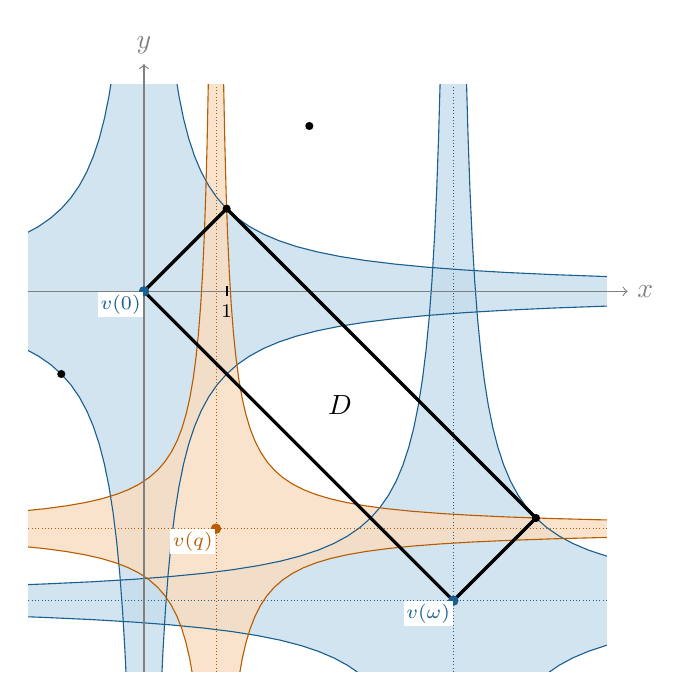
\begin{tikzpicture}[scale=1.05]
\begin{scope}\clip (-1.4,-4.6) rectangle (5.6,2.5);
\fill[regA!25, opacity=.8] (40,0.025) -- (35.3719,0.0283) -- (31.2792,0.032) -- (27.6601,0.0362) -- (24.4597,0.0409) -- (21.6297,0.0462) -- (19.127,0.0523) -- (16.914,0.0591) -- (14.957,0.0669) -- (13.2264,0.0756) -- (11.6961,0.0855) -- (10.3428,0.0967) -- (9.1461,0.1093) -- (8.0879,0.1236) -- (7.1521,0.1398) -- (6.3246,0.1581) -- (5.5928,0.1788) -- (4.9457,0.2022) -- (4.3734,0.2287) -- (3.8674,0.2586) -- (3.42,0.2924) -- (3.0243,0.3307) -- (2.6743,0.3739) -- (2.3649,0.4228) -- (2.0913,0.4782) -- (1.8493,0.5407) -- (1.6353,0.6115) -- (1.4461,0.6915) -- (1.2788,0.782) -- (1.1308,0.8843) -- (1,1) -- (0.8843,1.1308) -- (0.782,1.2788) -- (0.6915,1.4461) -- (0.6115,1.6353) -- (0.5407,1.8493) -- (0.4782,2.0913) -- (0.4228,2.3649) -- (0.3739,2.6743) -- (0.3307,3.0243) -- (0.2924,3.42) -- (0.2586,3.8674) -- (0.2287,4.3734) -- (0.2022,4.9457) -- (0.1788,5.5928) -- (0.1581,6.3246) -- (0.1398,7.1521) -- (0.1236,8.0879) -- (0.1093,9.1461) -- (0.0967,10.3428) -- (0.0855,11.6961) -- (0.0756,13.2264) -- (0.0669,14.957) -- (0.0591,16.914) -- (0.0523,19.127) -- (0.0462,21.6297) -- (0.0409,24.4597) -- (0.0362,27.6601) -- (0.032,31.2792) -- (0.0283,35.3719) -- (0.025,40) -- (-0.025,40) -- (-0.0283,35.3719) -- (-0.032,31.2792) -- (-0.0362,27.6601) -- (-0.0409,24.4597) -- (-0.0462,21.6297) -- (-0.0523,19.127) -- (-0.0591,16.914) -- (-0.0669,14.957) -- (-0.0756,13.2264) -- (-0.0855,11.6961) -- (-0.0967,10.3428) -- (-0.1093,9.1461) -- (-0.1236,8.0879) -- (-0.1398,7.1521) -- (-0.1581,6.3246) -- (-0.1788,5.5928) -- (-0.2022,4.9457) -- (-0.2287,4.3734) -- (-0.2586,3.8674) -- (-0.2924,3.42) -- (-0.3307,3.0243) -- (-0.3739,2.6743) -- (-0.4228,2.3649) -- (-0.4782,2.0913) -- (-0.5407,1.8493) -- (-0.6115,1.6353) -- (-0.6915,1.4461) -- (-0.782,1.2788) -- (-0.8843,1.1308) -- (-1,1) -- (-1.1308,0.8843) -- (-1.2788,0.782) -- (-1.4461,0.6915) -- (-1.6353,0.6115) -- (-1.8493,0.5407) -- (-2.0913,0.4782) -- (-2.3649,0.4228) -- (-2.6743,0.3739) -- (-3.0243,0.3307) -- (-3.42,0.2924) -- (-3.8674,0.2586) -- (-4.3734,0.2287) -- (-4.9457,0.2022) -- (-5.5928,0.1788) -- (-6.3246,0.1581) -- (-7.1521,0.1398) -- (-8.0879,0.1236) -- (-9.1461,0.1093) -- (-10.3428,0.0967) -- (-11.6961,0.0855) -- (-13.2264,0.0756) -- (-14.957,0.0669) -- (-16.914,0.0591) -- (-19.127,0.0523) -- (-21.6297,0.0462) -- (-24.4597,0.0409) -- (-27.6601,0.0362) -- (-31.2792,0.032) -- (-35.3719,0.0283) -- (-40,0.025) -- (-40,-0.025) -- (-35.3719,-0.0283) -- (-31.2792,-0.032) -- (-27.6601,-0.0362) -- (-24.4597,-0.0409) -- (-21.6297,-0.0462) -- (-19.127,-0.0523) -- (-16.914,-0.0591) -- (-14.957,-0.0669) -- (-13.2264,-0.0756) -- (-11.6961,-0.0855) -- (-10.3428,-0.0967) -- (-9.1461,-0.1093) -- (-8.0879,-0.1236) -- (-7.1521,-0.1398) -- (-6.3246,-0.1581) -- (-5.5928,-0.1788) -- (-4.9457,-0.2022) -- (-4.3734,-0.2287) -- (-3.8674,-0.2586) -- (-3.42,-0.2924) -- (-3.0243,-0.3307) -- (-2.6743,-0.3739) -- (-2.3649,-0.4228) -- (-2.0913,-0.4782) -- (-1.8493,-0.5407) -- (-1.6353,-0.6115) -- (-1.4461,-0.6915) -- (-1.2788,-0.782) -- (-1.1308,-0.8843) -- (-1,-1) -- (-0.8843,-1.1308) -- (-0.782,-1.2788) -- (-0.6915,-1.4461) -- (-0.6115,-1.6353) -- (-0.5407,-1.8493) -- (-0.4782,-2.0913) -- (-0.4228,-2.3649) -- (-0.3739,-2.6743) -- (-0.3307,-3.0243) -- (-0.2924,-3.42) -- (-0.2586,-3.8674) -- (-0.2287,-4.3734) -- (-0.2022,-4.9457) -- (-0.1788,-5.5928) -- (-0.1581,-6.3246) -- (-0.1398,-7.1521) -- (-0.1236,-8.0879) -- (-0.1093,-9.1461) -- (-0.0967,-10.3428) -- (-0.0855,-11.6961) -- (-0.0756,-13.2264) -- (-0.0669,-14.957) -- (-0.0591,-16.914) -- (-0.0523,-19.127) -- (-0.0462,-21.6297) -- (-0.0409,-24.4597) -- (-0.0362,-27.6601) -- (-0.032,-31.2792) -- (-0.0283,-35.3719) -- (-0.025,-40) -- (0.025,-40) -- (0.0283,-35.3719) -- (0.032,-31.2792) -- (0.0362,-27.6601) -- (0.0409,-24.4597) -- (0.0462,-21.6297) -- (0.0523,-19.127) -- (0.0591,-16.914) -- (0.0669,-14.957) -- (0.0756,-13.2264) -- (0.0855,-11.6961) -- (0.0967,-10.3428) -- (0.1093,-9.1461) -- (0.1236,-8.0879) -- (0.1398,-7.1521) -- (0.1581,-6.3246) -- (0.1788,-5.5928) -- (0.2022,-4.9457) -- (0.2287,-4.3734) -- (0.2586,-3.8674) -- (0.2924,-3.42) -- (0.3307,-3.0243) -- (0.3739,-2.6743) -- (0.4228,-2.3649) -- (0.4782,-2.0913) -- (0.5407,-1.8493) -- (0.6115,-1.6353) -- (0.6915,-1.4461) -- (0.782,-1.2788) -- (0.8843,-1.1308) -- (1,-1) -- (1.1308,-0.8843) -- (1.2788,-0.782) -- (1.4461,-0.6915) -- (1.6353,-0.6115) -- (1.8493,-0.5407) -- (2.0913,-0.4782) -- (2.3649,-0.4228) -- (2.6743,-0.3739) -- (3.0243,-0.3307) -- (3.42,-0.2924) -- (3.8674,-0.2586) -- (4.3734,-0.2287) -- (4.9457,-0.2022) -- (5.5928,-0.1788) -- (6.3246,-0.1581) -- (7.1521,-0.1398) -- (8.0879,-0.1236) -- (9.1461,-0.1093) -- (10.3428,-0.0967) -- (11.6961,-0.0855) -- (13.2264,-0.0756) -- (14.957,-0.0669) -- (16.914,-0.0591) -- (19.127,-0.0523) -- (21.6297,-0.0462) -- (24.4597,-0.0409) -- (27.6601,-0.0362) -- (31.2792,-0.032) -- (35.3719,-0.0283) -- (40,-0.025) -- cycle;
\fill[regA!25, opacity=.8] (43.7417,-3.7167) -- (39.1135,-3.7134) -- (35.0209,-3.7097) -- (31.4018,-3.7055) -- (28.2014,-3.7008) -- (25.3713,-3.6954) -- (22.8687,-3.6894) -- (20.6556,-3.6825) -- (18.6986,-3.6748) -- (16.9681,-3.6661) -- (15.4377,-3.6562) -- (14.0845,-3.645) -- (12.8878,-3.6323) -- (11.8295,-3.618) -- (10.8937,-3.6018) -- (10.0662,-3.5835) -- (9.3344,-3.5629) -- (8.6873,-3.5395) -- (8.1151,-3.513) -- (7.6091,-3.4831) -- (7.1616,-3.4493) -- (6.7659,-3.411) -- (6.416,-3.3677) -- (6.1066,-3.3188) -- (5.8329,-3.2635) -- (5.591,-3.2009) -- (5.377,-3.1302) -- (5.1878,-3.0502) -- (5.0205,-2.9597) -- (4.8725,-2.8574) -- (4.7417,-2.7417) -- (4.626,-2.6108) -- (4.5236,-2.4629) -- (4.4332,-2.2955) -- (4.3532,-2.1063) -- (4.2824,-1.8923) -- (4.2198,-1.6504) -- (4.1645,-1.3768) -- (4.1156,-1.0673) -- (4.0723,-0.7174) -- (4.0341,-0.3217) -- (4.0002,0.1258) -- (3.9703,0.6318) -- (3.9439,1.204) -- (3.9205,1.8511) -- (3.8998,2.5829) -- (3.8815,3.4104) -- (3.8653,4.3462) -- (3.851,5.4044) -- (3.8383,6.6011) -- (3.8272,7.9544) -- (3.8173,9.4848) -- (3.8085,11.2153) -- (3.8008,13.1723) -- (3.7939,15.3854) -- (3.7879,17.888) -- (3.7825,20.7181) -- (3.7778,23.9185) -- (3.7736,27.5376) -- (3.7699,31.6302) -- (3.7667,36.2583) -- (3.7167,36.2583) -- (3.7134,31.6302) -- (3.7097,27.5376) -- (3.7055,23.9185) -- (3.7008,20.7181) -- (3.6954,17.888) -- (3.6894,15.3854) -- (3.6825,13.1723) -- (3.6748,11.2153) -- (3.6661,9.4848) -- (3.6562,7.9544) -- (3.645,6.6011) -- (3.6323,5.4044) -- (3.618,4.3462) -- (3.6018,3.4104) -- (3.5835,2.5829) -- (3.5629,1.8511) -- (3.5395,1.204) -- (3.513,0.6318) -- (3.4831,0.1258) -- (3.4493,-0.3217) -- (3.411,-0.7174) -- (3.3677,-1.0673) -- (3.3188,-1.3768) -- (3.2635,-1.6504) -- (3.2009,-1.8923) -- (3.1302,-2.1063) -- (3.0502,-2.2955) -- (2.9597,-2.4629) -- (2.8574,-2.6108) -- (2.7417,-2.7417) -- (2.6108,-2.8574) -- (2.4629,-2.9597) -- (2.2955,-3.0502) -- (2.1063,-3.1302) -- (1.8923,-3.2009) -- (1.6504,-3.2635) -- (1.3768,-3.3188) -- (1.0673,-3.3677) -- (0.7174,-3.411) -- (0.3217,-3.4493) -- (-0.1258,-3.4831) -- (-0.6318,-3.513) -- (-1.204,-3.5395) -- (-1.8511,-3.5629) -- (-2.5829,-3.5835) -- (-3.4104,-3.6018) -- (-4.3462,-3.618) -- (-5.4044,-3.6323) -- (-6.6011,-3.645) -- (-7.9544,-3.6562) -- (-9.4848,-3.6661) -- (-11.2153,-3.6748) -- (-13.1723,-3.6825) -- (-15.3854,-3.6894) -- (-17.888,-3.6954) -- (-20.7181,-3.7008) -- (-23.9185,-3.7055) -- (-27.5376,-3.7097) -- (-31.6302,-3.7134) -- (-36.2583,-3.7167) -- (-36.2583,-3.7667) -- (-31.6302,-3.7699) -- (-27.5376,-3.7736) -- (-23.9185,-3.7778) -- (-20.7181,-3.7825) -- (-17.888,-3.7879) -- (-15.3854,-3.7939) -- (-13.1723,-3.8008) -- (-11.2153,-3.8085) -- (-9.4848,-3.8173) -- (-7.9544,-3.8272) -- (-6.6011,-3.8383) -- (-5.4044,-3.851) -- (-4.3462,-3.8653) -- (-3.4104,-3.8815) -- (-2.5829,-3.8998) -- (-1.8511,-3.9205) -- (-1.204,-3.9439) -- (-0.6318,-3.9703) -- (-0.1258,-4.0002) -- (0.3217,-4.0341) -- (0.7174,-4.0723) -- (1.0673,-4.1156) -- (1.3768,-4.1645) -- (1.6504,-4.2198) -- (1.8923,-4.2824) -- (2.1063,-4.3532) -- (2.2955,-4.4332) -- (2.4629,-4.5236) -- (2.6108,-4.626) -- (2.7417,-4.7417) -- (2.8574,-4.8725) -- (2.9597,-5.0205) -- (3.0502,-5.1878) -- (3.1302,-5.377) -- (3.2009,-5.591) -- (3.2635,-5.8329) -- (3.3188,-6.1066) -- (3.3677,-6.416) -- (3.411,-6.7659) -- (3.4493,-7.1616) -- (3.4831,-7.6091) -- (3.513,-8.1151) -- (3.5395,-8.6873) -- (3.5629,-9.3344) -- (3.5835,-10.0662) -- (3.6018,-10.8937) -- (3.618,-11.8295) -- (3.6323,-12.8878) -- (3.645,-14.0845) -- (3.6562,-15.4377) -- (3.6661,-16.9681) -- (3.6748,-18.6986) -- (3.6825,-20.6556) -- (3.6894,-22.8687) -- (3.6954,-25.3713) -- (3.7008,-28.2014) -- (3.7055,-31.4018) -- (3.7097,-35.0209) -- (3.7134,-39.1135) -- (3.7167,-43.7417) -- (3.7667,-43.7417) -- (3.7699,-39.1135) -- (3.7736,-35.0209) -- (3.7778,-31.4018) -- (3.7825,-28.2014) -- (3.7879,-25.3713) -- (3.7939,-22.8687) -- (3.8008,-20.6556) -- (3.8085,-18.6986) -- (3.8173,-16.9681) -- (3.8272,-15.4377) -- (3.8383,-14.0845) -- (3.851,-12.8878) -- (3.8653,-11.8295) -- (3.8815,-10.8937) -- (3.8998,-10.0662) -- (3.9205,-9.3344) -- (3.9439,-8.6873) -- (3.9703,-8.1151) -- (4.0002,-7.6091) -- (4.0341,-7.1616) -- (4.0723,-6.7659) -- (4.1156,-6.416) -- (4.1645,-6.1066) -- (4.2198,-5.8329) -- (4.2824,-5.591) -- (4.3532,-5.377) -- (4.4332,-5.1878) -- (4.5236,-5.0205) -- (4.626,-4.8725) -- (4.7417,-4.7417) -- (4.8725,-4.626) -- (5.0205,-4.5236) -- (5.1878,-4.4332) -- (5.377,-4.3532) -- (5.591,-4.2824) -- (5.8329,-4.2198) -- (6.1066,-4.1645) -- (6.416,-4.1156) -- (6.7659,-4.0723) -- (7.1616,-4.0341) -- (7.6091,-4.0002) -- (8.1151,-3.9703) -- (8.6873,-3.9439) -- (9.3344,-3.9205) -- (10.0662,-3.8998) -- (10.8937,-3.8815) -- (11.8295,-3.8653) -- (12.8878,-3.851) -- (14.0845,-3.8383) -- (15.4377,-3.8272) -- (16.9681,-3.8173) -- (18.6986,-3.8085) -- (20.6556,-3.8008) -- (22.8687,-3.7939) -- (25.3713,-3.7879) -- (28.2014,-3.7825) -- (31.4018,-3.7778) -- (35.0209,-3.7736) -- (39.1135,-3.7699) -- (43.7417,-3.7667) -- cycle;
\fill[regB!25, opacity=.8] (40.8708,-2.8583) -- (35.8364,-2.8565) -- (31.4356,-2.8545) -- (27.5887,-2.8521) -- (24.226,-2.8494) -- (21.2865,-2.8463) -- (18.717,-2.8428) -- (16.4709,-2.8388) -- (14.5074,-2.8342) -- (12.7911,-2.8289) -- (11.2908,-2.8228) -- (9.9794,-2.8159) -- (8.833,-2.808) -- (7.8309,-2.799) -- (6.9549,-2.7886) -- (6.1891,-2.7768) -- (5.5198,-2.7633) -- (4.9346,-2.7478) -- (4.4232,-2.7301) -- (3.9761,-2.7098) -- (3.5852,-2.6866) -- (3.2436,-2.6601) -- (2.945,-2.6298) -- (2.6839,-2.5951) -- (2.4557,-2.5554) -- (2.2562,-2.5099) -- (2.0819,-2.458) -- (1.9295,-2.3985) -- (1.7962,-2.3305) -- (1.6797,-2.2527) -- (1.5779,-2.1637) -- (1.4889,-2.0619) -- (1.4111,-1.9454) -- (1.3431,-1.8122) -- (1.2837,-1.6598) -- (1.2317,-1.4854) -- (1.1863,-1.2859) -- (1.1466,-1.0577) -- (1.1119,-0.7967) -- (1.0816,-0.498) -- (1.055,-0.1564) -- (1.0318,0.2344) -- (1.0116,0.6815) -- (0.9939,1.193) -- (0.9784,1.7781) -- (0.9648,2.4475) -- (0.953,3.2132) -- (0.9427,4.0892) -- (0.9336,5.0913) -- (0.9257,6.2377) -- (0.9188,7.5492) -- (0.9128,9.0495) -- (0.9075,10.7658) -- (0.9029,12.7292) -- (0.8988,14.9753) -- (0.8953,17.5449) -- (0.8922,20.4844) -- (0.8895,23.8471) -- (0.8872,27.694) -- (0.8851,32.0948) -- (0.8833,37.1292) -- (0.8583,37.1292) -- (0.8565,32.0948) -- (0.8545,27.694) -- (0.8521,23.8471) -- (0.8494,20.4844) -- (0.8463,17.5449) -- (0.8428,14.9753) -- (0.8388,12.7292) -- (0.8342,10.7658) -- (0.8289,9.0495) -- (0.8228,7.5492) -- (0.8159,6.2377) -- (0.808,5.0913) -- (0.799,4.0892) -- (0.7886,3.2132) -- (0.7768,2.4475) -- (0.7633,1.7781) -- (0.7478,1.193) -- (0.7301,0.6815) -- (0.7098,0.2344) -- (0.6866,-0.1564) -- (0.6601,-0.498) -- (0.6298,-0.7967) -- (0.5951,-1.0577) -- (0.5554,-1.2859) -- (0.5099,-1.4854) -- (0.458,-1.6598) -- (0.3985,-1.8122) -- (0.3305,-1.9454) -- (0.2527,-2.0619) -- (0.1637,-2.1637) -- (0.0619,-2.2527) -- (-0.0546,-2.3305) -- (-0.1878,-2.3985) -- (-0.3402,-2.458) -- (-0.5146,-2.5099) -- (-0.7141,-2.5554) -- (-0.9423,-2.5951) -- (-1.2033,-2.6298) -- (-1.502,-2.6601) -- (-1.8436,-2.6866) -- (-2.2344,-2.7098) -- (-2.6815,-2.7301) -- (-3.193,-2.7478) -- (-3.7781,-2.7633) -- (-4.4475,-2.7768) -- (-5.2132,-2.7886) -- (-6.0892,-2.799) -- (-7.0913,-2.808) -- (-8.2377,-2.8159) -- (-9.5492,-2.8228) -- (-11.0495,-2.8289) -- (-12.7658,-2.8342) -- (-14.7292,-2.8388) -- (-16.9753,-2.8428) -- (-19.5449,-2.8463) -- (-22.4844,-2.8494) -- (-25.8471,-2.8521) -- (-29.694,-2.8545) -- (-34.0948,-2.8565) -- (-39.1292,-2.8583) -- (-39.1292,-2.8833) -- (-34.0948,-2.8851) -- (-29.694,-2.8872) -- (-25.8471,-2.8895) -- (-22.4844,-2.8922) -- (-19.5449,-2.8953) -- (-16.9753,-2.8988) -- (-14.7292,-2.9029) -- (-12.7658,-2.9075) -- (-11.0495,-2.9128) -- (-9.5492,-2.9188) -- (-8.2377,-2.9257) -- (-7.0913,-2.9336) -- (-6.0892,-2.9427) -- (-5.2132,-2.953) -- (-4.4475,-2.9648) -- (-3.7781,-2.9784) -- (-3.193,-2.9939) -- (-2.6815,-3.0116) -- (-2.2344,-3.0318) -- (-1.8436,-3.055) -- (-1.502,-3.0816) -- (-1.2033,-3.1119) -- (-0.9423,-3.1466) -- (-0.7141,-3.1863) -- (-0.5146,-3.2317) -- (-0.3402,-3.2837) -- (-0.1878,-3.3431) -- (-0.0546,-3.4111) -- (0.0619,-3.4889) -- (0.1637,-3.5779) -- (0.2527,-3.6797) -- (0.3305,-3.7962) -- (0.3985,-3.9295) -- (0.458,-4.0819) -- (0.5099,-4.2562) -- (0.5554,-4.4557) -- (0.5951,-4.6839) -- (0.6298,-4.945) -- (0.6601,-5.2436) -- (0.6866,-5.5852) -- (0.7098,-5.9761) -- (0.7301,-6.4232) -- (0.7478,-6.9346) -- (0.7633,-7.5198) -- (0.7768,-8.1891) -- (0.7886,-8.9549) -- (0.799,-9.8309) -- (0.808,-10.833) -- (0.8159,-11.9794) -- (0.8228,-13.2908) -- (0.8289,-14.7911) -- (0.8342,-16.5074) -- (0.8388,-18.4709) -- (0.8428,-20.717) -- (0.8463,-23.2865) -- (0.8494,-26.226) -- (0.8521,-29.5887) -- (0.8545,-33.4356) -- (0.8565,-37.8364) -- (0.8583,-42.8708) -- (0.8833,-42.8708) -- (0.8851,-37.8364) -- (0.8872,-33.4356) -- (0.8895,-29.5887) -- (0.8922,-26.226) -- (0.8953,-23.2865) -- (0.8988,-20.717) -- (0.9029,-18.4709) -- (0.9075,-16.5074) -- (0.9128,-14.7911) -- (0.9188,-13.2908) -- (0.9257,-11.9794) -- (0.9336,-10.833) -- (0.9427,-9.8309) -- (0.953,-8.9549) -- (0.9648,-8.1891) -- (0.9784,-7.5198) -- (0.9939,-6.9346) -- (1.0116,-6.4232) -- (1.0318,-5.9761) -- (1.055,-5.5852) -- (1.0816,-5.2436) -- (1.1119,-4.945) -- (1.1466,-4.6839) -- (1.1863,-4.4557) -- (1.2317,-4.2562) -- (1.2837,-4.0819) -- (1.3431,-3.9295) -- (1.4111,-3.7962) -- (1.4889,-3.6797) -- (1.5779,-3.5779) -- (1.6797,-3.4889) -- (1.7962,-3.4111) -- (1.9295,-3.3431) -- (2.0819,-3.2837) -- (2.2562,-3.2317) -- (2.4557,-3.1863) -- (2.6839,-3.1466) -- (2.945,-3.1119) -- (3.2436,-3.0816) -- (3.5852,-3.055) -- (3.9761,-3.0318) -- (4.4232,-3.0116) -- (4.9346,-2.9939) -- (5.5198,-2.9784) -- (6.1891,-2.9648) -- (6.9549,-2.953) -- (7.8309,-2.9427) -- (8.833,-2.9336) -- (9.9794,-2.9257) -- (11.2908,-2.9188) -- (12.7911,-2.9128) -- (14.5074,-2.9075) -- (16.4709,-2.9029) -- (18.717,-2.8988) -- (21.2865,-2.8953) -- (24.226,-2.8922) -- (27.5887,-2.8895) -- (31.4356,-2.8872) -- (35.8364,-2.8851) -- (40.8708,-2.8833) -- cycle;
\draw[regA!80!black, thin] (0.025,40) -- (0.0283,35.3719) -- (0.032,31.2792) -- (0.0362,27.6601) -- (0.0409,24.4597) -- (0.0462,21.6297) -- (0.0523,19.127) -- (0.0591,16.914) -- (0.0669,14.957) -- (0.0756,13.2264) -- (0.0855,11.6961) -- (0.0967,10.3428) -- (0.1093,9.1461) -- (0.1236,8.0879) -- (0.1398,7.1521) -- (0.1581,6.3246) -- (0.1788,5.5928) -- (0.2022,4.9457) -- (0.2287,4.3734) -- (0.2586,3.8674) -- (0.2924,3.42) -- (0.3307,3.0243) -- (0.3739,2.6743) -- (0.4228,2.3649) -- (0.4782,2.0913) -- (0.5407,1.8493) -- (0.6115,1.6353) -- (0.6915,1.4461) -- (0.782,1.2788) -- (0.8843,1.1308) -- (1,1) -- (1.1308,0.8843) -- (1.2788,0.782) -- (1.4461,0.6915) -- (1.6353,0.6115) -- (1.8493,0.5407) -- (2.0913,0.4782) -- (2.3649,0.4228) -- (2.6743,0.3739) -- (3.0243,0.3307) -- (3.42,0.2924) -- (3.8674,0.2586) -- (4.3734,0.2287) -- (4.9457,0.2022) -- (5.5928,0.1788) -- (6.3246,0.1581) -- (7.1521,0.1398) -- (8.0879,0.1236) -- (9.1461,0.1093) -- (10.3428,0.0967) -- (11.6961,0.0855) -- (13.2264,0.0756) -- (14.957,0.0669) -- (16.914,0.0591) -- (19.127,0.0523) -- (21.6297,0.0462) -- (24.4597,0.0409) -- (27.6601,0.0362) -- (31.2792,0.032) -- (35.3719,0.0283) -- (40,0.025);
\draw[regA!80!black, thin] (-0.025,40) -- (-0.0283,35.3719) -- (-0.032,31.2792) -- (-0.0362,27.6601) -- (-0.0409,24.4597) -- (-0.0462,21.6297) -- (-0.0523,19.127) -- (-0.0591,16.914) -- (-0.0669,14.957) -- (-0.0756,13.2264) -- (-0.0855,11.6961) -- (-0.0967,10.3428) -- (-0.1093,9.1461) -- (-0.1236,8.0879) -- (-0.1398,7.1521) -- (-0.1581,6.3246) -- (-0.1788,5.5928) -- (-0.2022,4.9457) -- (-0.2287,4.3734) -- (-0.2586,3.8674) -- (-0.2924,3.42) -- (-0.3307,3.0243) -- (-0.3739,2.6743) -- (-0.4228,2.3649) -- (-0.4782,2.0913) -- (-0.5407,1.8493) -- (-0.6115,1.6353) -- (-0.6915,1.4461) -- (-0.782,1.2788) -- (-0.8843,1.1308) -- (-1,1) -- (-1.1308,0.8843) -- (-1.2788,0.782) -- (-1.4461,0.6915) -- (-1.6353,0.6115) -- (-1.8493,0.5407) -- (-2.0913,0.4782) -- (-2.3649,0.4228) -- (-2.6743,0.3739) -- (-3.0243,0.3307) -- (-3.42,0.2924) -- (-3.8674,0.2586) -- (-4.3734,0.2287) -- (-4.9457,0.2022) -- (-5.5928,0.1788) -- (-6.3246,0.1581) -- (-7.1521,0.1398) -- (-8.0879,0.1236) -- (-9.1461,0.1093) -- (-10.3428,0.0967) -- (-11.6961,0.0855) -- (-13.2264,0.0756) -- (-14.957,0.0669) -- (-16.914,0.0591) -- (-19.127,0.0523) -- (-21.6297,0.0462) -- (-24.4597,0.0409) -- (-27.6601,0.0362) -- (-31.2792,0.032) -- (-35.3719,0.0283) -- (-40,0.025);
\draw[regA!80!black, thin] (-0.025,-40) -- (-0.0283,-35.3719) -- (-0.032,-31.2792) -- (-0.0362,-27.6601) -- (-0.0409,-24.4597) -- (-0.0462,-21.6297) -- (-0.0523,-19.127) -- (-0.0591,-16.914) -- (-0.0669,-14.957) -- (-0.0756,-13.2264) -- (-0.0855,-11.6961) -- (-0.0967,-10.3428) -- (-0.1093,-9.1461) -- (-0.1236,-8.0879) -- (-0.1398,-7.1521) -- (-0.1581,-6.3246) -- (-0.1788,-5.5928) -- (-0.2022,-4.9457) -- (-0.2287,-4.3734) -- (-0.2586,-3.8674) -- (-0.2924,-3.42) -- (-0.3307,-3.0243) -- (-0.3739,-2.6743) -- (-0.4228,-2.3649) -- (-0.4782,-2.0913) -- (-0.5407,-1.8493) -- (-0.6115,-1.6353) -- (-0.6915,-1.4461) -- (-0.782,-1.2788) -- (-0.8843,-1.1308) -- (-1,-1) -- (-1.1308,-0.8843) -- (-1.2788,-0.782) -- (-1.4461,-0.6915) -- (-1.6353,-0.6115) -- (-1.8493,-0.5407) -- (-2.0913,-0.4782) -- (-2.3649,-0.4228) -- (-2.6743,-0.3739) -- (-3.0243,-0.3307) -- (-3.42,-0.2924) -- (-3.8674,-0.2586) -- (-4.3734,-0.2287) -- (-4.9457,-0.2022) -- (-5.5928,-0.1788) -- (-6.3246,-0.1581) -- (-7.1521,-0.1398) -- (-8.0879,-0.1236) -- (-9.1461,-0.1093) -- (-10.3428,-0.0967) -- (-11.6961,-0.0855) -- (-13.2264,-0.0756) -- (-14.957,-0.0669) -- (-16.914,-0.0591) -- (-19.127,-0.0523) -- (-21.6297,-0.0462) -- (-24.4597,-0.0409) -- (-27.6601,-0.0362) -- (-31.2792,-0.032) -- (-35.3719,-0.0283) -- (-40,-0.025);
\draw[regA!80!black, thin] (0.025,-40) -- (0.0283,-35.3719) -- (0.032,-31.2792) -- (0.0362,-27.6601) -- (0.0409,-24.4597) -- (0.0462,-21.6297) -- (0.0523,-19.127) -- (0.0591,-16.914) -- (0.0669,-14.957) -- (0.0756,-13.2264) -- (0.0855,-11.6961) -- (0.0967,-10.3428) -- (0.1093,-9.1461) -- (0.1236,-8.0879) -- (0.1398,-7.1521) -- (0.1581,-6.3246) -- (0.1788,-5.5928) -- (0.2022,-4.9457) -- (0.2287,-4.3734) -- (0.2586,-3.8674) -- (0.2924,-3.42) -- (0.3307,-3.0243) -- (0.3739,-2.6743) -- (0.4228,-2.3649) -- (0.4782,-2.0913) -- (0.5407,-1.8493) -- (0.6115,-1.6353) -- (0.6915,-1.4461) -- (0.782,-1.2788) -- (0.8843,-1.1308) -- (1,-1) -- (1.1308,-0.8843) -- (1.2788,-0.782) -- (1.4461,-0.6915) -- (1.6353,-0.6115) -- (1.8493,-0.5407) -- (2.0913,-0.4782) -- (2.3649,-0.4228) -- (2.6743,-0.3739) -- (3.0243,-0.3307) -- (3.42,-0.2924) -- (3.8674,-0.2586) -- (4.3734,-0.2287) -- (4.9457,-0.2022) -- (5.5928,-0.1788) -- (6.3246,-0.1581) -- (7.1521,-0.1398) -- (8.0879,-0.1236) -- (9.1461,-0.1093) -- (10.3428,-0.0967) -- (11.6961,-0.0855) -- (13.2264,-0.0756) -- (14.957,-0.0669) -- (16.914,-0.0591) -- (19.127,-0.0523) -- (21.6297,-0.0462) -- (24.4597,-0.0409) -- (27.6601,-0.0362) -- (31.2792,-0.032) -- (35.3719,-0.0283) -- (40,-0.025);
\draw[regA!80!black, densely dotted, very thin] (0,-4.6) -- (0,2.5) (-1.4,0) -- (5.6,0);
\draw[regA!80!black, thin] (3.7667,36.2583) -- (3.7699,31.6302) -- (3.7736,27.5376) -- (3.7778,23.9185) -- (3.7825,20.7181) -- (3.7879,17.888) -- (3.7939,15.3854) -- (3.8008,13.1723) -- (3.8085,11.2153) -- (3.8173,9.4848) -- (3.8272,7.9544) -- (3.8383,6.6011) -- (3.851,5.4044) -- (3.8653,4.3462) -- (3.8815,3.4104) -- (3.8998,2.5829) -- (3.9205,1.8511) -- (3.9439,1.204) -- (3.9703,0.6318) -- (4.0002,0.1258) -- (4.0341,-0.3217) -- (4.0723,-0.7174) -- (4.1156,-1.0673) -- (4.1645,-1.3768) -- (4.2198,-1.6504) -- (4.2824,-1.8923) -- (4.3532,-2.1063) -- (4.4332,-2.2955) -- (4.5236,-2.4629) -- (4.626,-2.6108) -- (4.7417,-2.7417) -- (4.8725,-2.8574) -- (5.0205,-2.9597) -- (5.1878,-3.0502) -- (5.377,-3.1302) -- (5.591,-3.2009) -- (5.8329,-3.2635) -- (6.1066,-3.3188) -- (6.416,-3.3677) -- (6.7659,-3.411) -- (7.1616,-3.4493) -- (7.6091,-3.4831) -- (8.1151,-3.513) -- (8.6873,-3.5395) -- (9.3344,-3.5629) -- (10.0662,-3.5835) -- (10.8937,-3.6018) -- (11.8295,-3.618) -- (12.8878,-3.6323) -- (14.0845,-3.645) -- (15.4377,-3.6562) -- (16.9681,-3.6661) -- (18.6986,-3.6748) -- (20.6556,-3.6825) -- (22.8687,-3.6894) -- (25.3713,-3.6954) -- (28.2014,-3.7008) -- (31.4018,-3.7055) -- (35.0209,-3.7097) -- (39.1135,-3.7134) -- (43.7417,-3.7167);
\draw[regA!80!black, thin] (3.7167,36.2583) -- (3.7134,31.6302) -- (3.7097,27.5376) -- (3.7055,23.9185) -- (3.7008,20.7181) -- (3.6954,17.888) -- (3.6894,15.3854) -- (3.6825,13.1723) -- (3.6748,11.2153) -- (3.6661,9.4848) -- (3.6562,7.9544) -- (3.645,6.6011) -- (3.6323,5.4044) -- (3.618,4.3462) -- (3.6018,3.4104) -- (3.5835,2.5829) -- (3.5629,1.8511) -- (3.5395,1.204) -- (3.513,0.6318) -- (3.4831,0.1258) -- (3.4493,-0.3217) -- (3.411,-0.7174) -- (3.3677,-1.0673) -- (3.3188,-1.3768) -- (3.2635,-1.6504) -- (3.2009,-1.8923) -- (3.1302,-2.1063) -- (3.0502,-2.2955) -- (2.9597,-2.4629) -- (2.8574,-2.6108) -- (2.7417,-2.7417) -- (2.6108,-2.8574) -- (2.4629,-2.9597) -- (2.2955,-3.0502) -- (2.1063,-3.1302) -- (1.8923,-3.2009) -- (1.6504,-3.2635) -- (1.3768,-3.3188) -- (1.0673,-3.3677) -- (0.7174,-3.411) -- (0.3217,-3.4493) -- (-0.1258,-3.4831) -- (-0.6318,-3.513) -- (-1.204,-3.5395) -- (-1.8511,-3.5629) -- (-2.5829,-3.5835) -- (-3.4104,-3.6018) -- (-4.3462,-3.618) -- (-5.4044,-3.6323) -- (-6.6011,-3.645) -- (-7.9544,-3.6562) -- (-9.4848,-3.6661) -- (-11.2153,-3.6748) -- (-13.1723,-3.6825) -- (-15.3854,-3.6894) -- (-17.888,-3.6954) -- (-20.7181,-3.7008) -- (-23.9185,-3.7055) -- (-27.5376,-3.7097) -- (-31.6302,-3.7134) -- (-36.2583,-3.7167);
\draw[regA!80!black, thin] (3.7167,-43.7417) -- (3.7134,-39.1135) -- (3.7097,-35.0209) -- (3.7055,-31.4018) -- (3.7008,-28.2014) -- (3.6954,-25.3713) -- (3.6894,-22.8687) -- (3.6825,-20.6556) -- (3.6748,-18.6986) -- (3.6661,-16.9681) -- (3.6562,-15.4377) -- (3.645,-14.0845) -- (3.6323,-12.8878) -- (3.618,-11.8295) -- (3.6018,-10.8937) -- (3.5835,-10.0662) -- (3.5629,-9.3344) -- (3.5395,-8.6873) -- (3.513,-8.1151) -- (3.4831,-7.6091) -- (3.4493,-7.1616) -- (3.411,-6.7659) -- (3.3677,-6.416) -- (3.3188,-6.1066) -- (3.2635,-5.8329) -- (3.2009,-5.591) -- (3.1302,-5.377) -- (3.0502,-5.1878) -- (2.9597,-5.0205) -- (2.8574,-4.8725) -- (2.7417,-4.7417) -- (2.6108,-4.626) -- (2.4629,-4.5236) -- (2.2955,-4.4332) -- (2.1063,-4.3532) -- (1.8923,-4.2824) -- (1.6504,-4.2198) -- (1.3768,-4.1645) -- (1.0673,-4.1156) -- (0.7174,-4.0723) -- (0.3217,-4.0341) -- (-0.1258,-4.0002) -- (-0.6318,-3.9703) -- (-1.204,-3.9439) -- (-1.8511,-3.9205) -- (-2.5829,-3.8998) -- (-3.4104,-3.8815) -- (-4.3462,-3.8653) -- (-5.4044,-3.851) -- (-6.6011,-3.8383) -- (-7.9544,-3.8272) -- (-9.4848,-3.8173) -- (-11.2153,-3.8085) -- (-13.1723,-3.8008) -- (-15.3854,-3.7939) -- (-17.888,-3.7879) -- (-20.7181,-3.7825) -- (-23.9185,-3.7778) -- (-27.5376,-3.7736) -- (-31.6302,-3.7699) -- (-36.2583,-3.7667);
\draw[regA!80!black, thin] (3.7667,-43.7417) -- (3.7699,-39.1135) -- (3.7736,-35.0209) -- (3.7778,-31.4018) -- (3.7825,-28.2014) -- (3.7879,-25.3713) -- (3.7939,-22.8687) -- (3.8008,-20.6556) -- (3.8085,-18.6986) -- (3.8173,-16.9681) -- (3.8272,-15.4377) -- (3.8383,-14.0845) -- (3.851,-12.8878) -- (3.8653,-11.8295) -- (3.8815,-10.8937) -- (3.8998,-10.0662) -- (3.9205,-9.3344) -- (3.9439,-8.6873) -- (3.9703,-8.1151) -- (4.0002,-7.6091) -- (4.0341,-7.1616) -- (4.0723,-6.7659) -- (4.1156,-6.416) -- (4.1645,-6.1066) -- (4.2198,-5.8329) -- (4.2824,-5.591) -- (4.3532,-5.377) -- (4.4332,-5.1878) -- (4.5236,-5.0205) -- (4.626,-4.8725) -- (4.7417,-4.7417) -- (4.8725,-4.626) -- (5.0205,-4.5236) -- (5.1878,-4.4332) -- (5.377,-4.3532) -- (5.591,-4.2824) -- (5.8329,-4.2198) -- (6.1066,-4.1645) -- (6.416,-4.1156) -- (6.7659,-4.0723) -- (7.1616,-4.0341) -- (7.6091,-4.0002) -- (8.1151,-3.9703) -- (8.6873,-3.9439) -- (9.3344,-3.9205) -- (10.0662,-3.8998) -- (10.8937,-3.8815) -- (11.8295,-3.8653) -- (12.8878,-3.851) -- (14.0845,-3.8383) -- (15.4377,-3.8272) -- (16.9681,-3.8173) -- (18.6986,-3.8085) -- (20.6556,-3.8008) -- (22.8687,-3.7939) -- (25.3713,-3.7879) -- (28.2014,-3.7825) -- (31.4018,-3.7778) -- (35.0209,-3.7736) -- (39.1135,-3.7699) -- (43.7417,-3.7667);
\draw[regA!80!black, densely dotted, very thin] (3.7417,-4.6) -- (3.7417,2.5) (-1.4,-3.7417) -- (5.6,-3.7417);
\draw[regB!80!black, thin] (0.8833,37.1292) -- (0.8851,32.0948) -- (0.8872,27.694) -- (0.8895,23.8471) -- (0.8922,20.4844) -- (0.8953,17.5449) -- (0.8988,14.9753) -- (0.9029,12.7292) -- (0.9075,10.7658) -- (0.9128,9.0495) -- (0.9188,7.5492) -- (0.9257,6.2377) -- (0.9336,5.0913) -- (0.9427,4.0892) -- (0.953,3.2132) -- (0.9648,2.4475) -- (0.9784,1.7781) -- (0.9939,1.193) -- (1.0116,0.6815) -- (1.0318,0.2344) -- (1.055,-0.1564) -- (1.0816,-0.498) -- (1.1119,-0.7967) -- (1.1466,-1.0577) -- (1.1863,-1.2859) -- (1.2317,-1.4854) -- (1.2837,-1.6598) -- (1.3431,-1.8122) -- (1.4111,-1.9454) -- (1.4889,-2.0619) -- (1.5779,-2.1637) -- (1.6797,-2.2527) -- (1.7962,-2.3305) -- (1.9295,-2.3985) -- (2.0819,-2.458) -- (2.2562,-2.5099) -- (2.4557,-2.5554) -- (2.6839,-2.5951) -- (2.945,-2.6298) -- (3.2436,-2.6601) -- (3.5852,-2.6866) -- (3.9761,-2.7098) -- (4.4232,-2.7301) -- (4.9346,-2.7478) -- (5.5198,-2.7633) -- (6.1891,-2.7768) -- (6.9549,-2.7886) -- (7.8309,-2.799) -- (8.833,-2.808) -- (9.9794,-2.8159) -- (11.2908,-2.8228) -- (12.7911,-2.8289) -- (14.5074,-2.8342) -- (16.4709,-2.8388) -- (18.717,-2.8428) -- (21.2865,-2.8463) -- (24.226,-2.8494) -- (27.5887,-2.8521) -- (31.4356,-2.8545) -- (35.8364,-2.8565) -- (40.8708,-2.8583);
\draw[regB!80!black, thin] (0.8583,37.1292) -- (0.8565,32.0948) -- (0.8545,27.694) -- (0.8521,23.8471) -- (0.8494,20.4844) -- (0.8463,17.5449) -- (0.8428,14.9753) -- (0.8388,12.7292) -- (0.8342,10.7658) -- (0.8289,9.0495) -- (0.8228,7.5492) -- (0.8159,6.2377) -- (0.808,5.0913) -- (0.799,4.0892) -- (0.7886,3.2132) -- (0.7768,2.4475) -- (0.7633,1.7781) -- (0.7478,1.193) -- (0.7301,0.6815) -- (0.7098,0.2344) -- (0.6866,-0.1564) -- (0.6601,-0.498) -- (0.6298,-0.7967) -- (0.5951,-1.0577) -- (0.5554,-1.2859) -- (0.5099,-1.4854) -- (0.458,-1.6598) -- (0.3985,-1.8122) -- (0.3305,-1.9454) -- (0.2527,-2.0619) -- (0.1637,-2.1637) -- (0.0619,-2.2527) -- (-0.0546,-2.3305) -- (-0.1878,-2.3985) -- (-0.3402,-2.458) -- (-0.5146,-2.5099) -- (-0.7141,-2.5554) -- (-0.9423,-2.5951) -- (-1.2033,-2.6298) -- (-1.502,-2.6601) -- (-1.8436,-2.6866) -- (-2.2344,-2.7098) -- (-2.6815,-2.7301) -- (-3.193,-2.7478) -- (-3.7781,-2.7633) -- (-4.4475,-2.7768) -- (-5.2132,-2.7886) -- (-6.0892,-2.799) -- (-7.0913,-2.808) -- (-8.2377,-2.8159) -- (-9.5492,-2.8228) -- (-11.0495,-2.8289) -- (-12.7658,-2.8342) -- (-14.7292,-2.8388) -- (-16.9753,-2.8428) -- (-19.5449,-2.8463) -- (-22.4844,-2.8494) -- (-25.8471,-2.8521) -- (-29.694,-2.8545) -- (-34.0948,-2.8565) -- (-39.1292,-2.8583);
\draw[regB!80!black, thin] (0.8583,-42.8708) -- (0.8565,-37.8364) -- (0.8545,-33.4356) -- (0.8521,-29.5887) -- (0.8494,-26.226) -- (0.8463,-23.2865) -- (0.8428,-20.717) -- (0.8388,-18.4709) -- (0.8342,-16.5074) -- (0.8289,-14.7911) -- (0.8228,-13.2908) -- (0.8159,-11.9794) -- (0.808,-10.833) -- (0.799,-9.8309) -- (0.7886,-8.9549) -- (0.7768,-8.1891) -- (0.7633,-7.5198) -- (0.7478,-6.9346) -- (0.7301,-6.4232) -- (0.7098,-5.9761) -- (0.6866,-5.5852) -- (0.6601,-5.2436) -- (0.6298,-4.945) -- (0.5951,-4.6839) -- (0.5554,-4.4557) -- (0.5099,-4.2562) -- (0.458,-4.0819) -- (0.3985,-3.9295) -- (0.3305,-3.7962) -- (0.2527,-3.6797) -- (0.1637,-3.5779) -- (0.0619,-3.4889) -- (-0.0546,-3.4111) -- (-0.1878,-3.3431) -- (-0.3402,-3.2837) -- (-0.5146,-3.2317) -- (-0.7141,-3.1863) -- (-0.9423,-3.1466) -- (-1.2033,-3.1119) -- (-1.502,-3.0816) -- (-1.8436,-3.055) -- (-2.2344,-3.0318) -- (-2.6815,-3.0116) -- (-3.193,-2.9939) -- (-3.7781,-2.9784) -- (-4.4475,-2.9648) -- (-5.2132,-2.953) -- (-6.0892,-2.9427) -- (-7.0913,-2.9336) -- (-8.2377,-2.9257) -- (-9.5492,-2.9188) -- (-11.0495,-2.9128) -- (-12.7658,-2.9075) -- (-14.7292,-2.9029) -- (-16.9753,-2.8988) -- (-19.5449,-2.8953) -- (-22.4844,-2.8922) -- (-25.8471,-2.8895) -- (-29.694,-2.8872) -- (-34.0948,-2.8851) -- (-39.1292,-2.8833);
\draw[regB!80!black, thin] (0.8833,-42.8708) -- (0.8851,-37.8364) -- (0.8872,-33.4356) -- (0.8895,-29.5887) -- (0.8922,-26.226) -- (0.8953,-23.2865) -- (0.8988,-20.717) -- (0.9029,-18.4709) -- (0.9075,-16.5074) -- (0.9128,-14.7911) -- (0.9188,-13.2908) -- (0.9257,-11.9794) -- (0.9336,-10.833) -- (0.9427,-9.8309) -- (0.953,-8.9549) -- (0.9648,-8.1891) -- (0.9784,-7.5198) -- (0.9939,-6.9346) -- (1.0116,-6.4232) -- (1.0318,-5.9761) -- (1.055,-5.5852) -- (1.0816,-5.2436) -- (1.1119,-4.945) -- (1.1466,-4.6839) -- (1.1863,-4.4557) -- (1.2317,-4.2562) -- (1.2837,-4.0819) -- (1.3431,-3.9295) -- (1.4111,-3.7962) -- (1.4889,-3.6797) -- (1.5779,-3.5779) -- (1.6797,-3.4889) -- (1.7962,-3.4111) -- (1.9295,-3.3431) -- (2.0819,-3.2837) -- (2.2562,-3.2317) -- (2.4557,-3.1863) -- (2.6839,-3.1466) -- (2.945,-3.1119) -- (3.2436,-3.0816) -- (3.5852,-3.055) -- (3.9761,-3.0318) -- (4.4232,-3.0116) -- (4.9346,-2.9939) -- (5.5198,-2.9784) -- (6.1891,-2.9648) -- (6.9549,-2.953) -- (7.8309,-2.9427) -- (8.833,-2.9336) -- (9.9794,-2.9257) -- (11.2908,-2.9188) -- (12.7911,-2.9128) -- (14.5074,-2.9075) -- (16.4709,-2.9029) -- (18.717,-2.8988) -- (21.2865,-2.8953) -- (24.226,-2.8922) -- (27.5887,-2.8895) -- (31.4356,-2.8872) -- (35.8364,-2.8851) -- (40.8708,-2.8833);
\draw[regB!80!black, densely dotted, very thin] (0.8708,-4.6) -- (0.8708,2.5) (-1.4,-2.8708) -- (5.6,-2.8708);
\end{scope}
\draw[->, gray] (-1.4,0) -- (5.85,0) node[right] {$x$};
\draw[->, gray] (0,-4.6) -- (0,2.75) node[above] {$y$};
\fill[black] (-1,-1) circle (1.4pt);
\fill[black] (0,0) circle (1.4pt);
\fill[black] (1,1) circle (1.4pt);
\fill[black] (2,2) circle (1.4pt);
\fill[black] (3.7417,-3.7417) circle (1.4pt);
\fill[black] (4.7417,-2.7417) circle (1.4pt);
\draw[very thick] (0,0) -- (1,1) -- (4.7417,-2.7417) -- (3.7417,-3.7417) -- cycle;
\node at (2.37,-1.37) {$D$};
\fill[regA!80!black] (0,0) circle (1.8pt) node[below left, font=\scriptsize, fill=white, inner sep=1pt] {$v(0)$};
\fill[regA!80!black] (3.7417,-3.7417) circle (1.8pt) node[below left, font=\scriptsize, fill=white, inner sep=1pt] {$v(\omega)$};
\fill[regB!80!black] (0.8708,-2.8708) circle (1.8pt) node[below left, font=\scriptsize, fill=white, inner sep=1pt] {$v(q)$};
\draw[thick] (1,-0.06) -- (1,0.06) node[below=3pt, font=\scriptsize] {$1$};
\end{tikzpicture}

\caption{The plane $\R^2$ for $F=\Q(\sqrt{14})$. The dots are the points of $v(\cO_F)$ and the
thick parallelogram is $D$. Shaded in blue are $V(0)$ and $V(\omega)$, whose denominators are
units; shaded in orange is $V(q)$ for $q=\frac{\omega}{2}-1=[1,-4-\omega]$, whose denominator has
norm $2$, bounded by $(x-x_0)(y-y_0)=\pm\frac12$. The dotted lines are the asymptotes through the
centres.}
\label{fig:q-regions}
\end{figure}

\subsection{Centres} The centres whose denominators have norm at most $N$ form, modulo
$\cO_F$, the finitely many classes $r/\alpha$ of Lemma~\ref{lem:classes} below (stated there for
cubic fields, with the same proof). Because the arms are unbounded, infinitely many translates of
a class have regions that meet $D$. The algorithm of \cite{GM} uses the translates $a+b\omega$
with $|b|<T$. For a fixed value of $b$ the centres $v(q')=(x_0+d,y_0+d)$, $d\in\Z$, lie on a
line of slope one. Each $V(q')$ lies in the union of a vertical and a horizontal strip of
half-width $|\Nm(q_2)|^{-1/2}$, so only finitely many of these regions meet $D$
(Figure~\ref{fig:q-strips}). This gives finite, computable sets $Q_{T,N}$ of candidate
centres \cite[Proposition~3.1]{GM}.

\begin{figure}[ht]
\centering
% generated by gen_figures.py (F = Q(sqrt 14)); do not edit by hand
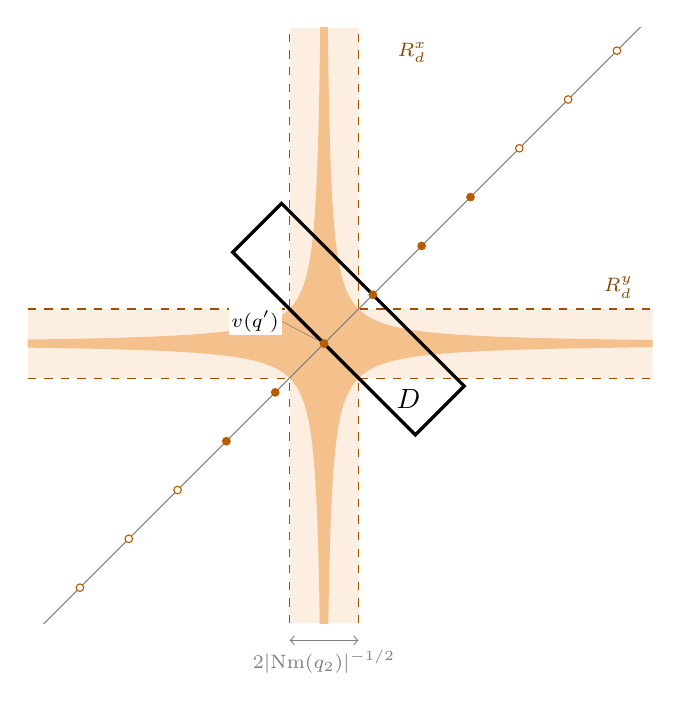
\begin{tikzpicture}[scale=0.62]
\begin{scope}\clip (-4.2,-7.6) rectangle (8.6,4.6);
\fill[regB!12] (1.1637,-7.6) rectangle (2.5779,4.6);
\fill[regB!12] (-4.2,-2.5779) rectangle (8.6,-1.1637);
\draw[regB!70!black, dashed, thin] (1.1637,-7.6) -- (1.1637,4.6) (2.5779,-7.6) -- (2.5779,4.6);
\draw[regB!70!black, dashed, thin] (-4.2,-2.5779) -- (8.6,-2.5779) (-4.2,-1.1637) -- (8.6,-1.1637);
\fill[regB!45] (41.8708,-1.8583) -- (36.8364,-1.8565) -- (32.4356,-1.8545) -- (28.5887,-1.8521) -- (25.226,-1.8494) -- (22.2865,-1.8463) -- (19.717,-1.8428) -- (17.4709,-1.8388) -- (15.5074,-1.8342) -- (13.7911,-1.8289) -- (12.2908,-1.8228) -- (10.9794,-1.8159) -- (9.833,-1.808) -- (8.8309,-1.799) -- (7.9549,-1.7886) -- (7.1891,-1.7768) -- (6.5198,-1.7633) -- (5.9346,-1.7478) -- (5.4232,-1.7301) -- (4.9761,-1.7098) -- (4.5852,-1.6866) -- (4.2436,-1.6601) -- (3.945,-1.6298) -- (3.6839,-1.5951) -- (3.4557,-1.5554) -- (3.2562,-1.5099) -- (3.0819,-1.458) -- (2.9295,-1.3985) -- (2.7962,-1.3305) -- (2.6797,-1.2527) -- (2.5779,-1.1637) -- (2.4889,-1.0619) -- (2.4111,-0.9454) -- (2.3431,-0.8122) -- (2.2837,-0.6598) -- (2.2317,-0.4854) -- (2.1863,-0.2859) -- (2.1466,-0.0577) -- (2.1119,0.2033) -- (2.0816,0.502) -- (2.055,0.8436) -- (2.0318,1.2344) -- (2.0116,1.6815) -- (1.9939,2.193) -- (1.9784,2.7781) -- (1.9648,3.4475) -- (1.953,4.2132) -- (1.9427,5.0892) -- (1.9336,6.0913) -- (1.9257,7.2377) -- (1.9188,8.5492) -- (1.9128,10.0495) -- (1.9075,11.7658) -- (1.9029,13.7292) -- (1.8988,15.9753) -- (1.8953,18.5449) -- (1.8922,21.4844) -- (1.8895,24.8471) -- (1.8872,28.694) -- (1.8851,33.0948) -- (1.8833,38.1292) -- (1.8583,38.1292) -- (1.8565,33.0948) -- (1.8545,28.694) -- (1.8521,24.8471) -- (1.8494,21.4844) -- (1.8463,18.5449) -- (1.8428,15.9753) -- (1.8388,13.7292) -- (1.8342,11.7658) -- (1.8289,10.0495) -- (1.8228,8.5492) -- (1.8159,7.2377) -- (1.808,6.0913) -- (1.799,5.0892) -- (1.7886,4.2132) -- (1.7768,3.4475) -- (1.7633,2.7781) -- (1.7478,2.193) -- (1.7301,1.6815) -- (1.7098,1.2344) -- (1.6866,0.8436) -- (1.6601,0.502) -- (1.6298,0.2033) -- (1.5951,-0.0577) -- (1.5554,-0.2859) -- (1.5099,-0.4854) -- (1.458,-0.6598) -- (1.3985,-0.8122) -- (1.3305,-0.9454) -- (1.2527,-1.0619) -- (1.1637,-1.1637) -- (1.0619,-1.2527) -- (0.9454,-1.3305) -- (0.8122,-1.3985) -- (0.6598,-1.458) -- (0.4854,-1.5099) -- (0.2859,-1.5554) -- (0.0577,-1.5951) -- (-0.2033,-1.6298) -- (-0.502,-1.6601) -- (-0.8436,-1.6866) -- (-1.2344,-1.7098) -- (-1.6815,-1.7301) -- (-2.193,-1.7478) -- (-2.7781,-1.7633) -- (-3.4475,-1.7768) -- (-4.2132,-1.7886) -- (-5.0892,-1.799) -- (-6.0913,-1.808) -- (-7.2377,-1.8159) -- (-8.5492,-1.8228) -- (-10.0495,-1.8289) -- (-11.7658,-1.8342) -- (-13.7292,-1.8388) -- (-15.9753,-1.8428) -- (-18.5449,-1.8463) -- (-21.4844,-1.8494) -- (-24.8471,-1.8521) -- (-28.694,-1.8545) -- (-33.0948,-1.8565) -- (-38.1292,-1.8583) -- (-38.1292,-1.8833) -- (-33.0948,-1.8851) -- (-28.694,-1.8872) -- (-24.8471,-1.8895) -- (-21.4844,-1.8922) -- (-18.5449,-1.8953) -- (-15.9753,-1.8988) -- (-13.7292,-1.9029) -- (-11.7658,-1.9075) -- (-10.0495,-1.9128) -- (-8.5492,-1.9188) -- (-7.2377,-1.9257) -- (-6.0913,-1.9336) -- (-5.0892,-1.9427) -- (-4.2132,-1.953) -- (-3.4475,-1.9648) -- (-2.7781,-1.9784) -- (-2.193,-1.9939) -- (-1.6815,-2.0116) -- (-1.2344,-2.0318) -- (-0.8436,-2.055) -- (-0.502,-2.0816) -- (-0.2033,-2.1119) -- (0.0577,-2.1466) -- (0.2859,-2.1863) -- (0.4854,-2.2317) -- (0.6598,-2.2837) -- (0.8122,-2.3431) -- (0.9454,-2.4111) -- (1.0619,-2.4889) -- (1.1637,-2.5779) -- (1.2527,-2.6797) -- (1.3305,-2.7962) -- (1.3985,-2.9295) -- (1.458,-3.0819) -- (1.5099,-3.2562) -- (1.5554,-3.4557) -- (1.5951,-3.6839) -- (1.6298,-3.945) -- (1.6601,-4.2436) -- (1.6866,-4.5852) -- (1.7098,-4.9761) -- (1.7301,-5.4232) -- (1.7478,-5.9346) -- (1.7633,-6.5198) -- (1.7768,-7.1891) -- (1.7886,-7.9549) -- (1.799,-8.8309) -- (1.808,-9.833) -- (1.8159,-10.9794) -- (1.8228,-12.2908) -- (1.8289,-13.7911) -- (1.8342,-15.5074) -- (1.8388,-17.4709) -- (1.8428,-19.717) -- (1.8463,-22.2865) -- (1.8494,-25.226) -- (1.8521,-28.5887) -- (1.8545,-32.4356) -- (1.8565,-36.8364) -- (1.8583,-41.8708) -- (1.8833,-41.8708) -- (1.8851,-36.8364) -- (1.8872,-32.4356) -- (1.8895,-28.5887) -- (1.8922,-25.226) -- (1.8953,-22.2865) -- (1.8988,-19.717) -- (1.9029,-17.4709) -- (1.9075,-15.5074) -- (1.9128,-13.7911) -- (1.9188,-12.2908) -- (1.9257,-10.9794) -- (1.9336,-9.833) -- (1.9427,-8.8309) -- (1.953,-7.9549) -- (1.9648,-7.1891) -- (1.9784,-6.5198) -- (1.9939,-5.9346) -- (2.0116,-5.4232) -- (2.0318,-4.9761) -- (2.055,-4.5852) -- (2.0816,-4.2436) -- (2.1119,-3.945) -- (2.1466,-3.6839) -- (2.1863,-3.4557) -- (2.2317,-3.2562) -- (2.2837,-3.0819) -- (2.3431,-2.9295) -- (2.4111,-2.7962) -- (2.4889,-2.6797) -- (2.5779,-2.5779) -- (2.6797,-2.4889) -- (2.7962,-2.4111) -- (2.9295,-2.3431) -- (3.0819,-2.2837) -- (3.2562,-2.2317) -- (3.4557,-2.1863) -- (3.6839,-2.1466) -- (3.945,-2.1119) -- (4.2436,-2.0816) -- (4.5852,-2.055) -- (4.9761,-2.0318) -- (5.4232,-2.0116) -- (5.9346,-1.9939) -- (6.5198,-1.9784) -- (7.1891,-1.9648) -- (7.9549,-1.953) -- (8.8309,-1.9427) -- (9.833,-1.9336) -- (10.9794,-1.9257) -- (12.2908,-1.9188) -- (13.7911,-1.9128) -- (15.5074,-1.9075) -- (17.4709,-1.9029) -- (19.717,-1.8988) -- (22.2865,-1.8953) -- (25.226,-1.8922) -- (28.5887,-1.8895) -- (32.4356,-1.8872) -- (36.8364,-1.8851) -- (41.8708,-1.8833) -- cycle;
\draw[gray, thin] (-10.1292,-13.8708) -- (13.8708,10.1292);
\end{scope}
\draw[very thick] (0,0) -- (1,1) -- (4.7417,-2.7417) -- (3.7417,-3.7417) -- cycle;
\node at (3.6,-3) {$D$};
\draw[regB!80!black, fill=white] (-3.1292,-6.8708) circle (2.2pt);
\draw[regB!80!black, fill=white] (-2.1292,-5.8708) circle (2.2pt);
\draw[regB!80!black, fill=white] (-1.1292,-4.8708) circle (2.2pt);
\draw[regB!80!black, fill=regB!80!black] (-0.1292,-3.8708) circle (2.2pt);
\draw[regB!80!black, fill=regB!80!black] (0.8708,-2.8708) circle (2.2pt);
\draw[regB!80!black, fill=regB!80!black] (1.8708,-1.8708) circle (2.2pt);
\draw[regB!80!black, fill=regB!80!black] (2.8708,-0.8708) circle (2.2pt);
\draw[regB!80!black, fill=regB!80!black] (3.8708,0.1292) circle (2.2pt);
\draw[regB!80!black, fill=regB!80!black] (4.8708,1.1292) circle (2.2pt);
\draw[regB!80!black, fill=white] (5.8708,2.1292) circle (2.2pt);
\draw[regB!80!black, fill=white] (6.8708,3.1292) circle (2.2pt);
\draw[regB!80!black, fill=white] (7.8708,4.1292) circle (2.2pt);
\node[font=\scriptsize, fill=white, inner sep=1pt, anchor=east] at (1.0137,-1.4208) {$v(q')$};
\draw[gray, very thin] (1.0137,-1.4208) -- (1.8708,-1.8708);
\node[font=\scriptsize, regB!60!black] at (3.6779,4.1) {$R^x_d$};
\node[font=\scriptsize, regB!60!black] at (7.9,-0.7137) {$R^y_d$};
\draw[gray, <->] (1.1637,-7.95) -- node[below, font=\scriptsize] {$2|\mathrm{Nm}(q_2)|^{-1/2}$} (2.5779,-7.95);
\end{tikzpicture}

\caption{Finiteness of $Q_{T,N}$ for $F=\Q(\sqrt{14})$: the centres $q'=\frac{\omega}{2}+d$,
$d\in\Z$ (denominator of norm $2$) lie on a line of slope one. For $d=0$ the region $V(q')$
(dark) lies in the union of the strips $R^x_d$ and $R^y_d$. Filled dots: translates whose strips
meet $D$; open dots: $V(q')\cap D=\emptyset$.}
\label{fig:q-strips}
\end{figure}

\subsection{Certification} A box $R=[x_0,x_1]\times[y_0,y_1]$ lies in $V(q)$ if and only if its
four corners do: after moving the centre to the origin, $\max_R|xy|$ is the product of
$\max|x|$ and $\max|y|$, which is attained at a corner \cite[Lemma~3.2]{GM}. Each inclusion is
therefore decided by evaluating the norm form at four points, exactly or in interval arithmetic
(Figure~\ref{fig:q-box}).

\begin{figure}[ht]
\centering
% generated by gen_figures.py (F = Q(sqrt 14)); do not edit by hand
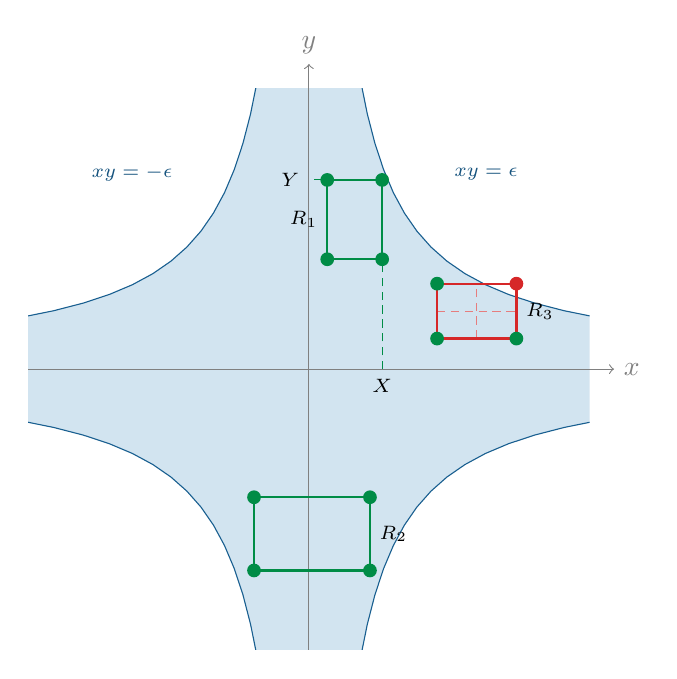
\begin{tikzpicture}[scale=1.55]
\begin{scope}\clip (-2.3,-2.3) rectangle (2.3,2.3);
\fill[regA!20] (40,0.025) -- (35.3719,0.0283) -- (31.2792,0.032) -- (27.6601,0.0362) -- (24.4597,0.0409) -- (21.6297,0.0462) -- (19.127,0.0523) -- (16.914,0.0591) -- (14.957,0.0669) -- (13.2264,0.0756) -- (11.6961,0.0855) -- (10.3428,0.0967) -- (9.1461,0.1093) -- (8.0879,0.1236) -- (7.1521,0.1398) -- (6.3246,0.1581) -- (5.5928,0.1788) -- (4.9457,0.2022) -- (4.3734,0.2287) -- (3.8674,0.2586) -- (3.42,0.2924) -- (3.0243,0.3307) -- (2.6743,0.3739) -- (2.3649,0.4228) -- (2.0913,0.4782) -- (1.8493,0.5407) -- (1.6353,0.6115) -- (1.4461,0.6915) -- (1.2788,0.782) -- (1.1308,0.8843) -- (1,1) -- (0.8843,1.1308) -- (0.782,1.2788) -- (0.6915,1.4461) -- (0.6115,1.6353) -- (0.5407,1.8493) -- (0.4782,2.0913) -- (0.4228,2.3649) -- (0.3739,2.6743) -- (0.3307,3.0243) -- (0.2924,3.42) -- (0.2586,3.8674) -- (0.2287,4.3734) -- (0.2022,4.9457) -- (0.1788,5.5928) -- (0.1581,6.3246) -- (0.1398,7.1521) -- (0.1236,8.0879) -- (0.1093,9.1461) -- (0.0967,10.3428) -- (0.0855,11.6961) -- (0.0756,13.2264) -- (0.0669,14.957) -- (0.0591,16.914) -- (0.0523,19.127) -- (0.0462,21.6297) -- (0.0409,24.4597) -- (0.0362,27.6601) -- (0.032,31.2792) -- (0.0283,35.3719) -- (0.025,40) -- (-0.025,40) -- (-0.0283,35.3719) -- (-0.032,31.2792) -- (-0.0362,27.6601) -- (-0.0409,24.4597) -- (-0.0462,21.6297) -- (-0.0523,19.127) -- (-0.0591,16.914) -- (-0.0669,14.957) -- (-0.0756,13.2264) -- (-0.0855,11.6961) -- (-0.0967,10.3428) -- (-0.1093,9.1461) -- (-0.1236,8.0879) -- (-0.1398,7.1521) -- (-0.1581,6.3246) -- (-0.1788,5.5928) -- (-0.2022,4.9457) -- (-0.2287,4.3734) -- (-0.2586,3.8674) -- (-0.2924,3.42) -- (-0.3307,3.0243) -- (-0.3739,2.6743) -- (-0.4228,2.3649) -- (-0.4782,2.0913) -- (-0.5407,1.8493) -- (-0.6115,1.6353) -- (-0.6915,1.4461) -- (-0.782,1.2788) -- (-0.8843,1.1308) -- (-1,1) -- (-1.1308,0.8843) -- (-1.2788,0.782) -- (-1.4461,0.6915) -- (-1.6353,0.6115) -- (-1.8493,0.5407) -- (-2.0913,0.4782) -- (-2.3649,0.4228) -- (-2.6743,0.3739) -- (-3.0243,0.3307) -- (-3.42,0.2924) -- (-3.8674,0.2586) -- (-4.3734,0.2287) -- (-4.9457,0.2022) -- (-5.5928,0.1788) -- (-6.3246,0.1581) -- (-7.1521,0.1398) -- (-8.0879,0.1236) -- (-9.1461,0.1093) -- (-10.3428,0.0967) -- (-11.6961,0.0855) -- (-13.2264,0.0756) -- (-14.957,0.0669) -- (-16.914,0.0591) -- (-19.127,0.0523) -- (-21.6297,0.0462) -- (-24.4597,0.0409) -- (-27.6601,0.0362) -- (-31.2792,0.032) -- (-35.3719,0.0283) -- (-40,0.025) -- (-40,-0.025) -- (-35.3719,-0.0283) -- (-31.2792,-0.032) -- (-27.6601,-0.0362) -- (-24.4597,-0.0409) -- (-21.6297,-0.0462) -- (-19.127,-0.0523) -- (-16.914,-0.0591) -- (-14.957,-0.0669) -- (-13.2264,-0.0756) -- (-11.6961,-0.0855) -- (-10.3428,-0.0967) -- (-9.1461,-0.1093) -- (-8.0879,-0.1236) -- (-7.1521,-0.1398) -- (-6.3246,-0.1581) -- (-5.5928,-0.1788) -- (-4.9457,-0.2022) -- (-4.3734,-0.2287) -- (-3.8674,-0.2586) -- (-3.42,-0.2924) -- (-3.0243,-0.3307) -- (-2.6743,-0.3739) -- (-2.3649,-0.4228) -- (-2.0913,-0.4782) -- (-1.8493,-0.5407) -- (-1.6353,-0.6115) -- (-1.4461,-0.6915) -- (-1.2788,-0.782) -- (-1.1308,-0.8843) -- (-1,-1) -- (-0.8843,-1.1308) -- (-0.782,-1.2788) -- (-0.6915,-1.4461) -- (-0.6115,-1.6353) -- (-0.5407,-1.8493) -- (-0.4782,-2.0913) -- (-0.4228,-2.3649) -- (-0.3739,-2.6743) -- (-0.3307,-3.0243) -- (-0.2924,-3.42) -- (-0.2586,-3.8674) -- (-0.2287,-4.3734) -- (-0.2022,-4.9457) -- (-0.1788,-5.5928) -- (-0.1581,-6.3246) -- (-0.1398,-7.1521) -- (-0.1236,-8.0879) -- (-0.1093,-9.1461) -- (-0.0967,-10.3428) -- (-0.0855,-11.6961) -- (-0.0756,-13.2264) -- (-0.0669,-14.957) -- (-0.0591,-16.914) -- (-0.0523,-19.127) -- (-0.0462,-21.6297) -- (-0.0409,-24.4597) -- (-0.0362,-27.6601) -- (-0.032,-31.2792) -- (-0.0283,-35.3719) -- (-0.025,-40) -- (0.025,-40) -- (0.0283,-35.3719) -- (0.032,-31.2792) -- (0.0362,-27.6601) -- (0.0409,-24.4597) -- (0.0462,-21.6297) -- (0.0523,-19.127) -- (0.0591,-16.914) -- (0.0669,-14.957) -- (0.0756,-13.2264) -- (0.0855,-11.6961) -- (0.0967,-10.3428) -- (0.1093,-9.1461) -- (0.1236,-8.0879) -- (0.1398,-7.1521) -- (0.1581,-6.3246) -- (0.1788,-5.5928) -- (0.2022,-4.9457) -- (0.2287,-4.3734) -- (0.2586,-3.8674) -- (0.2924,-3.42) -- (0.3307,-3.0243) -- (0.3739,-2.6743) -- (0.4228,-2.3649) -- (0.4782,-2.0913) -- (0.5407,-1.8493) -- (0.6115,-1.6353) -- (0.6915,-1.4461) -- (0.782,-1.2788) -- (0.8843,-1.1308) -- (1,-1) -- (1.1308,-0.8843) -- (1.2788,-0.782) -- (1.4461,-0.6915) -- (1.6353,-0.6115) -- (1.8493,-0.5407) -- (2.0913,-0.4782) -- (2.3649,-0.4228) -- (2.6743,-0.3739) -- (3.0243,-0.3307) -- (3.42,-0.2924) -- (3.8674,-0.2586) -- (4.3734,-0.2287) -- (4.9457,-0.2022) -- (5.5928,-0.1788) -- (6.3246,-0.1581) -- (7.1521,-0.1398) -- (8.0879,-0.1236) -- (9.1461,-0.1093) -- (10.3428,-0.0967) -- (11.6961,-0.0855) -- (13.2264,-0.0756) -- (14.957,-0.0669) -- (16.914,-0.0591) -- (19.127,-0.0523) -- (21.6297,-0.0462) -- (24.4597,-0.0409) -- (27.6601,-0.0362) -- (31.2792,-0.032) -- (35.3719,-0.0283) -- (40,-0.025) -- cycle;
\draw[regA!80!black, thin] (0.025,40) -- (0.0283,35.3719) -- (0.032,31.2792) -- (0.0362,27.6601) -- (0.0409,24.4597) -- (0.0462,21.6297) -- (0.0523,19.127) -- (0.0591,16.914) -- (0.0669,14.957) -- (0.0756,13.2264) -- (0.0855,11.6961) -- (0.0967,10.3428) -- (0.1093,9.1461) -- (0.1236,8.0879) -- (0.1398,7.1521) -- (0.1581,6.3246) -- (0.1788,5.5928) -- (0.2022,4.9457) -- (0.2287,4.3734) -- (0.2586,3.8674) -- (0.2924,3.42) -- (0.3307,3.0243) -- (0.3739,2.6743) -- (0.4228,2.3649) -- (0.4782,2.0913) -- (0.5407,1.8493) -- (0.6115,1.6353) -- (0.6915,1.4461) -- (0.782,1.2788) -- (0.8843,1.1308) -- (1,1) -- (1.1308,0.8843) -- (1.2788,0.782) -- (1.4461,0.6915) -- (1.6353,0.6115) -- (1.8493,0.5407) -- (2.0913,0.4782) -- (2.3649,0.4228) -- (2.6743,0.3739) -- (3.0243,0.3307) -- (3.42,0.2924) -- (3.8674,0.2586) -- (4.3734,0.2287) -- (4.9457,0.2022) -- (5.5928,0.1788) -- (6.3246,0.1581) -- (7.1521,0.1398) -- (8.0879,0.1236) -- (9.1461,0.1093) -- (10.3428,0.0967) -- (11.6961,0.0855) -- (13.2264,0.0756) -- (14.957,0.0669) -- (16.914,0.0591) -- (19.127,0.0523) -- (21.6297,0.0462) -- (24.4597,0.0409) -- (27.6601,0.0362) -- (31.2792,0.032) -- (35.3719,0.0283) -- (40,0.025);
\draw[regA!80!black, thin] (-0.025,40) -- (-0.0283,35.3719) -- (-0.032,31.2792) -- (-0.0362,27.6601) -- (-0.0409,24.4597) -- (-0.0462,21.6297) -- (-0.0523,19.127) -- (-0.0591,16.914) -- (-0.0669,14.957) -- (-0.0756,13.2264) -- (-0.0855,11.6961) -- (-0.0967,10.3428) -- (-0.1093,9.1461) -- (-0.1236,8.0879) -- (-0.1398,7.1521) -- (-0.1581,6.3246) -- (-0.1788,5.5928) -- (-0.2022,4.9457) -- (-0.2287,4.3734) -- (-0.2586,3.8674) -- (-0.2924,3.42) -- (-0.3307,3.0243) -- (-0.3739,2.6743) -- (-0.4228,2.3649) -- (-0.4782,2.0913) -- (-0.5407,1.8493) -- (-0.6115,1.6353) -- (-0.6915,1.4461) -- (-0.782,1.2788) -- (-0.8843,1.1308) -- (-1,1) -- (-1.1308,0.8843) -- (-1.2788,0.782) -- (-1.4461,0.6915) -- (-1.6353,0.6115) -- (-1.8493,0.5407) -- (-2.0913,0.4782) -- (-2.3649,0.4228) -- (-2.6743,0.3739) -- (-3.0243,0.3307) -- (-3.42,0.2924) -- (-3.8674,0.2586) -- (-4.3734,0.2287) -- (-4.9457,0.2022) -- (-5.5928,0.1788) -- (-6.3246,0.1581) -- (-7.1521,0.1398) -- (-8.0879,0.1236) -- (-9.1461,0.1093) -- (-10.3428,0.0967) -- (-11.6961,0.0855) -- (-13.2264,0.0756) -- (-14.957,0.0669) -- (-16.914,0.0591) -- (-19.127,0.0523) -- (-21.6297,0.0462) -- (-24.4597,0.0409) -- (-27.6601,0.0362) -- (-31.2792,0.032) -- (-35.3719,0.0283) -- (-40,0.025);
\draw[regA!80!black, thin] (-0.025,-40) -- (-0.0283,-35.3719) -- (-0.032,-31.2792) -- (-0.0362,-27.6601) -- (-0.0409,-24.4597) -- (-0.0462,-21.6297) -- (-0.0523,-19.127) -- (-0.0591,-16.914) -- (-0.0669,-14.957) -- (-0.0756,-13.2264) -- (-0.0855,-11.6961) -- (-0.0967,-10.3428) -- (-0.1093,-9.1461) -- (-0.1236,-8.0879) -- (-0.1398,-7.1521) -- (-0.1581,-6.3246) -- (-0.1788,-5.5928) -- (-0.2022,-4.9457) -- (-0.2287,-4.3734) -- (-0.2586,-3.8674) -- (-0.2924,-3.42) -- (-0.3307,-3.0243) -- (-0.3739,-2.6743) -- (-0.4228,-2.3649) -- (-0.4782,-2.0913) -- (-0.5407,-1.8493) -- (-0.6115,-1.6353) -- (-0.6915,-1.4461) -- (-0.782,-1.2788) -- (-0.8843,-1.1308) -- (-1,-1) -- (-1.1308,-0.8843) -- (-1.2788,-0.782) -- (-1.4461,-0.6915) -- (-1.6353,-0.6115) -- (-1.8493,-0.5407) -- (-2.0913,-0.4782) -- (-2.3649,-0.4228) -- (-2.6743,-0.3739) -- (-3.0243,-0.3307) -- (-3.42,-0.2924) -- (-3.8674,-0.2586) -- (-4.3734,-0.2287) -- (-4.9457,-0.2022) -- (-5.5928,-0.1788) -- (-6.3246,-0.1581) -- (-7.1521,-0.1398) -- (-8.0879,-0.1236) -- (-9.1461,-0.1093) -- (-10.3428,-0.0967) -- (-11.6961,-0.0855) -- (-13.2264,-0.0756) -- (-14.957,-0.0669) -- (-16.914,-0.0591) -- (-19.127,-0.0523) -- (-21.6297,-0.0462) -- (-24.4597,-0.0409) -- (-27.6601,-0.0362) -- (-31.2792,-0.032) -- (-35.3719,-0.0283) -- (-40,-0.025);
\draw[regA!80!black, thin] (0.025,-40) -- (0.0283,-35.3719) -- (0.032,-31.2792) -- (0.0362,-27.6601) -- (0.0409,-24.4597) -- (0.0462,-21.6297) -- (0.0523,-19.127) -- (0.0591,-16.914) -- (0.0669,-14.957) -- (0.0756,-13.2264) -- (0.0855,-11.6961) -- (0.0967,-10.3428) -- (0.1093,-9.1461) -- (0.1236,-8.0879) -- (0.1398,-7.1521) -- (0.1581,-6.3246) -- (0.1788,-5.5928) -- (0.2022,-4.9457) -- (0.2287,-4.3734) -- (0.2586,-3.8674) -- (0.2924,-3.42) -- (0.3307,-3.0243) -- (0.3739,-2.6743) -- (0.4228,-2.3649) -- (0.4782,-2.0913) -- (0.5407,-1.8493) -- (0.6115,-1.6353) -- (0.6915,-1.4461) -- (0.782,-1.2788) -- (0.8843,-1.1308) -- (1,-1) -- (1.1308,-0.8843) -- (1.2788,-0.782) -- (1.4461,-0.6915) -- (1.6353,-0.6115) -- (1.8493,-0.5407) -- (2.0913,-0.4782) -- (2.3649,-0.4228) -- (2.6743,-0.3739) -- (3.0243,-0.3307) -- (3.42,-0.2924) -- (3.8674,-0.2586) -- (4.3734,-0.2287) -- (4.9457,-0.2022) -- (5.5928,-0.1788) -- (6.3246,-0.1581) -- (7.1521,-0.1398) -- (8.0879,-0.1236) -- (9.1461,-0.1093) -- (10.3428,-0.0967) -- (11.6961,-0.0855) -- (13.2264,-0.0756) -- (14.957,-0.0669) -- (16.914,-0.0591) -- (19.127,-0.0523) -- (21.6297,-0.0462) -- (24.4597,-0.0409) -- (27.6601,-0.0362) -- (31.2792,-0.032) -- (35.3719,-0.0283) -- (40,-0.025);
\end{scope}
\draw[->, gray] (-2.3,0) -- (2.5,0) node[right] {$x$};
\draw[->, gray] (0,-2.3) -- (0,2.5) node[above] {$y$};
\node[regA!70!black, font=\scriptsize] at (1.45,1.6) {$xy=\epsilon$};
\node[regA!70!black, font=\scriptsize] at (-1.45,1.6) {$xy=-\epsilon$};
\draw[thick, good] (0.15,0.9) rectangle (0.6,1.55);
\fill[good] (0.15,0.9) circle (1.6pt);
\fill[good] (0.15,1.55) circle (1.6pt);
\fill[good] (0.6,0.9) circle (1.6pt);
\fill[good] (0.6,1.55) circle (1.6pt);
\node[font=\scriptsize, left] at (0.15,1.225) {$R_1$};
\draw[good, densely dashed] (0.6,0) -- (0.6,1.55) -- (0,1.55);
\node[font=\scriptsize, below] at (0.6,0) {$X$};
\node[font=\scriptsize, left] at (0,1.55) {$Y$};
\draw[thick, good] (-0.45,-1.65) rectangle (0.5,-1.05);
\fill[good] (-0.45,-1.65) circle (1.6pt);
\fill[good] (-0.45,-1.05) circle (1.6pt);
\fill[good] (0.5,-1.65) circle (1.6pt);
\fill[good] (0.5,-1.05) circle (1.6pt);
\node[font=\scriptsize, right] at (0.5,-1.35) {$R_2$};
\draw[bad!60, densely dashed] (1.375,0.25) -- (1.375,0.7) (1.05,0.475) -- (1.7,0.475);
\draw[thick, bad] (1.05,0.25) rectangle (1.7,0.7);
\fill[good] (1.05,0.25) circle (1.6pt);
\fill[good] (1.05,0.7) circle (1.6pt);
\fill[good] (1.7,0.25) circle (1.6pt);
\fill[bad] (1.7,0.7) circle (1.6pt);
\node[font=\scriptsize, right] at (1.7,0.475) {$R_3$};
\end{tikzpicture}

\caption{The corner test for $V(q)=\{|xy|<\epsilon\}$. Green (red) dots are corners inside
(outside) $V(q)$. All corners of $R_1$ lie in $V(q)$, so $R_1\subset V(q)$, since $|x|\le X$,
$|y|\le Y$ on $R_1$ and $XY<\epsilon$. The same holds for $R_2$, although it meets $x=0$. The
box $R_3$ is rejected and subdivided into four boxes (dashed), three of which pass the test.}
\label{fig:q-box}
\end{figure}

\subsection{The algorithm} \textbf{SOLVE} receives a box $R$, starting with a box $R_0\supset D$.
If some $q\in Q_{T,N}$ has $R\subset V(q)$ it records the pair, and otherwise it subdivides $R$
into four boxes and recurses, increasing $T$ and $N$ with the depth. It terminates if and
only if $F$ is $2$-stage Euclidean \cite[Theorem~3.4]{GM} (the proof there uses the
equivalence above), and the recorded pairs form a certificate from which continued fractions
are computed. Figures~\ref{fig:q-solve} and~\ref{fig:q-zoom} show
it for $\Q(\sqrt{14})$, with $T=3$ and $N$ fixed. With $N=1$ the subdivision cannot end, because
some points of $D$ lie in no region with unit denominator. With $N=2$ it returns $124$ boxes
covered by $22$ regions. Some of their centres lie far from $D$, such as $v(-8-2\omega)\approx
(-15.5,-0.5)$, and reach it through a thin arm.

\begin{figure}[ht]
\centering
% generated by gen_figures.py (F = Q(sqrt 14)); do not edit by hand
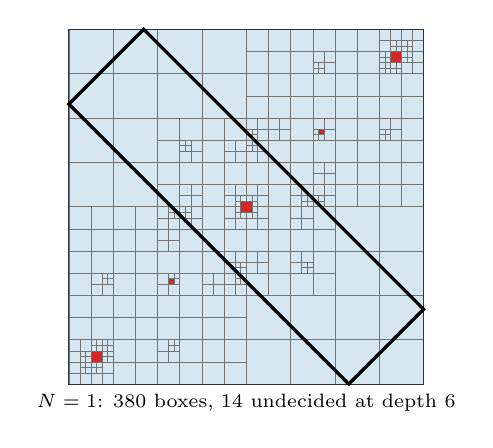
\begin{tikzpicture}[scale=0.95]
\fill[regA!18] (4.594,0.8518) rectangle (4.7422,1);
\fill[regA!18] (4.4458,0.8518) rectangle (4.594,1);
\fill[regA!18] (4.594,0.7036) rectangle (4.7422,0.8518);
\fill[regA!18] (4.5199,0.7777) rectangle (4.594,0.8518);
\fill[regA!18] (4.4458,0.7777) rectangle (4.5199,0.8518);
\fill[regA!18] (4.5199,0.7036) rectangle (4.594,0.7777);
\fill[regA!18] (4.4458,0.7036) rectangle (4.5199,0.7777);
\fill[regA!18] (4.2976,0.8518) rectangle (4.4458,1);
\fill[regA!18] (4.1494,0.8518) rectangle (4.2976,1);
\fill[regA!18] (4.3717,0.7777) rectangle (4.4458,0.8518);
\fill[regA!18] (4.2976,0.7777) rectangle (4.3717,0.8518);
\fill[regA!18] (4.3717,0.7036) rectangle (4.4458,0.7777);
\fill[regA!18] (4.2976,0.7036) rectangle (4.3717,0.7777);
\fill[regA!18] (4.1494,0.7036) rectangle (4.2976,0.8518);
\fill[regA!18] (4.594,0.5554) rectangle (4.7422,0.7036);
\fill[regA!18] (4.5199,0.6295) rectangle (4.594,0.7036);
\fill[regA!18] (4.4458,0.6295) rectangle (4.5199,0.7036);
\fill[regA!18] (4.5199,0.5554) rectangle (4.594,0.6295);
\fill[regA!18] (4.4458,0.5554) rectangle (4.5199,0.6295);
\fill[regA!18] (4.594,0.4072) rectangle (4.7422,0.5554);
\fill[regA!18] (4.4458,0.4072) rectangle (4.594,0.5554);
\fill[regA!18] (4.2235,0.6295) rectangle (4.2976,0.7036);
\fill[regA!18] (4.1494,0.6295) rectangle (4.2235,0.7036);
\fill[regA!18] (4.2235,0.5554) rectangle (4.2976,0.6295);
\fill[regA!18] (4.1494,0.5554) rectangle (4.2235,0.6295);
\fill[regA!18] (4.3717,0.4813) rectangle (4.4458,0.5554);
\fill[regA!18] (4.2976,0.4813) rectangle (4.3717,0.5554);
\fill[regA!18] (4.3717,0.4072) rectangle (4.4458,0.4813);
\fill[regA!18] (4.2976,0.4072) rectangle (4.3717,0.4813);
\fill[regA!18] (4.2235,0.4813) rectangle (4.2976,0.5554);
\fill[regA!18] (4.1494,0.4813) rectangle (4.2235,0.5554);
\fill[regA!18] (4.2235,0.4072) rectangle (4.2976,0.4813);
\fill[regA!18] (4.1494,0.4072) rectangle (4.2235,0.4813);
\fill[regA!18] (3.853,0.7036) rectangle (4.1494,1);
\fill[regA!18] (3.5566,0.7036) rectangle (3.853,1);
\fill[regA!18] (3.853,0.4072) rectangle (4.1494,0.7036);
\fill[regA!18] (3.5566,0.4072) rectangle (3.853,0.7036);
\fill[regA!18] (4.4458,0.1108) rectangle (4.7422,0.4072);
\fill[regA!18] (4.1494,0.1108) rectangle (4.4458,0.4072);
\fill[regA!18] (4.4458,-0.1855) rectangle (4.7422,0.1108);
\fill[regA!18] (4.1494,-0.1855) rectangle (4.4458,0.1108);
\fill[regA!18] (3.853,0.1108) rectangle (4.1494,0.4072);
\fill[regA!18] (3.5566,0.1108) rectangle (3.853,0.4072);
\fill[regA!18] (3.853,-0.1855) rectangle (4.1494,0.1108);
\fill[regA!18] (3.5566,-0.1855) rectangle (3.853,0.1108);
\fill[regA!18] (3.2603,0.7036) rectangle (3.5566,1);
\fill[regA!18] (2.9639,0.7036) rectangle (3.2603,1);
\fill[regA!18] (3.4084,0.5554) rectangle (3.5566,0.7036);
\fill[regA!18] (3.2603,0.5554) rectangle (3.4084,0.7036);
\fill[regA!18] (3.4084,0.4072) rectangle (3.5566,0.5554);
\fill[regA!18] (3.3344,0.4813) rectangle (3.4084,0.5554);
\fill[regA!18] (3.2603,0.4813) rectangle (3.3344,0.5554);
\fill[regA!18] (3.3344,0.4072) rectangle (3.4084,0.4813);
\fill[regA!18] (3.2603,0.4072) rectangle (3.3344,0.4813);
\fill[regA!18] (2.9639,0.4072) rectangle (3.2603,0.7036);
\fill[regA!18] (2.6675,0.7036) rectangle (2.9639,1);
\fill[regA!18] (2.3711,0.7036) rectangle (2.6675,1);
\fill[regA!18] (2.6675,0.4072) rectangle (2.9639,0.7036);
\fill[regA!18] (2.3711,0.4072) rectangle (2.6675,0.7036);
\fill[regA!18] (3.2603,0.1108) rectangle (3.5566,0.4072);
\fill[regA!18] (2.9639,0.1108) rectangle (3.2603,0.4072);
\fill[regA!18] (3.2603,-0.1855) rectangle (3.5566,0.1108);
\fill[regA!18] (2.9639,-0.1855) rectangle (3.2603,0.1108);
\fill[regA!18] (2.6675,0.1108) rectangle (2.9639,0.4072);
\fill[regA!18] (2.3711,0.1108) rectangle (2.6675,0.4072);
\fill[regA!18] (2.6675,-0.1855) rectangle (2.9639,0.1108);
\fill[regA!18] (2.3711,-0.1855) rectangle (2.6675,0.1108);
\fill[regA!18] (4.4458,-0.4819) rectangle (4.7422,-0.1855);
\fill[regA!18] (4.2976,-0.3337) rectangle (4.4458,-0.1855);
\fill[regA!18] (4.1494,-0.3337) rectangle (4.2976,-0.1855);
\fill[regA!18] (4.2976,-0.4819) rectangle (4.4458,-0.3337);
\fill[regA!18] (4.2235,-0.4078) rectangle (4.2976,-0.3337);
\fill[regA!18] (4.1494,-0.4078) rectangle (4.2235,-0.3337);
\fill[regA!18] (4.2235,-0.4819) rectangle (4.2976,-0.4078);
\fill[regA!18] (4.1494,-0.4819) rectangle (4.2235,-0.4078);
\fill[regA!18] (4.4458,-0.7783) rectangle (4.7422,-0.4819);
\fill[regA!18] (4.1494,-0.7783) rectangle (4.4458,-0.4819);
\fill[regA!18] (3.853,-0.4819) rectangle (4.1494,-0.1855);
\fill[regA!18] (3.5566,-0.4819) rectangle (3.853,-0.1855);
\fill[regA!18] (3.853,-0.7783) rectangle (4.1494,-0.4819);
\fill[regA!18] (3.5566,-0.7783) rectangle (3.853,-0.4819);
\fill[regA!18] (4.4458,-1.0747) rectangle (4.7422,-0.7783);
\fill[regA!18] (4.1494,-1.0747) rectangle (4.4458,-0.7783);
\fill[regA!18] (4.4458,-1.3711) rectangle (4.7422,-1.0747);
\fill[regA!18] (4.1494,-1.3711) rectangle (4.4458,-1.0747);
\fill[regA!18] (3.853,-1.0747) rectangle (4.1494,-0.7783);
\fill[regA!18] (3.5566,-1.0747) rectangle (3.853,-0.7783);
\fill[regA!18] (3.853,-1.3711) rectangle (4.1494,-1.0747);
\fill[regA!18] (3.5566,-1.3711) rectangle (3.853,-1.0747);
\fill[regA!18] (3.4084,-0.3337) rectangle (3.5566,-0.1855);
\fill[regA!18] (3.2603,-0.3337) rectangle (3.4084,-0.1855);
\fill[regA!18] (3.4084,-0.4819) rectangle (3.5566,-0.3337);
\fill[regA!18] (3.2603,-0.4078) rectangle (3.3344,-0.3337);
\fill[regA!18] (3.3344,-0.4819) rectangle (3.4084,-0.4078);
\fill[regA!18] (3.2603,-0.4819) rectangle (3.3344,-0.4078);
\fill[regA!18] (2.9639,-0.4819) rectangle (3.2603,-0.1855);
\fill[regA!18] (3.2603,-0.7783) rectangle (3.5566,-0.4819);
\fill[regA!18] (2.9639,-0.7783) rectangle (3.2603,-0.4819);
\fill[regA!18] (2.8157,-0.3337) rectangle (2.9639,-0.1855);
\fill[regA!18] (2.6675,-0.3337) rectangle (2.8157,-0.1855);
\fill[regA!18] (2.8157,-0.4819) rectangle (2.9639,-0.3337);
\fill[regA!18] (2.6675,-0.4819) rectangle (2.8157,-0.3337);
\fill[regA!18] (2.5193,-0.3337) rectangle (2.6675,-0.1855);
\fill[regA!18] (2.3711,-0.3337) rectangle (2.5193,-0.1855);
\fill[regA!18] (2.5193,-0.4819) rectangle (2.6675,-0.3337);
\fill[regA!18] (2.4452,-0.4078) rectangle (2.5193,-0.3337);
\fill[regA!18] (2.3711,-0.4078) rectangle (2.4452,-0.3337);
\fill[regA!18] (2.4452,-0.4819) rectangle (2.5193,-0.4078);
\fill[regA!18] (2.3711,-0.4819) rectangle (2.4452,-0.4078);
\fill[regA!18] (2.6675,-0.7783) rectangle (2.9639,-0.4819);
\fill[regA!18] (2.5193,-0.6301) rectangle (2.6675,-0.4819);
\fill[regA!18] (2.4452,-0.556) rectangle (2.5193,-0.4819);
\fill[regA!18] (2.3711,-0.556) rectangle (2.4452,-0.4819);
\fill[regA!18] (2.4452,-0.6301) rectangle (2.5193,-0.556);
\fill[regA!18] (2.3711,-0.6301) rectangle (2.4452,-0.556);
\fill[regA!18] (2.5193,-0.7783) rectangle (2.6675,-0.6301);
\fill[regA!18] (2.3711,-0.7783) rectangle (2.5193,-0.6301);
\fill[regA!18] (3.4084,-0.9265) rectangle (3.5566,-0.7783);
\fill[regA!18] (3.2603,-0.9265) rectangle (3.4084,-0.7783);
\fill[regA!18] (3.4084,-1.0747) rectangle (3.5566,-0.9265);
\fill[regA!18] (3.2603,-1.0747) rectangle (3.4084,-0.9265);
\fill[regA!18] (2.9639,-1.0747) rectangle (3.2603,-0.7783);
\fill[regA!18] (3.4084,-1.2229) rectangle (3.5566,-1.0747);
\fill[regA!18] (3.2603,-1.2229) rectangle (3.4084,-1.0747);
\fill[regA!18] (3.4084,-1.3711) rectangle (3.5566,-1.2229);
\fill[regA!18] (3.3344,-1.297) rectangle (3.4084,-1.2229);
\fill[regA!18] (3.2603,-1.297) rectangle (3.3344,-1.2229);
\fill[regA!18] (3.3344,-1.3711) rectangle (3.4084,-1.297);
\fill[regA!18] (3.2603,-1.3711) rectangle (3.3344,-1.297);
\fill[regA!18] (3.1121,-1.2229) rectangle (3.2603,-1.0747);
\fill[regA!18] (2.9639,-1.2229) rectangle (3.1121,-1.0747);
\fill[regA!18] (3.1862,-1.297) rectangle (3.2603,-1.2229);
\fill[regA!18] (3.1121,-1.297) rectangle (3.1862,-1.2229);
\fill[regA!18] (3.1862,-1.3711) rectangle (3.2603,-1.297);
\fill[regA!18] (3.1121,-1.3711) rectangle (3.1862,-1.297);
\fill[regA!18] (2.9639,-1.3711) rectangle (3.1121,-1.2229);
\fill[regA!18] (2.6675,-1.0747) rectangle (2.9639,-0.7783);
\fill[regA!18] (2.3711,-1.0747) rectangle (2.6675,-0.7783);
\fill[regA!18] (2.6675,-1.3711) rectangle (2.9639,-1.0747);
\fill[regA!18] (2.5193,-1.2229) rectangle (2.6675,-1.0747);
\fill[regA!18] (2.3711,-1.2229) rectangle (2.5193,-1.0747);
\fill[regA!18] (2.5193,-1.3711) rectangle (2.6675,-1.2229);
\fill[regA!18] (2.4452,-1.297) rectangle (2.5193,-1.2229);
\fill[regA!18] (2.3711,-1.297) rectangle (2.4452,-1.2229);
\fill[regA!18] (2.4452,-1.3711) rectangle (2.5193,-1.297);
\fill[regA!18] (1.7783,0.4072) rectangle (2.3711,1);
\fill[regA!18] (1.1855,0.4072) rectangle (1.7783,1);
\fill[regA!18] (1.7783,-0.1855) rectangle (2.3711,0.4072);
\fill[regA!18] (1.1855,-0.1855) rectangle (1.7783,0.4072);
\fill[regA!18] (0.5928,0.4072) rectangle (1.1855,1);
\fill[regA!18] (0,0.4072) rectangle (0.5928,1);
\fill[regA!18] (0.5928,-0.1855) rectangle (1.1855,0.4072);
\fill[regA!18] (0,-0.1855) rectangle (0.5928,0.4072);
\fill[regA!18] (2.0747,-0.4819) rectangle (2.3711,-0.1855);
\fill[regA!18] (1.7783,-0.4819) rectangle (2.0747,-0.1855);
\fill[regA!18] (2.2229,-0.6301) rectangle (2.3711,-0.4819);
\fill[regA!18] (2.0747,-0.6301) rectangle (2.2229,-0.4819);
\fill[regA!18] (2.2229,-0.7783) rectangle (2.3711,-0.6301);
\fill[regA!18] (2.0747,-0.7783) rectangle (2.2229,-0.6301);
\fill[regA!18] (1.7783,-0.7783) rectangle (2.0747,-0.4819);
\fill[regA!18] (1.4819,-0.4819) rectangle (1.7783,-0.1855);
\fill[regA!18] (1.1855,-0.4819) rectangle (1.4819,-0.1855);
\fill[regA!18] (1.6301,-0.6301) rectangle (1.7783,-0.4819);
\fill[regA!18] (1.556,-0.556) rectangle (1.6301,-0.4819);
\fill[regA!18] (1.4819,-0.556) rectangle (1.556,-0.4819);
\fill[regA!18] (1.556,-0.6301) rectangle (1.6301,-0.556);
\fill[regA!18] (1.4819,-0.6301) rectangle (1.556,-0.556);
\fill[regA!18] (1.6301,-0.7783) rectangle (1.7783,-0.6301);
\fill[regA!18] (1.4819,-0.7783) rectangle (1.6301,-0.6301);
\fill[regA!18] (1.1855,-0.7783) rectangle (1.4819,-0.4819);
\fill[regA!18] (2.0747,-1.0747) rectangle (2.3711,-0.7783);
\fill[regA!18] (1.7783,-1.0747) rectangle (2.0747,-0.7783);
\fill[regA!18] (2.2229,-1.2229) rectangle (2.3711,-1.0747);
\fill[regA!18] (2.0747,-1.2229) rectangle (2.2229,-1.0747);
\fill[regA!18] (2.297,-1.297) rectangle (2.3711,-1.2229);
\fill[regA!18] (2.2229,-1.297) rectangle (2.297,-1.2229);
\fill[regA!18] (2.2229,-1.3711) rectangle (2.297,-1.297);
\fill[regA!18] (2.0747,-1.3711) rectangle (2.2229,-1.2229);
\fill[regA!18] (1.7783,-1.3711) rectangle (2.0747,-1.0747);
\fill[regA!18] (1.4819,-1.0747) rectangle (1.7783,-0.7783);
\fill[regA!18] (1.1855,-1.0747) rectangle (1.4819,-0.7783);
\fill[regA!18] (1.6301,-1.2229) rectangle (1.7783,-1.0747);
\fill[regA!18] (1.4819,-1.2229) rectangle (1.6301,-1.0747);
\fill[regA!18] (1.6301,-1.3711) rectangle (1.7783,-1.2229);
\fill[regA!18] (1.4819,-1.3711) rectangle (1.6301,-1.2229);
\fill[regA!18] (1.1855,-1.3711) rectangle (1.4819,-1.0747);
\fill[regA!18] (0.5928,-0.7783) rectangle (1.1855,-0.1855);
\fill[regA!18] (0,-0.7783) rectangle (0.5928,-0.1855);
\fill[regA!18] (0.5928,-1.3711) rectangle (1.1855,-0.7783);
\fill[regA!18] (0,-1.3711) rectangle (0.5928,-0.7783);
\fill[regA!18] (4.1494,-1.9639) rectangle (4.7422,-1.3711);
\fill[regA!18] (3.5566,-1.9639) rectangle (4.1494,-1.3711);
\fill[regA!18] (4.1494,-2.5566) rectangle (4.7422,-1.9639);
\fill[regA!18] (3.5566,-2.5566) rectangle (4.1494,-1.9639);
\fill[regA!18] (3.2603,-1.6675) rectangle (3.5566,-1.3711);
\fill[regA!18] (3.1121,-1.5193) rectangle (3.2603,-1.3711);
\fill[regA!18] (2.9639,-1.5193) rectangle (3.1121,-1.3711);
\fill[regA!18] (3.1121,-1.6675) rectangle (3.2603,-1.5193);
\fill[regA!18] (2.9639,-1.6675) rectangle (3.1121,-1.5193);
\fill[regA!18] (3.2603,-1.9639) rectangle (3.5566,-1.6675);
\fill[regA!18] (2.9639,-1.9639) rectangle (3.2603,-1.6675);
\fill[regA!18] (2.6675,-1.6675) rectangle (2.9639,-1.3711);
\fill[regA!18] (2.5193,-1.5193) rectangle (2.6675,-1.3711);
\fill[regA!18] (2.4452,-1.4452) rectangle (2.5193,-1.3711);
\fill[regA!18] (2.4452,-1.5193) rectangle (2.5193,-1.4452);
\fill[regA!18] (2.3711,-1.5193) rectangle (2.4452,-1.4452);
\fill[regA!18] (2.5193,-1.6675) rectangle (2.6675,-1.5193);
\fill[regA!18] (2.3711,-1.6675) rectangle (2.5193,-1.5193);
\fill[regA!18] (2.6675,-1.9639) rectangle (2.9639,-1.6675);
\fill[regA!18] (2.3711,-1.9639) rectangle (2.6675,-1.6675);
\fill[regA!18] (3.2603,-2.2603) rectangle (3.5566,-1.9639);
\fill[regA!18] (3.1121,-2.1121) rectangle (3.2603,-1.9639);
\fill[regA!18] (2.9639,-2.1121) rectangle (3.1121,-1.9639);
\fill[regA!18] (3.1862,-2.1862) rectangle (3.2603,-2.1121);
\fill[regA!18] (3.1121,-2.1862) rectangle (3.1862,-2.1121);
\fill[regA!18] (3.1862,-2.2603) rectangle (3.2603,-2.1862);
\fill[regA!18] (3.1121,-2.2603) rectangle (3.1862,-2.1862);
\fill[regA!18] (2.9639,-2.2603) rectangle (3.1121,-2.1121);
\fill[regA!18] (3.2603,-2.5566) rectangle (3.5566,-2.2603);
\fill[regA!18] (2.9639,-2.5566) rectangle (3.2603,-2.2603);
\fill[regA!18] (2.6675,-2.2603) rectangle (2.9639,-1.9639);
\fill[regA!18] (2.5193,-2.1121) rectangle (2.6675,-1.9639);
\fill[regA!18] (2.3711,-2.1121) rectangle (2.5193,-1.9639);
\fill[regA!18] (2.5193,-2.2603) rectangle (2.6675,-2.1121);
\fill[regA!18] (2.3711,-2.2603) rectangle (2.5193,-2.1121);
\fill[regA!18] (2.6675,-2.5566) rectangle (2.9639,-2.2603);
\fill[regA!18] (2.3711,-2.5566) rectangle (2.6675,-2.2603);
\fill[regA!18] (4.1494,-3.1494) rectangle (4.7422,-2.5566);
\fill[regA!18] (3.5566,-3.1494) rectangle (4.1494,-2.5566);
\fill[regA!18] (4.1494,-3.7422) rectangle (4.7422,-3.1494);
\fill[regA!18] (3.5566,-3.7422) rectangle (4.1494,-3.1494);
\fill[regA!18] (2.9639,-3.1494) rectangle (3.5566,-2.5566);
\fill[regA!18] (2.3711,-3.1494) rectangle (2.9639,-2.5566);
\fill[regA!18] (2.9639,-3.7422) rectangle (3.5566,-3.1494);
\fill[regA!18] (2.3711,-3.7422) rectangle (2.9639,-3.1494);
\fill[regA!18] (2.2229,-1.4452) rectangle (2.297,-1.3711);
\fill[regA!18] (2.297,-1.5193) rectangle (2.3711,-1.4452);
\fill[regA!18] (2.2229,-1.5193) rectangle (2.297,-1.4452);
\fill[regA!18] (2.0747,-1.5193) rectangle (2.2229,-1.3711);
\fill[regA!18] (2.2229,-1.6675) rectangle (2.3711,-1.5193);
\fill[regA!18] (2.0747,-1.6675) rectangle (2.2229,-1.5193);
\fill[regA!18] (1.7783,-1.6675) rectangle (2.0747,-1.3711);
\fill[regA!18] (2.0747,-1.9639) rectangle (2.3711,-1.6675);
\fill[regA!18] (1.7783,-1.9639) rectangle (2.0747,-1.6675);
\fill[regA!18] (1.6301,-1.5193) rectangle (1.7783,-1.3711);
\fill[regA!18] (1.556,-1.4452) rectangle (1.6301,-1.3711);
\fill[regA!18] (1.4819,-1.4452) rectangle (1.556,-1.3711);
\fill[regA!18] (1.556,-1.5193) rectangle (1.6301,-1.4452);
\fill[regA!18] (1.4819,-1.5193) rectangle (1.556,-1.4452);
\fill[regA!18] (1.6301,-1.6675) rectangle (1.7783,-1.5193);
\fill[regA!18] (1.4819,-1.6675) rectangle (1.6301,-1.5193);
\fill[regA!18] (1.4078,-1.4452) rectangle (1.4819,-1.3711);
\fill[regA!18] (1.3337,-1.4452) rectangle (1.4078,-1.3711);
\fill[regA!18] (1.4078,-1.5193) rectangle (1.4819,-1.4452);
\fill[regA!18] (1.3337,-1.5193) rectangle (1.4078,-1.4452);
\fill[regA!18] (1.1855,-1.5193) rectangle (1.3337,-1.3711);
\fill[regA!18] (1.3337,-1.6675) rectangle (1.4819,-1.5193);
\fill[regA!18] (1.1855,-1.6675) rectangle (1.3337,-1.5193);
\fill[regA!18] (1.4819,-1.9639) rectangle (1.7783,-1.6675);
\fill[regA!18] (1.3337,-1.8157) rectangle (1.4819,-1.6675);
\fill[regA!18] (1.1855,-1.8157) rectangle (1.3337,-1.6675);
\fill[regA!18] (1.3337,-1.9639) rectangle (1.4819,-1.8157);
\fill[regA!18] (1.1855,-1.9639) rectangle (1.3337,-1.8157);
\fill[regA!18] (2.2229,-2.1121) rectangle (2.3711,-1.9639);
\fill[regA!18] (2.0747,-2.1121) rectangle (2.2229,-1.9639);
\fill[regA!18] (2.297,-2.1862) rectangle (2.3711,-2.1121);
\fill[regA!18] (2.2229,-2.1862) rectangle (2.297,-2.1121);
\fill[regA!18] (2.297,-2.2603) rectangle (2.3711,-2.1862);
\fill[regA!18] (2.2229,-2.2603) rectangle (2.297,-2.1862);
\fill[regA!18] (2.0747,-2.2603) rectangle (2.2229,-2.1121);
\fill[regA!18] (1.7783,-2.2603) rectangle (2.0747,-1.9639);
\fill[regA!18] (2.297,-2.3344) rectangle (2.3711,-2.2603);
\fill[regA!18] (2.2229,-2.3344) rectangle (2.297,-2.2603);
\fill[regA!18] (2.297,-2.4084) rectangle (2.3711,-2.3344);
\fill[regA!18] (2.2229,-2.4084) rectangle (2.297,-2.3344);
\fill[regA!18] (2.0747,-2.4084) rectangle (2.2229,-2.2603);
\fill[regA!18] (2.2229,-2.5566) rectangle (2.3711,-2.4084);
\fill[regA!18] (2.0747,-2.5566) rectangle (2.2229,-2.4084);
\fill[regA!18] (1.9265,-2.4084) rectangle (2.0747,-2.2603);
\fill[regA!18] (1.7783,-2.4084) rectangle (1.9265,-2.2603);
\fill[regA!18] (1.9265,-2.5566) rectangle (2.0747,-2.4084);
\fill[regA!18] (1.7783,-2.5566) rectangle (1.9265,-2.4084);
\fill[regA!18] (1.4819,-2.2603) rectangle (1.7783,-1.9639);
\fill[regA!18] (1.1855,-2.2603) rectangle (1.4819,-1.9639);
\fill[regA!18] (1.4819,-2.5566) rectangle (1.7783,-2.2603);
\fill[regA!18] (1.4078,-2.3344) rectangle (1.4819,-2.2603);
\fill[regA!18] (1.3337,-2.3344) rectangle (1.4078,-2.2603);
\fill[regA!18] (1.4078,-2.4084) rectangle (1.4819,-2.3344);
\fill[regA!18] (1.1855,-2.4084) rectangle (1.3337,-2.2603);
\fill[regA!18] (1.3337,-2.5566) rectangle (1.4819,-2.4084);
\fill[regA!18] (1.1855,-2.5566) rectangle (1.3337,-2.4084);
\fill[regA!18] (0.8892,-1.6675) rectangle (1.1855,-1.3711);
\fill[regA!18] (0.5928,-1.6675) rectangle (0.8892,-1.3711);
\fill[regA!18] (0.8892,-1.9639) rectangle (1.1855,-1.6675);
\fill[regA!18] (0.5928,-1.9639) rectangle (0.8892,-1.6675);
\fill[regA!18] (0.2964,-1.6675) rectangle (0.5928,-1.3711);
\fill[regA!18] (0,-1.6675) rectangle (0.2964,-1.3711);
\fill[regA!18] (0.2964,-1.9639) rectangle (0.5928,-1.6675);
\fill[regA!18] (0,-1.9639) rectangle (0.2964,-1.6675);
\fill[regA!18] (0.8892,-2.2603) rectangle (1.1855,-1.9639);
\fill[regA!18] (0.5928,-2.2603) rectangle (0.8892,-1.9639);
\fill[regA!18] (0.8892,-2.5566) rectangle (1.1855,-2.2603);
\fill[regA!18] (0.5928,-2.5566) rectangle (0.8892,-2.2603);
\fill[regA!18] (0.2964,-2.2603) rectangle (0.5928,-1.9639);
\fill[regA!18] (0,-2.2603) rectangle (0.2964,-1.9639);
\fill[regA!18] (0.5187,-2.3344) rectangle (0.5928,-2.2603);
\fill[regA!18] (0.4446,-2.3344) rectangle (0.5187,-2.2603);
\fill[regA!18] (0.5187,-2.4084) rectangle (0.5928,-2.3344);
\fill[regA!18] (0.4446,-2.4084) rectangle (0.5187,-2.3344);
\fill[regA!18] (0.2964,-2.4084) rectangle (0.4446,-2.2603);
\fill[regA!18] (0.4446,-2.5566) rectangle (0.5928,-2.4084);
\fill[regA!18] (0.2964,-2.5566) rectangle (0.4446,-2.4084);
\fill[regA!18] (0,-2.5566) rectangle (0.2964,-2.2603);
\fill[regA!18] (2.0747,-2.853) rectangle (2.3711,-2.5566);
\fill[regA!18] (1.7783,-2.853) rectangle (2.0747,-2.5566);
\fill[regA!18] (2.0747,-3.1494) rectangle (2.3711,-2.853);
\fill[regA!18] (1.7783,-3.1494) rectangle (2.0747,-2.853);
\fill[regA!18] (1.4819,-2.853) rectangle (1.7783,-2.5566);
\fill[regA!18] (1.1855,-2.853) rectangle (1.4819,-2.5566);
\fill[regA!18] (1.4819,-3.1494) rectangle (1.7783,-2.853);
\fill[regA!18] (1.1855,-3.1494) rectangle (1.4819,-2.853);
\fill[regA!18] (2.0747,-3.4458) rectangle (2.3711,-3.1494);
\fill[regA!18] (1.7783,-3.4458) rectangle (2.0747,-3.1494);
\fill[regA!18] (2.0747,-3.7422) rectangle (2.3711,-3.4458);
\fill[regA!18] (1.7783,-3.7422) rectangle (2.0747,-3.4458);
\fill[regA!18] (1.4819,-3.4458) rectangle (1.7783,-3.1494);
\fill[regA!18] (1.4078,-3.2235) rectangle (1.4819,-3.1494);
\fill[regA!18] (1.3337,-3.2235) rectangle (1.4078,-3.1494);
\fill[regA!18] (1.4078,-3.2976) rectangle (1.4819,-3.2235);
\fill[regA!18] (1.3337,-3.2976) rectangle (1.4078,-3.2235);
\fill[regA!18] (1.1855,-3.2976) rectangle (1.3337,-3.1494);
\fill[regA!18] (1.3337,-3.4458) rectangle (1.4819,-3.2976);
\fill[regA!18] (1.1855,-3.4458) rectangle (1.3337,-3.2976);
\fill[regA!18] (1.4819,-3.7422) rectangle (1.7783,-3.4458);
\fill[regA!18] (1.1855,-3.7422) rectangle (1.4819,-3.4458);
\fill[regA!18] (0.8892,-2.853) rectangle (1.1855,-2.5566);
\fill[regA!18] (0.5928,-2.853) rectangle (0.8892,-2.5566);
\fill[regA!18] (0.8892,-3.1494) rectangle (1.1855,-2.853);
\fill[regA!18] (0.5928,-3.1494) rectangle (0.8892,-2.853);
\fill[regA!18] (0.2964,-2.853) rectangle (0.5928,-2.5566);
\fill[regA!18] (0,-2.853) rectangle (0.2964,-2.5566);
\fill[regA!18] (0.2964,-3.1494) rectangle (0.5928,-2.853);
\fill[regA!18] (0,-3.1494) rectangle (0.2964,-2.853);
\fill[regA!18] (0.8892,-3.4458) rectangle (1.1855,-3.1494);
\fill[regA!18] (0.5928,-3.4458) rectangle (0.8892,-3.1494);
\fill[regA!18] (0.8892,-3.7422) rectangle (1.1855,-3.4458);
\fill[regA!18] (0.5928,-3.7422) rectangle (0.8892,-3.4458);
\fill[regA!18] (0.5187,-3.2235) rectangle (0.5928,-3.1494);
\fill[regA!18] (0.4446,-3.2235) rectangle (0.5187,-3.1494);
\fill[regA!18] (0.5187,-3.2976) rectangle (0.5928,-3.2235);
\fill[regA!18] (0.4446,-3.2976) rectangle (0.5187,-3.2235);
\fill[regA!18] (0.3705,-3.2235) rectangle (0.4446,-3.1494);
\fill[regA!18] (0.2964,-3.2235) rectangle (0.3705,-3.1494);
\fill[regA!18] (0.3705,-3.2976) rectangle (0.4446,-3.2235);
\fill[regA!18] (0.2964,-3.2976) rectangle (0.3705,-3.2235);
\fill[regA!18] (0.5187,-3.3717) rectangle (0.5928,-3.2976);
\fill[regA!18] (0.4446,-3.3717) rectangle (0.5187,-3.2976);
\fill[regA!18] (0.5187,-3.4458) rectangle (0.5928,-3.3717);
\fill[regA!18] (0.4446,-3.4458) rectangle (0.5187,-3.3717);
\fill[regA!18] (0.1482,-3.2976) rectangle (0.2964,-3.1494);
\fill[regA!18] (0,-3.2976) rectangle (0.1482,-3.1494);
\fill[regA!18] (0.2223,-3.3717) rectangle (0.2964,-3.2976);
\fill[regA!18] (0.1482,-3.3717) rectangle (0.2223,-3.2976);
\fill[regA!18] (0.2223,-3.4458) rectangle (0.2964,-3.3717);
\fill[regA!18] (0.1482,-3.4458) rectangle (0.2223,-3.3717);
\fill[regA!18] (0,-3.4458) rectangle (0.1482,-3.2976);
\fill[regA!18] (0.4446,-3.594) rectangle (0.5928,-3.4458);
\fill[regA!18] (0.3705,-3.5199) rectangle (0.4446,-3.4458);
\fill[regA!18] (0.2964,-3.5199) rectangle (0.3705,-3.4458);
\fill[regA!18] (0.3705,-3.594) rectangle (0.4446,-3.5199);
\fill[regA!18] (0.2964,-3.594) rectangle (0.3705,-3.5199);
\fill[regA!18] (0.4446,-3.7422) rectangle (0.5928,-3.594);
\fill[regA!18] (0.2964,-3.7422) rectangle (0.4446,-3.594);
\fill[regA!18] (0.2223,-3.5199) rectangle (0.2964,-3.4458);
\fill[regA!18] (0.1482,-3.5199) rectangle (0.2223,-3.4458);
\fill[regA!18] (0.2223,-3.594) rectangle (0.2964,-3.5199);
\fill[regA!18] (0.1482,-3.594) rectangle (0.2223,-3.5199);
\fill[regA!18] (0,-3.594) rectangle (0.1482,-3.4458);
\fill[regA!18] (0.1482,-3.7422) rectangle (0.2964,-3.594);
\fill[regA!18] (0,-3.7422) rectangle (0.1482,-3.594);
\fill[bad] (4.3717,0.6295) rectangle (4.4458,0.7036);
\fill[bad] (4.2976,0.6295) rectangle (4.3717,0.7036);
\fill[bad] (4.3717,0.5554) rectangle (4.4458,0.6295);
\fill[bad] (4.2976,0.5554) rectangle (4.3717,0.6295);
\fill[bad] (3.3344,-0.4078) rectangle (3.4084,-0.3337);
\fill[bad] (2.3711,-1.3711) rectangle (2.4452,-1.297);
\fill[bad] (2.297,-1.3711) rectangle (2.3711,-1.297);
\fill[bad] (2.3711,-1.4452) rectangle (2.4452,-1.3711);
\fill[bad] (2.297,-1.4452) rectangle (2.3711,-1.3711);
\fill[bad] (1.3337,-2.4084) rectangle (1.4078,-2.3344);
\fill[bad] (0.3705,-3.3717) rectangle (0.4446,-3.2976);
\fill[bad] (0.2964,-3.3717) rectangle (0.3705,-3.2976);
\fill[bad] (0.3705,-3.4458) rectangle (0.4446,-3.3717);
\fill[bad] (0.2964,-3.4458) rectangle (0.3705,-3.3717);
\draw[black!55, line width=0.2pt] (4.594,0.8518) rectangle (4.7422,1);
\draw[black!55, line width=0.2pt] (4.4458,0.8518) rectangle (4.594,1);
\draw[black!55, line width=0.2pt] (4.594,0.7036) rectangle (4.7422,0.8518);
\draw[black!55, line width=0.2pt] (4.5199,0.7777) rectangle (4.594,0.8518);
\draw[black!55, line width=0.2pt] (4.4458,0.7777) rectangle (4.5199,0.8518);
\draw[black!55, line width=0.2pt] (4.5199,0.7036) rectangle (4.594,0.7777);
\draw[black!55, line width=0.2pt] (4.4458,0.7036) rectangle (4.5199,0.7777);
\draw[black!55, line width=0.2pt] (4.2976,0.8518) rectangle (4.4458,1);
\draw[black!55, line width=0.2pt] (4.1494,0.8518) rectangle (4.2976,1);
\draw[black!55, line width=0.2pt] (4.3717,0.7777) rectangle (4.4458,0.8518);
\draw[black!55, line width=0.2pt] (4.2976,0.7777) rectangle (4.3717,0.8518);
\draw[black!55, line width=0.2pt] (4.3717,0.7036) rectangle (4.4458,0.7777);
\draw[black!55, line width=0.2pt] (4.2976,0.7036) rectangle (4.3717,0.7777);
\draw[black!55, line width=0.2pt] (4.1494,0.7036) rectangle (4.2976,0.8518);
\draw[black!55, line width=0.2pt] (4.594,0.5554) rectangle (4.7422,0.7036);
\draw[black!55, line width=0.2pt] (4.5199,0.6295) rectangle (4.594,0.7036);
\draw[black!55, line width=0.2pt] (4.4458,0.6295) rectangle (4.5199,0.7036);
\draw[black!55, line width=0.2pt] (4.5199,0.5554) rectangle (4.594,0.6295);
\draw[black!55, line width=0.2pt] (4.4458,0.5554) rectangle (4.5199,0.6295);
\draw[black!55, line width=0.2pt] (4.594,0.4072) rectangle (4.7422,0.5554);
\draw[black!55, line width=0.2pt] (4.4458,0.4072) rectangle (4.594,0.5554);
\draw[black!55, line width=0.2pt] (4.2235,0.6295) rectangle (4.2976,0.7036);
\draw[black!55, line width=0.2pt] (4.1494,0.6295) rectangle (4.2235,0.7036);
\draw[black!55, line width=0.2pt] (4.2235,0.5554) rectangle (4.2976,0.6295);
\draw[black!55, line width=0.2pt] (4.1494,0.5554) rectangle (4.2235,0.6295);
\draw[black!55, line width=0.2pt] (4.3717,0.4813) rectangle (4.4458,0.5554);
\draw[black!55, line width=0.2pt] (4.2976,0.4813) rectangle (4.3717,0.5554);
\draw[black!55, line width=0.2pt] (4.3717,0.4072) rectangle (4.4458,0.4813);
\draw[black!55, line width=0.2pt] (4.2976,0.4072) rectangle (4.3717,0.4813);
\draw[black!55, line width=0.2pt] (4.2235,0.4813) rectangle (4.2976,0.5554);
\draw[black!55, line width=0.2pt] (4.1494,0.4813) rectangle (4.2235,0.5554);
\draw[black!55, line width=0.2pt] (4.2235,0.4072) rectangle (4.2976,0.4813);
\draw[black!55, line width=0.2pt] (4.1494,0.4072) rectangle (4.2235,0.4813);
\draw[black!55, line width=0.2pt] (3.853,0.7036) rectangle (4.1494,1);
\draw[black!55, line width=0.2pt] (3.5566,0.7036) rectangle (3.853,1);
\draw[black!55, line width=0.2pt] (3.853,0.4072) rectangle (4.1494,0.7036);
\draw[black!55, line width=0.2pt] (3.5566,0.4072) rectangle (3.853,0.7036);
\draw[black!55, line width=0.2pt] (4.4458,0.1108) rectangle (4.7422,0.4072);
\draw[black!55, line width=0.2pt] (4.1494,0.1108) rectangle (4.4458,0.4072);
\draw[black!55, line width=0.2pt] (4.4458,-0.1855) rectangle (4.7422,0.1108);
\draw[black!55, line width=0.2pt] (4.1494,-0.1855) rectangle (4.4458,0.1108);
\draw[black!55, line width=0.2pt] (3.853,0.1108) rectangle (4.1494,0.4072);
\draw[black!55, line width=0.2pt] (3.5566,0.1108) rectangle (3.853,0.4072);
\draw[black!55, line width=0.2pt] (3.853,-0.1855) rectangle (4.1494,0.1108);
\draw[black!55, line width=0.2pt] (3.5566,-0.1855) rectangle (3.853,0.1108);
\draw[black!55, line width=0.2pt] (3.2603,0.7036) rectangle (3.5566,1);
\draw[black!55, line width=0.2pt] (2.9639,0.7036) rectangle (3.2603,1);
\draw[black!55, line width=0.2pt] (3.4084,0.5554) rectangle (3.5566,0.7036);
\draw[black!55, line width=0.2pt] (3.2603,0.5554) rectangle (3.4084,0.7036);
\draw[black!55, line width=0.2pt] (3.4084,0.4072) rectangle (3.5566,0.5554);
\draw[black!55, line width=0.2pt] (3.3344,0.4813) rectangle (3.4084,0.5554);
\draw[black!55, line width=0.2pt] (3.2603,0.4813) rectangle (3.3344,0.5554);
\draw[black!55, line width=0.2pt] (3.3344,0.4072) rectangle (3.4084,0.4813);
\draw[black!55, line width=0.2pt] (3.2603,0.4072) rectangle (3.3344,0.4813);
\draw[black!55, line width=0.2pt] (2.9639,0.4072) rectangle (3.2603,0.7036);
\draw[black!55, line width=0.2pt] (2.6675,0.7036) rectangle (2.9639,1);
\draw[black!55, line width=0.2pt] (2.3711,0.7036) rectangle (2.6675,1);
\draw[black!55, line width=0.2pt] (2.6675,0.4072) rectangle (2.9639,0.7036);
\draw[black!55, line width=0.2pt] (2.3711,0.4072) rectangle (2.6675,0.7036);
\draw[black!55, line width=0.2pt] (3.2603,0.1108) rectangle (3.5566,0.4072);
\draw[black!55, line width=0.2pt] (2.9639,0.1108) rectangle (3.2603,0.4072);
\draw[black!55, line width=0.2pt] (3.2603,-0.1855) rectangle (3.5566,0.1108);
\draw[black!55, line width=0.2pt] (2.9639,-0.1855) rectangle (3.2603,0.1108);
\draw[black!55, line width=0.2pt] (2.6675,0.1108) rectangle (2.9639,0.4072);
\draw[black!55, line width=0.2pt] (2.3711,0.1108) rectangle (2.6675,0.4072);
\draw[black!55, line width=0.2pt] (2.6675,-0.1855) rectangle (2.9639,0.1108);
\draw[black!55, line width=0.2pt] (2.3711,-0.1855) rectangle (2.6675,0.1108);
\draw[black!55, line width=0.2pt] (4.4458,-0.4819) rectangle (4.7422,-0.1855);
\draw[black!55, line width=0.2pt] (4.2976,-0.3337) rectangle (4.4458,-0.1855);
\draw[black!55, line width=0.2pt] (4.1494,-0.3337) rectangle (4.2976,-0.1855);
\draw[black!55, line width=0.2pt] (4.2976,-0.4819) rectangle (4.4458,-0.3337);
\draw[black!55, line width=0.2pt] (4.2235,-0.4078) rectangle (4.2976,-0.3337);
\draw[black!55, line width=0.2pt] (4.1494,-0.4078) rectangle (4.2235,-0.3337);
\draw[black!55, line width=0.2pt] (4.2235,-0.4819) rectangle (4.2976,-0.4078);
\draw[black!55, line width=0.2pt] (4.1494,-0.4819) rectangle (4.2235,-0.4078);
\draw[black!55, line width=0.2pt] (4.4458,-0.7783) rectangle (4.7422,-0.4819);
\draw[black!55, line width=0.2pt] (4.1494,-0.7783) rectangle (4.4458,-0.4819);
\draw[black!55, line width=0.2pt] (3.853,-0.4819) rectangle (4.1494,-0.1855);
\draw[black!55, line width=0.2pt] (3.5566,-0.4819) rectangle (3.853,-0.1855);
\draw[black!55, line width=0.2pt] (3.853,-0.7783) rectangle (4.1494,-0.4819);
\draw[black!55, line width=0.2pt] (3.5566,-0.7783) rectangle (3.853,-0.4819);
\draw[black!55, line width=0.2pt] (4.4458,-1.0747) rectangle (4.7422,-0.7783);
\draw[black!55, line width=0.2pt] (4.1494,-1.0747) rectangle (4.4458,-0.7783);
\draw[black!55, line width=0.2pt] (4.4458,-1.3711) rectangle (4.7422,-1.0747);
\draw[black!55, line width=0.2pt] (4.1494,-1.3711) rectangle (4.4458,-1.0747);
\draw[black!55, line width=0.2pt] (3.853,-1.0747) rectangle (4.1494,-0.7783);
\draw[black!55, line width=0.2pt] (3.5566,-1.0747) rectangle (3.853,-0.7783);
\draw[black!55, line width=0.2pt] (3.853,-1.3711) rectangle (4.1494,-1.0747);
\draw[black!55, line width=0.2pt] (3.5566,-1.3711) rectangle (3.853,-1.0747);
\draw[black!55, line width=0.2pt] (3.4084,-0.3337) rectangle (3.5566,-0.1855);
\draw[black!55, line width=0.2pt] (3.2603,-0.3337) rectangle (3.4084,-0.1855);
\draw[black!55, line width=0.2pt] (3.4084,-0.4819) rectangle (3.5566,-0.3337);
\draw[black!55, line width=0.2pt] (3.2603,-0.4078) rectangle (3.3344,-0.3337);
\draw[black!55, line width=0.2pt] (3.3344,-0.4819) rectangle (3.4084,-0.4078);
\draw[black!55, line width=0.2pt] (3.2603,-0.4819) rectangle (3.3344,-0.4078);
\draw[black!55, line width=0.2pt] (2.9639,-0.4819) rectangle (3.2603,-0.1855);
\draw[black!55, line width=0.2pt] (3.2603,-0.7783) rectangle (3.5566,-0.4819);
\draw[black!55, line width=0.2pt] (2.9639,-0.7783) rectangle (3.2603,-0.4819);
\draw[black!55, line width=0.2pt] (2.8157,-0.3337) rectangle (2.9639,-0.1855);
\draw[black!55, line width=0.2pt] (2.6675,-0.3337) rectangle (2.8157,-0.1855);
\draw[black!55, line width=0.2pt] (2.8157,-0.4819) rectangle (2.9639,-0.3337);
\draw[black!55, line width=0.2pt] (2.6675,-0.4819) rectangle (2.8157,-0.3337);
\draw[black!55, line width=0.2pt] (2.5193,-0.3337) rectangle (2.6675,-0.1855);
\draw[black!55, line width=0.2pt] (2.3711,-0.3337) rectangle (2.5193,-0.1855);
\draw[black!55, line width=0.2pt] (2.5193,-0.4819) rectangle (2.6675,-0.3337);
\draw[black!55, line width=0.2pt] (2.4452,-0.4078) rectangle (2.5193,-0.3337);
\draw[black!55, line width=0.2pt] (2.3711,-0.4078) rectangle (2.4452,-0.3337);
\draw[black!55, line width=0.2pt] (2.4452,-0.4819) rectangle (2.5193,-0.4078);
\draw[black!55, line width=0.2pt] (2.3711,-0.4819) rectangle (2.4452,-0.4078);
\draw[black!55, line width=0.2pt] (2.6675,-0.7783) rectangle (2.9639,-0.4819);
\draw[black!55, line width=0.2pt] (2.5193,-0.6301) rectangle (2.6675,-0.4819);
\draw[black!55, line width=0.2pt] (2.4452,-0.556) rectangle (2.5193,-0.4819);
\draw[black!55, line width=0.2pt] (2.3711,-0.556) rectangle (2.4452,-0.4819);
\draw[black!55, line width=0.2pt] (2.4452,-0.6301) rectangle (2.5193,-0.556);
\draw[black!55, line width=0.2pt] (2.3711,-0.6301) rectangle (2.4452,-0.556);
\draw[black!55, line width=0.2pt] (2.5193,-0.7783) rectangle (2.6675,-0.6301);
\draw[black!55, line width=0.2pt] (2.3711,-0.7783) rectangle (2.5193,-0.6301);
\draw[black!55, line width=0.2pt] (3.4084,-0.9265) rectangle (3.5566,-0.7783);
\draw[black!55, line width=0.2pt] (3.2603,-0.9265) rectangle (3.4084,-0.7783);
\draw[black!55, line width=0.2pt] (3.4084,-1.0747) rectangle (3.5566,-0.9265);
\draw[black!55, line width=0.2pt] (3.2603,-1.0747) rectangle (3.4084,-0.9265);
\draw[black!55, line width=0.2pt] (2.9639,-1.0747) rectangle (3.2603,-0.7783);
\draw[black!55, line width=0.2pt] (3.4084,-1.2229) rectangle (3.5566,-1.0747);
\draw[black!55, line width=0.2pt] (3.2603,-1.2229) rectangle (3.4084,-1.0747);
\draw[black!55, line width=0.2pt] (3.4084,-1.3711) rectangle (3.5566,-1.2229);
\draw[black!55, line width=0.2pt] (3.3344,-1.297) rectangle (3.4084,-1.2229);
\draw[black!55, line width=0.2pt] (3.2603,-1.297) rectangle (3.3344,-1.2229);
\draw[black!55, line width=0.2pt] (3.3344,-1.3711) rectangle (3.4084,-1.297);
\draw[black!55, line width=0.2pt] (3.2603,-1.3711) rectangle (3.3344,-1.297);
\draw[black!55, line width=0.2pt] (3.1121,-1.2229) rectangle (3.2603,-1.0747);
\draw[black!55, line width=0.2pt] (2.9639,-1.2229) rectangle (3.1121,-1.0747);
\draw[black!55, line width=0.2pt] (3.1862,-1.297) rectangle (3.2603,-1.2229);
\draw[black!55, line width=0.2pt] (3.1121,-1.297) rectangle (3.1862,-1.2229);
\draw[black!55, line width=0.2pt] (3.1862,-1.3711) rectangle (3.2603,-1.297);
\draw[black!55, line width=0.2pt] (3.1121,-1.3711) rectangle (3.1862,-1.297);
\draw[black!55, line width=0.2pt] (2.9639,-1.3711) rectangle (3.1121,-1.2229);
\draw[black!55, line width=0.2pt] (2.6675,-1.0747) rectangle (2.9639,-0.7783);
\draw[black!55, line width=0.2pt] (2.3711,-1.0747) rectangle (2.6675,-0.7783);
\draw[black!55, line width=0.2pt] (2.6675,-1.3711) rectangle (2.9639,-1.0747);
\draw[black!55, line width=0.2pt] (2.5193,-1.2229) rectangle (2.6675,-1.0747);
\draw[black!55, line width=0.2pt] (2.3711,-1.2229) rectangle (2.5193,-1.0747);
\draw[black!55, line width=0.2pt] (2.5193,-1.3711) rectangle (2.6675,-1.2229);
\draw[black!55, line width=0.2pt] (2.4452,-1.297) rectangle (2.5193,-1.2229);
\draw[black!55, line width=0.2pt] (2.3711,-1.297) rectangle (2.4452,-1.2229);
\draw[black!55, line width=0.2pt] (2.4452,-1.3711) rectangle (2.5193,-1.297);
\draw[black!55, line width=0.2pt] (1.7783,0.4072) rectangle (2.3711,1);
\draw[black!55, line width=0.2pt] (1.1855,0.4072) rectangle (1.7783,1);
\draw[black!55, line width=0.2pt] (1.7783,-0.1855) rectangle (2.3711,0.4072);
\draw[black!55, line width=0.2pt] (1.1855,-0.1855) rectangle (1.7783,0.4072);
\draw[black!55, line width=0.2pt] (0.5928,0.4072) rectangle (1.1855,1);
\draw[black!55, line width=0.2pt] (0,0.4072) rectangle (0.5928,1);
\draw[black!55, line width=0.2pt] (0.5928,-0.1855) rectangle (1.1855,0.4072);
\draw[black!55, line width=0.2pt] (0,-0.1855) rectangle (0.5928,0.4072);
\draw[black!55, line width=0.2pt] (2.0747,-0.4819) rectangle (2.3711,-0.1855);
\draw[black!55, line width=0.2pt] (1.7783,-0.4819) rectangle (2.0747,-0.1855);
\draw[black!55, line width=0.2pt] (2.2229,-0.6301) rectangle (2.3711,-0.4819);
\draw[black!55, line width=0.2pt] (2.0747,-0.6301) rectangle (2.2229,-0.4819);
\draw[black!55, line width=0.2pt] (2.2229,-0.7783) rectangle (2.3711,-0.6301);
\draw[black!55, line width=0.2pt] (2.0747,-0.7783) rectangle (2.2229,-0.6301);
\draw[black!55, line width=0.2pt] (1.7783,-0.7783) rectangle (2.0747,-0.4819);
\draw[black!55, line width=0.2pt] (1.4819,-0.4819) rectangle (1.7783,-0.1855);
\draw[black!55, line width=0.2pt] (1.1855,-0.4819) rectangle (1.4819,-0.1855);
\draw[black!55, line width=0.2pt] (1.6301,-0.6301) rectangle (1.7783,-0.4819);
\draw[black!55, line width=0.2pt] (1.556,-0.556) rectangle (1.6301,-0.4819);
\draw[black!55, line width=0.2pt] (1.4819,-0.556) rectangle (1.556,-0.4819);
\draw[black!55, line width=0.2pt] (1.556,-0.6301) rectangle (1.6301,-0.556);
\draw[black!55, line width=0.2pt] (1.4819,-0.6301) rectangle (1.556,-0.556);
\draw[black!55, line width=0.2pt] (1.6301,-0.7783) rectangle (1.7783,-0.6301);
\draw[black!55, line width=0.2pt] (1.4819,-0.7783) rectangle (1.6301,-0.6301);
\draw[black!55, line width=0.2pt] (1.1855,-0.7783) rectangle (1.4819,-0.4819);
\draw[black!55, line width=0.2pt] (2.0747,-1.0747) rectangle (2.3711,-0.7783);
\draw[black!55, line width=0.2pt] (1.7783,-1.0747) rectangle (2.0747,-0.7783);
\draw[black!55, line width=0.2pt] (2.2229,-1.2229) rectangle (2.3711,-1.0747);
\draw[black!55, line width=0.2pt] (2.0747,-1.2229) rectangle (2.2229,-1.0747);
\draw[black!55, line width=0.2pt] (2.297,-1.297) rectangle (2.3711,-1.2229);
\draw[black!55, line width=0.2pt] (2.2229,-1.297) rectangle (2.297,-1.2229);
\draw[black!55, line width=0.2pt] (2.2229,-1.3711) rectangle (2.297,-1.297);
\draw[black!55, line width=0.2pt] (2.0747,-1.3711) rectangle (2.2229,-1.2229);
\draw[black!55, line width=0.2pt] (1.7783,-1.3711) rectangle (2.0747,-1.0747);
\draw[black!55, line width=0.2pt] (1.4819,-1.0747) rectangle (1.7783,-0.7783);
\draw[black!55, line width=0.2pt] (1.1855,-1.0747) rectangle (1.4819,-0.7783);
\draw[black!55, line width=0.2pt] (1.6301,-1.2229) rectangle (1.7783,-1.0747);
\draw[black!55, line width=0.2pt] (1.4819,-1.2229) rectangle (1.6301,-1.0747);
\draw[black!55, line width=0.2pt] (1.6301,-1.3711) rectangle (1.7783,-1.2229);
\draw[black!55, line width=0.2pt] (1.4819,-1.3711) rectangle (1.6301,-1.2229);
\draw[black!55, line width=0.2pt] (1.1855,-1.3711) rectangle (1.4819,-1.0747);
\draw[black!55, line width=0.2pt] (0.5928,-0.7783) rectangle (1.1855,-0.1855);
\draw[black!55, line width=0.2pt] (0,-0.7783) rectangle (0.5928,-0.1855);
\draw[black!55, line width=0.2pt] (0.5928,-1.3711) rectangle (1.1855,-0.7783);
\draw[black!55, line width=0.2pt] (0,-1.3711) rectangle (0.5928,-0.7783);
\draw[black!55, line width=0.2pt] (4.1494,-1.9639) rectangle (4.7422,-1.3711);
\draw[black!55, line width=0.2pt] (3.5566,-1.9639) rectangle (4.1494,-1.3711);
\draw[black!55, line width=0.2pt] (4.1494,-2.5566) rectangle (4.7422,-1.9639);
\draw[black!55, line width=0.2pt] (3.5566,-2.5566) rectangle (4.1494,-1.9639);
\draw[black!55, line width=0.2pt] (3.2603,-1.6675) rectangle (3.5566,-1.3711);
\draw[black!55, line width=0.2pt] (3.1121,-1.5193) rectangle (3.2603,-1.3711);
\draw[black!55, line width=0.2pt] (2.9639,-1.5193) rectangle (3.1121,-1.3711);
\draw[black!55, line width=0.2pt] (3.1121,-1.6675) rectangle (3.2603,-1.5193);
\draw[black!55, line width=0.2pt] (2.9639,-1.6675) rectangle (3.1121,-1.5193);
\draw[black!55, line width=0.2pt] (3.2603,-1.9639) rectangle (3.5566,-1.6675);
\draw[black!55, line width=0.2pt] (2.9639,-1.9639) rectangle (3.2603,-1.6675);
\draw[black!55, line width=0.2pt] (2.6675,-1.6675) rectangle (2.9639,-1.3711);
\draw[black!55, line width=0.2pt] (2.5193,-1.5193) rectangle (2.6675,-1.3711);
\draw[black!55, line width=0.2pt] (2.4452,-1.4452) rectangle (2.5193,-1.3711);
\draw[black!55, line width=0.2pt] (2.4452,-1.5193) rectangle (2.5193,-1.4452);
\draw[black!55, line width=0.2pt] (2.3711,-1.5193) rectangle (2.4452,-1.4452);
\draw[black!55, line width=0.2pt] (2.5193,-1.6675) rectangle (2.6675,-1.5193);
\draw[black!55, line width=0.2pt] (2.3711,-1.6675) rectangle (2.5193,-1.5193);
\draw[black!55, line width=0.2pt] (2.6675,-1.9639) rectangle (2.9639,-1.6675);
\draw[black!55, line width=0.2pt] (2.3711,-1.9639) rectangle (2.6675,-1.6675);
\draw[black!55, line width=0.2pt] (3.2603,-2.2603) rectangle (3.5566,-1.9639);
\draw[black!55, line width=0.2pt] (3.1121,-2.1121) rectangle (3.2603,-1.9639);
\draw[black!55, line width=0.2pt] (2.9639,-2.1121) rectangle (3.1121,-1.9639);
\draw[black!55, line width=0.2pt] (3.1862,-2.1862) rectangle (3.2603,-2.1121);
\draw[black!55, line width=0.2pt] (3.1121,-2.1862) rectangle (3.1862,-2.1121);
\draw[black!55, line width=0.2pt] (3.1862,-2.2603) rectangle (3.2603,-2.1862);
\draw[black!55, line width=0.2pt] (3.1121,-2.2603) rectangle (3.1862,-2.1862);
\draw[black!55, line width=0.2pt] (2.9639,-2.2603) rectangle (3.1121,-2.1121);
\draw[black!55, line width=0.2pt] (3.2603,-2.5566) rectangle (3.5566,-2.2603);
\draw[black!55, line width=0.2pt] (2.9639,-2.5566) rectangle (3.2603,-2.2603);
\draw[black!55, line width=0.2pt] (2.6675,-2.2603) rectangle (2.9639,-1.9639);
\draw[black!55, line width=0.2pt] (2.5193,-2.1121) rectangle (2.6675,-1.9639);
\draw[black!55, line width=0.2pt] (2.3711,-2.1121) rectangle (2.5193,-1.9639);
\draw[black!55, line width=0.2pt] (2.5193,-2.2603) rectangle (2.6675,-2.1121);
\draw[black!55, line width=0.2pt] (2.3711,-2.2603) rectangle (2.5193,-2.1121);
\draw[black!55, line width=0.2pt] (2.6675,-2.5566) rectangle (2.9639,-2.2603);
\draw[black!55, line width=0.2pt] (2.3711,-2.5566) rectangle (2.6675,-2.2603);
\draw[black!55, line width=0.2pt] (4.1494,-3.1494) rectangle (4.7422,-2.5566);
\draw[black!55, line width=0.2pt] (3.5566,-3.1494) rectangle (4.1494,-2.5566);
\draw[black!55, line width=0.2pt] (4.1494,-3.7422) rectangle (4.7422,-3.1494);
\draw[black!55, line width=0.2pt] (3.5566,-3.7422) rectangle (4.1494,-3.1494);
\draw[black!55, line width=0.2pt] (2.9639,-3.1494) rectangle (3.5566,-2.5566);
\draw[black!55, line width=0.2pt] (2.3711,-3.1494) rectangle (2.9639,-2.5566);
\draw[black!55, line width=0.2pt] (2.9639,-3.7422) rectangle (3.5566,-3.1494);
\draw[black!55, line width=0.2pt] (2.3711,-3.7422) rectangle (2.9639,-3.1494);
\draw[black!55, line width=0.2pt] (2.2229,-1.4452) rectangle (2.297,-1.3711);
\draw[black!55, line width=0.2pt] (2.297,-1.5193) rectangle (2.3711,-1.4452);
\draw[black!55, line width=0.2pt] (2.2229,-1.5193) rectangle (2.297,-1.4452);
\draw[black!55, line width=0.2pt] (2.0747,-1.5193) rectangle (2.2229,-1.3711);
\draw[black!55, line width=0.2pt] (2.2229,-1.6675) rectangle (2.3711,-1.5193);
\draw[black!55, line width=0.2pt] (2.0747,-1.6675) rectangle (2.2229,-1.5193);
\draw[black!55, line width=0.2pt] (1.7783,-1.6675) rectangle (2.0747,-1.3711);
\draw[black!55, line width=0.2pt] (2.0747,-1.9639) rectangle (2.3711,-1.6675);
\draw[black!55, line width=0.2pt] (1.7783,-1.9639) rectangle (2.0747,-1.6675);
\draw[black!55, line width=0.2pt] (1.6301,-1.5193) rectangle (1.7783,-1.3711);
\draw[black!55, line width=0.2pt] (1.556,-1.4452) rectangle (1.6301,-1.3711);
\draw[black!55, line width=0.2pt] (1.4819,-1.4452) rectangle (1.556,-1.3711);
\draw[black!55, line width=0.2pt] (1.556,-1.5193) rectangle (1.6301,-1.4452);
\draw[black!55, line width=0.2pt] (1.4819,-1.5193) rectangle (1.556,-1.4452);
\draw[black!55, line width=0.2pt] (1.6301,-1.6675) rectangle (1.7783,-1.5193);
\draw[black!55, line width=0.2pt] (1.4819,-1.6675) rectangle (1.6301,-1.5193);
\draw[black!55, line width=0.2pt] (1.4078,-1.4452) rectangle (1.4819,-1.3711);
\draw[black!55, line width=0.2pt] (1.3337,-1.4452) rectangle (1.4078,-1.3711);
\draw[black!55, line width=0.2pt] (1.4078,-1.5193) rectangle (1.4819,-1.4452);
\draw[black!55, line width=0.2pt] (1.3337,-1.5193) rectangle (1.4078,-1.4452);
\draw[black!55, line width=0.2pt] (1.1855,-1.5193) rectangle (1.3337,-1.3711);
\draw[black!55, line width=0.2pt] (1.3337,-1.6675) rectangle (1.4819,-1.5193);
\draw[black!55, line width=0.2pt] (1.1855,-1.6675) rectangle (1.3337,-1.5193);
\draw[black!55, line width=0.2pt] (1.4819,-1.9639) rectangle (1.7783,-1.6675);
\draw[black!55, line width=0.2pt] (1.3337,-1.8157) rectangle (1.4819,-1.6675);
\draw[black!55, line width=0.2pt] (1.1855,-1.8157) rectangle (1.3337,-1.6675);
\draw[black!55, line width=0.2pt] (1.3337,-1.9639) rectangle (1.4819,-1.8157);
\draw[black!55, line width=0.2pt] (1.1855,-1.9639) rectangle (1.3337,-1.8157);
\draw[black!55, line width=0.2pt] (2.2229,-2.1121) rectangle (2.3711,-1.9639);
\draw[black!55, line width=0.2pt] (2.0747,-2.1121) rectangle (2.2229,-1.9639);
\draw[black!55, line width=0.2pt] (2.297,-2.1862) rectangle (2.3711,-2.1121);
\draw[black!55, line width=0.2pt] (2.2229,-2.1862) rectangle (2.297,-2.1121);
\draw[black!55, line width=0.2pt] (2.297,-2.2603) rectangle (2.3711,-2.1862);
\draw[black!55, line width=0.2pt] (2.2229,-2.2603) rectangle (2.297,-2.1862);
\draw[black!55, line width=0.2pt] (2.0747,-2.2603) rectangle (2.2229,-2.1121);
\draw[black!55, line width=0.2pt] (1.7783,-2.2603) rectangle (2.0747,-1.9639);
\draw[black!55, line width=0.2pt] (2.297,-2.3344) rectangle (2.3711,-2.2603);
\draw[black!55, line width=0.2pt] (2.2229,-2.3344) rectangle (2.297,-2.2603);
\draw[black!55, line width=0.2pt] (2.297,-2.4084) rectangle (2.3711,-2.3344);
\draw[black!55, line width=0.2pt] (2.2229,-2.4084) rectangle (2.297,-2.3344);
\draw[black!55, line width=0.2pt] (2.0747,-2.4084) rectangle (2.2229,-2.2603);
\draw[black!55, line width=0.2pt] (2.2229,-2.5566) rectangle (2.3711,-2.4084);
\draw[black!55, line width=0.2pt] (2.0747,-2.5566) rectangle (2.2229,-2.4084);
\draw[black!55, line width=0.2pt] (1.9265,-2.4084) rectangle (2.0747,-2.2603);
\draw[black!55, line width=0.2pt] (1.7783,-2.4084) rectangle (1.9265,-2.2603);
\draw[black!55, line width=0.2pt] (1.9265,-2.5566) rectangle (2.0747,-2.4084);
\draw[black!55, line width=0.2pt] (1.7783,-2.5566) rectangle (1.9265,-2.4084);
\draw[black!55, line width=0.2pt] (1.4819,-2.2603) rectangle (1.7783,-1.9639);
\draw[black!55, line width=0.2pt] (1.1855,-2.2603) rectangle (1.4819,-1.9639);
\draw[black!55, line width=0.2pt] (1.4819,-2.5566) rectangle (1.7783,-2.2603);
\draw[black!55, line width=0.2pt] (1.4078,-2.3344) rectangle (1.4819,-2.2603);
\draw[black!55, line width=0.2pt] (1.3337,-2.3344) rectangle (1.4078,-2.2603);
\draw[black!55, line width=0.2pt] (1.4078,-2.4084) rectangle (1.4819,-2.3344);
\draw[black!55, line width=0.2pt] (1.1855,-2.4084) rectangle (1.3337,-2.2603);
\draw[black!55, line width=0.2pt] (1.3337,-2.5566) rectangle (1.4819,-2.4084);
\draw[black!55, line width=0.2pt] (1.1855,-2.5566) rectangle (1.3337,-2.4084);
\draw[black!55, line width=0.2pt] (0.8892,-1.6675) rectangle (1.1855,-1.3711);
\draw[black!55, line width=0.2pt] (0.5928,-1.6675) rectangle (0.8892,-1.3711);
\draw[black!55, line width=0.2pt] (0.8892,-1.9639) rectangle (1.1855,-1.6675);
\draw[black!55, line width=0.2pt] (0.5928,-1.9639) rectangle (0.8892,-1.6675);
\draw[black!55, line width=0.2pt] (0.2964,-1.6675) rectangle (0.5928,-1.3711);
\draw[black!55, line width=0.2pt] (0,-1.6675) rectangle (0.2964,-1.3711);
\draw[black!55, line width=0.2pt] (0.2964,-1.9639) rectangle (0.5928,-1.6675);
\draw[black!55, line width=0.2pt] (0,-1.9639) rectangle (0.2964,-1.6675);
\draw[black!55, line width=0.2pt] (0.8892,-2.2603) rectangle (1.1855,-1.9639);
\draw[black!55, line width=0.2pt] (0.5928,-2.2603) rectangle (0.8892,-1.9639);
\draw[black!55, line width=0.2pt] (0.8892,-2.5566) rectangle (1.1855,-2.2603);
\draw[black!55, line width=0.2pt] (0.5928,-2.5566) rectangle (0.8892,-2.2603);
\draw[black!55, line width=0.2pt] (0.2964,-2.2603) rectangle (0.5928,-1.9639);
\draw[black!55, line width=0.2pt] (0,-2.2603) rectangle (0.2964,-1.9639);
\draw[black!55, line width=0.2pt] (0.5187,-2.3344) rectangle (0.5928,-2.2603);
\draw[black!55, line width=0.2pt] (0.4446,-2.3344) rectangle (0.5187,-2.2603);
\draw[black!55, line width=0.2pt] (0.5187,-2.4084) rectangle (0.5928,-2.3344);
\draw[black!55, line width=0.2pt] (0.4446,-2.4084) rectangle (0.5187,-2.3344);
\draw[black!55, line width=0.2pt] (0.2964,-2.4084) rectangle (0.4446,-2.2603);
\draw[black!55, line width=0.2pt] (0.4446,-2.5566) rectangle (0.5928,-2.4084);
\draw[black!55, line width=0.2pt] (0.2964,-2.5566) rectangle (0.4446,-2.4084);
\draw[black!55, line width=0.2pt] (0,-2.5566) rectangle (0.2964,-2.2603);
\draw[black!55, line width=0.2pt] (2.0747,-2.853) rectangle (2.3711,-2.5566);
\draw[black!55, line width=0.2pt] (1.7783,-2.853) rectangle (2.0747,-2.5566);
\draw[black!55, line width=0.2pt] (2.0747,-3.1494) rectangle (2.3711,-2.853);
\draw[black!55, line width=0.2pt] (1.7783,-3.1494) rectangle (2.0747,-2.853);
\draw[black!55, line width=0.2pt] (1.4819,-2.853) rectangle (1.7783,-2.5566);
\draw[black!55, line width=0.2pt] (1.1855,-2.853) rectangle (1.4819,-2.5566);
\draw[black!55, line width=0.2pt] (1.4819,-3.1494) rectangle (1.7783,-2.853);
\draw[black!55, line width=0.2pt] (1.1855,-3.1494) rectangle (1.4819,-2.853);
\draw[black!55, line width=0.2pt] (2.0747,-3.4458) rectangle (2.3711,-3.1494);
\draw[black!55, line width=0.2pt] (1.7783,-3.4458) rectangle (2.0747,-3.1494);
\draw[black!55, line width=0.2pt] (2.0747,-3.7422) rectangle (2.3711,-3.4458);
\draw[black!55, line width=0.2pt] (1.7783,-3.7422) rectangle (2.0747,-3.4458);
\draw[black!55, line width=0.2pt] (1.4819,-3.4458) rectangle (1.7783,-3.1494);
\draw[black!55, line width=0.2pt] (1.4078,-3.2235) rectangle (1.4819,-3.1494);
\draw[black!55, line width=0.2pt] (1.3337,-3.2235) rectangle (1.4078,-3.1494);
\draw[black!55, line width=0.2pt] (1.4078,-3.2976) rectangle (1.4819,-3.2235);
\draw[black!55, line width=0.2pt] (1.3337,-3.2976) rectangle (1.4078,-3.2235);
\draw[black!55, line width=0.2pt] (1.1855,-3.2976) rectangle (1.3337,-3.1494);
\draw[black!55, line width=0.2pt] (1.3337,-3.4458) rectangle (1.4819,-3.2976);
\draw[black!55, line width=0.2pt] (1.1855,-3.4458) rectangle (1.3337,-3.2976);
\draw[black!55, line width=0.2pt] (1.4819,-3.7422) rectangle (1.7783,-3.4458);
\draw[black!55, line width=0.2pt] (1.1855,-3.7422) rectangle (1.4819,-3.4458);
\draw[black!55, line width=0.2pt] (0.8892,-2.853) rectangle (1.1855,-2.5566);
\draw[black!55, line width=0.2pt] (0.5928,-2.853) rectangle (0.8892,-2.5566);
\draw[black!55, line width=0.2pt] (0.8892,-3.1494) rectangle (1.1855,-2.853);
\draw[black!55, line width=0.2pt] (0.5928,-3.1494) rectangle (0.8892,-2.853);
\draw[black!55, line width=0.2pt] (0.2964,-2.853) rectangle (0.5928,-2.5566);
\draw[black!55, line width=0.2pt] (0,-2.853) rectangle (0.2964,-2.5566);
\draw[black!55, line width=0.2pt] (0.2964,-3.1494) rectangle (0.5928,-2.853);
\draw[black!55, line width=0.2pt] (0,-3.1494) rectangle (0.2964,-2.853);
\draw[black!55, line width=0.2pt] (0.8892,-3.4458) rectangle (1.1855,-3.1494);
\draw[black!55, line width=0.2pt] (0.5928,-3.4458) rectangle (0.8892,-3.1494);
\draw[black!55, line width=0.2pt] (0.8892,-3.7422) rectangle (1.1855,-3.4458);
\draw[black!55, line width=0.2pt] (0.5928,-3.7422) rectangle (0.8892,-3.4458);
\draw[black!55, line width=0.2pt] (0.5187,-3.2235) rectangle (0.5928,-3.1494);
\draw[black!55, line width=0.2pt] (0.4446,-3.2235) rectangle (0.5187,-3.1494);
\draw[black!55, line width=0.2pt] (0.5187,-3.2976) rectangle (0.5928,-3.2235);
\draw[black!55, line width=0.2pt] (0.4446,-3.2976) rectangle (0.5187,-3.2235);
\draw[black!55, line width=0.2pt] (0.3705,-3.2235) rectangle (0.4446,-3.1494);
\draw[black!55, line width=0.2pt] (0.2964,-3.2235) rectangle (0.3705,-3.1494);
\draw[black!55, line width=0.2pt] (0.3705,-3.2976) rectangle (0.4446,-3.2235);
\draw[black!55, line width=0.2pt] (0.2964,-3.2976) rectangle (0.3705,-3.2235);
\draw[black!55, line width=0.2pt] (0.5187,-3.3717) rectangle (0.5928,-3.2976);
\draw[black!55, line width=0.2pt] (0.4446,-3.3717) rectangle (0.5187,-3.2976);
\draw[black!55, line width=0.2pt] (0.5187,-3.4458) rectangle (0.5928,-3.3717);
\draw[black!55, line width=0.2pt] (0.4446,-3.4458) rectangle (0.5187,-3.3717);
\draw[black!55, line width=0.2pt] (0.1482,-3.2976) rectangle (0.2964,-3.1494);
\draw[black!55, line width=0.2pt] (0,-3.2976) rectangle (0.1482,-3.1494);
\draw[black!55, line width=0.2pt] (0.2223,-3.3717) rectangle (0.2964,-3.2976);
\draw[black!55, line width=0.2pt] (0.1482,-3.3717) rectangle (0.2223,-3.2976);
\draw[black!55, line width=0.2pt] (0.2223,-3.4458) rectangle (0.2964,-3.3717);
\draw[black!55, line width=0.2pt] (0.1482,-3.4458) rectangle (0.2223,-3.3717);
\draw[black!55, line width=0.2pt] (0,-3.4458) rectangle (0.1482,-3.2976);
\draw[black!55, line width=0.2pt] (0.4446,-3.594) rectangle (0.5928,-3.4458);
\draw[black!55, line width=0.2pt] (0.3705,-3.5199) rectangle (0.4446,-3.4458);
\draw[black!55, line width=0.2pt] (0.2964,-3.5199) rectangle (0.3705,-3.4458);
\draw[black!55, line width=0.2pt] (0.3705,-3.594) rectangle (0.4446,-3.5199);
\draw[black!55, line width=0.2pt] (0.2964,-3.594) rectangle (0.3705,-3.5199);
\draw[black!55, line width=0.2pt] (0.4446,-3.7422) rectangle (0.5928,-3.594);
\draw[black!55, line width=0.2pt] (0.2964,-3.7422) rectangle (0.4446,-3.594);
\draw[black!55, line width=0.2pt] (0.2223,-3.5199) rectangle (0.2964,-3.4458);
\draw[black!55, line width=0.2pt] (0.1482,-3.5199) rectangle (0.2223,-3.4458);
\draw[black!55, line width=0.2pt] (0.2223,-3.594) rectangle (0.2964,-3.5199);
\draw[black!55, line width=0.2pt] (0.1482,-3.594) rectangle (0.2223,-3.5199);
\draw[black!55, line width=0.2pt] (0,-3.594) rectangle (0.1482,-3.4458);
\draw[black!55, line width=0.2pt] (0.1482,-3.7422) rectangle (0.2964,-3.594);
\draw[black!55, line width=0.2pt] (0,-3.7422) rectangle (0.1482,-3.594);
\draw[black!80, thin] (0,-3.7422) rectangle (4.7422,1);
\draw[very thick] (0,0) -- (1,1) -- (4.7417,-2.7417) -- (3.7417,-3.7417) -- cycle;
\node[font=\scriptsize, below] at (2.3711,-3.7422) {$N=1$: 380 boxes, 14 undecided at depth 6};
\end{tikzpicture}
\hfill
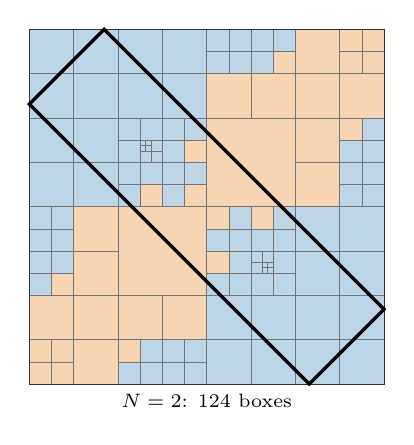
\begin{tikzpicture}[scale=0.95]
\fill[regB!30] (4.4458,0.7036) rectangle (4.7422,1);
\fill[regB!30] (4.1494,0.7036) rectangle (4.4458,1);
\fill[regB!30] (4.4458,0.4072) rectangle (4.7422,0.7036);
\fill[regB!30] (4.1494,0.4072) rectangle (4.4458,0.7036);
\fill[regB!30] (3.5566,0.4072) rectangle (4.1494,1);
\fill[regB!30] (4.1494,-0.1855) rectangle (4.7422,0.4072);
\fill[regB!30] (3.5566,-0.1855) rectangle (4.1494,0.4072);
\fill[regA!30] (3.2603,0.7036) rectangle (3.5566,1);
\fill[regA!30] (2.9639,0.7036) rectangle (3.2603,1);
\fill[regB!30] (3.2603,0.4072) rectangle (3.5566,0.7036);
\fill[regA!30] (2.9639,0.4072) rectangle (3.2603,0.7036);
\fill[regA!30] (2.6675,0.7036) rectangle (2.9639,1);
\fill[regA!30] (2.3711,0.7036) rectangle (2.6675,1);
\fill[regA!30] (2.6675,0.4072) rectangle (2.9639,0.7036);
\fill[regA!30] (2.3711,0.4072) rectangle (2.6675,0.7036);
\fill[regB!30] (2.9639,-0.1855) rectangle (3.5566,0.4072);
\fill[regB!30] (2.3711,-0.1855) rectangle (2.9639,0.4072);
\fill[regA!30] (4.4458,-0.4819) rectangle (4.7422,-0.1855);
\fill[regB!30] (4.1494,-0.4819) rectangle (4.4458,-0.1855);
\fill[regA!30] (4.4458,-0.7783) rectangle (4.7422,-0.4819);
\fill[regA!30] (4.1494,-0.7783) rectangle (4.4458,-0.4819);
\fill[regB!30] (3.5566,-0.7783) rectangle (4.1494,-0.1855);
\fill[regA!30] (4.4458,-1.0747) rectangle (4.7422,-0.7783);
\fill[regA!30] (4.1494,-1.0747) rectangle (4.4458,-0.7783);
\fill[regA!30] (4.4458,-1.3711) rectangle (4.7422,-1.0747);
\fill[regA!30] (4.1494,-1.3711) rectangle (4.4458,-1.0747);
\fill[regB!30] (3.5566,-1.3711) rectangle (4.1494,-0.7783);
\fill[regB!30] (2.3711,-1.3711) rectangle (3.5566,-0.1855);
\fill[regA!30] (1.7783,0.4072) rectangle (2.3711,1);
\fill[regA!30] (1.1855,0.4072) rectangle (1.7783,1);
\fill[regA!30] (1.7783,-0.1855) rectangle (2.3711,0.4072);
\fill[regA!30] (1.1855,-0.1855) rectangle (1.7783,0.4072);
\fill[regA!30] (0.5928,0.4072) rectangle (1.1855,1);
\fill[regA!30] (0,0.4072) rectangle (0.5928,1);
\fill[regA!30] (0.5928,-0.1855) rectangle (1.1855,0.4072);
\fill[regA!30] (0,-0.1855) rectangle (0.5928,0.4072);
\fill[regA!30] (2.0747,-0.4819) rectangle (2.3711,-0.1855);
\fill[regA!30] (1.7783,-0.4819) rectangle (2.0747,-0.1855);
\fill[regB!30] (2.0747,-0.7783) rectangle (2.3711,-0.4819);
\fill[regA!30] (1.7783,-0.7783) rectangle (2.0747,-0.4819);
\fill[regA!30] (1.4819,-0.4819) rectangle (1.7783,-0.1855);
\fill[regA!30] (1.1855,-0.4819) rectangle (1.4819,-0.1855);
\fill[regA!30] (1.6301,-0.6301) rectangle (1.7783,-0.4819);
\fill[regA!30] (1.556,-0.556) rectangle (1.6301,-0.4819);
\fill[regA!30] (1.4819,-0.556) rectangle (1.556,-0.4819);
\fill[regA!30] (1.556,-0.6301) rectangle (1.6301,-0.556);
\fill[regA!30] (1.4819,-0.6301) rectangle (1.556,-0.556);
\fill[regA!30] (1.6301,-0.7783) rectangle (1.7783,-0.6301);
\fill[regA!30] (1.4819,-0.7783) rectangle (1.6301,-0.6301);
\fill[regA!30] (1.1855,-0.7783) rectangle (1.4819,-0.4819);
\fill[regA!30] (2.0747,-1.0747) rectangle (2.3711,-0.7783);
\fill[regA!30] (1.7783,-1.0747) rectangle (2.0747,-0.7783);
\fill[regB!30] (2.0747,-1.3711) rectangle (2.3711,-1.0747);
\fill[regA!30] (1.7783,-1.3711) rectangle (2.0747,-1.0747);
\fill[regA!30] (1.4819,-1.0747) rectangle (1.7783,-0.7783);
\fill[regA!30] (1.1855,-1.0747) rectangle (1.4819,-0.7783);
\fill[regB!30] (1.4819,-1.3711) rectangle (1.7783,-1.0747);
\fill[regA!30] (1.1855,-1.3711) rectangle (1.4819,-1.0747);
\fill[regA!30] (0.5928,-0.7783) rectangle (1.1855,-0.1855);
\fill[regA!30] (0,-0.7783) rectangle (0.5928,-0.1855);
\fill[regA!30] (0.5928,-1.3711) rectangle (1.1855,-0.7783);
\fill[regA!30] (0,-1.3711) rectangle (0.5928,-0.7783);
\fill[regA!30] (4.1494,-1.9639) rectangle (4.7422,-1.3711);
\fill[regA!30] (3.5566,-1.9639) rectangle (4.1494,-1.3711);
\fill[regA!30] (4.1494,-2.5566) rectangle (4.7422,-1.9639);
\fill[regA!30] (3.5566,-2.5566) rectangle (4.1494,-1.9639);
\fill[regA!30] (3.2603,-1.6675) rectangle (3.5566,-1.3711);
\fill[regB!30] (2.9639,-1.6675) rectangle (3.2603,-1.3711);
\fill[regA!30] (3.2603,-1.9639) rectangle (3.5566,-1.6675);
\fill[regA!30] (2.9639,-1.9639) rectangle (3.2603,-1.6675);
\fill[regA!30] (2.6675,-1.6675) rectangle (2.9639,-1.3711);
\fill[regB!30] (2.3711,-1.6675) rectangle (2.6675,-1.3711);
\fill[regA!30] (2.6675,-1.9639) rectangle (2.9639,-1.6675);
\fill[regA!30] (2.3711,-1.9639) rectangle (2.6675,-1.6675);
\fill[regA!30] (3.2603,-2.2603) rectangle (3.5566,-1.9639);
\fill[regA!30] (3.1121,-2.1121) rectangle (3.2603,-1.9639);
\fill[regA!30] (2.9639,-2.1121) rectangle (3.1121,-1.9639);
\fill[regA!30] (3.1862,-2.1862) rectangle (3.2603,-2.1121);
\fill[regA!30] (3.1121,-2.1862) rectangle (3.1862,-2.1121);
\fill[regA!30] (3.1862,-2.2603) rectangle (3.2603,-2.1862);
\fill[regA!30] (3.1121,-2.2603) rectangle (3.1862,-2.1862);
\fill[regA!30] (2.9639,-2.2603) rectangle (3.1121,-2.1121);
\fill[regA!30] (3.2603,-2.5566) rectangle (3.5566,-2.2603);
\fill[regA!30] (2.9639,-2.5566) rectangle (3.2603,-2.2603);
\fill[regA!30] (2.6675,-2.2603) rectangle (2.9639,-1.9639);
\fill[regB!30] (2.3711,-2.2603) rectangle (2.6675,-1.9639);
\fill[regA!30] (2.6675,-2.5566) rectangle (2.9639,-2.2603);
\fill[regA!30] (2.3711,-2.5566) rectangle (2.6675,-2.2603);
\fill[regA!30] (4.1494,-3.1494) rectangle (4.7422,-2.5566);
\fill[regA!30] (3.5566,-3.1494) rectangle (4.1494,-2.5566);
\fill[regA!30] (4.1494,-3.7422) rectangle (4.7422,-3.1494);
\fill[regA!30] (3.5566,-3.7422) rectangle (4.1494,-3.1494);
\fill[regA!30] (2.9639,-3.1494) rectangle (3.5566,-2.5566);
\fill[regA!30] (2.3711,-3.1494) rectangle (2.9639,-2.5566);
\fill[regA!30] (2.9639,-3.7422) rectangle (3.5566,-3.1494);
\fill[regA!30] (2.3711,-3.7422) rectangle (2.9639,-3.1494);
\fill[regB!30] (1.1855,-2.5566) rectangle (2.3711,-1.3711);
\fill[regB!30] (0.5928,-1.9639) rectangle (1.1855,-1.3711);
\fill[regA!30] (0.2964,-1.6675) rectangle (0.5928,-1.3711);
\fill[regA!30] (0,-1.6675) rectangle (0.2964,-1.3711);
\fill[regA!30] (0.2964,-1.9639) rectangle (0.5928,-1.6675);
\fill[regA!30] (0,-1.9639) rectangle (0.2964,-1.6675);
\fill[regB!30] (0.5928,-2.5566) rectangle (1.1855,-1.9639);
\fill[regA!30] (0.2964,-2.2603) rectangle (0.5928,-1.9639);
\fill[regA!30] (0,-2.2603) rectangle (0.2964,-1.9639);
\fill[regB!30] (0.2964,-2.5566) rectangle (0.5928,-2.2603);
\fill[regA!30] (0,-2.5566) rectangle (0.2964,-2.2603);
\fill[regB!30] (1.7783,-3.1494) rectangle (2.3711,-2.5566);
\fill[regB!30] (1.1855,-3.1494) rectangle (1.7783,-2.5566);
\fill[regA!30] (2.0747,-3.4458) rectangle (2.3711,-3.1494);
\fill[regA!30] (1.7783,-3.4458) rectangle (2.0747,-3.1494);
\fill[regA!30] (2.0747,-3.7422) rectangle (2.3711,-3.4458);
\fill[regA!30] (1.7783,-3.7422) rectangle (2.0747,-3.4458);
\fill[regA!30] (1.4819,-3.4458) rectangle (1.7783,-3.1494);
\fill[regB!30] (1.1855,-3.4458) rectangle (1.4819,-3.1494);
\fill[regA!30] (1.4819,-3.7422) rectangle (1.7783,-3.4458);
\fill[regA!30] (1.1855,-3.7422) rectangle (1.4819,-3.4458);
\fill[regB!30] (0.5928,-3.1494) rectangle (1.1855,-2.5566);
\fill[regB!30] (0,-3.1494) rectangle (0.5928,-2.5566);
\fill[regB!30] (0.5928,-3.7422) rectangle (1.1855,-3.1494);
\fill[regB!30] (0.2964,-3.4458) rectangle (0.5928,-3.1494);
\fill[regB!30] (0,-3.4458) rectangle (0.2964,-3.1494);
\fill[regB!30] (0.2964,-3.7422) rectangle (0.5928,-3.4458);
\fill[regB!30] (0,-3.7422) rectangle (0.2964,-3.4458);
\draw[black!55, line width=0.2pt] (4.4458,0.7036) rectangle (4.7422,1);
\draw[black!55, line width=0.2pt] (4.1494,0.7036) rectangle (4.4458,1);
\draw[black!55, line width=0.2pt] (4.4458,0.4072) rectangle (4.7422,0.7036);
\draw[black!55, line width=0.2pt] (4.1494,0.4072) rectangle (4.4458,0.7036);
\draw[black!55, line width=0.2pt] (3.5566,0.4072) rectangle (4.1494,1);
\draw[black!55, line width=0.2pt] (4.1494,-0.1855) rectangle (4.7422,0.4072);
\draw[black!55, line width=0.2pt] (3.5566,-0.1855) rectangle (4.1494,0.4072);
\draw[black!55, line width=0.2pt] (3.2603,0.7036) rectangle (3.5566,1);
\draw[black!55, line width=0.2pt] (2.9639,0.7036) rectangle (3.2603,1);
\draw[black!55, line width=0.2pt] (3.2603,0.4072) rectangle (3.5566,0.7036);
\draw[black!55, line width=0.2pt] (2.9639,0.4072) rectangle (3.2603,0.7036);
\draw[black!55, line width=0.2pt] (2.6675,0.7036) rectangle (2.9639,1);
\draw[black!55, line width=0.2pt] (2.3711,0.7036) rectangle (2.6675,1);
\draw[black!55, line width=0.2pt] (2.6675,0.4072) rectangle (2.9639,0.7036);
\draw[black!55, line width=0.2pt] (2.3711,0.4072) rectangle (2.6675,0.7036);
\draw[black!55, line width=0.2pt] (2.9639,-0.1855) rectangle (3.5566,0.4072);
\draw[black!55, line width=0.2pt] (2.3711,-0.1855) rectangle (2.9639,0.4072);
\draw[black!55, line width=0.2pt] (4.4458,-0.4819) rectangle (4.7422,-0.1855);
\draw[black!55, line width=0.2pt] (4.1494,-0.4819) rectangle (4.4458,-0.1855);
\draw[black!55, line width=0.2pt] (4.4458,-0.7783) rectangle (4.7422,-0.4819);
\draw[black!55, line width=0.2pt] (4.1494,-0.7783) rectangle (4.4458,-0.4819);
\draw[black!55, line width=0.2pt] (3.5566,-0.7783) rectangle (4.1494,-0.1855);
\draw[black!55, line width=0.2pt] (4.4458,-1.0747) rectangle (4.7422,-0.7783);
\draw[black!55, line width=0.2pt] (4.1494,-1.0747) rectangle (4.4458,-0.7783);
\draw[black!55, line width=0.2pt] (4.4458,-1.3711) rectangle (4.7422,-1.0747);
\draw[black!55, line width=0.2pt] (4.1494,-1.3711) rectangle (4.4458,-1.0747);
\draw[black!55, line width=0.2pt] (3.5566,-1.3711) rectangle (4.1494,-0.7783);
\draw[black!55, line width=0.2pt] (2.3711,-1.3711) rectangle (3.5566,-0.1855);
\draw[black!55, line width=0.2pt] (1.7783,0.4072) rectangle (2.3711,1);
\draw[black!55, line width=0.2pt] (1.1855,0.4072) rectangle (1.7783,1);
\draw[black!55, line width=0.2pt] (1.7783,-0.1855) rectangle (2.3711,0.4072);
\draw[black!55, line width=0.2pt] (1.1855,-0.1855) rectangle (1.7783,0.4072);
\draw[black!55, line width=0.2pt] (0.5928,0.4072) rectangle (1.1855,1);
\draw[black!55, line width=0.2pt] (0,0.4072) rectangle (0.5928,1);
\draw[black!55, line width=0.2pt] (0.5928,-0.1855) rectangle (1.1855,0.4072);
\draw[black!55, line width=0.2pt] (0,-0.1855) rectangle (0.5928,0.4072);
\draw[black!55, line width=0.2pt] (2.0747,-0.4819) rectangle (2.3711,-0.1855);
\draw[black!55, line width=0.2pt] (1.7783,-0.4819) rectangle (2.0747,-0.1855);
\draw[black!55, line width=0.2pt] (2.0747,-0.7783) rectangle (2.3711,-0.4819);
\draw[black!55, line width=0.2pt] (1.7783,-0.7783) rectangle (2.0747,-0.4819);
\draw[black!55, line width=0.2pt] (1.4819,-0.4819) rectangle (1.7783,-0.1855);
\draw[black!55, line width=0.2pt] (1.1855,-0.4819) rectangle (1.4819,-0.1855);
\draw[black!55, line width=0.2pt] (1.6301,-0.6301) rectangle (1.7783,-0.4819);
\draw[black!55, line width=0.2pt] (1.556,-0.556) rectangle (1.6301,-0.4819);
\draw[black!55, line width=0.2pt] (1.4819,-0.556) rectangle (1.556,-0.4819);
\draw[black!55, line width=0.2pt] (1.556,-0.6301) rectangle (1.6301,-0.556);
\draw[black!55, line width=0.2pt] (1.4819,-0.6301) rectangle (1.556,-0.556);
\draw[black!55, line width=0.2pt] (1.6301,-0.7783) rectangle (1.7783,-0.6301);
\draw[black!55, line width=0.2pt] (1.4819,-0.7783) rectangle (1.6301,-0.6301);
\draw[black!55, line width=0.2pt] (1.1855,-0.7783) rectangle (1.4819,-0.4819);
\draw[black!55, line width=0.2pt] (2.0747,-1.0747) rectangle (2.3711,-0.7783);
\draw[black!55, line width=0.2pt] (1.7783,-1.0747) rectangle (2.0747,-0.7783);
\draw[black!55, line width=0.2pt] (2.0747,-1.3711) rectangle (2.3711,-1.0747);
\draw[black!55, line width=0.2pt] (1.7783,-1.3711) rectangle (2.0747,-1.0747);
\draw[black!55, line width=0.2pt] (1.4819,-1.0747) rectangle (1.7783,-0.7783);
\draw[black!55, line width=0.2pt] (1.1855,-1.0747) rectangle (1.4819,-0.7783);
\draw[black!55, line width=0.2pt] (1.4819,-1.3711) rectangle (1.7783,-1.0747);
\draw[black!55, line width=0.2pt] (1.1855,-1.3711) rectangle (1.4819,-1.0747);
\draw[black!55, line width=0.2pt] (0.5928,-0.7783) rectangle (1.1855,-0.1855);
\draw[black!55, line width=0.2pt] (0,-0.7783) rectangle (0.5928,-0.1855);
\draw[black!55, line width=0.2pt] (0.5928,-1.3711) rectangle (1.1855,-0.7783);
\draw[black!55, line width=0.2pt] (0,-1.3711) rectangle (0.5928,-0.7783);
\draw[black!55, line width=0.2pt] (4.1494,-1.9639) rectangle (4.7422,-1.3711);
\draw[black!55, line width=0.2pt] (3.5566,-1.9639) rectangle (4.1494,-1.3711);
\draw[black!55, line width=0.2pt] (4.1494,-2.5566) rectangle (4.7422,-1.9639);
\draw[black!55, line width=0.2pt] (3.5566,-2.5566) rectangle (4.1494,-1.9639);
\draw[black!55, line width=0.2pt] (3.2603,-1.6675) rectangle (3.5566,-1.3711);
\draw[black!55, line width=0.2pt] (2.9639,-1.6675) rectangle (3.2603,-1.3711);
\draw[black!55, line width=0.2pt] (3.2603,-1.9639) rectangle (3.5566,-1.6675);
\draw[black!55, line width=0.2pt] (2.9639,-1.9639) rectangle (3.2603,-1.6675);
\draw[black!55, line width=0.2pt] (2.6675,-1.6675) rectangle (2.9639,-1.3711);
\draw[black!55, line width=0.2pt] (2.3711,-1.6675) rectangle (2.6675,-1.3711);
\draw[black!55, line width=0.2pt] (2.6675,-1.9639) rectangle (2.9639,-1.6675);
\draw[black!55, line width=0.2pt] (2.3711,-1.9639) rectangle (2.6675,-1.6675);
\draw[black!55, line width=0.2pt] (3.2603,-2.2603) rectangle (3.5566,-1.9639);
\draw[black!55, line width=0.2pt] (3.1121,-2.1121) rectangle (3.2603,-1.9639);
\draw[black!55, line width=0.2pt] (2.9639,-2.1121) rectangle (3.1121,-1.9639);
\draw[black!55, line width=0.2pt] (3.1862,-2.1862) rectangle (3.2603,-2.1121);
\draw[black!55, line width=0.2pt] (3.1121,-2.1862) rectangle (3.1862,-2.1121);
\draw[black!55, line width=0.2pt] (3.1862,-2.2603) rectangle (3.2603,-2.1862);
\draw[black!55, line width=0.2pt] (3.1121,-2.2603) rectangle (3.1862,-2.1862);
\draw[black!55, line width=0.2pt] (2.9639,-2.2603) rectangle (3.1121,-2.1121);
\draw[black!55, line width=0.2pt] (3.2603,-2.5566) rectangle (3.5566,-2.2603);
\draw[black!55, line width=0.2pt] (2.9639,-2.5566) rectangle (3.2603,-2.2603);
\draw[black!55, line width=0.2pt] (2.6675,-2.2603) rectangle (2.9639,-1.9639);
\draw[black!55, line width=0.2pt] (2.3711,-2.2603) rectangle (2.6675,-1.9639);
\draw[black!55, line width=0.2pt] (2.6675,-2.5566) rectangle (2.9639,-2.2603);
\draw[black!55, line width=0.2pt] (2.3711,-2.5566) rectangle (2.6675,-2.2603);
\draw[black!55, line width=0.2pt] (4.1494,-3.1494) rectangle (4.7422,-2.5566);
\draw[black!55, line width=0.2pt] (3.5566,-3.1494) rectangle (4.1494,-2.5566);
\draw[black!55, line width=0.2pt] (4.1494,-3.7422) rectangle (4.7422,-3.1494);
\draw[black!55, line width=0.2pt] (3.5566,-3.7422) rectangle (4.1494,-3.1494);
\draw[black!55, line width=0.2pt] (2.9639,-3.1494) rectangle (3.5566,-2.5566);
\draw[black!55, line width=0.2pt] (2.3711,-3.1494) rectangle (2.9639,-2.5566);
\draw[black!55, line width=0.2pt] (2.9639,-3.7422) rectangle (3.5566,-3.1494);
\draw[black!55, line width=0.2pt] (2.3711,-3.7422) rectangle (2.9639,-3.1494);
\draw[black!55, line width=0.2pt] (1.1855,-2.5566) rectangle (2.3711,-1.3711);
\draw[black!55, line width=0.2pt] (0.5928,-1.9639) rectangle (1.1855,-1.3711);
\draw[black!55, line width=0.2pt] (0.2964,-1.6675) rectangle (0.5928,-1.3711);
\draw[black!55, line width=0.2pt] (0,-1.6675) rectangle (0.2964,-1.3711);
\draw[black!55, line width=0.2pt] (0.2964,-1.9639) rectangle (0.5928,-1.6675);
\draw[black!55, line width=0.2pt] (0,-1.9639) rectangle (0.2964,-1.6675);
\draw[black!55, line width=0.2pt] (0.5928,-2.5566) rectangle (1.1855,-1.9639);
\draw[black!55, line width=0.2pt] (0.2964,-2.2603) rectangle (0.5928,-1.9639);
\draw[black!55, line width=0.2pt] (0,-2.2603) rectangle (0.2964,-1.9639);
\draw[black!55, line width=0.2pt] (0.2964,-2.5566) rectangle (0.5928,-2.2603);
\draw[black!55, line width=0.2pt] (0,-2.5566) rectangle (0.2964,-2.2603);
\draw[black!55, line width=0.2pt] (1.7783,-3.1494) rectangle (2.3711,-2.5566);
\draw[black!55, line width=0.2pt] (1.1855,-3.1494) rectangle (1.7783,-2.5566);
\draw[black!55, line width=0.2pt] (2.0747,-3.4458) rectangle (2.3711,-3.1494);
\draw[black!55, line width=0.2pt] (1.7783,-3.4458) rectangle (2.0747,-3.1494);
\draw[black!55, line width=0.2pt] (2.0747,-3.7422) rectangle (2.3711,-3.4458);
\draw[black!55, line width=0.2pt] (1.7783,-3.7422) rectangle (2.0747,-3.4458);
\draw[black!55, line width=0.2pt] (1.4819,-3.4458) rectangle (1.7783,-3.1494);
\draw[black!55, line width=0.2pt] (1.1855,-3.4458) rectangle (1.4819,-3.1494);
\draw[black!55, line width=0.2pt] (1.4819,-3.7422) rectangle (1.7783,-3.4458);
\draw[black!55, line width=0.2pt] (1.1855,-3.7422) rectangle (1.4819,-3.4458);
\draw[black!55, line width=0.2pt] (0.5928,-3.1494) rectangle (1.1855,-2.5566);
\draw[black!55, line width=0.2pt] (0,-3.1494) rectangle (0.5928,-2.5566);
\draw[black!55, line width=0.2pt] (0.5928,-3.7422) rectangle (1.1855,-3.1494);
\draw[black!55, line width=0.2pt] (0.2964,-3.4458) rectangle (0.5928,-3.1494);
\draw[black!55, line width=0.2pt] (0,-3.4458) rectangle (0.2964,-3.1494);
\draw[black!55, line width=0.2pt] (0.2964,-3.7422) rectangle (0.5928,-3.4458);
\draw[black!55, line width=0.2pt] (0,-3.7422) rectangle (0.2964,-3.4458);
\draw[black!80, thin] (0,-3.7422) rectangle (4.7422,1);
\draw[very thick] (0,0) -- (1,1) -- (4.7417,-2.7417) -- (3.7417,-3.7417) -- cycle;
\node[font=\scriptsize, below] at (2.3711,-3.7422) {$N=2$: 124 boxes};
\end{tikzpicture}

\caption{\textbf{SOLVE} on $R_0\supset D$ for $\Q(\sqrt{14})$, $T=3$. Left: $N=1$; red boxes
(depth $6$) cannot be certified with unit denominators. Right: $N=2$; boxes shaded by the norm of
the denominator of a region containing them, $1$ (blue) or $2$ (orange). The thick parallelogram
is $D$.}
\label{fig:q-solve}
\end{figure}

\begin{figure}[ht]
\centering
% generated by gen_figures.py (F = Q(sqrt 14)); do not edit by hand
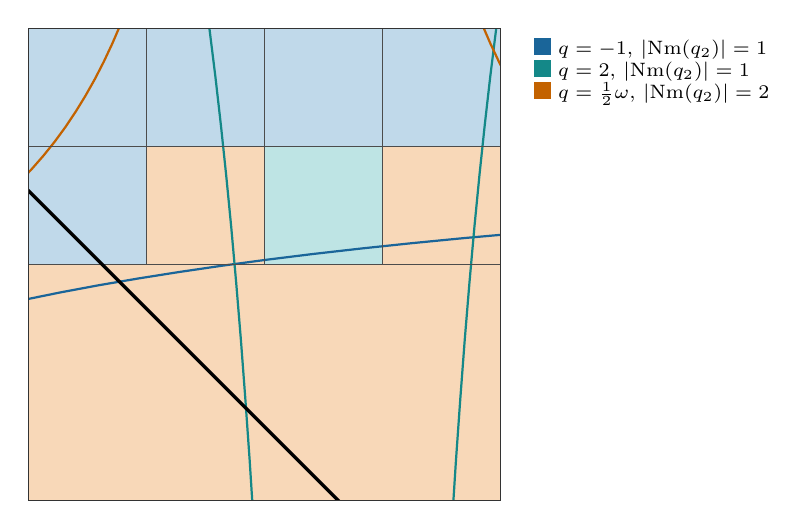
\begin{tikzpicture}[scale=5.061]
\begin{scope}\clip (1.1855,-1.9639) rectangle (2.3711,-0.7783);
\fill[zA!28] (2.0747,-1.0747) rectangle (2.3711,-0.7783);
\fill[zA!28] (1.7783,-1.0747) rectangle (2.0747,-0.7783);
\fill[zD!28] (2.0747,-1.3711) rectangle (2.3711,-1.0747);
\fill[zB!28] (1.7783,-1.3711) rectangle (2.0747,-1.0747);
\fill[zA!28] (1.4819,-1.0747) rectangle (1.7783,-0.7783);
\fill[zA!28] (1.1855,-1.0747) rectangle (1.4819,-0.7783);
\fill[zD!28] (1.4819,-1.3711) rectangle (1.7783,-1.0747);
\fill[zA!28] (1.1855,-1.3711) rectangle (1.4819,-1.0747);
\fill[zD!28] (1.1855,-2.5566) rectangle (2.3711,-1.3711);
\draw[zA!85!black, thick] (-0.9833,59) -- (-0.9826,56.593) -- (-0.9819,54.2826) -- (-0.9812,52.0648) -- (-0.9804,49.936) -- (-0.9795,47.8927) -- (-0.9787,45.9313) -- (-0.9778,44.0485) -- (-0.9769,42.2413) -- (-0.9759,40.5066) -- (-0.9749,38.8415) -- (-0.9739,37.2432) -- (-0.9728,35.709) -- (-0.9716,34.2364) -- (-0.9704,32.8228) -- (-0.9692,31.466) -- (-0.9679,30.1636) -- (-0.9666,28.9134) -- (-0.9652,27.7134) -- (-0.9637,26.5615) -- (-0.9622,25.4558) -- (-0.9606,24.3945) -- (-0.959,23.3757) -- (-0.9573,22.3979) -- (-0.9555,21.4592) -- (-0.9536,20.5582) -- (-0.9517,19.6934) -- (-0.9497,18.8633) -- (-0.9476,18.0664) -- (-0.9454,17.3015) -- (-0.9431,16.5673) -- (-0.9407,15.8626) -- (-0.9382,15.1861) -- (-0.9356,14.5368) -- (-0.9329,13.9135) -- (-0.9301,13.3152) -- (-0.9272,12.741) -- (-0.9242,12.1897) -- (-0.921,11.6606) -- (-0.9177,11.1527) -- (-0.9143,10.6652) -- (-0.9107,10.1972) -- (-0.907,9.748) -- (-0.9031,9.3168) -- (-0.899,8.903) -- (-0.8948,8.5057) -- (-0.8904,8.1243) -- (-0.8858,7.7583) -- (-0.8811,7.407) -- (-0.8761,7.0697) -- (-0.8709,6.746) -- (-0.8655,6.4352) -- (-0.8599,6.1369) -- (-0.854,5.8506) -- (-0.8479,5.5758) -- (-0.8416,5.312) -- (-0.835,5.0588) -- (-0.8281,4.8157) -- (-0.8209,4.5824) -- (-0.8134,4.3585) -- (-0.8056,4.1435) -- (-0.7975,3.9372) -- (-0.789,3.7391) -- (-0.7802,3.549) -- (-0.771,3.3665) -- (-0.7614,3.1913) -- (-0.7514,3.0232) -- (-0.7411,2.8618) -- (-0.7302,2.7069) -- (-0.719,2.5582) -- (-0.7072,2.4154) -- (-0.695,2.2784) -- (-0.6822,2.1469) -- (-0.6689,2.0207) -- (-0.6551,1.8995) -- (-0.6407,1.7832) -- (-0.6257,1.6715) -- (-0.61,1.5643) -- (-0.5937,1.4615) -- (-0.5768,1.3627) -- (-0.5591,1.2679) -- (-0.5406,1.177) -- (-0.5214,1.0896) -- (-0.5014,1.0058) -- (-0.4806,0.9253) -- (-0.4589,0.8481) -- (-0.4363,0.7739) -- (-0.4127,0.7028) -- (-0.3882,0.6345) -- (-0.3626,0.5689) -- (-0.336,0.506) -- (-0.3082,0.4456) -- (-0.2793,0.3876) -- (-0.2492,0.3319) -- (-0.2178,0.2785) -- (-0.1851,0.2272) -- (-0.1511,0.1779) -- (-0.1156,0.1307) -- (-0.0786,0.0853) -- (-0.0401,0.0418) -- (0,0) -- (0.0418,-0.0401) -- (0.0853,-0.0786) -- (0.1307,-0.1156) -- (0.1779,-0.1511) -- (0.2272,-0.1851) -- (0.2785,-0.2178) -- (0.3319,-0.2492) -- (0.3876,-0.2793) -- (0.4456,-0.3082) -- (0.506,-0.336) -- (0.5689,-0.3626) -- (0.6345,-0.3882) -- (0.7028,-0.4127) -- (0.7739,-0.4363) -- (0.8481,-0.4589) -- (0.9253,-0.4806) -- (1.0058,-0.5014) -- (1.0896,-0.5214) -- (1.177,-0.5406) -- (1.2679,-0.5591) -- (1.3627,-0.5768) -- (1.4615,-0.5937) -- (1.5643,-0.61) -- (1.6715,-0.6257) -- (1.7832,-0.6407) -- (1.8995,-0.6551) -- (2.0207,-0.6689) -- (2.1469,-0.6822) -- (2.2784,-0.695) -- (2.4154,-0.7072) -- (2.5582,-0.719) -- (2.7069,-0.7302) -- (2.8618,-0.7411) -- (3.0232,-0.7514) -- (3.1913,-0.7614) -- (3.3665,-0.771) -- (3.549,-0.7802) -- (3.7391,-0.789) -- (3.9372,-0.7975) -- (4.1435,-0.8056) -- (4.3585,-0.8134) -- (4.5824,-0.8209) -- (4.8157,-0.8281) -- (5.0588,-0.835) -- (5.312,-0.8416) -- (5.5758,-0.8479) -- (5.8506,-0.854) -- (6.1369,-0.8599) -- (6.4352,-0.8655) -- (6.746,-0.8709) -- (7.0697,-0.8761) -- (7.407,-0.8811) -- (7.7583,-0.8858) -- (8.1243,-0.8904) -- (8.5057,-0.8948) -- (8.903,-0.899) -- (9.3168,-0.9031) -- (9.748,-0.907) -- (10.1972,-0.9107) -- (10.6652,-0.9143) -- (11.1527,-0.9177) -- (11.6606,-0.921) -- (12.1897,-0.9242) -- (12.741,-0.9272) -- (13.3152,-0.9301) -- (13.9135,-0.9329) -- (14.5368,-0.9356) -- (15.1861,-0.9382) -- (15.8626,-0.9407) -- (16.5673,-0.9431) -- (17.3015,-0.9454) -- (18.0664,-0.9476) -- (18.8633,-0.9497) -- (19.6934,-0.9517) -- (20.5582,-0.9536) -- (21.4592,-0.9555) -- (22.3979,-0.9573) -- (23.3757,-0.959) -- (24.3945,-0.9606) -- (25.4558,-0.9622) -- (26.5615,-0.9637) -- (27.7134,-0.9652) -- (28.9134,-0.9666) -- (30.1636,-0.9679) -- (31.466,-0.9692) -- (32.8228,-0.9704) -- (34.2364,-0.9716) -- (35.709,-0.9728) -- (37.2432,-0.9739) -- (38.8415,-0.9749) -- (40.5066,-0.9759) -- (42.2413,-0.9769) -- (44.0485,-0.9778) -- (45.9313,-0.9787) -- (47.8927,-0.9795) -- (49.936,-0.9804) -- (52.0648,-0.9812) -- (54.2826,-0.9819) -- (56.593,-0.9826) -- (59,-0.9833);
\draw[zA!85!black, thick] (-1.0167,59) -- (-1.0174,56.593) -- (-1.0181,54.2826) -- (-1.0188,52.0648) -- (-1.0196,49.936) -- (-1.0205,47.8927) -- (-1.0213,45.9313) -- (-1.0222,44.0485) -- (-1.0231,42.2413) -- (-1.0241,40.5066) -- (-1.0251,38.8415) -- (-1.0261,37.2432) -- (-1.0272,35.709) -- (-1.0284,34.2364) -- (-1.0296,32.8228) -- (-1.0308,31.466) -- (-1.0321,30.1636) -- (-1.0334,28.9134) -- (-1.0348,27.7134) -- (-1.0363,26.5615) -- (-1.0378,25.4558) -- (-1.0394,24.3945) -- (-1.041,23.3757) -- (-1.0427,22.3979) -- (-1.0445,21.4592) -- (-1.0464,20.5582) -- (-1.0483,19.6934) -- (-1.0503,18.8633) -- (-1.0524,18.0664) -- (-1.0546,17.3015) -- (-1.0569,16.5673) -- (-1.0593,15.8626) -- (-1.0618,15.1861) -- (-1.0644,14.5368) -- (-1.0671,13.9135) -- (-1.0699,13.3152) -- (-1.0728,12.741) -- (-1.0758,12.1897) -- (-1.079,11.6606) -- (-1.0823,11.1527) -- (-1.0857,10.6652) -- (-1.0893,10.1972) -- (-1.093,9.748) -- (-1.0969,9.3168) -- (-1.101,8.903) -- (-1.1052,8.5057) -- (-1.1096,8.1243) -- (-1.1142,7.7583) -- (-1.1189,7.407) -- (-1.1239,7.0697) -- (-1.1291,6.746) -- (-1.1345,6.4352) -- (-1.1401,6.1369) -- (-1.146,5.8506) -- (-1.1521,5.5758) -- (-1.1584,5.312) -- (-1.165,5.0588) -- (-1.1719,4.8157) -- (-1.1791,4.5824) -- (-1.1866,4.3585) -- (-1.1944,4.1435) -- (-1.2025,3.9372) -- (-1.211,3.7391) -- (-1.2198,3.549) -- (-1.229,3.3665) -- (-1.2386,3.1913) -- (-1.2486,3.0232) -- (-1.2589,2.8618) -- (-1.2698,2.7069) -- (-1.281,2.5582) -- (-1.2928,2.4154) -- (-1.305,2.2784) -- (-1.3178,2.1469) -- (-1.3311,2.0207) -- (-1.3449,1.8995) -- (-1.3593,1.7832) -- (-1.3743,1.6715) -- (-1.39,1.5643) -- (-1.4063,1.4615) -- (-1.4232,1.3627) -- (-1.4409,1.2679) -- (-1.4594,1.177) -- (-1.4786,1.0896) -- (-1.4986,1.0058) -- (-1.5194,0.9253) -- (-1.5411,0.8481) -- (-1.5637,0.7739) -- (-1.5873,0.7028) -- (-1.6118,0.6345) -- (-1.6374,0.5689) -- (-1.664,0.506) -- (-1.6918,0.4456) -- (-1.7207,0.3876) -- (-1.7508,0.3319) -- (-1.7822,0.2785) -- (-1.8149,0.2272) -- (-1.8489,0.1779) -- (-1.8844,0.1307) -- (-1.9214,0.0853) -- (-1.9599,0.0418) -- (-2,0) -- (-2.0418,-0.0401) -- (-2.0853,-0.0786) -- (-2.1307,-0.1156) -- (-2.1779,-0.1511) -- (-2.2272,-0.1851) -- (-2.2785,-0.2178) -- (-2.3319,-0.2492) -- (-2.3876,-0.2793) -- (-2.4456,-0.3082) -- (-2.506,-0.336) -- (-2.5689,-0.3626) -- (-2.6345,-0.3882) -- (-2.7028,-0.4127) -- (-2.7739,-0.4363) -- (-2.8481,-0.4589) -- (-2.9253,-0.4806) -- (-3.0058,-0.5014) -- (-3.0896,-0.5214) -- (-3.177,-0.5406) -- (-3.2679,-0.5591) -- (-3.3627,-0.5768) -- (-3.4615,-0.5937) -- (-3.5643,-0.61) -- (-3.6715,-0.6257) -- (-3.7832,-0.6407) -- (-3.8995,-0.6551) -- (-4.0207,-0.6689) -- (-4.1469,-0.6822) -- (-4.2784,-0.695) -- (-4.4154,-0.7072) -- (-4.5582,-0.719) -- (-4.7069,-0.7302) -- (-4.8618,-0.7411) -- (-5.0232,-0.7514) -- (-5.1913,-0.7614) -- (-5.3665,-0.771) -- (-5.549,-0.7802) -- (-5.7391,-0.789) -- (-5.9372,-0.7975) -- (-6.1435,-0.8056) -- (-6.3585,-0.8134) -- (-6.5824,-0.8209) -- (-6.8157,-0.8281) -- (-7.0588,-0.835) -- (-7.312,-0.8416) -- (-7.5758,-0.8479) -- (-7.8506,-0.854) -- (-8.1369,-0.8599) -- (-8.4352,-0.8655) -- (-8.746,-0.8709) -- (-9.0697,-0.8761) -- (-9.407,-0.8811) -- (-9.7583,-0.8858) -- (-10.1243,-0.8904) -- (-10.5057,-0.8948) -- (-10.903,-0.899) -- (-11.3168,-0.9031) -- (-11.748,-0.907) -- (-12.1972,-0.9107) -- (-12.6652,-0.9143) -- (-13.1527,-0.9177) -- (-13.6606,-0.921) -- (-14.1897,-0.9242) -- (-14.741,-0.9272) -- (-15.3152,-0.9301) -- (-15.9135,-0.9329) -- (-16.5368,-0.9356) -- (-17.1861,-0.9382) -- (-17.8626,-0.9407) -- (-18.5673,-0.9431) -- (-19.3015,-0.9454) -- (-20.0664,-0.9476) -- (-20.8633,-0.9497) -- (-21.6934,-0.9517) -- (-22.5582,-0.9536) -- (-23.4592,-0.9555) -- (-24.3979,-0.9573) -- (-25.3757,-0.959) -- (-26.3945,-0.9606) -- (-27.4558,-0.9622) -- (-28.5615,-0.9637) -- (-29.7134,-0.9652) -- (-30.9134,-0.9666) -- (-32.1636,-0.9679) -- (-33.466,-0.9692) -- (-34.8228,-0.9704) -- (-36.2364,-0.9716) -- (-37.709,-0.9728) -- (-39.2432,-0.9739) -- (-40.8415,-0.9749) -- (-42.5066,-0.9759) -- (-44.2413,-0.9769) -- (-46.0485,-0.9778) -- (-47.9313,-0.9787) -- (-49.8927,-0.9795) -- (-51.936,-0.9804) -- (-54.0648,-0.9812) -- (-56.2826,-0.9819) -- (-58.593,-0.9826) -- (-61,-0.9833);
\draw[zA!85!black, thick] (-1.0167,-61) -- (-1.0174,-58.593) -- (-1.0181,-56.2826) -- (-1.0188,-54.0648) -- (-1.0196,-51.936) -- (-1.0205,-49.8927) -- (-1.0213,-47.9313) -- (-1.0222,-46.0485) -- (-1.0231,-44.2413) -- (-1.0241,-42.5066) -- (-1.0251,-40.8415) -- (-1.0261,-39.2432) -- (-1.0272,-37.709) -- (-1.0284,-36.2364) -- (-1.0296,-34.8228) -- (-1.0308,-33.466) -- (-1.0321,-32.1636) -- (-1.0334,-30.9134) -- (-1.0348,-29.7134) -- (-1.0363,-28.5615) -- (-1.0378,-27.4558) -- (-1.0394,-26.3945) -- (-1.041,-25.3757) -- (-1.0427,-24.3979) -- (-1.0445,-23.4592) -- (-1.0464,-22.5582) -- (-1.0483,-21.6934) -- (-1.0503,-20.8633) -- (-1.0524,-20.0664) -- (-1.0546,-19.3015) -- (-1.0569,-18.5673) -- (-1.0593,-17.8626) -- (-1.0618,-17.1861) -- (-1.0644,-16.5368) -- (-1.0671,-15.9135) -- (-1.0699,-15.3152) -- (-1.0728,-14.741) -- (-1.0758,-14.1897) -- (-1.079,-13.6606) -- (-1.0823,-13.1527) -- (-1.0857,-12.6652) -- (-1.0893,-12.1972) -- (-1.093,-11.748) -- (-1.0969,-11.3168) -- (-1.101,-10.903) -- (-1.1052,-10.5057) -- (-1.1096,-10.1243) -- (-1.1142,-9.7583) -- (-1.1189,-9.407) -- (-1.1239,-9.0697) -- (-1.1291,-8.746) -- (-1.1345,-8.4352) -- (-1.1401,-8.1369) -- (-1.146,-7.8506) -- (-1.1521,-7.5758) -- (-1.1584,-7.312) -- (-1.165,-7.0588) -- (-1.1719,-6.8157) -- (-1.1791,-6.5824) -- (-1.1866,-6.3585) -- (-1.1944,-6.1435) -- (-1.2025,-5.9372) -- (-1.211,-5.7391) -- (-1.2198,-5.549) -- (-1.229,-5.3665) -- (-1.2386,-5.1913) -- (-1.2486,-5.0232) -- (-1.2589,-4.8618) -- (-1.2698,-4.7069) -- (-1.281,-4.5582) -- (-1.2928,-4.4154) -- (-1.305,-4.2784) -- (-1.3178,-4.1469) -- (-1.3311,-4.0207) -- (-1.3449,-3.8995) -- (-1.3593,-3.7832) -- (-1.3743,-3.6715) -- (-1.39,-3.5643) -- (-1.4063,-3.4615) -- (-1.4232,-3.3627) -- (-1.4409,-3.2679) -- (-1.4594,-3.177) -- (-1.4786,-3.0896) -- (-1.4986,-3.0058) -- (-1.5194,-2.9253) -- (-1.5411,-2.8481) -- (-1.5637,-2.7739) -- (-1.5873,-2.7028) -- (-1.6118,-2.6345) -- (-1.6374,-2.5689) -- (-1.664,-2.506) -- (-1.6918,-2.4456) -- (-1.7207,-2.3876) -- (-1.7508,-2.3319) -- (-1.7822,-2.2785) -- (-1.8149,-2.2272) -- (-1.8489,-2.1779) -- (-1.8844,-2.1307) -- (-1.9214,-2.0853) -- (-1.9599,-2.0418) -- (-2,-2) -- (-2.0418,-1.9599) -- (-2.0853,-1.9214) -- (-2.1307,-1.8844) -- (-2.1779,-1.8489) -- (-2.2272,-1.8149) -- (-2.2785,-1.7822) -- (-2.3319,-1.7508) -- (-2.3876,-1.7207) -- (-2.4456,-1.6918) -- (-2.506,-1.664) -- (-2.5689,-1.6374) -- (-2.6345,-1.6118) -- (-2.7028,-1.5873) -- (-2.7739,-1.5637) -- (-2.8481,-1.5411) -- (-2.9253,-1.5194) -- (-3.0058,-1.4986) -- (-3.0896,-1.4786) -- (-3.177,-1.4594) -- (-3.2679,-1.4409) -- (-3.3627,-1.4232) -- (-3.4615,-1.4063) -- (-3.5643,-1.39) -- (-3.6715,-1.3743) -- (-3.7832,-1.3593) -- (-3.8995,-1.3449) -- (-4.0207,-1.3311) -- (-4.1469,-1.3178) -- (-4.2784,-1.305) -- (-4.4154,-1.2928) -- (-4.5582,-1.281) -- (-4.7069,-1.2698) -- (-4.8618,-1.2589) -- (-5.0232,-1.2486) -- (-5.1913,-1.2386) -- (-5.3665,-1.229) -- (-5.549,-1.2198) -- (-5.7391,-1.211) -- (-5.9372,-1.2025) -- (-6.1435,-1.1944) -- (-6.3585,-1.1866) -- (-6.5824,-1.1791) -- (-6.8157,-1.1719) -- (-7.0588,-1.165) -- (-7.312,-1.1584) -- (-7.5758,-1.1521) -- (-7.8506,-1.146) -- (-8.1369,-1.1401) -- (-8.4352,-1.1345) -- (-8.746,-1.1291) -- (-9.0697,-1.1239) -- (-9.407,-1.1189) -- (-9.7583,-1.1142) -- (-10.1243,-1.1096) -- (-10.5057,-1.1052) -- (-10.903,-1.101) -- (-11.3168,-1.0969) -- (-11.748,-1.093) -- (-12.1972,-1.0893) -- (-12.6652,-1.0857) -- (-13.1527,-1.0823) -- (-13.6606,-1.079) -- (-14.1897,-1.0758) -- (-14.741,-1.0728) -- (-15.3152,-1.0699) -- (-15.9135,-1.0671) -- (-16.5368,-1.0644) -- (-17.1861,-1.0618) -- (-17.8626,-1.0593) -- (-18.5673,-1.0569) -- (-19.3015,-1.0546) -- (-20.0664,-1.0524) -- (-20.8633,-1.0503) -- (-21.6934,-1.0483) -- (-22.5582,-1.0464) -- (-23.4592,-1.0445) -- (-24.3979,-1.0427) -- (-25.3757,-1.041) -- (-26.3945,-1.0394) -- (-27.4558,-1.0378) -- (-28.5615,-1.0363) -- (-29.7134,-1.0348) -- (-30.9134,-1.0334) -- (-32.1636,-1.0321) -- (-33.466,-1.0308) -- (-34.8228,-1.0296) -- (-36.2364,-1.0284) -- (-37.709,-1.0272) -- (-39.2432,-1.0261) -- (-40.8415,-1.0251) -- (-42.5066,-1.0241) -- (-44.2413,-1.0231) -- (-46.0485,-1.0222) -- (-47.9313,-1.0213) -- (-49.8927,-1.0205) -- (-51.936,-1.0196) -- (-54.0648,-1.0188) -- (-56.2826,-1.0181) -- (-58.593,-1.0174) -- (-61,-1.0167);
\draw[zA!85!black, thick] (-0.9833,-61) -- (-0.9826,-58.593) -- (-0.9819,-56.2826) -- (-0.9812,-54.0648) -- (-0.9804,-51.936) -- (-0.9795,-49.8927) -- (-0.9787,-47.9313) -- (-0.9778,-46.0485) -- (-0.9769,-44.2413) -- (-0.9759,-42.5066) -- (-0.9749,-40.8415) -- (-0.9739,-39.2432) -- (-0.9728,-37.709) -- (-0.9716,-36.2364) -- (-0.9704,-34.8228) -- (-0.9692,-33.466) -- (-0.9679,-32.1636) -- (-0.9666,-30.9134) -- (-0.9652,-29.7134) -- (-0.9637,-28.5615) -- (-0.9622,-27.4558) -- (-0.9606,-26.3945) -- (-0.959,-25.3757) -- (-0.9573,-24.3979) -- (-0.9555,-23.4592) -- (-0.9536,-22.5582) -- (-0.9517,-21.6934) -- (-0.9497,-20.8633) -- (-0.9476,-20.0664) -- (-0.9454,-19.3015) -- (-0.9431,-18.5673) -- (-0.9407,-17.8626) -- (-0.9382,-17.1861) -- (-0.9356,-16.5368) -- (-0.9329,-15.9135) -- (-0.9301,-15.3152) -- (-0.9272,-14.741) -- (-0.9242,-14.1897) -- (-0.921,-13.6606) -- (-0.9177,-13.1527) -- (-0.9143,-12.6652) -- (-0.9107,-12.1972) -- (-0.907,-11.748) -- (-0.9031,-11.3168) -- (-0.899,-10.903) -- (-0.8948,-10.5057) -- (-0.8904,-10.1243) -- (-0.8858,-9.7583) -- (-0.8811,-9.407) -- (-0.8761,-9.0697) -- (-0.8709,-8.746) -- (-0.8655,-8.4352) -- (-0.8599,-8.1369) -- (-0.854,-7.8506) -- (-0.8479,-7.5758) -- (-0.8416,-7.312) -- (-0.835,-7.0588) -- (-0.8281,-6.8157) -- (-0.8209,-6.5824) -- (-0.8134,-6.3585) -- (-0.8056,-6.1435) -- (-0.7975,-5.9372) -- (-0.789,-5.7391) -- (-0.7802,-5.549) -- (-0.771,-5.3665) -- (-0.7614,-5.1913) -- (-0.7514,-5.0232) -- (-0.7411,-4.8618) -- (-0.7302,-4.7069) -- (-0.719,-4.5582) -- (-0.7072,-4.4154) -- (-0.695,-4.2784) -- (-0.6822,-4.1469) -- (-0.6689,-4.0207) -- (-0.6551,-3.8995) -- (-0.6407,-3.7832) -- (-0.6257,-3.6715) -- (-0.61,-3.5643) -- (-0.5937,-3.4615) -- (-0.5768,-3.3627) -- (-0.5591,-3.2679) -- (-0.5406,-3.177) -- (-0.5214,-3.0896) -- (-0.5014,-3.0058) -- (-0.4806,-2.9253) -- (-0.4589,-2.8481) -- (-0.4363,-2.7739) -- (-0.4127,-2.7028) -- (-0.3882,-2.6345) -- (-0.3626,-2.5689) -- (-0.336,-2.506) -- (-0.3082,-2.4456) -- (-0.2793,-2.3876) -- (-0.2492,-2.3319) -- (-0.2178,-2.2785) -- (-0.1851,-2.2272) -- (-0.1511,-2.1779) -- (-0.1156,-2.1307) -- (-0.0786,-2.0853) -- (-0.0401,-2.0418) -- (0,-2) -- (0.0418,-1.9599) -- (0.0853,-1.9214) -- (0.1307,-1.8844) -- (0.1779,-1.8489) -- (0.2272,-1.8149) -- (0.2785,-1.7822) -- (0.3319,-1.7508) -- (0.3876,-1.7207) -- (0.4456,-1.6918) -- (0.506,-1.664) -- (0.5689,-1.6374) -- (0.6345,-1.6118) -- (0.7028,-1.5873) -- (0.7739,-1.5637) -- (0.8481,-1.5411) -- (0.9253,-1.5194) -- (1.0058,-1.4986) -- (1.0896,-1.4786) -- (1.177,-1.4594) -- (1.2679,-1.4409) -- (1.3627,-1.4232) -- (1.4615,-1.4063) -- (1.5643,-1.39) -- (1.6715,-1.3743) -- (1.7832,-1.3593) -- (1.8995,-1.3449) -- (2.0207,-1.3311) -- (2.1469,-1.3178) -- (2.2784,-1.305) -- (2.4154,-1.2928) -- (2.5582,-1.281) -- (2.7069,-1.2698) -- (2.8618,-1.2589) -- (3.0232,-1.2486) -- (3.1913,-1.2386) -- (3.3665,-1.229) -- (3.549,-1.2198) -- (3.7391,-1.211) -- (3.9372,-1.2025) -- (4.1435,-1.1944) -- (4.3585,-1.1866) -- (4.5824,-1.1791) -- (4.8157,-1.1719) -- (5.0588,-1.165) -- (5.312,-1.1584) -- (5.5758,-1.1521) -- (5.8506,-1.146) -- (6.1369,-1.1401) -- (6.4352,-1.1345) -- (6.746,-1.1291) -- (7.0697,-1.1239) -- (7.407,-1.1189) -- (7.7583,-1.1142) -- (8.1243,-1.1096) -- (8.5057,-1.1052) -- (8.903,-1.101) -- (9.3168,-1.0969) -- (9.748,-1.093) -- (10.1972,-1.0893) -- (10.6652,-1.0857) -- (11.1527,-1.0823) -- (11.6606,-1.079) -- (12.1897,-1.0758) -- (12.741,-1.0728) -- (13.3152,-1.0699) -- (13.9135,-1.0671) -- (14.5368,-1.0644) -- (15.1861,-1.0618) -- (15.8626,-1.0593) -- (16.5673,-1.0569) -- (17.3015,-1.0546) -- (18.0664,-1.0524) -- (18.8633,-1.0503) -- (19.6934,-1.0483) -- (20.5582,-1.0464) -- (21.4592,-1.0445) -- (22.3979,-1.0427) -- (23.3757,-1.041) -- (24.3945,-1.0394) -- (25.4558,-1.0378) -- (26.5615,-1.0363) -- (27.7134,-1.0348) -- (28.9134,-1.0334) -- (30.1636,-1.0321) -- (31.466,-1.0308) -- (32.8228,-1.0296) -- (34.2364,-1.0284) -- (35.709,-1.0272) -- (37.2432,-1.0261) -- (38.8415,-1.0251) -- (40.5066,-1.0241) -- (42.2413,-1.0231) -- (44.0485,-1.0222) -- (45.9313,-1.0213) -- (47.8927,-1.0205) -- (49.936,-1.0196) -- (52.0648,-1.0188) -- (54.2826,-1.0181) -- (56.593,-1.0174) -- (59,-1.0167);
\draw[zB!85!black, thick] (2.0167,62) -- (2.0174,59.593) -- (2.0181,57.2826) -- (2.0188,55.0648) -- (2.0196,52.936) -- (2.0205,50.8927) -- (2.0213,48.9313) -- (2.0222,47.0485) -- (2.0231,45.2413) -- (2.0241,43.5066) -- (2.0251,41.8415) -- (2.0261,40.2432) -- (2.0272,38.709) -- (2.0284,37.2364) -- (2.0296,35.8228) -- (2.0308,34.466) -- (2.0321,33.1636) -- (2.0334,31.9134) -- (2.0348,30.7134) -- (2.0363,29.5615) -- (2.0378,28.4558) -- (2.0394,27.3945) -- (2.041,26.3757) -- (2.0427,25.3979) -- (2.0445,24.4592) -- (2.0464,23.5582) -- (2.0483,22.6934) -- (2.0503,21.8633) -- (2.0524,21.0664) -- (2.0546,20.3015) -- (2.0569,19.5673) -- (2.0593,18.8626) -- (2.0618,18.1861) -- (2.0644,17.5368) -- (2.0671,16.9135) -- (2.0699,16.3152) -- (2.0728,15.741) -- (2.0758,15.1897) -- (2.079,14.6606) -- (2.0823,14.1527) -- (2.0857,13.6652) -- (2.0893,13.1972) -- (2.093,12.748) -- (2.0969,12.3168) -- (2.101,11.903) -- (2.1052,11.5057) -- (2.1096,11.1243) -- (2.1142,10.7583) -- (2.1189,10.407) -- (2.1239,10.0697) -- (2.1291,9.746) -- (2.1345,9.4352) -- (2.1401,9.1369) -- (2.146,8.8506) -- (2.1521,8.5758) -- (2.1584,8.312) -- (2.165,8.0588) -- (2.1719,7.8157) -- (2.1791,7.5824) -- (2.1866,7.3585) -- (2.1944,7.1435) -- (2.2025,6.9372) -- (2.211,6.7391) -- (2.2198,6.549) -- (2.229,6.3665) -- (2.2386,6.1913) -- (2.2486,6.0232) -- (2.2589,5.8618) -- (2.2698,5.7069) -- (2.281,5.5582) -- (2.2928,5.4154) -- (2.305,5.2784) -- (2.3178,5.1469) -- (2.3311,5.0207) -- (2.3449,4.8995) -- (2.3593,4.7832) -- (2.3743,4.6715) -- (2.39,4.5643) -- (2.4063,4.4615) -- (2.4232,4.3627) -- (2.4409,4.2679) -- (2.4594,4.177) -- (2.4786,4.0896) -- (2.4986,4.0058) -- (2.5194,3.9253) -- (2.5411,3.8481) -- (2.5637,3.7739) -- (2.5873,3.7028) -- (2.6118,3.6345) -- (2.6374,3.5689) -- (2.664,3.506) -- (2.6918,3.4456) -- (2.7207,3.3876) -- (2.7508,3.3319) -- (2.7822,3.2785) -- (2.8149,3.2272) -- (2.8489,3.1779) -- (2.8844,3.1307) -- (2.9214,3.0853) -- (2.9599,3.0418) -- (3,3) -- (3.0418,2.9599) -- (3.0853,2.9214) -- (3.1307,2.8844) -- (3.1779,2.8489) -- (3.2272,2.8149) -- (3.2785,2.7822) -- (3.3319,2.7508) -- (3.3876,2.7207) -- (3.4456,2.6918) -- (3.506,2.664) -- (3.5689,2.6374) -- (3.6345,2.6118) -- (3.7028,2.5873) -- (3.7739,2.5637) -- (3.8481,2.5411) -- (3.9253,2.5194) -- (4.0058,2.4986) -- (4.0896,2.4786) -- (4.177,2.4594) -- (4.2679,2.4409) -- (4.3627,2.4232) -- (4.4615,2.4063) -- (4.5643,2.39) -- (4.6715,2.3743) -- (4.7832,2.3593) -- (4.8995,2.3449) -- (5.0207,2.3311) -- (5.1469,2.3178) -- (5.2784,2.305) -- (5.4154,2.2928) -- (5.5582,2.281) -- (5.7069,2.2698) -- (5.8618,2.2589) -- (6.0232,2.2486) -- (6.1913,2.2386) -- (6.3665,2.229) -- (6.549,2.2198) -- (6.7391,2.211) -- (6.9372,2.2025) -- (7.1435,2.1944) -- (7.3585,2.1866) -- (7.5824,2.1791) -- (7.8157,2.1719) -- (8.0588,2.165) -- (8.312,2.1584) -- (8.5758,2.1521) -- (8.8506,2.146) -- (9.1369,2.1401) -- (9.4352,2.1345) -- (9.746,2.1291) -- (10.0697,2.1239) -- (10.407,2.1189) -- (10.7583,2.1142) -- (11.1243,2.1096) -- (11.5057,2.1052) -- (11.903,2.101) -- (12.3168,2.0969) -- (12.748,2.093) -- (13.1972,2.0893) -- (13.6652,2.0857) -- (14.1527,2.0823) -- (14.6606,2.079) -- (15.1897,2.0758) -- (15.741,2.0728) -- (16.3152,2.0699) -- (16.9135,2.0671) -- (17.5368,2.0644) -- (18.1861,2.0618) -- (18.8626,2.0593) -- (19.5673,2.0569) -- (20.3015,2.0546) -- (21.0664,2.0524) -- (21.8633,2.0503) -- (22.6934,2.0483) -- (23.5582,2.0464) -- (24.4592,2.0445) -- (25.3979,2.0427) -- (26.3757,2.041) -- (27.3945,2.0394) -- (28.4558,2.0378) -- (29.5615,2.0363) -- (30.7134,2.0348) -- (31.9134,2.0334) -- (33.1636,2.0321) -- (34.466,2.0308) -- (35.8228,2.0296) -- (37.2364,2.0284) -- (38.709,2.0272) -- (40.2432,2.0261) -- (41.8415,2.0251) -- (43.5066,2.0241) -- (45.2413,2.0231) -- (47.0485,2.0222) -- (48.9313,2.0213) -- (50.8927,2.0205) -- (52.936,2.0196) -- (55.0648,2.0188) -- (57.2826,2.0181) -- (59.593,2.0174) -- (62,2.0167);
\draw[zB!85!black, thick] (1.9833,62) -- (1.9826,59.593) -- (1.9819,57.2826) -- (1.9812,55.0648) -- (1.9804,52.936) -- (1.9795,50.8927) -- (1.9787,48.9313) -- (1.9778,47.0485) -- (1.9769,45.2413) -- (1.9759,43.5066) -- (1.9749,41.8415) -- (1.9739,40.2432) -- (1.9728,38.709) -- (1.9716,37.2364) -- (1.9704,35.8228) -- (1.9692,34.466) -- (1.9679,33.1636) -- (1.9666,31.9134) -- (1.9652,30.7134) -- (1.9637,29.5615) -- (1.9622,28.4558) -- (1.9606,27.3945) -- (1.959,26.3757) -- (1.9573,25.3979) -- (1.9555,24.4592) -- (1.9536,23.5582) -- (1.9517,22.6934) -- (1.9497,21.8633) -- (1.9476,21.0664) -- (1.9454,20.3015) -- (1.9431,19.5673) -- (1.9407,18.8626) -- (1.9382,18.1861) -- (1.9356,17.5368) -- (1.9329,16.9135) -- (1.9301,16.3152) -- (1.9272,15.741) -- (1.9242,15.1897) -- (1.921,14.6606) -- (1.9177,14.1527) -- (1.9143,13.6652) -- (1.9107,13.1972) -- (1.907,12.748) -- (1.9031,12.3168) -- (1.899,11.903) -- (1.8948,11.5057) -- (1.8904,11.1243) -- (1.8858,10.7583) -- (1.8811,10.407) -- (1.8761,10.0697) -- (1.8709,9.746) -- (1.8655,9.4352) -- (1.8599,9.1369) -- (1.854,8.8506) -- (1.8479,8.5758) -- (1.8416,8.312) -- (1.835,8.0588) -- (1.8281,7.8157) -- (1.8209,7.5824) -- (1.8134,7.3585) -- (1.8056,7.1435) -- (1.7975,6.9372) -- (1.789,6.7391) -- (1.7802,6.549) -- (1.771,6.3665) -- (1.7614,6.1913) -- (1.7514,6.0232) -- (1.7411,5.8618) -- (1.7302,5.7069) -- (1.719,5.5582) -- (1.7072,5.4154) -- (1.695,5.2784) -- (1.6822,5.1469) -- (1.6689,5.0207) -- (1.6551,4.8995) -- (1.6407,4.7832) -- (1.6257,4.6715) -- (1.61,4.5643) -- (1.5937,4.4615) -- (1.5768,4.3627) -- (1.5591,4.2679) -- (1.5406,4.177) -- (1.5214,4.0896) -- (1.5014,4.0058) -- (1.4806,3.9253) -- (1.4589,3.8481) -- (1.4363,3.7739) -- (1.4127,3.7028) -- (1.3882,3.6345) -- (1.3626,3.5689) -- (1.336,3.506) -- (1.3082,3.4456) -- (1.2793,3.3876) -- (1.2492,3.3319) -- (1.2178,3.2785) -- (1.1851,3.2272) -- (1.1511,3.1779) -- (1.1156,3.1307) -- (1.0786,3.0853) -- (1.0401,3.0418) -- (1,3) -- (0.9582,2.9599) -- (0.9147,2.9214) -- (0.8693,2.8844) -- (0.8221,2.8489) -- (0.7728,2.8149) -- (0.7215,2.7822) -- (0.6681,2.7508) -- (0.6124,2.7207) -- (0.5544,2.6918) -- (0.494,2.664) -- (0.4311,2.6374) -- (0.3655,2.6118) -- (0.2972,2.5873) -- (0.2261,2.5637) -- (0.1519,2.5411) -- (0.0747,2.5194) -- (-0.0058,2.4986) -- (-0.0896,2.4786) -- (-0.177,2.4594) -- (-0.2679,2.4409) -- (-0.3627,2.4232) -- (-0.4615,2.4063) -- (-0.5643,2.39) -- (-0.6715,2.3743) -- (-0.7832,2.3593) -- (-0.8995,2.3449) -- (-1.0207,2.3311) -- (-1.1469,2.3178) -- (-1.2784,2.305) -- (-1.4154,2.2928) -- (-1.5582,2.281) -- (-1.7069,2.2698) -- (-1.8618,2.2589) -- (-2.0232,2.2486) -- (-2.1913,2.2386) -- (-2.3665,2.229) -- (-2.549,2.2198) -- (-2.7391,2.211) -- (-2.9372,2.2025) -- (-3.1435,2.1944) -- (-3.3585,2.1866) -- (-3.5824,2.1791) -- (-3.8157,2.1719) -- (-4.0588,2.165) -- (-4.312,2.1584) -- (-4.5758,2.1521) -- (-4.8506,2.146) -- (-5.1369,2.1401) -- (-5.4352,2.1345) -- (-5.746,2.1291) -- (-6.0697,2.1239) -- (-6.407,2.1189) -- (-6.7583,2.1142) -- (-7.1243,2.1096) -- (-7.5057,2.1052) -- (-7.903,2.101) -- (-8.3168,2.0969) -- (-8.748,2.093) -- (-9.1972,2.0893) -- (-9.6652,2.0857) -- (-10.1527,2.0823) -- (-10.6606,2.079) -- (-11.1897,2.0758) -- (-11.741,2.0728) -- (-12.3152,2.0699) -- (-12.9135,2.0671) -- (-13.5368,2.0644) -- (-14.1861,2.0618) -- (-14.8626,2.0593) -- (-15.5673,2.0569) -- (-16.3015,2.0546) -- (-17.0664,2.0524) -- (-17.8633,2.0503) -- (-18.6934,2.0483) -- (-19.5582,2.0464) -- (-20.4592,2.0445) -- (-21.3979,2.0427) -- (-22.3757,2.041) -- (-23.3945,2.0394) -- (-24.4558,2.0378) -- (-25.5615,2.0363) -- (-26.7134,2.0348) -- (-27.9134,2.0334) -- (-29.1636,2.0321) -- (-30.466,2.0308) -- (-31.8228,2.0296) -- (-33.2364,2.0284) -- (-34.709,2.0272) -- (-36.2432,2.0261) -- (-37.8415,2.0251) -- (-39.5066,2.0241) -- (-41.2413,2.0231) -- (-43.0485,2.0222) -- (-44.9313,2.0213) -- (-46.8927,2.0205) -- (-48.936,2.0196) -- (-51.0648,2.0188) -- (-53.2826,2.0181) -- (-55.593,2.0174) -- (-58,2.0167);
\draw[zB!85!black, thick] (1.9833,-58) -- (1.9826,-55.593) -- (1.9819,-53.2826) -- (1.9812,-51.0648) -- (1.9804,-48.936) -- (1.9795,-46.8927) -- (1.9787,-44.9313) -- (1.9778,-43.0485) -- (1.9769,-41.2413) -- (1.9759,-39.5066) -- (1.9749,-37.8415) -- (1.9739,-36.2432) -- (1.9728,-34.709) -- (1.9716,-33.2364) -- (1.9704,-31.8228) -- (1.9692,-30.466) -- (1.9679,-29.1636) -- (1.9666,-27.9134) -- (1.9652,-26.7134) -- (1.9637,-25.5615) -- (1.9622,-24.4558) -- (1.9606,-23.3945) -- (1.959,-22.3757) -- (1.9573,-21.3979) -- (1.9555,-20.4592) -- (1.9536,-19.5582) -- (1.9517,-18.6934) -- (1.9497,-17.8633) -- (1.9476,-17.0664) -- (1.9454,-16.3015) -- (1.9431,-15.5673) -- (1.9407,-14.8626) -- (1.9382,-14.1861) -- (1.9356,-13.5368) -- (1.9329,-12.9135) -- (1.9301,-12.3152) -- (1.9272,-11.741) -- (1.9242,-11.1897) -- (1.921,-10.6606) -- (1.9177,-10.1527) -- (1.9143,-9.6652) -- (1.9107,-9.1972) -- (1.907,-8.748) -- (1.9031,-8.3168) -- (1.899,-7.903) -- (1.8948,-7.5057) -- (1.8904,-7.1243) -- (1.8858,-6.7583) -- (1.8811,-6.407) -- (1.8761,-6.0697) -- (1.8709,-5.746) -- (1.8655,-5.4352) -- (1.8599,-5.1369) -- (1.854,-4.8506) -- (1.8479,-4.5758) -- (1.8416,-4.312) -- (1.835,-4.0588) -- (1.8281,-3.8157) -- (1.8209,-3.5824) -- (1.8134,-3.3585) -- (1.8056,-3.1435) -- (1.7975,-2.9372) -- (1.789,-2.7391) -- (1.7802,-2.549) -- (1.771,-2.3665) -- (1.7614,-2.1913) -- (1.7514,-2.0232) -- (1.7411,-1.8618) -- (1.7302,-1.7069) -- (1.719,-1.5582) -- (1.7072,-1.4154) -- (1.695,-1.2784) -- (1.6822,-1.1469) -- (1.6689,-1.0207) -- (1.6551,-0.8995) -- (1.6407,-0.7832) -- (1.6257,-0.6715) -- (1.61,-0.5643) -- (1.5937,-0.4615) -- (1.5768,-0.3627) -- (1.5591,-0.2679) -- (1.5406,-0.177) -- (1.5214,-0.0896) -- (1.5014,-0.0058) -- (1.4806,0.0747) -- (1.4589,0.1519) -- (1.4363,0.2261) -- (1.4127,0.2972) -- (1.3882,0.3655) -- (1.3626,0.4311) -- (1.336,0.494) -- (1.3082,0.5544) -- (1.2793,0.6124) -- (1.2492,0.6681) -- (1.2178,0.7215) -- (1.1851,0.7728) -- (1.1511,0.8221) -- (1.1156,0.8693) -- (1.0786,0.9147) -- (1.0401,0.9582) -- (1,1) -- (0.9582,1.0401) -- (0.9147,1.0786) -- (0.8693,1.1156) -- (0.8221,1.1511) -- (0.7728,1.1851) -- (0.7215,1.2178) -- (0.6681,1.2492) -- (0.6124,1.2793) -- (0.5544,1.3082) -- (0.494,1.336) -- (0.4311,1.3626) -- (0.3655,1.3882) -- (0.2972,1.4127) -- (0.2261,1.4363) -- (0.1519,1.4589) -- (0.0747,1.4806) -- (-0.0058,1.5014) -- (-0.0896,1.5214) -- (-0.177,1.5406) -- (-0.2679,1.5591) -- (-0.3627,1.5768) -- (-0.4615,1.5937) -- (-0.5643,1.61) -- (-0.6715,1.6257) -- (-0.7832,1.6407) -- (-0.8995,1.6551) -- (-1.0207,1.6689) -- (-1.1469,1.6822) -- (-1.2784,1.695) -- (-1.4154,1.7072) -- (-1.5582,1.719) -- (-1.7069,1.7302) -- (-1.8618,1.7411) -- (-2.0232,1.7514) -- (-2.1913,1.7614) -- (-2.3665,1.771) -- (-2.549,1.7802) -- (-2.7391,1.789) -- (-2.9372,1.7975) -- (-3.1435,1.8056) -- (-3.3585,1.8134) -- (-3.5824,1.8209) -- (-3.8157,1.8281) -- (-4.0588,1.835) -- (-4.312,1.8416) -- (-4.5758,1.8479) -- (-4.8506,1.854) -- (-5.1369,1.8599) -- (-5.4352,1.8655) -- (-5.746,1.8709) -- (-6.0697,1.8761) -- (-6.407,1.8811) -- (-6.7583,1.8858) -- (-7.1243,1.8904) -- (-7.5057,1.8948) -- (-7.903,1.899) -- (-8.3168,1.9031) -- (-8.748,1.907) -- (-9.1972,1.9107) -- (-9.6652,1.9143) -- (-10.1527,1.9177) -- (-10.6606,1.921) -- (-11.1897,1.9242) -- (-11.741,1.9272) -- (-12.3152,1.9301) -- (-12.9135,1.9329) -- (-13.5368,1.9356) -- (-14.1861,1.9382) -- (-14.8626,1.9407) -- (-15.5673,1.9431) -- (-16.3015,1.9454) -- (-17.0664,1.9476) -- (-17.8633,1.9497) -- (-18.6934,1.9517) -- (-19.5582,1.9536) -- (-20.4592,1.9555) -- (-21.3979,1.9573) -- (-22.3757,1.959) -- (-23.3945,1.9606) -- (-24.4558,1.9622) -- (-25.5615,1.9637) -- (-26.7134,1.9652) -- (-27.9134,1.9666) -- (-29.1636,1.9679) -- (-30.466,1.9692) -- (-31.8228,1.9704) -- (-33.2364,1.9716) -- (-34.709,1.9728) -- (-36.2432,1.9739) -- (-37.8415,1.9749) -- (-39.5066,1.9759) -- (-41.2413,1.9769) -- (-43.0485,1.9778) -- (-44.9313,1.9787) -- (-46.8927,1.9795) -- (-48.936,1.9804) -- (-51.0648,1.9812) -- (-53.2826,1.9819) -- (-55.593,1.9826) -- (-58,1.9833);
\draw[zB!85!black, thick] (2.0167,-58) -- (2.0174,-55.593) -- (2.0181,-53.2826) -- (2.0188,-51.0648) -- (2.0196,-48.936) -- (2.0205,-46.8927) -- (2.0213,-44.9313) -- (2.0222,-43.0485) -- (2.0231,-41.2413) -- (2.0241,-39.5066) -- (2.0251,-37.8415) -- (2.0261,-36.2432) -- (2.0272,-34.709) -- (2.0284,-33.2364) -- (2.0296,-31.8228) -- (2.0308,-30.466) -- (2.0321,-29.1636) -- (2.0334,-27.9134) -- (2.0348,-26.7134) -- (2.0363,-25.5615) -- (2.0378,-24.4558) -- (2.0394,-23.3945) -- (2.041,-22.3757) -- (2.0427,-21.3979) -- (2.0445,-20.4592) -- (2.0464,-19.5582) -- (2.0483,-18.6934) -- (2.0503,-17.8633) -- (2.0524,-17.0664) -- (2.0546,-16.3015) -- (2.0569,-15.5673) -- (2.0593,-14.8626) -- (2.0618,-14.1861) -- (2.0644,-13.5368) -- (2.0671,-12.9135) -- (2.0699,-12.3152) -- (2.0728,-11.741) -- (2.0758,-11.1897) -- (2.079,-10.6606) -- (2.0823,-10.1527) -- (2.0857,-9.6652) -- (2.0893,-9.1972) -- (2.093,-8.748) -- (2.0969,-8.3168) -- (2.101,-7.903) -- (2.1052,-7.5057) -- (2.1096,-7.1243) -- (2.1142,-6.7583) -- (2.1189,-6.407) -- (2.1239,-6.0697) -- (2.1291,-5.746) -- (2.1345,-5.4352) -- (2.1401,-5.1369) -- (2.146,-4.8506) -- (2.1521,-4.5758) -- (2.1584,-4.312) -- (2.165,-4.0588) -- (2.1719,-3.8157) -- (2.1791,-3.5824) -- (2.1866,-3.3585) -- (2.1944,-3.1435) -- (2.2025,-2.9372) -- (2.211,-2.7391) -- (2.2198,-2.549) -- (2.229,-2.3665) -- (2.2386,-2.1913) -- (2.2486,-2.0232) -- (2.2589,-1.8618) -- (2.2698,-1.7069) -- (2.281,-1.5582) -- (2.2928,-1.4154) -- (2.305,-1.2784) -- (2.3178,-1.1469) -- (2.3311,-1.0207) -- (2.3449,-0.8995) -- (2.3593,-0.7832) -- (2.3743,-0.6715) -- (2.39,-0.5643) -- (2.4063,-0.4615) -- (2.4232,-0.3627) -- (2.4409,-0.2679) -- (2.4594,-0.177) -- (2.4786,-0.0896) -- (2.4986,-0.0058) -- (2.5194,0.0747) -- (2.5411,0.1519) -- (2.5637,0.2261) -- (2.5873,0.2972) -- (2.6118,0.3655) -- (2.6374,0.4311) -- (2.664,0.494) -- (2.6918,0.5544) -- (2.7207,0.6124) -- (2.7508,0.6681) -- (2.7822,0.7215) -- (2.8149,0.7728) -- (2.8489,0.8221) -- (2.8844,0.8693) -- (2.9214,0.9147) -- (2.9599,0.9582) -- (3,1) -- (3.0418,1.0401) -- (3.0853,1.0786) -- (3.1307,1.1156) -- (3.1779,1.1511) -- (3.2272,1.1851) -- (3.2785,1.2178) -- (3.3319,1.2492) -- (3.3876,1.2793) -- (3.4456,1.3082) -- (3.506,1.336) -- (3.5689,1.3626) -- (3.6345,1.3882) -- (3.7028,1.4127) -- (3.7739,1.4363) -- (3.8481,1.4589) -- (3.9253,1.4806) -- (4.0058,1.5014) -- (4.0896,1.5214) -- (4.177,1.5406) -- (4.2679,1.5591) -- (4.3627,1.5768) -- (4.4615,1.5937) -- (4.5643,1.61) -- (4.6715,1.6257) -- (4.7832,1.6407) -- (4.8995,1.6551) -- (5.0207,1.6689) -- (5.1469,1.6822) -- (5.2784,1.695) -- (5.4154,1.7072) -- (5.5582,1.719) -- (5.7069,1.7302) -- (5.8618,1.7411) -- (6.0232,1.7514) -- (6.1913,1.7614) -- (6.3665,1.771) -- (6.549,1.7802) -- (6.7391,1.789) -- (6.9372,1.7975) -- (7.1435,1.8056) -- (7.3585,1.8134) -- (7.5824,1.8209) -- (7.8157,1.8281) -- (8.0588,1.835) -- (8.312,1.8416) -- (8.5758,1.8479) -- (8.8506,1.854) -- (9.1369,1.8599) -- (9.4352,1.8655) -- (9.746,1.8709) -- (10.0697,1.8761) -- (10.407,1.8811) -- (10.7583,1.8858) -- (11.1243,1.8904) -- (11.5057,1.8948) -- (11.903,1.899) -- (12.3168,1.9031) -- (12.748,1.907) -- (13.1972,1.9107) -- (13.6652,1.9143) -- (14.1527,1.9177) -- (14.6606,1.921) -- (15.1897,1.9242) -- (15.741,1.9272) -- (16.3152,1.9301) -- (16.9135,1.9329) -- (17.5368,1.9356) -- (18.1861,1.9382) -- (18.8626,1.9407) -- (19.5673,1.9431) -- (20.3015,1.9454) -- (21.0664,1.9476) -- (21.8633,1.9497) -- (22.6934,1.9517) -- (23.5582,1.9536) -- (24.4592,1.9555) -- (25.3979,1.9573) -- (26.3757,1.959) -- (27.3945,1.9606) -- (28.4558,1.9622) -- (29.5615,1.9637) -- (30.7134,1.9652) -- (31.9134,1.9666) -- (33.1636,1.9679) -- (34.466,1.9692) -- (35.8228,1.9704) -- (37.2364,1.9716) -- (38.709,1.9728) -- (40.2432,1.9739) -- (41.8415,1.9749) -- (43.5066,1.9759) -- (45.2413,1.9769) -- (47.0485,1.9778) -- (48.9313,1.9787) -- (50.8927,1.9795) -- (52.936,1.9804) -- (55.0648,1.9812) -- (57.2826,1.9819) -- (59.593,1.9826) -- (62,1.9833);
\draw[zD!85!black, thick] (1.8792,58.1292) -- (1.8795,55.5229) -- (1.8799,53.0299) -- (1.8803,50.6451) -- (1.8808,48.364) -- (1.8812,46.1819) -- (1.8817,44.0946) -- (1.8822,42.098) -- (1.8827,40.1881) -- (1.8833,38.3611) -- (1.8838,36.6136) -- (1.8844,34.9419) -- (1.885,33.3428) -- (1.8857,31.8132) -- (1.8863,30.3501) -- (1.8871,28.9505) -- (1.8878,27.6117) -- (1.8886,26.331) -- (1.8894,25.106) -- (1.8902,23.9342) -- (1.8911,22.8133) -- (1.892,21.7411) -- (1.893,20.7154) -- (1.894,19.7344) -- (1.895,18.7959) -- (1.8961,17.8982) -- (1.8973,17.0395) -- (1.8985,16.218) -- (1.8997,15.4323) -- (1.901,14.6807) -- (1.9024,13.9617) -- (1.9038,13.274) -- (1.9053,12.6162) -- (1.9069,11.9869) -- (1.9085,11.3849) -- (1.9103,10.8091) -- (1.9121,10.2584) -- (1.9139,9.7315) -- (1.9159,9.2275) -- (1.9179,8.7454) -- (1.9201,8.2843) -- (1.9223,7.8432) -- (1.9246,7.4212) -- (1.9271,7.0176) -- (1.9296,6.6315) -- (1.9323,6.2622) -- (1.9351,5.9089) -- (1.938,5.571) -- (1.9411,5.2477) -- (1.9443,4.9385) -- (1.9476,4.6427) -- (1.9511,4.3598) -- (1.9547,4.0892) -- (1.9585,3.8303) -- (1.9625,3.5826) -- (1.9667,3.3457) -- (1.971,3.1191) -- (1.9756,2.9024) -- (1.9803,2.6951) -- (1.9853,2.4967) -- (1.9905,2.307) -- (1.9959,2.1255) -- (2.0016,1.9519) -- (2.0076,1.7859) -- (2.0138,1.6271) -- (2.0203,1.4751) -- (2.027,1.3298) -- (2.0341,1.1907) -- (2.0416,1.0578) -- (2.0493,0.9305) -- (2.0574,0.8089) -- (2.0659,0.6925) -- (2.0747,0.5811) -- (2.084,0.4746) -- (2.0937,0.3727) -- (2.1038,0.2753) -- (2.1144,0.1821) -- (2.1254,0.0929) -- (2.137,0.0076) -- (2.1491,-0.074) -- (2.1617,-0.1521) -- (2.1749,-0.2267) -- (2.1888,-0.2981) -- (2.2032,-0.3664) -- (2.2183,-0.4318) -- (2.2341,-0.4943) -- (2.2506,-0.5541) -- (2.2678,-0.6113) -- (2.2858,-0.666) -- (2.3047,-0.7183) -- (2.3244,-0.7684) -- (2.345,-0.8163) -- (2.3665,-0.8621) -- (2.389,-0.9059) -- (2.4125,-0.9478) -- (2.4371,-0.9879) -- (2.4629,-1.0263) -- (2.4897,-1.063) -- (2.5178,-1.098) -- (2.5472,-1.1316) -- (2.5779,-1.1637) -- (2.61,-1.1944) -- (2.6436,-1.2238) -- (2.6787,-1.2519) -- (2.7154,-1.2788) -- (2.7537,-1.3045) -- (2.7938,-1.3291) -- (2.8357,-1.3527) -- (2.8796,-1.3752) -- (2.9254,-1.3967) -- (2.9733,-1.4173) -- (3.0233,-1.437) -- (3.0757,-1.4558) -- (3.1304,-1.4739) -- (3.1876,-1.4911) -- (3.2474,-1.5076) -- (3.3099,-1.5234) -- (3.3752,-1.5385) -- (3.4435,-1.5529) -- (3.5149,-1.5667) -- (3.5896,-1.5799) -- (3.6677,-1.5926) -- (3.7492,-1.6046) -- (3.8345,-1.6162) -- (3.9237,-1.6273) -- (4.0169,-1.6378) -- (4.1144,-1.648) -- (4.2163,-1.6576) -- (4.3228,-1.6669) -- (4.4341,-1.6758) -- (4.5505,-1.6842) -- (4.6722,-1.6923) -- (4.7994,-1.7001) -- (4.9324,-1.7075) -- (5.0714,-1.7146) -- (5.2168,-1.7214) -- (5.3687,-1.7279) -- (5.5275,-1.7341) -- (5.6936,-1.74) -- (5.8672,-1.7457) -- (6.0487,-1.7511) -- (6.2384,-1.7563) -- (6.4367,-1.7613) -- (6.644,-1.7661) -- (6.8608,-1.7706) -- (7.0874,-1.775) -- (7.3243,-1.7791) -- (7.5719,-1.7831) -- (7.8308,-1.7869) -- (8.1015,-1.7906) -- (8.3844,-1.7941) -- (8.6802,-1.7974) -- (8.9894,-1.8006) -- (9.3126,-1.8036) -- (9.6506,-1.8066) -- (10.0038,-1.8094) -- (10.3732,-1.812) -- (10.7593,-1.8146) -- (11.1629,-1.817) -- (11.5848,-1.8194) -- (12.0259,-1.8216) -- (12.4871,-1.8237) -- (12.9692,-1.8258) -- (13.4731,-1.8277) -- (14,-1.8296) -- (14.5508,-1.8314) -- (15.1266,-1.8331) -- (15.7285,-1.8347) -- (16.3578,-1.8363) -- (17.0157,-1.8378) -- (17.7034,-1.8392) -- (18.4224,-1.8406) -- (19.174,-1.8419) -- (19.9597,-1.8432) -- (20.7811,-1.8444) -- (21.6398,-1.8455) -- (22.5375,-1.8466) -- (23.476,-1.8477) -- (24.4571,-1.8487) -- (25.4828,-1.8497) -- (26.555,-1.8506) -- (27.6759,-1.8515) -- (28.8477,-1.8523) -- (30.0727,-1.8531) -- (31.3534,-1.8539) -- (32.6922,-1.8546) -- (34.0918,-1.8553) -- (35.5549,-1.856) -- (37.0845,-1.8566) -- (38.6836,-1.8572) -- (40.3552,-1.8578) -- (42.1028,-1.8584) -- (43.9297,-1.8589) -- (45.8396,-1.8595) -- (47.8363,-1.86) -- (49.9235,-1.8604) -- (52.1056,-1.8609) -- (54.3868,-1.8613) -- (56.7715,-1.8617) -- (59.2646,-1.8621) -- (61.8708,-1.8625);
\draw[zD!85!black, thick] (1.8625,58.1292) -- (1.8621,55.5229) -- (1.8617,53.0299) -- (1.8613,50.6451) -- (1.8609,48.364) -- (1.8604,46.1819) -- (1.86,44.0946) -- (1.8595,42.098) -- (1.8589,40.1881) -- (1.8584,38.3611) -- (1.8578,36.6136) -- (1.8572,34.9419) -- (1.8566,33.3428) -- (1.856,31.8132) -- (1.8553,30.3501) -- (1.8546,28.9505) -- (1.8539,27.6117) -- (1.8531,26.331) -- (1.8523,25.106) -- (1.8515,23.9342) -- (1.8506,22.8133) -- (1.8497,21.7411) -- (1.8487,20.7154) -- (1.8477,19.7344) -- (1.8466,18.7959) -- (1.8455,17.8982) -- (1.8444,17.0395) -- (1.8432,16.218) -- (1.8419,15.4323) -- (1.8406,14.6807) -- (1.8392,13.9617) -- (1.8378,13.274) -- (1.8363,12.6162) -- (1.8347,11.9869) -- (1.8331,11.3849) -- (1.8314,10.8091) -- (1.8296,10.2584) -- (1.8277,9.7315) -- (1.8258,9.2275) -- (1.8237,8.7454) -- (1.8216,8.2843) -- (1.8194,7.8432) -- (1.817,7.4212) -- (1.8146,7.0176) -- (1.812,6.6315) -- (1.8094,6.2622) -- (1.8066,5.9089) -- (1.8036,5.571) -- (1.8006,5.2477) -- (1.7974,4.9385) -- (1.7941,4.6427) -- (1.7906,4.3598) -- (1.7869,4.0892) -- (1.7831,3.8303) -- (1.7791,3.5826) -- (1.775,3.3457) -- (1.7706,3.1191) -- (1.7661,2.9024) -- (1.7613,2.6951) -- (1.7563,2.4967) -- (1.7511,2.307) -- (1.7457,2.1255) -- (1.74,1.9519) -- (1.7341,1.7859) -- (1.7279,1.6271) -- (1.7214,1.4751) -- (1.7146,1.3298) -- (1.7075,1.1907) -- (1.7001,1.0578) -- (1.6923,0.9305) -- (1.6842,0.8089) -- (1.6758,0.6925) -- (1.6669,0.5811) -- (1.6576,0.4746) -- (1.648,0.3727) -- (1.6378,0.2753) -- (1.6273,0.1821) -- (1.6162,0.0929) -- (1.6046,0.0076) -- (1.5926,-0.074) -- (1.5799,-0.1521) -- (1.5667,-0.2267) -- (1.5529,-0.2981) -- (1.5385,-0.3664) -- (1.5234,-0.4318) -- (1.5076,-0.4943) -- (1.4911,-0.5541) -- (1.4739,-0.6113) -- (1.4558,-0.666) -- (1.437,-0.7183) -- (1.4173,-0.7684) -- (1.3967,-0.8163) -- (1.3752,-0.8621) -- (1.3527,-0.9059) -- (1.3291,-0.9478) -- (1.3045,-0.9879) -- (1.2788,-1.0263) -- (1.2519,-1.063) -- (1.2238,-1.098) -- (1.1944,-1.1316) -- (1.1637,-1.1637) -- (1.1316,-1.1944) -- (1.098,-1.2238) -- (1.063,-1.2519) -- (1.0263,-1.2788) -- (0.9879,-1.3045) -- (0.9478,-1.3291) -- (0.9059,-1.3527) -- (0.8621,-1.3752) -- (0.8163,-1.3967) -- (0.7684,-1.4173) -- (0.7183,-1.437) -- (0.666,-1.4558) -- (0.6113,-1.4739) -- (0.5541,-1.4911) -- (0.4943,-1.5076) -- (0.4318,-1.5234) -- (0.3664,-1.5385) -- (0.2981,-1.5529) -- (0.2267,-1.5667) -- (0.1521,-1.5799) -- (0.074,-1.5926) -- (-0.0076,-1.6046) -- (-0.0929,-1.6162) -- (-0.1821,-1.6273) -- (-0.2753,-1.6378) -- (-0.3727,-1.648) -- (-0.4746,-1.6576) -- (-0.5811,-1.6669) -- (-0.6925,-1.6758) -- (-0.8089,-1.6842) -- (-0.9305,-1.6923) -- (-1.0578,-1.7001) -- (-1.1907,-1.7075) -- (-1.3298,-1.7146) -- (-1.4751,-1.7214) -- (-1.6271,-1.7279) -- (-1.7859,-1.7341) -- (-1.9519,-1.74) -- (-2.1255,-1.7457) -- (-2.307,-1.7511) -- (-2.4967,-1.7563) -- (-2.6951,-1.7613) -- (-2.9024,-1.7661) -- (-3.1191,-1.7706) -- (-3.3457,-1.775) -- (-3.5826,-1.7791) -- (-3.8303,-1.7831) -- (-4.0892,-1.7869) -- (-4.3598,-1.7906) -- (-4.6427,-1.7941) -- (-4.9385,-1.7974) -- (-5.2477,-1.8006) -- (-5.571,-1.8036) -- (-5.9089,-1.8066) -- (-6.2622,-1.8094) -- (-6.6315,-1.812) -- (-7.0176,-1.8146) -- (-7.4212,-1.817) -- (-7.8432,-1.8194) -- (-8.2843,-1.8216) -- (-8.7454,-1.8237) -- (-9.2275,-1.8258) -- (-9.7315,-1.8277) -- (-10.2584,-1.8296) -- (-10.8091,-1.8314) -- (-11.3849,-1.8331) -- (-11.9869,-1.8347) -- (-12.6162,-1.8363) -- (-13.274,-1.8378) -- (-13.9617,-1.8392) -- (-14.6807,-1.8406) -- (-15.4323,-1.8419) -- (-16.218,-1.8432) -- (-17.0395,-1.8444) -- (-17.8982,-1.8455) -- (-18.7959,-1.8466) -- (-19.7344,-1.8477) -- (-20.7154,-1.8487) -- (-21.7411,-1.8497) -- (-22.8133,-1.8506) -- (-23.9342,-1.8515) -- (-25.106,-1.8523) -- (-26.331,-1.8531) -- (-27.6117,-1.8539) -- (-28.9505,-1.8546) -- (-30.3501,-1.8553) -- (-31.8132,-1.856) -- (-33.3428,-1.8566) -- (-34.9419,-1.8572) -- (-36.6136,-1.8578) -- (-38.3611,-1.8584) -- (-40.1881,-1.8589) -- (-42.098,-1.8595) -- (-44.0946,-1.86) -- (-46.1819,-1.8604) -- (-48.364,-1.8609) -- (-50.6451,-1.8613) -- (-53.0299,-1.8617) -- (-55.5229,-1.8621) -- (-58.1292,-1.8625);
\draw[zD!85!black, thick] (1.8625,-61.8708) -- (1.8621,-59.2646) -- (1.8617,-56.7715) -- (1.8613,-54.3868) -- (1.8609,-52.1056) -- (1.8604,-49.9235) -- (1.86,-47.8363) -- (1.8595,-45.8396) -- (1.8589,-43.9297) -- (1.8584,-42.1028) -- (1.8578,-40.3552) -- (1.8572,-38.6836) -- (1.8566,-37.0845) -- (1.856,-35.5549) -- (1.8553,-34.0918) -- (1.8546,-32.6922) -- (1.8539,-31.3534) -- (1.8531,-30.0727) -- (1.8523,-28.8477) -- (1.8515,-27.6759) -- (1.8506,-26.555) -- (1.8497,-25.4828) -- (1.8487,-24.4571) -- (1.8477,-23.476) -- (1.8466,-22.5375) -- (1.8455,-21.6398) -- (1.8444,-20.7811) -- (1.8432,-19.9597) -- (1.8419,-19.174) -- (1.8406,-18.4224) -- (1.8392,-17.7034) -- (1.8378,-17.0157) -- (1.8363,-16.3578) -- (1.8347,-15.7285) -- (1.8331,-15.1266) -- (1.8314,-14.5508) -- (1.8296,-14) -- (1.8277,-13.4731) -- (1.8258,-12.9692) -- (1.8237,-12.4871) -- (1.8216,-12.0259) -- (1.8194,-11.5848) -- (1.817,-11.1629) -- (1.8146,-10.7593) -- (1.812,-10.3732) -- (1.8094,-10.0038) -- (1.8066,-9.6506) -- (1.8036,-9.3126) -- (1.8006,-8.9894) -- (1.7974,-8.6802) -- (1.7941,-8.3844) -- (1.7906,-8.1015) -- (1.7869,-7.8308) -- (1.7831,-7.5719) -- (1.7791,-7.3243) -- (1.775,-7.0874) -- (1.7706,-6.8608) -- (1.7661,-6.644) -- (1.7613,-6.4367) -- (1.7563,-6.2384) -- (1.7511,-6.0487) -- (1.7457,-5.8672) -- (1.74,-5.6936) -- (1.7341,-5.5275) -- (1.7279,-5.3687) -- (1.7214,-5.2168) -- (1.7146,-5.0714) -- (1.7075,-4.9324) -- (1.7001,-4.7994) -- (1.6923,-4.6722) -- (1.6842,-4.5505) -- (1.6758,-4.4341) -- (1.6669,-4.3228) -- (1.6576,-4.2163) -- (1.648,-4.1144) -- (1.6378,-4.0169) -- (1.6273,-3.9237) -- (1.6162,-3.8345) -- (1.6046,-3.7492) -- (1.5926,-3.6677) -- (1.5799,-3.5896) -- (1.5667,-3.5149) -- (1.5529,-3.4435) -- (1.5385,-3.3752) -- (1.5234,-3.3099) -- (1.5076,-3.2474) -- (1.4911,-3.1876) -- (1.4739,-3.1304) -- (1.4558,-3.0757) -- (1.437,-3.0233) -- (1.4173,-2.9733) -- (1.3967,-2.9254) -- (1.3752,-2.8796) -- (1.3527,-2.8357) -- (1.3291,-2.7938) -- (1.3045,-2.7537) -- (1.2788,-2.7154) -- (1.2519,-2.6787) -- (1.2238,-2.6436) -- (1.1944,-2.61) -- (1.1637,-2.5779) -- (1.1316,-2.5472) -- (1.098,-2.5178) -- (1.063,-2.4897) -- (1.0263,-2.4629) -- (0.9879,-2.4371) -- (0.9478,-2.4125) -- (0.9059,-2.389) -- (0.8621,-2.3665) -- (0.8163,-2.345) -- (0.7684,-2.3244) -- (0.7183,-2.3047) -- (0.666,-2.2858) -- (0.6113,-2.2678) -- (0.5541,-2.2506) -- (0.4943,-2.2341) -- (0.4318,-2.2183) -- (0.3664,-2.2032) -- (0.2981,-2.1888) -- (0.2267,-2.1749) -- (0.1521,-2.1617) -- (0.074,-2.1491) -- (-0.0076,-2.137) -- (-0.0929,-2.1254) -- (-0.1821,-2.1144) -- (-0.2753,-2.1038) -- (-0.3727,-2.0937) -- (-0.4746,-2.084) -- (-0.5811,-2.0747) -- (-0.6925,-2.0659) -- (-0.8089,-2.0574) -- (-0.9305,-2.0493) -- (-1.0578,-2.0416) -- (-1.1907,-2.0341) -- (-1.3298,-2.027) -- (-1.4751,-2.0203) -- (-1.6271,-2.0138) -- (-1.7859,-2.0076) -- (-1.9519,-2.0016) -- (-2.1255,-1.9959) -- (-2.307,-1.9905) -- (-2.4967,-1.9853) -- (-2.6951,-1.9803) -- (-2.9024,-1.9756) -- (-3.1191,-1.971) -- (-3.3457,-1.9667) -- (-3.5826,-1.9625) -- (-3.8303,-1.9585) -- (-4.0892,-1.9547) -- (-4.3598,-1.9511) -- (-4.6427,-1.9476) -- (-4.9385,-1.9443) -- (-5.2477,-1.9411) -- (-5.571,-1.938) -- (-5.9089,-1.9351) -- (-6.2622,-1.9323) -- (-6.6315,-1.9296) -- (-7.0176,-1.9271) -- (-7.4212,-1.9246) -- (-7.8432,-1.9223) -- (-8.2843,-1.9201) -- (-8.7454,-1.9179) -- (-9.2275,-1.9159) -- (-9.7315,-1.9139) -- (-10.2584,-1.9121) -- (-10.8091,-1.9103) -- (-11.3849,-1.9085) -- (-11.9869,-1.9069) -- (-12.6162,-1.9053) -- (-13.274,-1.9038) -- (-13.9617,-1.9024) -- (-14.6807,-1.901) -- (-15.4323,-1.8997) -- (-16.218,-1.8985) -- (-17.0395,-1.8973) -- (-17.8982,-1.8961) -- (-18.7959,-1.895) -- (-19.7344,-1.894) -- (-20.7154,-1.893) -- (-21.7411,-1.892) -- (-22.8133,-1.8911) -- (-23.9342,-1.8902) -- (-25.106,-1.8894) -- (-26.331,-1.8886) -- (-27.6117,-1.8878) -- (-28.9505,-1.8871) -- (-30.3501,-1.8863) -- (-31.8132,-1.8857) -- (-33.3428,-1.885) -- (-34.9419,-1.8844) -- (-36.6136,-1.8838) -- (-38.3611,-1.8833) -- (-40.1881,-1.8827) -- (-42.098,-1.8822) -- (-44.0946,-1.8817) -- (-46.1819,-1.8812) -- (-48.364,-1.8808) -- (-50.6451,-1.8803) -- (-53.0299,-1.8799) -- (-55.5229,-1.8795) -- (-58.1292,-1.8792);
\draw[zD!85!black, thick] (1.8792,-61.8708) -- (1.8795,-59.2646) -- (1.8799,-56.7715) -- (1.8803,-54.3868) -- (1.8808,-52.1056) -- (1.8812,-49.9235) -- (1.8817,-47.8363) -- (1.8822,-45.8396) -- (1.8827,-43.9297) -- (1.8833,-42.1028) -- (1.8838,-40.3552) -- (1.8844,-38.6836) -- (1.885,-37.0845) -- (1.8857,-35.5549) -- (1.8863,-34.0918) -- (1.8871,-32.6922) -- (1.8878,-31.3534) -- (1.8886,-30.0727) -- (1.8894,-28.8477) -- (1.8902,-27.6759) -- (1.8911,-26.555) -- (1.892,-25.4828) -- (1.893,-24.4571) -- (1.894,-23.476) -- (1.895,-22.5375) -- (1.8961,-21.6398) -- (1.8973,-20.7811) -- (1.8985,-19.9597) -- (1.8997,-19.174) -- (1.901,-18.4224) -- (1.9024,-17.7034) -- (1.9038,-17.0157) -- (1.9053,-16.3578) -- (1.9069,-15.7285) -- (1.9085,-15.1266) -- (1.9103,-14.5508) -- (1.9121,-14) -- (1.9139,-13.4731) -- (1.9159,-12.9692) -- (1.9179,-12.4871) -- (1.9201,-12.0259) -- (1.9223,-11.5848) -- (1.9246,-11.1629) -- (1.9271,-10.7593) -- (1.9296,-10.3732) -- (1.9323,-10.0038) -- (1.9351,-9.6506) -- (1.938,-9.3126) -- (1.9411,-8.9894) -- (1.9443,-8.6802) -- (1.9476,-8.3844) -- (1.9511,-8.1015) -- (1.9547,-7.8308) -- (1.9585,-7.5719) -- (1.9625,-7.3243) -- (1.9667,-7.0874) -- (1.971,-6.8608) -- (1.9756,-6.644) -- (1.9803,-6.4367) -- (1.9853,-6.2384) -- (1.9905,-6.0487) -- (1.9959,-5.8672) -- (2.0016,-5.6936) -- (2.0076,-5.5275) -- (2.0138,-5.3687) -- (2.0203,-5.2168) -- (2.027,-5.0714) -- (2.0341,-4.9324) -- (2.0416,-4.7994) -- (2.0493,-4.6722) -- (2.0574,-4.5505) -- (2.0659,-4.4341) -- (2.0747,-4.3228) -- (2.084,-4.2163) -- (2.0937,-4.1144) -- (2.1038,-4.0169) -- (2.1144,-3.9237) -- (2.1254,-3.8345) -- (2.137,-3.7492) -- (2.1491,-3.6677) -- (2.1617,-3.5896) -- (2.1749,-3.5149) -- (2.1888,-3.4435) -- (2.2032,-3.3752) -- (2.2183,-3.3099) -- (2.2341,-3.2474) -- (2.2506,-3.1876) -- (2.2678,-3.1304) -- (2.2858,-3.0757) -- (2.3047,-3.0233) -- (2.3244,-2.9733) -- (2.345,-2.9254) -- (2.3665,-2.8796) -- (2.389,-2.8357) -- (2.4125,-2.7938) -- (2.4371,-2.7537) -- (2.4629,-2.7154) -- (2.4897,-2.6787) -- (2.5178,-2.6436) -- (2.5472,-2.61) -- (2.5779,-2.5779) -- (2.61,-2.5472) -- (2.6436,-2.5178) -- (2.6787,-2.4897) -- (2.7154,-2.4629) -- (2.7537,-2.4371) -- (2.7938,-2.4125) -- (2.8357,-2.389) -- (2.8796,-2.3665) -- (2.9254,-2.345) -- (2.9733,-2.3244) -- (3.0233,-2.3047) -- (3.0757,-2.2858) -- (3.1304,-2.2678) -- (3.1876,-2.2506) -- (3.2474,-2.2341) -- (3.3099,-2.2183) -- (3.3752,-2.2032) -- (3.4435,-2.1888) -- (3.5149,-2.1749) -- (3.5896,-2.1617) -- (3.6677,-2.1491) -- (3.7492,-2.137) -- (3.8345,-2.1254) -- (3.9237,-2.1144) -- (4.0169,-2.1038) -- (4.1144,-2.0937) -- (4.2163,-2.084) -- (4.3228,-2.0747) -- (4.4341,-2.0659) -- (4.5505,-2.0574) -- (4.6722,-2.0493) -- (4.7994,-2.0416) -- (4.9324,-2.0341) -- (5.0714,-2.027) -- (5.2168,-2.0203) -- (5.3687,-2.0138) -- (5.5275,-2.0076) -- (5.6936,-2.0016) -- (5.8672,-1.9959) -- (6.0487,-1.9905) -- (6.2384,-1.9853) -- (6.4367,-1.9803) -- (6.644,-1.9756) -- (6.8608,-1.971) -- (7.0874,-1.9667) -- (7.3243,-1.9625) -- (7.5719,-1.9585) -- (7.8308,-1.9547) -- (8.1015,-1.9511) -- (8.3844,-1.9476) -- (8.6802,-1.9443) -- (8.9894,-1.9411) -- (9.3126,-1.938) -- (9.6506,-1.9351) -- (10.0038,-1.9323) -- (10.3732,-1.9296) -- (10.7593,-1.9271) -- (11.1629,-1.9246) -- (11.5848,-1.9223) -- (12.0259,-1.9201) -- (12.4871,-1.9179) -- (12.9692,-1.9159) -- (13.4731,-1.9139) -- (14,-1.9121) -- (14.5508,-1.9103) -- (15.1266,-1.9085) -- (15.7285,-1.9069) -- (16.3578,-1.9053) -- (17.0157,-1.9038) -- (17.7034,-1.9024) -- (18.4224,-1.901) -- (19.174,-1.8997) -- (19.9597,-1.8985) -- (20.7811,-1.8973) -- (21.6398,-1.8961) -- (22.5375,-1.895) -- (23.476,-1.894) -- (24.4571,-1.893) -- (25.4828,-1.892) -- (26.555,-1.8911) -- (27.6759,-1.8902) -- (28.8477,-1.8894) -- (30.0727,-1.8886) -- (31.3534,-1.8878) -- (32.6922,-1.8871) -- (34.0918,-1.8863) -- (35.5549,-1.8857) -- (37.0845,-1.885) -- (38.6836,-1.8844) -- (40.3552,-1.8838) -- (42.1028,-1.8833) -- (43.9297,-1.8827) -- (45.8396,-1.8822) -- (47.8363,-1.8817) -- (49.9235,-1.8812) -- (52.1056,-1.8808) -- (54.3868,-1.8803) -- (56.7715,-1.8799) -- (59.2646,-1.8795) -- (61.8708,-1.8792);
\draw[black!70, line width=0.3pt] (2.0747,-1.0747) rectangle (2.3711,-0.7783);
\draw[black!70, line width=0.3pt] (1.7783,-1.0747) rectangle (2.0747,-0.7783);
\draw[black!70, line width=0.3pt] (2.0747,-1.3711) rectangle (2.3711,-1.0747);
\draw[black!70, line width=0.3pt] (1.7783,-1.3711) rectangle (2.0747,-1.0747);
\draw[black!70, line width=0.3pt] (1.4819,-1.0747) rectangle (1.7783,-0.7783);
\draw[black!70, line width=0.3pt] (1.1855,-1.0747) rectangle (1.4819,-0.7783);
\draw[black!70, line width=0.3pt] (1.4819,-1.3711) rectangle (1.7783,-1.0747);
\draw[black!70, line width=0.3pt] (1.1855,-1.3711) rectangle (1.4819,-1.0747);
\draw[black!70, line width=0.3pt] (1.1855,-2.5566) rectangle (2.3711,-1.3711);
\draw[very thick] (0,0) -- (1,1) -- (4.7417,-2.7417) -- (3.7417,-3.7417) -- cycle;
\end{scope}
\draw[black!80] (1.1855,-1.9639) rectangle (2.3711,-0.7783);
\node[anchor=north west, font=\scriptsize, align=left] at (2.4304,-0.7783) {\textcolor{zA!85!black}{\rule{6pt}{6pt}}\ $q=-1$, $|\mathrm{Nm}(q_2)|=1$\\ \textcolor{zB!85!black}{\rule{6pt}{6pt}}\ $q=2$, $|\mathrm{Nm}(q_2)|=1$\\ \textcolor{zD!85!black}{\rule{6pt}{6pt}}\ $q=\frac{1}{2} \omega$, $|\mathrm{Nm}(q_2)|=2$};
\end{tikzpicture}

\caption{Detail of Figure~\ref{fig:q-solve} (right), in the square
$[1.186,2.371]\times[-1.964,-0.778]$ inside $D$. Each box is shaded with the color of a region
containing it, and the hyperbolas bounding that region are drawn in the same color. A box is
certified when its four corners lie between the branches of its color.}
\label{fig:q-zoom}
\end{figure}

\subsection{From two to three dimensions}\label{sec:changes} For a complex cubic field $K$ the
same steps apply, with the following changes.
\begin{itemize}
\item The plane $\R^2$ with $\Nm(x,y)=xy$ becomes $\R\times\C$ with $\Nm(u,w)=u|w|^2$. The
four-armed cross becomes a neighbourhood of a line and a plane (Figure~\ref{fig:horn}).
\item The corner test is special to $\Nm(x,y)=xy$ with boxes parallel to the axes. In dimension
three we subdivide the fundamental domain itself, in lattice coordinates, and bound the three
linear forms that give $\sigma(x-c)$ on each box (Lemma~\ref{lem:box}).
\item In both cases infinitely many centres are relevant. For real quadratic fields, translates
with $|b|\le5$ sufficed up to discriminant $8000$ \cite{GM}. For complex cubic fields the
certificates use centres with lattice coordinates up to $1.3\cdot10^5$ (the largest absolute
value of a lattice coordinate of a centre, in the field $d=-687$), which we find along the
directions of the unit action (Section~\ref{sec:far}).
\item The fundamental unit acts on the family of regions by a hyperbolic linear map in both
cases. In the cubic case we use this action systematically, both to find centres and to prove
that some points are not covered (Section~\ref{sec:witness}).
\end{itemize}
The cubic counterparts of Figures~\ref{fig:q-solve} and~\ref{fig:q-zoom} are
Figures~\ref{fig:slices} and~\ref{fig:zoom3}, which show sections of $\overline D$ by a plane.

%=====================================================================================
\section{Division chains and coverings}\label{sec:setting}

We now carry out the steps of Section~\ref{sec:quad} for complex cubic fields. Let $K$ be a
complex cubic field with $h_K=1$, real embedding $\sigma_1$ and a complex
embedding $\sigma_2$. Write $\sigma=(\sigma_1,\sigma_2)\colon K\to \R\times\C$, and extend the
norm to $\R\times\C$ by $\Nm(u,w)=u|w|^2$, so that $|\Nm_{K/\Q}(x)|=|\Nm(\sigma(x))|$. We
identify $\R\times\C=\R^3$ using real and imaginary parts. Let $\varepsilon$ be a fundamental
unit, so $\cO_K^\times=\langle-1\rangle\times\varepsilon^{\Z}$, and put
\[
  \lambda=\max\bigl(|\sigma_1(\varepsilon)|,|\sigma_1(\varepsilon)|^{-1}\bigr)>1,\qquad
  \log\lambda = R_K\ \text{(the regulator)};
\]
since $|\sigma_1(\varepsilon)||\sigma_2(\varepsilon)|^2=1$, multiplication by $\varepsilon$
scales the two factors of $\R\times\C$ by $\lambda^{\pm1}$ and $\lambda^{\mp1/2}$.

For $q_1,q_2\in\cO_K$ with $q_2\neq0$ write $[q_1,q_2]=q_1+1/q_2$. The following is a
particular case of \cite[Corollary~1]{Co}, as in \cite[Proposition~2.1]{GM}.

\begin{proposition}\label{prop:cooke}
The pair $\alpha,\beta$ has a $k$-stage decreasing chain with $k\le2$ if and only if there are
$q_1,q_2\in\cO_K$ with $|\Nm(\alpha/\beta-[q_1,q_2])|<1/|\Nm(q_2)|$. In that case
$q_1,q_2$ are the quotients of a chain \eqref{eq:chain}.
\end{proposition}

Indeed, $\alpha/\beta-q_1=r_1/\beta$, so
$r_2/\beta=1-q_2\,r_1/\beta=1-q_2(\alpha/\beta-q_1)=-q_2(\alpha/\beta-[q_1,q_2])$; if $q_2$ is a
unit, the chain can be shortened to a $1$-stage chain. For $q=[q_1,q_2]$ let
\[
  V(q)=\bigl\{x\in\R\times\C:\ |\Nm(x-\sigma(q))|<|\Nm(q_2)|^{-1}\bigr\}.
\]
We call $\sigma(q)$ the \emph{centre} and $q_2$ the \emph{denominator} of $V(q)$. The centres
with denominators of a given norm form finitely many classes modulo $\cO_K$.

\begin{lemma}\label{lem:classes}
Let $\alpha\in\cO_K$ generate an ideal of norm $n$, and let $U_\alpha$ be the image of
$\cO_K^\times$ in $\cO_K/\alpha\cO_K$. The elements $[q_1,q_2]$ with $q_2\cO_K=\alpha\cO_K$ are
exactly the elements of $r/\alpha+\cO_K$ with $r\in U_\alpha$. In particular there are at most
$\#(\cO_K/\alpha)^\times$ classes of centres with denominator generating $\alpha\cO_K$.
\end{lemma}

\begin{proof}
If $q_2=\alpha/u$ with $u\in\cO_K^\times$ then $[q_1,q_2]=q_1+u/\alpha$. Conversely
$r/\alpha+g$ with $r\equiv u\pmod\alpha$ equals $[g+(r-u)/\alpha,\ \alpha/u]$.
\end{proof}

The set of centres does not depend on the choice of the generator: replacing $\alpha$ by
$v\alpha$, $v\in\cO_K^\times$, replaces $r$ by $vr$, and $U_{v\alpha}=vU_\alpha=U_\alpha$ as subsets
of $\cO_K/\alpha\cO_K$. Note that $U_\alpha$ depends on the full unit group, so for the lower
bounds of Section~\ref{sec:witness} the fundamental unit must be correct; we take it from PARI
and certify it with \texttt{bnfcertify} (Section~\ref{sec:fields}).

Let $w_1,w_2,w_3$ be an integral basis and $D=\{\sum a_j\sigma(w_j): a\in[0,1)^3\}$. Note that
$x\in V(q)$ if and only if $x-\sigma(g)\in V(q-g)$ for $g\in\cO_K$, and that
$\sigma(u)V([q_1,q_2])=V([uq_1,u^{-1}q_2])$ for $u\in\cO_K^\times$.

\begin{theorem}\label{thm:equiv}
For a complex cubic field $K$ the following are equivalent:
\begin{enumerate}
\item[(i)] $K$ is $2$-stage Euclidean;
\item[(ii)] every point of $\R\times\C$ lies in a region $V(q)$;
\item[(iii)] $\overline D$ is covered by finitely many regions $V(q)$.
\end{enumerate}
In this case the quotients of a decreasing chain for $\alpha,\beta$ are read off from any
region containing $\sigma(\alpha/\beta)$ reduced modulo $\cO_K$.
\end{theorem}

\begin{proof}
(ii) implies (iii) because the regions are open and $\overline D$ is compact, and (iii) implies
(ii) because every point is congruent to a point of $\overline D$ modulo $\sigma(\cO_K)$. By
Proposition~\ref{prop:cooke}, (i) says exactly that every point of $\sigma(K)$ lies in a region,
so (ii) implies (i), and the last assertion holds. That (i) implies (ii) is
Theorem~\ref{thm:uncovered} below.
\end{proof}

The implication from (i) to (ii) is not a compactness argument: $\sigma(K)$ is dense, but an
open set containing a dense set need not be everything. Its proof
(Section~\ref{sec:berend}) uses a rigidity theorem of Berend for closed subsets of tori that are
invariant under several commuting endomorphisms.

\begin{definition}
For $N\ge1$ let $\mathcal C_N$ be the set of centres $r/\alpha+g$ as in Lemma~\ref{lem:classes}
with $\Nm(\alpha\cO_K)\le N$ and $g\in\cO_K$; by Lemma~\ref{lem:classes} it is the set of
$[q_1,q_2]$ with $|\Nm(q_2)|\le N$ (the set $\CF_2(N)$ of \cite[\S4]{GM}). The field is
\emph{$N$-smooth Euclidean} if $\overline D\subset\bigcup_{c\in\mathcal C_N}V(c)$, and the
\emph{smooth level} $\Nmin(K)$ is the least such $N$ \cite[\S4]{GM}.
\end{definition}

Since $\mathcal C_N$ is invariant under translation by $\cO_K$ and every point of $\overline D$
is congruent modulo $\sigma(\cO_K)$ to a point of $D$, covering $D$ (as in \cite{GM}) or
$\overline D$ is the same. Since $\mathcal C_1=\cO_K$ with all radii equal to one, $\Nmin(K)=1$
means that the regions $V(g)$, $g\in\cO_K$, cover $\R\times\C$: every point is at norm
distance less than one from $\sigma(\cO_K)$. In particular $K$ is norm-Euclidean. The converse
would need this for all real points, not only for points of $K$. For the $58$ norm-Euclidean
complex cubic fields it holds, because \cite{CL} and \cite[\S6]{BBT} cover a fundamental domain
by such regions. Note that $\Nmin(K)$ is always the norm of an ideal of $\cO_K$.

\begin{proposition}\label{prop:finite-smooth}
Let $n\ge1$ and $t=\operatorname{lcm}(1,\dots,n)$. If $K$ is $n$-smooth Euclidean, then
$M(K)=\sup_{\xi\in K}\min_{g\in\cO_K}|\Nm(\xi-g)|\le t^3$ and $|d_K|\le(420\,t^3)^2$. In
particular, for each $n$ only finitely many complex cubic fields are $n$-smooth Euclidean.
\end{proposition}

\begin{proof}
If $\Nm(\alpha\cO_K)=k\le n$, then $k/\alpha\in\cO_K$, so $\mathcal C_n\subset t^{-1}\cO_K$. Given
$\xi\in K$, choose $c\in\mathcal C_n$ with $\sigma(\xi/t)\in V(c)$. Then $tc\in\cO_K$ and
$|\Nm(\xi-tc)|=t^3|\Nm(\xi/t-c)|<t^3$. By Cassels \cite[Theorem~5]{Ca} (see
\cite[Remark~1.2]{BBT}), $M(K)\ge\sqrt{|d_K|}/420$.
\end{proof}

For real quadratic fields this is \cite[Theorem~4.3]{GM}, deduced there from Ennola's bound.

\subsection{Two-stage Euclidean fields are covered}\label{sec:berend}
Let $\mathcal Z\subset\R\times\C$ be the set of points that lie in no region $V(q)$. It is closed, and
invariant under translation by $\sigma(\cO_K)$ and under multiplication by units.

\begin{theorem}\label{thm:uncovered}
Let $K$ be a complex cubic field. Then $\mathcal Z$ is the union of finitely many classes
$x+\sigma(\cO_K)$ with $x\in\sigma(K)$. In particular, if every point of $\sigma(K)$ lies in a
region $V(q)$, then $\mathcal Z=\emptyset$.
\end{theorem}

The proof relies on the following theorem of Berend \cite[Theorem~2.1]{Be}, which extends
Furstenberg's theorem that every closed subset of $\R/\Z$ invariant under $x\mapsto 2x$ and
$x\mapsto3x$ is finite or the whole circle. Let $\Sigma$ be a commutative semigroup of
endomorphisms of a torus $\mathbb T=\R^r/\Z^r$ that contains the identity. Suppose that
\begin{enumerate}
\item[(B1)] there is $s\in\Sigma$ such that the characteristic polynomial of $s^n$ is
irreducible for every $n\ge1$;
\item[(B2)] for every common eigenvector of $\Sigma$, some element of $\Sigma$ has on it an
eigenvalue of absolute value greater than $1$;
\item[(B3)] $\Sigma$ contains two rationally independent elements $s,t$, that is, $s^l\ne t^k$
for all nonzero integers $l,k$.
\end{enumerate}
Then every infinite closed subset $Y\subset\mathbb T$ with $s(Y)\subset Y$ for all
$s\in\Sigma$ is equal to $\mathbb T$. The units alone do not satisfy (B3), since
$\cO_K^\times=\pm\varepsilon^{\Z}$. We add multiplication by a prime element, and the next two
lemmas show how it interacts with the regions.

\begin{lemma}\label{lem:padic}
Let $\pi\in\cO_K$ generate a prime ideal of degree one over an odd prime $p$, unramified in
$K$, and let $m$ be the exponent of $\pi$ in $\varepsilon^{p-1}-1$. Then for every $s\ge m$, every
$a\in\cO_K$ with $a\equiv1\pmod{\pi^m}$ is congruent modulo $\pi^s$ to a power $\varepsilon^k$
with $k\ge0$.
\end{lemma}

\begin{proof}
Since $\pi$ has degree one and is unramified, $\cO_K/\pi^s\cO_K\simeq\Z/p^s\Z$ for every
$s\ge1$. As $(\cO_K/\pi)^\times$ has order $p-1$, we have $\varepsilon^{p-1}\equiv1\pmod\pi$, so
$m\ge1$, and $m$ is finite because $\varepsilon^{p-1}\ne1$. For $p$ odd and $u\in\Z$ prime to $p$,
the binomial theorem gives $(1+p^mu)^{p^i}\equiv1+p^{m+i}u\pmod{p^{m+i+1}}$. Hence $1+p^mu$
has order $p^{s-m}$ in $(\Z/p^s\Z)^\times$, and it generates the subgroup of the classes
$\equiv1\pmod{p^m}$, which has the same order. The image of $\varepsilon^{p-1}$ is such an
element.
\end{proof}

\begin{lemma}\label{lem:tower}
Let $\pi$ and $m$ be as in Lemma~\ref{lem:padic}, and let $W=\bigcup_{g\in\cO_K}V([g,\pi^m])$ be
the union of the regions of radius $p^{-m}$ centred at the points of
$\sigma(\pi^{-m}+\cO_K)$. If $y\in\R\times\C$ and $\sigma(\pi)^jy\in W$ for some $j\ge0$, then
$y\notin \mathcal Z$.
\end{lemma}

\begin{proof}
Let $\sigma(\pi)^jy\in V([g,\pi^m])$, put $a=1+\pi^mg$, $s=m+j$ and $x=a/\pi^s$. Then
\[
  |\Nm(y-\sigma(x))|=p^{-j}\,\bigl|\Nm\bigl(\sigma(\pi)^jy-\sigma(a/\pi^m)\bigr)\bigr|<p^{-s}.
\]
By Lemma~\ref{lem:padic}, $a=\varepsilon^k+\pi^sh$ with $k\ge0$ and $h\in\cO_K$, so
$x=h+\varepsilon^k/\pi^s=[h,\pi^s\varepsilon^{-k}]$, a centre whose denominator has norm $p^s$.
Hence $y\in V([h,\pi^s\varepsilon^{-k}])$.
\end{proof}

\begin{proof}[Proof of Theorem~\ref{thm:uncovered}]
Choose an odd prime $p$ that splits completely in the Galois closure over $\Q$ of the Hilbert
class field of $K$; by Chebotarev's density theorem there are infinitely many. The primes of $K$
above $p$ are then unramified, of degree one, and principal, since they split completely in the
Hilbert class field. Let $\pi$ generate one of them. (If $h_K=1$, any unramified prime of degree
one over an odd prime will do.)

Let $\mathbb T=(\R\times\C)/\sigma(\cO_K)$, identified with $\R^3/\Z^3$ through the lattice
coordinates. For $b\in\cO_K\setminus\{0\}$, multiplication by $\sigma(b)$ induces an endomorphism
$\mu_b$ of $\mathbb T$, given by the integer matrix of multiplication by $b$ in the integral
basis. Let $\Sigma=\{\mu_{u\pi^j}: u\in\cO_K^\times,\ j\ge0\}$, and let $\bar{\mathcal Z}$ and $\bar W$ be
the images of $\mathcal Z$ and $W$ in $\mathbb T$. Then $\bar{\mathcal Z}$ is closed, and $\bar W$ is open and
nonempty.

For every element $\mu_{u\pi^j}$ of $\Sigma$ we have $\mu_{u\pi^j}(\bar{\mathcal Z})\cap\bar W=\emptyset$.
Indeed, if $y\in \mathcal Z$ and $\sigma(u\pi^j)y\in W+\sigma(\cO_K)=W$, Lemma~\ref{lem:tower} applied to
$\sigma(u)y$ shows that $\sigma(u)y$ lies in a region, and then so does $y$, a contradiction. Let
$Y$ be the closure of $\bigcup_{s\in\Sigma}s(\bar{\mathcal Z})$. It is closed, contains $\bar{\mathcal Z}$, satisfies
$s(Y)\subset Y$ for every $s\in\Sigma$, and does not meet $\bar W$, so $Y\ne\mathbb T$.

We check the hypotheses of Berend's theorem.
\begin{itemize}
\item[(B1)] The characteristic polynomial of $\mu_\pi^n=\mu_{\pi^n}$ is the minimal polynomial
of $\pi^n$, since $\pi^n$ generates $K$. Otherwise $\pi^n=r\in\Q$, the only proper subfield,
and $p\mid r$. But $p\cO_K=\pi\cO_K\cdot\mathfrak a$ with $\mathfrak a\ne\cO_K$ prime to $\pi$,
so $\mathfrak a$ would divide $r\cO_K=\pi^n\cO_K$, which is impossible.
\item[(B2)] Every $\mu_b$ acts diagonally on $(\R\times\C)\otimes\C$, with eigenvalues
$\sigma_1(b),\sigma_2(b),\overline{\sigma_2(b)}$ on the three coordinate eigenvectors. These
are the only common eigenvectors, because the three eigenvalues of $\mu_\pi$ are distinct. Since
$|\sigma_1(\varepsilon)||\sigma_2(\varepsilon)|^2=1$ and $|\sigma_1(\varepsilon)|\ne1$, one
of $\mu_\varepsilon,\mu_{\varepsilon^{-1}}$ expands the first eigenvector and the other
expands the remaining two.
\item[(B3)] If $\mu_\varepsilon^l=\mu_\pi^k$ with $l,k$ nonzero, then $k>0$ and
$\varepsilon^l=\pi^k$, so $\pm1=\Nm(\varepsilon^l)=\Nm(\pi^k)=\pm p^k$, which is absurd.
\end{itemize}
By Berend's theorem $Y$ is finite, hence so is $\bar{\mathcal Z}$. Since $\bar{\mathcal Z}$ is invariant under the
bijection $\mu_\varepsilon$, every $y\in\bar{\mathcal Z}$ satisfies $\varepsilon^Ny\equiv y$ modulo
$\sigma(\cO_K)$ for some $N\ge1$. Then $y=\sigma\bigl(g/(\varepsilon^N-1)\bigr)$ with
$g\in\cO_K$, so $y\in\sigma(K)$.
\end{proof}

The proof uses only that the unit group is infinite, and extends to every number field
(Section~\ref{sec:general}). It shows more than Theorem~\ref{thm:equiv}: for any such field,
of any class number, the points that lie in no region form finitely many classes modulo
$\cO_K$, and all of them lie in $K$. The regions used in Lemma~\ref{lem:tower} have denominators
$\pi^{m+j}$ of unbounded norm, so the argument says nothing about a fixed bound $N$ on the
denominators (Question~\ref{q:bounded}); for instance, it does not show that a norm-Euclidean
field has $\Nmin=1$. When the unit rank is at least two and $K$ is not a CM field, the units
alone satisfy (B1)--(B3), and Cerri \cite{Ce3} used Berend's theorem to show that the
inhomogeneous minimum is then attained at a point of $K$.

%=====================================================================================
\section{The shape of the regions and far centres}\label{sec:far}

Translating the centre to the origin, $V(q)$ is the set $\{|u||w|^2<\rho\}$ with
$\rho=|\Nm(q_2)|^{-1}$. It contains the points with $|u|<\rho/\delta^2$ and $|w|<\delta$ for
every $\delta>0$, and the points with $|w|^2<\rho/\eta$ and $|u|<\eta$: it is a neighbourhood
of the $u$-axis and of the $w$-plane, with arms that get thinner far from the centre
(Figure~\ref{fig:horn}).
Multiplication by $\varepsilon$ maps $V(c)$ onto $V(\varepsilon c)$, and by
Lemma~\ref{lem:classes} it permutes $\mathcal C_N$.

\begin{figure}[ht]
\centering
% generated by writeup/gen_regions.py; do not edit by hand
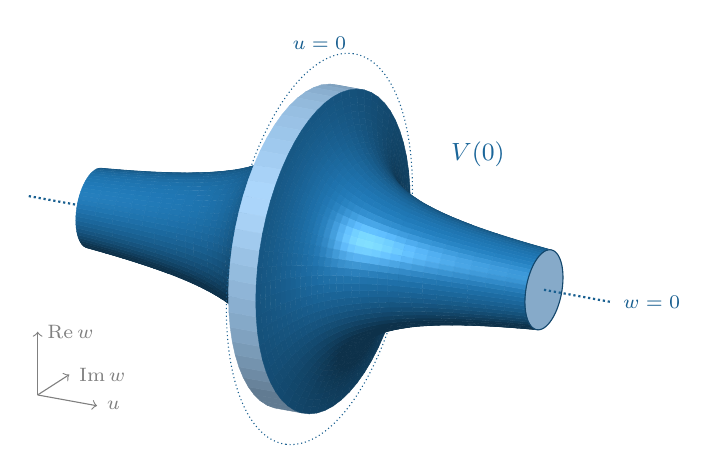
\begin{tikzpicture}[scale=0.95]
\draw[regA!80!black, densely dotted] (0.4458,2.6116) -- (0.506,2.6004) -- (0.5648,2.5821) -- (0.622,2.5567) -- (0.6776,2.5243) -- (0.7313,2.485) -- (0.7829,2.4389) -- (0.8325,2.386) -- (0.8797,2.3267) -- (0.9245,2.261) -- (0.9668,2.189) -- (1.0065,2.1111) -- (1.0434,2.0274) -- (1.0774,1.9381) -- (1.1085,1.8436) -- (1.1365,1.7439) -- (1.1615,1.6395) -- (1.1832,1.5306) -- (1.2017,1.4175) -- (1.2169,1.3005) -- (1.2288,1.18) -- (1.2373,1.0562) -- (1.2424,0.9295) -- (1.2441,0.8003) -- (1.2424,0.6688) -- (1.2373,0.5356) -- (1.2288,0.4009) -- (1.2169,0.265) -- (1.2017,0.1285) -- (1.1832,-0.0084) -- (1.1615,-0.1453) -- (1.1365,-0.2818) -- (1.1085,-0.4175) -- (1.0774,-0.552) -- (1.0434,-0.6851) -- (1.0065,-0.8163) -- (0.9668,-0.9452) -- (0.9245,-1.0715) -- (0.8797,-1.195) -- (0.8325,-1.3151) -- (0.7829,-1.4316) -- (0.7313,-1.5442) -- (0.6776,-1.6526) -- (0.622,-1.7564) -- (0.5648,-1.8555) -- (0.506,-1.9494) -- (0.4458,-2.038) -- (0.3844,-2.121) -- (0.322,-2.1982) -- (0.2587,-2.2694) -- (0.1946,-2.3343) -- (0.13,-2.3929) -- (0.0651,-2.4449) -- (0,-2.4902) -- (-0.0651,-2.5287) -- (-0.13,-2.5602) -- (-0.1946,-2.5847) -- (-0.2587,-2.6022) -- (-0.322,-2.6125) -- (-0.3844,-2.6156) -- (-0.4458,-2.6116);
\draw[regA!80!black, densely dotted, thick] (-3.885,0.7065) -- (-3.002,0.5459);
\filldraw[fill={rgb,255:red,16;green,60;blue,90}, draw={rgb,255:red,16;green,60;blue,90}, line width=0.15pt] (1.1647,-0.0402) -- (1.1378,-0.0431) -- (1.1008,-0.2597) -- (1.126,-0.2671) -- cycle;
\filldraw[fill={rgb,255:red,15;green,59;blue,89}, draw={rgb,255:red,15;green,59;blue,89}, line width=0.15pt] (1.126,-0.2671) -- (1.1008,-0.2597) -- (1.0539,-0.4738) -- (1.0769,-0.4915) -- cycle;
\filldraw[fill={rgb,255:red,16;green,60;blue,91}, draw={rgb,255:red,16;green,60;blue,91}, line width=0.15pt] (1.1927,0.1869) -- (1.1645,0.1736) -- (1.1378,-0.0431) -- (1.1647,-0.0402) -- cycle;
\filldraw[fill={rgb,255:red,15;green,59;blue,89}, draw={rgb,255:red,15;green,59;blue,89}, line width=0.15pt] (1.0769,-0.4915) -- (1.0539,-0.4738) -- (0.9978,-0.6832) -- (1.018,-0.7108) -- cycle;
\filldraw[fill={rgb,255:red,16;green,61;blue,93}, draw={rgb,255:red,16;green,61;blue,93}, line width=0.15pt] (1.2096,0.4115) -- (1.1806,0.3879) -- (1.1645,0.1736) -- (1.1927,0.1869) -- cycle;
\filldraw[fill={rgb,255:red,15;green,58;blue,88}, draw={rgb,255:red,15;green,58;blue,88}, line width=0.15pt] (1.018,-0.7108) -- (0.9978,-0.6832) -- (0.9328,-0.8854) -- (0.95,-0.9228) -- cycle;
\filldraw[fill={rgb,255:red,15;green,58;blue,87}, draw={rgb,255:red,15;green,58;blue,87}, line width=0.15pt] (1.1378,-0.0431) -- (1.1146,-0.0463) -- (1.0793,-0.2531) -- (1.1008,-0.2597) -- cycle;
\filldraw[fill={rgb,255:red,15;green,57;blue,86}, draw={rgb,255:red,15;green,57;blue,86}, line width=0.15pt] (1.1008,-0.2597) -- (1.0793,-0.2531) -- (1.0346,-0.4574) -- (1.0539,-0.4738) -- cycle;
\filldraw[fill={rgb,255:red,16;green,62;blue,94}, draw={rgb,255:red,16;green,62;blue,94}, line width=0.15pt] (1.2153,0.6312) -- (1.186,0.5976) -- (1.1806,0.3879) -- (1.2096,0.4115) -- cycle;
\filldraw[fill={rgb,255:red,15;green,58;blue,88}, draw={rgb,255:red,15;green,58;blue,88}, line width=0.15pt] (1.1645,0.1736) -- (1.1401,0.1604) -- (1.1146,-0.0463) -- (1.1378,-0.0431) -- cycle;
\filldraw[fill={rgb,255:red,15;green,56;blue,85}, draw={rgb,255:red,15;green,56;blue,85}, line width=0.15pt] (1.0539,-0.4738) -- (1.0346,-0.4574) -- (0.981,-0.6572) -- (0.9978,-0.6832) -- cycle;
\filldraw[fill={rgb,255:red,15;green,59;blue,90}, draw={rgb,255:red,15;green,59;blue,90}, line width=0.15pt] (1.1806,0.3879) -- (1.1555,0.365) -- (1.1401,0.1604) -- (1.1645,0.1736) -- cycle;
\filldraw[fill={rgb,255:red,15;green,58;blue,88}, draw={rgb,255:red,15;green,58;blue,88}, line width=0.15pt] (0.95,-0.9228) -- (0.9328,-0.8854) -- (0.8599,-1.0784) -- (0.8735,-1.1249) -- cycle;
\filldraw[fill={rgb,255:red,15;green,56;blue,85}, draw={rgb,255:red,15;green,56;blue,85}, line width=0.15pt] (0.9978,-0.6832) -- (0.981,-0.6572) -- (0.919,-0.8503) -- (0.9328,-0.8854) -- cycle;
\filldraw[fill={rgb,255:red,16;green,63;blue,96}, draw={rgb,255:red,16;green,63;blue,96}, line width=0.15pt] (1.2096,0.8436) -- (1.1806,0.8004) -- (1.186,0.5976) -- (1.2153,0.6312) -- cycle;
\filldraw[fill={rgb,255:red,14;green,55;blue,83}, draw={rgb,255:red,14;green,55;blue,83}, line width=0.15pt] (1.1146,-0.0463) -- (1.0953,-0.05) -- (1.0616,-0.2473) -- (1.0793,-0.2531) -- cycle;
\filldraw[fill={rgb,255:red,14;green,54;blue,82}, draw={rgb,255:red,14;green,54;blue,82}, line width=0.15pt] (1.0793,-0.2531) -- (1.0616,-0.2473) -- (1.019,-0.4423) -- (1.0346,-0.4574) -- cycle;
\filldraw[fill={rgb,255:red,16;green,60;blue,91}, draw={rgb,255:red,16;green,60;blue,91}, line width=0.15pt] (1.186,0.5976) -- (1.1607,0.5652) -- (1.1555,0.365) -- (1.1806,0.3879) -- cycle;
\filldraw[fill={rgb,255:red,15;green,56;blue,85}, draw={rgb,255:red,15;green,56;blue,85}, line width=0.15pt] (1.1401,0.1604) -- (1.1196,0.1474) -- (1.0953,-0.05) -- (1.1146,-0.0463) -- cycle;
\filldraw[fill={rgb,255:red,14;green,54;blue,81}, draw={rgb,255:red,14;green,54;blue,81}, line width=0.15pt] (1.0346,-0.4574) -- (1.019,-0.4423) -- (0.9678,-0.633) -- (0.981,-0.6572) -- cycle;
\filldraw[fill={rgb,255:red,15;green,58;blue,88}, draw={rgb,255:red,15;green,58;blue,88}, line width=0.15pt] (0.8735,-1.1249) -- (0.8599,-1.0784) -- (0.7797,-1.2599) -- (0.7895,-1.3152) -- cycle;
\filldraw[fill={rgb,255:red,15;green,56;blue,85}, draw={rgb,255:red,15;green,56;blue,85}, line width=0.15pt] (0.9328,-0.8854) -- (0.919,-0.8503) -- (0.8494,-1.0344) -- (0.8599,-1.0784) -- cycle;
\filldraw[fill={rgb,255:red,15;green,57;blue,86}, draw={rgb,255:red,15;green,57;blue,86}, line width=0.15pt] (1.1555,0.365) -- (1.1343,0.3426) -- (1.1196,0.1474) -- (1.1401,0.1604) -- cycle;
\filldraw[fill={rgb,255:red,14;green,54;blue,81}, draw={rgb,255:red,14;green,54;blue,81}, line width=0.15pt] (0.981,-0.6572) -- (0.9678,-0.633) -- (0.9086,-0.8172) -- (0.919,-0.8503) -- cycle;
\filldraw[fill={rgb,255:red,16;green,62;blue,93}, draw={rgb,255:red,16;green,62;blue,93}, line width=0.15pt] (1.1806,0.8004) -- (1.1555,0.7587) -- (1.1607,0.5652) -- (1.186,0.5976) -- cycle;
\filldraw[fill={rgb,255:red,17;green,65;blue,98}, draw={rgb,255:red,17;green,65;blue,98}, line width=0.15pt] (1.1927,1.0465) -- (1.1645,0.994) -- (1.1806,0.8004) -- (1.2096,0.8436) -- cycle;
\filldraw[fill={rgb,255:red,14;green,52;blue,79}, draw={rgb,255:red,14;green,52;blue,79}, line width=0.15pt] (1.0953,-0.05) -- (1.08,-0.054) -- (1.0479,-0.2423) -- (1.0616,-0.2473) -- cycle;
\filldraw[fill={rgb,255:red,13;green,52;blue,78}, draw={rgb,255:red,13;green,52;blue,78}, line width=0.15pt] (1.0616,-0.2473) -- (1.0479,-0.2423) -- (1.0071,-0.4284) -- (1.019,-0.4423) -- cycle;
\filldraw[fill={rgb,255:red,15;green,58;blue,88}, draw={rgb,255:red,15;green,58;blue,88}, line width=0.15pt] (1.1607,0.5652) -- (1.1393,0.5337) -- (1.1343,0.3426) -- (1.1555,0.365) -- cycle;
\filldraw[fill={rgb,255:red,14;green,53;blue,81}, draw={rgb,255:red,14;green,53;blue,81}, line width=0.15pt] (1.1196,0.1474) -- (1.1032,0.1344) -- (1.08,-0.054) -- (1.0953,-0.05) -- cycle;
\filldraw[fill={rgb,255:red,13;green,51;blue,77}, draw={rgb,255:red,13;green,51;blue,77}, line width=0.15pt] (1.019,-0.4423) -- (1.0071,-0.4284) -- (0.9583,-0.6104) -- (0.9678,-0.633) -- cycle;
\filldraw[fill={rgb,255:red,15;green,56;blue,85}, draw={rgb,255:red,15;green,56;blue,85}, line width=0.15pt] (0.8599,-1.0784) -- (0.8494,-1.0344) -- (0.7729,-1.2077) -- (0.7797,-1.2599) -- cycle;
\filldraw[fill={rgb,255:red,14;green,53;blue,81}, draw={rgb,255:red,14;green,53;blue,81}, line width=0.15pt] (0.919,-0.8503) -- (0.9086,-0.8172) -- (0.8422,-0.993) -- (0.8494,-1.0344) -- cycle;
\filldraw[fill={rgb,255:red,14;green,55;blue,83}, draw={rgb,255:red,14;green,55;blue,83}, line width=0.15pt] (1.1343,0.3426) -- (1.1172,0.3207) -- (1.1032,0.1344) -- (1.1196,0.1474) -- cycle;
\filldraw[fill={rgb,255:red,15;green,59;blue,89}, draw={rgb,255:red,15;green,59;blue,89}, line width=0.15pt] (0.7895,-1.3152) -- (0.7797,-1.2599) -- (0.6931,-1.4281) -- (0.6988,-1.4913) -- cycle;
\filldraw[fill={rgb,255:red,13;green,51;blue,77}, draw={rgb,255:red,13;green,51;blue,77}, line width=0.15pt] (0.9678,-0.633) -- (0.9583,-0.6104) -- (0.9018,-0.7863) -- (0.9086,-0.8172) -- cycle;
\filldraw[fill={rgb,255:red,16;green,60;blue,91}, draw={rgb,255:red,16;green,60;blue,91}, line width=0.15pt] (1.1555,0.7587) -- (1.1343,0.7183) -- (1.1393,0.5337) -- (1.1607,0.5652) -- cycle;
\filldraw[fill={rgb,255:red,16;green,63;blue,95}, draw={rgb,255:red,16;green,63;blue,95}, line width=0.15pt] (1.1645,0.994) -- (1.1401,0.9435) -- (1.1555,0.7587) -- (1.1806,0.8004) -- cycle;
\filldraw[fill={rgb,255:red,13;green,49;blue,75}, draw={rgb,255:red,13;green,49;blue,75}, line width=0.15pt] (1.08,-0.054) -- (1.0688,-0.0584) -- (1.0381,-0.2381) -- (1.0479,-0.2423) -- cycle;
\filldraw[fill={rgb,255:red,13;green,49;blue,74}, draw={rgb,255:red,13;green,49;blue,74}, line width=0.15pt] (1.0479,-0.2423) -- (1.0381,-0.2381) -- (0.9992,-0.4158) -- (1.0071,-0.4284) -- cycle;
\filldraw[fill={rgb,255:red,15;green,56;blue,85}, draw={rgb,255:red,15;green,56;blue,85}, line width=0.15pt] (1.1393,0.5337) -- (1.1219,0.503) -- (1.1172,0.3207) -- (1.1343,0.3426) -- cycle;
\filldraw[fill={rgb,255:red,13;green,51;blue,76}, draw={rgb,255:red,13;green,51;blue,76}, line width=0.15pt] (1.1032,0.1344) -- (1.0909,0.1213) -- (1.0688,-0.0584) -- (1.08,-0.054) -- cycle;
\filldraw[fill={rgb,255:red,17;green,66;blue,100}, draw={rgb,255:red,17;green,66;blue,100}, line width=0.15pt] (1.1647,1.2375) -- (1.1378,1.1763) -- (1.1645,0.994) -- (1.1927,1.0465) -- cycle;
\filldraw[fill={rgb,255:red,13;green,49;blue,74}, draw={rgb,255:red,13;green,49;blue,74}, line width=0.15pt] (1.0071,-0.4284) -- (0.9992,-0.4158) -- (0.9526,-0.5895) -- (0.9583,-0.6104) -- cycle;
\filldraw[fill={rgb,255:red,14;green,54;blue,81}, draw={rgb,255:red,14;green,54;blue,81}, line width=0.15pt] (0.8494,-1.0344) -- (0.8422,-0.993) -- (0.7691,-1.1584) -- (0.7729,-1.2077) -- cycle;
\filldraw[fill={rgb,255:red,13;green,50;blue,76}, draw={rgb,255:red,13;green,50;blue,76}, line width=0.15pt] (0.9086,-0.8172) -- (0.9018,-0.7863) -- (0.8384,-0.954) -- (0.8422,-0.993) -- cycle;
\filldraw[fill={rgb,255:red,14;green,52;blue,79}, draw={rgb,255:red,14;green,52;blue,79}, line width=0.15pt] (1.1172,0.3207) -- (1.1043,0.2992) -- (1.0909,0.1213) -- (1.1032,0.1344) -- cycle;
\filldraw[fill={rgb,255:red,15;green,56;blue,85}, draw={rgb,255:red,15;green,56;blue,85}, line width=0.15pt] (0.7797,-1.2599) -- (0.7729,-1.2077) -- (0.6903,-1.3682) -- (0.6931,-1.4281) -- cycle;
\filldraw[fill={rgb,255:red,13;green,49;blue,74}, draw={rgb,255:red,13;green,49;blue,74}, line width=0.15pt] (-2.843,-0.0603) -- (-3.1056,0.0138) -- (-3.1293,0.0227) -- (-2.8678,-0.051) -- cycle;
\filldraw[fill={rgb,255:red,13;green,49;blue,74}, draw={rgb,255:red,13;green,49;blue,74}, line width=0.15pt] (0.9583,-0.6104) -- (0.9526,-0.5895) -- (0.8987,-0.7573) -- (0.9018,-0.7863) -- cycle;
\filldraw[fill={rgb,255:red,15;green,58;blue,87}, draw={rgb,255:red,15;green,58;blue,87}, line width=0.15pt] (1.1343,0.7183) -- (1.1172,0.6793) -- (1.1219,0.503) -- (1.1393,0.5337) -- cycle;
\filldraw[fill={rgb,255:red,16;green,61;blue,93}, draw={rgb,255:red,16;green,61;blue,93}, line width=0.15pt] (1.1401,0.9435) -- (1.1196,0.8947) -- (1.1343,0.7183) -- (1.1555,0.7587) -- cycle;
\filldraw[fill={rgb,255:red,13;green,49;blue,74}, draw={rgb,255:red,13;green,49;blue,74}, line width=0.15pt] (1.0688,-0.0584) -- (1.0618,-0.0634) -- (1.0325,-0.2349) -- (1.0381,-0.2381) -- cycle;
\filldraw[fill={rgb,255:red,22;green,84;blue,128}, draw={rgb,255:red,22;green,84;blue,128}, line width=0.15pt] (-2.679,1.0553) -- (-2.9491,1.0785) -- (-2.9233,1.0812) -- (-2.652,1.0581) -- cycle;
\filldraw[fill={rgb,255:red,14;green,54;blue,81}, draw={rgb,255:red,14;green,54;blue,81}, line width=0.15pt] (1.1219,0.503) -- (1.1088,0.4732) -- (1.1043,0.2992) -- (1.1172,0.3207) -- cycle;
\filldraw[fill={rgb,255:red,13;green,49;blue,74}, draw={rgb,255:red,13;green,49;blue,74}, line width=0.15pt] (1.0381,-0.2381) -- (1.0325,-0.2349) -- (0.9954,-0.4044) -- (0.9992,-0.4158) -- cycle;
\filldraw[fill={rgb,255:red,15;green,59;blue,89}, draw={rgb,255:red,15;green,59;blue,89}, line width=0.15pt] (0.6988,-1.4913) -- (0.6931,-1.4281) -- (0.6012,-1.581) -- (0.6025,-1.6515) -- cycle;
\filldraw[fill={rgb,255:red,13;green,49;blue,74}, draw={rgb,255:red,13;green,49;blue,74}, line width=0.15pt] (1.0909,0.1213) -- (1.0829,0.1082) -- (1.0618,-0.0634) -- (1.0688,-0.0584) -- cycle;
\filldraw[fill={rgb,255:red,17;green,65;blue,98}, draw={rgb,255:red,17;green,65;blue,98}, line width=0.15pt] (1.1378,1.1763) -- (1.1146,1.1174) -- (1.1401,0.9435) -- (1.1645,0.994) -- cycle;
\filldraw[fill={rgb,255:red,13;green,49;blue,74}, draw={rgb,255:red,13;green,49;blue,74}, line width=0.15pt] (0.9992,-0.4158) -- (0.9954,-0.4044) -- (0.9509,-0.5702) -- (0.9526,-0.5895) -- cycle;
\filldraw[fill={rgb,255:red,13;green,51;blue,77}, draw={rgb,255:red,13;green,51;blue,77}, line width=0.15pt] (0.8422,-0.993) -- (0.8384,-0.954) -- (0.7687,-1.1118) -- (0.7691,-1.1584) -- cycle;
\filldraw[fill={rgb,255:red,13;green,49;blue,74}, draw={rgb,255:red,13;green,49;blue,74}, line width=0.15pt] (-2.8678,-0.051) -- (-3.1293,0.0227) -- (-3.1517,0.0374) -- (-2.8913,-0.0356) -- cycle;
\filldraw[fill={rgb,255:red,13;green,49;blue,74}, draw={rgb,255:red,13;green,49;blue,74}, line width=0.15pt] (0.9018,-0.7863) -- (0.8987,-0.7573) -- (0.8382,-0.9174) -- (0.8384,-0.954) -- cycle;
\filldraw[fill={rgb,255:red,13;green,49;blue,74}, draw={rgb,255:red,13;green,49;blue,74}, line width=0.15pt] (1.1043,0.2992) -- (1.0957,0.2779) -- (1.0829,0.1082) -- (1.0909,0.1213) -- cycle;
\filldraw[fill={rgb,255:red,14;green,54;blue,81}, draw={rgb,255:red,14;green,54;blue,81}, line width=0.15pt] (0.7729,-1.2077) -- (0.7691,-1.1584) -- (0.6903,-1.3115) -- (0.6903,-1.3682) -- cycle;
\filldraw[fill={rgb,255:red,24;green,91;blue,138}, draw={rgb,255:red,24;green,91;blue,138}, line width=0.15pt] (-2.7066,1.0463) -- (-2.9754,1.0699) -- (-2.9491,1.0785) -- (-2.679,1.0553) -- cycle;
\filldraw[fill={rgb,255:red,13;green,49;blue,74}, draw={rgb,255:red,13;green,49;blue,74}, line width=0.15pt] (0.9526,-0.5895) -- (0.9509,-0.5702) -- (0.8995,-0.7304) -- (0.8987,-0.7573) -- cycle;
\filldraw[fill={rgb,255:red,14;green,56;blue,84}, draw={rgb,255:red,14;green,56;blue,84}, line width=0.15pt] (1.1172,0.6793) -- (1.1043,0.6414) -- (1.1088,0.4732) -- (1.1219,0.503) -- cycle;
\filldraw[fill={rgb,255:red,18;green,67;blue,102}, draw={rgb,255:red,18;green,67;blue,102}, line width=0.15pt] (1.126,1.4146) -- (1.1008,1.3453) -- (1.1378,1.1763) -- (1.1647,1.2375) -- cycle;
\filldraw[fill={rgb,255:red,16;green,60;blue,90}, draw={rgb,255:red,16;green,60;blue,90}, line width=0.15pt] (1.1196,0.8947) -- (1.1032,0.8476) -- (1.1172,0.6793) -- (1.1343,0.7183) -- cycle;
\filldraw[fill={rgb,255:red,15;green,57;blue,86}, draw={rgb,255:red,15;green,57;blue,86}, line width=0.15pt] (0.6931,-1.4281) -- (0.6903,-1.3682) -- (0.6025,-1.5141) -- (0.6012,-1.581) -- cycle;
\filldraw[fill={rgb,255:red,13;green,49;blue,74}, draw={rgb,255:red,13;green,49;blue,74}, line width=0.15pt] (-2.8913,-0.0356) -- (-3.1517,0.0374) -- (-3.1724,0.0576) -- (-2.913,-0.0144) -- cycle;
\filldraw[fill={rgb,255:red,13;green,49;blue,74}, draw={rgb,255:red,13;green,49;blue,74}, line width=0.15pt] (1.0618,-0.0634) -- (1.0592,-0.0688) -- (1.0312,-0.2325) -- (1.0325,-0.2349) -- cycle;
\filldraw[fill={rgb,255:red,13;green,51;blue,77}, draw={rgb,255:red,13;green,51;blue,77}, line width=0.15pt] (1.1088,0.4732) -- (1.1,0.444) -- (1.0957,0.2779) -- (1.1043,0.2992) -- cycle;
\filldraw[fill={rgb,255:red,13;green,49;blue,74}, draw={rgb,255:red,13;green,49;blue,74}, line width=0.15pt] (1.0325,-0.2349) -- (1.0312,-0.2325) -- (0.9958,-0.3943) -- (0.9954,-0.4044) -- cycle;
\filldraw[fill={rgb,255:red,16;green,63;blue,96}, draw={rgb,255:red,16;green,63;blue,96}, line width=0.15pt] (1.1146,1.1174) -- (1.0953,1.0607) -- (1.1196,0.8947) -- (1.1401,0.9435) -- cycle;
\filldraw[fill={rgb,255:red,13;green,49;blue,74}, draw={rgb,255:red,13;green,49;blue,74}, line width=0.15pt] (1.0829,0.1082) -- (1.0793,0.0949) -- (1.0592,-0.0688) -- (1.0618,-0.0634) -- cycle;
\filldraw[fill={rgb,255:red,25;green,97;blue,147}, draw={rgb,255:red,25;green,97;blue,147}, line width=0.15pt] (-2.7344,1.0312) -- (-3.002,1.0556) -- (-2.9754,1.0699) -- (-2.7066,1.0463) -- cycle;
\filldraw[fill={rgb,255:red,13;green,49;blue,74}, draw={rgb,255:red,13;green,49;blue,74}, line width=0.15pt] (0.8384,-0.954) -- (0.8382,-0.9174) -- (0.7717,-1.068) -- (0.7687,-1.1118) -- cycle;
\filldraw[fill={rgb,255:red,13;green,49;blue,74}, draw={rgb,255:red,13;green,49;blue,74}, line width=0.15pt] (0.9954,-0.4044) -- (0.9958,-0.3943) -- (0.9533,-0.5525) -- (0.9509,-0.5702) -- cycle;
\filldraw[fill={rgb,255:red,13;green,49;blue,74}, draw={rgb,255:red,13;green,49;blue,74}, line width=0.15pt] (-2.6044,-0.1313) -- (-2.843,-0.0603) -- (-2.8678,-0.051) -- (-2.6305,-0.1215) -- cycle;
\filldraw[fill={rgb,255:red,13;green,49;blue,74}, draw={rgb,255:red,13;green,49;blue,74}, line width=0.15pt] (0.8987,-0.7573) -- (0.8995,-0.7304) -- (0.8417,-0.8832) -- (0.8382,-0.9174) -- cycle;
\filldraw[fill={rgb,255:red,13;green,51;blue,77}, draw={rgb,255:red,13;green,51;blue,77}, line width=0.15pt] (0.7691,-1.1584) -- (0.7687,-1.1118) -- (0.6935,-1.258) -- (0.6903,-1.3115) -- cycle;
\filldraw[fill={rgb,255:red,13;green,49;blue,74}, draw={rgb,255:red,13;green,49;blue,74}, line width=0.15pt] (1.0957,0.2779) -- (1.0915,0.2569) -- (1.0793,0.0949) -- (1.0829,0.1082) -- cycle;
\filldraw[fill={rgb,255:red,13;green,49;blue,74}, draw={rgb,255:red,13;green,49;blue,74}, line width=0.15pt] (-2.913,-0.0144) -- (-3.1724,0.0576) -- (-3.1912,0.0832) -- (-2.9327,0.0125) -- cycle;
\filldraw[fill={rgb,255:red,22;green,84;blue,127}, draw={rgb,255:red,22;green,84;blue,127}, line width=0.15pt] (-2.4326,1.0376) -- (-2.679,1.0553) -- (-2.652,1.0581) -- (-2.4043,1.0406) -- cycle;
\filldraw[fill={rgb,255:red,17;green,66;blue,100}, draw={rgb,255:red,17;green,66;blue,100}, line width=0.15pt] (1.1008,1.3453) -- (1.0793,1.2788) -- (1.1146,1.1174) -- (1.1378,1.1763) -- cycle;
\filldraw[fill={rgb,255:red,16;green,60;blue,90}, draw={rgb,255:red,16;green,60;blue,90}, line width=0.15pt] (0.6025,-1.6515) -- (0.6012,-1.581) -- (0.5049,-1.717) -- (0.5016,-1.794) -- cycle;
\filldraw[fill={rgb,255:red,13;green,49;blue,74}, draw={rgb,255:red,13;green,49;blue,74}, line width=0.15pt] (0.9509,-0.5702) -- (0.9533,-0.5525) -- (0.9043,-0.7054) -- (0.8995,-0.7304) -- cycle;
\filldraw[fill={rgb,255:red,14;green,53;blue,80}, draw={rgb,255:red,14;green,53;blue,80}, line width=0.15pt] (1.1043,0.6414) -- (1.0957,0.6046) -- (1.1,0.444) -- (1.1088,0.4732) -- cycle;
\filldraw[fill={rgb,255:red,15;green,58;blue,87}, draw={rgb,255:red,15;green,58;blue,87}, line width=0.15pt] (1.1032,0.8476) -- (1.0909,0.802) -- (1.1043,0.6414) -- (1.1172,0.6793) -- cycle;
\filldraw[fill={rgb,255:red,27;green,103;blue,155}, draw={rgb,255:red,27;green,103;blue,155}, line width=0.15pt] (-2.7623,1.0104) -- (-3.0286,1.0356) -- (-3.002,1.0556) -- (-2.7344,1.0312) -- cycle;
\filldraw[fill={rgb,255:red,14;green,54;blue,82}, draw={rgb,255:red,14;green,54;blue,82}, line width=0.15pt] (0.6903,-1.3682) -- (0.6903,-1.3115) -- (0.6066,-1.4508) -- (0.6025,-1.5141) -- cycle;
\filldraw[fill={rgb,255:red,13;green,49;blue,74}, draw={rgb,255:red,13;green,49;blue,74}, line width=0.15pt] (-2.6305,-0.1215) -- (-2.8678,-0.051) -- (-2.8913,-0.0356) -- (-2.655,-0.1054) -- cycle;
\filldraw[fill={rgb,255:red,13;green,49;blue,74}, draw={rgb,255:red,13;green,49;blue,74}, line width=0.15pt] (1.1,0.444) -- (1.0956,0.4154) -- (1.0915,0.2569) -- (1.0957,0.2779) -- cycle;
\filldraw[fill={rgb,255:red,16;green,62;blue,93}, draw={rgb,255:red,16;green,62;blue,93}, line width=0.15pt] (1.0953,1.0607) -- (1.08,1.0061) -- (1.1032,0.8476) -- (1.1196,0.8947) -- cycle;
\filldraw[fill={rgb,255:red,14;green,55;blue,83}, draw={rgb,255:red,14;green,55;blue,83}, line width=0.15pt] (-2.9327,0.0125) -- (-3.1912,0.0832) -- (-3.208,0.1139) -- (-2.9503,0.0446) -- cycle;
\filldraw[fill={rgb,255:red,13;green,49;blue,74}, draw={rgb,255:red,13;green,49;blue,74}, line width=0.15pt] (0.8382,-0.9174) -- (0.8417,-0.8832) -- (0.7782,-1.0269) -- (0.7717,-1.068) -- cycle;
\filldraw[fill={rgb,255:red,24;green,91;blue,137}, draw={rgb,255:red,24;green,91;blue,137}, line width=0.15pt] (-2.4615,1.0282) -- (-2.7066,1.0463) -- (-2.679,1.0553) -- (-2.4326,1.0376) -- cycle;
\filldraw[fill={rgb,255:red,13;green,49;blue,74}, draw={rgb,255:red,13;green,49;blue,74}, line width=0.15pt] (0.7687,-1.1118) -- (0.7717,-1.068) -- (0.6999,-1.2076) -- (0.6935,-1.258) -- cycle;
\filldraw[fill={rgb,255:red,13;green,49;blue,74}, draw={rgb,255:red,13;green,49;blue,74}, line width=0.15pt] (0.8995,-0.7304) -- (0.9043,-0.7054) -- (0.8491,-0.8512) -- (0.8417,-0.8832) -- cycle;
\filldraw[fill={rgb,255:red,28;green,108;blue,163}, draw={rgb,255:red,28;green,108;blue,163}, line width=0.15pt] (-2.7899,0.9839) -- (-3.055,1.0104) -- (-3.0286,1.0356) -- (-2.7623,1.0104) -- cycle;
\filldraw[fill={rgb,255:red,17;green,65;blue,98}, draw={rgb,255:red,17;green,65;blue,98}, line width=0.15pt] (1.0793,1.2788) -- (1.0616,1.2147) -- (1.0953,1.0607) -- (1.1146,1.1174) -- cycle;
\filldraw[fill={rgb,255:red,15;green,58;blue,87}, draw={rgb,255:red,15;green,58;blue,87}, line width=0.15pt] (0.6012,-1.581) -- (0.6025,-1.5141) -- (0.5106,-1.6439) -- (0.5049,-1.717) -- cycle;
\filldraw[fill={rgb,255:red,18;green,69;blue,104}, draw={rgb,255:red,18;green,69;blue,104}, line width=0.15pt] (1.0769,1.5758) -- (1.0539,1.4992) -- (1.1008,1.3453) -- (1.126,1.4146) -- cycle;
\filldraw[fill={rgb,255:red,13;green,49;blue,74}, draw={rgb,255:red,13;green,49;blue,74}, line width=0.15pt] (-2.655,-0.1054) -- (-2.8913,-0.0356) -- (-2.913,-0.0144) -- (-2.6778,-0.0831) -- cycle;
\filldraw[fill={rgb,255:red,16;green,62;blue,94}, draw={rgb,255:red,16;green,62;blue,94}, line width=0.15pt] (-2.9503,0.0446) -- (-3.208,0.1139) -- (-3.2225,0.1493) -- (-2.9655,0.0817) -- cycle;
\filldraw[fill={rgb,255:red,14;green,55;blue,84}, draw={rgb,255:red,14;green,55;blue,84}, line width=0.15pt] (1.0909,0.802) -- (1.0829,0.7579) -- (1.0957,0.6046) -- (1.1043,0.6414) -- cycle;
\filldraw[fill={rgb,255:red,13;green,50;blue,76}, draw={rgb,255:red,13;green,50;blue,76}, line width=0.15pt] (1.0957,0.6046) -- (1.0915,0.5687) -- (1.0956,0.4154) -- (1.1,0.444) -- cycle;
\filldraw[fill={rgb,255:red,13;green,52;blue,78}, draw={rgb,255:red,13;green,52;blue,78}, line width=0.15pt] (0.6903,-1.3115) -- (0.6935,-1.258) -- (0.6136,-1.3909) -- (0.6066,-1.4508) -- cycle;
\filldraw[fill={rgb,255:red,13;green,49;blue,74}, draw={rgb,255:red,13;green,49;blue,74}, line width=0.15pt] (-2.3878,-0.1996) -- (-2.6044,-0.1313) -- (-2.6305,-0.1215) -- (-2.4152,-0.1893) -- cycle;
\filldraw[fill={rgb,255:red,25;green,97;blue,146}, draw={rgb,255:red,25;green,97;blue,146}, line width=0.15pt] (-2.4907,1.0124) -- (-2.7344,1.0312) -- (-2.7066,1.0463) -- (-2.4615,1.0282) -- cycle;
\filldraw[fill={rgb,255:red,16;green,60;blue,90}, draw={rgb,255:red,16;green,60;blue,90}, line width=0.15pt] (1.08,1.0061) -- (1.0688,0.9533) -- (1.0909,0.802) -- (1.1032,0.8476) -- cycle;
\filldraw[fill={rgb,255:red,29;green,112;blue,169}, draw={rgb,255:red,29;green,112;blue,169}, line width=0.15pt] (-2.8169,0.9521) -- (-3.0807,0.98) -- (-3.055,1.0104) -- (-2.7899,0.9839) -- cycle;
\filldraw[fill={rgb,255:red,22;green,84;blue,126}, draw={rgb,255:red,22;green,84;blue,126}, line width=0.15pt] (-2.2078,1.0252) -- (-2.4326,1.0376) -- (-2.4043,1.0406) -- (-2.1782,1.0283) -- cycle;
\filldraw[fill={rgb,255:red,13;green,49;blue,74}, draw={rgb,255:red,13;green,49;blue,74}, line width=0.15pt] (0.8417,-0.8832) -- (0.8491,-0.8512) -- (0.7885,-0.9884) -- (0.7782,-1.0269) -- cycle;
\filldraw[fill={rgb,255:red,18;green,70;blue,106}, draw={rgb,255:red,18;green,70;blue,106}, line width=0.15pt] (-2.9655,0.0817) -- (-3.2225,0.1493) -- (-3.2346,0.189) -- (-2.9782,0.1233) -- cycle;
\filldraw[fill={rgb,255:red,13;green,49;blue,74}, draw={rgb,255:red,13;green,49;blue,74}, line width=0.15pt] (-2.6778,-0.0831) -- (-2.913,-0.0144) -- (-2.9327,0.0125) -- (-2.6984,-0.055) -- cycle;
\filldraw[fill={rgb,255:red,13;green,49;blue,74}, draw={rgb,255:red,13;green,49;blue,74}, line width=0.15pt] (0.7717,-1.068) -- (0.7782,-1.0269) -- (0.7097,-1.1601) -- (0.6999,-1.2076) -- cycle;
\filldraw[fill={rgb,255:red,18;green,68;blue,103}, draw={rgb,255:red,18;green,68;blue,103}, line width=0.15pt] (1.0539,1.4992) -- (1.0346,1.4256) -- (1.0793,1.2788) -- (1.1008,1.3453) -- cycle;
\filldraw[fill={rgb,255:red,30;green,116;blue,175}, draw={rgb,255:red,30;green,116;blue,175}, line width=0.15pt] (-2.843,0.9153) -- (-3.1056,0.9449) -- (-3.0807,0.98) -- (-2.8169,0.9521) -- cycle;
\filldraw[fill={rgb,255:red,14;green,55;blue,83}, draw={rgb,255:red,14;green,55;blue,83}, line width=0.15pt] (0.6025,-1.5141) -- (0.6066,-1.4508) -- (0.5189,-1.5746) -- (0.5106,-1.6439) -- cycle;
\filldraw[fill={rgb,255:red,17;green,64;blue,96}, draw={rgb,255:red,17;green,64;blue,96}, line width=0.15pt] (1.0616,1.2147) -- (1.0479,1.153) -- (1.08,1.0061) -- (1.0953,1.0607) -- cycle;
\filldraw[fill={rgb,255:red,13;green,49;blue,74}, draw={rgb,255:red,13;green,49;blue,74}, line width=0.15pt] (-2.4152,-0.1893) -- (-2.6305,-0.1215) -- (-2.655,-0.1054) -- (-2.4409,-0.1724) -- cycle;
\filldraw[fill={rgb,255:red,27;green,102;blue,155}, draw={rgb,255:red,27;green,102;blue,155}, line width=0.15pt] (-2.5199,0.9906) -- (-2.7623,1.0104) -- (-2.7344,1.0312) -- (-2.4907,1.0124) -- cycle;
\filldraw[fill={rgb,255:red,14;green,53;blue,80}, draw={rgb,255:red,14;green,53;blue,80}, line width=0.15pt] (1.0829,0.7579) -- (1.0793,0.715) -- (1.0915,0.5687) -- (1.0957,0.6046) -- cycle;
\filldraw[fill={rgb,255:red,13;green,49;blue,74}, draw={rgb,255:red,13;green,49;blue,74}, line width=0.15pt] (0.6935,-1.258) -- (0.6999,-1.2076) -- (0.6236,-1.3344) -- (0.6136,-1.3909) -- cycle;
\filldraw[fill={rgb,255:red,16;green,60;blue,91}, draw={rgb,255:red,16;green,60;blue,91}, line width=0.15pt] (0.5016,-1.794) -- (0.5049,-1.717) -- (0.4052,-1.8345) -- (0.3972,-1.9172) -- cycle;
\filldraw[fill={rgb,255:red,20;green,77;blue,117}, draw={rgb,255:red,20;green,77;blue,117}, line width=0.15pt] (-2.9782,0.1233) -- (-3.2346,0.189) -- (-3.2442,0.2327) -- (-2.9882,0.1691) -- cycle;
\filldraw[fill={rgb,255:red,13;green,49;blue,74}, draw={rgb,255:red,13;green,49;blue,74}, line width=0.15pt] (1.0915,0.5687) -- (1.0921,0.5336) -- (1.096,0.3873) -- (1.0956,0.4154) -- cycle;
\filldraw[fill={rgb,255:red,24;green,90;blue,136}, draw={rgb,255:red,24;green,90;blue,136}, line width=0.15pt] (-2.2381,1.0153) -- (-2.4615,1.0282) -- (-2.4326,1.0376) -- (-2.2078,1.0252) -- cycle;
\filldraw[fill={rgb,255:red,15;green,58;blue,87}, draw={rgb,255:red,15;green,58;blue,87}, line width=0.15pt] (1.0688,0.9533) -- (1.0618,0.9022) -- (1.0829,0.7579) -- (1.0909,0.802) -- cycle;
\filldraw[fill={rgb,255:red,14;green,54;blue,82}, draw={rgb,255:red,14;green,54;blue,82}, line width=0.15pt] (-2.6984,-0.055) -- (-2.9327,0.0125) -- (-2.9503,0.0446) -- (-2.7169,-0.0214) -- cycle;
\filldraw[fill={rgb,255:red,31;green,119;blue,179}, draw={rgb,255:red,31;green,119;blue,179}, line width=0.15pt] (-2.8678,0.8739) -- (-3.1293,0.9054) -- (-3.1056,0.9449) -- (-2.843,0.9153) -- cycle;
\filldraw[fill={rgb,255:red,22;green,84;blue,128}, draw={rgb,255:red,22;green,84;blue,128}, line width=0.15pt] (-2.9882,0.1691) -- (-3.2442,0.2327) -- (-3.2511,0.2798) -- (-2.9954,0.2184) -- cycle;
\filldraw[fill={rgb,255:red,13;green,49;blue,74}, draw={rgb,255:red,13;green,49;blue,74}, line width=0.15pt] (-2.1913,-0.2656) -- (-2.3878,-0.1996) -- (-2.4152,-0.1893) -- (-2.2199,-0.2548) -- cycle;
\filldraw[fill={rgb,255:red,13;green,49;blue,74}, draw={rgb,255:red,13;green,49;blue,74}, line width=0.15pt] (0.8491,-0.8512) -- (0.8607,-0.8216) -- (0.8029,-0.9525) -- (0.7885,-0.9884) -- cycle;
\filldraw[fill={rgb,255:red,28;green,107;blue,162}, draw={rgb,255:red,28;green,107;blue,162}, line width=0.15pt] (-2.5488,0.9628) -- (-2.7899,0.9839) -- (-2.7623,1.0104) -- (-2.5199,0.9906) -- cycle;
\filldraw[fill={rgb,255:red,13;green,49;blue,74}, draw={rgb,255:red,13;green,49;blue,74}, line width=0.15pt] (-2.4409,-0.1724) -- (-2.655,-0.1054) -- (-2.6778,-0.0831) -- (-2.4647,-0.1491) -- cycle;
\filldraw[fill={rgb,255:red,13;green,49;blue,74}, draw={rgb,255:red,13;green,49;blue,74}, line width=0.15pt] (0.7782,-1.0269) -- (0.7885,-0.9884) -- (0.7231,-1.1155) -- (0.7097,-1.1601) -- cycle;
\filldraw[fill={rgb,255:red,17;green,67;blue,101}, draw={rgb,255:red,17;green,67;blue,101}, line width=0.15pt] (1.0346,1.4256) -- (1.019,1.3549) -- (1.0616,1.2147) -- (1.0793,1.2788) -- cycle;
\filldraw[fill={rgb,255:red,14;green,52;blue,79}, draw={rgb,255:red,14;green,52;blue,79}, line width=0.15pt] (0.6066,-1.4508) -- (0.6136,-1.3909) -- (0.5298,-1.5091) -- (0.5189,-1.5746) -- cycle;
\filldraw[fill={rgb,255:red,32;green,121;blue,183}, draw={rgb,255:red,32;green,121;blue,183}, line width=0.15pt] (-2.8913,0.8284) -- (-3.1517,0.862) -- (-3.1293,0.9054) -- (-2.8678,0.8739) -- cycle;
\filldraw[fill={rgb,255:red,16;green,62;blue,94}, draw={rgb,255:red,16;green,62;blue,94}, line width=0.15pt] (1.0479,1.153) -- (1.0381,1.0935) -- (1.0688,0.9533) -- (1.08,1.0061) -- cycle;
\filldraw[fill={rgb,255:red,15;green,58;blue,88}, draw={rgb,255:red,15;green,58;blue,88}, line width=0.15pt] (0.5049,-1.717) -- (0.5106,-1.6439) -- (0.4155,-1.7561) -- (0.4052,-1.8345) -- cycle;
\filldraw[fill={rgb,255:red,16;green,62;blue,94}, draw={rgb,255:red,16;green,62;blue,94}, line width=0.15pt] (-2.7169,-0.0214) -- (-2.9503,0.0446) -- (-2.9655,0.0817) -- (-2.7328,0.0175) -- cycle;
\filldraw[fill={rgb,255:red,22;green,83;blue,126}, draw={rgb,255:red,22;green,83;blue,126}, line width=0.15pt] (-2.0027,1.0177) -- (-2.2078,1.0252) -- (-2.1782,1.0283) -- (-1.9717,1.021) -- cycle;
\filldraw[fill={rgb,255:red,24;green,91;blue,138}, draw={rgb,255:red,24;green,91;blue,138}, line width=0.15pt] (-2.9954,0.2184) -- (-3.2511,0.2798) -- (-3.2552,0.3298) -- (-2.9998,0.2708) -- cycle;
\filldraw[fill={rgb,255:red,25;green,96;blue,146}, draw={rgb,255:red,25;green,96;blue,146}, line width=0.15pt] (-2.2687,0.9988) -- (-2.4907,1.0124) -- (-2.4615,1.0282) -- (-2.2381,1.0153) -- cycle;
\filldraw[fill={rgb,255:red,13;green,49;blue,74}, draw={rgb,255:red,13;green,49;blue,74}, line width=0.15pt] (0.6999,-1.2076) -- (0.7097,-1.1601) -- (0.6369,-1.2811) -- (0.6236,-1.3344) -- cycle;
\filldraw[fill={rgb,255:red,13;green,50;blue,75}, draw={rgb,255:red,13;green,50;blue,75}, line width=0.15pt] (1.0793,0.715) -- (1.0804,0.6732) -- (1.0921,0.5336) -- (1.0915,0.5687) -- cycle;
\filldraw[fill={rgb,255:red,18;green,70;blue,106}, draw={rgb,255:red,18;green,70;blue,106}, line width=0.15pt] (1.018,1.7195) -- (0.9978,1.6363) -- (1.0539,1.4992) -- (1.0769,1.5758) -- cycle;
\filldraw[fill={rgb,255:red,33;green,123;blue,186}, draw={rgb,255:red,33;green,123;blue,186}, line width=0.15pt] (-2.913,0.7793) -- (-3.1724,0.8151) -- (-3.1517,0.862) -- (-2.8913,0.8284) -- cycle;
\filldraw[fill={rgb,255:red,14;green,55;blue,84}, draw={rgb,255:red,14;green,55;blue,84}, line width=0.15pt] (1.0618,0.9022) -- (1.0592,0.8527) -- (1.0793,0.715) -- (1.0829,0.7579) -- cycle;
\filldraw[fill={rgb,255:red,29;green,112;blue,169}, draw={rgb,255:red,29;green,112;blue,169}, line width=0.15pt] (-2.5771,0.9295) -- (-2.8169,0.9521) -- (-2.7899,0.9839) -- (-2.5488,0.9628) -- cycle;
\filldraw[fill={rgb,255:red,25;green,97;blue,147}, draw={rgb,255:red,25;green,97;blue,147}, line width=0.15pt] (-2.9998,0.2708) -- (-3.2552,0.3298) -- (-3.2566,0.3822) -- (-3.0012,0.3257) -- cycle;
\filldraw[fill={rgb,255:red,13;green,49;blue,74}, draw={rgb,255:red,13;green,49;blue,74}, line width=0.15pt] (-2.4647,-0.1491) -- (-2.6778,-0.0831) -- (-2.6984,-0.055) -- (-2.4864,-0.1197) -- cycle;
\filldraw[fill={rgb,255:red,13;green,49;blue,74}, draw={rgb,255:red,13;green,49;blue,74}, line width=0.15pt] (-2.2199,-0.2548) -- (-2.4152,-0.1893) -- (-2.4409,-0.1724) -- (-2.2469,-0.2371) -- cycle;
\filldraw[fill={rgb,255:red,35;green,126;blue,188}, draw={rgb,255:red,35;green,126;blue,188}, line width=0.15pt] (-2.9327,0.727) -- (-3.1912,0.7652) -- (-3.1724,0.8151) -- (-2.913,0.7793) -- cycle;
\filldraw[fill={rgb,255:red,18;green,70;blue,105}, draw={rgb,255:red,18;green,70;blue,105}, line width=0.15pt] (-2.7328,0.0175) -- (-2.9655,0.0817) -- (-2.9782,0.1233) -- (-2.7461,0.0611) -- cycle;
\filldraw[fill={rgb,255:red,27;green,103;blue,156}, draw={rgb,255:red,27;green,103;blue,156}, line width=0.15pt] (-3.0012,0.3257) -- (-3.2566,0.3822) -- (-3.2552,0.4363) -- (-2.9998,0.3824) -- cycle;
\filldraw[fill={rgb,255:red,17;green,66;blue,100}, draw={rgb,255:red,17;green,66;blue,100}, line width=0.15pt] (1.019,1.3549) -- (1.0071,1.2868) -- (1.0479,1.153) -- (1.0616,1.2147) -- cycle;
\filldraw[fill={rgb,255:red,13;green,49;blue,74}, draw={rgb,255:red,13;green,49;blue,74}, line width=0.15pt] (0.7885,-0.9884) -- (0.8029,-0.9525) -- (0.7405,-1.0738) -- (0.7231,-1.1155) -- cycle;
\filldraw[fill={rgb,255:red,13;green,49;blue,75}, draw={rgb,255:red,13;green,49;blue,75}, line width=0.15pt] (0.6136,-1.3909) -- (0.6236,-1.3344) -- (0.5437,-1.4472) -- (0.5298,-1.5091) -- cycle;
\filldraw[fill={rgb,255:red,37;green,127;blue,189}, draw={rgb,255:red,37;green,127;blue,189}, line width=0.15pt] (-2.9503,0.6723) -- (-3.208,0.713) -- (-3.1912,0.7652) -- (-2.9327,0.727) -- cycle;
\filldraw[fill={rgb,255:red,16;green,60;blue,91}, draw={rgb,255:red,16;green,60;blue,91}, line width=0.15pt] (1.0381,1.0935) -- (1.0325,1.0361) -- (1.0618,0.9022) -- (1.0688,0.9533) -- cycle;
\filldraw[fill={rgb,255:red,27;green,102;blue,154}, draw={rgb,255:red,27;green,102;blue,154}, line width=0.15pt] (-2.2993,0.9759) -- (-2.5199,0.9906) -- (-2.4907,1.0124) -- (-2.2687,0.9988) -- cycle;
\filldraw[fill={rgb,255:red,15;green,56;blue,85}, draw={rgb,255:red,15;green,56;blue,85}, line width=0.15pt] (0.5106,-1.6439) -- (0.5189,-1.5746) -- (0.4281,-1.6817) -- (0.4155,-1.7561) -- cycle;
\filldraw[fill={rgb,255:red,23;green,90;blue,136}, draw={rgb,255:red,23;green,90;blue,136}, line width=0.15pt] (-2.0344,1.0073) -- (-2.2381,1.0153) -- (-2.2078,1.0252) -- (-2.0027,1.0177) -- cycle;
\filldraw[fill={rgb,255:red,29;green,108;blue,163}, draw={rgb,255:red,29;green,108;blue,163}, line width=0.15pt] (-2.9998,0.3824) -- (-3.2552,0.4363) -- (-3.2511,0.4917) -- (-2.9954,0.4404) -- cycle;
\filldraw[fill={rgb,255:red,30;green,115;blue,174}, draw={rgb,255:red,30;green,115;blue,174}, line width=0.15pt] (-2.6044,0.8909) -- (-2.843,0.9153) -- (-2.8169,0.9521) -- (-2.5771,0.9295) -- cycle;
\filldraw[fill={rgb,255:red,37;green,126;blue,188}, draw={rgb,255:red,37;green,126;blue,188}, line width=0.15pt] (-2.9655,0.6156) -- (-3.2225,0.6589) -- (-3.208,0.713) -- (-2.9503,0.6723) -- cycle;
\filldraw[fill={rgb,255:red,31;green,113;blue,171}, draw={rgb,255:red,31;green,113;blue,171}, line width=0.15pt] (-2.9954,0.4404) -- (-3.2511,0.4917) -- (-3.2442,0.5477) -- (-2.9882,0.4991) -- cycle;
\filldraw[fill={rgb,255:red,18;green,70;blue,105}, draw={rgb,255:red,18;green,70;blue,105}, line width=0.15pt] (0.9978,1.6363) -- (0.981,1.5564) -- (1.0346,1.4256) -- (1.0539,1.4992) -- cycle;
\filldraw[fill={rgb,255:red,13;green,49;blue,74}, draw={rgb,255:red,13;green,49;blue,74}, line width=0.15pt] (-2.0131,-0.3298) -- (-2.1913,-0.2656) -- (-2.2199,-0.2548) -- (-2.0431,-0.3185) -- cycle;
\filldraw[fill={rgb,255:red,13;green,49;blue,74}, draw={rgb,255:red,13;green,49;blue,74}, line width=0.15pt] (0.7097,-1.1601) -- (0.7231,-1.1155) -- (0.6537,-1.231) -- (0.6369,-1.2811) -- cycle;
\filldraw[fill={rgb,255:red,35;green,123;blue,184}, draw={rgb,255:red,35;green,123;blue,184}, line width=0.15pt] (-2.9782,0.5577) -- (-3.2346,0.6036) -- (-3.2225,0.6589) -- (-2.9655,0.6156) -- cycle;
\filldraw[fill={rgb,255:red,33;green,118;blue,178}, draw={rgb,255:red,33;green,118;blue,178}, line width=0.15pt] (-2.9882,0.4991) -- (-3.2442,0.5477) -- (-3.2346,0.6036) -- (-2.9782,0.5577) -- cycle;
\filldraw[fill={rgb,255:red,14;green,54;blue,82}, draw={rgb,255:red,14;green,54;blue,82}, line width=0.15pt] (-2.4864,-0.1197) -- (-2.6984,-0.055) -- (-2.7169,-0.0214) -- (-2.5057,-0.0844) -- cycle;
\filldraw[fill={rgb,255:red,20;green,77;blue,117}, draw={rgb,255:red,20;green,77;blue,117}, line width=0.15pt] (-2.7461,0.0611) -- (-2.9782,0.1233) -- (-2.9882,0.1691) -- (-2.7566,0.1091) -- cycle;
\filldraw[fill={rgb,255:red,14;green,53;blue,80}, draw={rgb,255:red,14;green,53;blue,80}, line width=0.15pt] (1.0592,0.8527) -- (1.0612,0.8047) -- (1.0804,0.6732) -- (1.0793,0.715) -- cycle;
\filldraw[fill={rgb,255:red,13;green,49;blue,74}, draw={rgb,255:red,13;green,49;blue,74}, line width=0.15pt] (-2.2469,-0.2371) -- (-2.4409,-0.1724) -- (-2.4647,-0.1491) -- (-2.2718,-0.2127) -- cycle;
\filldraw[fill={rgb,255:red,31;green,118;blue,179}, draw={rgb,255:red,31;green,118;blue,179}, line width=0.15pt] (-2.6305,0.8476) -- (-2.8678,0.8739) -- (-2.843,0.9153) -- (-2.6044,0.8909) -- cycle;
\filldraw[fill={rgb,255:red,22;green,83;blue,125}, draw={rgb,255:red,22;green,83;blue,125}, line width=0.15pt] (-1.8155,1.0148) -- (-2.0027,1.0177) -- (-1.9717,1.021) -- (-1.783,1.0183) -- cycle;
\filldraw[fill={rgb,255:red,16;green,61;blue,93}, draw={rgb,255:red,16;green,61;blue,93}, line width=0.15pt] (0.3972,-1.9172) -- (0.4052,-1.8345) -- (0.3033,-1.9324) -- (0.2904,-2.0197) -- cycle;
\filldraw[fill={rgb,255:red,28;green,107;blue,162}, draw={rgb,255:red,28;green,107;blue,162}, line width=0.15pt] (-2.3296,0.9468) -- (-2.5488,0.9628) -- (-2.5199,0.9906) -- (-2.2993,0.9759) -- cycle;
\filldraw[fill={rgb,255:red,17;green,65;blue,98}, draw={rgb,255:red,17;green,65;blue,98}, line width=0.15pt] (1.0071,1.2868) -- (0.9992,1.2212) -- (1.0381,1.0935) -- (1.0479,1.153) -- cycle;
\filldraw[fill={rgb,255:red,13;green,49;blue,74}, draw={rgb,255:red,13;green,49;blue,74}, line width=0.15pt] (0.6236,-1.3344) -- (0.6369,-1.2811) -- (0.5606,-1.3888) -- (0.5437,-1.4472) -- cycle;
\filldraw[fill={rgb,255:red,25;green,96;blue,145}, draw={rgb,255:red,25;green,96;blue,145}, line width=0.15pt] (-2.0665,0.99) -- (-2.2687,0.9988) -- (-2.2381,1.0153) -- (-2.0344,1.0073) -- cycle;
\filldraw[fill={rgb,255:red,22;green,84;blue,127}, draw={rgb,255:red,22;green,84;blue,127}, line width=0.15pt] (-2.7566,0.1091) -- (-2.9882,0.1691) -- (-2.9954,0.2184) -- (-2.7641,0.1608) -- cycle;
\filldraw[fill={rgb,255:red,14;green,53;blue,81}, draw={rgb,255:red,14;green,53;blue,81}, line width=0.15pt] (0.5189,-1.5746) -- (0.5298,-1.5091) -- (0.4432,-1.6113) -- (0.4281,-1.6817) -- cycle;
\filldraw[fill={rgb,255:red,15;green,58;blue,88}, draw={rgb,255:red,15;green,58;blue,88}, line width=0.15pt] (1.0325,1.0361) -- (1.0312,0.9805) -- (1.0592,0.8527) -- (1.0618,0.9022) -- cycle;
\filldraw[fill={rgb,255:red,18;green,69;blue,104}, draw={rgb,255:red,18;green,69;blue,104}, line width=0.15pt] (0.981,1.5564) -- (0.9678,1.4797) -- (1.019,1.3549) -- (1.0346,1.4256) -- cycle;
\filldraw[fill={rgb,255:red,16;green,62;blue,93}, draw={rgb,255:red,16;green,62;blue,93}, line width=0.15pt] (-2.5057,-0.0844) -- (-2.7169,-0.0214) -- (-2.7328,0.0175) -- (-2.5224,-0.0437) -- cycle;
\filldraw[fill={rgb,255:red,13;green,49;blue,74}, draw={rgb,255:red,13;green,49;blue,74}, line width=0.15pt] (-2.0431,-0.3185) -- (-2.2199,-0.2548) -- (-2.2469,-0.2371) -- (-2.0713,-0.2999) -- cycle;
\filldraw[fill={rgb,255:red,32;green,121;blue,182}, draw={rgb,255:red,32;green,121;blue,182}, line width=0.15pt] (-2.655,0.7999) -- (-2.8913,0.8284) -- (-2.8678,0.8739) -- (-2.6305,0.8476) -- cycle;
\filldraw[fill={rgb,255:red,13;green,49;blue,74}, draw={rgb,255:red,13;green,49;blue,74}, line width=0.15pt] (0.7231,-1.1155) -- (0.7405,-1.0738) -- (0.6742,-1.1841) -- (0.6537,-1.231) -- cycle;
\filldraw[fill={rgb,255:red,13;green,49;blue,74}, draw={rgb,255:red,13;green,49;blue,74}, line width=0.15pt] (-2.2718,-0.2127) -- (-2.4647,-0.1491) -- (-2.4864,-0.1197) -- (-2.2946,-0.1819) -- cycle;
\filldraw[fill={rgb,255:red,24;green,91;blue,137}, draw={rgb,255:red,24;green,91;blue,137}, line width=0.15pt] (-2.7641,0.1608) -- (-2.9954,0.2184) -- (-2.9998,0.2708) -- (-2.7687,0.2157) -- cycle;
\filldraw[fill={rgb,255:red,29;green,111;blue,168}, draw={rgb,255:red,29;green,111;blue,168}, line width=0.15pt] (-2.3592,0.9119) -- (-2.5771,0.9295) -- (-2.5488,0.9628) -- (-2.3296,0.9468) -- cycle;
\filldraw[fill={rgb,255:red,15;green,59;blue,90}, draw={rgb,255:red,15;green,59;blue,90}, line width=0.15pt] (0.4052,-1.8345) -- (0.4155,-1.7561) -- (0.3182,-1.8495) -- (0.3033,-1.9324) -- cycle;
\filldraw[fill={rgb,255:red,13;green,50;blue,76}, draw={rgb,255:red,13;green,50;blue,76}, line width=0.15pt] (1.0612,0.8047) -- (1.068,0.758) -- (1.0864,0.6325) -- (1.0804,0.6732) -- cycle;
\filldraw[fill={rgb,255:red,33;green,123;blue,185}, draw={rgb,255:red,33;green,123;blue,185}, line width=0.15pt] (-2.6778,0.7484) -- (-2.913,0.7793) -- (-2.8913,0.8284) -- (-2.655,0.7999) -- cycle;
\filldraw[fill={rgb,255:red,23;green,89;blue,135}, draw={rgb,255:red,23;green,89;blue,135}, line width=0.15pt] (-1.8487,1.004) -- (-2.0344,1.0073) -- (-2.0027,1.0177) -- (-1.8155,1.0148) -- cycle;
\filldraw[fill={rgb,255:red,16;green,63;blue,96}, draw={rgb,255:red,16;green,63;blue,96}, line width=0.15pt] (0.9992,1.2212) -- (0.9954,1.1579) -- (1.0325,1.0361) -- (1.0381,1.0935) -- cycle;
\filldraw[fill={rgb,255:red,26;green,101;blue,153}, draw={rgb,255:red,26;green,101;blue,153}, line width=0.15pt] (-2.0986,0.966) -- (-2.2993,0.9759) -- (-2.2687,0.9988) -- (-2.0665,0.99) -- cycle;
\filldraw[fill={rgb,255:red,25;green,97;blue,146}, draw={rgb,255:red,25;green,97;blue,146}, line width=0.15pt] (-2.7687,0.2157) -- (-2.9998,0.2708) -- (-3.0012,0.3257) -- (-2.7702,0.2732) -- cycle;
\filldraw[fill={rgb,255:red,18;green,69;blue,105}, draw={rgb,255:red,18;green,69;blue,105}, line width=0.15pt] (-2.5224,-0.0437) -- (-2.7328,0.0175) -- (-2.7461,0.0611) -- (-2.5363,0.002) -- cycle;
\filldraw[fill={rgb,255:red,13;green,49;blue,74}, draw={rgb,255:red,13;green,49;blue,74}, line width=0.15pt] (0.6369,-1.2811) -- (0.6537,-1.231) -- (0.5809,-1.3338) -- (0.5606,-1.3888) -- cycle;
\filldraw[fill={rgb,255:red,13;green,51;blue,76}, draw={rgb,255:red,13;green,51;blue,76}, line width=0.15pt] (0.5298,-1.5091) -- (0.5437,-1.4472) -- (0.461,-1.5448) -- (0.4432,-1.6113) -- cycle;
\filldraw[fill={rgb,255:red,19;green,72;blue,109}, draw={rgb,255:red,19;green,72;blue,109}, line width=0.15pt] (0.95,1.8439) -- (0.9328,1.755) -- (0.9978,1.6363) -- (1.018,1.7195) -- cycle;
\filldraw[fill={rgb,255:red,15;green,56;blue,85}, draw={rgb,255:red,15;green,56;blue,85}, line width=0.15pt] (1.0312,0.9805) -- (1.0345,0.9266) -- (1.0612,0.8047) -- (1.0592,0.8527) -- cycle;
\filldraw[fill={rgb,255:red,18;green,68;blue,103}, draw={rgb,255:red,18;green,68;blue,103}, line width=0.15pt] (0.9678,1.4797) -- (0.9583,1.4059) -- (1.0071,1.2868) -- (1.019,1.3549) -- cycle;
\filldraw[fill={rgb,255:red,35;green,125;blue,187}, draw={rgb,255:red,35;green,125;blue,187}, line width=0.15pt] (-2.6984,0.6937) -- (-2.9327,0.727) -- (-2.913,0.7793) -- (-2.6778,0.7484) -- cycle;
\filldraw[fill={rgb,255:red,21;green,82;blue,124}, draw={rgb,255:red,21;green,82;blue,124}, line width=0.15pt] (-1.6445,1.0165) -- (-1.8155,1.0148) -- (-1.783,1.0183) -- (-1.6104,1.0201) -- cycle;
\filldraw[fill={rgb,255:red,13;green,49;blue,74}, draw={rgb,255:red,13;green,49;blue,74}, line width=0.15pt] (-2.0713,-0.2999) -- (-2.2469,-0.2371) -- (-2.2718,-0.2127) -- (-2.0975,-0.2744) -- cycle;
\filldraw[fill={rgb,255:red,30;green,115;blue,174}, draw={rgb,255:red,30;green,115;blue,174}, line width=0.15pt] (-2.3878,0.8715) -- (-2.6044,0.8909) -- (-2.5771,0.9295) -- (-2.3592,0.9119) -- cycle;
\filldraw[fill={rgb,255:red,27;green,102;blue,155}, draw={rgb,255:red,27;green,102;blue,155}, line width=0.15pt] (-2.7702,0.2732) -- (-3.0012,0.3257) -- (-2.9998,0.3824) -- (-2.7687,0.3326) -- cycle;
\filldraw[fill={rgb,255:red,14;green,53;blue,81}, draw={rgb,255:red,14;green,53;blue,81}, line width=0.15pt] (-2.2946,-0.1819) -- (-2.4864,-0.1197) -- (-2.5057,-0.0844) -- (-2.3148,-0.1449) -- cycle;
\filldraw[fill={rgb,255:red,36;green,125;blue,188}, draw={rgb,255:red,36;green,125;blue,188}, line width=0.15pt] (-2.7169,0.6363) -- (-2.9503,0.6723) -- (-2.9327,0.727) -- (-2.6984,0.6937) -- cycle;
\filldraw[fill={rgb,255:red,13;green,49;blue,74}, draw={rgb,255:red,13;green,49;blue,74}, line width=0.15pt] (0.7405,-1.0738) -- (0.7619,-1.0348) -- (0.6986,-1.1401) -- (0.6742,-1.1841) -- cycle;
\filldraw[fill={rgb,255:red,15;green,57;blue,86}, draw={rgb,255:red,15;green,57;blue,86}, line width=0.15pt] (0.4155,-1.7561) -- (0.4281,-1.6817) -- (0.3352,-1.7709) -- (0.3182,-1.8495) -- cycle;
\filldraw[fill={rgb,255:red,28;green,108;blue,163}, draw={rgb,255:red,28;green,108;blue,163}, line width=0.15pt] (-2.7687,0.3326) -- (-2.9998,0.3824) -- (-2.9954,0.4404) -- (-2.7641,0.3934) -- cycle;
\filldraw[fill={rgb,255:red,36;green,125;blue,186}, draw={rgb,255:red,36;green,125;blue,186}, line width=0.15pt] (-2.7328,0.577) -- (-2.9655,0.6156) -- (-2.9503,0.6723) -- (-2.7169,0.6363) -- cycle;
\filldraw[fill={rgb,255:red,20;green,77;blue,116}, draw={rgb,255:red,20;green,77;blue,116}, line width=0.15pt] (-2.5363,0.002) -- (-2.7461,0.0611) -- (-2.7566,0.1091) -- (-2.5473,0.0523) -- cycle;
\filldraw[fill={rgb,255:red,30;green,113;blue,170}, draw={rgb,255:red,30;green,113;blue,170}, line width=0.15pt] (-2.7641,0.3934) -- (-2.9954,0.4404) -- (-2.9882,0.4991) -- (-2.7566,0.4548) -- cycle;
\filldraw[fill={rgb,255:red,25;green,95;blue,144}, draw={rgb,255:red,25;green,95;blue,144}, line width=0.15pt] (-1.8823,0.9859) -- (-2.0665,0.99) -- (-2.0344,1.0073) -- (-1.8487,1.004) -- cycle;
\filldraw[fill={rgb,255:red,35;green,122;blue,182}, draw={rgb,255:red,35;green,122;blue,182}, line width=0.15pt] (-2.7461,0.5163) -- (-2.9782,0.5577) -- (-2.9655,0.6156) -- (-2.7328,0.577) -- cycle;
\filldraw[fill={rgb,255:red,28;green,106;blue,161}, draw={rgb,255:red,28;green,106;blue,161}, line width=0.15pt] (-2.1303,0.9356) -- (-2.3296,0.9468) -- (-2.2993,0.9759) -- (-2.0986,0.966) -- cycle;
\filldraw[fill={rgb,255:red,32;green,118;blue,177}, draw={rgb,255:red,32;green,118;blue,177}, line width=0.15pt] (-2.7566,0.4548) -- (-2.9882,0.4991) -- (-2.9782,0.5577) -- (-2.7461,0.5163) -- cycle;
\filldraw[fill={rgb,255:red,13;green,49;blue,74}, draw={rgb,255:red,13;green,49;blue,74}, line width=0.15pt] (-1.883,-0.3806) -- (-2.0431,-0.3185) -- (-2.0713,-0.2999) -- (-1.9126,-0.3611) -- cycle;
\filldraw[fill={rgb,255:red,16;green,62;blue,93}, draw={rgb,255:red,16;green,62;blue,93}, line width=0.15pt] (0.9954,1.1579) -- (0.9958,1.0968) -- (1.0312,0.9805) -- (1.0325,1.0361) -- cycle;
\filldraw[fill={rgb,255:red,19;green,71;blue,108}, draw={rgb,255:red,19;green,71;blue,108}, line width=0.15pt] (0.9328,1.755) -- (0.919,1.6697) -- (0.981,1.5564) -- (0.9978,1.6363) -- cycle;
\filldraw[fill={rgb,255:red,13;green,49;blue,74}, draw={rgb,255:red,13;green,49;blue,74}, line width=0.15pt] (0.5437,-1.4472) -- (0.5606,-1.3888) -- (0.4817,-1.4819) -- (0.461,-1.5448) -- cycle;
\filldraw[fill={rgb,255:red,31;green,118;blue,178}, draw={rgb,255:red,31;green,118;blue,178}, line width=0.15pt] (-2.4152,0.8261) -- (-2.6305,0.8476) -- (-2.6044,0.8909) -- (-2.3878,0.8715) -- cycle;
\filldraw[fill={rgb,255:red,13;green,49;blue,74}, draw={rgb,255:red,13;green,49;blue,74}, line width=0.15pt] (0.6537,-1.231) -- (0.6742,-1.1841) -- (0.6047,-1.2821) -- (0.5809,-1.3338) -- cycle;
\filldraw[fill={rgb,255:red,17;green,67;blue,102}, draw={rgb,255:red,17;green,67;blue,102}, line width=0.15pt] (0.9583,1.4059) -- (0.9526,1.3349) -- (0.9992,1.2212) -- (1.0071,1.2868) -- cycle;
\filldraw[fill={rgb,255:red,14;green,54;blue,82}, draw={rgb,255:red,14;green,54;blue,82}, line width=0.15pt] (1.0345,0.9266) -- (1.0425,0.8743) -- (1.068,0.758) -- (1.0612,0.8047) -- cycle;
\filldraw[fill={rgb,255:red,16;green,61;blue,93}, draw={rgb,255:red,16;green,61;blue,93}, line width=0.15pt] (-2.3148,-0.1449) -- (-2.5057,-0.0844) -- (-2.5224,-0.0437) -- (-2.3323,-0.1023) -- cycle;
\filldraw[fill={rgb,255:red,13;green,49;blue,74}, draw={rgb,255:red,13;green,49;blue,74}, line width=0.15pt] (-2.0975,-0.2744) -- (-2.2718,-0.2127) -- (-2.2946,-0.1819) -- (-2.1213,-0.242) -- cycle;
\filldraw[fill={rgb,255:red,22;green,84;blue,126}, draw={rgb,255:red,22;green,84;blue,126}, line width=0.15pt] (-2.5473,0.0523) -- (-2.7566,0.1091) -- (-2.7641,0.1608) -- (-2.5552,0.1064) -- cycle;
\filldraw[fill={rgb,255:red,23;green,88;blue,134}, draw={rgb,255:red,23;green,88;blue,134}, line width=0.15pt] (-1.6793,1.0051) -- (-1.8487,1.004) -- (-1.8155,1.0148) -- (-1.6445,1.0165) -- cycle;
\filldraw[fill={rgb,255:red,14;green,55;blue,83}, draw={rgb,255:red,14;green,55;blue,83}, line width=0.15pt] (0.4281,-1.6817) -- (0.4432,-1.6113) -- (0.3546,-1.6964) -- (0.3352,-1.7709) -- cycle;
\filldraw[fill={rgb,255:red,32;green,120;blue,181}, draw={rgb,255:red,32;green,120;blue,181}, line width=0.15pt] (-2.4409,0.7761) -- (-2.655,0.7999) -- (-2.6305,0.8476) -- (-2.4152,0.8261) -- cycle;
\filldraw[fill={rgb,255:red,29;green,111;blue,167}, draw={rgb,255:red,29;green,111;blue,167}, line width=0.15pt] (-2.1613,0.899) -- (-2.3592,0.9119) -- (-2.3296,0.9468) -- (-2.1303,0.9356) -- cycle;
\filldraw[fill={rgb,255:red,21;green,81;blue,123}, draw={rgb,255:red,21;green,81;blue,123}, line width=0.15pt] (-1.4883,1.0223) -- (-1.6445,1.0165) -- (-1.6104,1.0201) -- (-1.4526,1.0262) -- cycle;
\filldraw[fill={rgb,255:red,16;green,62;blue,94}, draw={rgb,255:red,16;green,62;blue,94}, line width=0.15pt] (0.2904,-2.0197) -- (0.3033,-1.9324) -- (0.2003,-2.0095) -- (0.1824,-2.1005) -- cycle;
\filldraw[fill={rgb,255:red,26;green,101;blue,152}, draw={rgb,255:red,26;green,101;blue,152}, line width=0.15pt] (-1.9159,0.9608) -- (-2.0986,0.966) -- (-2.0665,0.99) -- (-1.8823,0.9859) -- cycle;
\filldraw[fill={rgb,255:red,18;green,71;blue,107}, draw={rgb,255:red,18;green,71;blue,107}, line width=0.15pt] (0.919,1.6697) -- (0.9086,1.5879) -- (0.9678,1.4797) -- (0.981,1.5564) -- cycle;
\filldraw[fill={rgb,255:red,24;green,90;blue,136}, draw={rgb,255:red,24;green,90;blue,136}, line width=0.15pt] (-2.5552,0.1064) -- (-2.7641,0.1608) -- (-2.7687,0.2157) -- (-2.56,0.1639) -- cycle;
\filldraw[fill={rgb,255:red,16;green,60;blue,90}, draw={rgb,255:red,16;green,60;blue,90}, line width=0.15pt] (0.9958,1.0968) -- (1.0007,1.0376) -- (1.0345,0.9266) -- (1.0312,0.9805) -- cycle;
\filldraw[fill={rgb,255:red,13;green,49;blue,74}, draw={rgb,255:red,13;green,49;blue,74}, line width=0.15pt] (-1.9126,-0.3611) -- (-2.0713,-0.2999) -- (-2.0975,-0.2744) -- (-1.94,-0.3343) -- cycle;
\filldraw[fill={rgb,255:red,13;green,49;blue,74}, draw={rgb,255:red,13;green,49;blue,74}, line width=0.15pt] (0.5606,-1.3888) -- (0.5809,-1.3338) -- (0.5056,-1.4226) -- (0.4817,-1.4819) -- cycle;
\filldraw[fill={rgb,255:red,17;green,66;blue,100}, draw={rgb,255:red,17;green,66;blue,100}, line width=0.15pt] (0.9526,1.3349) -- (0.9509,1.2664) -- (0.9954,1.1579) -- (0.9992,1.2212) -- cycle;
\filldraw[fill={rgb,255:red,18;green,69;blue,104}, draw={rgb,255:red,18;green,69;blue,104}, line width=0.15pt] (-2.3323,-0.1023) -- (-2.5224,-0.0437) -- (-2.5363,0.002) -- (-2.3469,-0.0544) -- cycle;
\filldraw[fill={rgb,255:red,13;green,49;blue,74}, draw={rgb,255:red,13;green,49;blue,74}, line width=0.15pt] (0.6742,-1.1841) -- (0.6986,-1.1401) -- (0.6323,-1.2337) -- (0.6047,-1.2821) -- cycle;
\filldraw[fill={rgb,255:red,33;green,122;blue,184}, draw={rgb,255:red,33;green,122;blue,184}, line width=0.15pt] (-2.4647,0.7222) -- (-2.6778,0.7484) -- (-2.655,0.7999) -- (-2.4409,0.7761) -- cycle;
\filldraw[fill={rgb,255:red,14;green,53;blue,80}, draw={rgb,255:red,14;green,53;blue,80}, line width=0.15pt] (-2.1213,-0.242) -- (-2.2946,-0.1819) -- (-2.3148,-0.1449) -- (-2.1424,-0.2033) -- cycle;
\filldraw[fill={rgb,255:red,13;green,49;blue,74}, draw={rgb,255:red,13;green,49;blue,74}, line width=0.15pt] (-1.7382,-0.4414) -- (-1.883,-0.3806) -- (-1.9126,-0.3611) -- (-1.7692,-0.4211) -- cycle;
\filldraw[fill={rgb,255:red,25;green,96;blue,146}, draw={rgb,255:red,25;green,96;blue,146}, line width=0.15pt] (-2.56,0.1639) -- (-2.7687,0.2157) -- (-2.7702,0.2732) -- (-2.5616,0.2242) -- cycle;
\filldraw[fill={rgb,255:red,14;green,52;blue,79}, draw={rgb,255:red,14;green,52;blue,79}, line width=0.15pt] (0.4432,-1.6113) -- (0.461,-1.5448) -- (0.3764,-1.626) -- (0.3546,-1.6964) -- cycle;
\filldraw[fill={rgb,255:red,25;green,95;blue,143}, draw={rgb,255:red,25;green,95;blue,143}, line width=0.15pt] (-1.7145,0.9861) -- (-1.8823,0.9859) -- (-1.8487,1.004) -- (-1.6793,1.0051) -- cycle;
\filldraw[fill={rgb,255:red,30;green,114;blue,173}, draw={rgb,255:red,30;green,114;blue,173}, line width=0.15pt] (-2.1913,0.8566) -- (-2.3878,0.8715) -- (-2.3592,0.9119) -- (-2.1613,0.899) -- cycle;
\filldraw[fill={rgb,255:red,34;green,124;blue,186}, draw={rgb,255:red,34;green,124;blue,186}, line width=0.15pt] (-2.4864,0.6648) -- (-2.6984,0.6937) -- (-2.6778,0.7484) -- (-2.4647,0.7222) -- cycle;
\filldraw[fill={rgb,255:red,16;green,60;blue,91}, draw={rgb,255:red,16;green,60;blue,91}, line width=0.15pt] (0.3033,-1.9324) -- (0.3182,-1.8495) -- (0.2199,-1.923) -- (0.2003,-2.0095) -- cycle;
\filldraw[fill={rgb,255:red,18;green,70;blue,106}, draw={rgb,255:red,18;green,70;blue,106}, line width=0.15pt] (0.9086,1.5879) -- (0.9018,1.5091) -- (0.9583,1.4059) -- (0.9678,1.4797) -- cycle;
\filldraw[fill={rgb,255:red,28;green,106;blue,160}, draw={rgb,255:red,28;green,106;blue,160}, line width=0.15pt] (-1.9492,0.9288) -- (-2.1303,0.9356) -- (-2.0986,0.966) -- (-1.9159,0.9608) -- cycle;
\filldraw[fill={rgb,255:red,27;green,102;blue,154}, draw={rgb,255:red,27;green,102;blue,154}, line width=0.15pt] (-2.5616,0.2242) -- (-2.7702,0.2732) -- (-2.7687,0.3326) -- (-2.56,0.2865) -- cycle;
\filldraw[fill={rgb,255:red,20;green,76;blue,115}, draw={rgb,255:red,20;green,76;blue,115}, line width=0.15pt] (-2.3469,-0.0544) -- (-2.5363,0.002) -- (-2.5473,0.0523) -- (-2.3584,-0.0017) -- cycle;
\filldraw[fill={rgb,255:red,23;green,88;blue,133}, draw={rgb,255:red,23;green,88;blue,133}, line width=0.15pt] (-1.5248,1.0104) -- (-1.6793,1.0051) -- (-1.6445,1.0165) -- (-1.4883,1.0223) -- cycle;
\filldraw[fill={rgb,255:red,35;green,124;blue,186}, draw={rgb,255:red,35;green,124;blue,186}, line width=0.15pt] (-2.5057,0.6047) -- (-2.7169,0.6363) -- (-2.6984,0.6937) -- (-2.4864,0.6648) -- cycle;
\filldraw[fill={rgb,255:red,15;green,58;blue,87}, draw={rgb,255:red,15;green,58;blue,87}, line width=0.15pt] (1.0007,1.0376) -- (1.0103,0.9802) -- (1.0425,0.8743) -- (1.0345,0.9266) -- cycle;
\filldraw[fill={rgb,255:red,13;green,49;blue,74}, draw={rgb,255:red,13;green,49;blue,74}, line width=0.15pt] (0.5809,-1.3338) -- (0.6047,-1.2821) -- (0.5328,-1.3669) -- (0.5056,-1.4226) -- cycle;
\filldraw[fill={rgb,255:red,17;green,65;blue,98}, draw={rgb,255:red,17;green,65;blue,98}, line width=0.15pt] (0.9509,1.2664) -- (0.9533,1.2003) -- (0.9958,1.0968) -- (0.9954,1.1579) -- cycle;
\filldraw[fill={rgb,255:red,28;green,107;blue,162}, draw={rgb,255:red,28;green,107;blue,162}, line width=0.15pt] (-2.56,0.2865) -- (-2.7687,0.3326) -- (-2.7641,0.3934) -- (-2.5552,0.3502) -- cycle;
\filldraw[fill={rgb,255:red,13;green,49;blue,74}, draw={rgb,255:red,13;green,49;blue,74}, line width=0.15pt] (-1.94,-0.3343) -- (-2.0975,-0.2744) -- (-2.1213,-0.242) -- (-1.9649,-0.3005) -- cycle;
\filldraw[fill={rgb,255:red,21;green,80;blue,121}, draw={rgb,255:red,21;green,80;blue,121}, line width=0.15pt] (-1.3456,1.0323) -- (-1.4883,1.0223) -- (-1.4526,1.0262) -- (-1.3082,1.0363) -- cycle;
\filldraw[fill={rgb,255:red,35;green,123;blue,185}, draw={rgb,255:red,35;green,123;blue,185}, line width=0.15pt] (-2.5224,0.5425) -- (-2.7328,0.577) -- (-2.7169,0.6363) -- (-2.5057,0.6047) -- cycle;
\filldraw[fill={rgb,255:red,31;green,117;blue,177}, draw={rgb,255:red,31;green,117;blue,177}, line width=0.15pt] (-2.2199,0.8091) -- (-2.4152,0.8261) -- (-2.3878,0.8715) -- (-2.1913,0.8566) -- cycle;
\filldraw[fill={rgb,255:red,13;green,49;blue,74}, draw={rgb,255:red,13;green,49;blue,74}, line width=0.15pt] (0.6986,-1.1401) -- (0.7274,-1.0991) -- (0.6641,-1.1885) -- (0.6323,-1.2337) -- cycle;
\filldraw[fill={rgb,255:red,30;green,112;blue,169}, draw={rgb,255:red,30;green,112;blue,169}, line width=0.15pt] (-2.5552,0.3502) -- (-2.7641,0.3934) -- (-2.7566,0.4548) -- (-2.5473,0.4146) -- cycle;
\filldraw[fill={rgb,255:red,16;green,61;blue,92}, draw={rgb,255:red,16;green,61;blue,92}, line width=0.15pt] (-2.1424,-0.2033) -- (-2.3148,-0.1449) -- (-2.3323,-0.1023) -- (-2.1608,-0.1586) -- cycle;
\filldraw[fill={rgb,255:red,19;green,73;blue,111}, draw={rgb,255:red,19;green,73;blue,111}, line width=0.15pt] (0.8735,1.9477) -- (0.8599,1.8541) -- (0.9328,1.755) -- (0.95,1.8439) -- cycle;
\filldraw[fill={rgb,255:red,34;green,121;blue,181}, draw={rgb,255:red,34;green,121;blue,181}, line width=0.15pt] (-2.5363,0.4789) -- (-2.7461,0.5163) -- (-2.7328,0.577) -- (-2.5224,0.5425) -- cycle;
\filldraw[fill={rgb,255:red,32;green,117;blue,176}, draw={rgb,255:red,32;green,117;blue,176}, line width=0.15pt] (-2.5473,0.4146) -- (-2.7566,0.4548) -- (-2.7461,0.5163) -- (-2.5363,0.4789) -- cycle;
\filldraw[fill={rgb,255:red,13;green,49;blue,74}, draw={rgb,255:red,13;green,49;blue,74}, line width=0.15pt] (0.461,-1.5448) -- (0.4817,-1.4819) -- (0.401,-1.5594) -- (0.3764,-1.626) -- cycle;
\filldraw[fill={rgb,255:red,15;green,58;blue,88}, draw={rgb,255:red,15;green,58;blue,88}, line width=0.15pt] (0.3182,-1.8495) -- (0.3352,-1.7709) -- (0.2414,-1.8411) -- (0.2199,-1.923) -- cycle;
\filldraw[fill={rgb,255:red,13;green,49;blue,74}, draw={rgb,255:red,13;green,49;blue,74}, line width=0.15pt] (-1.7692,-0.4211) -- (-1.9126,-0.3611) -- (-1.94,-0.3343) -- (-1.7979,-0.393) -- cycle;
\filldraw[fill={rgb,255:red,26;green,100;blue,151}, draw={rgb,255:red,26;green,100;blue,151}, line width=0.15pt] (-1.7498,0.9598) -- (-1.9159,0.9608) -- (-1.8823,0.9859) -- (-1.7145,0.9861) -- cycle;
\filldraw[fill={rgb,255:red,22;green,83;blue,126}, draw={rgb,255:red,22;green,83;blue,126}, line width=0.15pt] (-2.3584,-0.0017) -- (-2.5473,0.0523) -- (-2.5552,0.1064) -- (-2.3667,0.055) -- cycle;
\filldraw[fill={rgb,255:red,18;green,70;blue,105}, draw={rgb,255:red,18;green,70;blue,105}, line width=0.15pt] (0.9018,1.5091) -- (0.8987,1.4334) -- (0.9526,1.3349) -- (0.9583,1.4059) -- cycle;
\filldraw[fill={rgb,255:red,29;green,110;blue,166}, draw={rgb,255:red,29;green,110;blue,166}, line width=0.15pt] (-1.9817,0.8905) -- (-2.1613,0.899) -- (-2.1303,0.9356) -- (-1.9492,0.9288) -- cycle;
\filldraw[fill={rgb,255:red,13;green,49;blue,74}, draw={rgb,255:red,13;green,49;blue,74}, line width=0.15pt] (-1.6075,-0.5014) -- (-1.7382,-0.4414) -- (-1.7692,-0.4211) -- (-1.6399,-0.4801) -- cycle;
\filldraw[fill={rgb,255:red,31;green,119;blue,180}, draw={rgb,255:red,31;green,119;blue,180}, line width=0.15pt] (-2.2469,0.7567) -- (-2.4409,0.7761) -- (-2.4152,0.8261) -- (-2.2199,0.8091) -- cycle;
\filldraw[fill={rgb,255:red,17;green,63;blue,96}, draw={rgb,255:red,17;green,63;blue,96}, line width=0.15pt] (0.9533,1.2003) -- (0.9602,1.1364) -- (1.0007,1.0376) -- (0.9958,1.0968) -- cycle;
\filldraw[fill={rgb,255:red,13;green,49;blue,74}, draw={rgb,255:red,13;green,49;blue,74}, line width=0.15pt] (0.6047,-1.2821) -- (0.6323,-1.2337) -- (0.5637,-1.3146) -- (0.5328,-1.3669) -- cycle;
\filldraw[fill={rgb,255:red,14;green,56;blue,84}, draw={rgb,255:red,14;green,56;blue,84}, line width=0.15pt] (1.0103,0.9802) -- (1.0249,0.9245) -- (1.0556,0.8234) -- (1.0425,0.8743) -- cycle;
\filldraw[fill={rgb,255:red,19;green,73;blue,111}, draw={rgb,255:red,19;green,73;blue,111}, line width=0.15pt] (0.8599,1.8541) -- (0.8494,1.7643) -- (0.919,1.6697) -- (0.9328,1.755) -- cycle;
\filldraw[fill={rgb,255:red,24;green,94;blue,142}, draw={rgb,255:red,24;green,94;blue,142}, line width=0.15pt] (-1.5617,0.9906) -- (-1.7145,0.9861) -- (-1.6793,1.0051) -- (-1.5248,1.0104) -- cycle;
\filldraw[fill={rgb,255:red,14;green,52;blue,79}, draw={rgb,255:red,14;green,52;blue,79}, line width=0.15pt] (-1.9649,-0.3005) -- (-2.1213,-0.242) -- (-2.1424,-0.2033) -- (-1.9871,-0.2599) -- cycle;
\filldraw[fill={rgb,255:red,18;green,68;blue,103}, draw={rgb,255:red,18;green,68;blue,103}, line width=0.15pt] (-2.1608,-0.1586) -- (-2.3323,-0.1023) -- (-2.3469,-0.0544) -- (-2.1761,-0.1084) -- cycle;
\filldraw[fill={rgb,255:red,23;green,90;blue,136}, draw={rgb,255:red,23;green,90;blue,136}, line width=0.15pt] (-2.3667,0.055) -- (-2.5552,0.1064) -- (-2.56,0.1639) -- (-2.3717,0.1153) -- cycle;
\filldraw[fill={rgb,255:red,15;green,56;blue,85}, draw={rgb,255:red,15;green,56;blue,85}, line width=0.15pt] (0.3352,-1.7709) -- (0.3546,-1.6964) -- (0.265,-1.7634) -- (0.2414,-1.8411) -- cycle;
\filldraw[fill={rgb,255:red,13;green,49;blue,74}, draw={rgb,255:red,13;green,49;blue,74}, line width=0.15pt] (0.4817,-1.4819) -- (0.5056,-1.4226) -- (0.4285,-1.4966) -- (0.401,-1.5594) -- cycle;
\filldraw[fill={rgb,255:red,21;green,79;blue,120}, draw={rgb,255:red,21;green,79;blue,120}, line width=0.15pt] (-1.2152,1.0462) -- (-1.3456,1.0323) -- (-1.3082,1.0363) -- (-1.176,1.0504) -- cycle;
\filldraw[fill={rgb,255:red,23;green,87;blue,131}, draw={rgb,255:red,23;green,87;blue,131}, line width=0.15pt] (-1.3839,1.0198) -- (-1.5248,1.0104) -- (-1.4883,1.0223) -- (-1.3456,1.0323) -- cycle;
\filldraw[fill={rgb,255:red,32;green,121;blue,183}, draw={rgb,255:red,32;green,121;blue,183}, line width=0.15pt] (-2.2718,0.7002) -- (-2.4647,0.7222) -- (-2.4409,0.7761) -- (-2.2469,0.7567) -- cycle;
\filldraw[fill={rgb,255:red,18;green,69;blue,104}, draw={rgb,255:red,18;green,69;blue,104}, line width=0.15pt] (0.8987,1.4334) -- (0.8995,1.3604) -- (0.9509,1.2664) -- (0.9526,1.3349) -- cycle;
\filldraw[fill={rgb,255:red,30;green,114;blue,172}, draw={rgb,255:red,30;green,114;blue,172}, line width=0.15pt] (-2.0131,0.8461) -- (-2.1913,0.8566) -- (-2.1613,0.899) -- (-1.9817,0.8905) -- cycle;
\filldraw[fill={rgb,255:red,27;green,105;blue,159}, draw={rgb,255:red,27;green,105;blue,159}, line width=0.15pt] (-1.7846,0.9263) -- (-1.9492,0.9288) -- (-1.9159,0.9608) -- (-1.7498,0.9598) -- cycle;
\filldraw[fill={rgb,255:red,25;green,96;blue,145}, draw={rgb,255:red,25;green,96;blue,145}, line width=0.15pt] (-2.3717,0.1153) -- (-2.56,0.1639) -- (-2.5616,0.2242) -- (-2.3734,0.1784) -- cycle;
\filldraw[fill={rgb,255:red,13;green,49;blue,74}, draw={rgb,255:red,13;green,49;blue,74}, line width=0.15pt] (-1.7979,-0.393) -- (-1.94,-0.3343) -- (-1.9649,-0.3005) -- (-1.8241,-0.3575) -- cycle;
\filldraw[fill={rgb,255:red,19;green,73;blue,110}, draw={rgb,255:red,19;green,73;blue,110}, line width=0.15pt] (0.8494,1.7643) -- (0.8422,1.6781) -- (0.9086,1.5879) -- (0.919,1.6697) -- cycle;
\filldraw[fill={rgb,255:red,33;green,123;blue,184}, draw={rgb,255:red,33;green,123;blue,184}, line width=0.15pt] (-2.2946,0.6401) -- (-2.4864,0.6648) -- (-2.4647,0.7222) -- (-2.2718,0.7002) -- cycle;
\filldraw[fill={rgb,255:red,16;green,62;blue,93}, draw={rgb,255:red,16;green,62;blue,93}, line width=0.15pt] (0.9602,1.1364) -- (0.9716,1.0746) -- (1.0103,0.9802) -- (1.0007,1.0376) -- cycle;
\filldraw[fill={rgb,255:red,20;green,76;blue,114}, draw={rgb,255:red,20;green,76;blue,114}, line width=0.15pt] (-2.1761,-0.1084) -- (-2.3469,-0.0544) -- (-2.3584,-0.0017) -- (-2.1881,-0.0533) -- cycle;
\filldraw[fill={rgb,255:red,13;green,49;blue,74}, draw={rgb,255:red,13;green,49;blue,74}, line width=0.15pt] (-1.6399,-0.4801) -- (-1.7692,-0.4211) -- (-1.7979,-0.393) -- (-1.67,-0.4507) -- cycle;
\filldraw[fill={rgb,255:red,13;green,49;blue,74}, draw={rgb,255:red,13;green,49;blue,74}, line width=0.15pt] (0.6323,-1.2337) -- (0.6641,-1.1885) -- (0.5987,-1.2657) -- (0.5637,-1.3146) -- cycle;
\filldraw[fill={rgb,255:red,14;green,54;blue,81}, draw={rgb,255:red,14;green,54;blue,81}, line width=0.15pt] (0.3546,-1.6964) -- (0.3764,-1.626) -- (0.2909,-1.6899) -- (0.265,-1.7634) -- cycle;
\filldraw[fill={rgb,255:red,13;green,49;blue,74}, draw={rgb,255:red,13;green,49;blue,74}, line width=0.15pt] (-1.4895,-0.5608) -- (-1.6075,-0.5014) -- (-1.6399,-0.4801) -- (-1.5235,-0.5384) -- cycle;
\filldraw[fill={rgb,255:red,16;green,63;blue,96}, draw={rgb,255:red,16;green,63;blue,96}, line width=0.15pt] (0.1824,-2.1005) -- (0.2003,-2.0095) -- (0.0972,-2.0649) -- (0.0745,-2.1586) -- cycle;
\filldraw[fill={rgb,255:red,26;green,101;blue,153}, draw={rgb,255:red,26;green,101;blue,153}, line width=0.15pt] (-2.3734,0.1784) -- (-2.5616,0.2242) -- (-2.56,0.2865) -- (-2.3717,0.2437) -- cycle;
\filldraw[fill={rgb,255:red,16;green,60;blue,91}, draw={rgb,255:red,16;green,60;blue,91}, line width=0.15pt] (-1.9871,-0.2599) -- (-2.1424,-0.2033) -- (-2.1608,-0.1586) -- (-2.0063,-0.213) -- cycle;
\filldraw[fill={rgb,255:red,13;green,49;blue,74}, draw={rgb,255:red,13;green,49;blue,74}, line width=0.15pt] (0.5056,-1.4226) -- (0.5328,-1.3669) -- (0.4593,-1.4375) -- (0.4285,-1.4966) -- cycle;
\filldraw[fill={rgb,255:red,26;green,99;blue,150}, draw={rgb,255:red,26;green,99;blue,150}, line width=0.15pt] (-1.5986,0.963) -- (-1.7498,0.9598) -- (-1.7145,0.9861) -- (-1.5617,0.9906) -- cycle;
\filldraw[fill={rgb,255:red,34;green,123;blue,185}, draw={rgb,255:red,34;green,123;blue,185}, line width=0.15pt] (-2.3148,0.5771) -- (-2.5057,0.6047) -- (-2.4864,0.6648) -- (-2.2946,0.6401) -- cycle;
\filldraw[fill={rgb,255:red,30;green,116;blue,176}, draw={rgb,255:red,30;green,116;blue,176}, line width=0.15pt] (-2.0431,0.7963) -- (-2.2199,0.8091) -- (-2.1913,0.8566) -- (-2.0131,0.8461) -- cycle;
\filldraw[fill={rgb,255:red,18;green,68;blue,103}, draw={rgb,255:red,18;green,68;blue,103}, line width=0.15pt] (0.8995,1.3604) -- (0.9043,1.2901) -- (0.9533,1.2003) -- (0.9509,1.2664) -- cycle;
\filldraw[fill={rgb,255:red,28;green,107;blue,161}, draw={rgb,255:red,28;green,107;blue,161}, line width=0.15pt] (-2.3717,0.2437) -- (-2.56,0.2865) -- (-2.5552,0.3502) -- (-2.3667,0.3104) -- cycle;
\filldraw[fill={rgb,255:red,34;green,122;blue,183}, draw={rgb,255:red,34;green,122;blue,183}, line width=0.15pt] (-2.3323,0.512) -- (-2.5224,0.5425) -- (-2.5057,0.6047) -- (-2.3148,0.5771) -- cycle;
\filldraw[fill={rgb,255:red,19;green,73;blue,110}, draw={rgb,255:red,19;green,73;blue,110}, line width=0.15pt] (0.8422,1.6781) -- (0.8384,1.5953) -- (0.9018,1.5091) -- (0.9086,1.5879) -- cycle;
\filldraw[fill={rgb,255:red,28;green,109;blue,165}, draw={rgb,255:red,28;green,109;blue,165}, line width=0.15pt] (-1.8187,0.8862) -- (-1.9817,0.8905) -- (-1.9492,0.9288) -- (-1.7846,0.9263) -- cycle;
\filldraw[fill={rgb,255:red,24;green,93;blue,140}, draw={rgb,255:red,24;green,93;blue,140}, line width=0.15pt] (-1.4225,0.999) -- (-1.5617,0.9906) -- (-1.5248,1.0104) -- (-1.3839,1.0198) -- cycle;
\filldraw[fill={rgb,255:red,30;green,111;blue,168}, draw={rgb,255:red,30;green,111;blue,168}, line width=0.15pt] (-2.3667,0.3104) -- (-2.5552,0.3502) -- (-2.5473,0.4146) -- (-2.3584,0.3779) -- cycle;
\filldraw[fill={rgb,255:red,33;green,119;blue,179}, draw={rgb,255:red,33;green,119;blue,179}, line width=0.15pt] (-2.3469,0.4453) -- (-2.5363,0.4789) -- (-2.5224,0.5425) -- (-2.3323,0.512) -- cycle;
\filldraw[fill={rgb,255:red,22;green,86;blue,129}, draw={rgb,255:red,22;green,86;blue,129}, line width=0.15pt] (-1.2552,1.0331) -- (-1.3839,1.0198) -- (-1.3456,1.0323) -- (-1.2152,1.0462) -- cycle;
\filldraw[fill={rgb,255:red,31;green,116;blue,174}, draw={rgb,255:red,31;green,116;blue,174}, line width=0.15pt] (-2.3584,0.3779) -- (-2.5473,0.4146) -- (-2.5363,0.4789) -- (-2.3469,0.4453) -- cycle;
\filldraw[fill={rgb,255:red,22;green,83;blue,125}, draw={rgb,255:red,22;green,83;blue,125}, line width=0.15pt] (-2.1881,-0.0533) -- (-2.3584,-0.0017) -- (-2.3667,0.055) -- (-2.1968,0.0062) -- cycle;
\filldraw[fill={rgb,255:red,16;green,62;blue,93}, draw={rgb,255:red,16;green,62;blue,93}, line width=0.15pt] (0.2003,-2.0095) -- (0.2199,-1.923) -- (0.1215,-1.976) -- (0.0972,-2.0649) -- cycle;
\filldraw[fill={rgb,255:red,13;green,52;blue,78}, draw={rgb,255:red,13;green,52;blue,78}, line width=0.15pt] (-1.8241,-0.3575) -- (-1.9649,-0.3005) -- (-1.9871,-0.2599) -- (-1.8473,-0.315) -- cycle;
\filldraw[fill={rgb,255:red,13;green,51;blue,77}, draw={rgb,255:red,13;green,51;blue,77}, line width=0.15pt] (0.3764,-1.626) -- (0.401,-1.5594) -- (0.3194,-1.6204) -- (0.2909,-1.6899) -- cycle;
\filldraw[fill={rgb,255:red,16;green,60;blue,91}, draw={rgb,255:red,16;green,60;blue,91}, line width=0.15pt] (0.9716,1.0746) -- (0.9879,1.0145) -- (1.0249,0.9245) -- (1.0103,0.9802) -- cycle;
\filldraw[fill={rgb,255:red,31;green,119;blue,179}, draw={rgb,255:red,31;green,119;blue,179}, line width=0.15pt] (-2.0713,0.7414) -- (-2.2469,0.7567) -- (-2.2199,0.8091) -- (-2.0431,0.7963) -- cycle;
\filldraw[fill={rgb,255:red,18;green,68;blue,102}, draw={rgb,255:red,18;green,68;blue,102}, line width=0.15pt] (-2.0063,-0.213) -- (-2.1608,-0.1586) -- (-2.1761,-0.1084) -- (-2.0223,-0.1605) -- cycle;
\filldraw[fill={rgb,255:red,13;green,49;blue,74}, draw={rgb,255:red,13;green,49;blue,74}, line width=0.15pt] (0.5328,-1.3669) -- (0.5637,-1.3146) -- (0.4936,-1.382) -- (0.4593,-1.4375) -- cycle;
\filldraw[fill={rgb,255:red,17;green,67;blue,101}, draw={rgb,255:red,17;green,67;blue,101}, line width=0.15pt] (0.9043,1.2901) -- (0.9133,1.2221) -- (0.9602,1.1364) -- (0.9533,1.2003) -- cycle;
\filldraw[fill={rgb,255:red,13;green,49;blue,74}, draw={rgb,255:red,13;green,49;blue,74}, line width=0.15pt] (-1.67,-0.4507) -- (-1.7979,-0.393) -- (-1.8241,-0.3575) -- (-1.6974,-0.4135) -- cycle;
\filldraw[fill={rgb,255:red,13;green,49;blue,74}, draw={rgb,255:red,13;green,49;blue,74}, line width=0.15pt] (-1.3833,-0.6198) -- (-1.4895,-0.5608) -- (-1.5235,-0.5384) -- (-1.4189,-0.5964) -- cycle;
\filldraw[fill={rgb,255:red,27;green,104;blue,157}, draw={rgb,255:red,27;green,104;blue,157}, line width=0.15pt] (-1.6351,0.9279) -- (-1.7846,0.9263) -- (-1.7498,0.9598) -- (-1.5986,0.963) -- cycle;
\filldraw[fill={rgb,255:red,19;green,72;blue,109}, draw={rgb,255:red,19;green,72;blue,109}, line width=0.15pt] (0.8384,1.5953) -- (0.8382,1.5156) -- (0.8987,1.4334) -- (0.9018,1.5091) -- cycle;
\filldraw[fill={rgb,255:red,23;green,89;blue,135}, draw={rgb,255:red,23;green,89;blue,135}, line width=0.15pt] (-2.1968,0.0062) -- (-2.3667,0.055) -- (-2.3717,0.1153) -- (-2.2021,0.0693) -- cycle;
\filldraw[fill={rgb,255:red,13;green,49;blue,74}, draw={rgb,255:red,13;green,49;blue,74}, line width=0.15pt] (-1.5235,-0.5384) -- (-1.6399,-0.4801) -- (-1.67,-0.4507) -- (-1.5551,-0.5076) -- cycle;
\filldraw[fill={rgb,255:red,16;green,60;blue,91}, draw={rgb,255:red,16;green,60;blue,91}, line width=0.15pt] (0.2199,-1.923) -- (0.2414,-1.8411) -- (0.1475,-1.8916) -- (0.1215,-1.976) -- cycle;
\filldraw[fill={rgb,255:red,29;green,113;blue,171}, draw={rgb,255:red,29;green,113;blue,171}, line width=0.15pt] (-1.8516,0.8397) -- (-2.0131,0.8461) -- (-1.9817,0.8905) -- (-1.8187,0.8862) -- cycle;
\filldraw[fill={rgb,255:red,32;green,120;blue,182}, draw={rgb,255:red,32;green,120;blue,182}, line width=0.15pt] (-2.0975,0.6822) -- (-2.2718,0.7002) -- (-2.2469,0.7567) -- (-2.0713,0.7414) -- cycle;
\filldraw[fill={rgb,255:red,13;green,49;blue,74}, draw={rgb,255:red,13;green,49;blue,74}, line width=0.15pt] (0.401,-1.5594) -- (0.4285,-1.4966) -- (0.3507,-1.5549) -- (0.3194,-1.6204) -- cycle;
\filldraw[fill={rgb,255:red,20;green,75;blue,113}, draw={rgb,255:red,20;green,75;blue,113}, line width=0.15pt] (0.7895,2.0298) -- (0.7797,1.9325) -- (0.8599,1.8541) -- (0.8735,1.9477) -- cycle;
\filldraw[fill={rgb,255:red,26;green,98;blue,148}, draw={rgb,255:red,26;green,98;blue,148}, line width=0.15pt] (-1.4612,0.9701) -- (-1.5986,0.963) -- (-1.5617,0.9906) -- (-1.4225,0.999) -- cycle;
\filldraw[fill={rgb,255:red,25;green,95;blue,144}, draw={rgb,255:red,25;green,95;blue,144}, line width=0.15pt] (-2.2021,0.0693) -- (-2.3717,0.1153) -- (-2.3734,0.1784) -- (-2.2039,0.1355) -- cycle;
\filldraw[fill={rgb,255:red,15;green,59;blue,90}, draw={rgb,255:red,15;green,59;blue,90}, line width=0.15pt] (-1.8473,-0.315) -- (-1.9871,-0.2599) -- (-2.0063,-0.213) -- (-1.8674,-0.2659) -- cycle;
\filldraw[fill={rgb,255:red,22;green,84;blue,127}, draw={rgb,255:red,22;green,84;blue,127}, line width=0.15pt] (-1.1378,1.0503) -- (-1.2552,1.0331) -- (-1.2152,1.0462) -- (-1.0958,1.0639) -- cycle;
\filldraw[fill={rgb,255:red,15;green,58;blue,88}, draw={rgb,255:red,15;green,58;blue,88}, line width=0.15pt] (0.9879,1.0145) -- (1.0094,0.9562) -- (1.0447,0.8702) -- (1.0249,0.9245) -- cycle;
\filldraw[fill={rgb,255:red,20;green,75;blue,113}, draw={rgb,255:red,20;green,75;blue,113}, line width=0.15pt] (-2.0223,-0.1605) -- (-2.1761,-0.1084) -- (-2.1881,-0.0533) -- (-2.035,-0.1027) -- cycle;
\filldraw[fill={rgb,255:red,24;green,91;blue,138}, draw={rgb,255:red,24;green,91;blue,138}, line width=0.15pt] (-1.2957,1.0113) -- (-1.4225,0.999) -- (-1.3839,1.0198) -- (-1.2552,1.0331) -- cycle;
\filldraw[fill={rgb,255:red,13;green,49;blue,74}, draw={rgb,255:red,13;green,49;blue,74}, line width=0.15pt] (0.5637,-1.3146) -- (0.5987,-1.2657) -- (0.5317,-1.33) -- (0.4936,-1.382) -- cycle;
\filldraw[fill={rgb,255:red,19;green,72;blue,109}, draw={rgb,255:red,19;green,72;blue,109}, line width=0.15pt] (0.8382,1.5156) -- (0.8417,1.4389) -- (0.8995,1.3604) -- (0.8987,1.4334) -- cycle;
\filldraw[fill={rgb,255:red,17;green,66;blue,100}, draw={rgb,255:red,17;green,66;blue,100}, line width=0.15pt] (0.9133,1.2221) -- (0.9269,1.1563) -- (0.9716,1.0746) -- (0.9602,1.1364) -- cycle;
\filldraw[fill={rgb,255:red,33;green,121;blue,183}, draw={rgb,255:red,33;green,121;blue,183}, line width=0.15pt] (-2.1213,0.6193) -- (-2.2946,0.6401) -- (-2.2718,0.7002) -- (-2.0975,0.6822) -- cycle;
\filldraw[fill={rgb,255:red,15;green,58;blue,87}, draw={rgb,255:red,15;green,58;blue,87}, line width=0.15pt] (0.2414,-1.8411) -- (0.265,-1.7634) -- (0.1754,-1.8116) -- (0.1475,-1.8916) -- cycle;
\filldraw[fill={rgb,255:red,30;green,116;blue,175}, draw={rgb,255:red,30;green,116;blue,175}, line width=0.15pt] (-1.883,0.7874) -- (-2.0431,0.7963) -- (-2.0131,0.8461) -- (-1.8516,0.8397) -- cycle;
\filldraw[fill={rgb,255:red,26;green,101;blue,152}, draw={rgb,255:red,26;green,101;blue,152}, line width=0.15pt] (-2.2039,0.1355) -- (-2.3734,0.1784) -- (-2.3717,0.2437) -- (-2.2021,0.2039) -- cycle;
\filldraw[fill={rgb,255:red,20;green,75;blue,113}, draw={rgb,255:red,20;green,75;blue,113}, line width=0.15pt] (0.7797,1.9325) -- (0.7729,1.8391) -- (0.8494,1.7643) -- (0.8599,1.8541) -- cycle;
\filldraw[fill={rgb,255:red,28;green,108;blue,164}, draw={rgb,255:red,28;green,108;blue,164}, line width=0.15pt] (-1.6708,0.8858) -- (-1.8187,0.8862) -- (-1.7846,0.9263) -- (-1.6351,0.9279) -- cycle;
\filldraw[fill={rgb,255:red,13;green,49;blue,74}, draw={rgb,255:red,13;green,49;blue,74}, line width=0.15pt] (-1.2878,-0.6788) -- (-1.3833,-0.6198) -- (-1.4189,-0.5964) -- (-1.3251,-0.6543) -- cycle;
\filldraw[fill={rgb,255:red,13;green,51;blue,77}, draw={rgb,255:red,13;green,51;blue,77}, line width=0.15pt] (-1.6974,-0.4135) -- (-1.8241,-0.3575) -- (-1.8473,-0.315) -- (-1.7218,-0.3689) -- cycle;
\filldraw[fill={rgb,255:red,13;green,49;blue,74}, draw={rgb,255:red,13;green,49;blue,74}, line width=0.15pt] (0.4285,-1.4966) -- (0.4593,-1.4375) -- (0.385,-1.4931) -- (0.3507,-1.5549) -- cycle;
\filldraw[fill={rgb,255:red,33;green,122;blue,183}, draw={rgb,255:red,33;green,122;blue,183}, line width=0.15pt] (-2.1424,0.5533) -- (-2.3148,0.5771) -- (-2.2946,0.6401) -- (-2.1213,0.6193) -- cycle;
\filldraw[fill={rgb,255:red,28;green,106;blue,160}, draw={rgb,255:red,28;green,106;blue,160}, line width=0.15pt] (-2.2021,0.2039) -- (-2.3717,0.2437) -- (-2.3667,0.3104) -- (-2.1968,0.2738) -- cycle;
\filldraw[fill={rgb,255:red,13;green,49;blue,74}, draw={rgb,255:red,13;green,49;blue,74}, line width=0.15pt] (-1.4189,-0.5964) -- (-1.5235,-0.5384) -- (-1.5551,-0.5076) -- (-1.452,-0.5641) -- cycle;
\filldraw[fill={rgb,255:red,13;green,49;blue,74}, draw={rgb,255:red,13;green,49;blue,74}, line width=0.15pt] (-1.5551,-0.5076) -- (-1.67,-0.4507) -- (-1.6974,-0.4135) -- (-1.5837,-0.4687) -- cycle;
\filldraw[fill={rgb,255:red,21;green,82;blue,124}, draw={rgb,255:red,21;green,82;blue,124}, line width=0.15pt] (-2.035,-0.1027) -- (-2.1881,-0.0533) -- (-2.1968,0.0062) -- (-2.0441,-0.0404) -- cycle;
\filldraw[fill={rgb,255:red,33;green,121;blue,181}, draw={rgb,255:red,33;green,121;blue,181}, line width=0.15pt] (-2.1608,0.485) -- (-2.3323,0.512) -- (-2.3148,0.5771) -- (-2.1424,0.5533) -- cycle;
\filldraw[fill={rgb,255:red,14;green,56;blue,84}, draw={rgb,255:red,14;green,56;blue,84}, line width=0.15pt] (0.265,-1.7634) -- (0.2909,-1.6899) -- (0.2055,-1.7359) -- (0.1754,-1.8116) -- cycle;
\filldraw[fill={rgb,255:red,19;green,71;blue,108}, draw={rgb,255:red,19;green,71;blue,108}, line width=0.15pt] (0.8417,1.4389) -- (0.8491,1.365) -- (0.9043,1.2901) -- (0.8995,1.3604) -- cycle;
\filldraw[fill={rgb,255:red,29;green,111;blue,167}, draw={rgb,255:red,29;green,111;blue,167}, line width=0.15pt] (-2.1968,0.2738) -- (-2.3667,0.3104) -- (-2.3584,0.3779) -- (-2.1881,0.3445) -- cycle;
\filldraw[fill={rgb,255:red,17;green,67;blue,101}, draw={rgb,255:red,17;green,67;blue,101}, line width=0.15pt] (-1.8674,-0.2659) -- (-2.0063,-0.213) -- (-2.0223,-0.1605) -- (-1.8842,-0.2108) -- cycle;
\filldraw[fill={rgb,255:red,32;green,118;blue,178}, draw={rgb,255:red,32;green,118;blue,178}, line width=0.15pt] (-2.1761,0.4151) -- (-2.3469,0.4453) -- (-2.3323,0.512) -- (-2.1608,0.485) -- cycle;
\filldraw[fill={rgb,255:red,31;green,115;blue,173}, draw={rgb,255:red,31;green,115;blue,173}, line width=0.15pt] (-2.1881,0.3445) -- (-2.3584,0.3779) -- (-2.3469,0.4453) -- (-2.1761,0.4151) -- cycle;
\filldraw[fill={rgb,255:red,13;green,49;blue,74}, draw={rgb,255:red,13;green,49;blue,74}, line width=0.15pt] (0.5987,-1.2657) -- (0.6379,-1.2201) -- (0.574,-1.2814) -- (0.5317,-1.33) -- cycle;
\filldraw[fill={rgb,255:red,20;green,75;blue,113}, draw={rgb,255:red,20;green,75;blue,113}, line width=0.15pt] (0.7729,1.8391) -- (0.7691,1.7495) -- (0.8422,1.6781) -- (0.8494,1.7643) -- cycle;
\filldraw[fill={rgb,255:red,27;green,103;blue,156}, draw={rgb,255:red,27;green,103;blue,156}, line width=0.15pt] (-1.4994,0.9334) -- (-1.6351,0.9279) -- (-1.5986,0.963) -- (-1.4612,0.9701) -- cycle;
\filldraw[fill={rgb,255:red,17;green,65;blue,98}, draw={rgb,255:red,17;green,65;blue,98}, line width=0.15pt] (0.9269,1.1563) -- (0.9453,1.0925) -- (0.9879,1.0145) -- (0.9716,1.0746) -- cycle;
\filldraw[fill={rgb,255:red,31;green,118;blue,178}, draw={rgb,255:red,31;green,118;blue,178}, line width=0.15pt] (-1.9126,0.73) -- (-2.0713,0.7414) -- (-2.0431,0.7963) -- (-1.883,0.7874) -- cycle;
\filldraw[fill={rgb,255:red,22;green,83;blue,125}, draw={rgb,255:red,22;green,83;blue,125}, line width=0.15pt] (-1.0306,1.0711) -- (-1.1378,1.0503) -- (-1.0958,1.0639) -- (-0.9866,1.0854) -- cycle;
\filldraw[fill={rgb,255:red,25;green,97;blue,147}, draw={rgb,255:red,25;green,97;blue,147}, line width=0.15pt] (-1.3362,0.981) -- (-1.4612,0.9701) -- (-1.4225,0.999) -- (-1.2957,1.0113) -- cycle;
\filldraw[fill={rgb,255:red,13;green,49;blue,74}, draw={rgb,255:red,13;green,49;blue,74}, line width=0.15pt] (0.4593,-1.4375) -- (0.4936,-1.382) -- (0.4227,-1.4351) -- (0.385,-1.4931) -- cycle;
\filldraw[fill={rgb,255:red,23;green,90;blue,136}, draw={rgb,255:red,23;green,90;blue,136}, line width=0.15pt] (-1.1802,1.0274) -- (-1.2957,1.0113) -- (-1.2552,1.0331) -- (-1.1378,1.0503) -- cycle;
\filldraw[fill={rgb,255:red,29;green,112;blue,169}, draw={rgb,255:red,29;green,112;blue,169}, line width=0.15pt] (-1.7053,0.8371) -- (-1.8516,0.8397) -- (-1.8187,0.8862) -- (-1.6708,0.8858) -- cycle;
\filldraw[fill={rgb,255:red,23;green,88;blue,134}, draw={rgb,255:red,23;green,88;blue,134}, line width=0.15pt] (-2.0441,-0.0404) -- (-2.1968,0.0062) -- (-2.2021,0.0693) -- (-2.0496,0.0258) -- cycle;
\filldraw[fill={rgb,255:red,14;green,53;blue,80}, draw={rgb,255:red,14;green,53;blue,80}, line width=0.15pt] (0.2909,-1.6899) -- (0.3194,-1.6204) -- (0.2378,-1.6644) -- (0.2055,-1.7359) -- cycle;
\filldraw[fill={rgb,255:red,15;green,59;blue,89}, draw={rgb,255:red,15;green,59;blue,89}, line width=0.15pt] (-1.7218,-0.3689) -- (-1.8473,-0.315) -- (-1.8674,-0.2659) -- (-1.7428,-0.3175) -- cycle;
\filldraw[fill={rgb,255:red,20;green,75;blue,113}, draw={rgb,255:red,20;green,75;blue,113}, line width=0.15pt] (0.7691,1.7495) -- (0.7687,1.6634) -- (0.8384,1.5953) -- (0.8422,1.6781) -- cycle;
\filldraw[fill={rgb,255:red,17;green,65;blue,98}, draw={rgb,255:red,17;green,65;blue,98}, line width=0.15pt] (0.0745,-2.1586) -- (0.0972,-2.0649) -- (-0.0047,-2.0982) -- (-0.0323,-2.1935) -- cycle;
\filldraw[fill={rgb,255:red,18;green,71;blue,107}, draw={rgb,255:red,18;green,71;blue,107}, line width=0.15pt] (0.8491,1.365) -- (0.8607,1.2936) -- (0.9133,1.2221) -- (0.9043,1.2901) -- cycle;
\filldraw[fill={rgb,255:red,31;green,119;blue,180}, draw={rgb,255:red,31;green,119;blue,180}, line width=0.15pt] (-1.94,0.6679) -- (-2.0975,0.6822) -- (-2.0713,0.7414) -- (-1.9126,0.73) -- cycle;
\filldraw[fill={rgb,255:red,19;green,74;blue,112}, draw={rgb,255:red,19;green,74;blue,112}, line width=0.15pt] (-1.8842,-0.2108) -- (-2.0223,-0.1605) -- (-2.035,-0.1027) -- (-1.8974,-0.1503) -- cycle;
\filldraw[fill={rgb,255:red,13;green,49;blue,74}, draw={rgb,255:red,13;green,49;blue,74}, line width=0.15pt] (-1.3251,-0.6543) -- (-1.4189,-0.5964) -- (-1.452,-0.5641) -- (-1.3597,-0.6205) -- cycle;
\filldraw[fill={rgb,255:red,16;green,63;blue,96}, draw={rgb,255:red,16;green,63;blue,96}, line width=0.15pt] (0.9453,1.0925) -- (0.9687,1.0306) -- (1.0094,0.9562) -- (0.9879,1.0145) -- cycle;
\filldraw[fill={rgb,255:red,13;green,49;blue,74}, draw={rgb,255:red,13;green,49;blue,74}, line width=0.15pt] (0.6379,-1.2201) -- (0.6819,-1.1777) -- (0.6209,-1.2363) -- (0.574,-1.2814) -- cycle;
\filldraw[fill={rgb,255:red,13;green,50;blue,76}, draw={rgb,255:red,13;green,50;blue,76}, line width=0.15pt] (-1.5837,-0.4687) -- (-1.6974,-0.4135) -- (-1.7218,-0.3689) -- (-1.6093,-0.422) -- cycle;
\filldraw[fill={rgb,255:red,25;green,95;blue,143}, draw={rgb,255:red,25;green,95;blue,143}, line width=0.15pt] (-2.0496,0.0258) -- (-2.2021,0.0693) -- (-2.2039,0.1355) -- (-2.0514,0.0951) -- cycle;
\filldraw[fill={rgb,255:red,13;green,49;blue,74}, draw={rgb,255:red,13;green,49;blue,74}, line width=0.15pt] (-1.452,-0.5641) -- (-1.5551,-0.5076) -- (-1.5837,-0.4687) -- (-1.482,-0.5233) -- cycle;
\filldraw[fill={rgb,255:red,28;green,107;blue,162}, draw={rgb,255:red,28;green,107;blue,162}, line width=0.15pt] (-1.5368,0.8893) -- (-1.6708,0.8858) -- (-1.6351,0.9279) -- (-1.4994,0.9334) -- cycle;
\filldraw[fill={rgb,255:red,13;green,49;blue,74}, draw={rgb,255:red,13;green,49;blue,74}, line width=0.15pt] (0.4936,-1.382) -- (0.5317,-1.33) -- (0.464,-1.3806) -- (0.4227,-1.4351) -- cycle;
\filldraw[fill={rgb,255:red,16;green,63;blue,95}, draw={rgb,255:red,16;green,63;blue,95}, line width=0.15pt] (0.0972,-2.0649) -- (0.1215,-1.976) -- (0.0243,-2.0077) -- (-0.0047,-2.0982) -- cycle;
\filldraw[fill={rgb,255:red,21;green,81;blue,122}, draw={rgb,255:red,21;green,81;blue,122}, line width=0.15pt] (-0.9326,1.0955) -- (-1.0306,1.0711) -- (-0.9866,1.0854) -- (-0.8865,1.1105) -- cycle;
\filldraw[fill={rgb,255:red,30;green,115;blue,173}, draw={rgb,255:red,30;green,115;blue,173}, line width=0.15pt] (-1.7382,0.7824) -- (-1.883,0.7874) -- (-1.8516,0.8397) -- (-1.7053,0.8371) -- cycle;
\filldraw[fill={rgb,255:red,32;green,120;blue,181}, draw={rgb,255:red,32;green,120;blue,181}, line width=0.15pt] (-1.9649,0.602) -- (-2.1213,0.6193) -- (-2.0975,0.6822) -- (-1.94,0.6679) -- cycle;
\filldraw[fill={rgb,255:red,20;green,75;blue,113}, draw={rgb,255:red,20;green,75;blue,113}, line width=0.15pt] (0.7687,1.6634) -- (0.7717,1.5807) -- (0.8382,1.5156) -- (0.8384,1.5953) -- cycle;
\filldraw[fill={rgb,255:red,13;green,50;blue,76}, draw={rgb,255:red,13;green,50;blue,76}, line width=0.15pt] (0.3194,-1.6204) -- (0.3507,-1.5549) -- (0.2728,-1.5968) -- (0.2378,-1.6644) -- cycle;
\filldraw[fill={rgb,255:red,18;green,70;blue,106}, draw={rgb,255:red,18;green,70;blue,106}, line width=0.15pt] (0.8607,1.2936) -- (0.8767,1.2245) -- (0.9269,1.1563) -- (0.9133,1.2221) -- cycle;
\filldraw[fill={rgb,255:red,26;green,100;blue,151}, draw={rgb,255:red,26;green,100;blue,151}, line width=0.15pt] (-2.0514,0.0951) -- (-2.2039,0.1355) -- (-2.2021,0.2039) -- (-2.0496,0.1668) -- cycle;
\filldraw[fill={rgb,255:red,27;green,102;blue,154}, draw={rgb,255:red,27;green,102;blue,154}, line width=0.15pt] (-1.3763,0.9426) -- (-1.4994,0.9334) -- (-1.4612,0.9701) -- (-1.3362,0.981) -- cycle;
\filldraw[fill={rgb,255:red,23;green,89;blue,134}, draw={rgb,255:red,23;green,89;blue,134}, line width=0.15pt] (-1.075,1.0471) -- (-1.1802,1.0274) -- (-1.1378,1.0503) -- (-1.0306,1.0711) -- cycle;
\filldraw[fill={rgb,255:red,17;green,66;blue,100}, draw={rgb,255:red,17;green,66;blue,100}, line width=0.15pt] (-1.7428,-0.3175) -- (-1.8674,-0.2659) -- (-1.8842,-0.2108) -- (-1.7604,-0.2598) -- cycle;
\filldraw[fill={rgb,255:red,32;green,120;blue,181}, draw={rgb,255:red,32;green,120;blue,181}, line width=0.15pt] (-1.9871,0.5328) -- (-2.1424,0.5533) -- (-2.1213,0.6193) -- (-1.9649,0.602) -- cycle;
\filldraw[fill={rgb,255:red,21;green,81;blue,123}, draw={rgb,255:red,21;green,81;blue,123}, line width=0.15pt] (-1.8974,-0.1503) -- (-2.035,-0.1027) -- (-2.0441,-0.0404) -- (-1.907,-0.085) -- cycle;
\filldraw[fill={rgb,255:red,25;green,95;blue,144}, draw={rgb,255:red,25;green,95;blue,144}, line width=0.15pt] (-1.2227,0.9956) -- (-1.3362,0.981) -- (-1.2957,1.0113) -- (-1.1802,1.0274) -- cycle;
\filldraw[fill={rgb,255:red,16;green,61;blue,93}, draw={rgb,255:red,16;green,61;blue,93}, line width=0.15pt] (0.1215,-1.976) -- (0.1475,-1.8916) -- (0.0547,-1.9219) -- (0.0243,-2.0077) -- cycle;
\filldraw[fill={rgb,255:red,27;green,105;blue,159}, draw={rgb,255:red,27;green,105;blue,159}, line width=0.15pt] (-2.0496,0.1668) -- (-2.2021,0.2039) -- (-2.1968,0.2738) -- (-2.0441,0.24) -- cycle;
\filldraw[fill={rgb,255:red,16;green,62;blue,93}, draw={rgb,255:red,16;green,62;blue,93}, line width=0.15pt] (0.9687,1.0306) -- (0.9976,0.9703) -- (1.0365,0.8993) -- (1.0094,0.9562) -- cycle;
\filldraw[fill={rgb,255:red,20;green,75;blue,113}, draw={rgb,255:red,20;green,75;blue,113}, line width=0.15pt] (0.7717,1.5807) -- (0.7782,1.501) -- (0.8417,1.4389) -- (0.8382,1.5156) -- cycle;
\filldraw[fill={rgb,255:red,32;green,119;blue,179}, draw={rgb,255:red,32;green,119;blue,179}, line width=0.15pt] (-2.0063,0.4613) -- (-2.1608,0.485) -- (-2.1424,0.5533) -- (-1.9871,0.5328) -- cycle;
\filldraw[fill={rgb,255:red,13;green,49;blue,74}, draw={rgb,255:red,13;green,49;blue,74}, line width=0.15pt] (0.3507,-1.5549) -- (0.385,-1.4931) -- (0.3107,-1.5331) -- (0.2728,-1.5968) -- cycle;
\filldraw[fill={rgb,255:red,31;green,117;blue,176}, draw={rgb,255:red,31;green,117;blue,176}, line width=0.15pt] (-1.7692,0.7222) -- (-1.9126,0.73) -- (-1.883,0.7874) -- (-1.7382,0.7824) -- cycle;
\filldraw[fill={rgb,255:red,13;green,49;blue,74}, draw={rgb,255:red,13;green,49;blue,74}, line width=0.15pt] (-1.2413,-0.7124) -- (-1.3251,-0.6543) -- (-1.3597,-0.6205) -- (-1.2775,-0.6769) -- cycle;
\filldraw[fill={rgb,255:red,29;green,110;blue,166}, draw={rgb,255:red,29;green,110;blue,166}, line width=0.15pt] (-2.0441,0.24) -- (-2.1968,0.2738) -- (-2.1881,0.3445) -- (-2.035,0.3141) -- cycle;
\filldraw[fill={rgb,255:red,13;green,49;blue,74}, draw={rgb,255:red,13;green,49;blue,74}, line width=0.15pt] (0.5317,-1.33) -- (0.574,-1.2814) -- (0.5094,-1.3298) -- (0.464,-1.3806) -- cycle;
\filldraw[fill={rgb,255:red,31;green,117;blue,176}, draw={rgb,255:red,31;green,117;blue,176}, line width=0.15pt] (-2.0223,0.3881) -- (-2.1761,0.4151) -- (-2.1608,0.485) -- (-2.0063,0.4613) -- cycle;
\filldraw[fill={rgb,255:red,29;green,111;blue,167}, draw={rgb,255:red,29;green,111;blue,167}, line width=0.15pt] (-1.573,0.8382) -- (-1.7053,0.8371) -- (-1.6708,0.8858) -- (-1.5368,0.8893) -- cycle;
\filldraw[fill={rgb,255:red,30;green,114;blue,171}, draw={rgb,255:red,30;green,114;blue,171}, line width=0.15pt] (-2.035,0.3141) -- (-2.1881,0.3445) -- (-2.1761,0.4151) -- (-2.0223,0.3881) -- cycle;
\filldraw[fill={rgb,255:red,15;green,58;blue,87}, draw={rgb,255:red,15;green,58;blue,87}, line width=0.15pt] (-1.6093,-0.422) -- (-1.7218,-0.3689) -- (-1.7428,-0.3175) -- (-1.6314,-0.3681) -- cycle;
\filldraw[fill={rgb,255:red,21;green,79;blue,119}, draw={rgb,255:red,21;green,79;blue,119}, line width=0.15pt] (-0.8431,1.1234) -- (-0.9326,1.0955) -- (-0.8865,1.1105) -- (-0.7948,1.1392) -- cycle;
\filldraw[fill={rgb,255:red,18;green,69;blue,105}, draw={rgb,255:red,18;green,69;blue,105}, line width=0.15pt] (0.8767,1.2245) -- (0.8973,1.1577) -- (0.9453,1.0925) -- (0.9269,1.1563) -- cycle;
\filldraw[fill={rgb,255:red,16;green,60;blue,90}, draw={rgb,255:red,16;green,60;blue,90}, line width=0.15pt] (0.1475,-1.8916) -- (0.1754,-1.8116) -- (0.0868,-1.8405) -- (0.0547,-1.9219) -- cycle;
\filldraw[fill={rgb,255:red,20;green,76;blue,116}, draw={rgb,255:red,20;green,76;blue,116}, line width=0.15pt] (0.6988,2.0894) -- (0.6931,1.9893) -- (0.7797,1.9325) -- (0.7895,2.0298) -- cycle;
\filldraw[fill={rgb,255:red,13;green,49;blue,74}, draw={rgb,255:red,13;green,49;blue,74}, line width=0.15pt] (-1.3597,-0.6205) -- (-1.452,-0.5641) -- (-1.482,-0.5233) -- (-1.3912,-0.5777) -- cycle;
\filldraw[fill={rgb,255:red,23;green,88;blue,133}, draw={rgb,255:red,23;green,88;blue,133}, line width=0.15pt] (-1.907,-0.085) -- (-2.0441,-0.0404) -- (-2.0496,0.0258) -- (-1.9128,-0.0157) -- cycle;
\filldraw[fill={rgb,255:red,13;green,49;blue,74}, draw={rgb,255:red,13;green,49;blue,74}, line width=0.15pt] (-1.482,-0.5233) -- (-1.5837,-0.4687) -- (-1.6093,-0.422) -- (-1.5088,-0.4744) -- cycle;
\filldraw[fill={rgb,255:red,19;green,75;blue,113}, draw={rgb,255:red,19;green,75;blue,113}, line width=0.15pt] (0.7782,1.501) -- (0.7885,1.4242) -- (0.8491,1.365) -- (0.8417,1.4389) -- cycle;
\filldraw[fill={rgb,255:red,19;green,73;blue,111}, draw={rgb,255:red,19;green,73;blue,111}, line width=0.15pt] (-1.7604,-0.2598) -- (-1.8842,-0.2108) -- (-1.8974,-0.1503) -- (-1.7743,-0.1964) -- cycle;
\filldraw[fill={rgb,255:red,31;green,118;blue,179}, draw={rgb,255:red,31;green,118;blue,179}, line width=0.15pt] (-1.7979,0.6572) -- (-1.94,0.6679) -- (-1.9126,0.73) -- (-1.7692,0.7222) -- cycle;
\filldraw[fill={rgb,255:red,28;green,106;blue,160}, draw={rgb,255:red,28;green,106;blue,160}, line width=0.15pt] (-1.4155,0.8963) -- (-1.5368,0.8893) -- (-1.4994,0.9334) -- (-1.3763,0.9426) -- cycle;
\filldraw[fill={rgb,255:red,13;green,49;blue,74}, draw={rgb,255:red,13;green,49;blue,74}, line width=0.15pt] (0.385,-1.4931) -- (0.4227,-1.4351) -- (0.3517,-1.4732) -- (0.3107,-1.5331) -- cycle;
\filldraw[fill={rgb,255:red,23;green,87;blue,131}, draw={rgb,255:red,23;green,87;blue,131}, line width=0.15pt] (-0.9792,1.0704) -- (-1.075,1.0471) -- (-1.0306,1.0711) -- (-0.9326,1.0955) -- cycle;
\filldraw[fill={rgb,255:red,20;green,77;blue,116}, draw={rgb,255:red,20;green,77;blue,116}, line width=0.15pt] (0.6931,1.9893) -- (0.6903,1.8934) -- (0.7729,1.8391) -- (0.7797,1.9325) -- cycle;
\filldraw[fill={rgb,255:red,15;green,58;blue,87}, draw={rgb,255:red,15;green,58;blue,87}, line width=0.15pt] (0.1754,-1.8116) -- (0.2055,-1.7359) -- (0.1209,-1.7635) -- (0.0868,-1.8405) -- cycle;
\filldraw[fill={rgb,255:red,13;green,49;blue,74}, draw={rgb,255:red,13;green,49;blue,74}, line width=0.15pt] (0.574,-1.2814) -- (0.6209,-1.2363) -- (0.5593,-1.2824) -- (0.5094,-1.3298) -- cycle;
\filldraw[fill={rgb,255:red,26;green,100;blue,152}, draw={rgb,255:red,26;green,100;blue,152}, line width=0.15pt] (-1.2647,0.9553) -- (-1.3763,0.9426) -- (-1.3362,0.981) -- (-1.2227,0.9956) -- cycle;
\filldraw[fill={rgb,255:red,24;green,94;blue,142}, draw={rgb,255:red,24;green,94;blue,142}, line width=0.15pt] (-1.9128,-0.0157) -- (-2.0496,0.0258) -- (-2.0514,0.0951) -- (-1.9147,0.0569) -- cycle;
\filldraw[fill={rgb,255:red,24;green,94;blue,142}, draw={rgb,255:red,24;green,94;blue,142}, line width=0.15pt] (-1.1195,1.0138) -- (-1.2227,0.9956) -- (-1.1802,1.0274) -- (-1.075,1.0471) -- cycle;
\filldraw[fill={rgb,255:red,30;green,113;blue,172}, draw={rgb,255:red,30;green,113;blue,172}, line width=0.15pt] (-1.6075,0.7809) -- (-1.7382,0.7824) -- (-1.7053,0.8371) -- (-1.573,0.8382) -- cycle;
\filldraw[fill={rgb,255:red,18;green,68;blue,103}, draw={rgb,255:red,18;green,68;blue,103}, line width=0.15pt] (0.8973,1.1577) -- (0.923,1.0928) -- (0.9687,1.0306) -- (0.9453,1.0925) -- cycle;
\filldraw[fill={rgb,255:red,13;green,49;blue,74}, draw={rgb,255:red,13;green,49;blue,74}, line width=0.15pt] (-1.1665,-0.7708) -- (-1.2413,-0.7124) -- (-1.2775,-0.6769) -- (-1.2045,-0.7336) -- cycle;
\filldraw[fill={rgb,255:red,19;green,75;blue,113}, draw={rgb,255:red,19;green,75;blue,113}, line width=0.15pt] (0.7885,1.4242) -- (0.8029,1.3501) -- (0.8607,1.2936) -- (0.8491,1.365) -- cycle;
\filldraw[fill={rgb,255:red,31;green,119;blue,180}, draw={rgb,255:red,31;green,119;blue,180}, line width=0.15pt] (-1.8241,0.588) -- (-1.9649,0.602) -- (-1.94,0.6679) -- (-1.7979,0.6572) -- cycle;
\filldraw[fill={rgb,255:red,17;green,65;blue,99}, draw={rgb,255:red,17;green,65;blue,99}, line width=0.15pt] (-1.6314,-0.3681) -- (-1.7428,-0.3175) -- (-1.7604,-0.2598) -- (-1.6498,-0.3076) -- cycle;
\filldraw[fill={rgb,255:red,20;green,77;blue,117}, draw={rgb,255:red,20;green,77;blue,117}, line width=0.15pt] (0.6903,1.8934) -- (0.6903,1.8013) -- (0.7691,1.7495) -- (0.7729,1.8391) -- cycle;
\filldraw[fill={rgb,255:red,14;green,55;blue,84}, draw={rgb,255:red,14;green,55;blue,84}, line width=0.15pt] (0.2055,-1.7359) -- (0.2378,-1.6644) -- (0.1571,-1.6907) -- (0.1209,-1.7635) -- cycle;
\filldraw[fill={rgb,255:red,13;green,49;blue,74}, draw={rgb,255:red,13;green,49;blue,74}, line width=0.15pt] (0.4227,-1.4351) -- (0.464,-1.3806) -- (0.3963,-1.4171) -- (0.3517,-1.4732) -- cycle;
\filldraw[fill={rgb,255:red,21;green,80;blue,121}, draw={rgb,255:red,21;green,80;blue,121}, line width=0.15pt] (-1.7743,-0.1964) -- (-1.8974,-0.1503) -- (-1.907,-0.085) -- (-1.7843,-0.1279) -- cycle;
\filldraw[fill={rgb,255:red,26;green,99;blue,150}, draw={rgb,255:red,26;green,99;blue,150}, line width=0.15pt] (-1.9147,0.0569) -- (-2.0514,0.0951) -- (-2.0496,0.1668) -- (-1.9128,0.132) -- cycle;
\filldraw[fill={rgb,255:red,13;green,49;blue,74}, draw={rgb,255:red,13;green,49;blue,74}, line width=0.15pt] (-1.2775,-0.6769) -- (-1.3597,-0.6205) -- (-1.3912,-0.5777) -- (-1.3105,-0.6321) -- cycle;
\filldraw[fill={rgb,255:red,15;green,57;blue,86}, draw={rgb,255:red,15;green,57;blue,86}, line width=0.15pt] (-1.5088,-0.4744) -- (-1.6093,-0.422) -- (-1.6314,-0.3681) -- (-1.5319,-0.418) -- cycle;
\filldraw[fill={rgb,255:red,32;green,119;blue,179}, draw={rgb,255:red,32;green,119;blue,179}, line width=0.15pt] (-1.8473,0.5156) -- (-1.9871,0.5328) -- (-1.9649,0.602) -- (-1.8241,0.588) -- cycle;
\filldraw[fill={rgb,255:red,13;green,49;blue,74}, draw={rgb,255:red,13;green,49;blue,74}, line width=0.15pt] (-1.3912,-0.5777) -- (-1.482,-0.5233) -- (-1.5088,-0.4744) -- (-1.4193,-0.5265) -- cycle;
\filldraw[fill={rgb,255:red,28;green,109;blue,165}, draw={rgb,255:red,28;green,109;blue,165}, line width=0.15pt] (-1.4534,0.8429) -- (-1.573,0.8382) -- (-1.5368,0.8893) -- (-1.4155,0.8963) -- cycle;
\filldraw[fill={rgb,255:red,20;green,77;blue,117}, draw={rgb,255:red,20;green,77;blue,117}, line width=0.15pt] (0.6903,1.8013) -- (0.6935,1.7128) -- (0.7687,1.6634) -- (0.7691,1.7495) -- cycle;
\filldraw[fill={rgb,255:red,13;green,49;blue,74}, draw={rgb,255:red,13;green,49;blue,74}, line width=0.15pt] (0.6209,-1.2363) -- (0.6728,-1.1945) -- (0.614,-1.2385) -- (0.5593,-1.2824) -- cycle;
\filldraw[fill={rgb,255:red,22;green,84;blue,128}, draw={rgb,255:red,22;green,84;blue,128}, line width=0.15pt] (-0.8919,1.0971) -- (-0.9792,1.0704) -- (-0.9326,1.0955) -- (-0.8431,1.1234) -- cycle;
\filldraw[fill={rgb,255:red,27;green,104;blue,157}, draw={rgb,255:red,27;green,104;blue,157}, line width=0.15pt] (-1.9128,0.132) -- (-2.0496,0.1668) -- (-2.0441,0.24) -- (-1.907,0.2088) -- cycle;
\filldraw[fill={rgb,255:red,30;green,116;blue,175}, draw={rgb,255:red,30;green,116;blue,175}, line width=0.15pt] (-1.6399,0.7178) -- (-1.7692,0.7222) -- (-1.7382,0.7824) -- (-1.6075,0.7809) -- cycle;
\filldraw[fill={rgb,255:red,19;green,74;blue,112}, draw={rgb,255:red,19;green,74;blue,112}, line width=0.15pt] (0.8029,1.3501) -- (0.8215,1.2785) -- (0.8767,1.2245) -- (0.8607,1.2936) -- cycle;
\filldraw[fill={rgb,255:red,17;green,67;blue,101}, draw={rgb,255:red,17;green,67;blue,101}, line width=0.15pt] (0.923,1.0928) -- (0.954,1.0296) -- (0.9976,0.9703) -- (0.9687,1.0306) -- cycle;
\filldraw[fill={rgb,255:red,32;green,118;blue,177}, draw={rgb,255:red,32;green,118;blue,177}, line width=0.15pt] (-1.8674,0.4406) -- (-2.0063,0.4613) -- (-1.9871,0.5328) -- (-1.8473,0.5156) -- cycle;
\filldraw[fill={rgb,255:red,14;green,53;blue,80}, draw={rgb,255:red,14;green,53;blue,80}, line width=0.15pt] (0.2378,-1.6644) -- (0.2728,-1.5968) -- (0.1958,-1.6219) -- (0.1571,-1.6907) -- cycle;
\filldraw[fill={rgb,255:red,28;green,109;blue,164}, draw={rgb,255:red,28;green,109;blue,164}, line width=0.15pt] (-1.907,0.2088) -- (-2.0441,0.24) -- (-2.035,0.3141) -- (-1.8974,0.2864) -- cycle;
\filldraw[fill={rgb,255:red,13;green,49;blue,74}, draw={rgb,255:red,13;green,49;blue,74}, line width=0.15pt] (-1.1001,-0.8298) -- (-1.1665,-0.7708) -- (-1.2045,-0.7336) -- (-1.1399,-0.7909) -- cycle;
\filldraw[fill={rgb,255:red,31;green,116;blue,174}, draw={rgb,255:red,31;green,116;blue,174}, line width=0.15pt] (-1.8842,0.364) -- (-2.0223,0.3881) -- (-2.0063,0.4613) -- (-1.8674,0.4406) -- cycle;
\filldraw[fill={rgb,255:red,30;green,112;blue,170}, draw={rgb,255:red,30;green,112;blue,170}, line width=0.15pt] (-1.8974,0.2864) -- (-2.035,0.3141) -- (-2.0223,0.3881) -- (-1.8842,0.364) -- cycle;
\filldraw[fill={rgb,255:red,27;green,104;blue,158}, draw={rgb,255:red,27;green,104;blue,158}, line width=0.15pt] (-1.3057,0.9069) -- (-1.4155,0.8963) -- (-1.3763,0.9426) -- (-1.2647,0.9553) -- cycle;
\filldraw[fill={rgb,255:red,13;green,49;blue,74}, draw={rgb,255:red,13;green,49;blue,74}, line width=0.15pt] (0.464,-1.3806) -- (0.5094,-1.3298) -- (0.4448,-1.3646) -- (0.3963,-1.4171) -- cycle;
\filldraw[fill={rgb,255:red,23;green,87;blue,131}, draw={rgb,255:red,23;green,87;blue,131}, line width=0.15pt] (-1.7843,-0.1279) -- (-1.907,-0.085) -- (-1.9128,-0.0157) -- (-1.7904,-0.0553) -- cycle;
\filldraw[fill={rgb,255:red,24;green,92;blue,139}, draw={rgb,255:red,24;green,92;blue,139}, line width=0.15pt] (-1.0258,1.0355) -- (-1.1195,1.0138) -- (-1.075,1.0471) -- (-0.9792,1.0704) -- cycle;
\filldraw[fill={rgb,255:red,20;green,78;blue,117}, draw={rgb,255:red,20;green,78;blue,117}, line width=0.15pt] (0.6935,1.7128) -- (0.6999,1.6278) -- (0.7717,1.5807) -- (0.7687,1.6634) -- cycle;
\filldraw[fill={rgb,255:red,19;green,72;blue,109}, draw={rgb,255:red,19;green,72;blue,109}, line width=0.15pt] (-1.6498,-0.3076) -- (-1.7604,-0.2598) -- (-1.7743,-0.1964) -- (-1.6643,-0.2412) -- cycle;
\filldraw[fill={rgb,255:red,17;green,66;blue,100}, draw={rgb,255:red,17;green,66;blue,100}, line width=0.15pt] (-0.0323,-2.1935) -- (-0.0047,-2.0982) -- (-0.1043,-2.1088) -- (-0.1367,-2.2046) -- cycle;
\filldraw[fill={rgb,255:red,26;green,99;blue,149}, draw={rgb,255:red,26;green,99;blue,149}, line width=0.15pt] (-1.1635,0.9716) -- (-1.2647,0.9553) -- (-1.2227,0.9956) -- (-1.1195,1.0138) -- cycle;
\filldraw[fill={rgb,255:red,19;green,74;blue,112}, draw={rgb,255:red,19;green,74;blue,112}, line width=0.15pt] (0.8215,1.2785) -- (0.8447,1.2092) -- (0.8973,1.1577) -- (0.8767,1.2245) -- cycle;
\filldraw[fill={rgb,255:red,31;green,117;blue,177}, draw={rgb,255:red,31;green,117;blue,177}, line width=0.15pt] (-1.67,0.6497) -- (-1.7979,0.6572) -- (-1.7692,0.7222) -- (-1.6399,0.7178) -- cycle;
\filldraw[fill={rgb,255:red,13;green,50;blue,75}, draw={rgb,255:red,13;green,50;blue,75}, line width=0.15pt] (0.2728,-1.5968) -- (0.3107,-1.5331) -- (0.2372,-1.5571) -- (0.1958,-1.6219) -- cycle;
\filldraw[fill={rgb,255:red,13;green,49;blue,74}, draw={rgb,255:red,13;green,49;blue,74}, line width=0.15pt] (-1.2045,-0.7336) -- (-1.2775,-0.6769) -- (-1.3105,-0.6321) -- (-1.2391,-0.6867) -- cycle;
\filldraw[fill={rgb,255:red,17;green,65;blue,98}, draw={rgb,255:red,17;green,65;blue,98}, line width=0.15pt] (-0.0047,-2.0982) -- (0.0243,-2.0077) -- (-0.0708,-2.0179) -- (-0.1043,-2.1088) -- cycle;
\filldraw[fill={rgb,255:red,29;green,112;blue,170}, draw={rgb,255:red,29;green,112;blue,170}, line width=0.15pt] (-1.4895,0.7828) -- (-1.6075,0.7809) -- (-1.573,0.8382) -- (-1.4534,0.8429) -- cycle;
\filldraw[fill={rgb,255:red,17;green,66;blue,99}, draw={rgb,255:red,17;green,66;blue,99}, line width=0.15pt] (0.954,1.0296) -- (0.9907,0.9681) -- (1.0324,0.9115) -- (0.9976,0.9703) -- cycle;
\filldraw[fill={rgb,255:red,20;green,78;blue,118}, draw={rgb,255:red,20;green,78;blue,118}, line width=0.15pt] (0.6999,1.6278) -- (0.7097,1.546) -- (0.7782,1.501) -- (0.7717,1.5807) -- cycle;
\filldraw[fill={rgb,255:red,17;green,64;blue,97}, draw={rgb,255:red,17;green,64;blue,97}, line width=0.15pt] (-1.5319,-0.418) -- (-1.6314,-0.3681) -- (-1.6498,-0.3076) -- (-1.5512,-0.3546) -- cycle;
\filldraw[fill={rgb,255:red,21;green,82;blue,124}, draw={rgb,255:red,21;green,82;blue,124}, line width=0.15pt] (-0.8124,1.1274) -- (-0.8919,1.0971) -- (-0.8431,1.1234) -- (-0.7613,1.1549) -- cycle;
\filldraw[fill={rgb,255:red,24;green,93;blue,140}, draw={rgb,255:red,24;green,93;blue,140}, line width=0.15pt] (-1.7904,-0.0553) -- (-1.9128,-0.0157) -- (-1.9147,0.0569) -- (-1.7924,0.0208) -- cycle;
\filldraw[fill={rgb,255:red,13;green,49;blue,74}, draw={rgb,255:red,13;green,49;blue,74}, line width=0.15pt] (0.5094,-1.3298) -- (0.5593,-1.2824) -- (0.4976,-1.3156) -- (0.4448,-1.3646) -- cycle;
\filldraw[fill={rgb,255:red,13;green,49;blue,74}, draw={rgb,255:red,13;green,49;blue,74}, line width=0.15pt] (-1.3105,-0.6321) -- (-1.3912,-0.5777) -- (-1.4193,-0.5265) -- (-1.3399,-0.5784) -- cycle;
\filldraw[fill={rgb,255:red,14;green,56;blue,84}, draw={rgb,255:red,14;green,56;blue,84}, line width=0.15pt] (-1.4193,-0.5265) -- (-1.5088,-0.4744) -- (-1.5319,-0.418) -- (-1.4435,-0.4673) -- cycle;
\filldraw[fill={rgb,255:red,16;green,63;blue,96}, draw={rgb,255:red,16;green,63;blue,96}, line width=0.15pt] (0.0243,-2.0077) -- (0.0547,-1.9219) -- (-0.0361,-1.9316) -- (-0.0708,-2.0179) -- cycle;
\filldraw[fill={rgb,255:red,31;green,118;blue,178}, draw={rgb,255:red,31;green,118;blue,178}, line width=0.15pt] (-1.6974,0.5773) -- (-1.8241,0.588) -- (-1.7979,0.6572) -- (-1.67,0.6497) -- cycle;
\filldraw[fill={rgb,255:red,13;green,49;blue,74}, draw={rgb,255:red,13;green,49;blue,74}, line width=0.15pt] (0.3107,-1.5331) -- (0.3517,-1.4732) -- (0.2816,-1.4961) -- (0.2372,-1.5571) -- cycle;
\filldraw[fill={rgb,255:red,21;green,79;blue,120}, draw={rgb,255:red,21;green,79;blue,120}, line width=0.15pt] (-1.6643,-0.2412) -- (-1.7743,-0.1964) -- (-1.7843,-0.1279) -- (-1.6748,-0.1695) -- cycle;
\filldraw[fill={rgb,255:red,19;green,73;blue,111}, draw={rgb,255:red,19;green,73;blue,111}, line width=0.15pt] (0.8447,1.2092) -- (0.8727,1.1419) -- (0.923,1.0928) -- (0.8973,1.1577) -- cycle;
\filldraw[fill={rgb,255:red,20;green,78;blue,118}, draw={rgb,255:red,20;green,78;blue,118}, line width=0.15pt] (0.7097,1.546) -- (0.7231,1.4671) -- (0.7885,1.4242) -- (0.7782,1.501) -- cycle;
\filldraw[fill={rgb,255:red,28;green,108;blue,163}, draw={rgb,255:red,28;green,108;blue,163}, line width=0.15pt] (-1.3454,0.8509) -- (-1.4534,0.8429) -- (-1.4155,0.8963) -- (-1.3057,0.9069) -- cycle;
\filldraw[fill={rgb,255:red,26;green,98;blue,148}, draw={rgb,255:red,26;green,98;blue,148}, line width=0.15pt] (-1.7924,0.0208) -- (-1.9147,0.0569) -- (-1.9128,0.132) -- (-1.7904,0.0995) -- cycle;
\filldraw[fill={rgb,255:red,23;green,90;blue,135}, draw={rgb,255:red,23;green,90;blue,135}, line width=0.15pt] (-0.9408,1.0606) -- (-1.0258,1.0355) -- (-0.9792,1.0704) -- (-0.8919,1.0971) -- cycle;
\filldraw[fill={rgb,255:red,16;green,62;blue,93}, draw={rgb,255:red,16;green,62;blue,93}, line width=0.15pt] (0.0547,-1.9219) -- (0.0868,-1.8405) -- (0.0002,-1.8498) -- (-0.0361,-1.9316) -- cycle;
\filldraw[fill={rgb,255:red,31;green,117;blue,177}, draw={rgb,255:red,31;green,117;blue,177}, line width=0.15pt] (-1.7218,0.5014) -- (-1.8473,0.5156) -- (-1.8241,0.588) -- (-1.6974,0.5773) -- cycle;
\filldraw[fill={rgb,255:red,30;green,114;blue,173}, draw={rgb,255:red,30;green,114;blue,173}, line width=0.15pt] (-1.5235,0.7167) -- (-1.6399,0.7178) -- (-1.6075,0.7809) -- (-1.4895,0.7828) -- cycle;
\filldraw[fill={rgb,255:red,17;green,64;blue,98}, draw={rgb,255:red,17;green,64;blue,98}, line width=0.15pt] (0.9907,0.9681) -- (1.0336,0.9079) -- (1.0734,0.8539) -- (1.0324,0.9115) -- cycle;
\filldraw[fill={rgb,255:red,27;green,103;blue,155}, draw={rgb,255:red,27;green,103;blue,155}, line width=0.15pt] (-1.2065,0.9209) -- (-1.3057,0.9069) -- (-1.2647,0.9553) -- (-1.1635,0.9716) -- cycle;
\filldraw[fill={rgb,255:red,25;green,96;blue,146}, draw={rgb,255:red,25;green,96;blue,146}, line width=0.15pt] (-1.0719,0.9913) -- (-1.1635,0.9716) -- (-1.1195,1.0138) -- (-1.0258,1.0355) -- cycle;
\filldraw[fill={rgb,255:red,13;green,49;blue,74}, draw={rgb,255:red,13;green,49;blue,74}, line width=0.15pt] (-1.1399,-0.7909) -- (-1.2045,-0.7336) -- (-1.2391,-0.6867) -- (-1.1762,-0.7417) -- cycle;
\filldraw[fill={rgb,255:red,27;green,103;blue,156}, draw={rgb,255:red,27;green,103;blue,156}, line width=0.15pt] (-1.7904,0.0995) -- (-1.9128,0.132) -- (-1.907,0.2088) -- (-1.7843,0.1799) -- cycle;
\filldraw[fill={rgb,255:red,13;green,49;blue,74}, draw={rgb,255:red,13;green,49;blue,74}, line width=0.15pt] (0.5593,-1.2824) -- (0.614,-1.2385) -- (0.5551,-1.2702) -- (0.4976,-1.3156) -- cycle;
\filldraw[fill={rgb,255:red,13;green,49;blue,74}, draw={rgb,255:red,13;green,49;blue,74}, line width=0.15pt] (0.3517,-1.4732) -- (0.3963,-1.4171) -- (0.3294,-1.4389) -- (0.2816,-1.4961) -- cycle;
\filldraw[fill={rgb,255:red,20;green,78;blue,118}, draw={rgb,255:red,20;green,78;blue,118}, line width=0.15pt] (0.7231,1.4671) -- (0.7405,1.3911) -- (0.8029,1.3501) -- (0.7885,1.4242) -- cycle;
\filldraw[fill={rgb,255:red,21;green,79;blue,120}, draw={rgb,255:red,21;green,79;blue,120}, line width=0.15pt] (-0.74,1.161) -- (-0.8124,1.1274) -- (-0.7613,1.1549) -- (-0.6864,1.1899) -- cycle;
\filldraw[fill={rgb,255:red,19;green,71;blue,108}, draw={rgb,255:red,19;green,71;blue,108}, line width=0.15pt] (-1.5512,-0.3546) -- (-1.6498,-0.3076) -- (-1.6643,-0.2412) -- (-1.5664,-0.2849) -- cycle;
\filldraw[fill={rgb,255:red,31;green,116;blue,175}, draw={rgb,255:red,31;green,116;blue,175}, line width=0.15pt] (-1.7428,0.4228) -- (-1.8674,0.4406) -- (-1.8473,0.5156) -- (-1.7218,0.5014) -- cycle;
\filldraw[fill={rgb,255:red,16;green,60;blue,90}, draw={rgb,255:red,16;green,60;blue,90}, line width=0.15pt] (0.0868,-1.8405) -- (0.1209,-1.7635) -- (0.0382,-1.7724) -- (0.0002,-1.8498) -- cycle;
\filldraw[fill={rgb,255:red,19;green,72;blue,110}, draw={rgb,255:red,19;green,72;blue,110}, line width=0.15pt] (0.8727,1.1419) -- (0.906,1.0765) -- (0.954,1.0296) -- (0.923,1.0928) -- cycle;
\filldraw[fill={rgb,255:red,22;green,86;blue,129}, draw={rgb,255:red,22;green,86;blue,129}, line width=0.15pt] (-1.6748,-0.1695) -- (-1.7843,-0.1279) -- (-1.7904,-0.0553) -- (-1.6812,-0.0934) -- cycle;
\filldraw[fill={rgb,255:red,28;green,107;blue,162}, draw={rgb,255:red,28;green,107;blue,162}, line width=0.15pt] (-1.7843,0.1799) -- (-1.907,0.2088) -- (-1.8974,0.2864) -- (-1.7743,0.2612) -- cycle;
\filldraw[fill={rgb,255:red,20;green,78;blue,118}, draw={rgb,255:red,20;green,78;blue,118}, line width=0.15pt] (0.6025,2.1256) -- (0.6012,2.0239) -- (0.6931,1.9893) -- (0.6988,2.0894) -- cycle;
\filldraw[fill={rgb,255:red,30;green,114;blue,172}, draw={rgb,255:red,30;green,114;blue,172}, line width=0.15pt] (-1.7604,0.3425) -- (-1.8842,0.364) -- (-1.8674,0.4406) -- (-1.7428,0.4228) -- cycle;
\filldraw[fill={rgb,255:red,29;green,111;blue,168}, draw={rgb,255:red,29;green,111;blue,168}, line width=0.15pt] (-1.7743,0.2612) -- (-1.8974,0.2864) -- (-1.8842,0.364) -- (-1.7604,0.3425) -- cycle;
\filldraw[fill={rgb,255:red,13;green,49;blue,74}, draw={rgb,255:red,13;green,49;blue,74}, line width=0.15pt] (-1.2391,-0.6867) -- (-1.3105,-0.6321) -- (-1.3399,-0.5784) -- (-1.2698,-0.6304) -- cycle;
\filldraw[fill={rgb,255:red,16;green,63;blue,95}, draw={rgb,255:red,16;green,63;blue,95}, line width=0.15pt] (-1.4435,-0.4673) -- (-1.5319,-0.418) -- (-1.5512,-0.3546) -- (-1.4637,-0.4009) -- cycle;
\filldraw[fill={rgb,255:red,30;green,115;blue,175}, draw={rgb,255:red,30;green,115;blue,175}, line width=0.15pt] (-1.5551,0.6453) -- (-1.67,0.6497) -- (-1.6399,0.7178) -- (-1.5235,0.7167) -- cycle;
\filldraw[fill={rgb,255:red,15;green,58;blue,87}, draw={rgb,255:red,15;green,58;blue,87}, line width=0.15pt] (0.1209,-1.7635) -- (0.1571,-1.6907) -- (0.0782,-1.6991) -- (0.0382,-1.7724) -- cycle;
\filldraw[fill={rgb,255:red,29;green,111;blue,167}, draw={rgb,255:red,29;green,111;blue,167}, line width=0.15pt] (-1.3833,0.7879) -- (-1.4895,0.7828) -- (-1.4534,0.8429) -- (-1.3454,0.8509) -- cycle;
\filldraw[fill={rgb,255:red,20;green,78;blue,119}, draw={rgb,255:red,20;green,78;blue,119}, line width=0.15pt] (0.6012,2.0239) -- (0.6025,1.9264) -- (0.6903,1.8934) -- (0.6931,1.9893) -- cycle;
\filldraw[fill={rgb,255:red,20;green,78;blue,119}, draw={rgb,255:red,20;green,78;blue,119}, line width=0.15pt] (0.7405,1.3911) -- (0.7619,1.3176) -- (0.8215,1.2785) -- (0.8029,1.3501) -- cycle;
\filldraw[fill={rgb,255:red,14;green,54;blue,82}, draw={rgb,255:red,14;green,54;blue,82}, line width=0.15pt] (-1.3399,-0.5784) -- (-1.4193,-0.5265) -- (-1.4435,-0.4673) -- (-1.3653,-0.5164) -- cycle;
\filldraw[fill={rgb,255:red,13;green,49;blue,74}, draw={rgb,255:red,13;green,49;blue,74}, line width=0.15pt] (0.3963,-1.4171) -- (0.4448,-1.3646) -- (0.3809,-1.3854) -- (0.3294,-1.4389) -- cycle;
\filldraw[fill={rgb,255:red,23;green,87;blue,131}, draw={rgb,255:red,23;green,87;blue,131}, line width=0.15pt] (-0.8636,1.0891) -- (-0.9408,1.0606) -- (-0.8919,1.0971) -- (-0.8124,1.1274) -- cycle;
\filldraw[fill={rgb,255:red,13;green,49;blue,74}, draw={rgb,255:red,13;green,49;blue,74}, line width=0.15pt] (0.614,-1.2385) -- (0.6741,-1.1981) -- (0.6179,-1.2283) -- (0.5551,-1.2702) -- cycle;
\filldraw[fill={rgb,255:red,24;green,91;blue,138}, draw={rgb,255:red,24;green,91;blue,138}, line width=0.15pt] (-1.6812,-0.0934) -- (-1.7904,-0.0553) -- (-1.7924,0.0208) -- (-1.6833,-0.0136) -- cycle;
\filldraw[fill={rgb,255:red,21;green,79;blue,119}, draw={rgb,255:red,21;green,79;blue,119}, line width=0.15pt] (0.6025,1.9264) -- (0.6066,1.8328) -- (0.6903,1.8013) -- (0.6903,1.8934) -- cycle;
\filldraw[fill={rgb,255:red,19;green,72;blue,108}, draw={rgb,255:red,19;green,72;blue,108}, line width=0.15pt] (0.906,1.0765) -- (0.9449,1.0129) -- (0.9907,0.9681) -- (0.954,1.0296) -- cycle;
\filldraw[fill={rgb,255:red,13;green,49;blue,74}, draw={rgb,255:red,13;green,49;blue,74}, line width=0.15pt] (-1.0832,-0.8489) -- (-1.1399,-0.7909) -- (-1.1762,-0.7417) -- (-1.1211,-0.7974) -- cycle;
\filldraw[fill={rgb,255:red,14;green,55;blue,84}, draw={rgb,255:red,14;green,55;blue,84}, line width=0.15pt] (0.1571,-1.6907) -- (0.1958,-1.6219) -- (0.1205,-1.63) -- (0.0782,-1.6991) -- cycle;
\filldraw[fill={rgb,255:red,28;green,106;blue,160}, draw={rgb,255:red,28;green,106;blue,160}, line width=0.15pt] (-1.2481,0.8622) -- (-1.3454,0.8509) -- (-1.3057,0.9069) -- (-1.2065,0.9209) -- cycle;
\filldraw[fill={rgb,255:red,20;green,78;blue,118}, draw={rgb,255:red,20;green,78;blue,118}, line width=0.15pt] (-1.5664,-0.2849) -- (-1.6643,-0.2412) -- (-1.6748,-0.1695) -- (-1.5774,-0.2098) -- cycle;
\filldraw[fill={rgb,255:red,25;green,94;blue,142}, draw={rgb,255:red,25;green,94;blue,142}, line width=0.15pt] (-0.9891,1.0142) -- (-1.0719,0.9913) -- (-1.0258,1.0355) -- (-0.9408,1.0606) -- cycle;
\filldraw[fill={rgb,255:red,30;green,116;blue,175}, draw={rgb,255:red,30;green,116;blue,175}, line width=0.15pt] (-1.5837,0.5694) -- (-1.6974,0.5773) -- (-1.67,0.6497) -- (-1.5551,0.6453) -- cycle;
\filldraw[fill={rgb,255:red,20;green,78;blue,118}, draw={rgb,255:red,20;green,78;blue,118}, line width=0.15pt] (0.7619,1.3176) -- (0.7878,1.2465) -- (0.8447,1.2092) -- (0.8215,1.2785) -- cycle;
\filldraw[fill={rgb,255:red,26;green,100;blue,152}, draw={rgb,255:red,26;green,100;blue,152}, line width=0.15pt] (-1.117,0.9381) -- (-1.2065,0.9209) -- (-1.1635,0.9716) -- (-1.0719,0.9913) -- cycle;
\filldraw[fill={rgb,255:red,21;green,80;blue,120}, draw={rgb,255:red,21;green,80;blue,120}, line width=0.15pt] (0.6066,1.8328) -- (0.6136,1.7429) -- (0.6935,1.7128) -- (0.6903,1.8013) -- cycle;
\filldraw[fill={rgb,255:red,13;green,49;blue,74}, draw={rgb,255:red,13;green,49;blue,74}, line width=0.15pt] (0.4448,-1.3646) -- (0.4976,-1.3156) -- (0.4366,-1.3355) -- (0.3809,-1.3854) -- cycle;
\filldraw[fill={rgb,255:red,25;green,97;blue,147}, draw={rgb,255:red,25;green,97;blue,147}, line width=0.15pt] (-1.6833,-0.0136) -- (-1.7924,0.0208) -- (-1.7904,0.0995) -- (-1.6812,0.0688) -- cycle;
\filldraw[fill={rgb,255:red,14;green,53;blue,80}, draw={rgb,255:red,14;green,53;blue,80}, line width=0.15pt] (0.1958,-1.6219) -- (0.2372,-1.5571) -- (0.1653,-1.5648) -- (0.1205,-1.63) -- cycle;
\filldraw[fill={rgb,255:red,29;green,113;blue,170}, draw={rgb,255:red,29;green,113;blue,170}, line width=0.15pt] (-1.4189,0.7187) -- (-1.5235,0.7167) -- (-1.4895,0.7828) -- (-1.3833,0.7879) -- cycle;
\filldraw[fill={rgb,255:red,21;green,80;blue,121}, draw={rgb,255:red,21;green,80;blue,121}, line width=0.15pt] (0.6136,1.7429) -- (0.6236,1.6565) -- (0.6999,1.6278) -- (0.6935,1.7128) -- cycle;
\filldraw[fill={rgb,255:red,13;green,49;blue,74}, draw={rgb,255:red,13;green,49;blue,74}, line width=0.15pt] (-1.1762,-0.7417) -- (-1.2391,-0.6867) -- (-1.2698,-0.6304) -- (-1.2084,-0.6827) -- cycle;
\filldraw[fill={rgb,255:red,18;green,70;blue,105}, draw={rgb,255:red,18;green,70;blue,105}, line width=0.15pt] (-1.4637,-0.4009) -- (-1.5512,-0.3546) -- (-1.5664,-0.2849) -- (-1.4797,-0.3279) -- cycle;
\filldraw[fill={rgb,255:red,30;green,116;blue,175}, draw={rgb,255:red,30;green,116;blue,175}, line width=0.15pt] (-1.6093,0.4899) -- (-1.7218,0.5014) -- (-1.6974,0.5773) -- (-1.5837,0.5694) -- cycle;
\filldraw[fill={rgb,255:red,13;green,49;blue,74}, draw={rgb,255:red,13;green,49;blue,74}, line width=0.15pt] (0.6741,-1.1981) -- (0.74,-1.161) -- (0.6864,-1.1899) -- (0.6179,-1.2283) -- cycle;
\filldraw[fill={rgb,255:red,20;green,78;blue,118}, draw={rgb,255:red,20;green,78;blue,118}, line width=0.15pt] (0.7878,1.2465) -- (0.8185,1.1775) -- (0.8727,1.1419) -- (0.8447,1.2092) -- cycle;
\filldraw[fill={rgb,255:red,18;green,71;blue,107}, draw={rgb,255:red,18;green,71;blue,107}, line width=0.15pt] (0.9449,1.0129) -- (0.9899,0.9506) -- (1.0336,0.9079) -- (0.9907,0.9681) -- cycle;
\filldraw[fill={rgb,255:red,22;green,84;blue,127}, draw={rgb,255:red,22;green,84;blue,127}, line width=0.15pt] (-0.7936,1.1209) -- (-0.8636,1.0891) -- (-0.8124,1.1274) -- (-0.74,1.161) -- cycle;
\filldraw[fill={rgb,255:red,27;green,102;blue,154}, draw={rgb,255:red,27;green,102;blue,154}, line width=0.15pt] (-1.6812,0.0688) -- (-1.7904,0.0995) -- (-1.7843,0.1799) -- (-1.6748,0.1531) -- cycle;
\filldraw[fill={rgb,255:red,14;green,53;blue,80}, draw={rgb,255:red,14;green,53;blue,80}, line width=0.15pt] (-1.2698,-0.6304) -- (-1.3399,-0.5784) -- (-1.3653,-0.5164) -- (-1.2965,-0.5655) -- cycle;
\filldraw[fill={rgb,255:red,16;green,61;blue,93}, draw={rgb,255:red,16;green,61;blue,93}, line width=0.15pt] (-1.3653,-0.5164) -- (-1.4435,-0.4673) -- (-1.4637,-0.4009) -- (-1.3865,-0.4468) -- cycle;
\filldraw[fill={rgb,255:red,22;green,84;blue,127}, draw={rgb,255:red,22;green,84;blue,127}, line width=0.15pt] (-1.5774,-0.2098) -- (-1.6748,-0.1695) -- (-1.6812,-0.0934) -- (-1.5841,-0.1301) -- cycle;
\filldraw[fill={rgb,255:red,21;green,81;blue,122}, draw={rgb,255:red,21;green,81;blue,122}, line width=0.15pt] (0.6236,1.6565) -- (0.6369,1.5734) -- (0.7097,1.546) -- (0.6999,1.6278) -- cycle;
\filldraw[fill={rgb,255:red,13;green,50;blue,76}, draw={rgb,255:red,13;green,50;blue,76}, line width=0.15pt] (0.2372,-1.5571) -- (0.2816,-1.4961) -- (0.213,-1.5035) -- (0.1653,-1.5648) -- cycle;
\filldraw[fill={rgb,255:red,30;green,115;blue,173}, draw={rgb,255:red,30;green,115;blue,173}, line width=0.15pt] (-1.6314,0.4076) -- (-1.7428,0.4228) -- (-1.7218,0.5014) -- (-1.6093,0.4899) -- cycle;
\filldraw[fill={rgb,255:red,13;green,49;blue,74}, draw={rgb,255:red,13;green,49;blue,74}, line width=0.15pt] (-1.0336,-0.9079) -- (-1.0832,-0.8489) -- (-1.1211,-0.7974) -- (-1.0734,-0.8539) -- cycle;
\filldraw[fill={rgb,255:red,28;green,106;blue,160}, draw={rgb,255:red,28;green,106;blue,160}, line width=0.15pt] (-1.6748,0.1531) -- (-1.7843,0.1799) -- (-1.7743,0.2612) -- (-1.6643,0.2383) -- cycle;
\filldraw[fill={rgb,255:red,13;green,49;blue,74}, draw={rgb,255:red,13;green,49;blue,74}, line width=0.15pt] (0.4976,-1.3156) -- (0.5551,-1.2702) -- (0.4969,-1.2892) -- (0.4366,-1.3355) -- cycle;
\filldraw[fill={rgb,255:red,28;green,109;blue,164}, draw={rgb,255:red,28;green,109;blue,164}, line width=0.15pt] (-1.2878,0.7962) -- (-1.3833,0.7879) -- (-1.3454,0.8509) -- (-1.2481,0.8622) -- cycle;
\filldraw[fill={rgb,255:red,30;green,112;blue,170}, draw={rgb,255:red,30;green,112;blue,170}, line width=0.15pt] (-1.6498,0.3234) -- (-1.7604,0.3425) -- (-1.7428,0.4228) -- (-1.6314,0.4076) -- cycle;
\filldraw[fill={rgb,255:red,29;green,110;blue,166}, draw={rgb,255:red,29;green,110;blue,166}, line width=0.15pt] (-1.6643,0.2383) -- (-1.7743,0.2612) -- (-1.7604,0.3425) -- (-1.6498,0.3234) -- cycle;
\filldraw[fill={rgb,255:red,30;green,114;blue,172}, draw={rgb,255:red,30;green,114;blue,172}, line width=0.15pt] (-1.452,0.6439) -- (-1.5551,0.6453) -- (-1.5235,0.7167) -- (-1.4189,0.7187) -- cycle;
\filldraw[fill={rgb,255:red,122;green,155;blue,183}, draw={rgb,255:red,122;green,155;blue,183}, line width=0.15pt] (0.1367,2.2046) -- (0.5016,2.1383) -- (0.6025,2.1256) -- (0.2377,2.192) -- cycle;
\filldraw[fill={rgb,255:red,18;green,67;blue,102}, draw={rgb,255:red,18;green,67;blue,102}, line width=0.15pt] (-0.1367,-2.2046) -- (-0.1043,-2.1088) -- (-0.2007,-2.0968) -- (-0.2377,-2.192) -- cycle;
\filldraw[fill={rgb,255:red,24;green,91;blue,138}, draw={rgb,255:red,24;green,91;blue,138}, line width=0.15pt] (-0.9142,1.0405) -- (-0.9891,1.0142) -- (-0.9408,1.0606) -- (-0.8636,1.0891) -- cycle;
\filldraw[fill={rgb,255:red,21;green,81;blue,123}, draw={rgb,255:red,21;green,81;blue,123}, line width=0.15pt] (0.6369,1.5734) -- (0.6537,1.4933) -- (0.7231,1.4671) -- (0.7097,1.546) -- cycle;
\filldraw[fill={rgb,255:red,20;green,78;blue,118}, draw={rgb,255:red,20;green,78;blue,118}, line width=0.15pt] (0.8185,1.1775) -- (0.8542,1.1105) -- (0.906,1.0765) -- (0.8727,1.1419) -- cycle;
\filldraw[fill={rgb,255:red,27;green,104;blue,157}, draw={rgb,255:red,27;green,104;blue,157}, line width=0.15pt] (-1.1605,0.8766) -- (-1.2481,0.8622) -- (-1.2065,0.9209) -- (-1.117,0.9381) -- cycle;
\filldraw[fill={rgb,255:red,13;green,49;blue,74}, draw={rgb,255:red,13;green,49;blue,74}, line width=0.15pt] (0.2816,-1.4961) -- (0.3294,-1.4389) -- (0.2639,-1.4459) -- (0.213,-1.5035) -- cycle;
\filldraw[fill={rgb,255:red,17;green,66;blue,100}, draw={rgb,255:red,17;green,66;blue,100}, line width=0.15pt] (-0.1043,-2.1088) -- (-0.0708,-2.0179) -- (-0.1628,-2.0064) -- (-0.2007,-2.0968) -- cycle;
\filldraw[fill={rgb,255:red,26;green,98;blue,148}, draw={rgb,255:red,26;green,98;blue,148}, line width=0.15pt] (-1.0363,0.9585) -- (-1.117,0.9381) -- (-1.0719,0.9913) -- (-0.9891,1.0142) -- cycle;
\filldraw[fill={rgb,255:red,23;green,90;blue,136}, draw={rgb,255:red,23;green,90;blue,136}, line width=0.15pt] (-1.5841,-0.1301) -- (-1.6812,-0.0934) -- (-1.6833,-0.0136) -- (-1.5863,-0.0466) -- cycle;
\filldraw[fill={rgb,255:red,18;green,70;blue,105}, draw={rgb,255:red,18;green,70;blue,105}, line width=0.15pt] (0.9899,0.9506) -- (1.0415,0.8897) -- (1.0832,0.8489) -- (1.0336,0.9079) -- cycle;
\filldraw[fill={rgb,255:red,20;green,76;blue,116}, draw={rgb,255:red,20;green,76;blue,116}, line width=0.15pt] (-1.4797,-0.3279) -- (-1.5664,-0.2849) -- (-1.5774,-0.2098) -- (-1.4912,-0.2493) -- cycle;
\filldraw[fill={rgb,255:red,13;green,49;blue,74}, draw={rgb,255:red,13;green,49;blue,74}, line width=0.15pt] (-1.1211,-0.7974) -- (-1.1762,-0.7417) -- (-1.2084,-0.6827) -- (-1.1549,-0.7356) -- cycle;
\filldraw[fill={rgb,255:red,17;green,65;blue,98}, draw={rgb,255:red,17;green,65;blue,98}, line width=0.15pt] (-0.0708,-2.0179) -- (-0.0361,-1.9316) -- (-0.1238,-1.9206) -- (-0.1628,-2.0064) -- cycle;
\filldraw[fill={rgb,255:red,21;green,82;blue,124}, draw={rgb,255:red,21;green,82;blue,124}, line width=0.15pt] (0.6537,1.4933) -- (0.6742,1.4161) -- (0.7405,1.3911) -- (0.7231,1.4671) -- cycle;
\filldraw[fill={rgb,255:red,21;green,81;blue,122}, draw={rgb,255:red,21;green,81;blue,122}, line width=0.15pt] (-0.7302,1.156) -- (-0.7936,1.1209) -- (-0.74,1.161) -- (-0.6741,1.1981) -- cycle;
\filldraw[fill={rgb,255:red,13;green,49;blue,74}, draw={rgb,255:red,13;green,49;blue,74}, line width=0.15pt] (0.5551,-1.2702) -- (0.6179,-1.2283) -- (0.5624,-1.2464) -- (0.4969,-1.2892) -- cycle;
\filldraw[fill={rgb,255:red,30;green,114;blue,173}, draw={rgb,255:red,30;green,114;blue,173}, line width=0.15pt] (-1.482,0.5644) -- (-1.5837,0.5694) -- (-1.5551,0.6453) -- (-1.452,0.6439) -- cycle;
\filldraw[fill={rgb,255:red,17;green,64;blue,96}, draw={rgb,255:red,17;green,64;blue,96}, line width=0.15pt] (-0.0361,-1.9316) -- (0.0002,-1.8498) -- (-0.0835,-1.8393) -- (-0.1238,-1.9206) -- cycle;
\filldraw[fill={rgb,255:red,13;green,49;blue,74}, draw={rgb,255:red,13;green,49;blue,74}, line width=0.15pt] (0.3294,-1.4389) -- (0.3809,-1.3854) -- (0.3184,-1.3921) -- (0.2639,-1.4459) -- cycle;
\filldraw[fill={rgb,255:red,29;green,111;blue,167}, draw={rgb,255:red,29;green,111;blue,167}, line width=0.15pt] (-1.3251,0.7236) -- (-1.4189,0.7187) -- (-1.3833,0.7879) -- (-1.2878,0.7962) -- cycle;
\filldraw[fill={rgb,255:red,20;green,77;blue,117}, draw={rgb,255:red,20;green,77;blue,117}, line width=0.15pt] (0.8542,1.1105) -- (0.8955,1.0453) -- (0.9449,1.0129) -- (0.906,1.0765) -- cycle;
\filldraw[fill={rgb,255:red,18;green,68;blue,103}, draw={rgb,255:red,18;green,68;blue,103}, line width=0.15pt] (-1.3865,-0.4468) -- (-1.4637,-0.4009) -- (-1.4797,-0.3279) -- (-1.4032,-0.3704) -- cycle;
\filldraw[fill={rgb,255:red,13;green,51;blue,77}, draw={rgb,255:red,13;green,51;blue,77}, line width=0.15pt] (-1.2084,-0.6827) -- (-1.2698,-0.6304) -- (-1.2965,-0.5655) -- (-1.2363,-0.6147) -- cycle;
\filldraw[fill={rgb,255:red,21;green,82;blue,125}, draw={rgb,255:red,21;green,82;blue,125}, line width=0.15pt] (0.6742,1.4161) -- (0.6986,1.3414) -- (0.7619,1.3176) -- (0.7405,1.3911) -- cycle;
\filldraw[fill={rgb,255:red,25;green,95;blue,144}, draw={rgb,255:red,25;green,95;blue,144}, line width=0.15pt] (-1.5863,-0.0466) -- (-1.6833,-0.0136) -- (-1.6812,0.0688) -- (-1.5841,0.0398) -- cycle;
\filldraw[fill={rgb,255:red,16;green,60;blue,90}, draw={rgb,255:red,16;green,60;blue,90}, line width=0.15pt] (-1.2965,-0.5655) -- (-1.3653,-0.5164) -- (-1.3865,-0.4468) -- (-1.3187,-0.4926) -- cycle;
\filldraw[fill={rgb,255:red,16;green,62;blue,94}, draw={rgb,255:red,16;green,62;blue,94}, line width=0.15pt] (0.0002,-1.8498) -- (0.0382,-1.7724) -- (-0.0417,-1.7624) -- (-0.0835,-1.8393) -- cycle;
\filldraw[fill={rgb,255:red,30;green,114;blue,172}, draw={rgb,255:red,30;green,114;blue,172}, line width=0.15pt] (-1.5088,0.4811) -- (-1.6093,0.4899) -- (-1.5837,0.5694) -- (-1.482,0.5644) -- cycle;
\filldraw[fill={rgb,255:red,23;green,88;blue,133}, draw={rgb,255:red,23;green,88;blue,133}, line width=0.15pt] (-0.8467,1.07) -- (-0.9142,1.0405) -- (-0.8636,1.0891) -- (-0.7936,1.1209) -- cycle;
\filldraw[fill={rgb,255:red,22;green,83;blue,125}, draw={rgb,255:red,22;green,83;blue,125}, line width=0.15pt] (-1.4912,-0.2493) -- (-1.5774,-0.2098) -- (-1.5841,-0.1301) -- (-1.4982,-0.1657) -- cycle;
\filldraw[fill={rgb,255:red,18;green,69;blue,104}, draw={rgb,255:red,18;green,69;blue,104}, line width=0.15pt] (1.0415,0.8897) -- (1.1001,0.8298) -- (1.1399,0.7909) -- (1.0832,0.8489) -- cycle;
\filldraw[fill={rgb,255:red,16;green,60;blue,91}, draw={rgb,255:red,16;green,60;blue,91}, line width=0.15pt] (0.0382,-1.7724) -- (0.0782,-1.6991) -- (0.0019,-1.6896) -- (-0.0417,-1.7624) -- cycle;
\filldraw[fill={rgb,255:red,28;green,106;blue,161}, draw={rgb,255:red,28;green,106;blue,161}, line width=0.15pt] (-1.2021,0.8075) -- (-1.2878,0.7962) -- (-1.2481,0.8622) -- (-1.1605,0.8766) -- cycle;
\filldraw[fill={rgb,255:red,26;green,100;blue,152}, draw={rgb,255:red,26;green,100;blue,152}, line width=0.15pt] (-1.5841,0.0398) -- (-1.6812,0.0688) -- (-1.6748,0.1531) -- (-1.5774,0.1281) -- cycle;
\filldraw[fill={rgb,255:red,13;green,49;blue,74}, draw={rgb,255:red,13;green,49;blue,74}, line width=0.15pt] (0.3809,-1.3854) -- (0.4366,-1.3355) -- (0.377,-1.3419) -- (0.3184,-1.3921) -- cycle;
\filldraw[fill={rgb,255:red,22;green,83;blue,125}, draw={rgb,255:red,22;green,83;blue,125}, line width=0.15pt] (0.6986,1.3414) -- (0.7274,1.2692) -- (0.7878,1.2465) -- (0.7619,1.3176) -- cycle;
\filldraw[fill={rgb,255:red,13;green,49;blue,74}, draw={rgb,255:red,13;green,49;blue,74}, line width=0.15pt] (0.6179,-1.2283) -- (0.6864,-1.1899) -- (0.6334,-1.2072) -- (0.5624,-1.2464) -- cycle;
\filldraw[fill={rgb,255:red,30;green,113;blue,170}, draw={rgb,255:red,30;green,113;blue,170}, line width=0.15pt] (-1.5319,0.3948) -- (-1.6314,0.4076) -- (-1.6093,0.4899) -- (-1.5088,0.4811) -- cycle;
\filldraw[fill={rgb,255:red,13;green,49;blue,74}, draw={rgb,255:red,13;green,49;blue,74}, line width=0.15pt] (-1.0734,-0.8539) -- (-1.1211,-0.7974) -- (-1.1549,-0.7356) -- (-1.1088,-0.7892) -- cycle;
\filldraw[fill={rgb,255:red,20;green,77;blue,116}, draw={rgb,255:red,20;green,77;blue,116}, line width=0.15pt] (0.8955,1.0453) -- (0.9427,0.9816) -- (0.9899,0.9506) -- (0.9449,1.0129) -- cycle;
\filldraw[fill={rgb,255:red,20;green,77;blue,117}, draw={rgb,255:red,20;green,77;blue,117}, line width=0.15pt] (-0.6728,1.1945) -- (-0.7302,1.156) -- (-0.6741,1.1981) -- (-0.614,1.2385) -- cycle;
\filldraw[fill={rgb,255:red,25;green,95;blue,144}, draw={rgb,255:red,25;green,95;blue,144}, line width=0.15pt] (-0.9637,0.9821) -- (-1.0363,0.9585) -- (-0.9891,1.0142) -- (-0.9142,1.0405) -- cycle;
\filldraw[fill={rgb,255:red,26;green,101;blue,153}, draw={rgb,255:red,26;green,101;blue,153}, line width=0.15pt] (-1.0819,0.8941) -- (-1.1605,0.8766) -- (-1.117,0.9381) -- (-1.0363,0.9585) -- cycle;
\filldraw[fill={rgb,255:red,15;green,58;blue,88}, draw={rgb,255:red,15;green,58;blue,88}, line width=0.15pt] (0.0782,-1.6991) -- (0.1205,-1.63) -- (0.0477,-1.6209) -- (0.0019,-1.6896) -- cycle;
\filldraw[fill={rgb,255:red,27;green,104;blue,158}, draw={rgb,255:red,27;green,104;blue,158}, line width=0.15pt] (-1.5774,0.1281) -- (-1.6748,0.1531) -- (-1.6643,0.2383) -- (-1.5664,0.2174) -- cycle;
\filldraw[fill={rgb,255:red,29;green,112;blue,169}, draw={rgb,255:red,29;green,112;blue,169}, line width=0.15pt] (-1.3597,0.6452) -- (-1.452,0.6439) -- (-1.4189,0.7187) -- (-1.3251,0.7236) -- cycle;
\filldraw[fill={rgb,255:red,29;green,111;blue,167}, draw={rgb,255:red,29;green,111;blue,167}, line width=0.15pt] (-1.5512,0.3066) -- (-1.6498,0.3234) -- (-1.6314,0.4076) -- (-1.5319,0.3948) -- cycle;
\filldraw[fill={rgb,255:red,28;green,108;blue,163}, draw={rgb,255:red,28;green,108;blue,163}, line width=0.15pt] (-1.5664,0.2174) -- (-1.6643,0.2383) -- (-1.6498,0.3234) -- (-1.5512,0.3066) -- cycle;
\filldraw[fill={rgb,255:red,21;green,79;blue,120}, draw={rgb,255:red,21;green,79;blue,120}, line width=0.15pt] (0.5016,2.1383) -- (0.5049,2.036) -- (0.6012,2.0239) -- (0.6025,2.1256) -- cycle;
\filldraw[fill={rgb,255:red,22;green,83;blue,126}, draw={rgb,255:red,22;green,83;blue,126}, line width=0.15pt] (0.7274,1.2692) -- (0.7608,1.1992) -- (0.8185,1.1775) -- (0.7878,1.2465) -- cycle;
\filldraw[fill={rgb,255:red,19;green,75;blue,113}, draw={rgb,255:red,19;green,75;blue,113}, line width=0.15pt] (-1.4032,-0.3704) -- (-1.4797,-0.3279) -- (-1.4912,-0.2493) -- (-1.4153,-0.2879) -- cycle;
\filldraw[fill={rgb,255:red,15;green,56;blue,85}, draw={rgb,255:red,15;green,56;blue,85}, line width=0.15pt] (0.1205,-1.63) -- (0.1653,-1.5648) -- (0.0958,-1.5561) -- (0.0477,-1.6209) -- cycle;
\filldraw[fill={rgb,255:red,21;green,80;blue,121}, draw={rgb,255:red,21;green,80;blue,121}, line width=0.15pt] (0.5049,2.036) -- (0.5106,1.9379) -- (0.6025,1.9264) -- (0.6012,2.0239) -- cycle;
\filldraw[fill={rgb,255:red,13;green,49;blue,74}, draw={rgb,255:red,13;green,49;blue,74}, line width=0.15pt] (0.4366,-1.3355) -- (0.4969,-1.2892) -- (0.44,-1.2953) -- (0.377,-1.3419) -- cycle;
\filldraw[fill={rgb,255:red,23;green,89;blue,134}, draw={rgb,255:red,23;green,89;blue,134}, line width=0.15pt] (-1.4982,-0.1657) -- (-1.5841,-0.1301) -- (-1.5863,-0.0466) -- (-1.5005,-0.0782) -- cycle;
\filldraw[fill={rgb,255:red,13;green,49;blue,75}, draw={rgb,255:red,13;green,49;blue,75}, line width=0.15pt] (-1.1549,-0.7356) -- (-1.2084,-0.6827) -- (-1.2363,-0.6147) -- (-1.1841,-0.6643) -- cycle;
\filldraw[fill={rgb,255:red,97;green,123;blue,146}, draw={rgb,255:red,97;green,123;blue,146}, line width=0.15pt] (-0.6025,-2.1256) -- (-0.2377,-2.192) -- (-0.334,-2.1557) -- (-0.6988,-2.0894) -- cycle;
\filldraw[fill={rgb,255:red,21;green,81;blue,122}, draw={rgb,255:red,21;green,81;blue,122}, line width=0.15pt] (0.5106,1.9379) -- (0.5189,1.8438) -- (0.6066,1.8328) -- (0.6025,1.9264) -- cycle;
\filldraw[fill={rgb,255:red,17;green,66;blue,100}, draw={rgb,255:red,17;green,66;blue,100}, line width=0.15pt] (-1.3187,-0.4926) -- (-1.3865,-0.4468) -- (-1.4032,-0.3704) -- (-1.3362,-0.4125) -- cycle;
\filldraw[fill={rgb,255:red,13;green,49;blue,74}, draw={rgb,255:red,13;green,49;blue,74}, line width=0.15pt] (0.6864,-1.1899) -- (0.7613,-1.1549) -- (0.7107,-1.1714) -- (0.6334,-1.2072) -- cycle;
\filldraw[fill={rgb,255:red,21;green,82;blue,124}, draw={rgb,255:red,21;green,82;blue,124}, line width=0.15pt] (0.5189,1.8438) -- (0.5298,1.7534) -- (0.6136,1.7429) -- (0.6066,1.8328) -- cycle;
\filldraw[fill={rgb,255:red,15;green,58;blue,88}, draw={rgb,255:red,15;green,58;blue,88}, line width=0.15pt] (-1.2363,-0.6147) -- (-1.2965,-0.5655) -- (-1.3187,-0.4926) -- (-1.2596,-0.5383) -- cycle;
\filldraw[fill={rgb,255:red,20;green,76;blue,115}, draw={rgb,255:red,20;green,76;blue,115}, line width=0.15pt] (0.9427,0.9816) -- (0.9964,0.9193) -- (1.0415,0.8897) -- (0.9899,0.9506) -- cycle;
\filldraw[fill={rgb,255:red,22;green,85;blue,128}, draw={rgb,255:red,22;green,85;blue,128}, line width=0.15pt] (-0.7858,1.1027) -- (-0.8467,1.07) -- (-0.7936,1.1209) -- (-0.7302,1.156) -- cycle;
\filldraw[fill={rgb,255:red,14;green,54;blue,82}, draw={rgb,255:red,14;green,54;blue,82}, line width=0.15pt] (0.1653,-1.5648) -- (0.213,-1.5035) -- (0.1467,-1.4952) -- (0.0958,-1.5561) -- cycle;
\filldraw[fill={rgb,255:red,29;green,112;blue,170}, draw={rgb,255:red,29;green,112;blue,170}, line width=0.15pt] (-1.3912,0.562) -- (-1.482,0.5644) -- (-1.452,0.6439) -- (-1.3597,0.6452) -- cycle;
\filldraw[fill={rgb,255:red,28;green,108;blue,164}, draw={rgb,255:red,28;green,108;blue,164}, line width=0.15pt] (-1.2413,0.7314) -- (-1.3251,0.7236) -- (-1.2878,0.7962) -- (-1.2021,0.8075) -- cycle;
\filldraw[fill={rgb,255:red,22;green,83;blue,126}, draw={rgb,255:red,22;green,83;blue,126}, line width=0.15pt] (0.7608,1.1992) -- (0.7992,1.1313) -- (0.8542,1.1105) -- (0.8185,1.1775) -- cycle;
\filldraw[fill={rgb,255:red,22;green,83;blue,125}, draw={rgb,255:red,22;green,83;blue,125}, line width=0.15pt] (0.5298,1.7534) -- (0.5437,1.6665) -- (0.6236,1.6565) -- (0.6136,1.7429) -- cycle;
\filldraw[fill={rgb,255:red,13;green,49;blue,74}, draw={rgb,255:red,13;green,49;blue,74}, line width=0.15pt] (-1.0324,-0.9115) -- (-1.0734,-0.8539) -- (-1.1088,-0.7892) -- (-1.0695,-0.8437) -- cycle;
\filldraw[fill={rgb,255:red,24;green,94;blue,142}, draw={rgb,255:red,24;green,94;blue,142}, line width=0.15pt] (-1.5005,-0.0782) -- (-1.5863,-0.0466) -- (-1.5841,0.0398) -- (-1.4982,0.0123) -- cycle;
\filldraw[fill={rgb,255:red,13;green,49;blue,74}, draw={rgb,255:red,13;green,49;blue,74}, line width=0.15pt] (0.4969,-1.2892) -- (0.5624,-1.2464) -- (0.508,-1.2522) -- (0.44,-1.2953) -- cycle;
\filldraw[fill={rgb,255:red,22;green,84;blue,126}, draw={rgb,255:red,22;green,84;blue,126}, line width=0.15pt] (0.5437,1.6665) -- (0.5606,1.5829) -- (0.6369,1.5734) -- (0.6236,1.6565) -- cycle;
\filldraw[fill={rgb,255:red,13;green,51;blue,78}, draw={rgb,255:red,13;green,51;blue,78}, line width=0.15pt] (0.213,-1.5035) -- (0.2639,-1.4459) -- (0.2006,-1.438) -- (0.1467,-1.4952) -- cycle;
\filldraw[fill={rgb,255:red,24;green,92;blue,139}, draw={rgb,255:red,24;green,92;blue,139}, line width=0.15pt] (-0.8985,1.0088) -- (-0.9637,0.9821) -- (-0.9142,1.0405) -- (-0.8467,1.07) -- cycle;
\filldraw[fill={rgb,255:red,27;green,104;blue,157}, draw={rgb,255:red,27;green,104;blue,157}, line width=0.15pt] (-1.1255,0.8217) -- (-1.2021,0.8075) -- (-1.1605,0.8766) -- (-1.0819,0.8941) -- cycle;
\filldraw[fill={rgb,255:red,21;green,81;blue,122}, draw={rgb,255:red,21;green,81;blue,122}, line width=0.15pt] (-1.4153,-0.2879) -- (-1.4912,-0.2493) -- (-1.4982,-0.1657) -- (-1.4226,-0.2004) -- cycle;
\filldraw[fill={rgb,255:red,29;green,112;blue,169}, draw={rgb,255:red,29;green,112;blue,169}, line width=0.15pt] (-1.4193,0.4747) -- (-1.5088,0.4811) -- (-1.482,0.5644) -- (-1.3912,0.562) -- cycle;
\filldraw[fill={rgb,255:red,26;green,98;blue,149}, draw={rgb,255:red,26;green,98;blue,149}, line width=0.15pt] (-1.0115,0.9146) -- (-1.0819,0.8941) -- (-1.0363,0.9585) -- (-0.9637,0.9821) -- cycle;
\filldraw[fill={rgb,255:red,22;green,84;blue,128}, draw={rgb,255:red,22;green,84;blue,128}, line width=0.15pt] (0.5606,1.5829) -- (0.5809,1.5024) -- (0.6537,1.4933) -- (0.6369,1.5734) -- cycle;
\filldraw[fill={rgb,255:red,22;green,83;blue,125}, draw={rgb,255:red,22;green,83;blue,125}, line width=0.15pt] (0.7992,1.1313) -- (0.843,1.0651) -- (0.8955,1.0453) -- (0.8542,1.1105) -- cycle;
\filldraw[fill={rgb,255:red,26;green,99;blue,149}, draw={rgb,255:red,26;green,99;blue,149}, line width=0.15pt] (-1.4982,0.0123) -- (-1.5841,0.0398) -- (-1.5774,0.1281) -- (-1.4912,0.1049) -- cycle;
\filldraw[fill={rgb,255:red,20;green,75;blue,114}, draw={rgb,255:red,20;green,75;blue,114}, line width=0.15pt] (0.9964,0.9193) -- (1.0572,0.858) -- (1.1001,0.8298) -- (1.0415,0.8897) -- cycle;
\filldraw[fill={rgb,255:red,13;green,49;blue,74}, draw={rgb,255:red,13;green,49;blue,74}, line width=0.15pt] (0.2639,-1.4459) -- (0.3184,-1.3921) -- (0.258,-1.3845) -- (0.2006,-1.438) -- cycle;
\filldraw[fill={rgb,255:red,13;green,49;blue,74}, draw={rgb,255:red,13;green,49;blue,74}, line width=0.15pt] (0.7613,-1.1549) -- (0.8431,-1.1234) -- (0.7948,-1.1392) -- (0.7107,-1.1714) -- cycle;
\filldraw[fill={rgb,255:red,13;green,49;blue,74}, draw={rgb,255:red,13;green,49;blue,74}, line width=0.15pt] (-1.1088,-0.7892) -- (-1.1549,-0.7356) -- (-1.1841,-0.6643) -- (-1.1394,-0.7145) -- cycle;
\filldraw[fill={rgb,255:red,29;green,111;blue,167}, draw={rgb,255:red,29;green,111;blue,167}, line width=0.15pt] (-1.4435,0.3843) -- (-1.5319,0.3948) -- (-1.5088,0.4811) -- (-1.4193,0.4747) -- cycle;
\filldraw[fill={rgb,255:red,29;green,110;blue,166}, draw={rgb,255:red,29;green,110;blue,166}, line width=0.15pt] (-1.2775,0.6493) -- (-1.3597,0.6452) -- (-1.3251,0.7236) -- (-1.2413,0.7314) -- cycle;
\filldraw[fill={rgb,255:red,22;green,85;blue,129}, draw={rgb,255:red,22;green,85;blue,129}, line width=0.15pt] (0.5809,1.5024) -- (0.6047,1.4247) -- (0.6742,1.4161) -- (0.6537,1.4933) -- cycle;
\filldraw[fill={rgb,255:red,27;green,103;blue,155}, draw={rgb,255:red,27;green,103;blue,155}, line width=0.15pt] (-1.4912,0.1049) -- (-1.5774,0.1281) -- (-1.5664,0.2174) -- (-1.4797,0.1984) -- cycle;
\filldraw[fill={rgb,255:red,13;green,49;blue,74}, draw={rgb,255:red,13;green,49;blue,74}, line width=0.15pt] (0.5624,-1.2464) -- (0.6334,-1.2072) -- (0.5816,-1.2127) -- (0.508,-1.2522) -- cycle;
\filldraw[fill={rgb,255:red,19;green,73;blue,110}, draw={rgb,255:red,19;green,73;blue,110}, line width=0.15pt] (-1.3362,-0.4125) -- (-1.4032,-0.3704) -- (-1.4153,-0.2879) -- (-1.3488,-0.3261) -- cycle;
\filldraw[fill={rgb,255:red,21;green,81;blue,122}, draw={rgb,255:red,21;green,81;blue,122}, line width=0.15pt] (-0.731,1.1386) -- (-0.7858,1.1027) -- (-0.7302,1.156) -- (-0.6728,1.1945) -- cycle;
\filldraw[fill={rgb,255:red,28;green,109;blue,164}, draw={rgb,255:red,28;green,109;blue,164}, line width=0.15pt] (-1.4637,0.2919) -- (-1.5512,0.3066) -- (-1.5319,0.3948) -- (-1.4435,0.3843) -- cycle;
\filldraw[fill={rgb,255:red,28;green,106;blue,160}, draw={rgb,255:red,28;green,106;blue,160}, line width=0.15pt] (-1.4797,0.1984) -- (-1.5664,0.2174) -- (-1.5512,0.3066) -- (-1.4637,0.2919) -- cycle;
\filldraw[fill={rgb,255:red,13;green,49;blue,74}, draw={rgb,255:red,13;green,49;blue,74}, line width=0.15pt] (-0.9976,-0.9703) -- (-1.0324,-0.9115) -- (-1.0695,-0.8437) -- (-1.0365,-0.8993) -- cycle;
\filldraw[fill={rgb,255:red,22;green,86;blue,130}, draw={rgb,255:red,22;green,86;blue,130}, line width=0.15pt] (0.6047,1.4247) -- (0.6323,1.3497) -- (0.6986,1.3414) -- (0.6742,1.4161) -- cycle;
\filldraw[fill={rgb,255:red,15;green,56;blue,85}, draw={rgb,255:red,15;green,56;blue,85}, line width=0.15pt] (-1.1841,-0.6643) -- (-1.2363,-0.6147) -- (-1.2596,-0.5383) -- (-1.2085,-0.5842) -- cycle;
\filldraw[fill={rgb,255:red,17;green,64;blue,97}, draw={rgb,255:red,17;green,64;blue,97}, line width=0.15pt] (-1.2596,-0.5383) -- (-1.3187,-0.4926) -- (-1.3362,-0.4125) -- (-1.2779,-0.4544) -- cycle;
\filldraw[fill={rgb,255:red,22;green,83;blue,125}, draw={rgb,255:red,22;green,83;blue,125}, line width=0.15pt] (0.843,1.0651) -- (0.8926,1.0005) -- (0.9427,0.9816) -- (0.8955,1.0453) -- cycle;
\filldraw[fill={rgb,255:red,23;green,87;blue,131}, draw={rgb,255:red,23;green,87;blue,131}, line width=0.15pt] (-1.4226,-0.2004) -- (-1.4982,-0.1657) -- (-1.5005,-0.0782) -- (-1.425,-0.1087) -- cycle;
\filldraw[fill={rgb,255:red,13;green,49;blue,74}, draw={rgb,255:red,13;green,49;blue,74}, line width=0.15pt] (0.3184,-1.3921) -- (0.377,-1.3419) -- (0.3193,-1.3347) -- (0.258,-1.3845) -- cycle;
\filldraw[fill={rgb,255:red,28;green,106;blue,160}, draw={rgb,255:red,28;green,106;blue,160}, line width=0.15pt] (-1.1665,0.742) -- (-1.2413,0.7314) -- (-1.2021,0.8075) -- (-1.1255,0.8217) -- cycle;
\filldraw[fill={rgb,255:red,18;green,69;blue,104}, draw={rgb,255:red,18;green,69;blue,104}, line width=0.15pt] (-0.2377,-2.192) -- (-0.2007,-2.0968) -- (-0.2926,-2.0622) -- (-0.334,-2.1557) -- cycle;
\filldraw[fill={rgb,255:red,18;green,68;blue,103}, draw={rgb,255:red,18;green,68;blue,103}, line width=0.15pt] (-0.2007,-2.0968) -- (-0.1628,-2.0064) -- (-0.2505,-1.9733) -- (-0.2926,-2.0622) -- cycle;
\filldraw[fill={rgb,255:red,23;green,87;blue,132}, draw={rgb,255:red,23;green,87;blue,132}, line width=0.15pt] (0.6323,1.3497) -- (0.6641,1.2771) -- (0.7274,1.2692) -- (0.6986,1.3414) -- cycle;
\filldraw[fill={rgb,255:red,128;green,162;blue,192}, draw={rgb,255:red,128;green,162;blue,192}, line width=0.15pt] (0.0323,2.1935) -- (0.3972,2.1271) -- (0.5016,2.1383) -- (0.1367,2.2046) -- cycle;
\filldraw[fill={rgb,255:red,29;green,110;blue,166}, draw={rgb,255:red,29;green,110;blue,166}, line width=0.15pt] (-1.3105,0.562) -- (-1.3912,0.562) -- (-1.3597,0.6452) -- (-1.2775,0.6493) -- cycle;
\filldraw[fill={rgb,255:red,23;green,88;blue,134}, draw={rgb,255:red,23;green,88;blue,134}, line width=0.15pt] (-0.8401,1.0386) -- (-0.8985,1.0088) -- (-0.8467,1.07) -- (-0.7858,1.1027) -- cycle;
\filldraw[fill={rgb,255:red,17;green,67;blue,101}, draw={rgb,255:red,17;green,67;blue,101}, line width=0.15pt] (-0.1628,-2.0064) -- (-0.1238,-1.9206) -- (-0.2075,-1.8891) -- (-0.2505,-1.9733) -- cycle;
\filldraw[fill={rgb,255:red,19;green,74;blue,113}, draw={rgb,255:red,19;green,74;blue,113}, line width=0.15pt] (1.0572,0.858) -- (1.1255,0.7977) -- (1.1665,0.7708) -- (1.1001,0.8298) -- cycle;
\filldraw[fill={rgb,255:red,17;green,66;blue,100}, draw={rgb,255:red,17;green,66;blue,100}, line width=0.15pt] (-0.1238,-1.9206) -- (-0.0835,-1.8393) -- (-0.1635,-1.8092) -- (-0.2075,-1.8891) -- cycle;
\filldraw[fill={rgb,255:red,13;green,49;blue,74}, draw={rgb,255:red,13;green,49;blue,74}, line width=0.15pt] (0.6334,-1.2072) -- (0.7107,-1.1714) -- (0.6612,-1.1767) -- (0.5816,-1.2127) -- cycle;
\filldraw[fill={rgb,255:red,13;green,49;blue,74}, draw={rgb,255:red,13;green,49;blue,74}, line width=0.15pt] (0.377,-1.3419) -- (0.44,-1.2953) -- (0.385,-1.2884) -- (0.3193,-1.3347) -- cycle;
\filldraw[fill={rgb,255:red,17;green,65;blue,98}, draw={rgb,255:red,17;green,65;blue,98}, line width=0.15pt] (-0.0835,-1.8393) -- (-0.0417,-1.7624) -- (-0.118,-1.7336) -- (-0.1635,-1.8092) -- cycle;
\filldraw[fill={rgb,255:red,26;green,101;blue,153}, draw={rgb,255:red,26;green,101;blue,153}, line width=0.15pt] (-1.0572,0.8387) -- (-1.1255,0.8217) -- (-1.0819,0.8941) -- (-1.0115,0.9146) -- cycle;
\filldraw[fill={rgb,255:red,25;green,95;blue,144}, draw={rgb,255:red,25;green,95;blue,144}, line width=0.15pt] (-0.9486,0.9381) -- (-1.0115,0.9146) -- (-0.9637,0.9821) -- (-0.8985,1.0088) -- cycle;
\filldraw[fill={rgb,255:red,24;green,92;blue,139}, draw={rgb,255:red,24;green,92;blue,139}, line width=0.15pt] (-1.425,-0.1087) -- (-1.5005,-0.0782) -- (-1.4982,0.0123) -- (-1.4226,-0.0138) -- cycle;
\filldraw[fill={rgb,255:red,23;green,88;blue,133}, draw={rgb,255:red,23;green,88;blue,133}, line width=0.15pt] (0.6641,1.2771) -- (0.7004,1.2068) -- (0.7608,1.1992) -- (0.7274,1.2692) -- cycle;
\filldraw[fill={rgb,255:red,21;green,82;blue,124}, draw={rgb,255:red,21;green,82;blue,124}, line width=0.15pt] (0.8926,1.0005) -- (0.9486,0.9373) -- (0.9964,0.9193) -- (0.9427,0.9816) -- cycle;
\filldraw[fill={rgb,255:red,13;green,49;blue,74}, draw={rgb,255:red,13;green,49;blue,74}, line width=0.15pt] (-1.0695,-0.8437) -- (-1.1088,-0.7892) -- (-1.1394,-0.7145) -- (-1.1016,-0.7654) -- cycle;
\filldraw[fill={rgb,255:red,16;green,63;blue,96}, draw={rgb,255:red,16;green,63;blue,96}, line width=0.15pt] (-0.0417,-1.7624) -- (0.0019,-1.6896) -- (-0.0709,-1.6622) -- (-0.118,-1.7336) -- cycle;
\filldraw[fill={rgb,255:red,21;green,79;blue,119}, draw={rgb,255:red,21;green,79;blue,119}, line width=0.15pt] (-1.3488,-0.3261) -- (-1.4153,-0.2879) -- (-1.4226,-0.2004) -- (-1.3565,-0.2343) -- cycle;
\filldraw[fill={rgb,255:red,20;green,77;blue,116}, draw={rgb,255:red,20;green,77;blue,116}, line width=0.15pt] (-0.6819,1.1777) -- (-0.731,1.1386) -- (-0.6728,1.1945) -- (-0.6209,1.2363) -- cycle;
\filldraw[fill={rgb,255:red,29;green,110;blue,166}, draw={rgb,255:red,29;green,110;blue,166}, line width=0.15pt] (-1.3399,0.4706) -- (-1.4193,0.4747) -- (-1.3912,0.562) -- (-1.3105,0.562) -- cycle;
\filldraw[fill={rgb,255:red,16;green,62;blue,93}, draw={rgb,255:red,16;green,62;blue,93}, line width=0.15pt] (0.0019,-1.6896) -- (0.0477,-1.6209) -- (-0.0218,-1.5947) -- (-0.0709,-1.6622) -- cycle;
\filldraw[fill={rgb,255:red,16;green,60;blue,90}, draw={rgb,255:red,16;green,60;blue,90}, line width=0.15pt] (0.0477,-1.6209) -- (0.0958,-1.5561) -- (0.0295,-1.5311) -- (-0.0218,-1.5947) -- cycle;
\filldraw[fill={rgb,255:red,23;green,88;blue,133}, draw={rgb,255:red,23;green,88;blue,133}, line width=0.15pt] (0.7004,1.2068) -- (0.7416,1.1385) -- (0.7992,1.1313) -- (0.7608,1.1992) -- cycle;
\filldraw[fill={rgb,255:red,25;green,96;blue,146}, draw={rgb,255:red,25;green,96;blue,146}, line width=0.15pt] (-1.4226,-0.0138) -- (-1.4982,0.0123) -- (-1.4912,0.1049) -- (-1.4153,0.0831) -- cycle;
\filldraw[fill={rgb,255:red,13;green,49;blue,74}, draw={rgb,255:red,13;green,49;blue,74}, line width=0.15pt] (0.44,-1.2953) -- (0.508,-1.2522) -- (0.4555,-1.2457) -- (0.385,-1.2884) -- cycle;
\filldraw[fill={rgb,255:red,28;green,107;blue,162}, draw={rgb,255:red,28;green,107;blue,162}, line width=0.15pt] (-1.2045,0.656) -- (-1.2775,0.6493) -- (-1.2413,0.7314) -- (-1.1665,0.742) -- cycle;
\filldraw[fill={rgb,255:red,14;green,54;blue,81}, draw={rgb,255:red,14;green,54;blue,81}, line width=0.15pt] (-1.1394,-0.7145) -- (-1.1841,-0.6643) -- (-1.2085,-0.5842) -- (-1.1649,-0.6306) -- cycle;
\filldraw[fill={rgb,255:red,18;green,71;blue,107}, draw={rgb,255:red,18;green,71;blue,107}, line width=0.15pt] (-1.2779,-0.4544) -- (-1.3362,-0.4125) -- (-1.3488,-0.3261) -- (-1.2912,-0.3639) -- cycle;
\filldraw[fill={rgb,255:red,28;green,108;blue,164}, draw={rgb,255:red,28;green,108;blue,164}, line width=0.15pt] (-1.3653,0.3759) -- (-1.4435,0.3843) -- (-1.4193,0.4747) -- (-1.3399,0.4706) -- cycle;
\filldraw[fill={rgb,255:red,16;green,62;blue,94}, draw={rgb,255:red,16;green,62;blue,94}, line width=0.15pt] (-1.2085,-0.5842) -- (-1.2596,-0.5383) -- (-1.2779,-0.4544) -- (-1.2277,-0.4963) -- cycle;
\filldraw[fill={rgb,255:red,19;green,74;blue,111}, draw={rgb,255:red,19;green,74;blue,111}, line width=0.15pt] (1.1255,0.7977) -- (1.2021,0.7381) -- (1.2413,0.7124) -- (1.1665,0.7708) -- cycle;
\filldraw[fill={rgb,255:red,15;green,58;blue,87}, draw={rgb,255:red,15;green,58;blue,87}, line width=0.15pt] (0.0958,-1.5561) -- (0.1467,-1.4952) -- (0.0834,-1.4713) -- (0.0295,-1.5311) -- cycle;
\filldraw[fill={rgb,255:red,13;green,49;blue,74}, draw={rgb,255:red,13;green,49;blue,74}, line width=0.15pt] (0.7107,-1.1714) -- (0.7948,-1.1392) -- (0.7476,-1.1442) -- (0.6612,-1.1767) -- cycle;
\filldraw[fill={rgb,255:red,21;green,82;blue,124}, draw={rgb,255:red,21;green,82;blue,124}, line width=0.15pt] (0.9486,0.9373) -- (1.0115,0.8752) -- (1.0572,0.858) -- (0.9964,0.9193) -- cycle;
\filldraw[fill={rgb,255:red,26;green,100;blue,152}, draw={rgb,255:red,26;green,100;blue,152}, line width=0.15pt] (-1.4153,0.0831) -- (-1.4912,0.1049) -- (-1.4797,0.1984) -- (-1.4032,0.1811) -- cycle;
\filldraw[fill={rgb,255:red,28;green,106;blue,161}, draw={rgb,255:red,28;green,106;blue,161}, line width=0.15pt] (-1.3865,0.279) -- (-1.4637,0.2919) -- (-1.4435,0.3843) -- (-1.3653,0.3759) -- cycle;
\filldraw[fill={rgb,255:red,22;green,84;blue,128}, draw={rgb,255:red,22;green,84;blue,128}, line width=0.15pt] (-0.788,1.0715) -- (-0.8401,1.0386) -- (-0.7858,1.1027) -- (-0.731,1.1386) -- cycle;
\filldraw[fill={rgb,255:red,27;green,104;blue,157}, draw={rgb,255:red,27;green,104;blue,157}, line width=0.15pt] (-1.4032,0.1811) -- (-1.4797,0.1984) -- (-1.4637,0.2919) -- (-1.3865,0.279) -- cycle;
\filldraw[fill={rgb,255:red,22;green,84;blue,128}, draw={rgb,255:red,22;green,84;blue,128}, line width=0.15pt] (-1.3565,-0.2343) -- (-1.4226,-0.2004) -- (-1.425,-0.1087) -- (-1.359,-0.1383) -- cycle;
\filldraw[fill={rgb,255:red,23;green,88;blue,134}, draw={rgb,255:red,23;green,88;blue,134}, line width=0.15pt] (0.7416,1.1385) -- (0.788,1.072) -- (0.843,1.0651) -- (0.7992,1.1313) -- cycle;
\filldraw[fill={rgb,255:red,14;green,56;blue,84}, draw={rgb,255:red,14;green,56;blue,84}, line width=0.15pt] (0.1467,-1.4952) -- (0.2006,-1.438) -- (0.1402,-1.4153) -- (0.0834,-1.4713) -- cycle;
\filldraw[fill={rgb,255:red,27;green,103;blue,155}, draw={rgb,255:red,27;green,103;blue,155}, line width=0.15pt] (-1.1001,0.7552) -- (-1.1665,0.742) -- (-1.1255,0.8217) -- (-1.0572,0.8387) -- cycle;
\filldraw[fill={rgb,255:red,13;green,49;blue,74}, draw={rgb,255:red,13;green,49;blue,74}, line width=0.15pt] (0.508,-1.2522) -- (0.5816,-1.2127) -- (0.5315,-1.2064) -- (0.4555,-1.2457) -- cycle;
\filldraw[fill={rgb,255:red,13;green,49;blue,74}, draw={rgb,255:red,13;green,49;blue,74}, line width=0.15pt] (-1.0365,-0.8993) -- (-1.0695,-0.8437) -- (-1.1016,-0.7654) -- (-1.0701,-0.8173) -- cycle;
\filldraw[fill={rgb,255:red,24;green,91;blue,138}, draw={rgb,255:red,24;green,91;blue,138}, line width=0.15pt] (-0.8926,0.9645) -- (-0.9486,0.9381) -- (-0.8985,1.0088) -- (-0.8401,1.0386) -- cycle;
\filldraw[fill={rgb,255:red,28;green,107;blue,162}, draw={rgb,255:red,28;green,107;blue,162}, line width=0.15pt] (-1.2391,0.5645) -- (-1.3105,0.562) -- (-1.2775,0.6493) -- (-1.2045,0.656) -- cycle;
\filldraw[fill={rgb,255:red,25;green,97;blue,147}, draw={rgb,255:red,25;green,97;blue,147}, line width=0.15pt] (-0.9964,0.8586) -- (-1.0572,0.8387) -- (-1.0115,0.9146) -- (-0.9486,0.9381) -- cycle;
\filldraw[fill={rgb,255:red,14;green,53;blue,81}, draw={rgb,255:red,14;green,53;blue,81}, line width=0.15pt] (0.2006,-1.438) -- (0.258,-1.3845) -- (0.2004,-1.3628) -- (0.1402,-1.4153) -- cycle;
\filldraw[fill={rgb,255:red,22;green,83;blue,125}, draw={rgb,255:red,22;green,83;blue,125}, line width=0.15pt] (0.4155,1.9277) -- (0.4281,1.8341) -- (0.5189,1.8438) -- (0.5106,1.9379) -- cycle;
\filldraw[fill={rgb,255:red,21;green,82;blue,124}, draw={rgb,255:red,21;green,82;blue,124}, line width=0.15pt] (0.4052,2.0253) -- (0.4155,1.9277) -- (0.5106,1.9379) -- (0.5049,2.036) -- cycle;
\filldraw[fill={rgb,255:red,22;green,84;blue,127}, draw={rgb,255:red,22;green,84;blue,127}, line width=0.15pt] (0.4281,1.8341) -- (0.4432,1.7441) -- (0.5298,1.7534) -- (0.5189,1.8438) -- cycle;
\filldraw[fill={rgb,255:red,21;green,81;blue,122}, draw={rgb,255:red,21;green,81;blue,122}, line width=0.15pt] (0.3972,2.1271) -- (0.4052,2.0253) -- (0.5049,2.036) -- (0.5016,2.1383) -- cycle;
\filldraw[fill={rgb,255:red,22;green,85;blue,129}, draw={rgb,255:red,22;green,85;blue,129}, line width=0.15pt] (0.4432,1.7441) -- (0.461,1.6577) -- (0.5437,1.6665) -- (0.5298,1.7534) -- cycle;
\filldraw[fill={rgb,255:red,23;green,88;blue,134}, draw={rgb,255:red,23;green,88;blue,134}, line width=0.15pt] (0.788,1.072) -- (0.8401,1.0071) -- (0.8926,1.0005) -- (0.843,1.0651) -- cycle;
\filldraw[fill={rgb,255:red,22;green,86;blue,130}, draw={rgb,255:red,22;green,86;blue,130}, line width=0.15pt] (0.461,1.6577) -- (0.4817,1.5745) -- (0.5606,1.5829) -- (0.5437,1.6665) -- cycle;
\filldraw[fill={rgb,255:red,21;green,81;blue,123}, draw={rgb,255:red,21;green,81;blue,123}, line width=0.15pt] (1.0115,0.8752) -- (1.0819,0.8141) -- (1.1255,0.7977) -- (1.0572,0.858) -- cycle;
\filldraw[fill={rgb,255:red,20;green,77;blue,116}, draw={rgb,255:red,20;green,77;blue,116}, line width=0.15pt] (-1.2912,-0.3639) -- (-1.3488,-0.3261) -- (-1.3565,-0.2343) -- (-1.2992,-0.2677) -- cycle;
\filldraw[fill={rgb,255:red,23;green,90;blue,135}, draw={rgb,255:red,23;green,90;blue,135}, line width=0.15pt] (-1.359,-0.1383) -- (-1.425,-0.1087) -- (-1.4226,-0.0138) -- (-1.3565,-0.0389) -- cycle;
\filldraw[fill={rgb,255:red,23;green,87;blue,132}, draw={rgb,255:red,23;green,87;blue,132}, line width=0.15pt] (0.4817,1.5745) -- (0.5056,1.4944) -- (0.5809,1.5024) -- (0.5606,1.5829) -- cycle;
\filldraw[fill={rgb,255:red,13;green,49;blue,74}, draw={rgb,255:red,13;green,49;blue,74}, line width=0.15pt] (0.7948,-1.1392) -- (0.8865,-1.1105) -- (0.8415,-1.1153) -- (0.7476,-1.1442) -- cycle;
\filldraw[fill={rgb,255:red,13;green,51;blue,77}, draw={rgb,255:red,13;green,51;blue,77}, line width=0.15pt] (0.258,-1.3845) -- (0.3193,-1.3347) -- (0.2643,-1.314) -- (0.2004,-1.3628) -- cycle;
\filldraw[fill={rgb,255:red,19;green,73;blue,110}, draw={rgb,255:red,19;green,73;blue,110}, line width=0.15pt] (1.2021,0.7381) -- (1.2878,0.6788) -- (1.3251,0.6543) -- (1.2413,0.7124) -- cycle;
\filldraw[fill={rgb,255:red,13;green,51;blue,78}, draw={rgb,255:red,13;green,51;blue,78}, line width=0.15pt] (-1.1016,-0.7654) -- (-1.1394,-0.7145) -- (-1.1649,-0.6306) -- (-1.1283,-0.6775) -- cycle;
\filldraw[fill={rgb,255:red,97;green,123;blue,146}, draw={rgb,255:red,97;green,123;blue,146}, line width=0.15pt] (-0.6988,-2.0894) -- (-0.334,-2.1557) -- (-0.4247,-2.0962) -- (-0.7895,-2.0298) -- cycle;
\filldraw[fill={rgb,255:red,23;green,89;blue,134}, draw={rgb,255:red,23;green,89;blue,134}, line width=0.15pt] (0.5056,1.4944) -- (0.5328,1.4171) -- (0.6047,1.4247) -- (0.5809,1.5024) -- cycle;
\filldraw[fill={rgb,255:red,13;green,49;blue,74}, draw={rgb,255:red,13;green,49;blue,74}, line width=0.15pt] (0.5816,-1.2127) -- (0.6612,-1.1767) -- (0.6134,-1.1707) -- (0.5315,-1.2064) -- cycle;
\filldraw[fill={rgb,255:red,28;green,107;blue,162}, draw={rgb,255:red,28;green,107;blue,162}, line width=0.15pt] (-1.2698,0.4687) -- (-1.3399,0.4706) -- (-1.3105,0.562) -- (-1.2391,0.5645) -- cycle;
\filldraw[fill={rgb,255:red,18;green,68;blue,103}, draw={rgb,255:red,18;green,68;blue,103}, line width=0.15pt] (-1.2277,-0.4963) -- (-1.2779,-0.4544) -- (-1.2912,-0.3639) -- (-1.2416,-0.4015) -- cycle;
\filldraw[fill={rgb,255:red,23;green,90;blue,136}, draw={rgb,255:red,23;green,90;blue,136}, line width=0.15pt] (0.5328,1.4171) -- (0.5637,1.3424) -- (0.6323,1.3497) -- (0.6047,1.4247) -- cycle;
\filldraw[fill={rgb,255:red,16;green,60;blue,90}, draw={rgb,255:red,16;green,60;blue,90}, line width=0.15pt] (-1.1649,-0.6306) -- (-1.2085,-0.5842) -- (-1.2277,-0.4963) -- (-1.1851,-0.5385) -- cycle;
\filldraw[fill={rgb,255:red,21;green,80;blue,121}, draw={rgb,255:red,21;green,80;blue,121}, line width=0.15pt] (-0.7416,1.1074) -- (-0.788,1.0715) -- (-0.731,1.1386) -- (-0.6819,1.1777) -- cycle;
\filldraw[fill={rgb,255:red,27;green,104;blue,157}, draw={rgb,255:red,27;green,104;blue,157}, line width=0.15pt] (-1.1399,0.6651) -- (-1.2045,0.656) -- (-1.1665,0.742) -- (-1.1001,0.7552) -- cycle;
\filldraw[fill={rgb,255:red,23;green,88;blue,134}, draw={rgb,255:red,23;green,88;blue,134}, line width=0.15pt] (0.8401,1.0071) -- (0.8985,0.9435) -- (0.9486,0.9373) -- (0.8926,1.0005) -- cycle;
\filldraw[fill={rgb,255:red,25;green,94;blue,142}, draw={rgb,255:red,25;green,94;blue,142}, line width=0.15pt] (-1.3565,-0.0389) -- (-1.4226,-0.0138) -- (-1.4153,0.0831) -- (-1.3488,0.0627) -- cycle;
\filldraw[fill={rgb,255:red,13;green,49;blue,74}, draw={rgb,255:red,13;green,49;blue,74}, line width=0.15pt] (0.3193,-1.3347) -- (0.385,-1.2884) -- (0.3325,-1.2686) -- (0.2643,-1.314) -- cycle;
\filldraw[fill={rgb,255:red,24;green,91;blue,138}, draw={rgb,255:red,24;green,91;blue,138}, line width=0.15pt] (0.5637,1.3424) -- (0.5987,1.2701) -- (0.6641,1.2771) -- (0.6323,1.3497) -- cycle;
\filldraw[fill={rgb,255:red,13;green,49;blue,74}, draw={rgb,255:red,13;green,49;blue,74}, line width=0.15pt] (-1.0094,-0.9562) -- (-1.0365,-0.8993) -- (-1.0701,-0.8173) -- (-1.0447,-0.8702) -- cycle;
\filldraw[fill={rgb,255:red,28;green,106;blue,160}, draw={rgb,255:red,28;green,106;blue,160}, line width=0.15pt] (-1.2965,0.3695) -- (-1.3653,0.3759) -- (-1.3399,0.4706) -- (-1.2698,0.4687) -- cycle;
\filldraw[fill={rgb,255:red,26;green,98;blue,148}, draw={rgb,255:red,26;green,98;blue,148}, line width=0.15pt] (-1.3488,0.0627) -- (-1.4153,0.0831) -- (-1.4032,0.1811) -- (-1.3362,0.1654) -- cycle;
\filldraw[fill={rgb,255:red,21;green,80;blue,122}, draw={rgb,255:red,21;green,80;blue,122}, line width=0.15pt] (1.0819,0.8141) -- (1.1605,0.7537) -- (1.2021,0.7381) -- (1.1255,0.7977) -- cycle;
\filldraw[fill={rgb,255:red,24;green,92;blue,139}, draw={rgb,255:red,24;green,92;blue,139}, line width=0.15pt] (0.5987,1.2701) -- (0.6379,1.2001) -- (0.7004,1.2068) -- (0.6641,1.2771) -- cycle;
\filldraw[fill={rgb,255:red,21;green,82;blue,124}, draw={rgb,255:red,21;green,82;blue,124}, line width=0.15pt] (-1.2992,-0.2677) -- (-1.3565,-0.2343) -- (-1.359,-0.1383) -- (-1.3019,-0.1671) -- cycle;
\filldraw[fill={rgb,255:red,26;green,99;blue,150}, draw={rgb,255:red,26;green,99;blue,150}, line width=0.15pt] (-1.0415,0.7711) -- (-1.1001,0.7552) -- (-1.0572,0.8387) -- (-0.9964,0.8586) -- cycle;
\filldraw[fill={rgb,255:red,23;green,87;blue,132}, draw={rgb,255:red,23;green,87;blue,132}, line width=0.15pt] (-0.843,0.9938) -- (-0.8926,0.9645) -- (-0.8401,1.0386) -- (-0.788,1.0715) -- cycle;
\filldraw[fill={rgb,255:red,27;green,104;blue,157}, draw={rgb,255:red,27;green,104;blue,157}, line width=0.15pt] (-1.3187,0.268) -- (-1.3865,0.279) -- (-1.3653,0.3759) -- (-1.2965,0.3695) -- cycle;
\filldraw[fill={rgb,255:red,13;green,49;blue,74}, draw={rgb,255:red,13;green,49;blue,74}, line width=0.15pt] (0.6612,-1.1767) -- (0.7476,-1.1442) -- (0.702,-1.1385) -- (0.6134,-1.1707) -- cycle;
\filldraw[fill={rgb,255:red,26;green,101;blue,153}, draw={rgb,255:red,26;green,101;blue,153}, line width=0.15pt] (-1.3362,0.1654) -- (-1.4032,0.1811) -- (-1.3865,0.279) -- (-1.3187,0.268) -- cycle;
\filldraw[fill={rgb,255:red,13;green,49;blue,74}, draw={rgb,255:red,13;green,49;blue,74}, line width=0.15pt] (0.385,-1.2884) -- (0.4555,-1.2457) -- (0.4054,-1.2268) -- (0.3325,-1.2686) -- cycle;
\filldraw[fill={rgb,255:red,13;green,49;blue,74}, draw={rgb,255:red,13;green,49;blue,74}, line width=0.15pt] (0.8865,-1.1105) -- (0.9866,-1.0854) -- (0.9436,-1.09) -- (0.8415,-1.1153) -- cycle;
\filldraw[fill={rgb,255:red,24;green,94;blue,142}, draw={rgb,255:red,24;green,94;blue,142}, line width=0.15pt] (-0.9427,0.8812) -- (-0.9964,0.8586) -- (-0.9486,0.9381) -- (-0.8926,0.9645) -- cycle;
\filldraw[fill={rgb,255:red,23;green,88;blue,133}, draw={rgb,255:red,23;green,88;blue,133}, line width=0.15pt] (0.8985,0.9435) -- (0.9637,0.8812) -- (1.0115,0.8752) -- (0.9486,0.9373) -- cycle;
\filldraw[fill={rgb,255:red,24;green,93;blue,141}, draw={rgb,255:red,24;green,93;blue,141}, line width=0.15pt] (0.6379,1.2001) -- (0.6819,1.1321) -- (0.7416,1.1385) -- (0.7004,1.2068) -- cycle;
\filldraw[fill={rgb,255:red,27;green,104;blue,158}, draw={rgb,255:red,27;green,104;blue,158}, line width=0.15pt] (-1.1762,0.5693) -- (-1.2391,0.5645) -- (-1.2045,0.656) -- (-1.1399,0.6651) -- cycle;
\filldraw[fill={rgb,255:red,13;green,49;blue,74}, draw={rgb,255:red,13;green,49;blue,74}, line width=0.15pt] (-1.0701,-0.8173) -- (-1.1016,-0.7654) -- (-1.1283,-0.6775) -- (-1.0982,-0.7252) -- cycle;
\filldraw[fill={rgb,255:red,19;green,74;blue,112}, draw={rgb,255:red,19;green,74;blue,112}, line width=0.15pt] (-1.2416,-0.4015) -- (-1.2912,-0.3639) -- (-1.2992,-0.2677) -- (-1.25,-0.3008) -- cycle;
\filldraw[fill={rgb,255:red,17;green,67;blue,102}, draw={rgb,255:red,17;green,67;blue,102}, line width=0.15pt] (-0.1635,-1.8092) -- (-0.118,-1.7336) -- (-0.1898,-1.6865) -- (-0.2387,-1.7598) -- cycle;
\filldraw[fill={rgb,255:red,17;green,66;blue,100}, draw={rgb,255:red,17;green,66;blue,100}, line width=0.15pt] (-0.118,-1.7336) -- (-0.0709,-1.6622) -- (-0.1394,-1.6172) -- (-0.1898,-1.6865) -- cycle;
\filldraw[fill={rgb,255:red,20;green,76;blue,114}, draw={rgb,255:red,20;green,76;blue,114}, line width=0.15pt] (-0.7004,1.1464) -- (-0.7416,1.1074) -- (-0.6819,1.1777) -- (-0.6379,1.2201) -- cycle;
\filldraw[fill={rgb,255:red,13;green,49;blue,74}, draw={rgb,255:red,13;green,49;blue,74}, line width=0.15pt] (0.4555,-1.2457) -- (0.5315,-1.2064) -- (0.4836,-1.1884) -- (0.4054,-1.2268) -- cycle;
\filldraw[fill={rgb,255:red,18;green,68;blue,103}, draw={rgb,255:red,18;green,68;blue,103}, line width=0.15pt] (-0.2075,-1.8891) -- (-0.1635,-1.8092) -- (-0.2387,-1.7598) -- (-0.2864,-1.8373) -- cycle;
\filldraw[fill={rgb,255:red,24;green,94;blue,142}, draw={rgb,255:red,24;green,94;blue,142}, line width=0.15pt] (0.6819,1.1321) -- (0.731,1.0659) -- (0.788,1.072) -- (0.7416,1.1385) -- cycle;
\filldraw[fill={rgb,255:red,17;green,65;blue,98}, draw={rgb,255:red,17;green,65;blue,98}, line width=0.15pt] (-0.0709,-1.6622) -- (-0.0218,-1.5947) -- (-0.0872,-1.5517) -- (-0.1394,-1.6172) -- cycle;
\filldraw[fill={rgb,255:red,23;green,87;blue,131}, draw={rgb,255:red,23;green,87;blue,131}, line width=0.15pt] (-1.3019,-0.1671) -- (-1.359,-0.1383) -- (-1.3565,-0.0389) -- (-1.2992,-0.0629) -- cycle;
\filldraw[fill={rgb,255:red,18;green,69;blue,104}, draw={rgb,255:red,18;green,69;blue,104}, line width=0.15pt] (-0.2505,-1.9733) -- (-0.2075,-1.8891) -- (-0.2864,-1.8373) -- (-0.3331,-1.9191) -- cycle;
\filldraw[fill={rgb,255:red,17;green,63;blue,96}, draw={rgb,255:red,17;green,63;blue,96}, line width=0.15pt] (-0.0218,-1.5947) -- (0.0295,-1.5311) -- (-0.0329,-1.4901) -- (-0.0872,-1.5517) -- cycle;
\filldraw[fill={rgb,255:red,15;green,57;blue,87}, draw={rgb,255:red,15;green,57;blue,87}, line width=0.15pt] (-1.1283,-0.6775) -- (-1.1649,-0.6306) -- (-1.1851,-0.5385) -- (-1.1494,-0.581) -- cycle;
\filldraw[fill={rgb,255:red,17;green,66;blue,99}, draw={rgb,255:red,17;green,66;blue,99}, line width=0.15pt] (-1.1851,-0.5385) -- (-1.2277,-0.4963) -- (-1.2416,-0.4015) -- (-1.1996,-0.4391) -- cycle;
\filldraw[fill={rgb,255:red,18;green,70;blue,105}, draw={rgb,255:red,18;green,70;blue,105}, line width=0.15pt] (-0.2926,-2.0622) -- (-0.2505,-1.9733) -- (-0.3331,-1.9191) -- (-0.3791,-2.0053) -- cycle;
\filldraw[fill={rgb,255:red,16;green,62;blue,93}, draw={rgb,255:red,16;green,62;blue,93}, line width=0.15pt] (0.0295,-1.5311) -- (0.0834,-1.4713) -- (0.0238,-1.4322) -- (-0.0329,-1.4901) -- cycle;
\filldraw[fill={rgb,255:red,13;green,49;blue,74}, draw={rgb,255:red,13;green,49;blue,74}, line width=0.15pt] (0.7476,-1.1442) -- (0.8415,-1.1153) -- (0.7979,-1.1099) -- (0.702,-1.1385) -- cycle;
\filldraw[fill={rgb,255:red,21;green,80;blue,121}, draw={rgb,255:red,21;green,80;blue,121}, line width=0.15pt] (1.1605,0.7537) -- (1.2481,0.6938) -- (1.2878,0.6788) -- (1.2021,0.7381) -- cycle;
\filldraw[fill={rgb,255:red,23;green,88;blue,133}, draw={rgb,255:red,23;green,88;blue,133}, line width=0.15pt] (0.9637,0.8812) -- (1.0363,0.8198) -- (1.0819,0.8141) -- (1.0115,0.8752) -- cycle;
\filldraw[fill={rgb,255:red,27;green,104;blue,157}, draw={rgb,255:red,27;green,104;blue,157}, line width=0.15pt] (-1.2084,0.4689) -- (-1.2698,0.4687) -- (-1.2391,0.5645) -- (-1.1762,0.5693) -- cycle;
\filldraw[fill={rgb,255:red,18;green,70;blue,106}, draw={rgb,255:red,18;green,70;blue,106}, line width=0.15pt] (-0.334,-2.1557) -- (-0.2926,-2.0622) -- (-0.3791,-2.0053) -- (-0.4247,-2.0962) -- cycle;
\filldraw[fill={rgb,255:red,26;green,100;blue,152}, draw={rgb,255:red,26;green,100;blue,152}, line width=0.15pt] (-1.0832,0.6766) -- (-1.1399,0.6651) -- (-1.1001,0.7552) -- (-1.0415,0.7711) -- cycle;
\filldraw[fill={rgb,255:red,16;green,60;blue,91}, draw={rgb,255:red,16;green,60;blue,91}, line width=0.15pt] (0.0834,-1.4713) -- (0.1402,-1.4153) -- (0.0834,-1.3779) -- (0.0238,-1.4322) -- cycle;
\filldraw[fill={rgb,255:red,133;green,169;blue,200}, draw={rgb,255:red,133;green,169;blue,200}, line width=0.15pt] (-0.0745,2.1586) -- (0.2904,2.0923) -- (0.3972,2.1271) -- (0.0323,2.1935) -- cycle;
\filldraw[fill={rgb,255:red,24;green,94;blue,142}, draw={rgb,255:red,24;green,94;blue,142}, line width=0.15pt] (0.731,1.0659) -- (0.7858,1.0012) -- (0.8401,1.0071) -- (0.788,1.072) -- cycle;
\filldraw[fill={rgb,255:red,13;green,49;blue,74}, draw={rgb,255:red,13;green,49;blue,74}, line width=0.15pt] (0.9866,-1.0854) -- (1.0958,-1.0639) -- (1.0548,-1.0683) -- (0.9436,-1.09) -- cycle;
\filldraw[fill={rgb,255:red,24;green,91;blue,138}, draw={rgb,255:red,24;green,91;blue,138}, line width=0.15pt] (-1.2992,-0.0629) -- (-1.3565,-0.0389) -- (-1.3488,0.0627) -- (-1.2912,0.0435) -- cycle;
\filldraw[fill={rgb,255:red,22;green,83;blue,125}, draw={rgb,255:red,22;green,83;blue,125}, line width=0.15pt] (-0.7992,1.026) -- (-0.843,0.9938) -- (-0.788,1.0715) -- (-0.7416,1.1074) -- cycle;
\filldraw[fill={rgb,255:red,13;green,49;blue,74}, draw={rgb,255:red,13;green,49;blue,74}, line width=0.15pt] (0.5315,-1.2064) -- (0.6134,-1.1707) -- (0.5677,-1.1535) -- (0.4836,-1.1884) -- cycle;
\filldraw[fill={rgb,255:red,15;green,58;blue,88}, draw={rgb,255:red,15;green,58;blue,88}, line width=0.15pt] (0.1402,-1.4153) -- (0.2004,-1.3628) -- (0.1461,-1.3272) -- (0.0834,-1.3779) -- cycle;
\filldraw[fill={rgb,255:red,27;green,103;blue,155}, draw={rgb,255:red,27;green,103;blue,155}, line width=0.15pt] (-1.2363,0.3649) -- (-1.2965,0.3695) -- (-1.2698,0.4687) -- (-1.2084,0.4689) -- cycle;
\filldraw[fill={rgb,255:red,25;green,95;blue,144}, draw={rgb,255:red,25;green,95;blue,144}, line width=0.15pt] (-0.9899,0.7895) -- (-1.0415,0.7711) -- (-0.9964,0.8586) -- (-0.9427,0.8812) -- cycle;
\filldraw[fill={rgb,255:red,23;green,89;blue,135}, draw={rgb,255:red,23;green,89;blue,135}, line width=0.15pt] (-0.8955,0.9065) -- (-0.9427,0.8812) -- (-0.8926,0.9645) -- (-0.843,0.9938) -- cycle;
\filldraw[fill={rgb,255:red,21;green,79;blue,120}, draw={rgb,255:red,21;green,79;blue,120}, line width=0.15pt] (-1.25,-0.3008) -- (-1.2992,-0.2677) -- (-1.3019,-0.1671) -- (-1.2528,-0.1953) -- cycle;
\filldraw[fill={rgb,255:red,15;green,56;blue,85}, draw={rgb,255:red,15;green,56;blue,85}, line width=0.15pt] (0.2004,-1.3628) -- (0.2643,-1.314) -- (0.2125,-1.28) -- (0.1461,-1.3272) -- cycle;
\filldraw[fill={rgb,255:red,25;green,95;blue,144}, draw={rgb,255:red,25;green,95;blue,144}, line width=0.15pt] (-1.2912,0.0435) -- (-1.3488,0.0627) -- (-1.3362,0.1654) -- (-1.2779,0.1511) -- cycle;
\filldraw[fill={rgb,255:red,25;green,94;blue,142}, draw={rgb,255:red,25;green,94;blue,142}, line width=0.15pt] (0.7858,1.0012) -- (0.8467,0.938) -- (0.8985,0.9435) -- (0.8401,1.0071) -- cycle;
\filldraw[fill={rgb,255:red,13;green,49;blue,74}, draw={rgb,255:red,13;green,49;blue,74}, line width=0.15pt] (-1.0447,-0.8702) -- (-1.0701,-0.8173) -- (-1.0982,-0.7252) -- (-1.0741,-0.7737) -- cycle;
\filldraw[fill={rgb,255:red,26;green,101;blue,153}, draw={rgb,255:red,26;green,101;blue,153}, line width=0.15pt] (-1.2596,0.2586) -- (-1.3187,0.268) -- (-1.2965,0.3695) -- (-1.2363,0.3649) -- cycle;
\filldraw[fill={rgb,255:red,26;green,98;blue,149}, draw={rgb,255:red,26;green,98;blue,149}, line width=0.15pt] (-1.2779,0.1511) -- (-1.3362,0.1654) -- (-1.3187,0.268) -- (-1.2596,0.2586) -- cycle;
\filldraw[fill={rgb,255:red,23;green,87;blue,132}, draw={rgb,255:red,23;green,87;blue,132}, line width=0.15pt] (1.0363,0.8198) -- (1.117,0.7592) -- (1.1605,0.7537) -- (1.0819,0.8141) -- cycle;
\filldraw[fill={rgb,255:red,19;green,71;blue,107}, draw={rgb,255:red,19;green,71;blue,107}, line width=0.15pt] (-0.6641,1.1885) -- (-0.7004,1.1464) -- (-0.6379,1.2201) -- (-0.5987,1.2657) -- cycle;
\filldraw[fill={rgb,255:red,13;green,49;blue,74}, draw={rgb,255:red,13;green,49;blue,74}, line width=0.15pt] (0.8415,-1.1153) -- (0.9436,-1.09) -- (0.902,-1.0848) -- (0.7979,-1.1099) -- cycle;
\filldraw[fill={rgb,255:red,26;green,101;blue,152}, draw={rgb,255:red,26;green,101;blue,152}, line width=0.15pt] (-1.1211,0.5763) -- (-1.1762,0.5693) -- (-1.1399,0.6651) -- (-1.0832,0.6766) -- cycle;
\filldraw[fill={rgb,255:red,14;green,54;blue,82}, draw={rgb,255:red,14;green,54;blue,82}, line width=0.15pt] (0.2643,-1.314) -- (0.3325,-1.2686) -- (0.2831,-1.2362) -- (0.2125,-1.28) -- cycle;
\filldraw[fill={rgb,255:red,13;green,49;blue,74}, draw={rgb,255:red,13;green,49;blue,74}, line width=0.15pt] (0.6134,-1.1707) -- (0.702,-1.1385) -- (0.6584,-1.1221) -- (0.5677,-1.1535) -- cycle;
\filldraw[fill={rgb,255:red,21;green,79;blue,120}, draw={rgb,255:red,21;green,79;blue,120}, line width=0.15pt] (1.2481,0.6938) -- (1.3454,0.6341) -- (1.3833,0.6198) -- (1.2878,0.6788) -- cycle;
\filldraw[fill={rgb,255:red,19;green,71;blue,107}, draw={rgb,255:red,19;green,71;blue,107}, line width=0.15pt] (-1.1996,-0.4391) -- (-1.2416,-0.4015) -- (-1.25,-0.3008) -- (-1.2084,-0.3336) -- cycle;
\filldraw[fill={rgb,255:red,24;green,90;blue,137}, draw={rgb,255:red,24;green,90;blue,137}, line width=0.15pt] (0.401,1.5482) -- (0.4285,1.4692) -- (0.5056,1.4944) -- (0.4817,1.5745) -- cycle;
\filldraw[fill={rgb,255:red,24;green,92;blue,139}, draw={rgb,255:red,24;green,92;blue,139}, line width=0.15pt] (0.4285,1.4692) -- (0.4593,1.3931) -- (0.5328,1.4171) -- (0.5056,1.4944) -- cycle;
\filldraw[fill={rgb,255:red,23;green,89;blue,134}, draw={rgb,255:red,23;green,89;blue,134}, line width=0.15pt] (0.3764,1.6301) -- (0.401,1.5482) -- (0.4817,1.5745) -- (0.461,1.6577) -- cycle;
\filldraw[fill={rgb,255:red,14;green,55;blue,82}, draw={rgb,255:red,14;green,55;blue,82}, line width=0.15pt] (-1.0982,-0.7252) -- (-1.1283,-0.6775) -- (-1.1494,-0.581) -- (-1.1203,-0.624) -- cycle;
\filldraw[fill={rgb,255:red,24;green,93;blue,141}, draw={rgb,255:red,24;green,93;blue,141}, line width=0.15pt] (0.4593,1.3931) -- (0.4936,1.3195) -- (0.5637,1.3424) -- (0.5328,1.4171) -- cycle;
\filldraw[fill={rgb,255:red,23;green,87;blue,132}, draw={rgb,255:red,23;green,87;blue,132}, line width=0.15pt] (0.3546,1.7152) -- (0.3764,1.6301) -- (0.461,1.6577) -- (0.4432,1.7441) -- cycle;
\filldraw[fill={rgb,255:red,25;green,94;blue,142}, draw={rgb,255:red,25;green,94;blue,142}, line width=0.15pt] (0.8467,0.938) -- (0.9142,0.8759) -- (0.9637,0.8812) -- (0.8985,0.9435) -- cycle;
\filldraw[fill={rgb,255:red,16;green,63;blue,95}, draw={rgb,255:red,16;green,63;blue,95}, line width=0.15pt] (-1.1494,-0.581) -- (-1.1851,-0.5385) -- (-1.1996,-0.4391) -- (-1.1647,-0.4769) -- cycle;
\filldraw[fill={rgb,255:red,22;green,84;blue,127}, draw={rgb,255:red,22;green,84;blue,127}, line width=0.15pt] (-1.2528,-0.1953) -- (-1.3019,-0.1671) -- (-1.2992,-0.0629) -- (-1.25,-0.0862) -- cycle;
\filldraw[fill={rgb,255:red,22;green,86;blue,130}, draw={rgb,255:red,22;green,86;blue,130}, line width=0.15pt] (0.3352,1.8038) -- (0.3546,1.7152) -- (0.4432,1.7441) -- (0.4281,1.8341) -- cycle;
\filldraw[fill={rgb,255:red,25;green,95;blue,144}, draw={rgb,255:red,25;green,95;blue,144}, line width=0.15pt] (0.4936,1.3195) -- (0.5317,1.2483) -- (0.5987,1.2701) -- (0.5637,1.3424) -- cycle;
\filldraw[fill={rgb,255:red,14;green,52;blue,79}, draw={rgb,255:red,14;green,52;blue,79}, line width=0.15pt] (0.3325,-1.2686) -- (0.4054,-1.2268) -- (0.3583,-1.1958) -- (0.2831,-1.2362) -- cycle;
\filldraw[fill={rgb,255:red,13;green,49;blue,74}, draw={rgb,255:red,13;green,49;blue,74}, line width=0.15pt] (1.0958,-1.0639) -- (1.2152,-1.0462) -- (1.176,-1.0504) -- (1.0548,-1.0683) -- cycle;
\filldraw[fill={rgb,255:red,22;green,84;blue,128}, draw={rgb,255:red,22;green,84;blue,128}, line width=0.15pt] (0.3182,1.896) -- (0.3352,1.8038) -- (0.4281,1.8341) -- (0.4155,1.9277) -- cycle;
\filldraw[fill={rgb,255:red,25;green,96;blue,146}, draw={rgb,255:red,25;green,96;blue,146}, line width=0.15pt] (0.5317,1.2483) -- (0.574,1.1793) -- (0.6379,1.2001) -- (0.5987,1.2701) -- cycle;
\filldraw[fill={rgb,255:red,20;green,78;blue,118}, draw={rgb,255:red,20;green,78;blue,118}, line width=0.15pt] (-0.7608,1.0611) -- (-0.7992,1.026) -- (-0.7416,1.1074) -- (-0.7004,1.1464) -- cycle;
\filldraw[fill={rgb,255:red,25;green,96;blue,146}, draw={rgb,255:red,25;green,96;blue,146}, line width=0.15pt] (-1.0336,0.6906) -- (-1.0832,0.6766) -- (-1.0415,0.7711) -- (-0.9899,0.7895) -- cycle;
\filldraw[fill={rgb,255:red,26;green,100;blue,152}, draw={rgb,255:red,26;green,100;blue,152}, line width=0.15pt] (-1.1549,0.471) -- (-1.2084,0.4689) -- (-1.1762,0.5693) -- (-1.1211,0.5763) -- cycle;
\filldraw[fill={rgb,255:red,22;green,83;blue,126}, draw={rgb,255:red,22;green,83;blue,126}, line width=0.15pt] (0.3033,1.9921) -- (0.3182,1.896) -- (0.4155,1.9277) -- (0.4052,2.0253) -- cycle;
\filldraw[fill={rgb,255:red,23;green,87;blue,131}, draw={rgb,255:red,23;green,87;blue,131}, line width=0.15pt] (1.117,0.7592) -- (1.2065,0.699) -- (1.2481,0.6938) -- (1.1605,0.7537) -- cycle;
\filldraw[fill={rgb,255:red,25;green,98;blue,147}, draw={rgb,255:red,25;green,98;blue,147}, line width=0.15pt] (0.574,1.1793) -- (0.6209,1.1122) -- (0.6819,1.1321) -- (0.6379,1.2001) -- cycle;
\filldraw[fill={rgb,255:red,13;green,49;blue,74}, draw={rgb,255:red,13;green,49;blue,74}, line width=0.15pt] (0.702,-1.1385) -- (0.7979,-1.1099) -- (0.7563,-1.0942) -- (0.6584,-1.1221) -- cycle;
\filldraw[fill={rgb,255:red,13;green,50;blue,76}, draw={rgb,255:red,13;green,50;blue,76}, line width=0.15pt] (0.4054,-1.2268) -- (0.4836,-1.1884) -- (0.4386,-1.1589) -- (0.3583,-1.1958) -- cycle;
\filldraw[fill={rgb,255:red,21;green,82;blue,124}, draw={rgb,255:red,21;green,82;blue,124}, line width=0.15pt] (0.2904,2.0923) -- (0.3033,1.9921) -- (0.4052,2.0253) -- (0.3972,2.1271) -- cycle;
\filldraw[fill={rgb,255:red,22;green,85;blue,128}, draw={rgb,255:red,22;green,85;blue,128}, line width=0.15pt] (-0.8542,0.9345) -- (-0.8955,0.9065) -- (-0.843,0.9938) -- (-0.7992,1.026) -- cycle;
\filldraw[fill={rgb,255:red,24;green,91;blue,138}, draw={rgb,255:red,24;green,91;blue,138}, line width=0.15pt] (-0.9449,0.8105) -- (-0.9899,0.7895) -- (-0.9427,0.8812) -- (-0.8955,0.9065) -- cycle;
\filldraw[fill={rgb,255:red,23;green,88;blue,133}, draw={rgb,255:red,23;green,88;blue,133}, line width=0.15pt] (-1.25,-0.0862) -- (-1.2992,-0.0629) -- (-1.2912,0.0435) -- (-1.2416,0.0253) -- cycle;
\filldraw[fill={rgb,255:red,13;green,49;blue,74}, draw={rgb,255:red,13;green,49;blue,74}, line width=0.15pt] (-1.0249,-0.9245) -- (-1.0447,-0.8702) -- (-1.0741,-0.7737) -- (-1.0556,-0.8234) -- cycle;
\filldraw[fill={rgb,255:red,24;green,94;blue,142}, draw={rgb,255:red,24;green,94;blue,142}, line width=0.15pt] (0.9142,0.8759) -- (0.9891,0.8148) -- (1.0363,0.8198) -- (0.9637,0.8812) -- cycle;
\filldraw[fill={rgb,255:red,13;green,49;blue,74}, draw={rgb,255:red,13;green,49;blue,74}, line width=0.15pt] (0.9436,-1.09) -- (1.0548,-1.0683) -- (1.0151,-1.0634) -- (0.902,-1.0848) -- cycle;
\filldraw[fill={rgb,255:red,26;green,98;blue,149}, draw={rgb,255:red,26;green,98;blue,149}, line width=0.15pt] (0.6209,1.1122) -- (0.6728,1.0469) -- (0.731,1.0659) -- (0.6819,1.1321) -- cycle;
\filldraw[fill={rgb,255:red,20;green,76;blue,115}, draw={rgb,255:red,20;green,76;blue,115}, line width=0.15pt] (-1.2084,-0.3336) -- (-1.25,-0.3008) -- (-1.2528,-0.1953) -- (-1.2114,-0.223) -- cycle;
\filldraw[fill={rgb,255:red,26;green,99;blue,150}, draw={rgb,255:red,26;green,99;blue,150}, line width=0.15pt] (-1.1841,0.3621) -- (-1.2363,0.3649) -- (-1.2084,0.4689) -- (-1.1549,0.471) -- cycle;
\filldraw[fill={rgb,255:red,20;green,78;blue,119}, draw={rgb,255:red,20;green,78;blue,119}, line width=0.15pt] (1.3454,0.6341) -- (1.4534,0.5744) -- (1.4895,0.5608) -- (1.3833,0.6198) -- cycle;
\filldraw[fill={rgb,255:red,24;green,92;blue,139}, draw={rgb,255:red,24;green,92;blue,139}, line width=0.15pt] (-1.2416,0.0253) -- (-1.2912,0.0435) -- (-1.2779,0.1511) -- (-1.2277,0.138) -- cycle;
\filldraw[fill={rgb,255:red,97;green,123;blue,146}, draw={rgb,255:red,97;green,123;blue,146}, line width=0.15pt] (-0.7895,-2.0298) -- (-0.4247,-2.0962) -- (-0.5087,-2.014) -- (-0.8735,-1.9477) -- cycle;
\filldraw[fill={rgb,255:red,13;green,49;blue,74}, draw={rgb,255:red,13;green,49;blue,74}, line width=0.15pt] (0.4836,-1.1884) -- (0.5677,-1.1535) -- (0.5248,-1.1253) -- (0.4386,-1.1589) -- cycle;
\filldraw[fill={rgb,255:red,26;green,99;blue,150}, draw={rgb,255:red,26;green,99;blue,150}, line width=0.15pt] (0.6728,1.0469) -- (0.7302,0.9831) -- (0.7858,1.0012) -- (0.731,1.0659) -- cycle;
\filldraw[fill={rgb,255:red,25;green,97;blue,147}, draw={rgb,255:red,25;green,97;blue,147}, line width=0.15pt] (-1.2085,0.2507) -- (-1.2596,0.2586) -- (-1.2363,0.3649) -- (-1.1841,0.3621) -- cycle;
\filldraw[fill={rgb,255:red,25;green,95;blue,144}, draw={rgb,255:red,25;green,95;blue,144}, line width=0.15pt] (-1.2277,0.138) -- (-1.2779,0.1511) -- (-1.2596,0.2586) -- (-1.2085,0.2507) -- cycle;
\filldraw[fill={rgb,255:red,13;green,52;blue,78}, draw={rgb,255:red,13;green,52;blue,78}, line width=0.15pt] (-1.0741,-0.7737) -- (-1.0982,-0.7252) -- (-1.1203,-0.624) -- (-1.0972,-0.6678) -- cycle;
\filldraw[fill={rgb,255:red,25;green,97;blue,146}, draw={rgb,255:red,25;green,97;blue,146}, line width=0.15pt] (-1.0734,0.5854) -- (-1.1211,0.5763) -- (-1.0832,0.6766) -- (-1.0336,0.6906) -- cycle;
\filldraw[fill={rgb,255:red,18;green,68;blue,103}, draw={rgb,255:red,18;green,68;blue,103}, line width=0.15pt] (-1.1647,-0.4769) -- (-1.1996,-0.4391) -- (-1.2084,-0.3336) -- (-1.1739,-0.3663) -- cycle;
\filldraw[fill={rgb,255:red,24;green,94;blue,142}, draw={rgb,255:red,24;green,94;blue,142}, line width=0.15pt] (0.9891,0.8148) -- (1.0719,0.7543) -- (1.117,0.7592) -- (1.0363,0.8198) -- cycle;
\filldraw[fill={rgb,255:red,13;green,49;blue,74}, draw={rgb,255:red,13;green,49;blue,74}, line width=0.15pt] (0.7979,-1.1099) -- (0.902,-1.0848) -- (0.8623,-1.0699) -- (0.7563,-1.0942) -- cycle;
\filldraw[fill={rgb,255:red,17;green,66;blue,100}, draw={rgb,255:red,17;green,66;blue,100}, line width=0.15pt] (-0.0329,-1.4901) -- (0.0238,-1.4322) -- (-0.0314,-1.3783) -- (-0.0908,-1.4336) -- cycle;
\filldraw[fill={rgb,255:red,17;green,67;blue,101}, draw={rgb,255:red,17;green,67;blue,101}, line width=0.15pt] (-0.0872,-1.5517) -- (-0.0329,-1.4901) -- (-0.0908,-1.4336) -- (-0.1478,-1.4925) -- cycle;
\filldraw[fill={rgb,255:red,16;green,60;blue,90}, draw={rgb,255:red,16;green,60;blue,90}, line width=0.15pt] (-1.1203,-0.624) -- (-1.1494,-0.581) -- (-1.1647,-0.4769) -- (-1.1363,-0.5149) -- cycle;
\filldraw[fill={rgb,255:red,22;green,86;blue,130}, draw={rgb,255:red,22;green,86;blue,130}, line width=0.15pt] (1.2065,0.699) -- (1.3057,0.6391) -- (1.3454,0.6341) -- (1.2481,0.6938) -- cycle;
\filldraw[fill={rgb,255:red,17;green,65;blue,98}, draw={rgb,255:red,17;green,65;blue,98}, line width=0.15pt] (0.0238,-1.4322) -- (0.0834,-1.3779) -- (0.0307,-1.3264) -- (-0.0314,-1.3783) -- cycle;
\filldraw[fill={rgb,255:red,18;green,68;blue,103}, draw={rgb,255:red,18;green,68;blue,103}, line width=0.15pt] (-0.1394,-1.6172) -- (-0.0872,-1.5517) -- (-0.1478,-1.4925) -- (-0.2029,-1.5551) -- cycle;
\filldraw[fill={rgb,255:red,26;green,100;blue,151}, draw={rgb,255:red,26;green,100;blue,151}, line width=0.15pt] (0.7302,0.9831) -- (0.7936,0.9207) -- (0.8467,0.938) -- (0.7858,1.0012) -- cycle;
\filldraw[fill={rgb,255:red,19;green,73;blue,111}, draw={rgb,255:red,19;green,73;blue,111}, line width=0.15pt] (-0.7274,1.0991) -- (-0.7608,1.0611) -- (-0.7004,1.1464) -- (-0.6641,1.1885) -- cycle;
\filldraw[fill={rgb,255:red,16;green,63;blue,96}, draw={rgb,255:red,16;green,63;blue,96}, line width=0.15pt] (0.0834,-1.3779) -- (0.1461,-1.3272) -- (0.0958,-1.278) -- (0.0307,-1.3264) -- cycle;
\filldraw[fill={rgb,255:red,18;green,69;blue,104}, draw={rgb,255:red,18;green,69;blue,104}, line width=0.15pt] (-0.1898,-1.6865) -- (-0.1394,-1.6172) -- (-0.2029,-1.5551) -- (-0.2563,-1.6215) -- cycle;
\filldraw[fill={rgb,255:red,21;green,81;blue,122}, draw={rgb,255:red,21;green,81;blue,122}, line width=0.15pt] (-1.2114,-0.223) -- (-1.2528,-0.1953) -- (-1.25,-0.0862) -- (-1.2084,-0.1087) -- cycle;
\filldraw[fill={rgb,255:red,13;green,49;blue,74}, draw={rgb,255:red,13;green,49;blue,74}, line width=0.15pt] (0.5677,-1.1535) -- (0.6584,-1.1221) -- (0.6174,-1.0952) -- (0.5248,-1.1253) -- cycle;
\filldraw[fill={rgb,255:red,18;green,70;blue,105}, draw={rgb,255:red,18;green,70;blue,105}, line width=0.15pt] (-0.2387,-1.7598) -- (-0.1898,-1.6865) -- (-0.2563,-1.6215) -- (-0.3084,-1.6917) -- cycle;
\filldraw[fill={rgb,255:red,16;green,62;blue,93}, draw={rgb,255:red,16;green,62;blue,93}, line width=0.15pt] (0.1461,-1.3272) -- (0.2125,-1.28) -- (0.1646,-1.233) -- (0.0958,-1.278) -- cycle;
\filldraw[fill={rgb,255:red,13;green,49;blue,74}, draw={rgb,255:red,13;green,49;blue,74}, line width=0.15pt] (1.0548,-1.0683) -- (1.176,-1.0504) -- (1.1381,-1.0457) -- (1.0151,-1.0634) -- cycle;
\filldraw[fill={rgb,255:red,24;green,92;blue,139}, draw={rgb,255:red,24;green,92;blue,139}, line width=0.15pt] (-0.9907,0.7068) -- (-1.0336,0.6906) -- (-0.9899,0.7895) -- (-0.9449,0.8105) -- cycle;
\filldraw[fill={rgb,255:red,18;green,70;blue,106}, draw={rgb,255:red,18;green,70;blue,106}, line width=0.15pt] (-0.2864,-1.8373) -- (-0.2387,-1.7598) -- (-0.3084,-1.6917) -- (-0.3594,-1.7659) -- cycle;
\filldraw[fill={rgb,255:red,25;green,96;blue,146}, draw={rgb,255:red,25;green,96;blue,146}, line width=0.15pt] (-1.1088,0.4751) -- (-1.1549,0.471) -- (-1.1211,0.5763) -- (-1.0734,0.5854) -- cycle;
\filldraw[fill={rgb,255:red,16;green,60;blue,91}, draw={rgb,255:red,16;green,60;blue,91}, line width=0.15pt] (0.2125,-1.28) -- (0.2831,-1.2362) -- (0.2373,-1.1914) -- (0.1646,-1.233) -- cycle;
\filldraw[fill={rgb,255:red,21;green,80;blue,121}, draw={rgb,255:red,21;green,80;blue,121}, line width=0.15pt] (-0.8185,0.9652) -- (-0.8542,0.9345) -- (-0.7992,1.026) -- (-0.7608,1.0611) -- cycle;
\filldraw[fill={rgb,255:red,26;green,100;blue,151}, draw={rgb,255:red,26;green,100;blue,151}, line width=0.15pt] (0.7936,0.9207) -- (0.8636,0.8594) -- (0.9142,0.8759) -- (0.8467,0.938) -- cycle;
\filldraw[fill={rgb,255:red,22;green,86;blue,131}, draw={rgb,255:red,22;green,86;blue,131}, line width=0.15pt] (-0.906,0.8339) -- (-0.9449,0.8105) -- (-0.8955,0.9065) -- (-0.8542,0.9345) -- cycle;
\filldraw[fill={rgb,255:red,18;green,71;blue,107}, draw={rgb,255:red,18;green,71;blue,107}, line width=0.15pt] (-0.3331,-1.9191) -- (-0.2864,-1.8373) -- (-0.3594,-1.7659) -- (-0.4096,-1.8443) -- cycle;
\filldraw[fill={rgb,255:red,24;green,93;blue,141}, draw={rgb,255:red,24;green,93;blue,141}, line width=0.15pt] (1.0719,0.7543) -- (1.1635,0.6944) -- (1.2065,0.699) -- (1.117,0.7592) -- cycle;
\filldraw[fill={rgb,255:red,20;green,78;blue,118}, draw={rgb,255:red,20;green,78;blue,118}, line width=0.15pt] (1.4534,0.5744) -- (1.573,0.5144) -- (1.6075,0.5014) -- (1.4895,0.5608) -- cycle;
\filldraw[fill={rgb,255:red,22;green,85;blue,128}, draw={rgb,255:red,22;green,85;blue,128}, line width=0.15pt] (-1.2084,-0.1087) -- (-1.25,-0.0862) -- (-1.2416,0.0253) -- (-1.1996,0.0081) -- cycle;
\filldraw[fill={rgb,255:red,15;green,58;blue,88}, draw={rgb,255:red,15;green,58;blue,88}, line width=0.15pt] (0.2831,-1.2362) -- (0.3583,-1.1958) -- (0.3145,-1.1531) -- (0.2373,-1.1914) -- cycle;
\filldraw[fill={rgb,255:red,19;green,73;blue,110}, draw={rgb,255:red,19;green,73;blue,110}, line width=0.15pt] (-1.1739,-0.3663) -- (-1.2084,-0.3336) -- (-1.2114,-0.223) -- (-1.177,-0.2505) -- cycle;
\filldraw[fill={rgb,255:red,13;green,49;blue,74}, draw={rgb,255:red,13;green,49;blue,74}, line width=0.15pt] (0.902,-1.0848) -- (1.0151,-1.0634) -- (0.9772,-1.0491) -- (0.8623,-1.0699) -- cycle;
\filldraw[fill={rgb,255:red,13;green,49;blue,74}, draw={rgb,255:red,13;green,49;blue,74}, line width=0.15pt] (0.6584,-1.1221) -- (0.7563,-1.0942) -- (0.7172,-1.0685) -- (0.6174,-1.0952) -- cycle;
\filldraw[fill={rgb,255:red,19;green,71;blue,108}, draw={rgb,255:red,19;green,71;blue,108}, line width=0.15pt] (-0.3791,-2.0053) -- (-0.3331,-1.9191) -- (-0.4096,-1.8443) -- (-0.4593,-1.927) -- cycle;
\filldraw[fill={rgb,255:red,25;green,95;blue,144}, draw={rgb,255:red,25;green,95;blue,144}, line width=0.15pt] (-1.1394,0.361) -- (-1.1841,0.3621) -- (-1.1549,0.471) -- (-1.1088,0.4751) -- cycle;
\filldraw[fill={rgb,255:red,13;green,49;blue,74}, draw={rgb,255:red,13;green,49;blue,74}, line width=0.15pt] (-1.0556,-0.8234) -- (-1.0741,-0.7737) -- (-1.0972,-0.6678) -- (-1.0799,-0.7124) -- cycle;
\filldraw[fill={rgb,255:red,22;green,86;blue,129}, draw={rgb,255:red,22;green,86;blue,129}, line width=0.15pt] (1.3057,0.6391) -- (1.4155,0.5791) -- (1.4534,0.5744) -- (1.3454,0.6341) -- cycle;
\filldraw[fill={rgb,255:red,26;green,100;blue,151}, draw={rgb,255:red,26;green,100;blue,151}, line width=0.15pt] (0.8636,0.8594) -- (0.9408,0.799) -- (0.9891,0.8148) -- (0.9142,0.8759) -- cycle;
\filldraw[fill={rgb,255:red,15;green,57;blue,86}, draw={rgb,255:red,15;green,57;blue,86}, line width=0.15pt] (0.3583,-1.1958) -- (0.4386,-1.1589) -- (0.3969,-1.1181) -- (0.3145,-1.1531) -- cycle;
\filldraw[fill={rgb,255:red,23;green,88;blue,134}, draw={rgb,255:red,23;green,88;blue,134}, line width=0.15pt] (-1.1996,0.0081) -- (-1.2416,0.0253) -- (-1.2277,0.138) -- (-1.1851,0.1262) -- cycle;
\filldraw[fill={rgb,255:red,26;green,99;blue,149}, draw={rgb,255:red,26;green,99;blue,149}, line width=0.15pt] (0.4227,1.2813) -- (0.464,1.2119) -- (0.5317,1.2483) -- (0.4936,1.3195) -- cycle;
\filldraw[fill={rgb,255:red,25;green,97;blue,146}, draw={rgb,255:red,25;green,97;blue,146}, line width=0.15pt] (0.385,1.3531) -- (0.4227,1.2813) -- (0.4936,1.3195) -- (0.4593,1.3931) -- cycle;
\filldraw[fill={rgb,255:red,26;green,100;blue,152}, draw={rgb,255:red,26;green,100;blue,152}, line width=0.15pt] (0.464,1.2119) -- (0.5094,1.1445) -- (0.574,1.1793) -- (0.5317,1.2483) -- cycle;
\filldraw[fill={rgb,255:red,25;green,95;blue,143}, draw={rgb,255:red,25;green,95;blue,143}, line width=0.15pt] (0.3507,1.4273) -- (0.385,1.3531) -- (0.4593,1.3931) -- (0.4285,1.4692) -- cycle;
\filldraw[fill={rgb,255:red,24;green,94;blue,142}, draw={rgb,255:red,24;green,94;blue,142}, line width=0.15pt] (-1.1649,0.2443) -- (-1.2085,0.2507) -- (-1.1841,0.3621) -- (-1.1394,0.361) -- cycle;
\filldraw[fill={rgb,255:red,19;green,72;blue,109}, draw={rgb,255:red,19;green,72;blue,109}, line width=0.15pt] (-0.4247,-2.0962) -- (-0.3791,-2.0053) -- (-0.4593,-1.927) -- (-0.5087,-2.014) -- cycle;
\filldraw[fill={rgb,255:red,17;green,65;blue,98}, draw={rgb,255:red,17;green,65;blue,98}, line width=0.15pt] (-1.1363,-0.5149) -- (-1.1647,-0.4769) -- (-1.1739,-0.3663) -- (-1.1459,-0.3991) -- cycle;
\filldraw[fill={rgb,255:red,24;green,92;blue,139}, draw={rgb,255:red,24;green,92;blue,139}, line width=0.15pt] (-1.0324,0.5966) -- (-1.0734,0.5854) -- (-1.0336,0.6906) -- (-0.9907,0.7068) -- cycle;
\filldraw[fill={rgb,255:red,24;green,91;blue,138}, draw={rgb,255:red,24;green,91;blue,138}, line width=0.15pt] (-1.1851,0.1262) -- (-1.2277,0.138) -- (-1.2085,0.2507) -- (-1.1649,0.2443) -- cycle;
\filldraw[fill={rgb,255:red,15;green,57;blue,86}, draw={rgb,255:red,15;green,57;blue,86}, line width=0.15pt] (-1.0972,-0.6678) -- (-1.1203,-0.624) -- (-1.1363,-0.5149) -- (-1.114,-0.5535) -- cycle;
\filldraw[fill={rgb,255:red,27;green,102;blue,154}, draw={rgb,255:red,27;green,102;blue,154}, line width=0.15pt] (0.5094,1.1445) -- (0.5593,1.079) -- (0.6209,1.1122) -- (0.574,1.1793) -- cycle;
\filldraw[fill={rgb,255:red,24;green,93;blue,141}, draw={rgb,255:red,24;green,93;blue,141}, line width=0.15pt] (0.3194,1.5043) -- (0.3507,1.4273) -- (0.4285,1.4692) -- (0.401,1.5482) -- cycle;
\filldraw[fill={rgb,255:red,138;green,175;blue,208}, draw={rgb,255:red,138;green,175;blue,208}, line width=0.15pt] (-0.1824,2.1005) -- (0.1824,2.0341) -- (0.2904,2.0923) -- (-0.0745,2.1586) -- cycle;
\filldraw[fill={rgb,255:red,27;green,103;blue,156}, draw={rgb,255:red,27;green,103;blue,156}, line width=0.15pt] (0.5593,1.079) -- (0.614,1.0152) -- (0.6728,1.0469) -- (0.6209,1.1122) -- cycle;
\filldraw[fill={rgb,255:red,24;green,91;blue,138}, draw={rgb,255:red,24;green,91;blue,138}, line width=0.15pt] (0.2909,1.5841) -- (0.3194,1.5043) -- (0.401,1.5482) -- (0.3764,1.6301) -- cycle;
\filldraw[fill={rgb,255:red,14;green,55;blue,83}, draw={rgb,255:red,14;green,55;blue,83}, line width=0.15pt] (0.4386,-1.1589) -- (0.5248,-1.1253) -- (0.485,-1.0864) -- (0.3969,-1.1181) -- cycle;
\filldraw[fill={rgb,255:red,13;green,49;blue,74}, draw={rgb,255:red,13;green,49;blue,74}, line width=0.15pt] (1.176,-1.0504) -- (1.3082,-1.0363) -- (1.2721,-1.0318) -- (1.1381,-1.0457) -- cycle;
\filldraw[fill={rgb,255:red,24;green,93;blue,140}, draw={rgb,255:red,24;green,93;blue,140}, line width=0.15pt] (1.1635,0.6944) -- (1.2647,0.6347) -- (1.3057,0.6391) -- (1.2065,0.699) -- cycle;
\filldraw[fill={rgb,255:red,13;green,49;blue,74}, draw={rgb,255:red,13;green,49;blue,74}, line width=0.15pt] (0.7563,-1.0942) -- (0.8623,-1.0699) -- (0.825,-1.0453) -- (0.7172,-1.0685) -- cycle;
\filldraw[fill={rgb,255:red,20;green,77;blue,117}, draw={rgb,255:red,20;green,77;blue,117}, line width=0.15pt] (-1.177,-0.2505) -- (-1.2114,-0.223) -- (-1.2084,-0.1087) -- (-1.1739,-0.1307) -- cycle;
\filldraw[fill={rgb,255:red,26;green,100;blue,151}, draw={rgb,255:red,26;green,100;blue,151}, line width=0.15pt] (0.9408,0.799) -- (1.0258,0.7393) -- (1.0719,0.7543) -- (0.9891,0.8148) -- cycle;
\filldraw[fill={rgb,255:red,23;green,89;blue,135}, draw={rgb,255:red,23;green,89;blue,135}, line width=0.15pt] (0.265,1.667) -- (0.2909,1.5841) -- (0.3764,1.6301) -- (0.3546,1.7152) -- cycle;
\filldraw[fill={rgb,255:red,27;green,104;blue,157}, draw={rgb,255:red,27;green,104;blue,157}, line width=0.15pt] (0.614,1.0152) -- (0.6741,0.9529) -- (0.7302,0.9831) -- (0.6728,1.0469) -- cycle;
\filldraw[fill={rgb,255:red,23;green,87;blue,132}, draw={rgb,255:red,23;green,87;blue,132}, line width=0.15pt] (-0.954,0.7252) -- (-0.9907,0.7068) -- (-0.9449,0.8105) -- (-0.906,0.8339) -- cycle;
\filldraw[fill={rgb,255:red,20;green,75;blue,114}, draw={rgb,255:red,20;green,75;blue,114}, line width=0.15pt] (-0.7878,0.9987) -- (-0.8185,0.9652) -- (-0.7608,1.0611) -- (-0.7274,1.0991) -- cycle;
\filldraw[fill={rgb,255:red,13;green,49;blue,74}, draw={rgb,255:red,13;green,49;blue,74}, line width=0.15pt] (1.0151,-1.0634) -- (1.1381,-1.0457) -- (1.102,-1.0321) -- (0.9772,-1.0491) -- cycle;
\filldraw[fill={rgb,255:red,21;green,81;blue,123}, draw={rgb,255:red,21;green,81;blue,123}, line width=0.15pt] (-0.8727,0.8598) -- (-0.906,0.8339) -- (-0.8542,0.9345) -- (-0.8185,0.9652) -- cycle;
\filldraw[fill={rgb,255:red,23;green,88;blue,132}, draw={rgb,255:red,23;green,88;blue,132}, line width=0.15pt] (0.2414,1.7533) -- (0.265,1.667) -- (0.3546,1.7152) -- (0.3352,1.8038) -- cycle;
\filldraw[fill={rgb,255:red,24;green,92;blue,139}, draw={rgb,255:red,24;green,92;blue,139}, line width=0.15pt] (-1.0695,0.481) -- (-1.1088,0.4751) -- (-1.0734,0.5854) -- (-1.0324,0.5966) -- cycle;
\filldraw[fill={rgb,255:red,27;green,105;blue,158}, draw={rgb,255:red,27;green,105;blue,158}, line width=0.15pt] (0.6741,0.9529) -- (0.74,0.8918) -- (0.7936,0.9207) -- (0.7302,0.9831) -- cycle;
\filldraw[fill={rgb,255:red,14;green,53;blue,81}, draw={rgb,255:red,14;green,53;blue,81}, line width=0.15pt] (0.5248,-1.1253) -- (0.6174,-1.0952) -- (0.5794,-1.058) -- (0.485,-1.0864) -- cycle;
\filldraw[fill={rgb,255:red,20;green,77;blue,117}, draw={rgb,255:red,20;green,77;blue,117}, line width=0.15pt] (1.573,0.5144) -- (1.7053,0.4538) -- (1.7382,0.4414) -- (1.6075,0.5014) -- cycle;
\filldraw[fill={rgb,255:red,22;green,85;blue,128}, draw={rgb,255:red,22;green,85;blue,128}, line width=0.15pt] (1.4155,0.5791) -- (1.5368,0.5189) -- (1.573,0.5144) -- (1.4534,0.5744) -- cycle;
\filldraw[fill={rgb,255:red,13;green,49;blue,74}, draw={rgb,255:red,13;green,49;blue,74}, line width=0.15pt] (-1.0425,-0.8743) -- (-1.0556,-0.8234) -- (-1.0799,-0.7124) -- (-1.068,-0.758) -- cycle;
\filldraw[fill={rgb,255:red,22;green,86;blue,130}, draw={rgb,255:red,22;green,86;blue,130}, line width=0.15pt] (0.2199,1.8431) -- (0.2414,1.7533) -- (0.3352,1.8038) -- (0.3182,1.896) -- cycle;
\filldraw[fill={rgb,255:red,21;green,81;blue,122}, draw={rgb,255:red,21;green,81;blue,122}, line width=0.15pt] (-1.1739,-0.1307) -- (-1.2084,-0.1087) -- (-1.1996,0.0081) -- (-1.1647,-0.0083) -- cycle;
\filldraw[fill={rgb,255:red,18;green,69;blue,105}, draw={rgb,255:red,18;green,69;blue,105}, line width=0.15pt] (-1.1459,-0.3991) -- (-1.1739,-0.3663) -- (-1.177,-0.2505) -- (-1.1492,-0.2777) -- cycle;
\filldraw[fill={rgb,255:red,27;green,105;blue,159}, draw={rgb,255:red,27;green,105;blue,159}, line width=0.15pt] (0.74,0.8918) -- (0.8124,0.8319) -- (0.8636,0.8594) -- (0.7936,0.9207) -- cycle;
\filldraw[fill={rgb,255:red,26;green,99;blue,150}, draw={rgb,255:red,26;green,99;blue,150}, line width=0.15pt] (1.0258,0.7393) -- (1.1195,0.68) -- (1.1635,0.6944) -- (1.0719,0.7543) -- cycle;
\filldraw[fill={rgb,255:red,18;green,68;blue,103}, draw={rgb,255:red,18;green,68;blue,103}, line width=0.15pt] (0.0307,-1.3264) -- (0.0958,-1.278) -- (0.0501,-1.2159) -- (-0.0173,-1.2613) -- cycle;
\filldraw[fill={rgb,255:red,18;green,69;blue,105}, draw={rgb,255:red,18;green,69;blue,105}, line width=0.15pt] (-0.0314,-1.3783) -- (0.0307,-1.3264) -- (-0.0173,-1.2613) -- (-0.0816,-1.31) -- cycle;
\filldraw[fill={rgb,255:red,13;green,49;blue,74}, draw={rgb,255:red,13;green,49;blue,74}, line width=0.15pt] (0.8623,-1.0699) -- (0.9772,-1.0491) -- (0.9416,-1.0257) -- (0.825,-1.0453) -- cycle;
\filldraw[fill={rgb,255:red,17;green,67;blue,101}, draw={rgb,255:red,17;green,67;blue,101}, line width=0.15pt] (0.0958,-1.278) -- (0.1646,-1.233) -- (0.1209,-1.1737) -- (0.0501,-1.2159) -- cycle;
\filldraw[fill={rgb,255:red,24;green,91;blue,138}, draw={rgb,255:red,24;green,91;blue,138}, line width=0.15pt] (-1.1016,0.3615) -- (-1.1394,0.361) -- (-1.1088,0.4751) -- (-1.0695,0.481) -- cycle;
\filldraw[fill={rgb,255:red,18;green,70;blue,106}, draw={rgb,255:red,18;green,70;blue,106}, line width=0.15pt] (-0.0908,-1.4336) -- (-0.0314,-1.3783) -- (-0.0816,-1.31) -- (-0.1434,-1.3621) -- cycle;
\filldraw[fill={rgb,255:red,22;green,85;blue,128}, draw={rgb,255:red,22;green,85;blue,128}, line width=0.15pt] (0.2003,1.9366) -- (0.2199,1.8431) -- (0.3182,1.896) -- (0.3033,1.9921) -- cycle;
\filldraw[fill={rgb,255:red,17;green,66;blue,99}, draw={rgb,255:red,17;green,66;blue,99}, line width=0.15pt] (0.1646,-1.233) -- (0.2373,-1.1914) -- (0.1956,-1.1348) -- (0.1209,-1.1737) -- cycle;
\filldraw[fill={rgb,255:red,24;green,92;blue,140}, draw={rgb,255:red,24;green,92;blue,140}, line width=0.15pt] (1.2647,0.6347) -- (1.3763,0.5749) -- (1.4155,0.5791) -- (1.3057,0.6391) -- cycle;
\filldraw[fill={rgb,255:red,14;green,52;blue,79}, draw={rgb,255:red,14;green,52;blue,79}, line width=0.15pt] (0.6174,-1.0952) -- (0.7172,-1.0685) -- (0.6809,-1.0331) -- (0.5794,-1.058) -- cycle;
\filldraw[fill={rgb,255:red,14;green,53;blue,81}, draw={rgb,255:red,14;green,53;blue,81}, line width=0.15pt] (-1.0799,-0.7124) -- (-1.0972,-0.6678) -- (-1.114,-0.5535) -- (-1.0975,-0.5926) -- cycle;
\filldraw[fill={rgb,255:red,16;green,61;blue,92}, draw={rgb,255:red,16;green,61;blue,92}, line width=0.15pt] (-1.114,-0.5535) -- (-1.1363,-0.5149) -- (-1.1459,-0.3991) -- (-1.1241,-0.4321) -- cycle;
\filldraw[fill={rgb,255:red,18;green,71;blue,107}, draw={rgb,255:red,18;green,71;blue,107}, line width=0.15pt] (-0.1478,-1.4925) -- (-0.0908,-1.4336) -- (-0.1434,-1.3621) -- (-0.2029,-1.4176) -- cycle;
\filldraw[fill={rgb,255:red,22;green,84;blue,128}, draw={rgb,255:red,22;green,84;blue,128}, line width=0.15pt] (-1.1647,-0.0083) -- (-1.1996,0.0081) -- (-1.1851,0.1262) -- (-1.1494,0.1155) -- cycle;
\filldraw[fill={rgb,255:red,23;green,87;blue,132}, draw={rgb,255:red,23;green,87;blue,132}, line width=0.15pt] (-0.9976,0.6098) -- (-1.0324,0.5966) -- (-0.9907,0.7068) -- (-0.954,0.7252) -- cycle;
\filldraw[fill={rgb,255:red,23;green,89;blue,135}, draw={rgb,255:red,23;green,89;blue,135}, line width=0.15pt] (-1.1283,0.2392) -- (-1.1649,0.2443) -- (-1.1394,0.361) -- (-1.1016,0.3615) -- cycle;
\filldraw[fill={rgb,255:red,17;green,64;blue,98}, draw={rgb,255:red,17;green,64;blue,98}, line width=0.15pt] (0.2373,-1.1914) -- (0.3145,-1.1531) -- (0.2748,-1.0991) -- (0.1956,-1.1348) -- cycle;
\filldraw[fill={rgb,255:red,19;green,71;blue,108}, draw={rgb,255:red,19;green,71;blue,108}, line width=0.15pt] (-0.2029,-1.5551) -- (-0.1478,-1.4925) -- (-0.2029,-1.4176) -- (-0.2606,-1.4766) -- cycle;
\filldraw[fill={rgb,255:red,23;green,87;blue,132}, draw={rgb,255:red,23;green,87;blue,132}, line width=0.15pt] (-1.1494,0.1155) -- (-1.1851,0.1262) -- (-1.1649,0.2443) -- (-1.1283,0.2392) -- cycle;
\filldraw[fill={rgb,255:red,13;green,49;blue,74}, draw={rgb,255:red,13;green,49;blue,74}, line width=0.15pt] (1.3082,-1.0363) -- (1.4526,-1.0262) -- (1.4181,-1.0218) -- (1.2721,-1.0318) -- cycle;
\filldraw[fill={rgb,255:red,27;green,105;blue,159}, draw={rgb,255:red,27;green,105;blue,159}, line width=0.15pt] (0.8124,0.8319) -- (0.8919,0.7727) -- (0.9408,0.799) -- (0.8636,0.8594) -- cycle;
\filldraw[fill={rgb,255:red,22;green,83;blue,126}, draw={rgb,255:red,22;green,83;blue,126}, line width=0.15pt] (0.1824,2.0341) -- (0.2003,1.9366) -- (0.3033,1.9921) -- (0.2904,2.0923) -- cycle;
\filldraw[fill={rgb,255:red,13;green,49;blue,74}, draw={rgb,255:red,13;green,49;blue,74}, line width=0.15pt] (1.1381,-1.0457) -- (1.2721,-1.0318) -- (1.2376,-1.0188) -- (1.102,-1.0321) -- cycle;
\filldraw[fill={rgb,255:red,16;green,63;blue,95}, draw={rgb,255:red,16;green,63;blue,95}, line width=0.15pt] (0.3145,-1.1531) -- (0.3969,-1.1181) -- (0.3589,-1.0665) -- (0.2748,-1.0991) -- cycle;
\filldraw[fill={rgb,255:red,19;green,72;blue,109}, draw={rgb,255:red,19;green,72;blue,109}, line width=0.15pt] (-0.2563,-1.6215) -- (-0.2029,-1.5551) -- (-0.2606,-1.4766) -- (-0.3168,-1.5392) -- cycle;
\filldraw[fill={rgb,255:red,18;green,70;blue,106}, draw={rgb,255:red,18;green,70;blue,106}, line width=0.15pt] (-0.7619,1.0348) -- (-0.7878,0.9987) -- (-0.7274,1.0991) -- (-0.6986,1.1401) -- cycle;
\filldraw[fill={rgb,255:red,19;green,73;blue,111}, draw={rgb,255:red,19;green,73;blue,111}, line width=0.15pt] (-1.1492,-0.2777) -- (-1.177,-0.2505) -- (-1.1739,-0.1307) -- (-1.1459,-0.1522) -- cycle;
\filldraw[fill={rgb,255:red,21;green,82;blue,124}, draw={rgb,255:red,21;green,82;blue,124}, line width=0.15pt] (-0.923,0.746) -- (-0.954,0.7252) -- (-0.906,0.8339) -- (-0.8727,0.8598) -- cycle;
\filldraw[fill={rgb,255:red,26;green,99;blue,150}, draw={rgb,255:red,26;green,99;blue,150}, line width=0.15pt] (1.1195,0.68) -- (1.2227,0.621) -- (1.2647,0.6347) -- (1.1635,0.6944) -- cycle;
\filldraw[fill={rgb,255:red,13;green,51;blue,77}, draw={rgb,255:red,13;green,51;blue,77}, line width=0.15pt] (0.7172,-1.0685) -- (0.825,-1.0453) -- (0.7904,-1.0115) -- (0.6809,-1.0331) -- cycle;
\filldraw[fill={rgb,255:red,20;green,76;blue,116}, draw={rgb,255:red,20;green,76;blue,116}, line width=0.15pt] (-0.8447,0.8882) -- (-0.8727,0.8598) -- (-0.8185,0.9652) -- (-0.7878,0.9987) -- cycle;
\filldraw[fill={rgb,255:red,19;green,72;blue,109}, draw={rgb,255:red,19;green,72;blue,109}, line width=0.15pt] (-0.3084,-1.6917) -- (-0.2563,-1.6215) -- (-0.3168,-1.5392) -- (-0.3718,-1.6055) -- cycle;
\filldraw[fill={rgb,255:red,16;green,62;blue,93}, draw={rgb,255:red,16;green,62;blue,93}, line width=0.15pt] (0.3969,-1.1181) -- (0.485,-1.0864) -- (0.4487,-1.0372) -- (0.3589,-1.0665) -- cycle;
\filldraw[fill={rgb,255:red,27;green,105;blue,159}, draw={rgb,255:red,27;green,105;blue,159}, line width=0.15pt] (0.8919,0.7727) -- (0.9792,0.7142) -- (1.0258,0.7393) -- (0.9408,0.799) -- cycle;
\filldraw[fill={rgb,255:red,97;green,123;blue,146}, draw={rgb,255:red,97;green,123;blue,146}, line width=0.15pt] (-0.8735,-1.9477) -- (-0.5087,-2.014) -- (-0.5851,-1.9102) -- (-0.95,-1.8439) -- cycle;
\filldraw[fill={rgb,255:red,13;green,49;blue,74}, draw={rgb,255:red,13;green,49;blue,74}, line width=0.15pt] (0.9772,-1.0491) -- (1.102,-1.0321) -- (1.0679,-1.0097) -- (0.9416,-1.0257) -- cycle;
\filldraw[fill={rgb,255:red,27;green,104;blue,157}, draw={rgb,255:red,27;green,104;blue,157}, line width=0.15pt] (0.3963,1.1612) -- (0.4448,1.0962) -- (0.5094,1.1445) -- (0.464,1.2119) -- cycle;
\filldraw[fill={rgb,255:red,23;green,87;blue,132}, draw={rgb,255:red,23;green,87;blue,132}, line width=0.15pt] (-1.0365,0.4887) -- (-1.0695,0.481) -- (-1.0324,0.5966) -- (-0.9976,0.6098) -- cycle;
\filldraw[fill={rgb,255:red,28;green,106;blue,160}, draw={rgb,255:red,28;green,106;blue,160}, line width=0.15pt] (0.4448,1.0962) -- (0.4976,1.0329) -- (0.5593,1.079) -- (0.5094,1.1445) -- cycle;
\filldraw[fill={rgb,255:red,22;green,84;blue,128}, draw={rgb,255:red,22;green,84;blue,128}, line width=0.15pt] (1.5368,0.5189) -- (1.6708,0.4581) -- (1.7053,0.4538) -- (1.573,0.5144) -- cycle;
\filldraw[fill={rgb,255:red,27;green,102;blue,154}, draw={rgb,255:red,27;green,102;blue,154}, line width=0.15pt] (0.3517,1.2283) -- (0.3963,1.1612) -- (0.464,1.2119) -- (0.4227,1.2813) -- cycle;
\filldraw[fill={rgb,255:red,28;green,107;blue,162}, draw={rgb,255:red,28;green,107;blue,162}, line width=0.15pt] (0.4976,1.0329) -- (0.5551,0.9712) -- (0.614,1.0152) -- (0.5593,1.079) -- cycle;
\filldraw[fill={rgb,255:red,20;green,77;blue,116}, draw={rgb,255:red,20;green,77;blue,116}, line width=0.15pt] (1.7053,0.4538) -- (1.8516,0.3924) -- (1.883,0.3806) -- (1.7382,0.4414) -- cycle;
\filldraw[fill={rgb,255:red,19;green,73;blue,110}, draw={rgb,255:red,19;green,73;blue,110}, line width=0.15pt] (-0.3594,-1.7659) -- (-0.3084,-1.6917) -- (-0.3718,-1.6055) -- (-0.4259,-1.6757) -- cycle;
\filldraw[fill={rgb,255:red,26;green,100;blue,151}, draw={rgb,255:red,26;green,100;blue,151}, line width=0.15pt] (0.3107,1.2975) -- (0.3517,1.2283) -- (0.4227,1.2813) -- (0.385,1.3531) -- cycle;
\filldraw[fill={rgb,255:red,24;green,92;blue,139}, draw={rgb,255:red,24;green,92;blue,139}, line width=0.15pt] (1.3763,0.5749) -- (1.4994,0.5149) -- (1.5368,0.5189) -- (1.4155,0.5791) -- cycle;
\filldraw[fill={rgb,255:red,28;green,108;blue,164}, draw={rgb,255:red,28;green,108;blue,164}, line width=0.15pt] (0.5551,0.9712) -- (0.6179,0.9109) -- (0.6741,0.9529) -- (0.614,1.0152) -- cycle;
\filldraw[fill={rgb,255:red,17;green,65;blue,99}, draw={rgb,255:red,17;green,65;blue,99}, line width=0.15pt] (-1.1241,-0.4321) -- (-1.1459,-0.3991) -- (-1.1492,-0.2777) -- (-1.1275,-0.3049) -- cycle;
\filldraw[fill={rgb,255:red,16;green,60;blue,91}, draw={rgb,255:red,16;green,60;blue,91}, line width=0.15pt] (0.485,-1.0864) -- (0.5794,-1.058) -- (0.5448,-1.0111) -- (0.4487,-1.0372) -- cycle;
\filldraw[fill={rgb,255:red,20;green,77;blue,116}, draw={rgb,255:red,20;green,77;blue,116}, line width=0.15pt] (-1.1459,-0.1522) -- (-1.1739,-0.1307) -- (-1.1647,-0.0083) -- (-1.1363,-0.024) -- cycle;
\filldraw[fill={rgb,255:red,25;green,97;blue,147}, draw={rgb,255:red,25;green,97;blue,147}, line width=0.15pt] (0.2728,1.3691) -- (0.3107,1.2975) -- (0.385,1.3531) -- (0.3507,1.4273) -- cycle;
\filldraw[fill={rgb,255:red,28;green,109;blue,165}, draw={rgb,255:red,28;green,109;blue,165}, line width=0.15pt] (0.6179,0.9109) -- (0.6864,0.8517) -- (0.74,0.8918) -- (0.6741,0.9529) -- cycle;
\filldraw[fill={rgb,255:red,13;green,50;blue,76}, draw={rgb,255:red,13;green,50;blue,76}, line width=0.15pt] (-1.068,-0.758) -- (-1.0799,-0.7124) -- (-1.0975,-0.5926) -- (-1.0864,-0.6325) -- cycle;
\filldraw[fill={rgb,255:red,15;green,58;blue,87}, draw={rgb,255:red,15;green,58;blue,87}, line width=0.15pt] (-1.0975,-0.5926) -- (-1.114,-0.5535) -- (-1.1241,-0.4321) -- (-1.1081,-0.4654) -- cycle;
\filldraw[fill={rgb,255:red,22;green,86;blue,131}, draw={rgb,255:red,22;green,86;blue,131}, line width=0.15pt] (-1.0701,0.3635) -- (-1.1016,0.3615) -- (-1.0695,0.481) -- (-1.0365,0.4887) -- cycle;
\filldraw[fill={rgb,255:red,27;green,105;blue,159}, draw={rgb,255:red,27;green,105;blue,159}, line width=0.15pt] (0.9792,0.7142) -- (1.075,0.6561) -- (1.1195,0.68) -- (1.0258,0.7393) -- cycle;
\filldraw[fill={rgb,255:red,19;green,73;blue,110}, draw={rgb,255:red,19;green,73;blue,110}, line width=0.15pt] (-0.4096,-1.8443) -- (-0.3594,-1.7659) -- (-0.4259,-1.6757) -- (-0.4793,-1.7497) -- cycle;
\filldraw[fill={rgb,255:red,13;green,50;blue,75}, draw={rgb,255:red,13;green,50;blue,75}, line width=0.15pt] (0.825,-1.0453) -- (0.9416,-1.0257) -- (0.9085,-0.9934) -- (0.7904,-1.0115) -- cycle;
\filldraw[fill={rgb,255:red,25;green,95;blue,144}, draw={rgb,255:red,25;green,95;blue,144}, line width=0.15pt] (0.2378,1.4432) -- (0.2728,1.3691) -- (0.3507,1.4273) -- (0.3194,1.5043) -- cycle;
\filldraw[fill={rgb,255:red,26;green,99;blue,149}, draw={rgb,255:red,26;green,99;blue,149}, line width=0.15pt] (1.2227,0.621) -- (1.3362,0.5619) -- (1.3763,0.5749) -- (1.2647,0.6347) -- cycle;
\filldraw[fill={rgb,255:red,21;green,83;blue,125}, draw={rgb,255:red,21;green,83;blue,125}, line width=0.15pt] (-0.9687,0.625) -- (-0.9976,0.6098) -- (-0.954,0.7252) -- (-0.923,0.746) -- cycle;
\filldraw[fill={rgb,255:red,21;green,80;blue,121}, draw={rgb,255:red,21;green,80;blue,121}, line width=0.15pt] (-1.1363,-0.024) -- (-1.1647,-0.0083) -- (-1.1494,0.1155) -- (-1.1203,0.1057) -- cycle;
\filldraw[fill={rgb,255:red,29;green,110;blue,166}, draw={rgb,255:red,29;green,110;blue,166}, line width=0.15pt] (0.6864,0.8517) -- (0.7613,0.7936) -- (0.8124,0.8319) -- (0.74,0.8918) -- cycle;
\filldraw[fill={rgb,255:red,13;green,49;blue,74}, draw={rgb,255:red,13;green,49;blue,74}, line width=0.15pt] (1.2721,-1.0318) -- (1.4181,-1.0218) -- (1.3852,-1.0094) -- (1.2376,-1.0188) -- cycle;
\filldraw[fill={rgb,255:red,15;green,59;blue,90}, draw={rgb,255:red,15;green,59;blue,90}, line width=0.15pt] (0.5794,-1.058) -- (0.6809,-1.0331) -- (0.6479,-0.9882) -- (0.5448,-1.0111) -- cycle;
\filldraw[fill={rgb,255:red,13;green,49;blue,74}, draw={rgb,255:red,13;green,49;blue,74}, line width=0.15pt] (1.4526,-1.0262) -- (1.6104,-1.0201) -- (1.5775,-1.016) -- (1.4181,-1.0218) -- cycle;
\filldraw[fill={rgb,255:red,22;green,85;blue,128}, draw={rgb,255:red,22;green,85;blue,128}, line width=0.15pt] (-1.0982,0.2353) -- (-1.1283,0.2392) -- (-1.1016,0.3615) -- (-1.0701,0.3635) -- cycle;
\filldraw[fill={rgb,255:red,24;green,93;blue,141}, draw={rgb,255:red,24;green,93;blue,141}, line width=0.15pt] (0.2055,1.5201) -- (0.2378,1.4432) -- (0.3194,1.5043) -- (0.2909,1.5841) -- cycle;
\filldraw[fill={rgb,255:red,22;green,83;blue,125}, draw={rgb,255:red,22;green,83;blue,125}, line width=0.15pt] (-1.1203,0.1057) -- (-1.1494,0.1155) -- (-1.1283,0.2392) -- (-1.0982,0.2353) -- cycle;
\filldraw[fill={rgb,255:red,19;green,73;blue,111}, draw={rgb,255:red,19;green,73;blue,111}, line width=0.15pt] (-0.4593,-1.927) -- (-0.4096,-1.8443) -- (-0.4793,-1.7497) -- (-0.5323,-1.8279) -- cycle;
\filldraw[fill={rgb,255:red,13;green,49;blue,74}, draw={rgb,255:red,13;green,49;blue,74}, line width=0.15pt] (1.102,-1.0321) -- (1.2376,-1.0188) -- (1.2051,-0.9975) -- (1.0679,-1.0097) -- cycle;
\filldraw[fill={rgb,255:red,29;green,110;blue,167}, draw={rgb,255:red,29;green,110;blue,167}, line width=0.15pt] (0.7613,0.7936) -- (0.8431,0.7362) -- (0.8919,0.7727) -- (0.8124,0.8319) -- cycle;
\filldraw[fill={rgb,255:red,20;green,77;blue,117}, draw={rgb,255:red,20;green,77;blue,117}, line width=0.15pt] (-0.8973,0.7689) -- (-0.923,0.746) -- (-0.8727,0.8598) -- (-0.8447,0.8882) -- cycle;
\filldraw[fill={rgb,255:red,19;green,72;blue,110}, draw={rgb,255:red,19;green,72;blue,110}, line width=0.15pt] (0.0501,-1.2159) -- (0.1209,-1.1737) -- (0.082,-1.1027) -- (0.0094,-1.1415) -- cycle;
\filldraw[fill={rgb,255:red,19;green,72;blue,108}, draw={rgb,255:red,19;green,72;blue,108}, line width=0.15pt] (0.1209,-1.1737) -- (0.1956,-1.1348) -- (0.1585,-1.067) -- (0.082,-1.1027) -- cycle;
\filldraw[fill={rgb,255:red,19;green,71;blue,108}, draw={rgb,255:red,19;green,71;blue,108}, line width=0.15pt] (-0.8215,0.9191) -- (-0.8447,0.8882) -- (-0.7878,0.9987) -- (-0.7619,1.0348) -- cycle;
\filldraw[fill={rgb,255:red,18;green,69;blue,105}, draw={rgb,255:red,18;green,69;blue,105}, line width=0.15pt] (-1.1275,-0.3049) -- (-1.1492,-0.2777) -- (-1.1459,-0.1522) -- (-1.1241,-0.1734) -- cycle;
\filldraw[fill={rgb,255:red,19;green,73;blue,111}, draw={rgb,255:red,19;green,73;blue,111}, line width=0.15pt] (-0.0173,-1.2613) -- (0.0501,-1.2159) -- (0.0094,-1.1415) -- (-0.0599,-1.1833) -- cycle;
\filldraw[fill={rgb,255:red,18;green,71;blue,107}, draw={rgb,255:red,18;green,71;blue,107}, line width=0.15pt] (0.1956,-1.1348) -- (0.2748,-1.0991) -- (0.2394,-1.0343) -- (0.1585,-1.067) -- cycle;
\filldraw[fill={rgb,255:red,24;green,91;blue,138}, draw={rgb,255:red,24;green,91;blue,138}, line width=0.15pt] (0.1754,1.6) -- (0.2055,1.5201) -- (0.2909,1.5841) -- (0.265,1.667) -- cycle;
\filldraw[fill={rgb,255:red,27;green,105;blue,159}, draw={rgb,255:red,27;green,105;blue,159}, line width=0.15pt] (1.075,0.6561) -- (1.1802,0.5981) -- (1.2227,0.621) -- (1.1195,0.68) -- cycle;
\filldraw[fill={rgb,255:red,19;green,74;blue,112}, draw={rgb,255:red,19;green,74;blue,112}, line width=0.15pt] (-0.0816,-1.31) -- (-0.0173,-1.2613) -- (-0.0599,-1.1833) -- (-0.1263,-1.2283) -- cycle;
\filldraw[fill={rgb,255:red,15;green,58;blue,88}, draw={rgb,255:red,15;green,58;blue,88}, line width=0.15pt] (0.6809,-1.0331) -- (0.7904,-1.0115) -- (0.7589,-0.9687) -- (0.6479,-0.9882) -- cycle;
\filldraw[fill={rgb,255:red,18;green,70;blue,105}, draw={rgb,255:red,18;green,70;blue,105}, line width=0.15pt] (0.2748,-1.0991) -- (0.3589,-1.0665) -- (0.3252,-1.0048) -- (0.2394,-1.0343) -- cycle;
\filldraw[fill={rgb,255:red,24;green,91;blue,138}, draw={rgb,255:red,24;green,91;blue,138}, line width=0.15pt] (1.4994,0.5149) -- (1.6351,0.4543) -- (1.6708,0.4581) -- (1.5368,0.5189) -- cycle;
\filldraw[fill={rgb,255:red,22;green,84;blue,127}, draw={rgb,255:red,22;green,84;blue,127}, line width=0.15pt] (1.6708,0.4581) -- (1.8187,0.3965) -- (1.8516,0.3924) -- (1.7053,0.4538) -- cycle;
\filldraw[fill={rgb,255:red,13;green,49;blue,74}, draw={rgb,255:red,13;green,49;blue,74}, line width=0.15pt] (0.9416,-1.0257) -- (1.0679,-1.0097) -- (1.0364,-0.9789) -- (0.9085,-0.9934) -- cycle;
\filldraw[fill={rgb,255:red,19;green,73;blue,111}, draw={rgb,255:red,19;green,73;blue,111}, line width=0.15pt] (-0.5087,-2.014) -- (-0.4593,-1.927) -- (-0.5323,-1.8279) -- (-0.5851,-1.9102) -- cycle;
\filldraw[fill={rgb,255:red,19;green,74;blue,112}, draw={rgb,255:red,19;green,74;blue,112}, line width=0.15pt] (-0.1434,-1.3621) -- (-0.0816,-1.31) -- (-0.1263,-1.2283) -- (-0.1902,-1.2765) -- cycle;
\filldraw[fill={rgb,255:red,21;green,82;blue,124}, draw={rgb,255:red,21;green,82;blue,124}, line width=0.15pt] (-1.0094,0.4982) -- (-1.0365,0.4887) -- (-0.9976,0.6098) -- (-0.9687,0.625) -- cycle;
\filldraw[fill={rgb,255:red,29;green,110;blue,167}, draw={rgb,255:red,29;green,110;blue,167}, line width=0.15pt] (0.8431,0.7362) -- (0.9326,0.6794) -- (0.9792,0.7142) -- (0.8919,0.7727) -- cycle;
\filldraw[fill={rgb,255:red,23;green,89;blue,135}, draw={rgb,255:red,23;green,89;blue,135}, line width=0.15pt] (0.1475,1.6831) -- (0.1754,1.6) -- (0.265,1.667) -- (0.2414,1.7533) -- cycle;
\filldraw[fill={rgb,255:red,18;green,69;blue,104}, draw={rgb,255:red,18;green,69;blue,104}, line width=0.15pt] (0.3589,-1.0665) -- (0.4487,-1.0372) -- (0.4165,-0.9782) -- (0.3252,-1.0048) -- cycle;
\filldraw[fill={rgb,255:red,143;green,181;blue,214}, draw={rgb,255:red,143;green,181;blue,214}, line width=0.15pt] (-0.2904,2.0197) -- (0.0745,1.9534) -- (0.1824,2.0341) -- (-0.1824,2.1005) -- cycle;
\filldraw[fill={rgb,255:red,26;green,98;blue,149}, draw={rgb,255:red,26;green,98;blue,149}, line width=0.15pt] (1.3362,0.5619) -- (1.4612,0.5024) -- (1.4994,0.5149) -- (1.3763,0.5749) -- cycle;
\filldraw[fill={rgb,255:red,16;green,62;blue,93}, draw={rgb,255:red,16;green,62;blue,93}, line width=0.15pt] (-1.1081,-0.4654) -- (-1.1241,-0.4321) -- (-1.1275,-0.3049) -- (-1.1116,-0.3322) -- cycle;
\filldraw[fill={rgb,255:red,20;green,76;blue,115}, draw={rgb,255:red,20;green,76;blue,115}, line width=0.15pt] (1.8516,0.3924) -- (2.0131,0.3298) -- (2.0431,0.3185) -- (1.883,0.3806) -- cycle;
\filldraw[fill={rgb,255:red,19;green,75;blue,113}, draw={rgb,255:red,19;green,75;blue,113}, line width=0.15pt] (-0.2029,-1.4176) -- (-0.1434,-1.3621) -- (-0.1902,-1.2765) -- (-0.252,-1.3279) -- cycle;
\filldraw[fill={rgb,255:red,19;green,73;blue,110}, draw={rgb,255:red,19;green,73;blue,110}, line width=0.15pt] (-1.1241,-0.1734) -- (-1.1459,-0.1522) -- (-1.1363,-0.024) -- (-1.114,-0.039) -- cycle;
\filldraw[fill={rgb,255:red,14;green,54;blue,82}, draw={rgb,255:red,14;green,54;blue,82}, line width=0.15pt] (-1.0864,-0.6325) -- (-1.0975,-0.5926) -- (-1.1081,-0.4654) -- (-1.0975,-0.4992) -- cycle;
\filldraw[fill={rgb,255:red,18;green,67;blue,102}, draw={rgb,255:red,18;green,67;blue,102}, line width=0.15pt] (0.4487,-1.0372) -- (0.5448,-1.0111) -- (0.5141,-0.9548) -- (0.4165,-0.9782) -- cycle;
\filldraw[fill={rgb,255:red,19;green,75;blue,113}, draw={rgb,255:red,19;green,75;blue,113}, line width=0.15pt] (-0.2606,-1.4766) -- (-0.2029,-1.4176) -- (-0.252,-1.3279) -- (-0.3121,-1.3826) -- cycle;
\filldraw[fill={rgb,255:red,21;green,81;blue,123}, draw={rgb,255:red,21;green,81;blue,123}, line width=0.15pt] (-1.0447,0.3669) -- (-1.0701,0.3635) -- (-1.0365,0.4887) -- (-1.0094,0.4982) -- cycle;
\filldraw[fill={rgb,255:red,29;green,111;blue,168}, draw={rgb,255:red,29;green,111;blue,168}, line width=0.15pt] (0.4366,0.9743) -- (0.4969,0.9153) -- (0.5551,0.9712) -- (0.4976,1.0329) -- cycle;
\filldraw[fill={rgb,255:red,28;green,109;blue,165}, draw={rgb,255:red,28;green,109;blue,165}, line width=0.15pt] (0.3809,1.0348) -- (0.4366,0.9743) -- (0.4976,1.0329) -- (0.4448,1.0962) -- cycle;
\filldraw[fill={rgb,255:red,23;green,87;blue,132}, draw={rgb,255:red,23;green,87;blue,132}, line width=0.15pt] (0.1215,1.7695) -- (0.1475,1.6831) -- (0.2414,1.7533) -- (0.2199,1.8431) -- cycle;
\filldraw[fill={rgb,255:red,15;green,57;blue,86}, draw={rgb,255:red,15;green,57;blue,86}, line width=0.15pt] (0.7904,-1.0115) -- (0.9085,-0.9934) -- (0.8785,-0.9526) -- (0.7589,-0.9687) -- cycle;
\filldraw[fill={rgb,255:red,29;green,112;blue,170}, draw={rgb,255:red,29;green,112;blue,170}, line width=0.15pt] (0.4969,0.9153) -- (0.5624,0.8575) -- (0.6179,0.9109) -- (0.5551,0.9712) -- cycle;
\filldraw[fill={rgb,255:red,29;green,110;blue,167}, draw={rgb,255:red,29;green,110;blue,167}, line width=0.15pt] (0.9326,0.6794) -- (1.0306,0.6228) -- (1.075,0.6561) -- (0.9792,0.7142) -- cycle;
\filldraw[fill={rgb,255:red,27;green,105;blue,158}, draw={rgb,255:red,27;green,105;blue,158}, line width=0.15pt] (1.1802,0.5981) -- (1.2957,0.5401) -- (1.3362,0.5619) -- (1.2227,0.621) -- cycle;
\filldraw[fill={rgb,255:red,13;green,49;blue,74}, draw={rgb,255:red,13;green,49;blue,74}, line width=0.15pt] (1.4181,-1.0218) -- (1.5775,-1.016) -- (1.5461,-1.0041) -- (1.3852,-1.0094) -- cycle;
\filldraw[fill={rgb,255:red,20;green,77;blue,117}, draw={rgb,255:red,20;green,77;blue,117}, line width=0.15pt] (-0.9453,0.6422) -- (-0.9687,0.625) -- (-0.923,0.746) -- (-0.8973,0.7689) -- cycle;
\filldraw[fill={rgb,255:red,13;green,49;blue,74}, draw={rgb,255:red,13;green,49;blue,74}, line width=0.15pt] (1.2376,-1.0188) -- (1.3852,-1.0094) -- (1.3542,-0.9891) -- (1.2051,-0.9975) -- cycle;
\filldraw[fill={rgb,255:red,28;green,107;blue,162}, draw={rgb,255:red,28;green,107;blue,162}, line width=0.15pt] (0.3294,1.0969) -- (0.3809,1.0348) -- (0.4448,1.0962) -- (0.3963,1.1612) -- cycle;
\filldraw[fill={rgb,255:red,30;green,113;blue,171}, draw={rgb,255:red,30;green,113;blue,171}, line width=0.15pt] (0.5624,0.8575) -- (0.6334,0.8008) -- (0.6864,0.8517) -- (0.6179,0.9109) -- cycle;
\filldraw[fill={rgb,255:red,20;green,76;blue,114}, draw={rgb,255:red,20;green,76;blue,114}, line width=0.15pt] (-1.114,-0.039) -- (-1.1363,-0.024) -- (-1.1203,0.1057) -- (-1.0972,0.0968) -- cycle;
\filldraw[fill={rgb,255:red,27;green,105;blue,158}, draw={rgb,255:red,27;green,105;blue,158}, line width=0.15pt] (0.2816,1.1609) -- (0.3294,1.0969) -- (0.3963,1.1612) -- (0.3517,1.2283) -- cycle;
\filldraw[fill={rgb,255:red,21;green,80;blue,121}, draw={rgb,255:red,21;green,80;blue,121}, line width=0.15pt] (-1.0741,0.2326) -- (-1.0982,0.2353) -- (-1.0701,0.3635) -- (-1.0447,0.3669) -- cycle;
\filldraw[fill={rgb,255:red,20;green,75;blue,113}, draw={rgb,255:red,20;green,75;blue,113}, line width=0.15pt] (-0.3168,-1.5392) -- (-0.2606,-1.4766) -- (-0.3121,-1.3826) -- (-0.3707,-1.4407) -- cycle;
\filldraw[fill={rgb,255:red,13;green,49;blue,74}, draw={rgb,255:red,13;green,49;blue,74}, line width=0.15pt] (1.6104,-1.0201) -- (1.783,-1.0183) -- (1.7515,-1.0144) -- (1.5775,-1.016) -- cycle;
\filldraw[fill={rgb,255:red,17;green,66;blue,100}, draw={rgb,255:red,17;green,66;blue,100}, line width=0.15pt] (0.5448,-1.0111) -- (0.6479,-0.9882) -- (0.6186,-0.9345) -- (0.5141,-0.9548) -- cycle;
\filldraw[fill={rgb,255:red,13;green,49;blue,74}, draw={rgb,255:red,13;green,49;blue,74}, line width=0.15pt] (1.0679,-1.0097) -- (1.2051,-0.9975) -- (1.175,-0.9681) -- (1.0364,-0.9789) -- cycle;
\filldraw[fill={rgb,255:red,20;green,78;blue,118}, draw={rgb,255:red,20;green,78;blue,118}, line width=0.15pt] (-1.0972,0.0968) -- (-1.1203,0.1057) -- (-1.0982,0.2353) -- (-1.0741,0.2326) -- cycle;
\filldraw[fill={rgb,255:red,30;green,114;blue,173}, draw={rgb,255:red,30;green,114;blue,173}, line width=0.15pt] (0.6334,0.8008) -- (0.7107,0.745) -- (0.7613,0.7936) -- (0.6864,0.8517) -- cycle;
\filldraw[fill={rgb,255:red,19;green,72;blue,109}, draw={rgb,255:red,19;green,72;blue,109}, line width=0.15pt] (-0.8767,0.7941) -- (-0.8973,0.7689) -- (-0.8447,0.8882) -- (-0.8215,0.9191) -- cycle;
\filldraw[fill={rgb,255:red,17;green,67;blue,101}, draw={rgb,255:red,17;green,67;blue,101}, line width=0.15pt] (-0.8029,0.9525) -- (-0.8215,0.9191) -- (-0.7619,1.0348) -- (-0.7405,1.0738) -- cycle;
\filldraw[fill={rgb,255:red,27;green,102;blue,155}, draw={rgb,255:red,27;green,102;blue,155}, line width=0.15pt] (0.2372,1.2269) -- (0.2816,1.1609) -- (0.3517,1.2283) -- (0.3107,1.2975) -- cycle;
\filldraw[fill={rgb,255:red,22;green,86;blue,130}, draw={rgb,255:red,22;green,86;blue,130}, line width=0.15pt] (0.0972,1.8595) -- (0.1215,1.7695) -- (0.2199,1.8431) -- (0.2003,1.9366) -- cycle;
\filldraw[fill={rgb,255:red,17;green,65;blue,99}, draw={rgb,255:red,17;green,65;blue,99}, line width=0.15pt] (-1.1116,-0.3322) -- (-1.1275,-0.3049) -- (-1.1241,-0.1734) -- (-1.1081,-0.1944) -- cycle;
\filldraw[fill={rgb,255:red,30;green,115;blue,173}, draw={rgb,255:red,30;green,115;blue,173}, line width=0.15pt] (0.7107,0.745) -- (0.7948,0.6898) -- (0.8431,0.7362) -- (0.7613,0.7936) -- cycle;
\filldraw[fill={rgb,255:red,24;green,91;blue,137}, draw={rgb,255:red,24;green,91;blue,137}, line width=0.15pt] (1.6351,0.4543) -- (1.7846,0.3929) -- (1.8187,0.3965) -- (1.6708,0.4581) -- cycle;
\filldraw[fill={rgb,255:red,29;green,110;blue,167}, draw={rgb,255:red,29;green,110;blue,167}, line width=0.15pt] (1.0306,0.6228) -- (1.1378,0.5664) -- (1.1802,0.5981) -- (1.075,0.6561) -- cycle;
\filldraw[fill={rgb,255:red,20;green,75;blue,113}, draw={rgb,255:red,20;green,75;blue,113}, line width=0.15pt] (-0.3718,-1.6055) -- (-0.3168,-1.5392) -- (-0.3707,-1.4407) -- (-0.4283,-1.5023) -- cycle;
\filldraw[fill={rgb,255:red,25;green,98;blue,148}, draw={rgb,255:red,25;green,98;blue,148}, line width=0.15pt] (1.4612,0.5024) -- (1.5986,0.4424) -- (1.6351,0.4543) -- (1.4994,0.5149) -- cycle;
\filldraw[fill={rgb,255:red,26;green,100;blue,151}, draw={rgb,255:red,26;green,100;blue,151}, line width=0.15pt] (0.1958,1.2951) -- (0.2372,1.2269) -- (0.3107,1.2975) -- (0.2728,1.3691) -- cycle;
\filldraw[fill={rgb,255:red,15;green,56;blue,85}, draw={rgb,255:red,15;green,56;blue,85}, line width=0.15pt] (0.9085,-0.9934) -- (1.0364,-0.9789) -- (1.0077,-0.9399) -- (0.8785,-0.9526) -- cycle;
\filldraw[fill={rgb,255:red,17;green,65;blue,99}, draw={rgb,255:red,17;green,65;blue,99}, line width=0.15pt] (0.6479,-0.9882) -- (0.7589,-0.9687) -- (0.7308,-0.9175) -- (0.6186,-0.9345) -- cycle;
\filldraw[fill={rgb,255:red,22;green,83;blue,126}, draw={rgb,255:red,22;green,83;blue,126}, line width=0.15pt] (1.8187,0.3965) -- (1.9817,0.3337) -- (2.0131,0.3298) -- (1.8516,0.3924) -- cycle;
\filldraw[fill={rgb,255:red,20;green,77;blue,117}, draw={rgb,255:red,20;green,77;blue,117}, line width=0.15pt] (-0.9879,0.5093) -- (-1.0094,0.4982) -- (-0.9687,0.625) -- (-0.9453,0.6422) -- cycle;
\filldraw[fill={rgb,255:red,20;green,77;blue,117}, draw={rgb,255:red,20;green,77;blue,117}, line width=0.15pt] (0.082,-1.1027) -- (0.1585,-1.067) -- (0.1264,-0.9887) -- (0.0484,-1.0207) -- cycle;
\filldraw[fill={rgb,255:red,20;green,77;blue,116}, draw={rgb,255:red,20;green,77;blue,116}, line width=0.15pt] (0.1585,-1.067) -- (0.2394,-1.0343) -- (0.2088,-0.9596) -- (0.1264,-0.9887) -- cycle;
\filldraw[fill={rgb,255:red,27;green,104;blue,158}, draw={rgb,255:red,27;green,104;blue,158}, line width=0.15pt] (1.2957,0.5401) -- (1.4225,0.4816) -- (1.4612,0.5024) -- (1.3362,0.5619) -- cycle;
\filldraw[fill={rgb,255:red,30;green,115;blue,174}, draw={rgb,255:red,30;green,115;blue,174}, line width=0.15pt] (0.7948,0.6898) -- (0.8865,0.6351) -- (0.9326,0.6794) -- (0.8431,0.7362) -- cycle;
\filldraw[fill={rgb,255:red,20;green,78;blue,118}, draw={rgb,255:red,20;green,78;blue,118}, line width=0.15pt] (0.0094,-1.1415) -- (0.082,-1.1027) -- (0.0484,-1.0207) -- (-0.0258,-1.0555) -- cycle;
\filldraw[fill={rgb,255:red,15;green,58;blue,88}, draw={rgb,255:red,15;green,58;blue,88}, line width=0.15pt] (-1.0975,-0.4992) -- (-1.1081,-0.4654) -- (-1.1116,-0.3322) -- (-1.1012,-0.3596) -- cycle;
\filldraw[fill={rgb,255:red,22;green,84;blue,128}, draw={rgb,255:red,22;green,84;blue,128}, line width=0.15pt] (0.0745,1.9534) -- (0.0972,1.8595) -- (0.2003,1.9366) -- (0.1824,2.0341) -- cycle;
\filldraw[fill={rgb,255:red,20;green,76;blue,115}, draw={rgb,255:red,20;green,76;blue,115}, line width=0.15pt] (0.2394,-1.0343) -- (0.3252,-1.0048) -- (0.2959,-0.9335) -- (0.2088,-0.9596) -- cycle;
\filldraw[fill={rgb,255:red,25;green,97;blue,147}, draw={rgb,255:red,25;green,97;blue,147}, line width=0.15pt] (0.1571,1.3657) -- (0.1958,1.2951) -- (0.2728,1.3691) -- (0.2378,1.4432) -- cycle;
\filldraw[fill={rgb,255:red,20;green,75;blue,113}, draw={rgb,255:red,20;green,75;blue,113}, line width=0.15pt] (-0.4259,-1.6757) -- (-0.3718,-1.6055) -- (-0.4283,-1.5023) -- (-0.485,-1.5675) -- cycle;
\filldraw[fill={rgb,255:red,20;green,78;blue,118}, draw={rgb,255:red,20;green,78;blue,118}, line width=0.15pt] (-0.0599,-1.1833) -- (0.0094,-1.1415) -- (-0.0258,-1.0555) -- (-0.0968,-1.0933) -- cycle;
\filldraw[fill={rgb,255:red,13;green,51;blue,77}, draw={rgb,255:red,13;green,51;blue,77}, line width=0.15pt] (-1.0804,-0.6732) -- (-1.0864,-0.6325) -- (-1.0975,-0.4992) -- (-1.0921,-0.5336) -- cycle;
\filldraw[fill={rgb,255:red,20;green,75;blue,114}, draw={rgb,255:red,20;green,75;blue,114}, line width=0.15pt] (0.3252,-1.0048) -- (0.4165,-0.9782) -- (0.3886,-0.9102) -- (0.2959,-0.9335) -- cycle;
\filldraw[fill={rgb,255:red,18;green,68;blue,103}, draw={rgb,255:red,18;green,68;blue,103}, line width=0.15pt] (-1.1081,-0.1944) -- (-1.1241,-0.1734) -- (-1.114,-0.039) -- (-1.0975,-0.0536) -- cycle;
\filldraw[fill={rgb,255:red,13;green,49;blue,74}, draw={rgb,255:red,13;green,49;blue,74}, line width=0.15pt] (1.3852,-1.0094) -- (1.5461,-1.0041) -- (1.5165,-0.9847) -- (1.3542,-0.9891) -- cycle;
\filldraw[fill={rgb,255:red,20;green,78;blue,118}, draw={rgb,255:red,20;green,78;blue,118}, line width=0.15pt] (-0.1263,-1.2283) -- (-0.0599,-1.1833) -- (-0.0968,-1.0933) -- (-0.165,-1.134) -- cycle;
\filldraw[fill={rgb,255:red,13;green,49;blue,74}, draw={rgb,255:red,13;green,49;blue,74}, line width=0.15pt] (1.2051,-0.9975) -- (1.3542,-0.9891) -- (1.3255,-0.961) -- (1.175,-0.9681) -- cycle;
\filldraw[fill={rgb,255:red,17;green,64;blue,98}, draw={rgb,255:red,17;green,64;blue,98}, line width=0.15pt] (0.7589,-0.9687) -- (0.8785,-0.9526) -- (0.8517,-0.9037) -- (0.7308,-0.9175) -- cycle;
\filldraw[fill={rgb,255:red,29;green,110;blue,166}, draw={rgb,255:red,29;green,110;blue,166}, line width=0.15pt] (1.1378,0.5664) -- (1.2552,0.5098) -- (1.2957,0.5401) -- (1.1802,0.5981) -- cycle;
\filldraw[fill={rgb,255:red,104;green,131;blue,155}, draw={rgb,255:red,104;green,131;blue,155}, line width=0.15pt] (-0.95,-1.8439) -- (-0.5851,-1.9102) -- (-0.6532,-1.7858) -- (-1.018,-1.7195) -- cycle;
\filldraw[fill={rgb,255:red,19;green,74;blue,113}, draw={rgb,255:red,19;green,74;blue,113}, line width=0.15pt] (0.4165,-0.9782) -- (0.5141,-0.9548) -- (0.4874,-0.8899) -- (0.3886,-0.9102) -- cycle;
\filldraw[fill={rgb,255:red,20;green,76;blue,116}, draw={rgb,255:red,20;green,76;blue,116}, line width=0.15pt] (-1.0249,0.3717) -- (-1.0447,0.3669) -- (-1.0094,0.4982) -- (-0.9879,0.5093) -- cycle;
\filldraw[fill={rgb,255:red,30;green,115;blue,174}, draw={rgb,255:red,30;green,115;blue,174}, line width=0.15pt] (0.8865,0.6351) -- (0.9866,0.5806) -- (1.0306,0.6228) -- (0.9326,0.6794) -- cycle;
\filldraw[fill={rgb,255:red,19;green,72;blue,109}, draw={rgb,255:red,19;green,72;blue,109}, line width=0.15pt] (-0.9269,0.6613) -- (-0.9453,0.6422) -- (-0.8973,0.7689) -- (-0.8767,0.7941) -- cycle;
\filldraw[fill={rgb,255:red,25;green,95;blue,144}, draw={rgb,255:red,25;green,95;blue,144}, line width=0.15pt] (0.1209,1.4389) -- (0.1571,1.3657) -- (0.2378,1.4432) -- (0.2055,1.5201) -- cycle;
\filldraw[fill={rgb,255:red,13;green,49;blue,74}, draw={rgb,255:red,13;green,49;blue,74}, line width=0.15pt] (1.5775,-1.016) -- (1.7515,-1.0144) -- (1.7216,-1.0031) -- (1.5461,-1.0041) -- cycle;
\filldraw[fill={rgb,255:red,19;green,71;blue,107}, draw={rgb,255:red,19;green,71;blue,107}, line width=0.15pt] (-1.0975,-0.0536) -- (-1.114,-0.039) -- (-1.0972,0.0968) -- (-1.0799,0.0888) -- cycle;
\filldraw[fill={rgb,255:red,20;green,78;blue,119}, draw={rgb,255:red,20;green,78;blue,119}, line width=0.15pt] (-0.1902,-1.2765) -- (-0.1263,-1.2283) -- (-0.165,-1.134) -- (-0.2307,-1.1776) -- cycle;
\filldraw[fill={rgb,255:red,20;green,75;blue,113}, draw={rgb,255:red,20;green,75;blue,113}, line width=0.15pt] (-0.4793,-1.7497) -- (-0.4259,-1.6757) -- (-0.485,-1.5675) -- (-0.5412,-1.6364) -- cycle;
\filldraw[fill={rgb,255:red,14;green,55;blue,83}, draw={rgb,255:red,14;green,55;blue,83}, line width=0.15pt] (1.0364,-0.9789) -- (1.175,-0.9681) -- (1.1477,-0.9309) -- (1.0077,-0.9399) -- cycle;
\filldraw[fill={rgb,255:red,30;green,116;blue,175}, draw={rgb,255:red,30;green,116;blue,175}, line width=0.15pt] (0.44,0.8481) -- (0.508,0.7934) -- (0.5624,0.8575) -- (0.4969,0.9153) -- cycle;
\filldraw[fill={rgb,255:red,20;green,75;blue,114}, draw={rgb,255:red,20;green,75;blue,114}, line width=0.15pt] (-1.0556,0.2311) -- (-1.0741,0.2326) -- (-1.0447,0.3669) -- (-1.0249,0.3717) -- cycle;
\filldraw[fill={rgb,255:red,30;green,114;blue,173}, draw={rgb,255:red,30;green,114;blue,173}, line width=0.15pt] (0.377,0.904) -- (0.44,0.8481) -- (0.4969,0.9153) -- (0.4366,0.9743) -- cycle;
\filldraw[fill={rgb,255:red,31;green,117;blue,177}, draw={rgb,255:red,31;green,117;blue,177}, line width=0.15pt] (0.508,0.7934) -- (0.5816,0.7397) -- (0.6334,0.8008) -- (0.5624,0.8575) -- cycle;
\filldraw[fill={rgb,255:red,19;green,74;blue,111}, draw={rgb,255:red,19;green,74;blue,111}, line width=0.15pt] (0.5141,-0.9548) -- (0.6186,-0.9345) -- (0.5932,-0.8726) -- (0.4874,-0.8899) -- cycle;
\filldraw[fill={rgb,255:red,18;green,67;blue,102}, draw={rgb,255:red,18;green,67;blue,102}, line width=0.15pt] (-0.8607,0.8216) -- (-0.8767,0.7941) -- (-0.8215,0.9191) -- (-0.8029,0.9525) -- cycle;
\filldraw[fill={rgb,255:red,19;green,73;blue,111}, draw={rgb,255:red,19;green,73;blue,111}, line width=0.15pt] (-1.0799,0.0888) -- (-1.0972,0.0968) -- (-1.0741,0.2326) -- (-1.0556,0.2311) -- cycle;
\filldraw[fill={rgb,255:red,29;green,112;blue,169}, draw={rgb,255:red,29;green,112;blue,169}, line width=0.15pt] (0.3184,0.9611) -- (0.377,0.904) -- (0.4366,0.9743) -- (0.3809,1.0348) -- cycle;
\filldraw[fill={rgb,255:red,31;green,118;blue,179}, draw={rgb,255:red,31;green,118;blue,179}, line width=0.15pt] (0.5816,0.7397) -- (0.6612,0.6866) -- (0.7107,0.745) -- (0.6334,0.8008) -- cycle;
\filldraw[fill={rgb,255:red,25;green,97;blue,147}, draw={rgb,255:red,25;green,97;blue,147}, line width=0.15pt] (1.5986,0.4424) -- (1.7498,0.3815) -- (1.7846,0.3929) -- (1.6351,0.4543) -- cycle;
\filldraw[fill={rgb,255:red,24;green,93;blue,140}, draw={rgb,255:red,24;green,93;blue,140}, line width=0.15pt] (0.0868,1.5149) -- (0.1209,1.4389) -- (0.2055,1.5201) -- (0.1754,1.6) -- cycle;
\filldraw[fill={rgb,255:red,13;green,49;blue,74}, draw={rgb,255:red,13;green,49;blue,74}, line width=0.15pt] (1.783,-1.0183) -- (1.9717,-1.021) -- (1.9417,-1.0172) -- (1.7515,-1.0144) -- cycle;
\filldraw[fill={rgb,255:red,16;green,61;blue,92}, draw={rgb,255:red,16;green,61;blue,92}, line width=0.15pt] (-1.1012,-0.3596) -- (-1.1116,-0.3322) -- (-1.1081,-0.1944) -- (-1.0975,-0.2153) -- cycle;
\filldraw[fill={rgb,255:red,20;green,78;blue,118}, draw={rgb,255:red,20;green,78;blue,118}, line width=0.15pt] (-0.252,-1.3279) -- (-0.1902,-1.2765) -- (-0.2307,-1.1776) -- (-0.2945,-1.2243) -- cycle;
\filldraw[fill={rgb,255:red,27;green,104;blue,157}, draw={rgb,255:red,27;green,104;blue,157}, line width=0.15pt] (1.4225,0.4816) -- (1.5617,0.4226) -- (1.5986,0.4424) -- (1.4612,0.5024) -- cycle;
\filldraw[fill={rgb,255:red,30;green,115;blue,174}, draw={rgb,255:red,30;green,115;blue,174}, line width=0.15pt] (0.9866,0.5806) -- (1.0958,0.5261) -- (1.1378,0.5664) -- (1.0306,0.6228) -- cycle;
\filldraw[fill={rgb,255:red,29;green,110;blue,166}, draw={rgb,255:red,29;green,110;blue,166}, line width=0.15pt] (0.2639,1.0197) -- (0.3184,0.9611) -- (0.3809,1.0348) -- (0.3294,1.0969) -- cycle;
\filldraw[fill={rgb,255:red,24;green,90;blue,137}, draw={rgb,255:red,24;green,90;blue,137}, line width=0.15pt] (1.7846,0.3929) -- (1.9492,0.3302) -- (1.9817,0.3337) -- (1.8187,0.3965) -- cycle;
\filldraw[fill={rgb,255:red,31;green,119;blue,180}, draw={rgb,255:red,31;green,119;blue,180}, line width=0.15pt] (0.6612,0.6866) -- (0.7476,0.6341) -- (0.7948,0.6898) -- (0.7107,0.745) -- cycle;
\filldraw[fill={rgb,255:red,17;green,64;blue,96}, draw={rgb,255:red,17;green,64;blue,96}, line width=0.15pt] (0.8785,-0.9526) -- (1.0077,-0.9399) -- (0.9822,-0.8933) -- (0.8517,-0.9037) -- cycle;
\filldraw[fill={rgb,255:red,20;green,75;blue,113}, draw={rgb,255:red,20;green,75;blue,113}, line width=0.15pt] (-0.5323,-1.8279) -- (-0.4793,-1.7497) -- (-0.5412,-1.6364) -- (-0.5972,-1.7091) -- cycle;
\filldraw[fill={rgb,255:red,19;green,73;blue,110}, draw={rgb,255:red,19;green,73;blue,110}, line width=0.15pt] (0.6186,-0.9345) -- (0.7308,-0.9175) -- (0.7066,-0.8583) -- (0.5932,-0.8726) -- cycle;
\filldraw[fill={rgb,255:red,29;green,110;blue,166}, draw={rgb,255:red,29;green,110;blue,166}, line width=0.15pt] (1.2552,0.5098) -- (1.3839,0.4527) -- (1.4225,0.4816) -- (1.2957,0.5401) -- cycle;
\filldraw[fill={rgb,255:red,28;green,107;blue,162}, draw={rgb,255:red,28;green,107;blue,162}, line width=0.15pt] (0.213,1.08) -- (0.2639,1.0197) -- (0.3294,1.0969) -- (0.2816,1.1609) -- cycle;
\filldraw[fill={rgb,255:red,19;green,72;blue,109}, draw={rgb,255:red,19;green,72;blue,109}, line width=0.15pt] (-0.9716,0.5221) -- (-0.9879,0.5093) -- (-0.9453,0.6422) -- (-0.9269,0.6613) -- cycle;
\filldraw[fill={rgb,255:red,20;green,78;blue,118}, draw={rgb,255:red,20;green,78;blue,118}, line width=0.15pt] (-0.3121,-1.3826) -- (-0.252,-1.3279) -- (-0.2945,-1.2243) -- (-0.3566,-1.2741) -- cycle;
\filldraw[fill={rgb,255:red,14;green,54;blue,82}, draw={rgb,255:red,14;green,54;blue,82}, line width=0.15pt] (-1.0921,-0.5336) -- (-1.0975,-0.4992) -- (-1.1012,-0.3596) -- (-1.096,-0.3873) -- cycle;
\filldraw[fill={rgb,255:red,31;green,119;blue,180}, draw={rgb,255:red,31;green,119;blue,180}, line width=0.15pt] (0.7476,0.6341) -- (0.8415,0.5819) -- (0.8865,0.6351) -- (0.7948,0.6898) -- cycle;
\filldraw[fill={rgb,255:red,24;green,91;blue,137}, draw={rgb,255:red,24;green,91;blue,137}, line width=0.15pt] (0.0547,1.5939) -- (0.0868,1.5149) -- (0.1754,1.6) -- (0.1475,1.6831) -- cycle;
\filldraw[fill={rgb,255:red,22;green,83;blue,125}, draw={rgb,255:red,22;green,83;blue,125}, line width=0.15pt] (1.9817,0.3337) -- (2.1613,0.2694) -- (2.1913,0.2656) -- (2.0131,0.3298) -- cycle;
\filldraw[fill={rgb,255:red,22;green,83;blue,125}, draw={rgb,255:red,22;green,83;blue,125}, line width=0.15pt] (0.1264,-0.9887) -- (0.2088,-0.9596) -- (0.1832,-0.8758) -- (0.0997,-0.9008) -- cycle;
\filldraw[fill={rgb,255:red,21;green,82;blue,124}, draw={rgb,255:red,21;green,82;blue,124}, line width=0.15pt] (0.2088,-0.9596) -- (0.2959,-0.9335) -- (0.2716,-0.8534) -- (0.1832,-0.8758) -- cycle;
\filldraw[fill={rgb,255:red,13;green,49;blue,74}, draw={rgb,255:red,13;green,49;blue,74}, line width=0.15pt] (1.3542,-0.9891) -- (1.5165,-0.9847) -- (1.4891,-0.9579) -- (1.3255,-0.961) -- cycle;
\filldraw[fill={rgb,255:red,27;green,105;blue,158}, draw={rgb,255:red,27;green,105;blue,158}, line width=0.15pt] (0.1653,1.1421) -- (0.213,1.08) -- (0.2816,1.1609) -- (0.2372,1.2269) -- cycle;
\filldraw[fill={rgb,255:red,22;green,83;blue,125}, draw={rgb,255:red,22;green,83;blue,125}, line width=0.15pt] (0.0484,-1.0207) -- (0.1264,-0.9887) -- (0.0997,-0.9008) -- (0.0204,-0.9286) -- cycle;
\filldraw[fill={rgb,255:red,17;green,64;blue,97}, draw={rgb,255:red,17;green,64;blue,97}, line width=0.15pt] (-1.0975,-0.2153) -- (-1.1081,-0.1944) -- (-1.0975,-0.0536) -- (-1.0864,-0.0677) -- cycle;
\filldraw[fill={rgb,255:red,21;green,82;blue,124}, draw={rgb,255:red,21;green,82;blue,124}, line width=0.15pt] (0.2959,-0.9335) -- (0.3886,-0.9102) -- (0.3653,-0.8338) -- (0.2716,-0.8534) -- cycle;
\filldraw[fill={rgb,255:red,14;green,54;blue,82}, draw={rgb,255:red,14;green,54;blue,82}, line width=0.15pt] (1.175,-0.9681) -- (1.3255,-0.961) -- (1.2994,-0.9255) -- (1.1477,-0.9309) -- cycle;
\filldraw[fill={rgb,255:red,30;green,115;blue,173}, draw={rgb,255:red,30;green,115;blue,173}, line width=0.15pt] (1.0958,0.5261) -- (1.2152,0.4713) -- (1.2552,0.5098) -- (1.1378,0.5664) -- cycle;
\filldraw[fill={rgb,255:red,19;green,72;blue,109}, draw={rgb,255:red,19;green,72;blue,109}, line width=0.15pt] (0.7308,-0.9175) -- (0.8517,-0.9037) -- (0.8286,-0.8472) -- (0.7066,-0.8583) -- cycle;
\filldraw[fill={rgb,255:red,13;green,49;blue,74}, draw={rgb,255:red,13;green,49;blue,74}, line width=0.15pt] (1.5461,-1.0041) -- (1.7216,-1.0031) -- (1.6933,-0.9846) -- (1.5165,-0.9847) -- cycle;
\filldraw[fill={rgb,255:red,22;green,83;blue,126}, draw={rgb,255:red,22;green,83;blue,126}, line width=0.15pt] (-0.0258,-1.0555) -- (0.0484,-1.0207) -- (0.0204,-0.9286) -- (-0.0552,-0.959) -- cycle;
\filldraw[fill={rgb,255:red,20;green,75;blue,113}, draw={rgb,255:red,20;green,75;blue,113}, line width=0.15pt] (-0.5851,-1.9102) -- (-0.5323,-1.8279) -- (-0.5972,-1.7091) -- (-0.6532,-1.7858) -- cycle;
\filldraw[fill={rgb,255:red,31;green,119;blue,180}, draw={rgb,255:red,31;green,119;blue,180}, line width=0.15pt] (0.8415,0.5819) -- (0.9436,0.5299) -- (0.9866,0.5806) -- (0.8865,0.6351) -- cycle;
\filldraw[fill={rgb,255:red,20;green,78;blue,118}, draw={rgb,255:red,20;green,78;blue,118}, line width=0.15pt] (-0.3707,-1.4407) -- (-0.3121,-1.3826) -- (-0.3566,-1.2741) -- (-0.4173,-1.327) -- cycle;
\filldraw[fill={rgb,255:red,21;green,81;blue,123}, draw={rgb,255:red,21;green,81;blue,123}, line width=0.15pt] (0.3886,-0.9102) -- (0.4874,-0.8899) -- (0.4652,-0.817) -- (0.3653,-0.8338) -- cycle;
\filldraw[fill={rgb,255:red,18;green,67;blue,102}, draw={rgb,255:red,18;green,67;blue,102}, line width=0.15pt] (-0.9133,0.6824) -- (-0.9269,0.6613) -- (-0.8767,0.7941) -- (-0.8607,0.8216) -- cycle;
\filldraw[fill={rgb,255:red,19;green,71;blue,108}, draw={rgb,255:red,19;green,71;blue,108}, line width=0.15pt] (-1.0103,0.378) -- (-1.0249,0.3717) -- (-0.9879,0.5093) -- (-0.9716,0.5221) -- cycle;
\filldraw[fill={rgb,255:red,16;green,63;blue,95}, draw={rgb,255:red,16;green,63;blue,95}, line width=0.15pt] (1.0077,-0.9399) -- (1.1477,-0.9309) -- (1.1233,-0.8863) -- (0.9822,-0.8933) -- cycle;
\filldraw[fill={rgb,255:red,147;green,186;blue,220}, draw={rgb,255:red,147;green,186;blue,220}, line width=0.15pt] (-0.3972,1.9172) -- (-0.0323,1.8508) -- (0.0745,1.9534) -- (-0.2904,2.0197) -- cycle;
\filldraw[fill={rgb,255:red,27;green,102;blue,154}, draw={rgb,255:red,27;green,102;blue,154}, line width=0.15pt] (0.1205,1.2063) -- (0.1653,1.1421) -- (0.2372,1.2269) -- (0.1958,1.2951) -- cycle;
\filldraw[fill={rgb,255:red,22;green,83;blue,126}, draw={rgb,255:red,22;green,83;blue,126}, line width=0.15pt] (-0.0968,-1.0933) -- (-0.0258,-1.0555) -- (-0.0552,-0.959) -- (-0.1276,-0.9922) -- cycle;
\filldraw[fill={rgb,255:red,23;green,89;blue,134}, draw={rgb,255:red,23;green,89;blue,134}, line width=0.15pt] (0.0243,1.6761) -- (0.0547,1.5939) -- (0.1475,1.6831) -- (0.1215,1.7695) -- cycle;
\filldraw[fill={rgb,255:red,17;green,66;blue,101}, draw={rgb,255:red,17;green,66;blue,101}, line width=0.15pt] (-1.0864,-0.0677) -- (-1.0975,-0.0536) -- (-1.0799,0.0888) -- (-1.068,0.0815) -- cycle;
\filldraw[fill={rgb,255:red,21;green,80;blue,122}, draw={rgb,255:red,21;green,80;blue,122}, line width=0.15pt] (0.4874,-0.8899) -- (0.5932,-0.8726) -- (0.572,-0.803) -- (0.4652,-0.817) -- cycle;
\filldraw[fill={rgb,255:red,13;green,49;blue,74}, draw={rgb,255:red,13;green,49;blue,74}, line width=0.15pt] (1.7515,-1.0144) -- (1.9417,-1.0172) -- (1.9131,-1.0064) -- (1.7216,-1.0031) -- cycle;
\filldraw[fill={rgb,255:red,27;green,103;blue,156}, draw={rgb,255:red,27;green,103;blue,156}, line width=0.15pt] (1.5617,0.4226) -- (1.7145,0.3625) -- (1.7498,0.3815) -- (1.5986,0.4424) -- cycle;
\filldraw[fill={rgb,255:red,18;green,70;blue,106}, draw={rgb,255:red,18;green,70;blue,106}, line width=0.15pt] (-1.0425,0.2305) -- (-1.0556,0.2311) -- (-1.0249,0.3717) -- (-1.0103,0.378) -- cycle;
\filldraw[fill={rgb,255:red,28;green,109;blue,165}, draw={rgb,255:red,28;green,109;blue,165}, line width=0.15pt] (1.3839,0.4527) -- (1.5248,0.3949) -- (1.5617,0.4226) -- (1.4225,0.4816) -- cycle;
\filldraw[fill={rgb,255:red,33;green,121;blue,183}, draw={rgb,255:red,33;green,121;blue,183}, line width=0.15pt] (0.4555,0.7193) -- (0.5315,0.6689) -- (0.5816,0.7397) -- (0.508,0.7934) -- cycle;
\filldraw[fill={rgb,255:red,32;green,119;blue,180}, draw={rgb,255:red,32;green,119;blue,180}, line width=0.15pt] (0.385,0.7705) -- (0.4555,0.7193) -- (0.508,0.7934) -- (0.44,0.8481) -- cycle;
\filldraw[fill={rgb,255:red,18;green,69;blue,104}, draw={rgb,255:red,18;green,69;blue,104}, line width=0.15pt] (-1.068,0.0815) -- (-1.0799,0.0888) -- (-1.0556,0.2311) -- (-1.0425,0.2305) -- cycle;
\filldraw[fill={rgb,255:red,25;green,97;blue,147}, draw={rgb,255:red,25;green,97;blue,147}, line width=0.15pt] (1.7498,0.3815) -- (1.9159,0.3194) -- (1.9492,0.3302) -- (1.7846,0.3929) -- cycle;
\filldraw[fill={rgb,255:red,33;green,123;blue,185}, draw={rgb,255:red,33;green,123;blue,185}, line width=0.15pt] (0.5315,0.6689) -- (0.6134,0.6191) -- (0.6612,0.6866) -- (0.5816,0.7397) -- cycle;
\filldraw[fill={rgb,255:red,22;green,83;blue,125}, draw={rgb,255:red,22;green,83;blue,125}, line width=0.15pt] (-0.165,-1.134) -- (-0.0968,-1.0933) -- (-0.1276,-0.9922) -- (-0.1972,-1.028) -- cycle;
\filldraw[fill={rgb,255:red,31;green,119;blue,180}, draw={rgb,255:red,31;green,119;blue,180}, line width=0.15pt] (0.9436,0.5299) -- (1.0548,0.4776) -- (1.0958,0.5261) -- (0.9866,0.5806) -- cycle;
\filldraw[fill={rgb,255:red,20;green,78;blue,117}, draw={rgb,255:red,20;green,78;blue,117}, line width=0.15pt] (-0.4283,-1.5023) -- (-0.3707,-1.4407) -- (-0.4173,-1.327) -- (-0.4771,-1.3832) -- cycle;
\filldraw[fill={rgb,255:red,19;green,71;blue,108}, draw={rgb,255:red,19;green,71;blue,108}, line width=0.15pt] (0.8517,-0.9037) -- (0.9822,-0.8933) -- (0.9601,-0.8394) -- (0.8286,-0.8472) -- cycle;
\filldraw[fill={rgb,255:red,15;green,57;blue,86}, draw={rgb,255:red,15;green,57;blue,86}, line width=0.15pt] (-1.096,-0.3873) -- (-1.1012,-0.3596) -- (-1.0975,-0.2153) -- (-1.0921,-0.2361) -- cycle;
\filldraw[fill={rgb,255:red,31;green,117;blue,177}, draw={rgb,255:red,31;green,117;blue,177}, line width=0.15pt] (0.3193,0.8226) -- (0.385,0.7705) -- (0.44,0.8481) -- (0.377,0.904) -- cycle;
\filldraw[fill={rgb,255:red,26;green,99;blue,150}, draw={rgb,255:red,26;green,99;blue,150}, line width=0.15pt] (0.0782,1.2726) -- (0.1205,1.2063) -- (0.1958,1.2951) -- (0.1571,1.3657) -- cycle;
\filldraw[fill={rgb,255:red,34;green,123;blue,186}, draw={rgb,255:red,34;green,123;blue,186}, line width=0.15pt] (0.6134,0.6191) -- (0.702,0.5697) -- (0.7476,0.6341) -- (0.6612,0.6866) -- cycle;
\filldraw[fill={rgb,255:red,21;green,80;blue,121}, draw={rgb,255:red,21;green,80;blue,121}, line width=0.15pt] (0.5932,-0.8726) -- (0.7066,-0.8583) -- (0.6864,-0.7919) -- (0.572,-0.803) -- cycle;
\filldraw[fill={rgb,255:red,30;green,114;blue,173}, draw={rgb,255:red,30;green,114;blue,173}, line width=0.15pt] (1.2152,0.4713) -- (1.3456,0.416) -- (1.3839,0.4527) -- (1.2552,0.5098) -- cycle;
\filldraw[fill={rgb,255:red,30;green,115;blue,173}, draw={rgb,255:red,30;green,115;blue,173}, line width=0.15pt] (0.258,0.8758) -- (0.3193,0.8226) -- (0.377,0.904) -- (0.3184,0.9611) -- cycle;
\filldraw[fill={rgb,255:red,23;green,87;blue,132}, draw={rgb,255:red,23;green,87;blue,132}, line width=0.15pt] (-0.0047,1.7617) -- (0.0243,1.6761) -- (0.1215,1.7695) -- (0.0972,1.8595) -- cycle;
\filldraw[fill={rgb,255:red,23;green,90;blue,136}, draw={rgb,255:red,23;green,90;blue,136}, line width=0.15pt] (1.9492,0.3302) -- (2.1303,0.266) -- (2.1613,0.2694) -- (1.9817,0.3337) -- cycle;
\filldraw[fill={rgb,255:red,21;green,82;blue,125}, draw={rgb,255:red,21;green,82;blue,125}, line width=0.15pt] (-0.2307,-1.1776) -- (-0.165,-1.134) -- (-0.1972,-1.028) -- (-0.2645,-1.0666) -- cycle;
\filldraw[fill={rgb,255:red,34;green,124;blue,186}, draw={rgb,255:red,34;green,124;blue,186}, line width=0.15pt] (0.702,0.5697) -- (0.7979,0.5204) -- (0.8415,0.5819) -- (0.7476,0.6341) -- cycle;
\filldraw[fill={rgb,255:red,13;green,49;blue,74}, draw={rgb,255:red,13;green,49;blue,74}, line width=0.15pt] (1.9717,-1.021) -- (2.1782,-1.0283) -- (2.1496,-1.0247) -- (1.9417,-1.0172) -- cycle;
\filldraw[fill={rgb,255:red,18;green,67;blue,102}, draw={rgb,255:red,18;green,67;blue,102}, line width=0.15pt] (-0.9602,0.5365) -- (-0.9716,0.5221) -- (-0.9269,0.6613) -- (-0.9133,0.6824) -- cycle;
\filldraw[fill={rgb,255:red,14;green,54;blue,81}, draw={rgb,255:red,14;green,54;blue,81}, line width=0.15pt] (1.3255,-0.961) -- (1.4891,-0.9579) -- (1.4642,-0.9241) -- (1.2994,-0.9255) -- cycle;
\filldraw[fill={rgb,255:red,29;green,112;blue,170}, draw={rgb,255:red,29;green,112;blue,170}, line width=0.15pt] (0.2006,0.9304) -- (0.258,0.8758) -- (0.3184,0.9611) -- (0.2639,1.0197) -- cycle;
\filldraw[fill={rgb,255:red,16;green,62;blue,94}, draw={rgb,255:red,16;green,62;blue,94}, line width=0.15pt] (1.1477,-0.9309) -- (1.2994,-0.9255) -- (1.2761,-0.883) -- (1.1233,-0.8863) -- cycle;
\filldraw[fill={rgb,255:red,20;green,77;blue,117}, draw={rgb,255:red,20;green,77;blue,117}, line width=0.15pt] (-0.485,-1.5675) -- (-0.4283,-1.5023) -- (-0.4771,-1.3832) -- (-0.5362,-1.4427) -- cycle;
\filldraw[fill={rgb,255:red,13;green,49;blue,74}, draw={rgb,255:red,13;green,49;blue,74}, line width=0.15pt] (1.5165,-0.9847) -- (1.6933,-0.9846) -- (1.6672,-0.959) -- (1.4891,-0.9579) -- cycle;
\filldraw[fill={rgb,255:red,31;green,119;blue,180}, draw={rgb,255:red,31;green,119;blue,180}, line width=0.15pt] (1.0548,0.4776) -- (1.176,0.4251) -- (1.2152,0.4713) -- (1.0958,0.5261) -- cycle;
\filldraw[fill={rgb,255:red,25;green,97;blue,146}, draw={rgb,255:red,25;green,97;blue,146}, line width=0.15pt] (0.0382,1.3414) -- (0.0782,1.2726) -- (0.1571,1.3657) -- (0.1209,1.4389) -- cycle;
\filldraw[fill={rgb,255:red,21;green,79;blue,120}, draw={rgb,255:red,21;green,79;blue,120}, line width=0.15pt] (0.7066,-0.8583) -- (0.8286,-0.8472) -- (0.8093,-0.7838) -- (0.6864,-0.7919) -- cycle;
\filldraw[fill={rgb,255:red,23;green,88;blue,134}, draw={rgb,255:red,23;green,88;blue,134}, line width=0.15pt] (0.1832,-0.8758) -- (0.2716,-0.8534) -- (0.2523,-0.7655) -- (0.1631,-0.7836) -- cycle;
\filldraw[fill={rgb,255:red,23;green,88;blue,133}, draw={rgb,255:red,23;green,88;blue,133}, line width=0.15pt] (0.2716,-0.8534) -- (0.3653,-0.8338) -- (0.347,-0.7499) -- (0.2523,-0.7655) -- cycle;
\filldraw[fill={rgb,255:red,34;green,124;blue,187}, draw={rgb,255:red,34;green,124;blue,187}, line width=0.15pt] (0.7979,0.5204) -- (0.902,0.4712) -- (0.9436,0.5299) -- (0.8415,0.5819) -- cycle;
\filldraw[fill={rgb,255:red,23;green,88;blue,134}, draw={rgb,255:red,23;green,88;blue,134}, line width=0.15pt] (0.0997,-0.9008) -- (0.1832,-0.8758) -- (0.1631,-0.7836) -- (0.0786,-0.8043) -- cycle;
\filldraw[fill={rgb,255:red,21;green,82;blue,124}, draw={rgb,255:red,21;green,82;blue,124}, line width=0.15pt] (-0.2945,-1.2243) -- (-0.2307,-1.1776) -- (-0.2645,-1.0666) -- (-0.3299,-1.108) -- cycle;
\filldraw[fill={rgb,255:red,16;green,60;blue,90}, draw={rgb,255:red,16;green,60;blue,90}, line width=0.15pt] (-1.0921,-0.2361) -- (-1.0975,-0.2153) -- (-1.0864,-0.0677) -- (-1.0804,-0.0815) -- cycle;
\filldraw[fill={rgb,255:red,23;green,88;blue,133}, draw={rgb,255:red,23;green,88;blue,133}, line width=0.15pt] (0.3653,-0.8338) -- (0.4652,-0.817) -- (0.4477,-0.7369) -- (0.347,-0.7499) -- cycle;
\filldraw[fill={rgb,255:red,18;green,70;blue,106}, draw={rgb,255:red,18;green,70;blue,106}, line width=0.15pt] (0.9822,-0.8933) -- (1.1233,-0.8863) -- (1.1022,-0.8349) -- (0.9601,-0.8394) -- cycle;
\filldraw[fill={rgb,255:red,29;green,109;blue,165}, draw={rgb,255:red,29;green,109;blue,165}, line width=0.15pt] (0.1467,0.9864) -- (0.2006,0.9304) -- (0.2639,1.0197) -- (0.213,1.08) -- cycle;
\filldraw[fill={rgb,255:red,23;green,88;blue,134}, draw={rgb,255:red,23;green,88;blue,134}, line width=0.15pt] (0.0204,-0.9286) -- (0.0997,-0.9008) -- (0.0786,-0.8043) -- (-0.0017,-0.8274) -- cycle;
\filldraw[fill={rgb,255:red,13;green,49;blue,74}, draw={rgb,255:red,13;green,49;blue,74}, line width=0.15pt] (1.7216,-1.0031) -- (1.9131,-1.0064) -- (1.8861,-0.9888) -- (1.6933,-0.9846) -- cycle;
\filldraw[fill={rgb,255:red,22;green,83;blue,125}, draw={rgb,255:red,22;green,83;blue,125}, line width=0.15pt] (2.1613,0.2694) -- (2.3592,0.2032) -- (2.3878,0.1996) -- (2.1913,0.2656) -- cycle;
\filldraw[fill={rgb,255:red,16;green,63;blue,95}, draw={rgb,255:red,16;green,63;blue,95}, line width=0.15pt] (-0.9043,0.7054) -- (-0.9133,0.6824) -- (-0.8607,0.8216) -- (-0.8491,0.8512) -- cycle;
\filldraw[fill={rgb,255:red,22;green,85;blue,129}, draw={rgb,255:red,22;green,85;blue,129}, line width=0.15pt] (-0.0323,1.8508) -- (-0.0047,1.7617) -- (0.0972,1.8595) -- (0.0745,1.9534) -- cycle;
\filldraw[fill={rgb,255:red,23;green,87;blue,132}, draw={rgb,255:red,23;green,87;blue,132}, line width=0.15pt] (0.4652,-0.817) -- (0.572,-0.803) -- (0.5553,-0.7265) -- (0.4477,-0.7369) -- cycle;
\filldraw[fill={rgb,255:red,28;green,109;blue,165}, draw={rgb,255:red,28;green,109;blue,165}, line width=0.15pt] (1.5248,0.3949) -- (1.6793,0.3362) -- (1.7145,0.3625) -- (1.5617,0.4226) -- cycle;
\filldraw[fill={rgb,255:red,17;green,67;blue,101}, draw={rgb,255:red,17;green,67;blue,101}, line width=0.15pt] (-1.0007,0.3855) -- (-1.0103,0.378) -- (-0.9716,0.5221) -- (-0.9602,0.5365) -- cycle;
\filldraw[fill={rgb,255:red,23;green,88;blue,133}, draw={rgb,255:red,23;green,88;blue,133}, line width=0.15pt] (-0.0552,-0.959) -- (0.0204,-0.9286) -- (-0.0017,-0.8274) -- (-0.0784,-0.853) -- cycle;
\filldraw[fill={rgb,255:red,30;green,114;blue,173}, draw={rgb,255:red,30;green,114;blue,173}, line width=0.15pt] (1.3456,0.416) -- (1.4883,0.3599) -- (1.5248,0.3949) -- (1.3839,0.4527) -- cycle;
\filldraw[fill={rgb,255:red,27;green,103;blue,156}, draw={rgb,255:red,27;green,103;blue,156}, line width=0.15pt] (1.7145,0.3625) -- (1.8823,0.3013) -- (1.9159,0.3194) -- (1.7498,0.3815) -- cycle;
\filldraw[fill={rgb,255:red,33;green,124;blue,187}, draw={rgb,255:red,33;green,124;blue,187}, line width=0.15pt] (0.902,0.4712) -- (1.0151,0.4216) -- (1.0548,0.4776) -- (0.9436,0.5299) -- cycle;
\filldraw[fill={rgb,255:red,25;green,94;blue,143}, draw={rgb,255:red,25;green,94;blue,143}, line width=0.15pt] (0.0002,1.4127) -- (0.0382,1.3414) -- (0.1209,1.4389) -- (0.0868,1.5149) -- cycle;
\filldraw[fill={rgb,255:red,20;green,78;blue,119}, draw={rgb,255:red,20;green,78;blue,119}, line width=0.15pt] (0.8286,-0.8472) -- (0.9601,-0.8394) -- (0.9417,-0.7789) -- (0.8093,-0.7838) -- cycle;
\filldraw[fill={rgb,255:red,20;green,77;blue,117}, draw={rgb,255:red,20;green,77;blue,117}, line width=0.15pt] (-0.5412,-1.6364) -- (-0.485,-1.5675) -- (-0.5362,-1.4427) -- (-0.5949,-1.5056) -- cycle;
\filldraw[fill={rgb,255:red,28;green,106;blue,161}, draw={rgb,255:red,28;green,106;blue,161}, line width=0.15pt] (0.0958,1.044) -- (0.1467,0.9864) -- (0.213,1.08) -- (0.1653,1.1421) -- cycle;
\filldraw[fill={rgb,255:red,16;green,62;blue,94}, draw={rgb,255:red,16;green,62;blue,94}, line width=0.15pt] (-1.0804,-0.0815) -- (-1.0864,-0.0677) -- (-1.068,0.0815) -- (-1.0612,0.0748) -- cycle;
\filldraw[fill={rgb,255:red,38;green,129;blue,192}, draw={rgb,255:red,38;green,129;blue,192}, line width=0.15pt] (0.4836,0.5894) -- (0.5677,0.5432) -- (0.6134,0.6191) -- (0.5315,0.6689) -- cycle;
\filldraw[fill={rgb,255:red,37;green,127;blue,190}, draw={rgb,255:red,37;green,127;blue,190}, line width=0.15pt] (0.4054,0.636) -- (0.4836,0.5894) -- (0.5315,0.6689) -- (0.4555,0.7193) -- cycle;
\filldraw[fill={rgb,255:red,21;green,81;blue,123}, draw={rgb,255:red,21;green,81;blue,123}, line width=0.15pt] (-0.3566,-1.2741) -- (-0.2945,-1.2243) -- (-0.3299,-1.108) -- (-0.3937,-1.1522) -- cycle;
\filldraw[fill={rgb,255:red,23;green,87;blue,131}, draw={rgb,255:red,23;green,87;blue,131}, line width=0.15pt] (0.572,-0.803) -- (0.6864,-0.7919) -- (0.6704,-0.7189) -- (0.5553,-0.7265) -- cycle;
\filldraw[fill={rgb,255:red,31;green,119;blue,180}, draw={rgb,255:red,31;green,119;blue,180}, line width=0.15pt] (1.176,0.4251) -- (1.3082,0.3719) -- (1.3456,0.416) -- (1.2152,0.4713) -- cycle;
\filldraw[fill={rgb,255:red,39;green,131;blue,194}, draw={rgb,255:red,39;green,131;blue,194}, line width=0.15pt] (0.5677,0.5432) -- (0.6584,0.4972) -- (0.702,0.5697) -- (0.6134,0.6191) -- cycle;
\filldraw[fill={rgb,255:red,35;green,124;blue,186}, draw={rgb,255:red,35;green,124;blue,186}, line width=0.15pt] (0.3325,0.6832) -- (0.4054,0.636) -- (0.4555,0.7193) -- (0.385,0.7705) -- cycle;
\filldraw[fill={rgb,255:red,110;green,139;blue,165}, draw={rgb,255:red,110;green,139;blue,165}, line width=0.15pt] (-1.018,-1.7195) -- (-0.6532,-1.7858) -- (-0.712,-1.6422) -- (-1.0769,-1.5758) -- cycle;
\filldraw[fill={rgb,255:red,17;green,65;blue,99}, draw={rgb,255:red,17;green,65;blue,99}, line width=0.15pt] (-1.0345,0.231) -- (-1.0425,0.2305) -- (-1.0103,0.378) -- (-1.0007,0.3855) -- cycle;
\filldraw[fill={rgb,255:red,23;green,88;blue,133}, draw={rgb,255:red,23;green,88;blue,133}, line width=0.15pt] (-0.1276,-0.9922) -- (-0.0552,-0.959) -- (-0.0784,-0.853) -- (-0.1519,-0.8811) -- cycle;
\filldraw[fill={rgb,255:red,17;green,64;blue,97}, draw={rgb,255:red,17;green,64;blue,97}, line width=0.15pt] (-1.0612,0.0748) -- (-1.068,0.0815) -- (-1.0425,0.2305) -- (-1.0345,0.231) -- cycle;
\filldraw[fill={rgb,255:red,25;green,97;blue,146}, draw={rgb,255:red,25;green,97;blue,146}, line width=0.15pt] (1.9159,0.3194) -- (2.0986,0.2557) -- (2.1303,0.266) -- (1.9492,0.3302) -- cycle;
\filldraw[fill={rgb,255:red,14;green,53;blue,81}, draw={rgb,255:red,14;green,53;blue,81}, line width=0.15pt] (-1.0956,-0.4154) -- (-1.096,-0.3873) -- (-1.0921,-0.2361) -- (-1.0915,-0.2569) -- cycle;
\filldraw[fill={rgb,255:red,33;green,121;blue,182}, draw={rgb,255:red,33;green,121;blue,182}, line width=0.15pt] (0.2643,0.7311) -- (0.3325,0.6832) -- (0.385,0.7705) -- (0.3193,0.8226) -- cycle;
\filldraw[fill={rgb,255:red,13;green,49;blue,74}, draw={rgb,255:red,13;green,49;blue,74}, line width=0.15pt] (1.9417,-1.0172) -- (2.1496,-1.0247) -- (2.1223,-1.0145) -- (1.9131,-1.0064) -- cycle;
\filldraw[fill={rgb,255:red,39;green,131;blue,195}, draw={rgb,255:red,39;green,131;blue,195}, line width=0.15pt] (0.6584,0.4972) -- (0.7563,0.4513) -- (0.7979,0.5204) -- (0.702,0.5697) -- cycle;
\filldraw[fill={rgb,255:red,16;green,61;blue,93}, draw={rgb,255:red,16;green,61;blue,93}, line width=0.15pt] (1.2994,-0.9255) -- (1.4642,-0.9241) -- (1.442,-0.8835) -- (1.2761,-0.883) -- cycle;
\filldraw[fill={rgb,255:red,18;green,70;blue,105}, draw={rgb,255:red,18;green,70;blue,105}, line width=0.15pt] (1.1233,-0.8863) -- (1.2761,-0.883) -- (1.256,-0.8339) -- (1.1022,-0.8349) -- cycle;
\filldraw[fill={rgb,255:red,27;green,104;blue,157}, draw={rgb,255:red,27;green,104;blue,157}, line width=0.15pt] (0.0477,1.1035) -- (0.0958,1.044) -- (0.1653,1.1421) -- (0.1205,1.2063) -- cycle;
\filldraw[fill={rgb,255:red,33;green,124;blue,186}, draw={rgb,255:red,33;green,124;blue,186}, line width=0.15pt] (1.0151,0.4216) -- (1.1381,0.3716) -- (1.176,0.4251) -- (1.0548,0.4776) -- cycle;
\filldraw[fill={rgb,255:red,22;green,86;blue,130}, draw={rgb,255:red,22;green,86;blue,130}, line width=0.15pt] (0.6864,-0.7919) -- (0.8093,-0.7838) -- (0.7941,-0.7142) -- (0.6704,-0.7189) -- cycle;
\filldraw[fill={rgb,255:red,14;green,53;blue,80}, draw={rgb,255:red,14;green,53;blue,80}, line width=0.15pt] (1.4891,-0.9579) -- (1.6672,-0.959) -- (1.6434,-0.9267) -- (1.4642,-0.9241) -- cycle;
\filldraw[fill={rgb,255:red,23;green,87;blue,132}, draw={rgb,255:red,23;green,87;blue,132}, line width=0.15pt] (-0.1972,-1.028) -- (-0.1276,-0.9922) -- (-0.1519,-0.8811) -- (-0.2227,-0.9117) -- cycle;
\filldraw[fill={rgb,255:red,32;green,118;blue,177}, draw={rgb,255:red,32;green,118;blue,177}, line width=0.15pt] (0.2004,0.78) -- (0.2643,0.7311) -- (0.3193,0.8226) -- (0.258,0.8758) -- cycle;
\filldraw[fill={rgb,255:red,24;green,92;blue,139}, draw={rgb,255:red,24;green,92;blue,139}, line width=0.15pt] (-0.0361,1.4868) -- (0.0002,1.4127) -- (0.0868,1.5149) -- (0.0547,1.5939) -- cycle;
\filldraw[fill={rgb,255:red,39;green,131;blue,195}, draw={rgb,255:red,39;green,131;blue,195}, line width=0.15pt] (0.7563,0.4513) -- (0.8623,0.4052) -- (0.902,0.4712) -- (0.7979,0.5204) -- cycle;
\filldraw[fill={rgb,255:red,21;green,81;blue,122}, draw={rgb,255:red,21;green,81;blue,122}, line width=0.15pt] (-0.4173,-1.327) -- (-0.3566,-1.2741) -- (-0.3937,-1.1522) -- (-0.4562,-1.1993) -- cycle;
\filldraw[fill={rgb,255:red,25;green,94;blue,142}, draw={rgb,255:red,25;green,94;blue,142}, line width=0.15pt] (0.2523,-0.7655) -- (0.347,-0.7499) -- (0.3337,-0.6594) -- (0.2384,-0.6706) -- cycle;
\filldraw[fill={rgb,255:red,16;green,62;blue,95}, draw={rgb,255:red,16;green,62;blue,95}, line width=0.15pt] (-0.9533,0.5525) -- (-0.9602,0.5365) -- (-0.9133,0.6824) -- (-0.9043,0.7054) -- cycle;
\filldraw[fill={rgb,255:red,20;green,77;blue,116}, draw={rgb,255:red,20;green,77;blue,116}, line width=0.15pt] (-0.5972,-1.7091) -- (-0.5412,-1.6364) -- (-0.5949,-1.5056) -- (-0.6534,-1.5721) -- cycle;
\filldraw[fill={rgb,255:red,25;green,94;blue,142}, draw={rgb,255:red,25;green,94;blue,142}, line width=0.15pt] (0.1631,-0.7836) -- (0.2523,-0.7655) -- (0.2384,-0.6706) -- (0.1485,-0.6843) -- cycle;
\filldraw[fill={rgb,255:red,20;green,78;blue,118}, draw={rgb,255:red,20;green,78;blue,118}, line width=0.15pt] (0.9601,-0.8394) -- (1.1022,-0.8349) -- (1.0846,-0.7772) -- (0.9417,-0.7789) -- cycle;
\filldraw[fill={rgb,255:red,25;green,94;blue,142}, draw={rgb,255:red,25;green,94;blue,142}, line width=0.15pt] (0.347,-0.7499) -- (0.4477,-0.7369) -- (0.4351,-0.6505) -- (0.3337,-0.6594) -- cycle;
\filldraw[fill={rgb,255:red,25;green,94;blue,142}, draw={rgb,255:red,25;green,94;blue,142}, line width=0.15pt] (0.0786,-0.8043) -- (0.1631,-0.7836) -- (0.1485,-0.6843) -- (0.0633,-0.7002) -- cycle;
\filldraw[fill={rgb,255:red,23;green,90;blue,135}, draw={rgb,255:red,23;green,90;blue,135}, line width=0.15pt] (2.1303,0.266) -- (2.3296,0.2) -- (2.3592,0.2032) -- (2.1613,0.2694) -- cycle;
\filldraw[fill={rgb,255:red,13;green,49;blue,74}, draw={rgb,255:red,13;green,49;blue,74}, line width=0.15pt] (1.6933,-0.9846) -- (1.8861,-0.9888) -- (1.8612,-0.9644) -- (1.6672,-0.959) -- cycle;
\filldraw[fill={rgb,255:red,24;green,94;blue,142}, draw={rgb,255:red,24;green,94;blue,142}, line width=0.15pt] (0.4477,-0.7369) -- (0.5553,-0.7265) -- (0.5432,-0.6441) -- (0.4351,-0.6505) -- cycle;
\filldraw[fill={rgb,255:red,30;green,114;blue,173}, draw={rgb,255:red,30;green,114;blue,173}, line width=0.15pt] (0.1402,0.8299) -- (0.2004,0.78) -- (0.258,0.8758) -- (0.2006,0.9304) -- cycle;
\filldraw[fill={rgb,255:red,30;green,114;blue,172}, draw={rgb,255:red,30;green,114;blue,172}, line width=0.15pt] (1.4883,0.3599) -- (1.6445,0.3027) -- (1.6793,0.3362) -- (1.5248,0.3949) -- cycle;
\filldraw[fill={rgb,255:red,31;green,118;blue,179}, draw={rgb,255:red,31;green,118;blue,179}, line width=0.15pt] (1.3082,0.3719) -- (1.4526,0.3178) -- (1.4883,0.3599) -- (1.3456,0.416) -- cycle;
\filldraw[fill={rgb,255:red,22;green,86;blue,130}, draw={rgb,255:red,22;green,86;blue,130}, line width=0.15pt] (-0.2645,-1.0666) -- (-0.1972,-1.028) -- (-0.2227,-0.9117) -- (-0.2912,-0.9447) -- cycle;
\filldraw[fill={rgb,255:red,38;green,131;blue,195}, draw={rgb,255:red,38;green,131;blue,195}, line width=0.15pt] (0.8623,0.4052) -- (0.9772,0.3586) -- (1.0151,0.4216) -- (0.902,0.4712) -- cycle;
\filldraw[fill={rgb,255:red,24;green,94;blue,142}, draw={rgb,255:red,24;green,94;blue,142}, line width=0.15pt] (-0.0017,-0.8274) -- (0.0786,-0.8043) -- (0.0633,-0.7002) -- (-0.0177,-0.7183) -- cycle;
\filldraw[fill={rgb,255:red,26;green,101;blue,152}, draw={rgb,255:red,26;green,101;blue,152}, line width=0.15pt] (0.0019,1.165) -- (0.0477,1.1035) -- (0.1205,1.2063) -- (0.0782,1.2726) -- cycle;
\filldraw[fill={rgb,255:red,15;green,56;blue,84}, draw={rgb,255:red,15;green,56;blue,84}, line width=0.15pt] (-1.0915,-0.2569) -- (-1.0921,-0.2361) -- (-1.0804,-0.0815) -- (-1.0793,-0.0949) -- cycle;
\filldraw[fill={rgb,255:red,28;green,108;blue,164}, draw={rgb,255:red,28;green,108;blue,164}, line width=0.15pt] (1.6793,0.3362) -- (1.8487,0.2761) -- (1.8823,0.3013) -- (1.7145,0.3625) -- cycle;
\filldraw[fill={rgb,255:red,22;green,86;blue,129}, draw={rgb,255:red,22;green,86;blue,129}, line width=0.15pt] (0.8093,-0.7838) -- (0.9417,-0.7789) -- (0.9272,-0.7124) -- (0.7941,-0.7142) -- cycle;
\filldraw[fill={rgb,255:red,24;green,93;blue,141}, draw={rgb,255:red,24;green,93;blue,141}, line width=0.15pt] (0.5553,-0.7265) -- (0.6704,-0.7189) -- (0.6589,-0.6403) -- (0.5432,-0.6441) -- cycle;
\filldraw[fill={rgb,255:red,48;green,140;blue,204}, draw={rgb,255:red,48;green,140;blue,204}, line width=0.15pt] (0.4386,0.5019) -- (0.5248,0.4597) -- (0.5677,0.5432) -- (0.4836,0.5894) -- cycle;
\filldraw[fill={rgb,255:red,13;green,49;blue,74}, draw={rgb,255:red,13;green,49;blue,74}, line width=0.15pt] (2.1782,-1.0283) -- (2.4043,-1.0406) -- (2.377,-1.0372) -- (2.1496,-1.0247) -- cycle;
\filldraw[fill={rgb,255:red,33;green,123;blue,186}, draw={rgb,255:red,33;green,123;blue,186}, line width=0.15pt] (1.1381,0.3716) -- (1.2721,0.3209) -- (1.3082,0.3719) -- (1.176,0.4251) -- cycle;
\filldraw[fill={rgb,255:red,50;green,143;blue,208}, draw={rgb,255:red,50;green,143;blue,208}, line width=0.15pt] (0.5248,0.4597) -- (0.6174,0.4176) -- (0.6584,0.4972) -- (0.5677,0.5432) -- cycle;
\filldraw[fill={rgb,255:red,44;green,136;blue,199}, draw={rgb,255:red,44;green,136;blue,199}, line width=0.15pt] (0.3583,0.5443) -- (0.4386,0.5019) -- (0.4836,0.5894) -- (0.4054,0.636) -- cycle;
\filldraw[fill={rgb,255:red,21;green,80;blue,121}, draw={rgb,255:red,21;green,80;blue,121}, line width=0.15pt] (-0.4771,-1.3832) -- (-0.4173,-1.327) -- (-0.4562,-1.1993) -- (-0.5178,-1.2494) -- cycle;
\filldraw[fill={rgb,255:red,23;green,90;blue,136}, draw={rgb,255:red,23;green,90;blue,136}, line width=0.15pt] (-0.0708,1.5639) -- (-0.0361,1.4868) -- (0.0547,1.5939) -- (0.0243,1.6761) -- cycle;
\filldraw[fill={rgb,255:red,16;green,62;blue,94}, draw={rgb,255:red,16;green,62;blue,94}, line width=0.15pt] (-0.9958,0.3943) -- (-1.0007,0.3855) -- (-0.9602,0.5365) -- (-0.9533,0.5525) -- cycle;
\filldraw[fill={rgb,255:red,29;green,111;blue,168}, draw={rgb,255:red,29;green,111;blue,168}, line width=0.15pt] (0.0834,0.8811) -- (0.1402,0.8299) -- (0.2006,0.9304) -- (0.1467,0.9864) -- cycle;
\filldraw[fill={rgb,255:red,24;green,93;blue,141}, draw={rgb,255:red,24;green,93;blue,141}, line width=0.15pt] (-0.0784,-0.853) -- (-0.0017,-0.8274) -- (-0.0177,-0.7183) -- (-0.0951,-0.7387) -- cycle;
\filldraw[fill={rgb,255:red,51;green,145;blue,210}, draw={rgb,255:red,51;green,145;blue,210}, line width=0.15pt] (0.6174,0.4176) -- (0.7172,0.3753) -- (0.7563,0.4513) -- (0.6584,0.4972) -- cycle;
\filldraw[fill={rgb,255:red,27;green,103;blue,155}, draw={rgb,255:red,27;green,103;blue,155}, line width=0.15pt] (1.8823,0.3013) -- (2.0665,0.2384) -- (2.0986,0.2557) -- (1.9159,0.3194) -- cycle;
\filldraw[fill={rgb,255:red,40;green,131;blue,193}, draw={rgb,255:red,40;green,131;blue,193}, line width=0.15pt] (0.2831,0.5871) -- (0.3583,0.5443) -- (0.4054,0.636) -- (0.3325,0.6832) -- cycle;
\filldraw[fill={rgb,255:red,13;green,49;blue,74}, draw={rgb,255:red,13;green,49;blue,74}, line width=0.15pt] (1.9131,-1.0064) -- (2.1223,-1.0145) -- (2.0966,-0.9976) -- (1.8861,-0.9888) -- cycle;
\filldraw[fill={rgb,255:red,20;green,76;blue,116}, draw={rgb,255:red,20;green,76;blue,116}, line width=0.15pt] (-0.6532,-1.7858) -- (-0.5972,-1.7091) -- (-0.6534,-1.5721) -- (-0.712,-1.6422) -- cycle;
\filldraw[fill={rgb,255:red,18;green,69;blue,105}, draw={rgb,255:red,18;green,69;blue,105}, line width=0.15pt] (1.2761,-0.883) -- (1.442,-0.8835) -- (1.4228,-0.8366) -- (1.256,-0.8339) -- cycle;
\filldraw[fill={rgb,255:red,22;green,85;blue,129}, draw={rgb,255:red,22;green,85;blue,129}, line width=0.15pt] (-0.3299,-1.108) -- (-0.2645,-1.0666) -- (-0.2912,-0.9447) -- (-0.3578,-0.9803) -- cycle;
\filldraw[fill={rgb,255:red,38;green,130;blue,194}, draw={rgb,255:red,38;green,130;blue,194}, line width=0.15pt] (0.9772,0.3586) -- (1.102,0.3115) -- (1.1381,0.3716) -- (1.0151,0.4216) -- cycle;
\filldraw[fill={rgb,255:red,24;green,93;blue,140}, draw={rgb,255:red,24;green,93;blue,140}, line width=0.15pt] (0.6704,-0.7189) -- (0.7941,-0.7142) -- (0.7831,-0.6391) -- (0.6589,-0.6403) -- cycle;
\filldraw[fill={rgb,255:red,15;green,58;blue,88}, draw={rgb,255:red,15;green,58;blue,88}, line width=0.15pt] (-1.0793,-0.0949) -- (-1.0804,-0.0815) -- (-1.0612,0.0748) -- (-1.0592,0.0688) -- cycle;
\filldraw[fill={rgb,255:red,20;green,77;blue,117}, draw={rgb,255:red,20;green,77;blue,117}, line width=0.15pt] (1.1022,-0.8349) -- (1.256,-0.8339) -- (1.2392,-0.7788) -- (1.0846,-0.7772) -- cycle;
\filldraw[fill={rgb,255:red,151;green,191;blue,226}, draw={rgb,255:red,151;green,191;blue,226}, line width=0.15pt] (-0.5016,1.794) -- (-0.1367,1.7277) -- (-0.0323,1.8508) -- (-0.3972,1.9172) -- cycle;
\filldraw[fill={rgb,255:red,51;green,145;blue,210}, draw={rgb,255:red,51;green,145;blue,210}, line width=0.15pt] (0.7172,0.3753) -- (0.825,0.3326) -- (0.8623,0.4052) -- (0.7563,0.4513) -- cycle;
\filldraw[fill={rgb,255:red,36;green,125;blue,187}, draw={rgb,255:red,36;green,125;blue,187}, line width=0.15pt] (0.2125,0.6305) -- (0.2831,0.5871) -- (0.3325,0.6832) -- (0.2643,0.7311) -- cycle;
\filldraw[fill={rgb,255:red,16;green,61;blue,92}, draw={rgb,255:red,16;green,61;blue,92}, line width=0.15pt] (1.4642,-0.9241) -- (1.6434,-0.9267) -- (1.6222,-0.8879) -- (1.442,-0.8835) -- cycle;
\filldraw[fill={rgb,255:red,26;green,98;blue,148}, draw={rgb,255:red,26;green,98;blue,148}, line width=0.15pt] (-0.0417,1.2286) -- (0.0019,1.165) -- (0.0782,1.2726) -- (0.0382,1.3414) -- cycle;
\filldraw[fill={rgb,255:red,16;green,61;blue,92}, draw={rgb,255:red,16;green,61;blue,92}, line width=0.15pt] (-1.0312,0.2325) -- (-1.0345,0.231) -- (-1.0007,0.3855) -- (-0.9958,0.3943) -- cycle;
\filldraw[fill={rgb,255:red,21;green,82;blue,124}, draw={rgb,255:red,21;green,82;blue,124}, line width=0.15pt] (2.3592,0.2032) -- (2.5771,0.1347) -- (2.6044,0.1313) -- (2.3878,0.1996) -- cycle;
\filldraw[fill={rgb,255:red,24;green,92;blue,139}, draw={rgb,255:red,24;green,92;blue,139}, line width=0.15pt] (-0.1519,-0.8811) -- (-0.0784,-0.853) -- (-0.0951,-0.7387) -- (-0.1694,-0.7614) -- cycle;
\filldraw[fill={rgb,255:red,22;green,85;blue,128}, draw={rgb,255:red,22;green,85;blue,128}, line width=0.15pt] (0.9417,-0.7789) -- (1.0846,-0.7772) -- (1.0708,-0.7137) -- (0.9272,-0.7124) -- cycle;
\filldraw[fill={rgb,255:red,26;green,100;blue,151}, draw={rgb,255:red,26;green,100;blue,151}, line width=0.15pt] (0.2384,-0.6706) -- (0.3337,-0.6594) -- (0.3257,-0.5632) -- (0.23,-0.5699) -- cycle;
\filldraw[fill={rgb,255:red,26;green,100;blue,151}, draw={rgb,255:red,26;green,100;blue,151}, line width=0.15pt] (0.3337,-0.6594) -- (0.4351,-0.6505) -- (0.4274,-0.5587) -- (0.3257,-0.5632) -- cycle;
\filldraw[fill={rgb,255:red,16;green,60;blue,90}, draw={rgb,255:red,16;green,60;blue,90}, line width=0.15pt] (-1.0592,0.0688) -- (-1.0612,0.0748) -- (-1.0345,0.231) -- (-1.0312,0.2325) -- cycle;
\filldraw[fill={rgb,255:red,26;green,100;blue,151}, draw={rgb,255:red,26;green,100;blue,151}, line width=0.15pt] (0.1485,-0.6843) -- (0.2384,-0.6706) -- (0.23,-0.5699) -- (0.1397,-0.5787) -- cycle;
\filldraw[fill={rgb,255:red,28;green,108;blue,163}, draw={rgb,255:red,28;green,108;blue,163}, line width=0.15pt] (0.0295,0.9338) -- (0.0834,0.8811) -- (0.1467,0.9864) -- (0.0958,1.044) -- cycle;
\filldraw[fill={rgb,255:red,26;green,100;blue,151}, draw={rgb,255:red,26;green,100;blue,151}, line width=0.15pt] (0.4351,-0.6505) -- (0.5432,-0.6441) -- (0.5359,-0.5565) -- (0.4274,-0.5587) -- cycle;
\filldraw[fill={rgb,255:red,25;green,96;blue,145}, draw={rgb,255:red,25;green,96;blue,145}, line width=0.15pt] (2.0986,0.2557) -- (2.2993,0.1901) -- (2.3296,0.2) -- (2.1303,0.266) -- cycle;
\filldraw[fill={rgb,255:red,33;green,121;blue,181}, draw={rgb,255:red,33;green,121;blue,181}, line width=0.15pt] (0.1461,0.6745) -- (0.2125,0.6305) -- (0.2643,0.7311) -- (0.2004,0.78) -- cycle;
\filldraw[fill={rgb,255:red,21;green,80;blue,120}, draw={rgb,255:red,21;green,80;blue,120}, line width=0.15pt] (-0.5362,-1.4427) -- (-0.4771,-1.3832) -- (-0.5178,-1.2494) -- (-0.5789,-1.3025) -- cycle;
\filldraw[fill={rgb,255:red,50;green,143;blue,208}, draw={rgb,255:red,50;green,143;blue,208}, line width=0.15pt] (0.825,0.3326) -- (0.9416,0.2894) -- (0.9772,0.3586) -- (0.8623,0.4052) -- cycle;
\filldraw[fill={rgb,255:red,14;green,53;blue,79}, draw={rgb,255:red,14;green,53;blue,79}, line width=0.15pt] (1.6672,-0.959) -- (1.8612,-0.9644) -- (1.8385,-0.9335) -- (1.6434,-0.9267) -- cycle;
\filldraw[fill={rgb,255:red,26;green,99;blue,150}, draw={rgb,255:red,26;green,99;blue,150}, line width=0.15pt] (0.0633,-0.7002) -- (0.1485,-0.6843) -- (0.1397,-0.5787) -- (0.0541,-0.5896) -- cycle;
\filldraw[fill={rgb,255:red,31;green,118;blue,179}, draw={rgb,255:red,31;green,118;blue,179}, line width=0.15pt] (1.4526,0.3178) -- (1.6104,0.2626) -- (1.6445,0.3027) -- (1.4883,0.3599) -- cycle;
\filldraw[fill={rgb,255:red,33;green,123;blue,185}, draw={rgb,255:red,33;green,123;blue,185}, line width=0.15pt] (1.2721,0.3209) -- (1.4181,0.2691) -- (1.4526,0.3178) -- (1.3082,0.3719) -- cycle;
\filldraw[fill={rgb,255:red,24;green,92;blue,140}, draw={rgb,255:red,24;green,92;blue,140}, line width=0.15pt] (0.7941,-0.7142) -- (0.9272,-0.7124) -- (0.9167,-0.6408) -- (0.7831,-0.6391) -- cycle;
\filldraw[fill={rgb,255:red,23;green,88;blue,133}, draw={rgb,255:red,23;green,88;blue,133}, line width=0.15pt] (-0.1043,1.6441) -- (-0.0708,1.5639) -- (0.0243,1.6761) -- (-0.0047,1.7617) -- cycle;
\filldraw[fill={rgb,255:red,26;green,100;blue,151}, draw={rgb,255:red,26;green,100;blue,151}, line width=0.15pt] (0.5432,-0.6441) -- (0.6589,-0.6403) -- (0.6519,-0.5567) -- (0.5359,-0.5565) -- cycle;
\filldraw[fill={rgb,255:red,22;green,84;blue,128}, draw={rgb,255:red,22;green,84;blue,128}, line width=0.15pt] (-0.3937,-1.1522) -- (-0.3299,-1.108) -- (-0.3578,-0.9803) -- (-0.4229,-1.0184) -- cycle;
\filldraw[fill={rgb,255:red,30;green,113;blue,172}, draw={rgb,255:red,30;green,113;blue,172}, line width=0.15pt] (1.6445,0.3027) -- (1.8155,0.2442) -- (1.8487,0.2761) -- (1.6793,0.3362) -- cycle;
\filldraw[fill={rgb,255:red,24;green,91;blue,138}, draw={rgb,255:red,24;green,91;blue,138}, line width=0.15pt] (-0.2227,-0.9117) -- (-0.1519,-0.8811) -- (-0.1694,-0.7614) -- (-0.2411,-0.7862) -- cycle;
\filldraw[fill={rgb,255:red,70;green,164;blue,229}, draw={rgb,255:red,70;green,164;blue,229}, line width=0.15pt] (0.485,0.3696) -- (0.5794,0.3315) -- (0.6174,0.4176) -- (0.5248,0.4597) -- cycle;
\filldraw[fill={rgb,255:red,64;green,158;blue,222}, draw={rgb,255:red,64;green,158;blue,222}, line width=0.15pt] (0.3969,0.4075) -- (0.485,0.3696) -- (0.5248,0.4597) -- (0.4386,0.5019) -- cycle;
\filldraw[fill={rgb,255:red,37;green,129;blue,193}, draw={rgb,255:red,37;green,129;blue,193}, line width=0.15pt] (1.102,0.3115) -- (1.2376,0.2635) -- (1.2721,0.3209) -- (1.1381,0.3716) -- cycle;
\filldraw[fill={rgb,255:red,26;green,99;blue,149}, draw={rgb,255:red,26;green,99;blue,149}, line width=0.15pt] (-0.0177,-0.7183) -- (0.0633,-0.7002) -- (0.0541,-0.5896) -- (-0.0274,-0.6025) -- cycle;
\filldraw[fill={rgb,255:red,72;green,166;blue,232}, draw={rgb,255:red,72;green,166;blue,232}, line width=0.15pt] (0.5794,0.3315) -- (0.6809,0.2932) -- (0.7172,0.3753) -- (0.6174,0.4176) -- cycle;
\filldraw[fill={rgb,255:red,13;green,49;blue,74}, draw={rgb,255:red,13;green,49;blue,74}, line width=0.15pt] (2.1496,-1.0247) -- (2.377,-1.0372) -- (2.351,-1.0274) -- (2.1223,-1.0145) -- cycle;
\filldraw[fill={rgb,255:red,57;green,149;blue,213}, draw={rgb,255:red,57;green,149;blue,213}, line width=0.15pt] (0.3145,0.4454) -- (0.3969,0.4075) -- (0.4386,0.5019) -- (0.3583,0.5443) -- cycle;
\filldraw[fill={rgb,255:red,25;green,95;blue,144}, draw={rgb,255:red,25;green,95;blue,144}, line width=0.15pt] (-0.0835,1.2945) -- (-0.0417,1.2286) -- (0.0382,1.3414) -- (0.0002,1.4127) -- cycle;
\filldraw[fill={rgb,255:red,31;green,116;blue,175}, draw={rgb,255:red,31;green,116;blue,175}, line width=0.15pt] (0.0834,0.7194) -- (0.1461,0.6745) -- (0.2004,0.78) -- (0.1402,0.8299) -- cycle;
\filldraw[fill={rgb,255:red,27;green,105;blue,159}, draw={rgb,255:red,27;green,105;blue,159}, line width=0.15pt] (-0.0218,0.988) -- (0.0295,0.9338) -- (0.0958,1.044) -- (0.0477,1.1035) -- cycle;
\filldraw[fill={rgb,255:red,26;green,99;blue,150}, draw={rgb,255:red,26;green,99;blue,150}, line width=0.15pt] (0.6589,-0.6403) -- (0.7831,-0.6391) -- (0.7764,-0.5594) -- (0.6519,-0.5567) -- cycle;
\filldraw[fill={rgb,255:red,48;green,142;blue,207}, draw={rgb,255:red,48;green,142;blue,207}, line width=0.15pt] (0.9416,0.2894) -- (1.0679,0.2454) -- (1.102,0.3115) -- (0.9772,0.3586) -- cycle;
\filldraw[fill={rgb,255:red,72;green,167;blue,232}, draw={rgb,255:red,72;green,167;blue,232}, line width=0.15pt] (0.6809,0.2932) -- (0.7904,0.2542) -- (0.825,0.3326) -- (0.7172,0.3753) -- cycle;
\filldraw[fill={rgb,255:red,28;green,108;blue,164}, draw={rgb,255:red,28;green,108;blue,164}, line width=0.15pt] (1.8487,0.2761) -- (2.0344,0.2144) -- (2.0665,0.2384) -- (1.8823,0.3013) -- cycle;
\filldraw[fill={rgb,255:red,49;green,140;blue,203}, draw={rgb,255:red,49;green,140;blue,203}, line width=0.15pt] (0.2373,0.4834) -- (0.3145,0.4454) -- (0.3583,0.5443) -- (0.2831,0.5871) -- cycle;
\filldraw[fill={rgb,255:red,13;green,49;blue,74}, draw={rgb,255:red,13;green,49;blue,74}, line width=0.15pt] (1.8861,-0.9888) -- (2.0966,-0.9976) -- (2.0727,-0.9743) -- (1.8612,-0.9644) -- cycle;
\filldraw[fill={rgb,255:red,22;green,84;blue,128}, draw={rgb,255:red,22;green,84;blue,128}, line width=0.15pt] (1.0846,-0.7772) -- (1.2392,-0.7788) -- (1.226,-0.7183) -- (1.0708,-0.7137) -- cycle;
\filldraw[fill={rgb,255:red,20;green,77;blue,116}, draw={rgb,255:red,20;green,77;blue,116}, line width=0.15pt] (1.256,-0.8339) -- (1.4228,-0.8366) -- (1.4068,-0.7841) -- (1.2392,-0.7788) -- cycle;
\filldraw[fill={rgb,255:red,29;green,106;blue,160}, draw={rgb,255:red,29;green,106;blue,160}, line width=0.15pt] (0.3257,-0.5632) -- (0.4274,-0.5587) -- (0.4249,-0.4627) -- (0.323,-0.4626) -- cycle;
\filldraw[fill={rgb,255:red,25;green,98;blue,148}, draw={rgb,255:red,25;green,98;blue,148}, line width=0.15pt] (-0.0951,-0.7387) -- (-0.0177,-0.7183) -- (-0.0274,-0.6025) -- (-0.1053,-0.6174) -- cycle;
\filldraw[fill={rgb,255:red,28;green,106;blue,160}, draw={rgb,255:red,28;green,106;blue,160}, line width=0.15pt] (0.23,-0.5699) -- (0.3257,-0.5632) -- (0.323,-0.4626) -- (0.2272,-0.4644) -- cycle;
\filldraw[fill={rgb,255:red,24;green,92;blue,139}, draw={rgb,255:red,24;green,92;blue,139}, line width=0.15pt] (0.9272,-0.7124) -- (1.0708,-0.7137) -- (1.0607,-0.6453) -- (0.9167,-0.6408) -- cycle;
\filldraw[fill={rgb,255:red,29;green,106;blue,160}, draw={rgb,255:red,29;green,106;blue,160}, line width=0.15pt] (0.4274,-0.5587) -- (0.5359,-0.5565) -- (0.5334,-0.4648) -- (0.4249,-0.4627) -- cycle;
\filldraw[fill={rgb,255:red,23;green,90;blue,136}, draw={rgb,255:red,23;green,90;blue,136}, line width=0.15pt] (-0.2912,-0.9447) -- (-0.2227,-0.9117) -- (-0.2411,-0.7862) -- (-0.3105,-0.8132) -- cycle;
\filldraw[fill={rgb,255:red,18;green,69;blue,104}, draw={rgb,255:red,18;green,69;blue,104}, line width=0.15pt] (1.442,-0.8835) -- (1.6222,-0.8879) -- (1.6039,-0.8432) -- (1.4228,-0.8366) -- cycle;
\filldraw[fill={rgb,255:red,21;green,79;blue,119}, draw={rgb,255:red,21;green,79;blue,119}, line width=0.15pt] (-0.5949,-1.5056) -- (-0.5362,-1.4427) -- (-0.5789,-1.3025) -- (-0.6396,-1.3587) -- cycle;
\filldraw[fill={rgb,255:red,28;green,106;blue,159}, draw={rgb,255:red,28;green,106;blue,159}, line width=0.15pt] (0.1397,-0.5787) -- (0.23,-0.5699) -- (0.2272,-0.4644) -- (0.1368,-0.4682) -- cycle;
\filldraw[fill={rgb,255:red,41;green,131;blue,193}, draw={rgb,255:red,41;green,131;blue,193}, line width=0.15pt] (0.1646,0.5218) -- (0.2373,0.4834) -- (0.2831,0.5871) -- (0.2125,0.6305) -- cycle;
\filldraw[fill={rgb,255:red,23;green,89;blue,135}, draw={rgb,255:red,23;green,89;blue,135}, line width=0.15pt] (2.3296,0.2) -- (2.5488,0.1317) -- (2.5771,0.1347) -- (2.3592,0.2032) -- cycle;
\filldraw[fill={rgb,255:red,70;green,164;blue,230}, draw={rgb,255:red,70;green,164;blue,230}, line width=0.15pt] (0.7904,0.2542) -- (0.9085,0.2146) -- (0.9416,0.2894) -- (0.825,0.3326) -- cycle;
\filldraw[fill={rgb,255:red,22;green,84;blue,126}, draw={rgb,255:red,22;green,84;blue,126}, line width=0.15pt] (-0.4562,-1.1993) -- (-0.3937,-1.1522) -- (-0.4229,-1.0184) -- (-0.4869,-1.0591) -- cycle;
\filldraw[fill={rgb,255:red,30;green,113;blue,170}, draw={rgb,255:red,30;green,113;blue,170}, line width=0.15pt] (0.0238,0.7654) -- (0.0834,0.7194) -- (0.1402,0.8299) -- (0.0834,0.8811) -- cycle;
\filldraw[fill={rgb,255:red,28;green,106;blue,160}, draw={rgb,255:red,28;green,106;blue,160}, line width=0.15pt] (0.5359,-0.5565) -- (0.6519,-0.5567) -- (0.6496,-0.4692) -- (0.5334,-0.4648) -- cycle;
\filldraw[fill={rgb,255:red,26;green,99;blue,149}, draw={rgb,255:red,26;green,99;blue,149}, line width=0.15pt] (0.7831,-0.6391) -- (0.9167,-0.6408) -- (0.9103,-0.5646) -- (0.7764,-0.5594) -- cycle;
\filldraw[fill={rgb,255:red,22;green,86;blue,131}, draw={rgb,255:red,22;green,86;blue,131}, line width=0.15pt] (-0.1367,1.7277) -- (-0.1043,1.6441) -- (-0.0047,1.7617) -- (-0.0323,1.8508) -- cycle;
\filldraw[fill={rgb,255:red,94;green,188;blue,254}, draw={rgb,255:red,94;green,188;blue,254}, line width=0.15pt] (0.4487,0.2738) -- (0.5448,0.2401) -- (0.5794,0.3315) -- (0.485,0.3696) -- cycle;
\filldraw[fill={rgb,255:red,36;green,128;blue,192}, draw={rgb,255:red,36;green,128;blue,192}, line width=0.15pt] (1.2376,0.2635) -- (1.3852,0.2144) -- (1.4181,0.2691) -- (1.2721,0.3209) -- cycle;
\filldraw[fill={rgb,255:red,28;green,105;blue,158}, draw={rgb,255:red,28;green,105;blue,158}, line width=0.15pt] (0.0541,-0.5896) -- (0.1397,-0.5787) -- (0.1368,-0.4682) -- (0.051,-0.4738) -- cycle;
\filldraw[fill={rgb,255:red,32;green,122;blue,185}, draw={rgb,255:red,32;green,122;blue,185}, line width=0.15pt] (1.4181,0.2691) -- (1.5775,0.2161) -- (1.6104,0.2626) -- (1.4526,0.3178) -- cycle;
\filldraw[fill={rgb,255:red,84;green,178;blue,243}, draw={rgb,255:red,84;green,178;blue,243}, line width=0.15pt] (0.3589,0.3071) -- (0.4487,0.2738) -- (0.485,0.3696) -- (0.3969,0.4075) -- cycle;
\filldraw[fill={rgb,255:red,99;green,194;blue,255}, draw={rgb,255:red,99;green,194;blue,255}, line width=0.15pt] (0.5448,0.2401) -- (0.6479,0.2059) -- (0.6809,0.2932) -- (0.5794,0.3315) -- cycle;
\filldraw[fill={rgb,255:red,27;green,102;blue,154}, draw={rgb,255:red,27;green,102;blue,154}, line width=0.15pt] (-0.0709,1.0439) -- (-0.0218,0.988) -- (0.0477,1.1035) -- (0.0019,1.165) -- cycle;
\filldraw[fill={rgb,255:red,27;green,102;blue,155}, draw={rgb,255:red,27;green,102;blue,155}, line width=0.15pt] (2.0665,0.2384) -- (2.2687,0.1736) -- (2.2993,0.1901) -- (2.0986,0.2557) -- cycle;
\filldraw[fill={rgb,255:red,16;green,60;blue,91}, draw={rgb,255:red,16;green,60;blue,91}, line width=0.15pt] (1.6434,-0.9267) -- (1.8385,-0.9335) -- (1.8182,-0.8965) -- (1.6222,-0.8879) -- cycle;
\filldraw[fill={rgb,255:red,46;green,140;blue,205}, draw={rgb,255:red,46;green,140;blue,205}, line width=0.15pt] (1.0679,0.2454) -- (1.2051,0.2004) -- (1.2376,0.2635) -- (1.102,0.3115) -- cycle;
\filldraw[fill={rgb,255:red,25;green,96;blue,146}, draw={rgb,255:red,25;green,96;blue,146}, line width=0.15pt] (-0.1694,-0.7614) -- (-0.0951,-0.7387) -- (-0.1053,-0.6174) -- (-0.18,-0.6342) -- cycle;
\filldraw[fill={rgb,255:red,24;green,93;blue,141}, draw={rgb,255:red,24;green,93;blue,141}, line width=0.15pt] (-0.1238,1.363) -- (-0.0835,1.2945) -- (0.0002,1.4127) -- (-0.0361,1.4868) -- cycle;
\filldraw[fill={rgb,255:red,72;green,164;blue,229}, draw={rgb,255:red,72;green,164;blue,229}, line width=0.15pt] (0.2748,0.3402) -- (0.3589,0.3071) -- (0.3969,0.4075) -- (0.3145,0.4454) -- cycle;
\filldraw[fill={rgb,255:red,36;green,124;blue,185}, draw={rgb,255:red,36;green,124;blue,185}, line width=0.15pt] (0.0958,0.5607) -- (0.1646,0.5218) -- (0.2125,0.6305) -- (0.1461,0.6745) -- cycle;
\filldraw[fill={rgb,255:red,31;green,118;blue,178}, draw={rgb,255:red,31;green,118;blue,178}, line width=0.15pt] (1.6104,0.2626) -- (1.783,0.2059) -- (1.8155,0.2442) -- (1.6445,0.3027) -- cycle;
\filldraw[fill={rgb,255:red,28;green,106;blue,159}, draw={rgb,255:red,28;green,106;blue,159}, line width=0.15pt] (0.6519,-0.5567) -- (0.7764,-0.5594) -- (0.7742,-0.4758) -- (0.6496,-0.4692) -- cycle;
\filldraw[fill={rgb,255:red,99;green,194;blue,255}, draw={rgb,255:red,99;green,194;blue,255}, line width=0.15pt] (0.6479,0.2059) -- (0.7589,0.171) -- (0.7904,0.2542) -- (0.6809,0.2932) -- cycle;
\filldraw[fill={rgb,255:red,116;green,147;blue,174}, draw={rgb,255:red,116;green,147;blue,174}, line width=0.15pt] (-1.0769,-1.5758) -- (-0.712,-1.6422) -- (-0.7611,-1.481) -- (-1.126,-1.4146) -- cycle;
\filldraw[fill={rgb,255:red,66;green,161;blue,227}, draw={rgb,255:red,66;green,161;blue,227}, line width=0.15pt] (0.9085,0.2146) -- (1.0364,0.174) -- (1.0679,0.2454) -- (0.9416,0.2894) -- cycle;
\filldraw[fill={rgb,255:red,33;green,115;blue,171}, draw={rgb,255:red,33;green,115;blue,171}, line width=0.15pt] (0.323,-0.4626) -- (0.4249,-0.4627) -- (0.4274,-0.3633) -- (0.3257,-0.3584) -- cycle;
\filldraw[fill={rgb,255:red,27;green,103;blue,156}, draw={rgb,255:red,27;green,103;blue,156}, line width=0.15pt] (-0.0274,-0.6025) -- (0.0541,-0.5896) -- (0.051,-0.4738) -- (-0.0306,-0.4811) -- cycle;
\filldraw[fill={rgb,255:red,23;green,89;blue,134}, draw={rgb,255:red,23;green,89;blue,134}, line width=0.15pt] (-0.3578,-0.9803) -- (-0.2912,-0.9447) -- (-0.3105,-0.8132) -- (-0.378,-0.8425) -- cycle;
\filldraw[fill={rgb,255:red,33;green,115;blue,171}, draw={rgb,255:red,33;green,115;blue,171}, line width=0.15pt] (0.4249,-0.4627) -- (0.5334,-0.4648) -- (0.5359,-0.37) -- (0.4274,-0.3633) -- cycle;
\filldraw[fill={rgb,255:red,13;green,49;blue,74}, draw={rgb,255:red,13;green,49;blue,74}, line width=0.15pt] (2.1223,-1.0145) -- (2.351,-1.0274) -- (2.3264,-1.0113) -- (2.0966,-0.9976) -- cycle;
\filldraw[fill={rgb,255:red,33;green,114;blue,170}, draw={rgb,255:red,33;green,114;blue,170}, line width=0.15pt] (0.2272,-0.4644) -- (0.323,-0.4626) -- (0.3257,-0.3584) -- (0.23,-0.3553) -- cycle;
\filldraw[fill={rgb,255:red,59;green,150;blue,213}, draw={rgb,255:red,59;green,150;blue,213}, line width=0.15pt] (0.1956,0.3732) -- (0.2748,0.3402) -- (0.3145,0.4454) -- (0.2373,0.4834) -- cycle;
\filldraw[fill={rgb,255:red,13;green,49;blue,74}, draw={rgb,255:red,13;green,49;blue,74}, line width=0.15pt] (2.4043,-1.0406) -- (2.652,-1.0581) -- (2.6259,-1.0549) -- (2.377,-1.0372) -- cycle;
\filldraw[fill={rgb,255:red,29;green,109;blue,165}, draw={rgb,255:red,29;green,109;blue,165}, line width=0.15pt] (-0.0329,0.8125) -- (0.0238,0.7654) -- (0.0834,0.8811) -- (0.0295,0.9338) -- cycle;
\filldraw[fill={rgb,255:red,24;green,91;blue,138}, draw={rgb,255:red,24;green,91;blue,138}, line width=0.15pt] (1.0708,-0.7137) -- (1.226,-0.7183) -- (1.2164,-0.653) -- (1.0607,-0.6453) -- cycle;
\filldraw[fill={rgb,255:red,26;green,98;blue,149}, draw={rgb,255:red,26;green,98;blue,149}, line width=0.15pt] (0.9167,-0.6408) -- (1.0607,-0.6453) -- (1.0547,-0.5727) -- (0.9103,-0.5646) -- cycle;
\filldraw[fill={rgb,255:red,96;green,191;blue,255}, draw={rgb,255:red,96;green,191;blue,255}, line width=0.15pt] (0.7589,0.171) -- (0.8785,0.1351) -- (0.9085,0.2146) -- (0.7904,0.2542) -- cycle;
\filldraw[fill={rgb,255:red,22;green,84;blue,127}, draw={rgb,255:red,22;green,84;blue,127}, line width=0.15pt] (1.2392,-0.7788) -- (1.4068,-0.7841) -- (1.3941,-0.7263) -- (1.226,-0.7183) -- cycle;
\filldraw[fill={rgb,255:red,33;green,114;blue,171}, draw={rgb,255:red,33;green,114;blue,171}, line width=0.15pt] (0.5334,-0.4648) -- (0.6496,-0.4692) -- (0.6519,-0.3787) -- (0.5359,-0.37) -- cycle;
\filldraw[fill={rgb,255:red,32;green,113;blue,169}, draw={rgb,255:red,32;green,113;blue,169}, line width=0.15pt] (0.1368,-0.4682) -- (0.2272,-0.4644) -- (0.23,-0.3553) -- (0.1397,-0.3539) -- cycle;
\filldraw[fill={rgb,255:red,29;green,113;blue,171}, draw={rgb,255:red,29;green,113;blue,171}, line width=0.15pt] (1.8155,0.2442) -- (2.0027,0.184) -- (2.0344,0.2144) -- (1.8487,0.2761) -- cycle;
\filldraw[fill={rgb,255:red,22;green,83;blue,125}, draw={rgb,255:red,22;green,83;blue,125}, line width=0.15pt] (-0.5178,-1.2494) -- (-0.4562,-1.1993) -- (-0.4869,-1.0591) -- (-0.55,-1.1025) -- cycle;
\filldraw[fill={rgb,255:red,114;green,208;blue,255}, draw={rgb,255:red,114;green,208;blue,255}, line width=0.15pt] (0.4165,0.1734) -- (0.5141,0.1443) -- (0.5448,0.2401) -- (0.4487,0.2738) -- cycle;
\filldraw[fill={rgb,255:red,20;green,78;blue,119}, draw={rgb,255:red,20;green,78;blue,119}, line width=0.15pt] (-0.6534,-1.5721) -- (-0.5949,-1.5056) -- (-0.6396,-1.3587) -- (-0.7002,-1.4182) -- cycle;
\filldraw[fill={rgb,255:red,25;green,95;blue,144}, draw={rgb,255:red,25;green,95;blue,144}, line width=0.15pt] (-0.2411,-0.7862) -- (-0.1694,-0.7614) -- (-0.18,-0.6342) -- (-0.2522,-0.6529) -- cycle;
\filldraw[fill={rgb,255:red,121;green,216;blue,255}, draw={rgb,255:red,121;green,216;blue,255}, line width=0.15pt] (0.5141,0.1443) -- (0.6186,0.1144) -- (0.6479,0.2059) -- (0.5448,0.2401) -- cycle;
\filldraw[fill={rgb,255:red,28;green,105;blue,159}, draw={rgb,255:red,28;green,105;blue,159}, line width=0.15pt] (0.7764,-0.5594) -- (0.9103,-0.5646) -- (0.9082,-0.4849) -- (0.7742,-0.4758) -- cycle;
\filldraw[fill={rgb,255:red,14;green,52;blue,79}, draw={rgb,255:red,14;green,52;blue,79}, line width=0.15pt] (1.8612,-0.9644) -- (2.0727,-0.9743) -- (2.0511,-0.9448) -- (1.8385,-0.9335) -- cycle;
\filldraw[fill={rgb,255:red,33;green,118;blue,178}, draw={rgb,255:red,33;green,118;blue,178}, line width=0.15pt] (0.0307,0.6002) -- (0.0958,0.5607) -- (0.1461,0.6745) -- (0.0834,0.7194) -- cycle;
\filldraw[fill={rgb,255:red,101;green,194;blue,255}, draw={rgb,255:red,101;green,194;blue,255}, line width=0.15pt] (0.3252,0.2019) -- (0.4165,0.1734) -- (0.4487,0.2738) -- (0.3589,0.3071) -- cycle;
\filldraw[fill={rgb,255:red,20;green,76;blue,115}, draw={rgb,255:red,20;green,76;blue,115}, line width=0.15pt] (1.4228,-0.8366) -- (1.6039,-0.8432) -- (1.5886,-0.793) -- (1.4068,-0.7841) -- cycle;
\filldraw[fill={rgb,255:red,27;green,102;blue,154}, draw={rgb,255:red,27;green,102;blue,154}, line width=0.15pt] (-0.1053,-0.6174) -- (-0.0274,-0.6025) -- (-0.0306,-0.4811) -- (-0.1087,-0.4902) -- cycle;
\filldraw[fill={rgb,255:red,47;green,137;blue,199}, draw={rgb,255:red,47;green,137;blue,199}, line width=0.15pt] (0.1209,0.4064) -- (0.1956,0.3732) -- (0.2373,0.4834) -- (0.1646,0.5218) -- cycle;
\filldraw[fill={rgb,255:red,122;green,217;blue,255}, draw={rgb,255:red,122;green,217;blue,255}, line width=0.15pt] (0.6186,0.1144) -- (0.7308,0.0836) -- (0.7589,0.171) -- (0.6479,0.2059) -- cycle;
\filldraw[fill={rgb,255:red,26;green,99;blue,150}, draw={rgb,255:red,26;green,99;blue,150}, line width=0.15pt] (-0.118,1.1017) -- (-0.0709,1.0439) -- (0.0019,1.165) -- (-0.0417,1.2286) -- cycle;
\filldraw[fill={rgb,255:red,32;green,114;blue,170}, draw={rgb,255:red,32;green,114;blue,170}, line width=0.15pt] (0.6496,-0.4692) -- (0.7742,-0.4758) -- (0.7764,-0.3894) -- (0.6519,-0.3787) -- cycle;
\filldraw[fill={rgb,255:red,31;green,111;blue,166}, draw={rgb,255:red,31;green,111;blue,166}, line width=0.15pt] (0.051,-0.4738) -- (0.1368,-0.4682) -- (0.1397,-0.3539) -- (0.0541,-0.354) -- cycle;
\filldraw[fill={rgb,255:red,44;green,138;blue,203}, draw={rgb,255:red,44;green,138;blue,203}, line width=0.15pt] (1.2051,0.2004) -- (1.3542,0.1541) -- (1.3852,0.2144) -- (1.2376,0.2635) -- cycle;
\filldraw[fill={rgb,255:red,63;green,157;blue,223}, draw={rgb,255:red,63;green,157;blue,223}, line width=0.15pt] (1.0364,0.174) -- (1.175,0.1323) -- (1.2051,0.2004) -- (1.0679,0.2454) -- cycle;
\filldraw[fill={rgb,255:red,84;green,176;blue,240}, draw={rgb,255:red,84;green,176;blue,240}, line width=0.15pt] (0.2394,0.2299) -- (0.3252,0.2019) -- (0.3589,0.3071) -- (0.2748,0.3402) -- cycle;
\filldraw[fill={rgb,255:red,43;green,127;blue,186}, draw={rgb,255:red,43;green,127;blue,186}, line width=0.15pt] (0.3257,-0.3584) -- (0.4274,-0.3633) -- (0.4351,-0.2617) -- (0.3337,-0.252) -- cycle;
\filldraw[fill={rgb,255:red,43;green,128;blue,187}, draw={rgb,255:red,43;green,128;blue,187}, line width=0.15pt] (0.4274,-0.3633) -- (0.5359,-0.37) -- (0.5432,-0.273) -- (0.4351,-0.2617) -- cycle;
\filldraw[fill={rgb,255:red,25;green,96;blue,145}, draw={rgb,255:red,25;green,96;blue,145}, line width=0.15pt] (2.2993,0.1901) -- (2.5199,0.1223) -- (2.5488,0.1317) -- (2.3296,0.2) -- cycle;
\filldraw[fill={rgb,255:red,91;green,186;blue,252}, draw={rgb,255:red,91;green,186;blue,252}, line width=0.15pt] (0.8785,0.1351) -- (1.0077,0.0982) -- (1.0364,0.174) -- (0.9085,0.2146) -- cycle;
\filldraw[fill={rgb,255:red,21;green,82;blue,124}, draw={rgb,255:red,21;green,82;blue,124}, line width=0.15pt] (2.5771,0.1347) -- (2.8169,0.0636) -- (2.843,0.0603) -- (2.6044,0.1313) -- cycle;
\filldraw[fill={rgb,255:red,41;green,125;blue,184}, draw={rgb,255:red,41;green,125;blue,184}, line width=0.15pt] (0.23,-0.3553) -- (0.3257,-0.3584) -- (0.3337,-0.252) -- (0.2384,-0.2438) -- cycle;
\filldraw[fill={rgb,255:red,35;green,127;blue,191}, draw={rgb,255:red,35;green,127;blue,191}, line width=0.15pt] (1.3852,0.2144) -- (1.5461,0.1638) -- (1.5775,0.2161) -- (1.4181,0.2691) -- cycle;
\filldraw[fill={rgb,255:red,24;green,91;blue,137}, draw={rgb,255:red,24;green,91;blue,137}, line width=0.15pt] (-0.1628,1.4341) -- (-0.1238,1.363) -- (-0.0361,1.4868) -- (-0.0708,1.5639) -- cycle;
\filldraw[fill={rgb,255:red,43;green,128;blue,187}, draw={rgb,255:red,43;green,128;blue,187}, line width=0.15pt] (0.5359,-0.37) -- (0.6519,-0.3787) -- (0.6589,-0.2861) -- (0.5432,-0.273) -- cycle;
\filldraw[fill={rgb,255:red,120;green,213;blue,255}, draw={rgb,255:red,120;green,213;blue,255}, line width=0.15pt] (0.3886,0.0694) -- (0.4874,0.0451) -- (0.5141,0.1443) -- (0.4165,0.1734) -- cycle;
\filldraw[fill={rgb,255:red,128;green,221;blue,255}, draw={rgb,255:red,128;green,221;blue,255}, line width=0.15pt] (0.4874,0.0451) -- (0.5932,0.0197) -- (0.6186,0.1144) -- (0.5141,0.1443) -- cycle;
\filldraw[fill={rgb,255:red,119;green,213;blue,255}, draw={rgb,255:red,119;green,213;blue,255}, line width=0.15pt] (0.7308,0.0836) -- (0.8517,0.0518) -- (0.8785,0.1351) -- (0.7589,0.171) -- cycle;
\filldraw[fill={rgb,255:red,23;green,87;blue,132}, draw={rgb,255:red,23;green,87;blue,132}, line width=0.15pt] (-0.4229,-1.0184) -- (-0.3578,-0.9803) -- (-0.378,-0.8425) -- (-0.4441,-0.874) -- cycle;
\filldraw[fill={rgb,255:red,18;green,68;blue,103}, draw={rgb,255:red,18;green,68;blue,103}, line width=0.15pt] (1.6222,-0.8879) -- (1.8182,-0.8965) -- (1.8007,-0.8539) -- (1.6039,-0.8432) -- cycle;
\filldraw[fill={rgb,255:red,28;green,106;blue,160}, draw={rgb,255:red,28;green,106;blue,160}, line width=0.15pt] (-0.0872,0.8609) -- (-0.0329,0.8125) -- (0.0295,0.9338) -- (-0.0218,0.988) -- cycle;
\filldraw[fill={rgb,255:red,106;green,198;blue,255}, draw={rgb,255:red,106;green,198;blue,255}, line width=0.15pt] (0.2959,0.093) -- (0.3886,0.0694) -- (0.4165,0.1734) -- (0.3252,0.2019) -- cycle;
\filldraw[fill={rgb,255:red,66;green,157;blue,221}, draw={rgb,255:red,66;green,157;blue,221}, line width=0.15pt] (0.1585,0.2577) -- (0.2394,0.2299) -- (0.2748,0.3402) -- (0.1956,0.3732) -- cycle;
\filldraw[fill={rgb,255:red,39;green,122;blue,180}, draw={rgb,255:red,39;green,122;blue,180}, line width=0.15pt] (0.1397,-0.3539) -- (0.23,-0.3553) -- (0.2384,-0.2438) -- (0.1485,-0.237) -- cycle;
\filldraw[fill={rgb,255:red,28;green,108;blue,163}, draw={rgb,255:red,28;green,108;blue,163}, line width=0.15pt] (2.0344,0.2144) -- (2.2381,0.1507) -- (2.2687,0.1736) -- (2.0665,0.2384) -- cycle;
\filldraw[fill={rgb,255:red,32;green,122;blue,184}, draw={rgb,255:red,32;green,122;blue,184}, line width=0.15pt] (1.5775,0.2161) -- (1.7515,0.1615) -- (1.783,0.2059) -- (1.6104,0.2626) -- cycle;
\filldraw[fill={rgb,255:red,129;green,223;blue,255}, draw={rgb,255:red,129;green,223;blue,255}, line width=0.15pt] (0.5932,0.0197) -- (0.7066,-0.0067) -- (0.7308,0.0836) -- (0.6186,0.1144) -- cycle;
\filldraw[fill={rgb,255:red,29;green,109;blue,164}, draw={rgb,255:red,29;green,109;blue,164}, line width=0.15pt] (-0.0306,-0.4811) -- (0.051,-0.4738) -- (0.0541,-0.354) -- (-0.0274,-0.3557) -- cycle;
\filldraw[fill={rgb,255:red,60;green,148;blue,208}, draw={rgb,255:red,60;green,148;blue,208}, line width=0.15pt] (0.3337,-0.252) -- (0.4351,-0.2617) -- (0.4477,-0.159) -- (0.347,-0.1444) -- cycle;
\filldraw[fill={rgb,255:red,39;green,127;blue,188}, draw={rgb,255:red,39;green,127;blue,188}, line width=0.15pt] (0.0501,0.4397) -- (0.1209,0.4064) -- (0.1646,0.5218) -- (0.0958,0.5607) -- cycle;
\filldraw[fill={rgb,255:red,62;green,150;blue,210}, draw={rgb,255:red,62;green,150;blue,210}, line width=0.15pt] (0.4351,-0.2617) -- (0.5432,-0.273) -- (0.5553,-0.1751) -- (0.4477,-0.159) -- cycle;
\filldraw[fill={rgb,255:red,28;green,105;blue,158}, draw={rgb,255:red,28;green,105;blue,158}, line width=0.15pt] (0.9103,-0.5646) -- (1.0547,-0.5727) -- (1.0527,-0.4966) -- (0.9082,-0.4849) -- cycle;
\filldraw[fill={rgb,255:red,30;green,114;blue,172}, draw={rgb,255:red,30;green,114;blue,172}, line width=0.15pt] (-0.0314,0.6404) -- (0.0307,0.6002) -- (0.0834,0.7194) -- (0.0238,0.7654) -- cycle;
\filldraw[fill={rgb,255:red,32;green,113;blue,169}, draw={rgb,255:red,32;green,113;blue,169}, line width=0.15pt] (0.7742,-0.4758) -- (0.9082,-0.4849) -- (0.9103,-0.4025) -- (0.7764,-0.3894) -- cycle;
\filldraw[fill={rgb,255:red,24;green,93;blue,141}, draw={rgb,255:red,24;green,93;blue,141}, line width=0.15pt] (-0.3105,-0.8132) -- (-0.2411,-0.7862) -- (-0.2522,-0.6529) -- (-0.3221,-0.6736) -- cycle;
\filldraw[fill={rgb,255:red,26;green,98;blue,148}, draw={rgb,255:red,26;green,98;blue,148}, line width=0.15pt] (1.0607,-0.6453) -- (1.2164,-0.653) -- (1.2107,-0.5837) -- (1.0547,-0.5727) -- cycle;
\filldraw[fill={rgb,255:red,26;green,100;blue,152}, draw={rgb,255:red,26;green,100;blue,152}, line width=0.15pt] (-0.18,-0.6342) -- (-0.1053,-0.6174) -- (-0.1087,-0.4902) -- (-0.1836,-0.501) -- cycle;
\filldraw[fill={rgb,255:red,42;green,127;blue,186}, draw={rgb,255:red,42;green,127;blue,186}, line width=0.15pt] (0.6519,-0.3787) -- (0.7764,-0.3894) -- (0.7831,-0.3011) -- (0.6589,-0.2861) -- cycle;
\filldraw[fill={rgb,255:red,108;green,199;blue,255}, draw={rgb,255:red,108;green,199;blue,255}, line width=0.15pt] (0.3653,-0.0369) -- (0.4652,-0.0564) -- (0.4874,0.0451) -- (0.3886,0.0694) -- cycle;
\filldraw[fill={rgb,255:red,114;green,206;blue,255}, draw={rgb,255:red,114;green,206;blue,255}, line width=0.15pt] (0.4652,-0.0564) -- (0.572,-0.0771) -- (0.5932,0.0197) -- (0.4874,0.0451) -- cycle;
\filldraw[fill={rgb,255:red,56;green,143;blue,203}, draw={rgb,255:red,56;green,143;blue,203}, line width=0.15pt] (0.2384,-0.2438) -- (0.3337,-0.252) -- (0.347,-0.1444) -- (0.2523,-0.1311) -- cycle;
\filldraw[fill={rgb,255:red,61;green,149;blue,210}, draw={rgb,255:red,61;green,149;blue,210}, line width=0.15pt] (0.5432,-0.273) -- (0.6589,-0.2861) -- (0.6704,-0.1926) -- (0.5553,-0.1751) -- cycle;
\filldraw[fill={rgb,255:red,87;green,179;blue,242}, draw={rgb,255:red,87;green,179;blue,242}, line width=0.15pt] (0.2088,0.1158) -- (0.2959,0.093) -- (0.3252,0.2019) -- (0.2394,0.2299) -- cycle;
\filldraw[fill={rgb,255:red,84;green,174;blue,236}, draw={rgb,255:red,84;green,174;blue,236}, line width=0.15pt] (0.347,-0.1444) -- (0.4477,-0.159) -- (0.4652,-0.0564) -- (0.3653,-0.0369) -- cycle;
\filldraw[fill={rgb,255:red,88;green,178;blue,241}, draw={rgb,255:red,88;green,178;blue,241}, line width=0.15pt] (0.4477,-0.159) -- (0.5553,-0.1751) -- (0.572,-0.0771) -- (0.4652,-0.0564) -- cycle;
\filldraw[fill={rgb,255:red,96;green,187;blue,250}, draw={rgb,255:red,96;green,187;blue,250}, line width=0.15pt] (0.2716,-0.0184) -- (0.3653,-0.0369) -- (0.3886,0.0694) -- (0.2959,0.093) -- cycle;
\filldraw[fill={rgb,255:red,24;green,91;blue,137}, draw={rgb,255:red,24;green,91;blue,137}, line width=0.15pt] (1.226,-0.7183) -- (1.3941,-0.7263) -- (1.385,-0.664) -- (1.2164,-0.653) -- cycle;
\filldraw[fill={rgb,255:red,115;green,207;blue,255}, draw={rgb,255:red,115;green,207;blue,255}, line width=0.15pt] (0.572,-0.0771) -- (0.6864,-0.0991) -- (0.7066,-0.0067) -- (0.5932,0.0197) -- cycle;
\filldraw[fill={rgb,255:red,36;green,119;blue,176}, draw={rgb,255:red,36;green,119;blue,176}, line width=0.15pt] (0.0541,-0.354) -- (0.1397,-0.3539) -- (0.1485,-0.237) -- (0.0633,-0.2316) -- cycle;
\filldraw[fill={rgb,255:red,21;green,82;blue,124}, draw={rgb,255:red,21;green,82;blue,124}, line width=0.15pt] (-0.5789,-1.3025) -- (-0.5178,-1.2494) -- (-0.55,-1.1025) -- (-0.6125,-1.1485) -- cycle;
\filldraw[fill={rgb,255:red,125;green,219;blue,255}, draw={rgb,255:red,125;green,219;blue,255}, line width=0.15pt] (0.7066,-0.0067) -- (0.8286,-0.0345) -- (0.8517,0.0518) -- (0.7308,0.0836) -- cycle;
\filldraw[fill={rgb,255:red,76;green,165;blue,227}, draw={rgb,255:red,76;green,165;blue,227}, line width=0.15pt] (0.2523,-0.1311) -- (0.347,-0.1444) -- (0.3653,-0.0369) -- (0.2716,-0.0184) -- cycle;
\filldraw[fill={rgb,255:red,112;green,207;blue,255}, draw={rgb,255:red,112;green,207;blue,255}, line width=0.15pt] (0.8517,0.0518) -- (0.9822,0.0186) -- (1.0077,0.0982) -- (0.8785,0.1351) -- cycle;
\filldraw[fill={rgb,255:red,88;green,179;blue,241}, draw={rgb,255:red,88;green,179;blue,241}, line width=0.15pt] (0.5553,-0.1751) -- (0.6704,-0.1926) -- (0.6864,-0.0991) -- (0.572,-0.0771) -- cycle;
\filldraw[fill={rgb,255:red,13;green,49;blue,74}, draw={rgb,255:red,13;green,49;blue,74}, line width=0.15pt] (2.0966,-0.9976) -- (2.3264,-1.0113) -- (2.3037,-0.989) -- (2.0727,-0.9743) -- cycle;
\filldraw[fill={rgb,255:red,85;green,180;blue,245}, draw={rgb,255:red,85;green,180;blue,245}, line width=0.15pt] (1.0077,0.0982) -- (1.1477,0.0599) -- (1.175,0.1323) -- (1.0364,0.174) -- cycle;
\filldraw[fill={rgb,255:red,13;green,49;blue,74}, draw={rgb,255:red,13;green,49;blue,74}, line width=0.15pt] (2.377,-1.0372) -- (2.6259,-1.0549) -- (2.6011,-1.0455) -- (2.351,-1.0274) -- cycle;
\filldraw[fill={rgb,255:red,50;green,136;blue,196}, draw={rgb,255:red,50;green,136;blue,196}, line width=0.15pt] (0.1485,-0.237) -- (0.2384,-0.2438) -- (0.2523,-0.1311) -- (0.1631,-0.1189) -- cycle;
\filldraw[fill={rgb,255:red,52;green,141;blue,203}, draw={rgb,255:red,52;green,141;blue,203}, line width=0.15pt] (0.082,0.2853) -- (0.1585,0.2577) -- (0.1956,0.3732) -- (0.1209,0.4064) -- cycle;
\filldraw[fill={rgb,255:red,20;green,78;blue,118}, draw={rgb,255:red,20;green,78;blue,118}, line width=0.15pt] (-0.712,-1.6422) -- (-0.6534,-1.5721) -- (-0.7002,-1.4182) -- (-0.7611,-1.481) -- cycle;
\filldraw[fill={rgb,255:red,59;green,147;blue,208}, draw={rgb,255:red,59;green,147;blue,208}, line width=0.15pt] (0.6589,-0.2861) -- (0.7831,-0.3011) -- (0.7941,-0.2119) -- (0.6704,-0.1926) -- cycle;
\filldraw[fill={rgb,255:red,31;green,117;blue,178}, draw={rgb,255:red,31;green,117;blue,178}, line width=0.15pt] (1.783,0.2059) -- (1.9717,0.1474) -- (2.0027,0.184) -- (1.8155,0.2442) -- cycle;
\filldraw[fill={rgb,255:red,59;green,153;blue,219}, draw={rgb,255:red,59;green,153;blue,219}, line width=0.15pt] (1.175,0.1323) -- (1.3255,0.0891) -- (1.3542,0.1541) -- (1.2051,0.2004) -- cycle;
\filldraw[fill={rgb,255:red,80;green,170;blue,233}, draw={rgb,255:red,80;green,170;blue,233}, line width=0.15pt] (0.1832,-0.0009) -- (0.2716,-0.0184) -- (0.2959,0.093) -- (0.2088,0.1158) -- cycle;
\filldraw[fill={rgb,255:red,25;green,96;blue,146}, draw={rgb,255:red,25;green,96;blue,146}, line width=0.15pt] (-0.1635,1.1616) -- (-0.118,1.1017) -- (-0.0417,1.2286) -- (-0.0835,1.2945) -- cycle;
\filldraw[fill={rgb,255:red,68;green,159;blue,221}, draw={rgb,255:red,68;green,159;blue,221}, line width=0.15pt] (0.1264,0.1382) -- (0.2088,0.1158) -- (0.2394,0.2299) -- (0.1585,0.2577) -- cycle;
\filldraw[fill={rgb,255:red,28;green,106;blue,161}, draw={rgb,255:red,28;green,106;blue,161}, line width=0.15pt] (-0.1087,-0.4902) -- (-0.0306,-0.4811) -- (-0.0274,-0.3557) -- (-0.1053,-0.3587) -- cycle;
\filldraw[fill={rgb,255:red,111;green,204;blue,255}, draw={rgb,255:red,111;green,204;blue,255}, line width=0.15pt] (0.6864,-0.0991) -- (0.8093,-0.1227) -- (0.8286,-0.0345) -- (0.7066,-0.0067) -- cycle;
\filldraw[fill={rgb,255:red,154;green,194;blue,230}, draw={rgb,255:red,154;green,194;blue,230}, line width=0.15pt] (-0.6025,1.6515) -- (-0.2377,1.5852) -- (-0.1367,1.7277) -- (-0.5016,1.794) -- cycle;
\filldraw[fill={rgb,255:red,22;green,83;blue,126}, draw={rgb,255:red,22;green,83;blue,126}, line width=0.15pt] (1.4068,-0.7841) -- (1.5886,-0.793) -- (1.5765,-0.7379) -- (1.3941,-0.7263) -- cycle;
\filldraw[fill={rgb,255:red,65;green,154;blue,215}, draw={rgb,255:red,65;green,154;blue,215}, line width=0.15pt] (0.1631,-0.1189) -- (0.2523,-0.1311) -- (0.2716,-0.0184) -- (0.1832,-0.0009) -- cycle;
\filldraw[fill={rgb,255:red,40;green,125;blue,184}, draw={rgb,255:red,40;green,125;blue,184}, line width=0.15pt] (0.7764,-0.3894) -- (0.9103,-0.4025) -- (0.9167,-0.3182) -- (0.7831,-0.3011) -- cycle;
\filldraw[fill={rgb,255:red,85;green,176;blue,238}, draw={rgb,255:red,85;green,176;blue,238}, line width=0.15pt] (0.6704,-0.1926) -- (0.7941,-0.2119) -- (0.8093,-0.1227) -- (0.6864,-0.0991) -- cycle;
\filldraw[fill={rgb,255:red,16;green,60;blue,91}, draw={rgb,255:red,16;green,60;blue,91}, line width=0.15pt] (1.8385,-0.9335) -- (2.0511,-0.9448) -- (2.0318,-0.9096) -- (1.8182,-0.8965) -- cycle;
\filldraw[fill={rgb,255:red,34;green,120;blue,179}, draw={rgb,255:red,34;green,120;blue,179}, line width=0.15pt] (-0.0173,0.4734) -- (0.0501,0.4397) -- (0.0958,0.5607) -- (0.0307,0.6002) -- cycle;
\filldraw[fill={rgb,255:red,42;green,136;blue,201}, draw={rgb,255:red,42;green,136;blue,201}, line width=0.15pt] (1.3542,0.1541) -- (1.5165,0.1064) -- (1.5461,0.1638) -- (1.3852,0.2144) -- cycle;
\filldraw[fill={rgb,255:red,31;green,112;blue,169}, draw={rgb,255:red,31;green,112;blue,169}, line width=0.15pt] (0.9082,-0.4849) -- (1.0527,-0.4966) -- (1.0547,-0.4179) -- (0.9103,-0.4025) -- cycle;
\filldraw[fill={rgb,255:red,118;green,212;blue,255}, draw={rgb,255:red,118;green,212;blue,255}, line width=0.15pt] (0.8286,-0.0345) -- (0.9601,-0.0637) -- (0.9822,0.0186) -- (0.8517,0.0518) -- cycle;
\filldraw[fill={rgb,255:red,44;green,129;blue,188}, draw={rgb,255:red,44;green,129;blue,188}, line width=0.15pt] (0.0633,-0.2316) -- (0.1485,-0.237) -- (0.1631,-0.1189) -- (0.0786,-0.1079) -- cycle;
\filldraw[fill={rgb,255:red,33;green,115;blue,171}, draw={rgb,255:red,33;green,115;blue,171}, line width=0.15pt] (-0.0274,-0.3557) -- (0.0541,-0.354) -- (0.0633,-0.2316) -- (-0.0177,-0.2274) -- cycle;
\filldraw[fill={rgb,255:red,22;green,86;blue,130}, draw={rgb,255:red,22;green,86;blue,130}, line width=0.15pt] (-0.4869,-1.0591) -- (-0.4229,-1.0184) -- (-0.4441,-0.874) -- (-0.509,-0.9078) -- cycle;
\filldraw[fill={rgb,255:red,26;green,99;blue,149}, draw={rgb,255:red,26;green,99;blue,149}, line width=0.15pt] (-0.2522,-0.6529) -- (-0.18,-0.6342) -- (-0.1836,-0.501) -- (-0.2559,-0.5133) -- cycle;
\filldraw[fill={rgb,255:red,27;green,103;blue,156}, draw={rgb,255:red,27;green,103;blue,156}, line width=0.15pt] (-0.1394,0.9108) -- (-0.0872,0.8609) -- (-0.0218,0.988) -- (-0.0709,1.0439) -- cycle;
\filldraw[fill={rgb,255:red,29;green,110;blue,166}, draw={rgb,255:red,29;green,110;blue,166}, line width=0.15pt] (-0.0908,0.6815) -- (-0.0314,0.6404) -- (0.0238,0.7654) -- (-0.0329,0.8125) -- cycle;
\filldraw[fill={rgb,255:red,23;green,89;blue,134}, draw={rgb,255:red,23;green,89;blue,134}, line width=0.15pt] (-0.2007,1.5081) -- (-0.1628,1.4341) -- (-0.0708,1.5639) -- (-0.1043,1.6441) -- cycle;
\filldraw[fill={rgb,255:red,63;green,153;blue,214}, draw={rgb,255:red,63;green,153;blue,214}, line width=0.15pt] (0.0997,0.0159) -- (0.1832,-0.0009) -- (0.2088,0.1158) -- (0.1264,0.1382) -- cycle;
\filldraw[fill={rgb,255:red,28;green,104;blue,157}, draw={rgb,255:red,28;green,104;blue,157}, line width=0.15pt] (1.0547,-0.5727) -- (1.2107,-0.5837) -- (1.2087,-0.5111) -- (1.0527,-0.4966) -- cycle;
\filldraw[fill={rgb,255:red,57;green,145;blue,205}, draw={rgb,255:red,57;green,145;blue,205}, line width=0.15pt] (0.7831,-0.3011) -- (0.9167,-0.3182) -- (0.9272,-0.233) -- (0.7941,-0.2119) -- cycle;
\filldraw[fill={rgb,255:red,24;green,92;blue,139}, draw={rgb,255:red,24;green,92;blue,139}, line width=0.15pt] (-0.378,-0.8425) -- (-0.3105,-0.8132) -- (-0.3221,-0.6736) -- (-0.3902,-0.6962) -- cycle;
\filldraw[fill={rgb,255:red,27;green,102;blue,154}, draw={rgb,255:red,27;green,102;blue,154}, line width=0.15pt] (2.2687,0.1736) -- (2.4907,0.1065) -- (2.5199,0.1223) -- (2.2993,0.1901) -- cycle;
\filldraw[fill={rgb,255:red,54;green,141;blue,202}, draw={rgb,255:red,54;green,141;blue,202}, line width=0.15pt] (0.0786,-0.1079) -- (0.1631,-0.1189) -- (0.1832,-0.0009) -- (0.0997,0.0159) -- cycle;
\filldraw[fill={rgb,255:red,104;green,198;blue,255}, draw={rgb,255:red,104;green,198;blue,255}, line width=0.15pt] (0.9822,0.0186) -- (1.1233,-0.016) -- (1.1477,0.0599) -- (1.0077,0.0982) -- cycle;
\filldraw[fill={rgb,255:red,41;green,129;blue,190}, draw={rgb,255:red,41;green,129;blue,190}, line width=0.15pt] (0.0094,0.3129) -- (0.082,0.2853) -- (0.1209,0.4064) -- (0.0501,0.4397) -- cycle;
\filldraw[fill={rgb,255:red,23;green,89;blue,135}, draw={rgb,255:red,23;green,89;blue,135}, line width=0.15pt] (2.5488,0.1317) -- (2.7899,0.0607) -- (2.8169,0.0636) -- (2.5771,0.1347) -- cycle;
\filldraw[fill={rgb,255:red,105;green,197;blue,255}, draw={rgb,255:red,105;green,197;blue,255}, line width=0.15pt] (0.8093,-0.1227) -- (0.9417,-0.1479) -- (0.9601,-0.0637) -- (0.8286,-0.0345) -- cycle;
\filldraw[fill={rgb,255:red,53;green,141;blue,203}, draw={rgb,255:red,53;green,141;blue,203}, line width=0.15pt] (0.0484,0.16) -- (0.1264,0.1382) -- (0.1585,0.2577) -- (0.082,0.2853) -- cycle;
\filldraw[fill={rgb,255:red,35;green,127;blue,190}, draw={rgb,255:red,35;green,127;blue,190}, line width=0.15pt] (1.5461,0.1638) -- (1.7216,0.1116) -- (1.7515,0.1615) -- (1.5775,0.2161) -- cycle;
\filldraw[fill={rgb,255:red,81;green,171;blue,234}, draw={rgb,255:red,81;green,171;blue,234}, line width=0.15pt] (0.7941,-0.2119) -- (0.9272,-0.233) -- (0.9417,-0.1479) -- (0.8093,-0.1227) -- cycle;
\filldraw[fill={rgb,255:red,20;green,76;blue,114}, draw={rgb,255:red,20;green,76;blue,114}, line width=0.15pt] (1.6039,-0.8432) -- (1.8007,-0.8539) -- (1.7862,-0.806) -- (1.5886,-0.793) -- cycle;
\filldraw[fill={rgb,255:red,25;green,97;blue,147}, draw={rgb,255:red,25;green,97;blue,147}, line width=0.15pt] (1.2164,-0.653) -- (1.385,-0.664) -- (1.3795,-0.5978) -- (1.2107,-0.5837) -- cycle;
\filldraw[fill={rgb,255:red,29;green,113;blue,171}, draw={rgb,255:red,29;green,113;blue,171}, line width=0.15pt] (2.0027,0.184) -- (2.2078,0.1217) -- (2.2381,0.1507) -- (2.0344,0.2144) -- cycle;
\filldraw[fill={rgb,255:red,39;green,124;blue,182}, draw={rgb,255:red,39;green,124;blue,182}, line width=0.15pt] (0.9103,-0.4025) -- (1.0547,-0.4179) -- (1.0607,-0.3375) -- (0.9167,-0.3182) -- cycle;
\filldraw[fill={rgb,255:red,79;green,173;blue,239}, draw={rgb,255:red,79;green,173;blue,239}, line width=0.15pt] (1.1477,0.0599) -- (1.2994,0.02) -- (1.3255,0.0891) -- (1.175,0.1323) -- cycle;
\filldraw[fill={rgb,255:red,27;green,104;blue,157}, draw={rgb,255:red,27;green,104;blue,157}, line width=0.15pt] (-0.1836,-0.501) -- (-0.1087,-0.4902) -- (-0.1053,-0.3587) -- (-0.18,-0.3632) -- cycle;
\filldraw[fill={rgb,255:red,38;green,122;blue,180}, draw={rgb,255:red,38;green,122;blue,180}, line width=0.15pt] (-0.0177,-0.2274) -- (0.0633,-0.2316) -- (0.0786,-0.1079) -- (-0.0017,-0.0977) -- cycle;
\filldraw[fill={rgb,255:red,31;green,111;blue,167}, draw={rgb,255:red,31;green,111;blue,167}, line width=0.15pt] (-0.1053,-0.3587) -- (-0.0274,-0.3557) -- (-0.0177,-0.2274) -- (-0.0951,-0.2243) -- cycle;
\filldraw[fill={rgb,255:red,109;green,203;blue,255}, draw={rgb,255:red,109;green,203;blue,255}, line width=0.15pt] (0.9601,-0.0637) -- (1.1022,-0.0946) -- (1.1233,-0.016) -- (0.9822,0.0186) -- cycle;
\filldraw[fill={rgb,255:red,50;green,137;blue,198}, draw={rgb,255:red,50;green,137;blue,198}, line width=0.15pt] (0.0204,0.0319) -- (0.0997,0.0159) -- (0.1264,0.1382) -- (0.0484,0.16) -- cycle;
\filldraw[fill={rgb,255:red,31;green,114;blue,172}, draw={rgb,255:red,31;green,114;blue,172}, line width=0.15pt] (-0.0816,0.5076) -- (-0.0173,0.4734) -- (0.0307,0.6002) -- (-0.0314,0.6404) -- cycle;
\filldraw[fill={rgb,255:red,21;green,81;blue,122}, draw={rgb,255:red,21;green,81;blue,122}, line width=0.15pt] (-0.6396,-1.3587) -- (-0.5789,-1.3025) -- (-0.6125,-1.1485) -- (-0.6749,-1.1974) -- cycle;
\filldraw[fill={rgb,255:red,44;green,130;blue,190}, draw={rgb,255:red,44;green,130;blue,190}, line width=0.15pt] (-0.0017,-0.0977) -- (0.0786,-0.1079) -- (0.0997,0.0159) -- (0.0204,0.0319) -- cycle;
\filldraw[fill={rgb,255:red,54;green,141;blue,202}, draw={rgb,255:red,54;green,141;blue,202}, line width=0.15pt] (0.9167,-0.3182) -- (1.0607,-0.3375) -- (1.0708,-0.2562) -- (0.9272,-0.233) -- cycle;
\filldraw[fill={rgb,255:red,31;green,112;blue,168}, draw={rgb,255:red,31;green,112;blue,168}, line width=0.15pt] (1.0527,-0.4966) -- (1.2087,-0.5111) -- (1.2107,-0.436) -- (1.0547,-0.4179) -- cycle;
\filldraw[fill={rgb,255:red,55;green,150;blue,215}, draw={rgb,255:red,55;green,150;blue,215}, line width=0.15pt] (1.3255,0.0891) -- (1.4891,0.0443) -- (1.5165,0.1064) -- (1.3542,0.1541) -- cycle;
\filldraw[fill={rgb,255:red,24;green,90;blue,137}, draw={rgb,255:red,24;green,90;blue,137}, line width=0.15pt] (1.3941,-0.7263) -- (1.5765,-0.7379) -- (1.5678,-0.6784) -- (1.385,-0.664) -- cycle;
\filldraw[fill={rgb,255:red,24;green,94;blue,142}, draw={rgb,255:red,24;green,94;blue,142}, line width=0.15pt] (-0.2075,1.2237) -- (-0.1635,1.1616) -- (-0.0835,1.2945) -- (-0.1238,1.363) -- cycle;
\filldraw[fill={rgb,255:red,32;green,121;blue,183}, draw={rgb,255:red,32;green,121;blue,183}, line width=0.15pt] (1.7515,0.1615) -- (1.9417,0.105) -- (1.9717,0.1474) -- (1.783,0.2059) -- cycle;
\filldraw[fill={rgb,255:red,13;green,52;blue,78}, draw={rgb,255:red,13;green,52;blue,78}, line width=0.15pt] (2.0727,-0.9743) -- (2.3037,-0.989) -- (2.283,-0.9609) -- (2.0511,-0.9448) -- cycle;
\filldraw[fill={rgb,255:red,97;green,190;blue,254}, draw={rgb,255:red,97;green,190;blue,254}, line width=0.15pt] (0.9417,-0.1479) -- (1.0846,-0.1749) -- (1.1022,-0.0946) -- (0.9601,-0.0637) -- cycle;
\filldraw[fill={rgb,255:red,25;green,97;blue,146}, draw={rgb,255:red,25;green,97;blue,146}, line width=0.15pt] (-0.3221,-0.6736) -- (-0.2522,-0.6529) -- (-0.2559,-0.5133) -- (-0.326,-0.5273) -- cycle;
\filldraw[fill={rgb,255:red,41;green,129;blue,189}, draw={rgb,255:red,41;green,129;blue,189}, line width=0.15pt] (-0.0258,0.1816) -- (0.0484,0.16) -- (0.082,0.2853) -- (0.0094,0.3129) -- cycle;
\filldraw[fill={rgb,255:red,35;green,120;blue,180}, draw={rgb,255:red,35;green,120;blue,180}, line width=0.15pt] (-0.0599,0.3405) -- (0.0094,0.3129) -- (0.0501,0.4397) -- (-0.0173,0.4734) -- cycle;
\filldraw[fill={rgb,255:red,13;green,49;blue,74}, draw={rgb,255:red,13;green,49;blue,74}, line width=0.15pt] (2.351,-1.0274) -- (2.6011,-1.0455) -- (2.5776,-1.0301) -- (2.3264,-1.0113) -- cycle;
\filldraw[fill={rgb,255:red,75;green,166;blue,228}, draw={rgb,255:red,75;green,166;blue,228}, line width=0.15pt] (0.9272,-0.233) -- (1.0708,-0.2562) -- (1.0846,-0.1749) -- (0.9417,-0.1479) -- cycle;
\filldraw[fill={rgb,255:red,28;green,107;blue,161}, draw={rgb,255:red,28;green,107;blue,161}, line width=0.15pt] (-0.1478,0.7237) -- (-0.0908,0.6815) -- (-0.0329,0.8125) -- (-0.0872,0.8609) -- cycle;
\filldraw[fill={rgb,255:red,96;green,190;blue,255}, draw={rgb,255:red,96;green,190;blue,255}, line width=0.15pt] (1.1233,-0.016) -- (1.2761,-0.0524) -- (1.2994,0.02) -- (1.1477,0.0599) -- cycle;
\filldraw[fill={rgb,255:red,18;green,68;blue,102}, draw={rgb,255:red,18;green,68;blue,102}, line width=0.15pt] (1.8182,-0.8965) -- (2.0318,-0.9096) -- (2.0151,-0.8688) -- (1.8007,-0.8539) -- cycle;
\filldraw[fill={rgb,255:red,26;green,100;blue,151}, draw={rgb,255:red,26;green,100;blue,151}, line width=0.15pt] (-0.1898,0.9622) -- (-0.1394,0.9108) -- (-0.0709,1.0439) -- (-0.118,1.1017) -- cycle;
\filldraw[fill={rgb,255:red,22;green,85;blue,129}, draw={rgb,255:red,22;green,85;blue,129}, line width=0.15pt] (-0.55,-1.1025) -- (-0.4869,-1.0591) -- (-0.509,-0.9078) -- (-0.5732,-0.944) -- cycle;
\filldraw[fill={rgb,255:red,24;green,90;blue,137}, draw={rgb,255:red,24;green,90;blue,137}, line width=0.15pt] (-0.4441,-0.874) -- (-0.378,-0.8425) -- (-0.3902,-0.6962) -- (-0.4569,-0.7207) -- cycle;
\filldraw[fill={rgb,255:red,33;green,116;blue,174}, draw={rgb,255:red,33;green,116;blue,174}, line width=0.15pt] (-0.0951,-0.2243) -- (-0.0177,-0.2274) -- (-0.0017,-0.0977) -- (-0.0784,-0.0885) -- cycle;
\filldraw[fill={rgb,255:red,27;green,104;blue,157}, draw={rgb,255:red,27;green,104;blue,157}, line width=0.15pt] (1.2107,-0.5837) -- (1.3795,-0.5978) -- (1.3776,-0.5285) -- (1.2087,-0.5111) -- cycle;
\filldraw[fill={rgb,255:red,27;green,102;blue,154}, draw={rgb,255:red,27;green,102;blue,154}, line width=0.15pt] (-0.2559,-0.5133) -- (-0.1836,-0.501) -- (-0.18,-0.3632) -- (-0.2522,-0.369) -- cycle;
\filldraw[fill={rgb,255:red,41;green,134;blue,199}, draw={rgb,255:red,41;green,134;blue,199}, line width=0.15pt] (1.5165,0.1064) -- (1.6933,0.0568) -- (1.7216,0.1116) -- (1.5461,0.1638) -- cycle;
\filldraw[fill={rgb,255:red,40;green,126;blue,186}, draw={rgb,255:red,40;green,126;blue,186}, line width=0.15pt] (-0.0552,0.0473) -- (0.0204,0.0319) -- (0.0484,0.16) -- (-0.0258,0.1816) -- cycle;
\filldraw[fill={rgb,255:red,38;green,122;blue,180}, draw={rgb,255:red,38;green,122;blue,180}, line width=0.15pt] (1.0547,-0.4179) -- (1.2107,-0.436) -- (1.2164,-0.3592) -- (1.0607,-0.3375) -- cycle;
\filldraw[fill={rgb,255:red,29;green,108;blue,163}, draw={rgb,255:red,29;green,108;blue,163}, line width=0.15pt] (-0.18,-0.3632) -- (-0.1053,-0.3587) -- (-0.0951,-0.2243) -- (-0.1694,-0.2223) -- cycle;
\filldraw[fill={rgb,255:red,23;green,87;blue,132}, draw={rgb,255:red,23;green,87;blue,132}, line width=0.15pt] (-0.2377,1.5852) -- (-0.2007,1.5081) -- (-0.1043,1.6441) -- (-0.1367,1.7277) -- cycle;
\filldraw[fill={rgb,255:red,37;green,121;blue,180}, draw={rgb,255:red,37;green,121;blue,180}, line width=0.15pt] (-0.0784,-0.0885) -- (-0.0017,-0.0977) -- (0.0204,0.0319) -- (-0.0552,0.0473) -- cycle;
\filldraw[fill={rgb,255:red,13;green,49;blue,74}, draw={rgb,255:red,13;green,49;blue,74}, line width=0.15pt] (2.652,-1.0581) -- (2.9233,-1.0812) -- (2.8985,-1.0781) -- (2.6259,-1.0549) -- cycle;
\filldraw[fill={rgb,255:red,22;green,83;blue,125}, draw={rgb,255:red,22;green,83;blue,125}, line width=0.15pt] (1.5886,-0.793) -- (1.7862,-0.806) -- (1.7747,-0.7533) -- (1.5765,-0.7379) -- cycle;
\filldraw[fill={rgb,255:red,28;green,108;blue,163}, draw={rgb,255:red,28;green,108;blue,163}, line width=0.15pt] (2.2381,0.1507) -- (2.4615,0.0847) -- (2.4907,0.1065) -- (2.2687,0.1736) -- cycle;
\filldraw[fill={rgb,255:red,100;green,194;blue,255}, draw={rgb,255:red,100;green,194;blue,255}, line width=0.15pt] (1.1022,-0.0946) -- (1.256,-0.1274) -- (1.2761,-0.0524) -- (1.1233,-0.016) -- cycle;
\filldraw[fill={rgb,255:red,29;green,110;blue,167}, draw={rgb,255:red,29;green,110;blue,167}, line width=0.15pt] (-0.1434,0.5424) -- (-0.0816,0.5076) -- (-0.0314,0.6404) -- (-0.0908,0.6815) -- cycle;
\filldraw[fill={rgb,255:red,25;green,96;blue,145}, draw={rgb,255:red,25;green,96;blue,145}, line width=0.15pt] (2.5199,0.1223) -- (2.7623,0.0517) -- (2.7899,0.0607) -- (2.5488,0.1317) -- cycle;
\filldraw[fill={rgb,255:red,73;green,168;blue,233}, draw={rgb,255:red,73;green,168;blue,233}, line width=0.15pt] (1.2994,0.02) -- (1.4642,-0.0216) -- (1.4891,0.0443) -- (1.3255,0.0891) -- cycle;
\filldraw[fill={rgb,255:red,51;green,138;blue,199}, draw={rgb,255:red,51;green,138;blue,199}, line width=0.15pt] (1.0607,-0.3375) -- (1.2164,-0.3592) -- (1.226,-0.2816) -- (1.0708,-0.2562) -- cycle;
\filldraw[fill={rgb,255:red,35;green,120;blue,179}, draw={rgb,255:red,35;green,120;blue,179}, line width=0.15pt] (-0.0968,0.203) -- (-0.0258,0.1816) -- (0.0094,0.3129) -- (-0.0599,0.3405) -- cycle;
\filldraw[fill={rgb,255:red,31;green,117;blue,177}, draw={rgb,255:red,31;green,117;blue,177}, line width=0.15pt] (1.9717,0.1474) -- (2.1782,0.0867) -- (2.2078,0.1217) -- (2.0027,0.184) -- cycle;
\filldraw[fill={rgb,255:red,122;green,155;blue,183}, draw={rgb,255:red,122;green,155;blue,183}, line width=0.15pt] (-1.126,-1.4146) -- (-0.7611,-1.481) -- (-0.7999,-1.3039) -- (-1.1647,-1.2375) -- cycle;
\filldraw[fill={rgb,255:red,90;green,182;blue,246}, draw={rgb,255:red,90;green,182;blue,246}, line width=0.15pt] (1.0846,-0.1749) -- (1.2392,-0.2041) -- (1.256,-0.1274) -- (1.1022,-0.0946) -- cycle;
\filldraw[fill={rgb,255:red,31;green,115;blue,172}, draw={rgb,255:red,31;green,115;blue,172}, line width=0.15pt] (-0.1263,0.3683) -- (-0.0599,0.3405) -- (-0.0173,0.4734) -- (-0.0816,0.5076) -- cycle;
\filldraw[fill={rgb,255:red,25;green,97;blue,147}, draw={rgb,255:red,25;green,97;blue,147}, line width=0.15pt] (1.385,-0.664) -- (1.5678,-0.6784) -- (1.5625,-0.6153) -- (1.3795,-0.5978) -- cycle;
\filldraw[fill={rgb,255:red,70;green,160;blue,223}, draw={rgb,255:red,70;green,160;blue,223}, line width=0.15pt] (1.0708,-0.2562) -- (1.226,-0.2816) -- (1.2392,-0.2041) -- (1.0846,-0.1749) -- cycle;
\filldraw[fill={rgb,255:red,25;green,95;blue,143}, draw={rgb,255:red,25;green,95;blue,143}, line width=0.15pt] (-0.3902,-0.6962) -- (-0.3221,-0.6736) -- (-0.326,-0.5273) -- (-0.3943,-0.543) -- cycle;
\filldraw[fill={rgb,255:red,30;green,111;blue,167}, draw={rgb,255:red,30;green,111;blue,167}, line width=0.15pt] (1.2087,-0.5111) -- (1.3776,-0.5285) -- (1.3795,-0.4568) -- (1.2107,-0.436) -- cycle;
\filldraw[fill={rgb,255:red,21;green,80;blue,121}, draw={rgb,255:red,21;green,80;blue,121}, line width=0.15pt] (-0.7002,-1.4182) -- (-0.6396,-1.3587) -- (-0.6749,-1.1974) -- (-0.7372,-1.2492) -- cycle;
\filldraw[fill={rgb,255:red,31;green,112;blue,168}, draw={rgb,255:red,31;green,112;blue,168}, line width=0.15pt] (-0.1694,-0.2223) -- (-0.0951,-0.2243) -- (-0.0784,-0.0885) -- (-0.1519,-0.08) -- cycle;
\filldraw[fill={rgb,255:red,35;green,126;blue,189}, draw={rgb,255:red,35;green,126;blue,189}, line width=0.15pt] (1.7216,0.1116) -- (1.9131,0.0574) -- (1.9417,0.105) -- (1.7515,0.1615) -- cycle;
\filldraw[fill={rgb,255:red,21;green,82;blue,123}, draw={rgb,255:red,21;green,82;blue,123}, line width=0.15pt] (2.8169,0.0636) -- (3.0807,-0.0106) -- (3.1056,-0.0138) -- (2.843,0.0603) -- cycle;
\filldraw[fill={rgb,255:red,27;green,103;blue,156}, draw={rgb,255:red,27;green,103;blue,156}, line width=0.15pt] (-0.2029,0.767) -- (-0.1478,0.7237) -- (-0.0872,0.8609) -- (-0.1394,0.9108) -- cycle;
\filldraw[fill={rgb,255:red,34;green,118;blue,176}, draw={rgb,255:red,34;green,118;blue,176}, line width=0.15pt] (-0.1276,0.0623) -- (-0.0552,0.0473) -- (-0.0258,0.1816) -- (-0.0968,0.203) -- cycle;
\filldraw[fill={rgb,255:red,24;green,92;blue,138}, draw={rgb,255:red,24;green,92;blue,138}, line width=0.15pt] (-0.2505,1.2882) -- (-0.2075,1.2237) -- (-0.1238,1.363) -- (-0.1628,1.4341) -- cycle;
\filldraw[fill={rgb,255:red,88;green,182;blue,248}, draw={rgb,255:red,88;green,182;blue,248}, line width=0.15pt] (1.2761,-0.0524) -- (1.442,-0.0908) -- (1.4642,-0.0216) -- (1.2994,0.02) -- cycle;
\filldraw[fill={rgb,255:red,53;green,147;blue,212}, draw={rgb,255:red,53;green,147;blue,212}, line width=0.15pt] (1.4891,0.0443) -- (1.6672,-0.0024) -- (1.6933,0.0568) -- (1.5165,0.1064) -- cycle;
\filldraw[fill={rgb,255:red,16;green,60;blue,90}, draw={rgb,255:red,16;green,60;blue,90}, line width=0.15pt] (2.0511,-0.9448) -- (2.283,-0.9609) -- (2.2646,-0.9273) -- (2.0318,-0.9096) -- cycle;
\filldraw[fill={rgb,255:red,32;green,115;blue,172}, draw={rgb,255:red,32;green,115;blue,172}, line width=0.15pt] (-0.1519,-0.08) -- (-0.0784,-0.0885) -- (-0.0552,0.0473) -- (-0.1276,0.0623) -- cycle;
\filldraw[fill={rgb,255:red,26;green,100;blue,151}, draw={rgb,255:red,26;green,100;blue,151}, line width=0.15pt] (-0.326,-0.5273) -- (-0.2559,-0.5133) -- (-0.2522,-0.369) -- (-0.3221,-0.3761) -- cycle;
\filldraw[fill={rgb,255:red,28;green,105;blue,159}, draw={rgb,255:red,28;green,105;blue,159}, line width=0.15pt] (-0.2522,-0.369) -- (-0.18,-0.3632) -- (-0.1694,-0.2223) -- (-0.2411,-0.2214) -- cycle;
\filldraw[fill={rgb,255:red,13;green,49;blue,74}, draw={rgb,255:red,13;green,49;blue,74}, line width=0.15pt] (2.3264,-1.0113) -- (2.5776,-1.0301) -- (2.5559,-1.0089) -- (2.3037,-0.989) -- cycle;
\filldraw[fill={rgb,255:red,23;green,89;blue,134}, draw={rgb,255:red,23;green,89;blue,134}, line width=0.15pt] (-0.509,-0.9078) -- (-0.4441,-0.874) -- (-0.4569,-0.7207) -- (-0.5224,-0.7472) -- cycle;
\filldraw[fill={rgb,255:red,25;green,97;blue,147}, draw={rgb,255:red,25;green,97;blue,147}, line width=0.15pt] (-0.2387,1.0155) -- (-0.1898,0.9622) -- (-0.118,1.1017) -- (-0.1635,1.1616) -- cycle;
\filldraw[fill={rgb,255:red,20;green,75;blue,114}, draw={rgb,255:red,20;green,75;blue,114}, line width=0.15pt] (1.8007,-0.8539) -- (2.0151,-0.8688) -- (2.0012,-0.8231) -- (1.7862,-0.806) -- cycle;
\filldraw[fill={rgb,255:red,22;green,84;blue,127}, draw={rgb,255:red,22;green,84;blue,127}, line width=0.15pt] (-0.6125,-1.1485) -- (-0.55,-1.1025) -- (-0.5732,-0.944) -- (-0.6369,-0.9825) -- cycle;
\filldraw[fill={rgb,255:red,36;green,120;blue,179}, draw={rgb,255:red,36;green,120;blue,179}, line width=0.15pt] (1.2107,-0.436) -- (1.3795,-0.4568) -- (1.385,-0.3836) -- (1.2164,-0.3592) -- cycle;
\filldraw[fill={rgb,255:red,23;green,90;blue,136}, draw={rgb,255:red,23;green,90;blue,136}, line width=0.15pt] (1.5765,-0.7379) -- (1.7747,-0.7533) -- (1.7663,-0.6966) -- (1.5678,-0.6784) -- cycle;
\filldraw[fill={rgb,255:red,31;green,114;blue,171}, draw={rgb,255:red,31;green,114;blue,171}, line width=0.15pt] (-0.165,0.2242) -- (-0.0968,0.203) -- (-0.0599,0.3405) -- (-0.1263,0.3683) -- cycle;
\filldraw[fill={rgb,255:red,92;green,186;blue,250}, draw={rgb,255:red,92;green,186;blue,250}, line width=0.15pt] (1.256,-0.1274) -- (1.4228,-0.1623) -- (1.442,-0.0908) -- (1.2761,-0.0524) -- cycle;
\filldraw[fill={rgb,255:red,27;green,103;blue,156}, draw={rgb,255:red,27;green,103;blue,156}, line width=0.15pt] (1.3795,-0.5978) -- (1.5625,-0.6153) -- (1.5608,-0.5491) -- (1.3776,-0.5285) -- cycle;
\filldraw[fill={rgb,255:red,28;green,107;blue,162}, draw={rgb,255:red,28;green,107;blue,162}, line width=0.15pt] (-0.2029,0.5779) -- (-0.1434,0.5424) -- (-0.0908,0.6815) -- (-0.1478,0.7237) -- cycle;
\filldraw[fill={rgb,255:red,48;green,135;blue,196}, draw={rgb,255:red,48;green,135;blue,196}, line width=0.15pt] (1.2164,-0.3592) -- (1.385,-0.3836) -- (1.3941,-0.3095) -- (1.226,-0.2816) -- cycle;
\filldraw[fill={rgb,255:red,29;green,110;blue,167}, draw={rgb,255:red,29;green,110;blue,167}, line width=0.15pt] (-0.1902,0.3965) -- (-0.1263,0.3683) -- (-0.0816,0.5076) -- (-0.1434,0.5424) -- cycle;
\filldraw[fill={rgb,255:red,13;green,49;blue,74}, draw={rgb,255:red,13;green,49;blue,74}, line width=0.15pt] (2.6259,-1.0549) -- (2.8985,-1.0781) -- (2.8747,-1.0692) -- (2.6011,-1.0455) -- cycle;
\filldraw[fill={rgb,255:red,29;green,112;blue,170}, draw={rgb,255:red,29;green,112;blue,170}, line width=0.15pt] (2.2078,0.1217) -- (2.4326,0.0569) -- (2.4615,0.0847) -- (2.2381,0.1507) -- cycle;
\filldraw[fill={rgb,255:red,83;green,175;blue,238}, draw={rgb,255:red,83;green,175;blue,238}, line width=0.15pt] (1.2392,-0.2041) -- (1.4068,-0.2355) -- (1.4228,-0.1623) -- (1.256,-0.1274) -- cycle;
\filldraw[fill={rgb,255:red,32;green,121;blue,183}, draw={rgb,255:red,32;green,121;blue,183}, line width=0.15pt] (1.9417,0.105) -- (2.1496,0.0463) -- (2.1782,0.0867) -- (1.9717,0.1474) -- cycle;
\filldraw[fill={rgb,255:red,29;green,108;blue,163}, draw={rgb,255:red,29;green,108;blue,163}, line width=0.15pt] (-0.2411,-0.2214) -- (-0.1694,-0.2223) -- (-0.1519,-0.08) -- (-0.2227,-0.0723) -- cycle;
\filldraw[fill={rgb,255:red,65;green,155;blue,217}, draw={rgb,255:red,65;green,155;blue,217}, line width=0.15pt] (1.226,-0.2816) -- (1.3941,-0.3095) -- (1.4068,-0.2355) -- (1.2392,-0.2041) -- cycle;
\filldraw[fill={rgb,255:red,26;green,102;blue,154}, draw={rgb,255:red,26;green,102;blue,154}, line width=0.15pt] (2.4907,0.1065) -- (2.7344,0.0367) -- (2.7623,0.0517) -- (2.5199,0.1223) -- cycle;
\filldraw[fill={rgb,255:red,68;green,162;blue,228}, draw={rgb,255:red,68;green,162;blue,228}, line width=0.15pt] (1.4642,-0.0216) -- (1.6434,-0.0654) -- (1.6672,-0.0024) -- (1.4891,0.0443) -- cycle;
\filldraw[fill={rgb,255:red,40;green,133;blue,197}, draw={rgb,255:red,40;green,133;blue,197}, line width=0.15pt] (1.6933,0.0568) -- (1.8861,0.0051) -- (1.9131,0.0574) -- (1.7216,0.1116) -- cycle;
\filldraw[fill={rgb,255:red,24;green,93;blue,141}, draw={rgb,255:red,24;green,93;blue,141}, line width=0.15pt] (-0.4569,-0.7207) -- (-0.3902,-0.6962) -- (-0.3943,-0.543) -- (-0.4611,-0.5602) -- cycle;
\filldraw[fill={rgb,255:red,31;green,113;blue,169}, draw={rgb,255:red,31;green,113;blue,169}, line width=0.15pt] (-0.1972,0.0768) -- (-0.1276,0.0623) -- (-0.0968,0.203) -- (-0.165,0.2242) -- cycle;
\filldraw[fill={rgb,255:red,30;green,111;blue,167}, draw={rgb,255:red,30;green,111;blue,167}, line width=0.15pt] (-0.2227,-0.0723) -- (-0.1519,-0.08) -- (-0.1276,0.0623) -- (-0.1972,0.0768) -- cycle;
\filldraw[fill={rgb,255:red,30;green,110;blue,166}, draw={rgb,255:red,30;green,110;blue,166}, line width=0.15pt] (1.3776,-0.5285) -- (1.5608,-0.5491) -- (1.5625,-0.4807) -- (1.3795,-0.4568) -- cycle;
\filldraw[fill={rgb,255:red,27;green,102;blue,155}, draw={rgb,255:red,27;green,102;blue,155}, line width=0.15pt] (-0.3221,-0.3761) -- (-0.2522,-0.369) -- (-0.2411,-0.2214) -- (-0.3105,-0.2215) -- cycle;
\filldraw[fill={rgb,255:red,26;green,100;blue,152}, draw={rgb,255:red,26;green,100;blue,152}, line width=0.15pt] (-0.2563,0.8116) -- (-0.2029,0.767) -- (-0.1394,0.9108) -- (-0.1898,0.9622) -- cycle;
\filldraw[fill={rgb,255:red,25;green,97;blue,147}, draw={rgb,255:red,25;green,97;blue,147}, line width=0.15pt] (-0.3943,-0.543) -- (-0.326,-0.5273) -- (-0.3221,-0.3761) -- (-0.3902,-0.3845) -- cycle;
\filldraw[fill={rgb,255:red,21;green,79;blue,120}, draw={rgb,255:red,21;green,79;blue,120}, line width=0.15pt] (-0.7611,-1.481) -- (-0.7002,-1.4182) -- (-0.7372,-1.2492) -- (-0.7999,-1.3039) -- cycle;
\filldraw[fill={rgb,255:red,156;green,198;blue,234}, draw={rgb,255:red,156;green,198;blue,234}, line width=0.15pt] (-0.6988,1.4913) -- (-0.334,1.425) -- (-0.2377,1.5852) -- (-0.6025,1.6515) -- cycle;
\filldraw[fill={rgb,255:red,23;green,89;blue,134}, draw={rgb,255:red,23;green,89;blue,134}, line width=0.15pt] (2.7899,0.0607) -- (3.055,-0.0134) -- (3.0807,-0.0106) -- (2.8169,0.0636) -- cycle;
\filldraw[fill={rgb,255:red,25;green,97;blue,146}, draw={rgb,255:red,25;green,97;blue,146}, line width=0.15pt] (1.5678,-0.6784) -- (1.7663,-0.6966) -- (1.7613,-0.6363) -- (1.5625,-0.6153) -- cycle;
\filldraw[fill={rgb,255:red,22;green,83;blue,125}, draw={rgb,255:red,22;green,83;blue,125}, line width=0.15pt] (1.7862,-0.806) -- (2.0012,-0.8231) -- (1.9902,-0.7729) -- (1.7747,-0.7533) -- cycle;
\filldraw[fill={rgb,255:red,18;green,67;blue,102}, draw={rgb,255:red,18;green,67;blue,102}, line width=0.15pt] (2.0318,-0.9096) -- (2.2646,-0.9273) -- (2.2487,-0.8884) -- (2.0151,-0.8688) -- cycle;
\filldraw[fill={rgb,255:red,134;green,170;blue,201}, draw={rgb,255:red,134;green,170;blue,201}, line width=0.15pt] (3.002,-0.0363) -- (3.0286,-0.022) -- (3.055,-0.0134) -- (3.0807,-0.0106) -- (3.1056,-0.0138) -- (3.1293,-0.0227) -- (3.1517,-0.0374) -- (3.1724,-0.0576) -- (3.1912,-0.0832) -- (3.208,-0.1139) -- (3.2225,-0.1493) -- (3.2346,-0.189) -- (3.2442,-0.2327) -- (3.2511,-0.2798) -- (3.2552,-0.3298) -- (3.2566,-0.3822) -- (3.2552,-0.4363) -- (3.2511,-0.4917) -- (3.2442,-0.5477) -- (3.2346,-0.6036) -- (3.2225,-0.6589) -- (3.208,-0.713) -- (3.1912,-0.7652) -- (3.1724,-0.8151) -- (3.1517,-0.862) -- (3.1293,-0.9054) -- (3.1056,-0.9449) -- (3.0807,-0.98) -- (3.055,-1.0104) -- (3.0286,-1.0356) -- (3.002,-1.0556) -- (2.9754,-1.0699) -- (2.9491,-1.0785) -- (2.9233,-1.0812) -- (2.8985,-1.0781) -- (2.8747,-1.0692) -- (2.8524,-1.0545) -- (2.8317,-1.0342) -- (2.8128,-1.0086) -- (2.796,-0.978) -- (2.7815,-0.9426) -- (2.7694,-0.9028) -- (2.7599,-0.8592) -- (2.753,-0.8121) -- (2.7488,-0.7621) -- (2.7474,-0.7097) -- (2.7488,-0.6555) -- (2.753,-0.6002) -- (2.7599,-0.5442) -- (2.7694,-0.4883) -- (2.7815,-0.433) -- (2.796,-0.3789) -- (2.8128,-0.3266) -- (2.8317,-0.2768) -- (2.8524,-0.2299) -- (2.8747,-0.1865) -- (2.8985,-0.147) -- (2.9233,-0.1119) -- (2.9491,-0.0815) -- (2.9754,-0.0562) -- cycle;
\filldraw[fill={rgb,255:red,81;green,175;blue,241}, draw={rgb,255:red,81;green,175;blue,241}, line width=0.15pt] (1.442,-0.0908) -- (1.6222,-0.1313) -- (1.6434,-0.0654) -- (1.4642,-0.0216) -- cycle;
\filldraw[fill={rgb,255:red,23;green,89;blue,135}, draw={rgb,255:red,23;green,89;blue,135}, line width=0.15pt] (-0.2926,1.3552) -- (-0.2505,1.2882) -- (-0.1628,1.4341) -- (-0.2007,1.5081) -- cycle;
\filldraw[fill={rgb,255:red,23;green,87;blue,132}, draw={rgb,255:red,23;green,87;blue,132}, line width=0.15pt] (-0.5732,-0.944) -- (-0.509,-0.9078) -- (-0.5224,-0.7472) -- (-0.5872,-0.7757) -- cycle;
\filldraw[fill={rgb,255:red,25;green,94;blue,143}, draw={rgb,255:red,25;green,94;blue,143}, line width=0.15pt] (-0.2864,1.0706) -- (-0.2387,1.0155) -- (-0.1635,1.1616) -- (-0.2075,1.2237) -- cycle;
\filldraw[fill={rgb,255:red,29;green,110;blue,166}, draw={rgb,255:red,29;green,110;blue,166}, line width=0.15pt] (-0.2307,0.2455) -- (-0.165,0.2242) -- (-0.1263,0.3683) -- (-0.1902,0.3965) -- cycle;
\filldraw[fill={rgb,255:red,13;green,51;blue,78}, draw={rgb,255:red,13;green,51;blue,78}, line width=0.15pt] (2.3037,-0.989) -- (2.5559,-1.0089) -- (2.5362,-0.9821) -- (2.283,-0.9609) -- cycle;
\filldraw[fill={rgb,255:red,22;green,83;blue,125}, draw={rgb,255:red,22;green,83;blue,125}, line width=0.15pt] (-0.6749,-1.1974) -- (-0.6125,-1.1485) -- (-0.6369,-0.9825) -- (-0.7003,-1.0234) -- cycle;
\filldraw[fill={rgb,255:red,35;green,119;blue,177}, draw={rgb,255:red,35;green,119;blue,177}, line width=0.15pt] (1.3795,-0.4568) -- (1.5625,-0.4807) -- (1.5678,-0.4108) -- (1.385,-0.3836) -- cycle;
\filldraw[fill={rgb,255:red,27;green,104;blue,157}, draw={rgb,255:red,27;green,104;blue,157}, line width=0.15pt] (-0.2606,0.6142) -- (-0.2029,0.5779) -- (-0.1478,0.7237) -- (-0.2029,0.767) -- cycle;
\filldraw[fill={rgb,255:red,50;green,144;blue,209}, draw={rgb,255:red,50;green,144;blue,209}, line width=0.15pt] (1.6672,-0.0024) -- (1.8612,-0.0514) -- (1.8861,0.0051) -- (1.6933,0.0568) -- cycle;
\filldraw[fill={rgb,255:red,28;green,107;blue,161}, draw={rgb,255:red,28;green,107;blue,161}, line width=0.15pt] (-0.252,0.425) -- (-0.1902,0.3965) -- (-0.1434,0.5424) -- (-0.2029,0.5779) -- cycle;
\filldraw[fill={rgb,255:red,85;green,178;blue,243}, draw={rgb,255:red,85;green,178;blue,243}, line width=0.15pt] (1.4228,-0.1623) -- (1.6039,-0.1996) -- (1.6222,-0.1313) -- (1.442,-0.0908) -- cycle;
\filldraw[fill={rgb,255:red,28;green,105;blue,158}, draw={rgb,255:red,28;green,105;blue,158}, line width=0.15pt] (-0.3105,-0.2215) -- (-0.2411,-0.2214) -- (-0.2227,-0.0723) -- (-0.2912,-0.0652) -- cycle;
\filldraw[fill={rgb,255:red,34;green,125;blue,189}, draw={rgb,255:red,34;green,125;blue,189}, line width=0.15pt] (1.9131,0.0574) -- (2.1223,0.0009) -- (2.1496,0.0463) -- (1.9417,0.105) -- cycle;
\filldraw[fill={rgb,255:red,30;green,117;blue,177}, draw={rgb,255:red,30;green,117;blue,177}, line width=0.15pt] (2.1782,0.0867) -- (2.4043,0.0236) -- (2.4326,0.0569) -- (2.2078,0.1217) -- cycle;
\filldraw[fill={rgb,255:red,46;green,133;blue,193}, draw={rgb,255:red,46;green,133;blue,193}, line width=0.15pt] (1.385,-0.3836) -- (1.5678,-0.4108) -- (1.5765,-0.3401) -- (1.3941,-0.3095) -- cycle;
\filldraw[fill={rgb,255:red,29;green,109;blue,164}, draw={rgb,255:red,29;green,109;blue,164}, line width=0.15pt] (-0.2645,0.091) -- (-0.1972,0.0768) -- (-0.165,0.2242) -- (-0.2307,0.2455) -- cycle;
\filldraw[fill={rgb,255:red,13;green,49;blue,74}, draw={rgb,255:red,13;green,49;blue,74}, line width=0.15pt] (2.6011,-1.0455) -- (2.8747,-1.0692) -- (2.8524,-1.0545) -- (2.5776,-1.0301) -- cycle;
\filldraw[fill={rgb,255:red,77;green,168;blue,232}, draw={rgb,255:red,77;green,168;blue,232}, line width=0.15pt] (1.4068,-0.2355) -- (1.5886,-0.2695) -- (1.6039,-0.1996) -- (1.4228,-0.1623) -- cycle;
\filldraw[fill={rgb,255:red,61;green,150;blue,213}, draw={rgb,255:red,61;green,150;blue,213}, line width=0.15pt] (1.3941,-0.3095) -- (1.5765,-0.3401) -- (1.5886,-0.2695) -- (1.4068,-0.2355) -- cycle;
\filldraw[fill={rgb,255:red,28;green,107;blue,161}, draw={rgb,255:red,28;green,107;blue,161}, line width=0.15pt] (-0.2912,-0.0652) -- (-0.2227,-0.0723) -- (-0.1972,0.0768) -- (-0.2645,0.091) -- cycle;
\filldraw[fill={rgb,255:red,27;green,103;blue,155}, draw={rgb,255:red,27;green,103;blue,155}, line width=0.15pt] (1.5625,-0.6153) -- (1.7613,-0.6363) -- (1.7596,-0.5732) -- (1.5608,-0.5491) -- cycle;
\filldraw[fill={rgb,255:red,28;green,107;blue,162}, draw={rgb,255:red,28;green,107;blue,162}, line width=0.15pt] (2.4615,0.0847) -- (2.7066,0.0158) -- (2.7344,0.0367) -- (2.4907,0.1065) -- cycle;
\filldraw[fill={rgb,255:red,24;green,91;blue,138}, draw={rgb,255:red,24;green,91;blue,138}, line width=0.15pt] (-0.5224,-0.7472) -- (-0.4569,-0.7207) -- (-0.4611,-0.5602) -- (-0.5269,-0.579) -- cycle;
\filldraw[fill={rgb,255:red,26;green,100;blue,151}, draw={rgb,255:red,26;green,100;blue,151}, line width=0.15pt] (-0.3902,-0.3845) -- (-0.3221,-0.3761) -- (-0.3105,-0.2215) -- (-0.378,-0.2225) -- cycle;
\filldraw[fill={rgb,255:red,23;green,90;blue,135}, draw={rgb,255:red,23;green,90;blue,135}, line width=0.15pt] (1.7747,-0.7533) -- (1.9902,-0.7729) -- (1.9822,-0.7187) -- (1.7663,-0.6966) -- cycle;
\filldraw[fill={rgb,255:red,64;green,158;blue,223}, draw={rgb,255:red,64;green,158;blue,223}, line width=0.15pt] (1.6434,-0.0654) -- (1.8385,-0.1115) -- (1.8612,-0.0514) -- (1.6672,-0.0024) -- cycle;
\filldraw[fill={rgb,255:red,25;green,95;blue,144}, draw={rgb,255:red,25;green,95;blue,144}, line width=0.15pt] (-0.4611,-0.5602) -- (-0.3943,-0.543) -- (-0.3902,-0.3845) -- (-0.4569,-0.3941) -- cycle;
\filldraw[fill={rgb,255:red,25;green,97;blue,147}, draw={rgb,255:red,25;green,97;blue,147}, line width=0.15pt] (-0.3084,0.8576) -- (-0.2563,0.8116) -- (-0.1898,0.9622) -- (-0.2387,1.0155) -- cycle;
\filldraw[fill={rgb,255:red,20;green,75;blue,113}, draw={rgb,255:red,20;green,75;blue,113}, line width=0.15pt] (2.0151,-0.8688) -- (2.2487,-0.8884) -- (2.2354,-0.8448) -- (2.0012,-0.8231) -- cycle;
\filldraw[fill={rgb,255:red,25;green,95;blue,144}, draw={rgb,255:red,25;green,95;blue,144}, line width=0.15pt] (2.7623,0.0517) -- (3.0286,-0.022) -- (3.055,-0.0134) -- (2.7899,0.0607) -- cycle;
\filldraw[fill={rgb,255:red,28;green,106;blue,160}, draw={rgb,255:red,28;green,106;blue,160}, line width=0.15pt] (-0.2945,0.2668) -- (-0.2307,0.2455) -- (-0.1902,0.3965) -- (-0.252,0.425) -- cycle;
\filldraw[fill={rgb,255:red,30;green,110;blue,165}, draw={rgb,255:red,30;green,110;blue,165}, line width=0.15pt] (1.5608,-0.5491) -- (1.7596,-0.5732) -- (1.7613,-0.5079) -- (1.5625,-0.4807) -- cycle;
\filldraw[fill={rgb,255:red,39;green,132;blue,196}, draw={rgb,255:red,39;green,132;blue,196}, line width=0.15pt] (1.8861,0.0051) -- (2.0966,-0.049) -- (2.1223,0.0009) -- (1.9131,0.0574) -- cycle;
\filldraw[fill={rgb,255:red,15;green,59;blue,89}, draw={rgb,255:red,15;green,59;blue,89}, line width=0.15pt] (2.283,-0.9609) -- (2.5362,-0.9821) -- (2.5186,-0.95) -- (2.2646,-0.9273) -- cycle;
\filldraw[fill={rgb,255:red,22;green,86;blue,130}, draw={rgb,255:red,22;green,86;blue,130}, line width=0.15pt] (-0.6369,-0.9825) -- (-0.5732,-0.944) -- (-0.5872,-0.7757) -- (-0.6516,-0.8061) -- cycle;
\filldraw[fill={rgb,255:red,23;green,88;blue,132}, draw={rgb,255:red,23;green,88;blue,132}, line width=0.15pt] (-0.334,1.425) -- (-0.2926,1.3552) -- (-0.2007,1.5081) -- (-0.2377,1.5852) -- cycle;
\filldraw[fill={rgb,255:red,24;green,92;blue,139}, draw={rgb,255:red,24;green,92;blue,139}, line width=0.15pt] (-0.3331,1.1277) -- (-0.2864,1.0706) -- (-0.2075,1.2237) -- (-0.2505,1.2882) -- cycle;
\filldraw[fill={rgb,255:red,26;green,100;blue,152}, draw={rgb,255:red,26;green,100;blue,152}, line width=0.15pt] (-0.3168,0.6515) -- (-0.2606,0.6142) -- (-0.2029,0.767) -- (-0.2563,0.8116) -- cycle;
\filldraw[fill={rgb,255:red,76;green,169;blue,234}, draw={rgb,255:red,76;green,169;blue,234}, line width=0.15pt] (1.6222,-0.1313) -- (1.8182,-0.1745) -- (1.8385,-0.1115) -- (1.6434,-0.0654) -- cycle;
\filldraw[fill={rgb,255:red,27;green,102;blue,154}, draw={rgb,255:red,27;green,102;blue,154}, line width=0.15pt] (-0.378,-0.2225) -- (-0.3105,-0.2215) -- (-0.2912,-0.0652) -- (-0.3578,-0.0587) -- cycle;
\filldraw[fill={rgb,255:red,27;green,103;blue,156}, draw={rgb,255:red,27;green,103;blue,156}, line width=0.15pt] (-0.3121,0.454) -- (-0.252,0.425) -- (-0.2029,0.5779) -- (-0.2606,0.6142) -- cycle;
\filldraw[fill={rgb,255:red,32;green,121;blue,182}, draw={rgb,255:red,32;green,121;blue,182}, line width=0.15pt] (2.1496,0.0463) -- (2.377,-0.015) -- (2.4043,0.0236) -- (2.1782,0.0867) -- cycle;
\filldraw[fill={rgb,255:red,21;green,82;blue,124}, draw={rgb,255:red,21;green,82;blue,124}, line width=0.15pt] (-0.7372,-1.2492) -- (-0.6749,-1.1974) -- (-0.7003,-1.0234) -- (-0.7639,-1.0669) -- cycle;
\filldraw[fill={rgb,255:red,128;green,162;blue,192}, draw={rgb,255:red,128;green,162;blue,192}, line width=0.15pt] (-1.1647,-1.2375) -- (-0.7999,-1.3039) -- (-0.8278,-1.1128) -- (-1.1927,-1.0465) -- cycle;
\filldraw[fill={rgb,255:red,28;green,105;blue,159}, draw={rgb,255:red,28;green,105;blue,159}, line width=0.15pt] (-0.3299,0.105) -- (-0.2645,0.091) -- (-0.2307,0.2455) -- (-0.2945,0.2668) -- cycle;
\filldraw[fill={rgb,255:red,34;green,118;blue,176}, draw={rgb,255:red,34;green,118;blue,176}, line width=0.15pt] (1.5625,-0.4807) -- (1.7613,-0.5079) -- (1.7663,-0.4412) -- (1.5678,-0.4108) -- cycle;
\filldraw[fill={rgb,255:red,25;green,96;blue,145}, draw={rgb,255:red,25;green,96;blue,145}, line width=0.15pt] (1.7663,-0.6966) -- (1.9822,-0.7187) -- (1.9774,-0.6612) -- (1.7613,-0.6363) -- cycle;
\filldraw[fill={rgb,255:red,27;green,104;blue,157}, draw={rgb,255:red,27;green,104;blue,157}, line width=0.15pt] (-0.3578,-0.0587) -- (-0.2912,-0.0652) -- (-0.2645,0.091) -- (-0.3299,0.105) -- cycle;
\filldraw[fill={rgb,255:red,13;green,49;blue,74}, draw={rgb,255:red,13;green,49;blue,74}, line width=0.15pt] (2.5776,-1.0301) -- (2.8524,-1.0545) -- (2.8317,-1.0342) -- (2.5559,-1.0089) -- cycle;
\filldraw[fill={rgb,255:red,79;green,172;blue,236}, draw={rgb,255:red,79;green,172;blue,236}, line width=0.15pt] (1.6039,-0.1996) -- (1.8007,-0.2396) -- (1.8182,-0.1745) -- (1.6222,-0.1313) -- cycle;
\filldraw[fill={rgb,255:red,29;green,112;blue,170}, draw={rgb,255:red,29;green,112;blue,170}, line width=0.15pt] (2.4326,0.0569) -- (2.679,-0.0106) -- (2.7066,0.0158) -- (2.4615,0.0847) -- cycle;
\filldraw[fill={rgb,255:red,44;green,130;blue,191}, draw={rgb,255:red,44;green,130;blue,191}, line width=0.15pt] (1.5678,-0.4108) -- (1.7663,-0.4412) -- (1.7747,-0.3737) -- (1.5765,-0.3401) -- cycle;
\filldraw[fill={rgb,255:red,23;green,89;blue,135}, draw={rgb,255:red,23;green,89;blue,135}, line width=0.15pt] (-0.5872,-0.7757) -- (-0.5224,-0.7472) -- (-0.5269,-0.579) -- (-0.5919,-0.5994) -- cycle;
\filldraw[fill={rgb,255:red,25;green,97;blue,147}, draw={rgb,255:red,25;green,97;blue,147}, line width=0.15pt] (-0.4569,-0.3941) -- (-0.3902,-0.3845) -- (-0.378,-0.2225) -- (-0.4441,-0.2244) -- cycle;
\filldraw[fill={rgb,255:red,71;green,163;blue,226}, draw={rgb,255:red,71;green,163;blue,226}, line width=0.15pt] (1.5886,-0.2695) -- (1.7862,-0.3063) -- (1.8007,-0.2396) -- (1.6039,-0.1996) -- cycle;
\filldraw[fill={rgb,255:red,48;green,142;blue,206}, draw={rgb,255:red,48;green,142;blue,206}, line width=0.15pt] (1.8612,-0.0514) -- (2.0727,-0.103) -- (2.0966,-0.049) -- (1.8861,0.0051) -- cycle;
\filldraw[fill={rgb,255:red,21;green,82;blue,124}, draw={rgb,255:red,21;green,82;blue,124}, line width=0.15pt] (2.0012,-0.8231) -- (2.2354,-0.8448) -- (2.2249,-0.7968) -- (1.9902,-0.7729) -- cycle;
\filldraw[fill={rgb,255:red,57;green,147;blue,209}, draw={rgb,255:red,57;green,147;blue,209}, line width=0.15pt] (1.5765,-0.3401) -- (1.7747,-0.3737) -- (1.7862,-0.3063) -- (1.5886,-0.2695) -- cycle;
\filldraw[fill={rgb,255:red,24;green,93;blue,141}, draw={rgb,255:red,24;green,93;blue,141}, line width=0.15pt] (-0.5269,-0.579) -- (-0.4611,-0.5602) -- (-0.4569,-0.3941) -- (-0.5224,-0.405) -- cycle;
\filldraw[fill={rgb,255:red,25;green,95;blue,143}, draw={rgb,255:red,25;green,95;blue,143}, line width=0.15pt] (-0.3594,0.9052) -- (-0.3084,0.8576) -- (-0.2387,1.0155) -- (-0.2864,1.0706) -- cycle;
\filldraw[fill={rgb,255:red,26;green,101;blue,153}, draw={rgb,255:red,26;green,101;blue,153}, line width=0.15pt] (2.7344,0.0367) -- (3.002,-0.0363) -- (3.0286,-0.022) -- (2.7623,0.0517) -- cycle;
\filldraw[fill={rgb,255:red,27;green,103;blue,156}, draw={rgb,255:red,27;green,103;blue,156}, line width=0.15pt] (-0.3566,0.2883) -- (-0.2945,0.2668) -- (-0.252,0.425) -- (-0.3121,0.454) -- cycle;
\filldraw[fill={rgb,255:red,27;green,103;blue,155}, draw={rgb,255:red,27;green,103;blue,155}, line width=0.15pt] (1.7613,-0.6363) -- (1.9774,-0.6612) -- (1.9758,-0.601) -- (1.7596,-0.5732) -- cycle;
\filldraw[fill={rgb,255:red,17;green,67;blue,101}, draw={rgb,255:red,17;green,67;blue,101}, line width=0.15pt] (2.2646,-0.9273) -- (2.5186,-0.95) -- (2.5034,-0.9129) -- (2.2487,-0.8884) -- cycle;
\filldraw[fill={rgb,255:red,34;green,125;blue,188}, draw={rgb,255:red,34;green,125;blue,188}, line width=0.15pt] (2.1223,0.0009) -- (2.351,-0.0583) -- (2.377,-0.015) -- (2.1496,0.0463) -- cycle;
\filldraw[fill={rgb,255:red,26;green,99;blue,150}, draw={rgb,255:red,26;green,99;blue,150}, line width=0.15pt] (-0.4441,-0.2244) -- (-0.378,-0.2225) -- (-0.3578,-0.0587) -- (-0.4229,-0.0528) -- cycle;
\filldraw[fill={rgb,255:red,60;green,154;blue,219}, draw={rgb,255:red,60;green,154;blue,219}, line width=0.15pt] (1.8385,-0.1115) -- (2.0511,-0.1603) -- (2.0727,-0.103) -- (1.8612,-0.0514) -- cycle;
\filldraw[fill={rgb,255:red,22;green,84;blue,128}, draw={rgb,255:red,22;green,84;blue,128}, line width=0.15pt] (-0.7003,-1.0234) -- (-0.6369,-0.9825) -- (-0.6516,-0.8061) -- (-0.7157,-0.8387) -- cycle;
\filldraw[fill={rgb,255:red,26;green,100;blue,152}, draw={rgb,255:red,26;green,100;blue,152}, line width=0.15pt] (-0.3707,0.4837) -- (-0.3121,0.454) -- (-0.2606,0.6142) -- (-0.3168,0.6515) -- cycle;
\filldraw[fill={rgb,255:red,25;green,98;blue,148}, draw={rgb,255:red,25;green,98;blue,148}, line width=0.15pt] (-0.3718,0.6899) -- (-0.3168,0.6515) -- (-0.2563,0.8116) -- (-0.3084,0.8576) -- cycle;
\filldraw[fill={rgb,255:red,23;green,90;blue,136}, draw={rgb,255:red,23;green,90;blue,136}, line width=0.15pt] (-0.3791,1.1871) -- (-0.3331,1.1277) -- (-0.2505,1.2882) -- (-0.2926,1.3552) -- cycle;
\filldraw[fill={rgb,255:red,27;green,102;blue,154}, draw={rgb,255:red,27;green,102;blue,154}, line width=0.15pt] (-0.3937,0.1187) -- (-0.3299,0.105) -- (-0.2945,0.2668) -- (-0.3566,0.2883) -- cycle;
\filldraw[fill={rgb,255:red,30;green,117;blue,176}, draw={rgb,255:red,30;green,117;blue,176}, line width=0.15pt] (2.4043,0.0236) -- (2.652,-0.0425) -- (2.679,-0.0106) -- (2.4326,0.0569) -- cycle;
\filldraw[fill={rgb,255:red,29;green,109;blue,164}, draw={rgb,255:red,29;green,109;blue,164}, line width=0.15pt] (1.7596,-0.5732) -- (1.9758,-0.601) -- (1.9774,-0.5387) -- (1.7613,-0.5079) -- cycle;
\filldraw[fill={rgb,255:red,159;green,201;blue,238}, draw={rgb,255:red,159;green,201;blue,238}, line width=0.15pt] (-0.7895,1.3152) -- (-0.4247,1.2488) -- (-0.334,1.425) -- (-0.6988,1.4913) -- cycle;
\filldraw[fill={rgb,255:red,26;green,101;blue,152}, draw={rgb,255:red,26;green,101;blue,152}, line width=0.15pt] (-0.4229,-0.0528) -- (-0.3578,-0.0587) -- (-0.3299,0.105) -- (-0.3937,0.1187) -- cycle;
\filldraw[fill={rgb,255:red,23;green,89;blue,135}, draw={rgb,255:red,23;green,89;blue,135}, line width=0.15pt] (1.9902,-0.7729) -- (2.2249,-0.7968) -- (2.2173,-0.7451) -- (1.9822,-0.7187) -- cycle;
\filldraw[fill={rgb,255:red,13;green,51;blue,77}, draw={rgb,255:red,13;green,51;blue,77}, line width=0.15pt] (2.5559,-1.0089) -- (2.8317,-1.0342) -- (2.8128,-1.0086) -- (2.5362,-0.9821) -- cycle;
\filldraw[fill={rgb,255:red,21;green,81;blue,122}, draw={rgb,255:red,21;green,81;blue,122}, line width=0.15pt] (-0.7999,-1.3039) -- (-0.7372,-1.2492) -- (-0.7639,-1.0669) -- (-0.8278,-1.1128) -- cycle;
\filldraw[fill={rgb,255:red,71;green,164;blue,229}, draw={rgb,255:red,71;green,164;blue,229}, line width=0.15pt] (1.8182,-0.1745) -- (2.0318,-0.2204) -- (2.0511,-0.1603) -- (1.8385,-0.1115) -- cycle;
\filldraw[fill={rgb,255:red,25;green,95;blue,144}, draw={rgb,255:red,25;green,95;blue,144}, line width=0.15pt] (-0.5224,-0.405) -- (-0.4569,-0.3941) -- (-0.4441,-0.2244) -- (-0.509,-0.2271) -- cycle;
\filldraw[fill={rgb,255:red,38;green,131;blue,195}, draw={rgb,255:red,38;green,131;blue,195}, line width=0.15pt] (2.0966,-0.049) -- (2.3264,-0.106) -- (2.351,-0.0583) -- (2.1223,0.0009) -- cycle;
\filldraw[fill={rgb,255:red,23;green,88;blue,132}, draw={rgb,255:red,23;green,88;blue,132}, line width=0.15pt] (-0.6516,-0.8061) -- (-0.5872,-0.7757) -- (-0.5919,-0.5994) -- (-0.6565,-0.6215) -- cycle;
\filldraw[fill={rgb,255:red,34;green,117;blue,175}, draw={rgb,255:red,34;green,117;blue,175}, line width=0.15pt] (1.7613,-0.5079) -- (1.9774,-0.5387) -- (1.9822,-0.475) -- (1.7663,-0.4412) -- cycle;
\filldraw[fill={rgb,255:red,19;green,75;blue,113}, draw={rgb,255:red,19;green,75;blue,113}, line width=0.15pt] (2.2487,-0.8884) -- (2.5034,-0.9129) -- (2.4907,-0.8712) -- (2.2354,-0.8448) -- cycle;
\filldraw[fill={rgb,255:red,73;green,166;blue,231}, draw={rgb,255:red,73;green,166;blue,231}, line width=0.15pt] (1.8007,-0.2396) -- (2.0151,-0.2826) -- (2.0318,-0.2204) -- (1.8182,-0.1745) -- cycle;
\filldraw[fill={rgb,255:red,28;green,107;blue,162}, draw={rgb,255:red,28;green,107;blue,162}, line width=0.15pt] (2.7066,0.0158) -- (2.9754,-0.0562) -- (3.002,-0.0363) -- (2.7344,0.0367) -- cycle;
\filldraw[fill={rgb,255:red,24;green,91;blue,138}, draw={rgb,255:red,24;green,91;blue,138}, line width=0.15pt] (-0.5919,-0.5994) -- (-0.5269,-0.579) -- (-0.5224,-0.405) -- (-0.5872,-0.4171) -- cycle;
\filldraw[fill={rgb,255:red,42;green,128;blue,188}, draw={rgb,255:red,42;green,128;blue,188}, line width=0.15pt] (1.7663,-0.4412) -- (1.9822,-0.475) -- (1.9902,-0.4106) -- (1.7747,-0.3737) -- cycle;
\filldraw[fill={rgb,255:red,26;green,100;blue,151}, draw={rgb,255:red,26;green,100;blue,151}, line width=0.15pt] (-0.4173,0.31) -- (-0.3566,0.2883) -- (-0.3121,0.454) -- (-0.3707,0.4837) -- cycle;
\filldraw[fill={rgb,255:red,67;green,158;blue,221}, draw={rgb,255:red,67;green,158;blue,221}, line width=0.15pt] (1.7862,-0.3063) -- (2.0012,-0.3462) -- (2.0151,-0.2826) -- (1.8007,-0.2396) -- cycle;
\filldraw[fill={rgb,255:red,54;green,143;blue,205}, draw={rgb,255:red,54;green,143;blue,205}, line width=0.15pt] (1.7747,-0.3737) -- (1.9902,-0.4106) -- (2.0012,-0.3462) -- (1.7862,-0.3063) -- cycle;
\filldraw[fill={rgb,255:red,25;green,96;blue,145}, draw={rgb,255:red,25;green,96;blue,145}, line width=0.15pt] (1.9822,-0.7187) -- (2.2173,-0.7451) -- (2.2127,-0.6902) -- (1.9774,-0.6612) -- cycle;
\filldraw[fill={rgb,255:red,24;green,92;blue,140}, draw={rgb,255:red,24;green,92;blue,140}, line width=0.15pt] (-0.4096,0.9545) -- (-0.3594,0.9052) -- (-0.2864,1.0706) -- (-0.3331,1.1277) -- cycle;
\filldraw[fill={rgb,255:red,32;green,120;blue,182}, draw={rgb,255:red,32;green,120;blue,182}, line width=0.15pt] (2.377,-0.015) -- (2.6259,-0.0793) -- (2.652,-0.0425) -- (2.4043,0.0236) -- cycle;
\filldraw[fill={rgb,255:red,25;green,97;blue,146}, draw={rgb,255:red,25;green,97;blue,146}, line width=0.15pt] (-0.509,-0.2271) -- (-0.4441,-0.2244) -- (-0.4229,-0.0528) -- (-0.4869,-0.0474) -- cycle;
\filldraw[fill={rgb,255:red,46;green,140;blue,204}, draw={rgb,255:red,46;green,140;blue,204}, line width=0.15pt] (2.0727,-0.103) -- (2.3037,-0.1575) -- (2.3264,-0.106) -- (2.0966,-0.049) -- cycle;
\filldraw[fill={rgb,255:red,25;green,97;blue,147}, draw={rgb,255:red,25;green,97;blue,147}, line width=0.15pt] (-0.4283,0.514) -- (-0.3707,0.4837) -- (-0.3168,0.6515) -- (-0.3718,0.6899) -- cycle;
\filldraw[fill={rgb,255:red,15;green,59;blue,89}, draw={rgb,255:red,15;green,59;blue,89}, line width=0.15pt] (2.5362,-0.9821) -- (2.8128,-1.0086) -- (2.796,-0.978) -- (2.5186,-0.95) -- cycle;
\filldraw[fill={rgb,255:red,25;green,95;blue,144}, draw={rgb,255:red,25;green,95;blue,144}, line width=0.15pt] (-0.4259,0.7294) -- (-0.3718,0.6899) -- (-0.3084,0.8576) -- (-0.3594,0.9052) -- cycle;
\filldraw[fill={rgb,255:red,26;green,99;blue,150}, draw={rgb,255:red,26;green,99;blue,150}, line width=0.15pt] (-0.4562,0.1323) -- (-0.3937,0.1187) -- (-0.3566,0.2883) -- (-0.4173,0.31) -- cycle;
\filldraw[fill={rgb,255:red,22;green,83;blue,126}, draw={rgb,255:red,22;green,83;blue,126}, line width=0.15pt] (-0.7639,-1.0669) -- (-0.7003,-1.0234) -- (-0.7157,-0.8387) -- (-0.7801,-0.8733) -- cycle;
\filldraw[fill={rgb,255:red,26;green,98;blue,148}, draw={rgb,255:red,26;green,98;blue,148}, line width=0.15pt] (-0.4869,-0.0474) -- (-0.4229,-0.0528) -- (-0.3937,0.1187) -- (-0.4562,0.1323) -- cycle;
\filldraw[fill={rgb,255:red,23;green,88;blue,133}, draw={rgb,255:red,23;green,88;blue,133}, line width=0.15pt] (-0.4247,1.2488) -- (-0.3791,1.1871) -- (-0.2926,1.3552) -- (-0.334,1.425) -- cycle;
\filldraw[fill={rgb,255:red,27;green,102;blue,154}, draw={rgb,255:red,27;green,102;blue,154}, line width=0.15pt] (1.9774,-0.6612) -- (2.2127,-0.6902) -- (2.2112,-0.6328) -- (1.9758,-0.601) -- cycle;
\filldraw[fill={rgb,255:red,133;green,169;blue,200}, draw={rgb,255:red,133;green,169;blue,200}, line width=0.15pt] (-1.1927,-1.0465) -- (-0.8278,-1.1128) -- (-0.8448,-0.91) -- (-1.2096,-0.8436) -- cycle;
\filldraw[fill={rgb,255:red,21;green,82;blue,124}, draw={rgb,255:red,21;green,82;blue,124}, line width=0.15pt] (2.2354,-0.8448) -- (2.4907,-0.8712) -- (2.4807,-0.8255) -- (2.2249,-0.7968) -- cycle;
\filldraw[fill={rgb,255:red,29;green,112;blue,169}, draw={rgb,255:red,29;green,112;blue,169}, line width=0.15pt] (2.679,-0.0106) -- (2.9491,-0.0815) -- (2.9754,-0.0562) -- (2.7066,0.0158) -- cycle;
\filldraw[fill={rgb,255:red,57;green,151;blue,216}, draw={rgb,255:red,57;green,151;blue,216}, line width=0.15pt] (2.0511,-0.1603) -- (2.283,-0.2122) -- (2.3037,-0.1575) -- (2.0727,-0.103) -- cycle;
\filldraw[fill={rgb,255:red,24;green,93;blue,140}, draw={rgb,255:red,24;green,93;blue,140}, line width=0.15pt] (-0.5872,-0.4171) -- (-0.5224,-0.405) -- (-0.509,-0.2271) -- (-0.5732,-0.2307) -- cycle;
\filldraw[fill={rgb,255:red,22;green,86;blue,130}, draw={rgb,255:red,22;green,86;blue,130}, line width=0.15pt] (-0.7157,-0.8387) -- (-0.6516,-0.8061) -- (-0.6565,-0.6215) -- (-0.7209,-0.6451) -- cycle;
\filldraw[fill={rgb,255:red,34;green,124;blue,187}, draw={rgb,255:red,34;green,124;blue,187}, line width=0.15pt] (2.351,-0.0583) -- (2.6011,-0.1206) -- (2.6259,-0.0793) -- (2.377,-0.015) -- cycle;
\filldraw[fill={rgb,255:red,29;green,109;blue,164}, draw={rgb,255:red,29;green,109;blue,164}, line width=0.15pt] (1.9758,-0.601) -- (2.2112,-0.6328) -- (2.2127,-0.5733) -- (1.9774,-0.5387) -- cycle;
\filldraw[fill={rgb,255:red,23;green,89;blue,135}, draw={rgb,255:red,23;green,89;blue,135}, line width=0.15pt] (-0.6565,-0.6215) -- (-0.5919,-0.5994) -- (-0.5872,-0.4171) -- (-0.6516,-0.4304) -- cycle;
\filldraw[fill={rgb,255:red,25;green,97;blue,147}, draw={rgb,255:red,25;green,97;blue,147}, line width=0.15pt] (-0.4771,0.3321) -- (-0.4173,0.31) -- (-0.3707,0.4837) -- (-0.4283,0.514) -- cycle;
\filldraw[fill={rgb,255:red,66;green,160;blue,225}, draw={rgb,255:red,66;green,160;blue,225}, line width=0.15pt] (2.0318,-0.2204) -- (2.2646,-0.2696) -- (2.283,-0.2122) -- (2.0511,-0.1603) -- cycle;
\filldraw[fill={rgb,255:red,17;green,67;blue,101}, draw={rgb,255:red,17;green,67;blue,101}, line width=0.15pt] (2.5186,-0.95) -- (2.796,-0.978) -- (2.7815,-0.9426) -- (2.5034,-0.9129) -- cycle;
\filldraw[fill={rgb,255:red,23;green,90;blue,136}, draw={rgb,255:red,23;green,90;blue,136}, line width=0.15pt] (-0.4593,1.0056) -- (-0.4096,0.9545) -- (-0.3331,1.1277) -- (-0.3791,1.1871) -- cycle;
\filldraw[fill={rgb,255:red,23;green,89;blue,135}, draw={rgb,255:red,23;green,89;blue,135}, line width=0.15pt] (2.2249,-0.7968) -- (2.4807,-0.8255) -- (2.4735,-0.7761) -- (2.2173,-0.7451) -- cycle;
\filldraw[fill={rgb,255:red,33;green,116;blue,174}, draw={rgb,255:red,33;green,116;blue,174}, line width=0.15pt] (1.9774,-0.5387) -- (2.2127,-0.5733) -- (2.2173,-0.5125) -- (1.9822,-0.475) -- cycle;
\filldraw[fill={rgb,255:red,25;green,94;blue,143}, draw={rgb,255:red,25;green,94;blue,143}, line width=0.15pt] (-0.5732,-0.2307) -- (-0.509,-0.2271) -- (-0.4869,-0.0474) -- (-0.55,-0.0424) -- cycle;
\filldraw[fill={rgb,255:red,69;green,162;blue,226}, draw={rgb,255:red,69;green,162;blue,226}, line width=0.15pt] (2.0151,-0.2826) -- (2.2487,-0.3289) -- (2.2646,-0.2696) -- (2.0318,-0.2204) -- cycle;
\filldraw[fill={rgb,255:red,41;green,127;blue,187}, draw={rgb,255:red,41;green,127;blue,187}, line width=0.15pt] (1.9822,-0.475) -- (2.2173,-0.5125) -- (2.2249,-0.4511) -- (1.9902,-0.4106) -- cycle;
\filldraw[fill={rgb,255:red,163;green,205;blue,242}, draw={rgb,255:red,163;green,205;blue,242}, line width=0.15pt] (-0.8735,1.1249) -- (-0.5087,1.0586) -- (-0.4247,1.2488) -- (-0.7895,1.3152) -- cycle;
\filldraw[fill={rgb,255:red,25;green,95;blue,143}, draw={rgb,255:red,25;green,95;blue,143}, line width=0.15pt] (-0.485,0.5452) -- (-0.4283,0.514) -- (-0.3718,0.6899) -- (-0.4259,0.7294) -- cycle;
\filldraw[fill={rgb,255:red,25;green,96;blue,146}, draw={rgb,255:red,25;green,96;blue,146}, line width=0.15pt] (-0.5178,0.1459) -- (-0.4562,0.1323) -- (-0.4173,0.31) -- (-0.4771,0.3321) -- cycle;
\filldraw[fill={rgb,255:red,63;green,154;blue,217}, draw={rgb,255:red,63;green,154;blue,217}, line width=0.15pt] (2.0012,-0.3462) -- (2.2354,-0.3896) -- (2.2487,-0.3289) -- (2.0151,-0.2826) -- cycle;
\filldraw[fill={rgb,255:red,37;green,130;blue,194}, draw={rgb,255:red,37;green,130;blue,194}, line width=0.15pt] (2.3264,-0.106) -- (2.5776,-0.1661) -- (2.6011,-0.1206) -- (2.351,-0.0583) -- cycle;
\filldraw[fill={rgb,255:red,51;green,140;blue,202}, draw={rgb,255:red,51;green,140;blue,202}, line width=0.15pt] (1.9902,-0.4106) -- (2.2249,-0.4511) -- (2.2354,-0.3896) -- (2.0012,-0.3462) -- cycle;
\filldraw[fill={rgb,255:red,30;green,116;blue,176}, draw={rgb,255:red,30;green,116;blue,176}, line width=0.15pt] (2.652,-0.0425) -- (2.9233,-0.1119) -- (2.9491,-0.0815) -- (2.679,-0.0106) -- cycle;
\filldraw[fill={rgb,255:red,24;green,92;blue,140}, draw={rgb,255:red,24;green,92;blue,140}, line width=0.15pt] (-0.4793,0.7703) -- (-0.4259,0.7294) -- (-0.3594,0.9052) -- (-0.4096,0.9545) -- cycle;
\filldraw[fill={rgb,255:red,25;green,95;blue,144}, draw={rgb,255:red,25;green,95;blue,144}, line width=0.15pt] (-0.55,-0.0424) -- (-0.4869,-0.0474) -- (-0.4562,0.1323) -- (-0.5178,0.1459) -- cycle;
\filldraw[fill={rgb,255:red,21;green,82;blue,124}, draw={rgb,255:red,21;green,82;blue,124}, line width=0.15pt] (-0.8278,-1.1128) -- (-0.7639,-1.0669) -- (-0.7801,-0.8733) -- (-0.8448,-0.91) -- cycle;
\filldraw[fill={rgb,255:red,25;green,96;blue,145}, draw={rgb,255:red,25;green,96;blue,145}, line width=0.15pt] (2.2173,-0.7451) -- (2.4735,-0.7761) -- (2.4691,-0.7237) -- (2.2127,-0.6902) -- cycle;
\filldraw[fill={rgb,255:red,24;green,91;blue,137}, draw={rgb,255:red,24;green,91;blue,137}, line width=0.15pt] (-0.6516,-0.4304) -- (-0.5872,-0.4171) -- (-0.5732,-0.2307) -- (-0.6369,-0.2352) -- cycle;
\filldraw[fill={rgb,255:red,19;green,74;blue,112}, draw={rgb,255:red,19;green,74;blue,112}, line width=0.15pt] (2.5034,-0.9129) -- (2.7815,-0.9426) -- (2.7694,-0.9028) -- (2.4907,-0.8712) -- cycle;
\filldraw[fill={rgb,255:red,45;green,138;blue,203}, draw={rgb,255:red,45;green,138;blue,203}, line width=0.15pt] (2.3037,-0.1575) -- (2.5559,-0.2153) -- (2.5776,-0.1661) -- (2.3264,-0.106) -- cycle;
\filldraw[fill={rgb,255:red,22;green,85;blue,128}, draw={rgb,255:red,22;green,85;blue,128}, line width=0.15pt] (-0.7801,-0.8733) -- (-0.7157,-0.8387) -- (-0.7209,-0.6451) -- (-0.7855,-0.6705) -- cycle;
\filldraw[fill={rgb,255:red,23;green,87;blue,132}, draw={rgb,255:red,23;green,87;blue,132}, line width=0.15pt] (-0.7209,-0.6451) -- (-0.6565,-0.6215) -- (-0.6516,-0.4304) -- (-0.7157,-0.445) -- cycle;
\filldraw[fill={rgb,255:red,25;green,94;blue,143}, draw={rgb,255:red,25;green,94;blue,143}, line width=0.15pt] (-0.5362,0.3545) -- (-0.4771,0.3321) -- (-0.4283,0.514) -- (-0.485,0.5452) -- cycle;
\filldraw[fill={rgb,255:red,32;green,120;blue,182}, draw={rgb,255:red,32;green,120;blue,182}, line width=0.15pt] (2.6259,-0.0793) -- (2.8985,-0.147) -- (2.9233,-0.1119) -- (2.652,-0.0425) -- cycle;
\filldraw[fill={rgb,255:red,27;green,102;blue,154}, draw={rgb,255:red,27;green,102;blue,154}, line width=0.15pt] (2.2127,-0.6902) -- (2.4691,-0.7237) -- (2.4677,-0.6689) -- (2.2112,-0.6328) -- cycle;
\filldraw[fill={rgb,255:red,138;green,175;blue,208}, draw={rgb,255:red,138;green,175;blue,208}, line width=0.15pt] (-1.2096,-0.8436) -- (-0.8448,-0.91) -- (-0.8504,-0.6975) -- (-1.2153,-0.6312) -- cycle;
\filldraw[fill={rgb,255:red,55;green,148;blue,213}, draw={rgb,255:red,55;green,148;blue,213}, line width=0.15pt] (2.283,-0.2122) -- (2.5362,-0.2675) -- (2.5559,-0.2153) -- (2.3037,-0.1575) -- cycle;
\filldraw[fill={rgb,255:red,23;green,88;blue,133}, draw={rgb,255:red,23;green,88;blue,133}, line width=0.15pt] (-0.5087,1.0586) -- (-0.4593,1.0056) -- (-0.3791,1.1871) -- (-0.4247,1.2488) -- cycle;
\filldraw[fill={rgb,255:red,24;green,92;blue,139}, draw={rgb,255:red,24;green,92;blue,139}, line width=0.15pt] (-0.6369,-0.2352) -- (-0.5732,-0.2307) -- (-0.55,-0.0424) -- (-0.6125,-0.0378) -- cycle;
\filldraw[fill={rgb,255:red,21;green,82;blue,123}, draw={rgb,255:red,21;green,82;blue,123}, line width=0.15pt] (2.4907,-0.8712) -- (2.7694,-0.9028) -- (2.7599,-0.8592) -- (2.4807,-0.8255) -- cycle;
\filldraw[fill={rgb,255:red,24;green,94;blue,142}, draw={rgb,255:red,24;green,94;blue,142}, line width=0.15pt] (-0.5789,0.1595) -- (-0.5178,0.1459) -- (-0.4771,0.3321) -- (-0.5362,0.3545) -- cycle;
\filldraw[fill={rgb,255:red,24;green,92;blue,140}, draw={rgb,255:red,24;green,92;blue,140}, line width=0.15pt] (-0.5412,0.5773) -- (-0.485,0.5452) -- (-0.4259,0.7294) -- (-0.4793,0.7703) -- cycle;
\filldraw[fill={rgb,255:red,29;green,108;blue,163}, draw={rgb,255:red,29;green,108;blue,163}, line width=0.15pt] (2.2112,-0.6328) -- (2.4677,-0.6689) -- (2.4691,-0.6121) -- (2.2127,-0.5733) -- cycle;
\filldraw[fill={rgb,255:red,24;green,93;blue,141}, draw={rgb,255:red,24;green,93;blue,141}, line width=0.15pt] (-0.6125,-0.0378) -- (-0.55,-0.0424) -- (-0.5178,0.1459) -- (-0.5789,0.1595) -- cycle;
\filldraw[fill={rgb,255:red,24;green,90;blue,137}, draw={rgb,255:red,24;green,90;blue,137}, line width=0.15pt] (-0.5323,0.8126) -- (-0.4793,0.7703) -- (-0.4096,0.9545) -- (-0.4593,1.0056) -- cycle;
\filldraw[fill={rgb,255:red,63;green,156;blue,221}, draw={rgb,255:red,63;green,156;blue,221}, line width=0.15pt] (2.2646,-0.2696) -- (2.5186,-0.3222) -- (2.5362,-0.2675) -- (2.283,-0.2122) -- cycle;
\filldraw[fill={rgb,255:red,33;green,124;blue,187}, draw={rgb,255:red,33;green,124;blue,187}, line width=0.15pt] (2.6011,-0.1206) -- (2.8747,-0.1865) -- (2.8985,-0.147) -- (2.6259,-0.0793) -- cycle;
\filldraw[fill={rgb,255:red,33;green,116;blue,173}, draw={rgb,255:red,33;green,116;blue,173}, line width=0.15pt] (2.2127,-0.5733) -- (2.4691,-0.6121) -- (2.4735,-0.5541) -- (2.2173,-0.5125) -- cycle;
\filldraw[fill={rgb,255:red,65;green,158;blue,222}, draw={rgb,255:red,65;green,158;blue,222}, line width=0.15pt] (2.2487,-0.3289) -- (2.5034,-0.3789) -- (2.5186,-0.3222) -- (2.2646,-0.2696) -- cycle;
\filldraw[fill={rgb,255:red,168;green,210;blue,247}, draw={rgb,255:red,168;green,210;blue,247}, line width=0.15pt] (-0.95,0.9228) -- (-0.5851,0.8564) -- (-0.5087,1.0586) -- (-0.8735,1.1249) -- cycle;
\filldraw[fill={rgb,255:red,23;green,89;blue,134}, draw={rgb,255:red,23;green,89;blue,134}, line width=0.15pt] (-0.7157,-0.445) -- (-0.6516,-0.4304) -- (-0.6369,-0.2352) -- (-0.7003,-0.2404) -- cycle;
\filldraw[fill={rgb,255:red,39;green,126;blue,185}, draw={rgb,255:red,39;green,126;blue,185}, line width=0.15pt] (2.2173,-0.5125) -- (2.4735,-0.5541) -- (2.4807,-0.4955) -- (2.2249,-0.4511) -- cycle;
\filldraw[fill={rgb,255:red,60;green,151;blue,214}, draw={rgb,255:red,60;green,151;blue,214}, line width=0.15pt] (2.2354,-0.3896) -- (2.4907,-0.4369) -- (2.5034,-0.3789) -- (2.2487,-0.3289) -- cycle;
\filldraw[fill={rgb,255:red,49;green,138;blue,200}, draw={rgb,255:red,49;green,138;blue,200}, line width=0.15pt] (2.2249,-0.4511) -- (2.4807,-0.4955) -- (2.4907,-0.4369) -- (2.2354,-0.3896) -- cycle;
\filldraw[fill={rgb,255:red,23;green,89;blue,134}, draw={rgb,255:red,23;green,89;blue,134}, line width=0.15pt] (2.4807,-0.8255) -- (2.7599,-0.8592) -- (2.753,-0.8121) -- (2.4735,-0.7761) -- cycle;
\filldraw[fill={rgb,255:red,22;green,83;blue,126}, draw={rgb,255:red,22;green,83;blue,126}, line width=0.15pt] (-0.8448,-0.91) -- (-0.7801,-0.8733) -- (-0.7855,-0.6705) -- (-0.8504,-0.6975) -- cycle;
\filldraw[fill={rgb,255:red,22;green,86;blue,130}, draw={rgb,255:red,22;green,86;blue,130}, line width=0.15pt] (-0.7855,-0.6705) -- (-0.7209,-0.6451) -- (-0.7157,-0.445) -- (-0.7801,-0.4608) -- cycle;
\filldraw[fill={rgb,255:red,24;green,92;blue,139}, draw={rgb,255:red,24;green,92;blue,139}, line width=0.15pt] (-0.5949,0.3775) -- (-0.5362,0.3545) -- (-0.485,0.5452) -- (-0.5412,0.5773) -- cycle;
\filldraw[fill={rgb,255:red,37;green,129;blue,193}, draw={rgb,255:red,37;green,129;blue,193}, line width=0.15pt] (2.5776,-0.1661) -- (2.8524,-0.2299) -- (2.8747,-0.1865) -- (2.6011,-0.1206) -- cycle;
\filldraw[fill={rgb,255:red,23;green,90;blue,136}, draw={rgb,255:red,23;green,90;blue,136}, line width=0.15pt] (-0.7003,-0.2404) -- (-0.6369,-0.2352) -- (-0.6125,-0.0378) -- (-0.6749,-0.0336) -- cycle;
\filldraw[fill={rgb,255:red,25;green,95;blue,144}, draw={rgb,255:red,25;green,95;blue,144}, line width=0.15pt] (2.4735,-0.7761) -- (2.753,-0.8121) -- (2.7488,-0.7621) -- (2.4691,-0.7237) -- cycle;
\filldraw[fill={rgb,255:red,143;green,181;blue,215}, draw={rgb,255:red,143;green,181;blue,215}, line width=0.15pt] (-1.2153,-0.6312) -- (-0.8504,-0.6975) -- (-0.8448,-0.4778) -- (-1.2096,-0.4115) -- cycle;
\filldraw[fill={rgb,255:red,24;green,92;blue,138}, draw={rgb,255:red,24;green,92;blue,138}, line width=0.15pt] (-0.6396,0.1731) -- (-0.5789,0.1595) -- (-0.5362,0.3545) -- (-0.5949,0.3775) -- cycle;
\filldraw[fill={rgb,255:red,23;green,90;blue,136}, draw={rgb,255:red,23;green,90;blue,136}, line width=0.15pt] (-0.5972,0.6103) -- (-0.5412,0.5773) -- (-0.4793,0.7703) -- (-0.5323,0.8126) -- cycle;
\filldraw[fill={rgb,255:red,24;green,91;blue,137}, draw={rgb,255:red,24;green,91;blue,137}, line width=0.15pt] (-0.6749,-0.0336) -- (-0.6125,-0.0378) -- (-0.5789,0.1595) -- (-0.6396,0.1731) -- cycle;
\filldraw[fill={rgb,255:red,43;green,137;blue,201}, draw={rgb,255:red,43;green,137;blue,201}, line width=0.15pt] (2.5559,-0.2153) -- (2.8317,-0.2768) -- (2.8524,-0.2299) -- (2.5776,-0.1661) -- cycle;
\filldraw[fill={rgb,255:red,23;green,88;blue,134}, draw={rgb,255:red,23;green,88;blue,134}, line width=0.15pt] (-0.5851,0.8564) -- (-0.5323,0.8126) -- (-0.4593,1.0056) -- (-0.5087,1.0586) -- cycle;
\filldraw[fill={rgb,255:red,27;green,102;blue,154}, draw={rgb,255:red,27;green,102;blue,154}, line width=0.15pt] (2.4691,-0.7237) -- (2.7488,-0.7621) -- (2.7474,-0.7097) -- (2.4677,-0.6689) -- cycle;
\filldraw[fill={rgb,255:red,171;green,214;blue,251}, draw={rgb,255:red,171;green,214;blue,251}, line width=0.15pt] (-1.018,0.7108) -- (-0.6532,0.6445) -- (-0.5851,0.8564) -- (-0.95,0.9228) -- cycle;
\filldraw[fill={rgb,255:red,52;green,146;blue,211}, draw={rgb,255:red,52;green,146;blue,211}, line width=0.15pt] (2.5362,-0.2675) -- (2.8128,-0.3266) -- (2.8317,-0.2768) -- (2.5559,-0.2153) -- cycle;
\filldraw[fill={rgb,255:red,23;green,87;blue,132}, draw={rgb,255:red,23;green,87;blue,132}, line width=0.15pt] (-0.7801,-0.4608) -- (-0.7157,-0.445) -- (-0.7003,-0.2404) -- (-0.7639,-0.2464) -- cycle;
\filldraw[fill={rgb,255:red,29;green,108;blue,163}, draw={rgb,255:red,29;green,108;blue,163}, line width=0.15pt] (2.4677,-0.6689) -- (2.7474,-0.7097) -- (2.7488,-0.6555) -- (2.4691,-0.6121) -- cycle;
\filldraw[fill={rgb,255:red,60;green,153;blue,218}, draw={rgb,255:red,60;green,153;blue,218}, line width=0.15pt] (2.5186,-0.3222) -- (2.796,-0.3789) -- (2.8128,-0.3266) -- (2.5362,-0.2675) -- cycle;
\filldraw[fill={rgb,255:red,23;green,90;blue,136}, draw={rgb,255:red,23;green,90;blue,136}, line width=0.15pt] (-0.6534,0.401) -- (-0.5949,0.3775) -- (-0.5412,0.5773) -- (-0.5972,0.6103) -- cycle;
\filldraw[fill={rgb,255:red,22;green,84;blue,128}, draw={rgb,255:red,22;green,84;blue,128}, line width=0.15pt] (-0.8504,-0.6975) -- (-0.7855,-0.6705) -- (-0.7801,-0.4608) -- (-0.8448,-0.4778) -- cycle;
\filldraw[fill={rgb,255:red,32;green,115;blue,172}, draw={rgb,255:red,32;green,115;blue,172}, line width=0.15pt] (2.4691,-0.6121) -- (2.7488,-0.6555) -- (2.753,-0.6002) -- (2.4735,-0.5541) -- cycle;
\filldraw[fill={rgb,255:red,148;green,188;blue,222}, draw={rgb,255:red,148;green,188;blue,222}, line width=0.15pt] (-1.2096,-0.4115) -- (-0.8448,-0.4778) -- (-0.8278,-0.2532) -- (-1.1927,-0.1869) -- cycle;
\filldraw[fill={rgb,255:red,62;green,155;blue,218}, draw={rgb,255:red,62;green,155;blue,218}, line width=0.15pt] (2.5034,-0.3789) -- (2.7815,-0.433) -- (2.796,-0.3789) -- (2.5186,-0.3222) -- cycle;
\filldraw[fill={rgb,255:red,38;green,124;blue,184}, draw={rgb,255:red,38;green,124;blue,184}, line width=0.15pt] (2.4735,-0.5541) -- (2.753,-0.6002) -- (2.7599,-0.5442) -- (2.4807,-0.4955) -- cycle;
\filldraw[fill={rgb,255:red,23;green,88;blue,133}, draw={rgb,255:red,23;green,88;blue,133}, line width=0.15pt] (-0.7639,-0.2464) -- (-0.7003,-0.2404) -- (-0.6749,-0.0336) -- (-0.7372,-0.0298) -- cycle;
\filldraw[fill={rgb,255:red,57;green,148;blue,211}, draw={rgb,255:red,57;green,148;blue,211}, line width=0.15pt] (2.4907,-0.4369) -- (2.7694,-0.4883) -- (2.7815,-0.433) -- (2.5034,-0.3789) -- cycle;
\filldraw[fill={rgb,255:red,48;green,136;blue,198}, draw={rgb,255:red,48;green,136;blue,198}, line width=0.15pt] (2.4807,-0.4955) -- (2.7599,-0.5442) -- (2.7694,-0.4883) -- (2.4907,-0.4369) -- cycle;
\filldraw[fill={rgb,255:red,23;green,89;blue,135}, draw={rgb,255:red,23;green,89;blue,135}, line width=0.15pt] (-0.7002,0.1868) -- (-0.6396,0.1731) -- (-0.5949,0.3775) -- (-0.6534,0.401) -- cycle;
\filldraw[fill={rgb,255:red,171;green,213;blue,250}, draw={rgb,255:red,171;green,213;blue,250}, line width=0.15pt] (-1.0769,0.4915) -- (-0.712,0.4251) -- (-0.6532,0.6445) -- (-1.018,0.7108) -- cycle;
\filldraw[fill={rgb,255:red,23;green,88;blue,133}, draw={rgb,255:red,23;green,88;blue,133}, line width=0.15pt] (-0.6532,0.6445) -- (-0.5972,0.6103) -- (-0.5323,0.8126) -- (-0.5851,0.8564) -- cycle;
\filldraw[fill={rgb,255:red,23;green,89;blue,134}, draw={rgb,255:red,23;green,89;blue,134}, line width=0.15pt] (-0.7372,-0.0298) -- (-0.6749,-0.0336) -- (-0.6396,0.1731) -- (-0.7002,0.1868) -- cycle;
\filldraw[fill={rgb,255:red,154;green,194;blue,229}, draw={rgb,255:red,154;green,194;blue,229}, line width=0.15pt] (-1.1927,-0.1869) -- (-0.8278,-0.2532) -- (-0.7999,-0.0262) -- (-1.1647,0.0402) -- cycle;
\filldraw[fill={rgb,255:red,168;green,209;blue,245}, draw={rgb,255:red,168;green,209;blue,245}, line width=0.15pt] (-1.126,0.2671) -- (-0.7611,0.2007) -- (-0.712,0.4251) -- (-1.0769,0.4915) -- cycle;
\filldraw[fill={rgb,255:red,22;green,85;blue,129}, draw={rgb,255:red,22;green,85;blue,129}, line width=0.15pt] (-0.8448,-0.4778) -- (-0.7801,-0.4608) -- (-0.7639,-0.2464) -- (-0.8278,-0.2532) -- cycle;
\filldraw[fill={rgb,255:red,161;green,202;blue,238}, draw={rgb,255:red,161;green,202;blue,238}, line width=0.15pt] (-1.1647,0.0402) -- (-0.7999,-0.0262) -- (-0.7611,0.2007) -- (-1.126,0.2671) -- cycle;
\filldraw[fill={rgb,255:red,23;green,88;blue,133}, draw={rgb,255:red,23;green,88;blue,133}, line width=0.15pt] (-0.712,0.4251) -- (-0.6534,0.401) -- (-0.5972,0.6103) -- (-0.6532,0.6445) -- cycle;
\filldraw[fill={rgb,255:red,22;green,86;blue,131}, draw={rgb,255:red,22;green,86;blue,131}, line width=0.15pt] (-0.8278,-0.2532) -- (-0.7639,-0.2464) -- (-0.7372,-0.0298) -- (-0.7999,-0.0262) -- cycle;
\filldraw[fill={rgb,255:red,23;green,88;blue,132}, draw={rgb,255:red,23;green,88;blue,132}, line width=0.15pt] (-0.7611,0.2007) -- (-0.7002,0.1868) -- (-0.6534,0.401) -- (-0.712,0.4251) -- cycle;
\filldraw[fill={rgb,255:red,23;green,87;blue,132}, draw={rgb,255:red,23;green,87;blue,132}, line width=0.15pt] (-0.7999,-0.0262) -- (-0.7372,-0.0298) -- (-0.7002,0.1868) -- (-0.7611,0.2007) -- cycle;
\draw[regA!60!black, line width=0.4pt] (3.002,-0.0363) -- (3.0286,-0.022) -- (3.055,-0.0134) -- (3.0807,-0.0106) -- (3.1056,-0.0138) -- (3.1293,-0.0227) -- (3.1517,-0.0374) -- (3.1724,-0.0576) -- (3.1912,-0.0832) -- (3.208,-0.1139) -- (3.2225,-0.1493) -- (3.2346,-0.189) -- (3.2442,-0.2327) -- (3.2511,-0.2798) -- (3.2552,-0.3298) -- (3.2566,-0.3822) -- (3.2552,-0.4363) -- (3.2511,-0.4917) -- (3.2442,-0.5477) -- (3.2346,-0.6036) -- (3.2225,-0.6589) -- (3.208,-0.713) -- (3.1912,-0.7652) -- (3.1724,-0.8151) -- (3.1517,-0.862) -- (3.1293,-0.9054) -- (3.1056,-0.9449) -- (3.0807,-0.98) -- (3.055,-1.0104) -- (3.0286,-1.0356) -- (3.002,-1.0556) -- (2.9754,-1.0699) -- (2.9491,-1.0785) -- (2.9233,-1.0812) -- (2.8985,-1.0781) -- (2.8747,-1.0692) -- (2.8524,-1.0545) -- (2.8317,-1.0342) -- (2.8128,-1.0086) -- (2.796,-0.978) -- (2.7815,-0.9426) -- (2.7694,-0.9028) -- (2.7599,-0.8592) -- (2.753,-0.8121) -- (2.7488,-0.7621) -- (2.7474,-0.7097) -- (2.7488,-0.6555) -- (2.753,-0.6002) -- (2.7599,-0.5442) -- (2.7694,-0.4883) -- (2.7815,-0.433) -- (2.796,-0.3789) -- (2.8128,-0.3266) -- (2.8317,-0.2768) -- (2.8524,-0.2299) -- (2.8747,-0.1865) -- (2.8985,-0.147) -- (2.9233,-0.1119) -- (2.9491,-0.0815) -- (2.9754,-0.0562) -- (3.002,-0.0363);
\draw[regA!80!black, densely dotted] (0,2.4902) -- (0.0651,2.5287) -- (0.13,2.5602) -- (0.1946,2.5847) -- (0.2587,2.6022) -- (0.322,2.6125) -- (0.3844,2.6156) -- (0.4458,2.6116);
\draw[regA!80!black, densely dotted] (-0.4458,-2.6116) -- (-0.506,-2.6004) -- (-0.5648,-2.5821) -- (-0.622,-2.5567) -- (-0.6776,-2.5243) -- (-0.7313,-2.485) -- (-0.7829,-2.4389) -- (-0.8325,-2.386) -- (-0.8797,-2.3267) -- (-0.9245,-2.261) -- (-0.9668,-2.189) -- (-1.0065,-2.1111) -- (-1.0434,-2.0274) -- (-1.0774,-1.9381) -- (-1.1085,-1.8436) -- (-1.1365,-1.7439) -- (-1.1615,-1.6395) -- (-1.1832,-1.5306) -- (-1.2017,-1.4175) -- (-1.2169,-1.3005) -- (-1.2288,-1.18) -- (-1.2373,-1.0562) -- (-1.2424,-0.9295) -- (-1.2441,-0.8003) -- (-1.2424,-0.6688) -- (-1.2373,-0.5356) -- (-1.2288,-0.4009) -- (-1.2169,-0.265) -- (-1.2017,-0.1285) -- (-1.1832,0.0084) -- (-1.1615,0.1453) -- (-1.1365,0.2818) -- (-1.1085,0.4175) -- (-1.0774,0.552) -- (-1.0434,0.6851) -- (-1.0065,0.8163) -- (-0.9668,0.9452) -- (-0.9245,1.0715) -- (-0.8797,1.195) -- (-0.8325,1.3151) -- (-0.7829,1.4316) -- (-0.7313,1.5442) -- (-0.6776,1.6526) -- (-0.622,1.7564) -- (-0.5648,1.8555) -- (-0.506,1.9494) -- (-0.4458,2.038) -- (-0.3844,2.121) -- (-0.322,2.1982) -- (-0.2587,2.2694) -- (-0.1946,2.3343) -- (-0.13,2.3929) -- (-0.0651,2.4449) -- (0,2.4902);
\draw[regA!80!black, densely dotted, thick] (3.002,-0.5459) -- (3.885,-0.7065);
\node[font=\scriptsize, regA!80!black, anchor=west] at (3.9291,-0.7145) {$w=0$};
\node[font=\scriptsize, regA!80!black, anchor=south] at (0,2.5372) {$u=0$};
\node[font=\small, regA!85!black] at (2.1191,1.2591) {$V(0)$};
\draw[->, gray] (-3.7665,-1.9519) -- (-2.9719,-2.0964) node[font=\scriptsize, anchor=west] {$u$};
\draw[->, gray] (-3.7665,-1.9519) -- (-3.344,-1.6801) node[font=\scriptsize, anchor=west] {$\operatorname{Im}w$};
\draw[->, gray] (-3.7665,-1.9519) -- (-3.7665,-1.1062) node[font=\scriptsize, anchor=west] {$\operatorname{Re}w$};
\end{tikzpicture}

\caption{The region $V(0)=\{(u,w)\in\R\times\C:\ |u||w|^2<1\}$, truncated to $|w|\le2.2$ and
$|u|\le3.4$ (the light faces are the cuts). Its boundary is the surface $|w|=|u|^{-1/2}$: the
region is a neighbourhood of the $u$-axis $\{w=0\}$ and of the plane $\{u=0\}$ (dotted), thin
along the axis and flaring out towards the plane. Multiplication by units preserves it,
stretching one arm and shrinking the other. Every region $V(q)$ is the image of this one under
$(u,w)\mapsto(\rho u,w)$, $\rho=|\Nm(q_2)|^{-1}$, followed by the translation by $\sigma(q)$.}
\label{fig:horn}
\end{figure}

Let $(u_0,w_0)$ be the centre of $\sigma(\overline D)$ and $r_1,r_2$ the radii of its
projections. A region $V(c)$ meets $\overline D$ only if
\begin{equation}\label{eq:cross}
  \bigl(|u_c-u_0|-r_1\bigr)_+\bigl(|w_c-w_0|-r_2\bigr)_+^2<\rho_c ,
\end{equation}
so the relevant centres lie in a ``hyperbolic cross'' around $\sigma(\overline D)$, which is
unbounded. In practice the covering needs centres far out along both arms of the cross; see
Figure~\ref{fig:centres}. The first version of our program used only the translates with
lattice coordinates in $[-3,3]^3$, and with them it found coverings with unit denominators for
only $39$ of the $58$ norm-Euclidean fields (the records of this run are included in the
data). For instance $d=-419$ is norm-Euclidean \cite{CL}, but that version only produced a
covering with $N=2$, whereas the certificate with $N=1$ that we found later uses a translate
with a coordinate equal to $94$. We use the following sets of candidate centres; certification
(Section~\ref{sec:cert}) does not depend on how they are found.

\begin{enumerate}
\item[(a)] \emph{Window.} $b+g$, $b$ a class representative in $[0,1)^3$, $g\in[-T,T]^3$ in
lattice coordinates.
\item[(b)] \emph{Unit images.} $\varepsilon^k(b+g)$ for $|k|\le K$, written exactly as
$b'+g'$ with $b'$ the class of $\varepsilon^kb$ and $g'\in\cO_K$.
\item[(c)] \emph{Slabs.} All $b+g$ whose image lies in
$\{|u-u_0|\le L,\ |w-w_0|\le 2r_2+1\}\cup\{|u-u_0|\le 2r_1+1,\ |w-w_0|\le W\}$, which contains
the part of \eqref{eq:cross} up to distance $L$, resp. $W$. These are the lattice points of two
ellipsoids, enumerated with LLL \cite{LLL} and Fincke--Pohst \cite{FP}. The lattice reduction
is applied to the integral basis multiplied by the diagonal matrix of inverse semi-axes and
rounded to integers with $40$ extra bits. The Gram matrices of these very elongated ellipsoids
are too ill-conditioned to be rounded directly.
\item[(d)] \emph{Local centres.} For a point $p$ and $|k|\le K'$, the centres
$\varepsilon^k(b'+h)$ with $h$ a lattice point near $\varepsilon^{-k}p-b'$. These are the
centres of the thin arms through $p$: the map $\varepsilon^{-k}$ turns a thin needle around $p$
into a fat box around $\varepsilon^{-k}p$. Their coordinates are computed multiplicatively,
$\sigma(\varepsilon)^k\sigma(b'+h)$, avoiding cancellation in lattice vectors with entries up
to $10^{12}$.
\end{enumerate}

The sets (a)--(c) sufficed for all the certificates of Section~\ref{sec:results}. The standard
parameters are $T=3$, $K=2$, $L=300$, $W=20$ and maximal depth $14$. For the norm-Euclidean
fields where this fails with $N=1$ we used $(K,L,W,\text{depth})=(3,3000,60,16)$,
$(4,20000,150,20)$ and $(5,100000,300,22)$ in turn. The parameters of each certificate are
recorded with it in the data. No certificate uses the local centres (d). They serve to
understand a failure: at a point where no box can be certified, they show whether a covering
centre exists and how deep the boxes must be. An adaptive search that adds local centres at the
failing boxes would be needed for the hardest case, $d=-815$ (Section~\ref{sec:ne}), but our
attempt with it (five rounds, $1.1\cdot10^7$ boxes) did not complete.

\begin{figure}[t]
\centering
\begin{tikzpicture}
\begin{axis}[width=0.78\textwidth, height=0.5\textwidth,
  xlabel={$\log_{10}|u_c-u_0|$}, ylabel={$\log_{10}|w_c-w_0|$},
  xmin=-2, xmax=5.5, ymin=-1, ymax=3, tick label style={font=\small}]
\addplot[only marks, mark=*, mark size=1.1pt, cA, opacity=0.6]
  table[x=lu, y=lw, col sep=comma] {centres687.csv};
\addplot[dashed, black, domain=-2:5.5] {0.586};
\addplot[dashed, black] coordinates {(-0.007,-1) (-0.007,3)};
\node[font=\small, anchor=west] at (axis cs:3.2,0.75) {$|w_c-w_0|=r_2$};
\node[font=\small, anchor=west] at (axis cs:0.08,2.75) {$|u_c-u_0|=r_1$};
\end{axis}
\end{tikzpicture}
\caption{The $746$ distinct centres used by the certificate of $K=\Q(t)$,
$t^3-t^2+4t+3=0$, $d=-687$ (a norm-Euclidean field), relative to the centre of
$\sigma(\overline D)$. All of them lie along the two arms of the cross~\eqref{eq:cross}:
$586$ are within $r_2$ in the $w$-coordinate, $168$ within $r_1$ in the $u$-coordinate ($8$
are within both), and in the other coordinate they reach $|u_c-u_0|\approx1.7\cdot10^5$, resp.\
$|w_c-w_0|\approx460$.}
\label{fig:centres}
\end{figure}

%=====================================================================================
\section{Certified coverings}\label{sec:cert}

We subdivide $[0,1]^3$ (lattice coordinates, i.e.\ $\overline D$) dyadically. The analogue of
\cite[Lemma~3.2]{GM} is an explicit bound.

\begin{lemma}\label{lem:box}
Let $M=(m_{ij})$ be the matrix of $\sigma$ in the integral basis (rows: $\sigma_1$,
$\operatorname{Re}\sigma_2$, $\operatorname{Im}\sigma_2$), $B$ a cube of side $h$ and centre
$a_B$ in lattice coordinates, and $c$ a centre with lattice coordinates $a_c$. Put
\[
  A_i=\bigl|m_i\cdot(a_B-a_c)\bigr|+\tfrac h2\textstyle\sum_j|m_{ij}|,\qquad
  a_i=\max\bigl(|m_i\cdot(a_B-a_c)|-\tfrac h2\textstyle\sum_j|m_{ij}|,\,0\bigr).
\]
Then for every $x\in B$,
$a_1(a_2^2+a_3^2)\le|\Nm(\sigma(x)-\sigma(c))|\le A_1(A_2^2+A_3^2)$.
\end{lemma}

\begin{proof}
The three coordinates of $\sigma(x-c)$ are affine functions of $x\in B$ whose range is the
interval with centre $m_i\cdot(a_B-a_c)$ and radius $\tfrac h2\sum_j|m_{ij}|$; and
$|\Nm(u,w)|=|u|\,(\operatorname{Re}w^2+\operatorname{Im}w^2)$.
\end{proof}

Thus $B\subset V(c)$ as soon as $A_1(A_2^2+A_3^2)<1/n_c$, where $n_c$ is the norm of the
denominator, and $c$ can be discarded for all sub-boxes of $B$ when $a_1(a_2^2+a_3^2)\ge 1/n_c$.
The search is a depth-first recursion as \textbf{SOLVE} in \cite{GM}: a box is accepted if some
candidate centre passes the upper bound, otherwise the candidates are pruned with the lower
bound and the box is split into eight. For a given $N$ the search is run with a fixed set of
parameters and a maximal depth; if it fails, the parameters (far centres) and then $N$ are
increased. Because the search runs in floating point, it only proposes pairs (box, centre).

\emph{Certification.} Each centre is stored exactly as $(r,\alpha,n,g)$ with $r/\alpha$ a class
of Lemma~\ref{lem:classes} and $g\in\Z^3$, each box as a dyadic cube $2^{-\ell}(m+[0,1]^3)$. For
every pair the inequality $A_1(A_2^2+A_3^2)<1/n$ is checked in $128$-bit interval arithmetic,
using interval enclosures of $\sigma(w_j)$; the lattice coordinates $a_B-a_c$ are exact
rationals. A certificate is a list of such triples.

\begin{proposition}\label{prop:verify}
A list of pairs (dyadic box, centre) proves that $K$ is $N$-smooth Euclidean, with $N$ the
largest denominator norm in the list, if (i) the boxes lie in $[0,1]^3$, are pairwise distinct
and non-nested, and their volumes add up to $1$, (ii) for each centre the stored integer $n$
equals $|\Nm_{K/\Q}(\alpha)|$, the stored class equals $r/\alpha$ modulo $\cO_K$, and
$r\in U_\alpha$, and (iii) each inequality holds.
\end{proposition}

\begin{proof}
Two distinct dyadic cubes are nested or have disjoint interiors, so by (i) the boxes have
pairwise disjoint interiors in $[0,1]^3$. Their union is closed, and its complement in $[0,1]^3$
is relatively open and has measure zero, hence is empty. By (ii), $\alpha$ generates an ideal of
norm $n$ and the centre is of the form of Lemma~\ref{lem:classes}; by Lemma~\ref{lem:box} and
(iii) each box lies in the corresponding region.
\end{proof}

Our verification program re-checks (i)--(iii) from the stored certificates, independently of
the search, and in addition computes continued fractions of random elements with the
certificate (Section~\ref{sec:cf}) and checks them exactly. It trusts SageMath and PARI for
the integral basis and for the interval enclosures of the embeddings, and uses exact rational
arithmetic otherwise.

Figures~\ref{fig:slices} and~\ref{fig:zoom3} show sections of two coverings of $\overline D$
for the field of discriminant $-327$, by the plane $a_3=15/33$ in lattice coordinates. This
plane contains the point $x_0$ of Section~\ref{sec:cf}, which lies in no region with unit
denominator: the search with $N=1$ cannot certify the boxes around it, while the certificate,
which uses denominators of norm $3$, covers it.

\begin{figure}[ht]
\centering
% generated by writeup/gen_regions.py; do not edit by hand
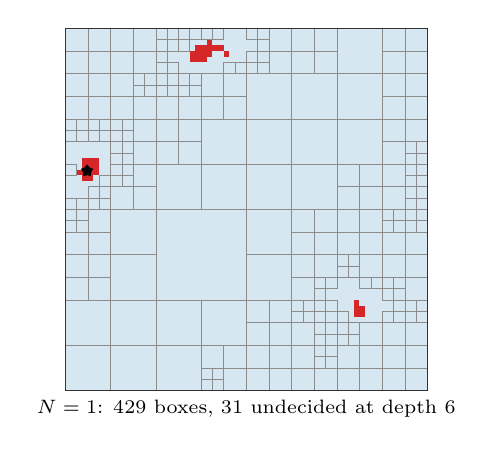
\begin{tikzpicture}[scale=4.6]
\fill[regA!18] (0.9375,0.9375) rectangle (1,1);
\fill[regA!18] (0.9375,0.875) rectangle (1,0.9375);
\fill[regA!18] (0.875,0.9375) rectangle (0.9375,1);
\fill[regA!18] (0.875,0.875) rectangle (0.9375,0.9375);
\fill[regA!18] (0.9375,0.8125) rectangle (1,0.875);
\fill[regA!18] (0.9375,0.75) rectangle (1,0.8125);
\fill[regA!18] (0.875,0.8125) rectangle (0.9375,0.875);
\fill[regA!18] (0.875,0.75) rectangle (0.9375,0.8125);
\fill[regA!18] (0.75,0.875) rectangle (0.875,1);
\fill[regA!18] (0.75,0.75) rectangle (0.875,0.875);
\fill[regA!18] (0.9375,0.6875) rectangle (1,0.75);
\fill[regA!18] (0.9688,0.6562) rectangle (1,0.6875);
\fill[regA!18] (0.9688,0.625) rectangle (1,0.6562);
\fill[regA!18] (0.9375,0.6562) rectangle (0.9688,0.6875);
\fill[regA!18] (0.9375,0.625) rectangle (0.9688,0.6562);
\fill[regA!18] (0.875,0.6875) rectangle (0.9375,0.75);
\fill[regA!18] (0.875,0.625) rectangle (0.9375,0.6875);
\fill[regA!18] (0.9844,0.6094) rectangle (1,0.625);
\fill[regA!18] (0.9844,0.5938) rectangle (1,0.6094);
\fill[regA!18] (0.9688,0.6094) rectangle (0.9844,0.625);
\fill[regA!18] (0.9688,0.5938) rectangle (0.9844,0.6094);
\fill[regA!18] (0.9688,0.5625) rectangle (1,0.5938);
\fill[regA!18] (0.9375,0.5938) rectangle (0.9688,0.625);
\fill[regA!18] (0.9375,0.5625) rectangle (0.9688,0.5938);
\fill[regA!18] (0.9688,0.5312) rectangle (1,0.5625);
\fill[regA!18] (0.9688,0.5) rectangle (1,0.5312);
\fill[regA!18] (0.9375,0.5312) rectangle (0.9688,0.5625);
\fill[regA!18] (0.9375,0.5) rectangle (0.9688,0.5312);
\fill[regA!18] (0.875,0.5625) rectangle (0.9375,0.625);
\fill[regA!18] (0.875,0.5) rectangle (0.9375,0.5625);
\fill[regA!18] (0.75,0.625) rectangle (0.875,0.75);
\fill[regA!18] (0.8125,0.5625) rectangle (0.875,0.625);
\fill[regA!18] (0.8125,0.5) rectangle (0.875,0.5625);
\fill[regA!18] (0.75,0.5625) rectangle (0.8125,0.625);
\fill[regA!18] (0.75,0.5) rectangle (0.8125,0.5625);
\fill[regA!18] (0.6875,0.9375) rectangle (0.75,1);
\fill[regA!18] (0.6875,0.875) rectangle (0.75,0.9375);
\fill[regA!18] (0.625,0.9375) rectangle (0.6875,1);
\fill[regA!18] (0.625,0.875) rectangle (0.6875,0.9375);
\fill[regA!18] (0.625,0.75) rectangle (0.75,0.875);
\fill[regA!18] (0.5625,0.9375) rectangle (0.625,1);
\fill[regA!18] (0.5625,0.875) rectangle (0.625,0.9375);
\fill[regA!18] (0.5312,0.9688) rectangle (0.5625,1);
\fill[regA!18] (0.5312,0.9375) rectangle (0.5625,0.9688);
\fill[regA!18] (0.5,0.9688) rectangle (0.5312,1);
\fill[regA!18] (0.5156,0.9531) rectangle (0.5312,0.9688);
\fill[regA!18] (0.5156,0.9375) rectangle (0.5312,0.9531);
\fill[regA!18] (0.5,0.9531) rectangle (0.5156,0.9688);
\fill[regA!18] (0.5,0.9375) rectangle (0.5156,0.9531);
\fill[regA!18] (0.5312,0.9062) rectangle (0.5625,0.9375);
\fill[regA!18] (0.5312,0.875) rectangle (0.5625,0.9062);
\fill[regA!18] (0.5,0.9062) rectangle (0.5312,0.9375);
\fill[regA!18] (0.5,0.875) rectangle (0.5312,0.9062);
\fill[regA!18] (0.5,0.75) rectangle (0.625,0.875);
\fill[regA!18] (0.625,0.625) rectangle (0.75,0.75);
\fill[regA!18] (0.625,0.5) rectangle (0.75,0.625);
\fill[regA!18] (0.5,0.625) rectangle (0.625,0.75);
\fill[regA!18] (0.5,0.5) rectangle (0.625,0.625);
\fill[regA!18] (0.9688,0.4688) rectangle (1,0.5);
\fill[regA!18] (0.9688,0.4375) rectangle (1,0.4688);
\fill[regA!18] (0.9375,0.4688) rectangle (0.9688,0.5);
\fill[regA!18] (0.9375,0.4375) rectangle (0.9688,0.4688);
\fill[regA!18] (0.9375,0.375) rectangle (1,0.4375);
\fill[regA!18] (0.9062,0.4688) rectangle (0.9375,0.5);
\fill[regA!18] (0.9062,0.4375) rectangle (0.9375,0.4688);
\fill[regA!18] (0.875,0.4688) rectangle (0.9062,0.5);
\fill[regA!18] (0.875,0.4375) rectangle (0.9062,0.4688);
\fill[regA!18] (0.875,0.375) rectangle (0.9375,0.4375);
\fill[regA!18] (0.9375,0.3125) rectangle (1,0.375);
\fill[regA!18] (0.9375,0.25) rectangle (1,0.3125);
\fill[regA!18] (0.875,0.3125) rectangle (0.9375,0.375);
\fill[regA!18] (0.9062,0.2812) rectangle (0.9375,0.3125);
\fill[regA!18] (0.9062,0.25) rectangle (0.9375,0.2812);
\fill[regA!18] (0.875,0.2812) rectangle (0.9062,0.3125);
\fill[regA!18] (0.875,0.25) rectangle (0.9062,0.2812);
\fill[regA!18] (0.8125,0.4375) rectangle (0.875,0.5);
\fill[regA!18] (0.8125,0.375) rectangle (0.875,0.4375);
\fill[regA!18] (0.75,0.4375) rectangle (0.8125,0.5);
\fill[regA!18] (0.75,0.375) rectangle (0.8125,0.4375);
\fill[regA!18] (0.8125,0.3125) rectangle (0.875,0.375);
\fill[regA!18] (0.8438,0.2812) rectangle (0.875,0.3125);
\fill[regA!18] (0.8594,0.2656) rectangle (0.875,0.2812);
\fill[regA!18] (0.8594,0.25) rectangle (0.875,0.2656);
\fill[regA!18] (0.8438,0.2656) rectangle (0.8594,0.2812);
\fill[regA!18] (0.8438,0.25) rectangle (0.8594,0.2656);
\fill[regA!18] (0.8125,0.2812) rectangle (0.8438,0.3125);
\fill[regA!18] (0.8281,0.2656) rectangle (0.8438,0.2812);
\fill[regA!18] (0.8281,0.25) rectangle (0.8438,0.2656);
\fill[regA!18] (0.8125,0.2656) rectangle (0.8281,0.2812);
\fill[regA!18] (0.8125,0.25) rectangle (0.8281,0.2656);
\fill[regA!18] (0.7812,0.3438) rectangle (0.8125,0.375);
\fill[regA!18] (0.7812,0.3125) rectangle (0.8125,0.3438);
\fill[regA!18] (0.75,0.3438) rectangle (0.7812,0.375);
\fill[regA!18] (0.75,0.3125) rectangle (0.7812,0.3438);
\fill[regA!18] (0.7969,0.2969) rectangle (0.8125,0.3125);
\fill[regA!18] (0.7969,0.2812) rectangle (0.8125,0.2969);
\fill[regA!18] (0.7812,0.2969) rectangle (0.7969,0.3125);
\fill[regA!18] (0.7812,0.2812) rectangle (0.7969,0.2969);
\fill[regA!18] (0.7969,0.2656) rectangle (0.8125,0.2812);
\fill[regA!18] (0.7969,0.25) rectangle (0.8125,0.2656);
\fill[regA!18] (0.7812,0.2656) rectangle (0.7969,0.2812);
\fill[regA!18] (0.7812,0.25) rectangle (0.7969,0.2656);
\fill[regA!18] (0.7656,0.2969) rectangle (0.7812,0.3125);
\fill[regA!18] (0.7656,0.2812) rectangle (0.7812,0.2969);
\fill[regA!18] (0.75,0.2969) rectangle (0.7656,0.3125);
\fill[regA!18] (0.75,0.2812) rectangle (0.7656,0.2969);
\fill[regA!18] (0.7656,0.2656) rectangle (0.7812,0.2812);
\fill[regA!18] (0.7656,0.25) rectangle (0.7812,0.2656);
\fill[regA!18] (0.75,0.2656) rectangle (0.7656,0.2812);
\fill[regA!18] (0.75,0.25) rectangle (0.7656,0.2656);
\fill[regA!18] (0.9688,0.2188) rectangle (1,0.25);
\fill[regA!18] (0.9688,0.1875) rectangle (1,0.2188);
\fill[regA!18] (0.9375,0.2188) rectangle (0.9688,0.25);
\fill[regA!18] (0.9375,0.1875) rectangle (0.9688,0.2188);
\fill[regA!18] (0.9375,0.125) rectangle (1,0.1875);
\fill[regA!18] (0.9062,0.2188) rectangle (0.9375,0.25);
\fill[regA!18] (0.9062,0.1875) rectangle (0.9375,0.2188);
\fill[regA!18] (0.8906,0.2344) rectangle (0.9062,0.25);
\fill[regA!18] (0.8906,0.2188) rectangle (0.9062,0.2344);
\fill[regA!18] (0.875,0.2344) rectangle (0.8906,0.25);
\fill[regA!18] (0.875,0.2188) rectangle (0.8906,0.2344);
\fill[regA!18] (0.875,0.1875) rectangle (0.9062,0.2188);
\fill[regA!18] (0.875,0.125) rectangle (0.9375,0.1875);
\fill[regA!18] (0.9375,0.0625) rectangle (1,0.125);
\fill[regA!18] (0.9375,0) rectangle (1,0.0625);
\fill[regA!18] (0.875,0.0625) rectangle (0.9375,0.125);
\fill[regA!18] (0.875,0) rectangle (0.9375,0.0625);
\fill[regA!18] (0.8594,0.2344) rectangle (0.875,0.25);
\fill[regA!18] (0.8594,0.2188) rectangle (0.875,0.2344);
\fill[regA!18] (0.8438,0.2344) rectangle (0.8594,0.25);
\fill[regA!18] (0.8438,0.2188) rectangle (0.8594,0.2344);
\fill[regA!18] (0.8594,0.2031) rectangle (0.875,0.2188);
\fill[regA!18] (0.8594,0.1875) rectangle (0.875,0.2031);
\fill[regA!18] (0.8438,0.2031) rectangle (0.8594,0.2188);
\fill[regA!18] (0.8438,0.1875) rectangle (0.8594,0.2031);
\fill[regA!18] (0.8281,0.2344) rectangle (0.8438,0.25);
\fill[regA!18] (0.8281,0.2188) rectangle (0.8438,0.2344);
\fill[regA!18] (0.8125,0.2344) rectangle (0.8281,0.25);
\fill[regA!18] (0.8281,0.2031) rectangle (0.8438,0.2188);
\fill[regA!18] (0.8281,0.1875) rectangle (0.8438,0.2031);
\fill[regA!18] (0.8125,0.1875) rectangle (0.8281,0.2031);
\fill[regA!18] (0.8125,0.125) rectangle (0.875,0.1875);
\fill[regA!18] (0.7812,0.2344) rectangle (0.7969,0.25);
\fill[regA!18] (0.7812,0.2188) rectangle (0.7969,0.2344);
\fill[regA!18] (0.7969,0.1875) rectangle (0.8125,0.2031);
\fill[regA!18] (0.7812,0.2031) rectangle (0.7969,0.2188);
\fill[regA!18] (0.7812,0.1875) rectangle (0.7969,0.2031);
\fill[regA!18] (0.7656,0.2344) rectangle (0.7812,0.25);
\fill[regA!18] (0.7656,0.2188) rectangle (0.7812,0.2344);
\fill[regA!18] (0.75,0.2344) rectangle (0.7656,0.25);
\fill[regA!18] (0.75,0.2188) rectangle (0.7656,0.2344);
\fill[regA!18] (0.75,0.1875) rectangle (0.7812,0.2188);
\fill[regA!18] (0.7812,0.1562) rectangle (0.8125,0.1875);
\fill[regA!18] (0.7812,0.125) rectangle (0.8125,0.1562);
\fill[regA!18] (0.75,0.1562) rectangle (0.7812,0.1875);
\fill[regA!18] (0.75,0.125) rectangle (0.7812,0.1562);
\fill[regA!18] (0.8125,0.0625) rectangle (0.875,0.125);
\fill[regA!18] (0.8125,0) rectangle (0.875,0.0625);
\fill[regA!18] (0.75,0.0625) rectangle (0.8125,0.125);
\fill[regA!18] (0.75,0) rectangle (0.8125,0.0625);
\fill[regA!18] (0.6875,0.4375) rectangle (0.75,0.5);
\fill[regA!18] (0.6875,0.375) rectangle (0.75,0.4375);
\fill[regA!18] (0.625,0.4375) rectangle (0.6875,0.5);
\fill[regA!18] (0.625,0.375) rectangle (0.6875,0.4375);
\fill[regA!18] (0.6875,0.3125) rectangle (0.75,0.375);
\fill[regA!18] (0.7188,0.2812) rectangle (0.75,0.3125);
\fill[regA!18] (0.7344,0.2656) rectangle (0.75,0.2812);
\fill[regA!18] (0.7344,0.25) rectangle (0.75,0.2656);
\fill[regA!18] (0.7188,0.2656) rectangle (0.7344,0.2812);
\fill[regA!18] (0.7188,0.25) rectangle (0.7344,0.2656);
\fill[regA!18] (0.6875,0.2812) rectangle (0.7188,0.3125);
\fill[regA!18] (0.6875,0.25) rectangle (0.7188,0.2812);
\fill[regA!18] (0.625,0.3125) rectangle (0.6875,0.375);
\fill[regA!18] (0.625,0.25) rectangle (0.6875,0.3125);
\fill[regA!18] (0.5,0.375) rectangle (0.625,0.5);
\fill[regA!18] (0.5,0.25) rectangle (0.625,0.375);
\fill[regA!18] (0.7188,0.2188) rectangle (0.75,0.25);
\fill[regA!18] (0.7188,0.1875) rectangle (0.75,0.2188);
\fill[regA!18] (0.6875,0.2188) rectangle (0.7188,0.25);
\fill[regA!18] (0.6875,0.1875) rectangle (0.7188,0.2188);
\fill[regA!18] (0.7188,0.1562) rectangle (0.75,0.1875);
\fill[regA!18] (0.7188,0.125) rectangle (0.75,0.1562);
\fill[regA!18] (0.6875,0.1562) rectangle (0.7188,0.1875);
\fill[regA!18] (0.6875,0.125) rectangle (0.7188,0.1562);
\fill[regA!18] (0.6562,0.2188) rectangle (0.6875,0.25);
\fill[regA!18] (0.6562,0.1875) rectangle (0.6875,0.2188);
\fill[regA!18] (0.625,0.2188) rectangle (0.6562,0.25);
\fill[regA!18] (0.625,0.1875) rectangle (0.6562,0.2188);
\fill[regA!18] (0.625,0.125) rectangle (0.6875,0.1875);
\fill[regA!18] (0.7188,0.0938) rectangle (0.75,0.125);
\fill[regA!18] (0.7188,0.0625) rectangle (0.75,0.0938);
\fill[regA!18] (0.6875,0.0938) rectangle (0.7188,0.125);
\fill[regA!18] (0.6875,0.0625) rectangle (0.7188,0.0938);
\fill[regA!18] (0.6875,0) rectangle (0.75,0.0625);
\fill[regA!18] (0.625,0.0625) rectangle (0.6875,0.125);
\fill[regA!18] (0.625,0) rectangle (0.6875,0.0625);
\fill[regA!18] (0.5625,0.1875) rectangle (0.625,0.25);
\fill[regA!18] (0.5625,0.125) rectangle (0.625,0.1875);
\fill[regA!18] (0.5,0.1875) rectangle (0.5625,0.25);
\fill[regA!18] (0.5,0.125) rectangle (0.5625,0.1875);
\fill[regA!18] (0.5625,0.0625) rectangle (0.625,0.125);
\fill[regA!18] (0.5625,0) rectangle (0.625,0.0625);
\fill[regA!18] (0.5,0.0625) rectangle (0.5625,0.125);
\fill[regA!18] (0.5,0) rectangle (0.5625,0.0625);
\fill[regA!18] (0.4844,0.9844) rectangle (0.5,1);
\fill[regA!18] (0.4844,0.9688) rectangle (0.5,0.9844);
\fill[regA!18] (0.4688,0.9844) rectangle (0.4844,1);
\fill[regA!18] (0.4688,0.9688) rectangle (0.4844,0.9844);
\fill[regA!18] (0.4844,0.9531) rectangle (0.5,0.9688);
\fill[regA!18] (0.4844,0.9375) rectangle (0.5,0.9531);
\fill[regA!18] (0.4688,0.9531) rectangle (0.4844,0.9688);
\fill[regA!18] (0.4688,0.9375) rectangle (0.4844,0.9531);
\fill[regA!18] (0.4531,0.9844) rectangle (0.4688,1);
\fill[regA!18] (0.4531,0.9688) rectangle (0.4688,0.9844);
\fill[regA!18] (0.4375,0.9844) rectangle (0.4531,1);
\fill[regA!18] (0.4375,0.9688) rectangle (0.4531,0.9844);
\fill[regA!18] (0.4531,0.9531) rectangle (0.4688,0.9688);
\fill[regA!18] (0.4531,0.9375) rectangle (0.4688,0.9531);
\fill[regA!18] (0.4375,0.9531) rectangle (0.4531,0.9688);
\fill[regA!18] (0.4375,0.9375) rectangle (0.4531,0.9531);
\fill[regA!18] (0.4844,0.9219) rectangle (0.5,0.9375);
\fill[regA!18] (0.4844,0.9062) rectangle (0.5,0.9219);
\fill[regA!18] (0.4688,0.9219) rectangle (0.4844,0.9375);
\fill[regA!18] (0.4688,0.9062) rectangle (0.4844,0.9219);
\fill[regA!18] (0.4688,0.875) rectangle (0.5,0.9062);
\fill[regA!18] (0.4531,0.9219) rectangle (0.4688,0.9375);
\fill[regA!18] (0.4531,0.9062) rectangle (0.4688,0.9219);
\fill[regA!18] (0.4375,0.9062) rectangle (0.4531,0.9219);
\fill[regA!18] (0.4375,0.875) rectangle (0.4688,0.9062);
\fill[regA!18] (0.4062,0.9688) rectangle (0.4375,1);
\fill[regA!18] (0.4219,0.9531) rectangle (0.4375,0.9688);
\fill[regA!18] (0.4062,0.9531) rectangle (0.4219,0.9688);
\fill[regA!18] (0.375,0.9688) rectangle (0.4062,1);
\fill[regA!18] (0.375,0.9531) rectangle (0.3906,0.9688);
\fill[regA!18] (0.4219,0.9219) rectangle (0.4375,0.9375);
\fill[regA!18] (0.4219,0.9062) rectangle (0.4375,0.9219);
\fill[regA!18] (0.4062,0.9219) rectangle (0.4219,0.9375);
\fill[regA!18] (0.4062,0.9062) rectangle (0.4219,0.9219);
\fill[regA!18] (0.4219,0.8906) rectangle (0.4375,0.9062);
\fill[regA!18] (0.4219,0.875) rectangle (0.4375,0.8906);
\fill[regA!18] (0.4062,0.8906) rectangle (0.4219,0.9062);
\fill[regA!18] (0.4062,0.875) rectangle (0.4219,0.8906);
\fill[regA!18] (0.3906,0.9062) rectangle (0.4062,0.9219);
\fill[regA!18] (0.3906,0.8906) rectangle (0.4062,0.9062);
\fill[regA!18] (0.3906,0.875) rectangle (0.4062,0.8906);
\fill[regA!18] (0.375,0.8906) rectangle (0.3906,0.9062);
\fill[regA!18] (0.375,0.875) rectangle (0.3906,0.8906);
\fill[regA!18] (0.4375,0.8125) rectangle (0.5,0.875);
\fill[regA!18] (0.4375,0.75) rectangle (0.5,0.8125);
\fill[regA!18] (0.375,0.8125) rectangle (0.4375,0.875);
\fill[regA!18] (0.375,0.75) rectangle (0.4375,0.8125);
\fill[regA!18] (0.3438,0.9688) rectangle (0.375,1);
\fill[regA!18] (0.3594,0.9531) rectangle (0.375,0.9688);
\fill[regA!18] (0.3438,0.9531) rectangle (0.3594,0.9688);
\fill[regA!18] (0.3438,0.9375) rectangle (0.3594,0.9531);
\fill[regA!18] (0.3125,0.9688) rectangle (0.3438,1);
\fill[regA!18] (0.3125,0.9375) rectangle (0.3438,0.9688);
\fill[regA!18] (0.3594,0.8906) rectangle (0.375,0.9062);
\fill[regA!18] (0.3594,0.875) rectangle (0.375,0.8906);
\fill[regA!18] (0.3438,0.8906) rectangle (0.3594,0.9062);
\fill[regA!18] (0.3438,0.875) rectangle (0.3594,0.8906);
\fill[regA!18] (0.3281,0.9219) rectangle (0.3438,0.9375);
\fill[regA!18] (0.3281,0.9062) rectangle (0.3438,0.9219);
\fill[regA!18] (0.3125,0.9219) rectangle (0.3281,0.9375);
\fill[regA!18] (0.3125,0.9062) rectangle (0.3281,0.9219);
\fill[regA!18] (0.3281,0.8906) rectangle (0.3438,0.9062);
\fill[regA!18] (0.3281,0.875) rectangle (0.3438,0.8906);
\fill[regA!18] (0.3125,0.8906) rectangle (0.3281,0.9062);
\fill[regA!18] (0.3125,0.875) rectangle (0.3281,0.8906);
\fill[regA!18] (0.2812,0.9688) rectangle (0.3125,1);
\fill[regA!18] (0.2812,0.9375) rectangle (0.3125,0.9688);
\fill[regA!18] (0.25,0.9688) rectangle (0.2812,1);
\fill[regA!18] (0.25,0.9375) rectangle (0.2812,0.9688);
\fill[regA!18] (0.2969,0.9219) rectangle (0.3125,0.9375);
\fill[regA!18] (0.2969,0.9062) rectangle (0.3125,0.9219);
\fill[regA!18] (0.2812,0.9219) rectangle (0.2969,0.9375);
\fill[regA!18] (0.2812,0.9062) rectangle (0.2969,0.9219);
\fill[regA!18] (0.2812,0.875) rectangle (0.3125,0.9062);
\fill[regA!18] (0.25,0.9062) rectangle (0.2812,0.9375);
\fill[regA!18] (0.25,0.875) rectangle (0.2812,0.9062);
\fill[regA!18] (0.3438,0.8438) rectangle (0.375,0.875);
\fill[regA!18] (0.3438,0.8125) rectangle (0.375,0.8438);
\fill[regA!18] (0.3125,0.8438) rectangle (0.3438,0.875);
\fill[regA!18] (0.3125,0.8125) rectangle (0.3438,0.8438);
\fill[regA!18] (0.3125,0.75) rectangle (0.375,0.8125);
\fill[regA!18] (0.2812,0.8438) rectangle (0.3125,0.875);
\fill[regA!18] (0.2812,0.8125) rectangle (0.3125,0.8438);
\fill[regA!18] (0.25,0.8438) rectangle (0.2812,0.875);
\fill[regA!18] (0.25,0.8125) rectangle (0.2812,0.8438);
\fill[regA!18] (0.25,0.75) rectangle (0.3125,0.8125);
\fill[regA!18] (0.375,0.625) rectangle (0.5,0.75);
\fill[regA!18] (0.375,0.5) rectangle (0.5,0.625);
\fill[regA!18] (0.3125,0.6875) rectangle (0.375,0.75);
\fill[regA!18] (0.3125,0.625) rectangle (0.375,0.6875);
\fill[regA!18] (0.25,0.6875) rectangle (0.3125,0.75);
\fill[regA!18] (0.25,0.625) rectangle (0.3125,0.6875);
\fill[regA!18] (0.25,0.5) rectangle (0.375,0.625);
\fill[regA!18] (0.1875,0.9375) rectangle (0.25,1);
\fill[regA!18] (0.1875,0.875) rectangle (0.25,0.9375);
\fill[regA!18] (0.125,0.9375) rectangle (0.1875,1);
\fill[regA!18] (0.125,0.875) rectangle (0.1875,0.9375);
\fill[regA!18] (0.2188,0.8438) rectangle (0.25,0.875);
\fill[regA!18] (0.2188,0.8125) rectangle (0.25,0.8438);
\fill[regA!18] (0.1875,0.8438) rectangle (0.2188,0.875);
\fill[regA!18] (0.1875,0.8125) rectangle (0.2188,0.8438);
\fill[regA!18] (0.1875,0.75) rectangle (0.25,0.8125);
\fill[regA!18] (0.125,0.8125) rectangle (0.1875,0.875);
\fill[regA!18] (0.125,0.75) rectangle (0.1875,0.8125);
\fill[regA!18] (0.0625,0.9375) rectangle (0.125,1);
\fill[regA!18] (0.0625,0.875) rectangle (0.125,0.9375);
\fill[regA!18] (0,0.9375) rectangle (0.0625,1);
\fill[regA!18] (0,0.875) rectangle (0.0625,0.9375);
\fill[regA!18] (0.0625,0.8125) rectangle (0.125,0.875);
\fill[regA!18] (0.0625,0.75) rectangle (0.125,0.8125);
\fill[regA!18] (0,0.8125) rectangle (0.0625,0.875);
\fill[regA!18] (0,0.75) rectangle (0.0625,0.8125);
\fill[regA!18] (0.1875,0.6875) rectangle (0.25,0.75);
\fill[regA!18] (0.1875,0.625) rectangle (0.25,0.6875);
\fill[regA!18] (0.1562,0.7188) rectangle (0.1875,0.75);
\fill[regA!18] (0.1562,0.6875) rectangle (0.1875,0.7188);
\fill[regA!18] (0.125,0.7188) rectangle (0.1562,0.75);
\fill[regA!18] (0.125,0.6875) rectangle (0.1562,0.7188);
\fill[regA!18] (0.1562,0.6562) rectangle (0.1875,0.6875);
\fill[regA!18] (0.1562,0.625) rectangle (0.1875,0.6562);
\fill[regA!18] (0.125,0.6562) rectangle (0.1562,0.6875);
\fill[regA!18] (0.125,0.625) rectangle (0.1562,0.6562);
\fill[regA!18] (0.1875,0.5625) rectangle (0.25,0.625);
\fill[regA!18] (0.1875,0.5) rectangle (0.25,0.5625);
\fill[regA!18] (0.1562,0.5938) rectangle (0.1875,0.625);
\fill[regA!18] (0.1562,0.5625) rectangle (0.1875,0.5938);
\fill[regA!18] (0.125,0.5938) rectangle (0.1562,0.625);
\fill[regA!18] (0.125,0.5625) rectangle (0.1562,0.5938);
\fill[regA!18] (0.125,0.5) rectangle (0.1875,0.5625);
\fill[regA!18] (0.0938,0.7188) rectangle (0.125,0.75);
\fill[regA!18] (0.0938,0.6875) rectangle (0.125,0.7188);
\fill[regA!18] (0.0625,0.7188) rectangle (0.0938,0.75);
\fill[regA!18] (0.0625,0.6875) rectangle (0.0938,0.7188);
\fill[regA!18] (0.1094,0.6719) rectangle (0.125,0.6875);
\fill[regA!18] (0.1094,0.6562) rectangle (0.125,0.6719);
\fill[regA!18] (0.0938,0.6719) rectangle (0.1094,0.6875);
\fill[regA!18] (0.0938,0.6562) rectangle (0.1094,0.6719);
\fill[regA!18] (0.1094,0.6406) rectangle (0.125,0.6562);
\fill[regA!18] (0.1094,0.625) rectangle (0.125,0.6406);
\fill[regA!18] (0.0938,0.6406) rectangle (0.1094,0.6562);
\fill[regA!18] (0.0938,0.625) rectangle (0.1094,0.6406);
\fill[regA!18] (0.0781,0.6719) rectangle (0.0938,0.6875);
\fill[regA!18] (0.0781,0.6562) rectangle (0.0938,0.6719);
\fill[regA!18] (0.0625,0.6719) rectangle (0.0781,0.6875);
\fill[regA!18] (0.0625,0.6562) rectangle (0.0781,0.6719);
\fill[regA!18] (0.0781,0.6406) rectangle (0.0938,0.6562);
\fill[regA!18] (0.0625,0.6406) rectangle (0.0781,0.6562);
\fill[regA!18] (0.0312,0.7188) rectangle (0.0625,0.75);
\fill[regA!18] (0.0312,0.6875) rectangle (0.0625,0.7188);
\fill[regA!18] (0,0.7188) rectangle (0.0312,0.75);
\fill[regA!18] (0,0.6875) rectangle (0.0312,0.7188);
\fill[regA!18] (0.0469,0.6719) rectangle (0.0625,0.6875);
\fill[regA!18] (0.0469,0.6562) rectangle (0.0625,0.6719);
\fill[regA!18] (0.0312,0.6719) rectangle (0.0469,0.6875);
\fill[regA!18] (0.0312,0.6562) rectangle (0.0469,0.6719);
\fill[regA!18] (0.0469,0.6406) rectangle (0.0625,0.6562);
\fill[regA!18] (0.0312,0.6406) rectangle (0.0469,0.6562);
\fill[regA!18] (0.0312,0.625) rectangle (0.0469,0.6406);
\fill[regA!18] (0.0156,0.6719) rectangle (0.0312,0.6875);
\fill[regA!18] (0.0156,0.6562) rectangle (0.0312,0.6719);
\fill[regA!18] (0,0.6719) rectangle (0.0156,0.6875);
\fill[regA!18] (0,0.6562) rectangle (0.0156,0.6719);
\fill[regA!18] (0.0156,0.6406) rectangle (0.0312,0.6562);
\fill[regA!18] (0.0156,0.625) rectangle (0.0312,0.6406);
\fill[regA!18] (0,0.6406) rectangle (0.0156,0.6562);
\fill[regA!18] (0,0.625) rectangle (0.0156,0.6406);
\fill[regA!18] (0.1094,0.6094) rectangle (0.125,0.625);
\fill[regA!18] (0.1094,0.5938) rectangle (0.125,0.6094);
\fill[regA!18] (0.0938,0.6094) rectangle (0.1094,0.625);
\fill[regA!18] (0.0938,0.5938) rectangle (0.1094,0.6094);
\fill[regA!18] (0.0938,0.5625) rectangle (0.125,0.5938);
\fill[regA!18] (0.0781,0.5781) rectangle (0.0938,0.5938);
\fill[regA!18] (0.0781,0.5625) rectangle (0.0938,0.5781);
\fill[regA!18] (0.0625,0.5625) rectangle (0.0781,0.5781);
\fill[regA!18] (0.0938,0.5312) rectangle (0.125,0.5625);
\fill[regA!18] (0.0938,0.5) rectangle (0.125,0.5312);
\fill[regA!18] (0.0625,0.5312) rectangle (0.0938,0.5625);
\fill[regA!18] (0.0625,0.5) rectangle (0.0938,0.5312);
\fill[regA!18] (0.0312,0.6094) rectangle (0.0469,0.625);
\fill[regA!18] (0.0469,0.5625) rectangle (0.0625,0.5781);
\fill[regA!18] (0.0312,0.5781) rectangle (0.0469,0.5938);
\fill[regA!18] (0.0312,0.5625) rectangle (0.0469,0.5781);
\fill[regA!18] (0,0.5938) rectangle (0.0312,0.625);
\fill[regA!18] (0.0156,0.5781) rectangle (0.0312,0.5938);
\fill[regA!18] (0.0156,0.5625) rectangle (0.0312,0.5781);
\fill[regA!18] (0,0.5781) rectangle (0.0156,0.5938);
\fill[regA!18] (0,0.5625) rectangle (0.0156,0.5781);
\fill[regA!18] (0.0469,0.5469) rectangle (0.0625,0.5625);
\fill[regA!18] (0.0469,0.5312) rectangle (0.0625,0.5469);
\fill[regA!18] (0.0312,0.5469) rectangle (0.0469,0.5625);
\fill[regA!18] (0.0312,0.5312) rectangle (0.0469,0.5469);
\fill[regA!18] (0.0312,0.5) rectangle (0.0625,0.5312);
\fill[regA!18] (0.0156,0.5469) rectangle (0.0312,0.5625);
\fill[regA!18] (0.0156,0.5312) rectangle (0.0312,0.5469);
\fill[regA!18] (0,0.5469) rectangle (0.0156,0.5625);
\fill[regA!18] (0,0.5312) rectangle (0.0156,0.5469);
\fill[regA!18] (0,0.5) rectangle (0.0312,0.5312);
\fill[regA!18] (0.25,0.25) rectangle (0.5,0.5);
\fill[regA!18] (0.375,0.125) rectangle (0.5,0.25);
\fill[regA!18] (0.4375,0.0625) rectangle (0.5,0.125);
\fill[regA!18] (0.4375,0) rectangle (0.5,0.0625);
\fill[regA!18] (0.375,0.0625) rectangle (0.4375,0.125);
\fill[regA!18] (0.4062,0.0312) rectangle (0.4375,0.0625);
\fill[regA!18] (0.4062,0) rectangle (0.4375,0.0312);
\fill[regA!18] (0.375,0.0312) rectangle (0.4062,0.0625);
\fill[regA!18] (0.375,0) rectangle (0.4062,0.0312);
\fill[regA!18] (0.25,0.125) rectangle (0.375,0.25);
\fill[regA!18] (0.25,0) rectangle (0.375,0.125);
\fill[regA!18] (0.125,0.375) rectangle (0.25,0.5);
\fill[regA!18] (0.125,0.25) rectangle (0.25,0.375);
\fill[regA!18] (0.0625,0.4375) rectangle (0.125,0.5);
\fill[regA!18] (0.0625,0.375) rectangle (0.125,0.4375);
\fill[regA!18] (0.0312,0.4688) rectangle (0.0625,0.5);
\fill[regA!18] (0.0312,0.4375) rectangle (0.0625,0.4688);
\fill[regA!18] (0,0.4688) rectangle (0.0312,0.5);
\fill[regA!18] (0,0.4375) rectangle (0.0312,0.4688);
\fill[regA!18] (0,0.375) rectangle (0.0625,0.4375);
\fill[regA!18] (0.0625,0.3125) rectangle (0.125,0.375);
\fill[regA!18] (0.0625,0.25) rectangle (0.125,0.3125);
\fill[regA!18] (0,0.3125) rectangle (0.0625,0.375);
\fill[regA!18] (0,0.25) rectangle (0.0625,0.3125);
\fill[regA!18] (0.125,0.125) rectangle (0.25,0.25);
\fill[regA!18] (0.125,0) rectangle (0.25,0.125);
\fill[regA!18] (0,0.125) rectangle (0.125,0.25);
\fill[regA!18] (0,0) rectangle (0.125,0.125);
\fill[bad] (0.8125,0.2188) rectangle (0.8281,0.2344);
\fill[bad] (0.8125,0.2031) rectangle (0.8281,0.2188);
\fill[bad] (0.7969,0.2344) rectangle (0.8125,0.25);
\fill[bad] (0.7969,0.2188) rectangle (0.8125,0.2344);
\fill[bad] (0.7969,0.2031) rectangle (0.8125,0.2188);
\fill[bad] (0.4375,0.9219) rectangle (0.4531,0.9375);
\fill[bad] (0.4219,0.9375) rectangle (0.4375,0.9531);
\fill[bad] (0.4062,0.9375) rectangle (0.4219,0.9531);
\fill[bad] (0.3906,0.9531) rectangle (0.4062,0.9688);
\fill[bad] (0.3906,0.9375) rectangle (0.4062,0.9531);
\fill[bad] (0.375,0.9375) rectangle (0.3906,0.9531);
\fill[bad] (0.3906,0.9219) rectangle (0.4062,0.9375);
\fill[bad] (0.375,0.9219) rectangle (0.3906,0.9375);
\fill[bad] (0.375,0.9062) rectangle (0.3906,0.9219);
\fill[bad] (0.3594,0.9375) rectangle (0.375,0.9531);
\fill[bad] (0.3594,0.9219) rectangle (0.375,0.9375);
\fill[bad] (0.3594,0.9062) rectangle (0.375,0.9219);
\fill[bad] (0.3438,0.9219) rectangle (0.3594,0.9375);
\fill[bad] (0.3438,0.9062) rectangle (0.3594,0.9219);
\fill[bad] (0.0781,0.625) rectangle (0.0938,0.6406);
\fill[bad] (0.0625,0.625) rectangle (0.0781,0.6406);
\fill[bad] (0.0469,0.625) rectangle (0.0625,0.6406);
\fill[bad] (0.0781,0.6094) rectangle (0.0938,0.625);
\fill[bad] (0.0781,0.5938) rectangle (0.0938,0.6094);
\fill[bad] (0.0625,0.6094) rectangle (0.0781,0.625);
\fill[bad] (0.0625,0.5938) rectangle (0.0781,0.6094);
\fill[bad] (0.0625,0.5781) rectangle (0.0781,0.5938);
\fill[bad] (0.0469,0.6094) rectangle (0.0625,0.625);
\fill[bad] (0.0469,0.5938) rectangle (0.0625,0.6094);
\fill[bad] (0.0312,0.5938) rectangle (0.0469,0.6094);
\fill[bad] (0.0469,0.5781) rectangle (0.0625,0.5938);
\draw[black!45, line width=0.15pt] (0.9375,0.9375) rectangle (1,1);
\draw[black!45, line width=0.15pt] (0.9375,0.875) rectangle (1,0.9375);
\draw[black!45, line width=0.15pt] (0.875,0.9375) rectangle (0.9375,1);
\draw[black!45, line width=0.15pt] (0.875,0.875) rectangle (0.9375,0.9375);
\draw[black!45, line width=0.15pt] (0.9375,0.8125) rectangle (1,0.875);
\draw[black!45, line width=0.15pt] (0.9375,0.75) rectangle (1,0.8125);
\draw[black!45, line width=0.15pt] (0.875,0.8125) rectangle (0.9375,0.875);
\draw[black!45, line width=0.15pt] (0.875,0.75) rectangle (0.9375,0.8125);
\draw[black!45, line width=0.15pt] (0.75,0.875) rectangle (0.875,1);
\draw[black!45, line width=0.15pt] (0.75,0.75) rectangle (0.875,0.875);
\draw[black!45, line width=0.15pt] (0.9375,0.6875) rectangle (1,0.75);
\draw[black!45, line width=0.15pt] (0.9688,0.6562) rectangle (1,0.6875);
\draw[black!45, line width=0.15pt] (0.9688,0.625) rectangle (1,0.6562);
\draw[black!45, line width=0.15pt] (0.9375,0.6562) rectangle (0.9688,0.6875);
\draw[black!45, line width=0.15pt] (0.9375,0.625) rectangle (0.9688,0.6562);
\draw[black!45, line width=0.15pt] (0.875,0.6875) rectangle (0.9375,0.75);
\draw[black!45, line width=0.15pt] (0.875,0.625) rectangle (0.9375,0.6875);
\draw[black!45, line width=0.15pt] (0.9688,0.5625) rectangle (1,0.5938);
\draw[black!45, line width=0.15pt] (0.9375,0.5938) rectangle (0.9688,0.625);
\draw[black!45, line width=0.15pt] (0.9375,0.5625) rectangle (0.9688,0.5938);
\draw[black!45, line width=0.15pt] (0.9688,0.5312) rectangle (1,0.5625);
\draw[black!45, line width=0.15pt] (0.9688,0.5) rectangle (1,0.5312);
\draw[black!45, line width=0.15pt] (0.9375,0.5312) rectangle (0.9688,0.5625);
\draw[black!45, line width=0.15pt] (0.9375,0.5) rectangle (0.9688,0.5312);
\draw[black!45, line width=0.15pt] (0.875,0.5625) rectangle (0.9375,0.625);
\draw[black!45, line width=0.15pt] (0.875,0.5) rectangle (0.9375,0.5625);
\draw[black!45, line width=0.15pt] (0.75,0.625) rectangle (0.875,0.75);
\draw[black!45, line width=0.15pt] (0.8125,0.5625) rectangle (0.875,0.625);
\draw[black!45, line width=0.15pt] (0.8125,0.5) rectangle (0.875,0.5625);
\draw[black!45, line width=0.15pt] (0.75,0.5625) rectangle (0.8125,0.625);
\draw[black!45, line width=0.15pt] (0.75,0.5) rectangle (0.8125,0.5625);
\draw[black!45, line width=0.15pt] (0.6875,0.9375) rectangle (0.75,1);
\draw[black!45, line width=0.15pt] (0.6875,0.875) rectangle (0.75,0.9375);
\draw[black!45, line width=0.15pt] (0.625,0.9375) rectangle (0.6875,1);
\draw[black!45, line width=0.15pt] (0.625,0.875) rectangle (0.6875,0.9375);
\draw[black!45, line width=0.15pt] (0.625,0.75) rectangle (0.75,0.875);
\draw[black!45, line width=0.15pt] (0.5625,0.9375) rectangle (0.625,1);
\draw[black!45, line width=0.15pt] (0.5625,0.875) rectangle (0.625,0.9375);
\draw[black!45, line width=0.15pt] (0.5312,0.9688) rectangle (0.5625,1);
\draw[black!45, line width=0.15pt] (0.5312,0.9375) rectangle (0.5625,0.9688);
\draw[black!45, line width=0.15pt] (0.5,0.9688) rectangle (0.5312,1);
\draw[black!45, line width=0.15pt] (0.5312,0.9062) rectangle (0.5625,0.9375);
\draw[black!45, line width=0.15pt] (0.5312,0.875) rectangle (0.5625,0.9062);
\draw[black!45, line width=0.15pt] (0.5,0.9062) rectangle (0.5312,0.9375);
\draw[black!45, line width=0.15pt] (0.5,0.875) rectangle (0.5312,0.9062);
\draw[black!45, line width=0.15pt] (0.5,0.75) rectangle (0.625,0.875);
\draw[black!45, line width=0.15pt] (0.625,0.625) rectangle (0.75,0.75);
\draw[black!45, line width=0.15pt] (0.625,0.5) rectangle (0.75,0.625);
\draw[black!45, line width=0.15pt] (0.5,0.625) rectangle (0.625,0.75);
\draw[black!45, line width=0.15pt] (0.5,0.5) rectangle (0.625,0.625);
\draw[black!45, line width=0.15pt] (0.9688,0.4688) rectangle (1,0.5);
\draw[black!45, line width=0.15pt] (0.9688,0.4375) rectangle (1,0.4688);
\draw[black!45, line width=0.15pt] (0.9375,0.4688) rectangle (0.9688,0.5);
\draw[black!45, line width=0.15pt] (0.9375,0.4375) rectangle (0.9688,0.4688);
\draw[black!45, line width=0.15pt] (0.9375,0.375) rectangle (1,0.4375);
\draw[black!45, line width=0.15pt] (0.9062,0.4688) rectangle (0.9375,0.5);
\draw[black!45, line width=0.15pt] (0.9062,0.4375) rectangle (0.9375,0.4688);
\draw[black!45, line width=0.15pt] (0.875,0.4688) rectangle (0.9062,0.5);
\draw[black!45, line width=0.15pt] (0.875,0.4375) rectangle (0.9062,0.4688);
\draw[black!45, line width=0.15pt] (0.875,0.375) rectangle (0.9375,0.4375);
\draw[black!45, line width=0.15pt] (0.9375,0.3125) rectangle (1,0.375);
\draw[black!45, line width=0.15pt] (0.9375,0.25) rectangle (1,0.3125);
\draw[black!45, line width=0.15pt] (0.875,0.3125) rectangle (0.9375,0.375);
\draw[black!45, line width=0.15pt] (0.9062,0.2812) rectangle (0.9375,0.3125);
\draw[black!45, line width=0.15pt] (0.9062,0.25) rectangle (0.9375,0.2812);
\draw[black!45, line width=0.15pt] (0.875,0.2812) rectangle (0.9062,0.3125);
\draw[black!45, line width=0.15pt] (0.875,0.25) rectangle (0.9062,0.2812);
\draw[black!45, line width=0.15pt] (0.8125,0.4375) rectangle (0.875,0.5);
\draw[black!45, line width=0.15pt] (0.8125,0.375) rectangle (0.875,0.4375);
\draw[black!45, line width=0.15pt] (0.75,0.4375) rectangle (0.8125,0.5);
\draw[black!45, line width=0.15pt] (0.75,0.375) rectangle (0.8125,0.4375);
\draw[black!45, line width=0.15pt] (0.8125,0.3125) rectangle (0.875,0.375);
\draw[black!45, line width=0.15pt] (0.8438,0.2812) rectangle (0.875,0.3125);
\draw[black!45, line width=0.15pt] (0.8125,0.2812) rectangle (0.8438,0.3125);
\draw[black!45, line width=0.15pt] (0.7812,0.3438) rectangle (0.8125,0.375);
\draw[black!45, line width=0.15pt] (0.7812,0.3125) rectangle (0.8125,0.3438);
\draw[black!45, line width=0.15pt] (0.75,0.3438) rectangle (0.7812,0.375);
\draw[black!45, line width=0.15pt] (0.75,0.3125) rectangle (0.7812,0.3438);
\draw[black!45, line width=0.15pt] (0.9688,0.2188) rectangle (1,0.25);
\draw[black!45, line width=0.15pt] (0.9688,0.1875) rectangle (1,0.2188);
\draw[black!45, line width=0.15pt] (0.9375,0.2188) rectangle (0.9688,0.25);
\draw[black!45, line width=0.15pt] (0.9375,0.1875) rectangle (0.9688,0.2188);
\draw[black!45, line width=0.15pt] (0.9375,0.125) rectangle (1,0.1875);
\draw[black!45, line width=0.15pt] (0.9062,0.2188) rectangle (0.9375,0.25);
\draw[black!45, line width=0.15pt] (0.9062,0.1875) rectangle (0.9375,0.2188);
\draw[black!45, line width=0.15pt] (0.875,0.1875) rectangle (0.9062,0.2188);
\draw[black!45, line width=0.15pt] (0.875,0.125) rectangle (0.9375,0.1875);
\draw[black!45, line width=0.15pt] (0.9375,0.0625) rectangle (1,0.125);
\draw[black!45, line width=0.15pt] (0.9375,0) rectangle (1,0.0625);
\draw[black!45, line width=0.15pt] (0.875,0.0625) rectangle (0.9375,0.125);
\draw[black!45, line width=0.15pt] (0.875,0) rectangle (0.9375,0.0625);
\draw[black!45, line width=0.15pt] (0.8125,0.125) rectangle (0.875,0.1875);
\draw[black!45, line width=0.15pt] (0.75,0.1875) rectangle (0.7812,0.2188);
\draw[black!45, line width=0.15pt] (0.7812,0.1562) rectangle (0.8125,0.1875);
\draw[black!45, line width=0.15pt] (0.7812,0.125) rectangle (0.8125,0.1562);
\draw[black!45, line width=0.15pt] (0.75,0.1562) rectangle (0.7812,0.1875);
\draw[black!45, line width=0.15pt] (0.75,0.125) rectangle (0.7812,0.1562);
\draw[black!45, line width=0.15pt] (0.8125,0.0625) rectangle (0.875,0.125);
\draw[black!45, line width=0.15pt] (0.8125,0) rectangle (0.875,0.0625);
\draw[black!45, line width=0.15pt] (0.75,0.0625) rectangle (0.8125,0.125);
\draw[black!45, line width=0.15pt] (0.75,0) rectangle (0.8125,0.0625);
\draw[black!45, line width=0.15pt] (0.6875,0.4375) rectangle (0.75,0.5);
\draw[black!45, line width=0.15pt] (0.6875,0.375) rectangle (0.75,0.4375);
\draw[black!45, line width=0.15pt] (0.625,0.4375) rectangle (0.6875,0.5);
\draw[black!45, line width=0.15pt] (0.625,0.375) rectangle (0.6875,0.4375);
\draw[black!45, line width=0.15pt] (0.6875,0.3125) rectangle (0.75,0.375);
\draw[black!45, line width=0.15pt] (0.7188,0.2812) rectangle (0.75,0.3125);
\draw[black!45, line width=0.15pt] (0.6875,0.2812) rectangle (0.7188,0.3125);
\draw[black!45, line width=0.15pt] (0.6875,0.25) rectangle (0.7188,0.2812);
\draw[black!45, line width=0.15pt] (0.625,0.3125) rectangle (0.6875,0.375);
\draw[black!45, line width=0.15pt] (0.625,0.25) rectangle (0.6875,0.3125);
\draw[black!45, line width=0.15pt] (0.5,0.375) rectangle (0.625,0.5);
\draw[black!45, line width=0.15pt] (0.5,0.25) rectangle (0.625,0.375);
\draw[black!45, line width=0.15pt] (0.7188,0.2188) rectangle (0.75,0.25);
\draw[black!45, line width=0.15pt] (0.7188,0.1875) rectangle (0.75,0.2188);
\draw[black!45, line width=0.15pt] (0.6875,0.2188) rectangle (0.7188,0.25);
\draw[black!45, line width=0.15pt] (0.6875,0.1875) rectangle (0.7188,0.2188);
\draw[black!45, line width=0.15pt] (0.7188,0.1562) rectangle (0.75,0.1875);
\draw[black!45, line width=0.15pt] (0.7188,0.125) rectangle (0.75,0.1562);
\draw[black!45, line width=0.15pt] (0.6875,0.1562) rectangle (0.7188,0.1875);
\draw[black!45, line width=0.15pt] (0.6875,0.125) rectangle (0.7188,0.1562);
\draw[black!45, line width=0.15pt] (0.6562,0.2188) rectangle (0.6875,0.25);
\draw[black!45, line width=0.15pt] (0.6562,0.1875) rectangle (0.6875,0.2188);
\draw[black!45, line width=0.15pt] (0.625,0.2188) rectangle (0.6562,0.25);
\draw[black!45, line width=0.15pt] (0.625,0.1875) rectangle (0.6562,0.2188);
\draw[black!45, line width=0.15pt] (0.625,0.125) rectangle (0.6875,0.1875);
\draw[black!45, line width=0.15pt] (0.7188,0.0938) rectangle (0.75,0.125);
\draw[black!45, line width=0.15pt] (0.7188,0.0625) rectangle (0.75,0.0938);
\draw[black!45, line width=0.15pt] (0.6875,0.0938) rectangle (0.7188,0.125);
\draw[black!45, line width=0.15pt] (0.6875,0.0625) rectangle (0.7188,0.0938);
\draw[black!45, line width=0.15pt] (0.6875,0) rectangle (0.75,0.0625);
\draw[black!45, line width=0.15pt] (0.625,0.0625) rectangle (0.6875,0.125);
\draw[black!45, line width=0.15pt] (0.625,0) rectangle (0.6875,0.0625);
\draw[black!45, line width=0.15pt] (0.5625,0.1875) rectangle (0.625,0.25);
\draw[black!45, line width=0.15pt] (0.5625,0.125) rectangle (0.625,0.1875);
\draw[black!45, line width=0.15pt] (0.5,0.1875) rectangle (0.5625,0.25);
\draw[black!45, line width=0.15pt] (0.5,0.125) rectangle (0.5625,0.1875);
\draw[black!45, line width=0.15pt] (0.5625,0.0625) rectangle (0.625,0.125);
\draw[black!45, line width=0.15pt] (0.5625,0) rectangle (0.625,0.0625);
\draw[black!45, line width=0.15pt] (0.5,0.0625) rectangle (0.5625,0.125);
\draw[black!45, line width=0.15pt] (0.5,0) rectangle (0.5625,0.0625);
\draw[black!45, line width=0.15pt] (0.4688,0.875) rectangle (0.5,0.9062);
\draw[black!45, line width=0.15pt] (0.4375,0.875) rectangle (0.4688,0.9062);
\draw[black!45, line width=0.15pt] (0.4062,0.9688) rectangle (0.4375,1);
\draw[black!45, line width=0.15pt] (0.375,0.9688) rectangle (0.4062,1);
\draw[black!45, line width=0.15pt] (0.4375,0.8125) rectangle (0.5,0.875);
\draw[black!45, line width=0.15pt] (0.4375,0.75) rectangle (0.5,0.8125);
\draw[black!45, line width=0.15pt] (0.375,0.8125) rectangle (0.4375,0.875);
\draw[black!45, line width=0.15pt] (0.375,0.75) rectangle (0.4375,0.8125);
\draw[black!45, line width=0.15pt] (0.3438,0.9688) rectangle (0.375,1);
\draw[black!45, line width=0.15pt] (0.3125,0.9688) rectangle (0.3438,1);
\draw[black!45, line width=0.15pt] (0.3125,0.9375) rectangle (0.3438,0.9688);
\draw[black!45, line width=0.15pt] (0.2812,0.9688) rectangle (0.3125,1);
\draw[black!45, line width=0.15pt] (0.2812,0.9375) rectangle (0.3125,0.9688);
\draw[black!45, line width=0.15pt] (0.25,0.9688) rectangle (0.2812,1);
\draw[black!45, line width=0.15pt] (0.25,0.9375) rectangle (0.2812,0.9688);
\draw[black!45, line width=0.15pt] (0.2812,0.875) rectangle (0.3125,0.9062);
\draw[black!45, line width=0.15pt] (0.25,0.9062) rectangle (0.2812,0.9375);
\draw[black!45, line width=0.15pt] (0.25,0.875) rectangle (0.2812,0.9062);
\draw[black!45, line width=0.15pt] (0.3438,0.8438) rectangle (0.375,0.875);
\draw[black!45, line width=0.15pt] (0.3438,0.8125) rectangle (0.375,0.8438);
\draw[black!45, line width=0.15pt] (0.3125,0.8438) rectangle (0.3438,0.875);
\draw[black!45, line width=0.15pt] (0.3125,0.8125) rectangle (0.3438,0.8438);
\draw[black!45, line width=0.15pt] (0.3125,0.75) rectangle (0.375,0.8125);
\draw[black!45, line width=0.15pt] (0.2812,0.8438) rectangle (0.3125,0.875);
\draw[black!45, line width=0.15pt] (0.2812,0.8125) rectangle (0.3125,0.8438);
\draw[black!45, line width=0.15pt] (0.25,0.8438) rectangle (0.2812,0.875);
\draw[black!45, line width=0.15pt] (0.25,0.8125) rectangle (0.2812,0.8438);
\draw[black!45, line width=0.15pt] (0.25,0.75) rectangle (0.3125,0.8125);
\draw[black!45, line width=0.15pt] (0.375,0.625) rectangle (0.5,0.75);
\draw[black!45, line width=0.15pt] (0.375,0.5) rectangle (0.5,0.625);
\draw[black!45, line width=0.15pt] (0.3125,0.6875) rectangle (0.375,0.75);
\draw[black!45, line width=0.15pt] (0.3125,0.625) rectangle (0.375,0.6875);
\draw[black!45, line width=0.15pt] (0.25,0.6875) rectangle (0.3125,0.75);
\draw[black!45, line width=0.15pt] (0.25,0.625) rectangle (0.3125,0.6875);
\draw[black!45, line width=0.15pt] (0.25,0.5) rectangle (0.375,0.625);
\draw[black!45, line width=0.15pt] (0.1875,0.9375) rectangle (0.25,1);
\draw[black!45, line width=0.15pt] (0.1875,0.875) rectangle (0.25,0.9375);
\draw[black!45, line width=0.15pt] (0.125,0.9375) rectangle (0.1875,1);
\draw[black!45, line width=0.15pt] (0.125,0.875) rectangle (0.1875,0.9375);
\draw[black!45, line width=0.15pt] (0.2188,0.8438) rectangle (0.25,0.875);
\draw[black!45, line width=0.15pt] (0.2188,0.8125) rectangle (0.25,0.8438);
\draw[black!45, line width=0.15pt] (0.1875,0.8438) rectangle (0.2188,0.875);
\draw[black!45, line width=0.15pt] (0.1875,0.8125) rectangle (0.2188,0.8438);
\draw[black!45, line width=0.15pt] (0.1875,0.75) rectangle (0.25,0.8125);
\draw[black!45, line width=0.15pt] (0.125,0.8125) rectangle (0.1875,0.875);
\draw[black!45, line width=0.15pt] (0.125,0.75) rectangle (0.1875,0.8125);
\draw[black!45, line width=0.15pt] (0.0625,0.9375) rectangle (0.125,1);
\draw[black!45, line width=0.15pt] (0.0625,0.875) rectangle (0.125,0.9375);
\draw[black!45, line width=0.15pt] (0,0.9375) rectangle (0.0625,1);
\draw[black!45, line width=0.15pt] (0,0.875) rectangle (0.0625,0.9375);
\draw[black!45, line width=0.15pt] (0.0625,0.8125) rectangle (0.125,0.875);
\draw[black!45, line width=0.15pt] (0.0625,0.75) rectangle (0.125,0.8125);
\draw[black!45, line width=0.15pt] (0,0.8125) rectangle (0.0625,0.875);
\draw[black!45, line width=0.15pt] (0,0.75) rectangle (0.0625,0.8125);
\draw[black!45, line width=0.15pt] (0.1875,0.6875) rectangle (0.25,0.75);
\draw[black!45, line width=0.15pt] (0.1875,0.625) rectangle (0.25,0.6875);
\draw[black!45, line width=0.15pt] (0.1562,0.7188) rectangle (0.1875,0.75);
\draw[black!45, line width=0.15pt] (0.1562,0.6875) rectangle (0.1875,0.7188);
\draw[black!45, line width=0.15pt] (0.125,0.7188) rectangle (0.1562,0.75);
\draw[black!45, line width=0.15pt] (0.125,0.6875) rectangle (0.1562,0.7188);
\draw[black!45, line width=0.15pt] (0.1562,0.6562) rectangle (0.1875,0.6875);
\draw[black!45, line width=0.15pt] (0.1562,0.625) rectangle (0.1875,0.6562);
\draw[black!45, line width=0.15pt] (0.125,0.6562) rectangle (0.1562,0.6875);
\draw[black!45, line width=0.15pt] (0.125,0.625) rectangle (0.1562,0.6562);
\draw[black!45, line width=0.15pt] (0.1875,0.5625) rectangle (0.25,0.625);
\draw[black!45, line width=0.15pt] (0.1875,0.5) rectangle (0.25,0.5625);
\draw[black!45, line width=0.15pt] (0.1562,0.5938) rectangle (0.1875,0.625);
\draw[black!45, line width=0.15pt] (0.1562,0.5625) rectangle (0.1875,0.5938);
\draw[black!45, line width=0.15pt] (0.125,0.5938) rectangle (0.1562,0.625);
\draw[black!45, line width=0.15pt] (0.125,0.5625) rectangle (0.1562,0.5938);
\draw[black!45, line width=0.15pt] (0.125,0.5) rectangle (0.1875,0.5625);
\draw[black!45, line width=0.15pt] (0.0938,0.7188) rectangle (0.125,0.75);
\draw[black!45, line width=0.15pt] (0.0938,0.6875) rectangle (0.125,0.7188);
\draw[black!45, line width=0.15pt] (0.0625,0.7188) rectangle (0.0938,0.75);
\draw[black!45, line width=0.15pt] (0.0625,0.6875) rectangle (0.0938,0.7188);
\draw[black!45, line width=0.15pt] (0.0312,0.7188) rectangle (0.0625,0.75);
\draw[black!45, line width=0.15pt] (0.0312,0.6875) rectangle (0.0625,0.7188);
\draw[black!45, line width=0.15pt] (0,0.7188) rectangle (0.0312,0.75);
\draw[black!45, line width=0.15pt] (0,0.6875) rectangle (0.0312,0.7188);
\draw[black!45, line width=0.15pt] (0.0938,0.5625) rectangle (0.125,0.5938);
\draw[black!45, line width=0.15pt] (0.0938,0.5312) rectangle (0.125,0.5625);
\draw[black!45, line width=0.15pt] (0.0938,0.5) rectangle (0.125,0.5312);
\draw[black!45, line width=0.15pt] (0.0625,0.5312) rectangle (0.0938,0.5625);
\draw[black!45, line width=0.15pt] (0.0625,0.5) rectangle (0.0938,0.5312);
\draw[black!45, line width=0.15pt] (0,0.5938) rectangle (0.0312,0.625);
\draw[black!45, line width=0.15pt] (0.0312,0.5) rectangle (0.0625,0.5312);
\draw[black!45, line width=0.15pt] (0,0.5) rectangle (0.0312,0.5312);
\draw[black!45, line width=0.15pt] (0.25,0.25) rectangle (0.5,0.5);
\draw[black!45, line width=0.15pt] (0.375,0.125) rectangle (0.5,0.25);
\draw[black!45, line width=0.15pt] (0.4375,0.0625) rectangle (0.5,0.125);
\draw[black!45, line width=0.15pt] (0.4375,0) rectangle (0.5,0.0625);
\draw[black!45, line width=0.15pt] (0.375,0.0625) rectangle (0.4375,0.125);
\draw[black!45, line width=0.15pt] (0.4062,0.0312) rectangle (0.4375,0.0625);
\draw[black!45, line width=0.15pt] (0.4062,0) rectangle (0.4375,0.0312);
\draw[black!45, line width=0.15pt] (0.375,0.0312) rectangle (0.4062,0.0625);
\draw[black!45, line width=0.15pt] (0.375,0) rectangle (0.4062,0.0312);
\draw[black!45, line width=0.15pt] (0.25,0.125) rectangle (0.375,0.25);
\draw[black!45, line width=0.15pt] (0.25,0) rectangle (0.375,0.125);
\draw[black!45, line width=0.15pt] (0.125,0.375) rectangle (0.25,0.5);
\draw[black!45, line width=0.15pt] (0.125,0.25) rectangle (0.25,0.375);
\draw[black!45, line width=0.15pt] (0.0625,0.4375) rectangle (0.125,0.5);
\draw[black!45, line width=0.15pt] (0.0625,0.375) rectangle (0.125,0.4375);
\draw[black!45, line width=0.15pt] (0.0312,0.4688) rectangle (0.0625,0.5);
\draw[black!45, line width=0.15pt] (0.0312,0.4375) rectangle (0.0625,0.4688);
\draw[black!45, line width=0.15pt] (0,0.4688) rectangle (0.0312,0.5);
\draw[black!45, line width=0.15pt] (0,0.4375) rectangle (0.0312,0.4688);
\draw[black!45, line width=0.15pt] (0,0.375) rectangle (0.0625,0.4375);
\draw[black!45, line width=0.15pt] (0.0625,0.3125) rectangle (0.125,0.375);
\draw[black!45, line width=0.15pt] (0.0625,0.25) rectangle (0.125,0.3125);
\draw[black!45, line width=0.15pt] (0,0.3125) rectangle (0.0625,0.375);
\draw[black!45, line width=0.15pt] (0,0.25) rectangle (0.0625,0.3125);
\draw[black!45, line width=0.15pt] (0.125,0.125) rectangle (0.25,0.25);
\draw[black!45, line width=0.15pt] (0.125,0) rectangle (0.25,0.125);
\draw[black!45, line width=0.15pt] (0,0.125) rectangle (0.125,0.25);
\draw[black!45, line width=0.15pt] (0,0) rectangle (0.125,0.125);
\draw[black!80] (0,0) rectangle (1,1);
\node[star, star points=5, fill=black, inner sep=1.1pt] at (0.0606,0.6061) {};
\node[font=\scriptsize, below] at (0.5,0) {$N=1$: 429 boxes, 31 undecided at depth 6};
\end{tikzpicture}
\hfill
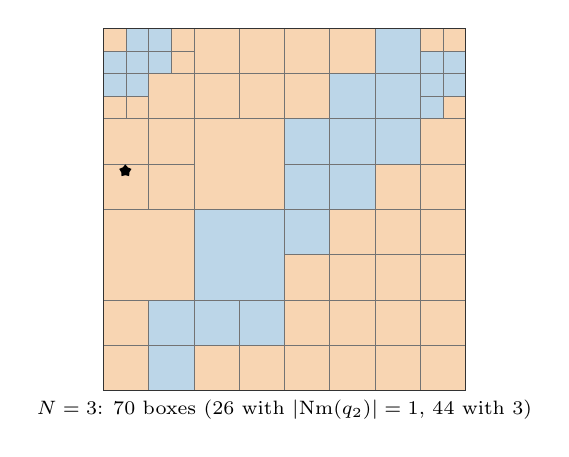
\begin{tikzpicture}[scale=4.6]
\fill[regB!30] (0.9375,0.9375) rectangle (1,1);
\fill[regA!30] (0.9375,0.875) rectangle (1,0.9375);
\fill[regB!30] (0.875,0.9375) rectangle (0.9375,1);
\fill[regA!30] (0.875,0.875) rectangle (0.9375,0.9375);
\fill[regA!30] (0.9375,0.8125) rectangle (1,0.875);
\fill[regB!30] (0.9375,0.75) rectangle (1,0.8125);
\fill[regA!30] (0.875,0.8125) rectangle (0.9375,0.875);
\fill[regA!30] (0.875,0.75) rectangle (0.9375,0.8125);
\fill[regA!30] (0.75,0.875) rectangle (0.875,1);
\fill[regA!30] (0.75,0.75) rectangle (0.875,0.875);
\fill[regB!30] (0.875,0.625) rectangle (1,0.75);
\fill[regB!30] (0.875,0.5) rectangle (1,0.625);
\fill[regA!30] (0.75,0.625) rectangle (0.875,0.75);
\fill[regB!30] (0.75,0.5) rectangle (0.875,0.625);
\fill[regB!30] (0.625,0.875) rectangle (0.75,1);
\fill[regA!30] (0.625,0.75) rectangle (0.75,0.875);
\fill[regB!30] (0.5,0.875) rectangle (0.625,1);
\fill[regB!30] (0.5,0.75) rectangle (0.625,0.875);
\fill[regA!30] (0.625,0.625) rectangle (0.75,0.75);
\fill[regA!30] (0.625,0.5) rectangle (0.75,0.625);
\fill[regA!30] (0.5,0.625) rectangle (0.625,0.75);
\fill[regA!30] (0.5,0.5) rectangle (0.625,0.625);
\fill[regB!30] (0.875,0.375) rectangle (1,0.5);
\fill[regB!30] (0.875,0.25) rectangle (1,0.375);
\fill[regB!30] (0.75,0.375) rectangle (0.875,0.5);
\fill[regB!30] (0.75,0.25) rectangle (0.875,0.375);
\fill[regB!30] (0.875,0.125) rectangle (1,0.25);
\fill[regB!30] (0.875,0) rectangle (1,0.125);
\fill[regB!30] (0.75,0.125) rectangle (0.875,0.25);
\fill[regB!30] (0.75,0) rectangle (0.875,0.125);
\fill[regB!30] (0.625,0.375) rectangle (0.75,0.5);
\fill[regB!30] (0.625,0.25) rectangle (0.75,0.375);
\fill[regA!30] (0.5,0.375) rectangle (0.625,0.5);
\fill[regB!30] (0.5,0.25) rectangle (0.625,0.375);
\fill[regB!30] (0.625,0.125) rectangle (0.75,0.25);
\fill[regB!30] (0.625,0) rectangle (0.75,0.125);
\fill[regB!30] (0.5,0.125) rectangle (0.625,0.25);
\fill[regB!30] (0.5,0) rectangle (0.625,0.125);
\fill[regB!30] (0.375,0.875) rectangle (0.5,1);
\fill[regB!30] (0.375,0.75) rectangle (0.5,0.875);
\fill[regB!30] (0.25,0.875) rectangle (0.375,1);
\fill[regB!30] (0.25,0.75) rectangle (0.375,0.875);
\fill[regB!30] (0.25,0.5) rectangle (0.5,0.75);
\fill[regB!30] (0.1875,0.9375) rectangle (0.25,1);
\fill[regB!30] (0.1875,0.875) rectangle (0.25,0.9375);
\fill[regA!30] (0.125,0.9375) rectangle (0.1875,1);
\fill[regA!30] (0.125,0.875) rectangle (0.1875,0.9375);
\fill[regB!30] (0.125,0.75) rectangle (0.25,0.875);
\fill[regA!30] (0.0625,0.9375) rectangle (0.125,1);
\fill[regA!30] (0.0625,0.875) rectangle (0.125,0.9375);
\fill[regB!30] (0,0.9375) rectangle (0.0625,1);
\fill[regA!30] (0,0.875) rectangle (0.0625,0.9375);
\fill[regA!30] (0.0625,0.8125) rectangle (0.125,0.875);
\fill[regB!30] (0.0625,0.75) rectangle (0.125,0.8125);
\fill[regA!30] (0,0.8125) rectangle (0.0625,0.875);
\fill[regB!30] (0,0.75) rectangle (0.0625,0.8125);
\fill[regB!30] (0.125,0.625) rectangle (0.25,0.75);
\fill[regB!30] (0.125,0.5) rectangle (0.25,0.625);
\fill[regB!30] (0,0.625) rectangle (0.125,0.75);
\fill[regB!30] (0,0.5) rectangle (0.125,0.625);
\fill[regA!30] (0.25,0.25) rectangle (0.5,0.5);
\fill[regA!30] (0.375,0.125) rectangle (0.5,0.25);
\fill[regB!30] (0.375,0) rectangle (0.5,0.125);
\fill[regA!30] (0.25,0.125) rectangle (0.375,0.25);
\fill[regB!30] (0.25,0) rectangle (0.375,0.125);
\fill[regB!30] (0,0.25) rectangle (0.25,0.5);
\fill[regA!30] (0.125,0.125) rectangle (0.25,0.25);
\fill[regA!30] (0.125,0) rectangle (0.25,0.125);
\fill[regB!30] (0,0.125) rectangle (0.125,0.25);
\fill[regB!30] (0,0) rectangle (0.125,0.125);
\draw[black!55, line width=0.2pt] (0.9375,0.9375) rectangle (1,1);
\draw[black!55, line width=0.2pt] (0.9375,0.875) rectangle (1,0.9375);
\draw[black!55, line width=0.2pt] (0.875,0.9375) rectangle (0.9375,1);
\draw[black!55, line width=0.2pt] (0.875,0.875) rectangle (0.9375,0.9375);
\draw[black!55, line width=0.2pt] (0.9375,0.8125) rectangle (1,0.875);
\draw[black!55, line width=0.2pt] (0.9375,0.75) rectangle (1,0.8125);
\draw[black!55, line width=0.2pt] (0.875,0.8125) rectangle (0.9375,0.875);
\draw[black!55, line width=0.2pt] (0.875,0.75) rectangle (0.9375,0.8125);
\draw[black!55, line width=0.2pt] (0.75,0.875) rectangle (0.875,1);
\draw[black!55, line width=0.2pt] (0.75,0.75) rectangle (0.875,0.875);
\draw[black!55, line width=0.2pt] (0.875,0.625) rectangle (1,0.75);
\draw[black!55, line width=0.2pt] (0.875,0.5) rectangle (1,0.625);
\draw[black!55, line width=0.2pt] (0.75,0.625) rectangle (0.875,0.75);
\draw[black!55, line width=0.2pt] (0.75,0.5) rectangle (0.875,0.625);
\draw[black!55, line width=0.2pt] (0.625,0.875) rectangle (0.75,1);
\draw[black!55, line width=0.2pt] (0.625,0.75) rectangle (0.75,0.875);
\draw[black!55, line width=0.2pt] (0.5,0.875) rectangle (0.625,1);
\draw[black!55, line width=0.2pt] (0.5,0.75) rectangle (0.625,0.875);
\draw[black!55, line width=0.2pt] (0.625,0.625) rectangle (0.75,0.75);
\draw[black!55, line width=0.2pt] (0.625,0.5) rectangle (0.75,0.625);
\draw[black!55, line width=0.2pt] (0.5,0.625) rectangle (0.625,0.75);
\draw[black!55, line width=0.2pt] (0.5,0.5) rectangle (0.625,0.625);
\draw[black!55, line width=0.2pt] (0.875,0.375) rectangle (1,0.5);
\draw[black!55, line width=0.2pt] (0.875,0.25) rectangle (1,0.375);
\draw[black!55, line width=0.2pt] (0.75,0.375) rectangle (0.875,0.5);
\draw[black!55, line width=0.2pt] (0.75,0.25) rectangle (0.875,0.375);
\draw[black!55, line width=0.2pt] (0.875,0.125) rectangle (1,0.25);
\draw[black!55, line width=0.2pt] (0.875,0) rectangle (1,0.125);
\draw[black!55, line width=0.2pt] (0.75,0.125) rectangle (0.875,0.25);
\draw[black!55, line width=0.2pt] (0.75,0) rectangle (0.875,0.125);
\draw[black!55, line width=0.2pt] (0.625,0.375) rectangle (0.75,0.5);
\draw[black!55, line width=0.2pt] (0.625,0.25) rectangle (0.75,0.375);
\draw[black!55, line width=0.2pt] (0.5,0.375) rectangle (0.625,0.5);
\draw[black!55, line width=0.2pt] (0.5,0.25) rectangle (0.625,0.375);
\draw[black!55, line width=0.2pt] (0.625,0.125) rectangle (0.75,0.25);
\draw[black!55, line width=0.2pt] (0.625,0) rectangle (0.75,0.125);
\draw[black!55, line width=0.2pt] (0.5,0.125) rectangle (0.625,0.25);
\draw[black!55, line width=0.2pt] (0.5,0) rectangle (0.625,0.125);
\draw[black!55, line width=0.2pt] (0.375,0.875) rectangle (0.5,1);
\draw[black!55, line width=0.2pt] (0.375,0.75) rectangle (0.5,0.875);
\draw[black!55, line width=0.2pt] (0.25,0.875) rectangle (0.375,1);
\draw[black!55, line width=0.2pt] (0.25,0.75) rectangle (0.375,0.875);
\draw[black!55, line width=0.2pt] (0.25,0.5) rectangle (0.5,0.75);
\draw[black!55, line width=0.2pt] (0.1875,0.9375) rectangle (0.25,1);
\draw[black!55, line width=0.2pt] (0.1875,0.875) rectangle (0.25,0.9375);
\draw[black!55, line width=0.2pt] (0.125,0.9375) rectangle (0.1875,1);
\draw[black!55, line width=0.2pt] (0.125,0.875) rectangle (0.1875,0.9375);
\draw[black!55, line width=0.2pt] (0.125,0.75) rectangle (0.25,0.875);
\draw[black!55, line width=0.2pt] (0.0625,0.9375) rectangle (0.125,1);
\draw[black!55, line width=0.2pt] (0.0625,0.875) rectangle (0.125,0.9375);
\draw[black!55, line width=0.2pt] (0,0.9375) rectangle (0.0625,1);
\draw[black!55, line width=0.2pt] (0,0.875) rectangle (0.0625,0.9375);
\draw[black!55, line width=0.2pt] (0.0625,0.8125) rectangle (0.125,0.875);
\draw[black!55, line width=0.2pt] (0.0625,0.75) rectangle (0.125,0.8125);
\draw[black!55, line width=0.2pt] (0,0.8125) rectangle (0.0625,0.875);
\draw[black!55, line width=0.2pt] (0,0.75) rectangle (0.0625,0.8125);
\draw[black!55, line width=0.2pt] (0.125,0.625) rectangle (0.25,0.75);
\draw[black!55, line width=0.2pt] (0.125,0.5) rectangle (0.25,0.625);
\draw[black!55, line width=0.2pt] (0,0.625) rectangle (0.125,0.75);
\draw[black!55, line width=0.2pt] (0,0.5) rectangle (0.125,0.625);
\draw[black!55, line width=0.2pt] (0.25,0.25) rectangle (0.5,0.5);
\draw[black!55, line width=0.2pt] (0.375,0.125) rectangle (0.5,0.25);
\draw[black!55, line width=0.2pt] (0.375,0) rectangle (0.5,0.125);
\draw[black!55, line width=0.2pt] (0.25,0.125) rectangle (0.375,0.25);
\draw[black!55, line width=0.2pt] (0.25,0) rectangle (0.375,0.125);
\draw[black!55, line width=0.2pt] (0,0.25) rectangle (0.25,0.5);
\draw[black!55, line width=0.2pt] (0.125,0.125) rectangle (0.25,0.25);
\draw[black!55, line width=0.2pt] (0.125,0) rectangle (0.25,0.125);
\draw[black!55, line width=0.2pt] (0,0.125) rectangle (0.125,0.25);
\draw[black!55, line width=0.2pt] (0,0) rectangle (0.125,0.125);
\draw[black!80] (0,0) rectangle (1,1);
\node[star, star points=5, fill=black, inner sep=1.1pt] at (0.0606,0.6061) {};
\node[font=\scriptsize, below] at (0.5,0) {$N=3$: 70 boxes (26 with $|\mathrm{Nm}(q_2)|=1$, 44 with $3$)};
\end{tikzpicture}

\caption{Sections of coverings of $\overline D$ for $K=\Q(t)$, $t^3-t^2-2t-3=0$ ($d=-327$), by
the plane $a_3=15/33$, drawn in the lattice coordinates $(a_1,a_2)\in[0,1]^2$ (so $\overline D$
is the unit cube); each square is the section of a cubic box. The star is
$x_0=\frac{2}{33}+\frac{20}{33}t+\frac{15}{33}t^2$. Left: search with $N=1$ and maximal depth
$6$; the shaded boxes lie in regions with unit denominator, the red ones could not be certified.
Right: the certificate, with $N=3$; boxes are shaded according to the norm of the denominator of
the region containing them, $1$ (blue) or $3$ (orange).}
\label{fig:slices}
\end{figure}

\begin{figure}[ht]
\centering
% generated by writeup/gen_regions.py; do not edit by hand
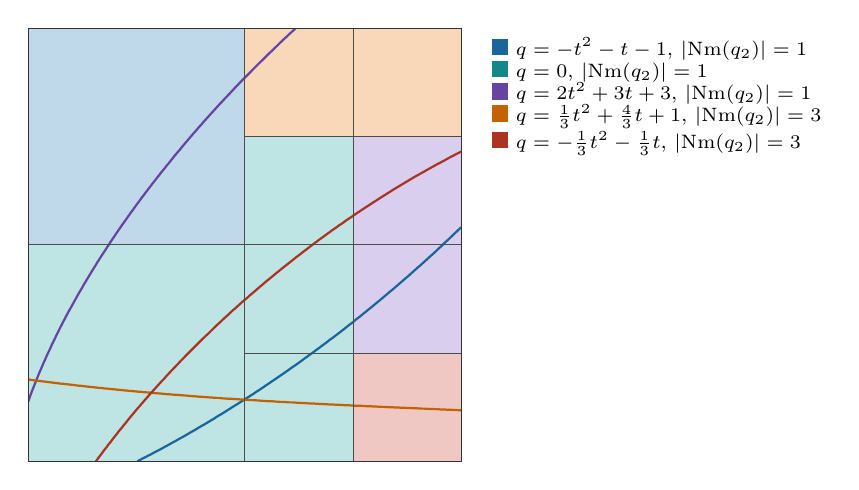
\begin{tikzpicture}[scale=22.0]
\begin{scope}\clip (0.75,0.75) rectangle (1,1);
\fill[zD!28] (0.9375,0.9375) rectangle (1,1);
\fill[zC!28] (0.9375,0.875) rectangle (1,0.9375);
\fill[zD!28] (0.875,0.9375) rectangle (0.9375,1);
\fill[zB!28] (0.875,0.875) rectangle (0.9375,0.9375);
\fill[zC!28] (0.9375,0.8125) rectangle (1,0.875);
\fill[zE!28] (0.9375,0.75) rectangle (1,0.8125);
\fill[zB!28] (0.875,0.8125) rectangle (0.9375,0.875);
\fill[zB!28] (0.875,0.75) rectangle (0.9375,0.8125);
\fill[zA!28] (0.75,0.875) rectangle (0.875,1);
\fill[zB!28] (0.75,0.75) rectangle (0.875,0.875);
\draw[zA!85!black, thick] (1,0.8852) -- (0.999,0.8842) -- (0.998,0.8833) -- (0.997,0.8823) -- (0.9959,0.8813) -- (0.9949,0.8803) -- (0.9938,0.8793) -- (0.9928,0.8783) -- (0.9917,0.8773) -- (0.9906,0.8763) -- (0.9896,0.8753) -- (0.9885,0.8742) -- (0.9875,0.8733) -- (0.9865,0.8724) -- (0.9855,0.8714) -- (0.9845,0.8705) -- (0.9835,0.8696) -- (0.9825,0.8687) -- (0.9814,0.8677) -- (0.9803,0.8667) -- (0.9792,0.8657) -- (0.9781,0.8647) -- (0.977,0.8637) -- (0.976,0.8628) -- (0.9749,0.8619) -- (0.9739,0.861) -- (0.9729,0.8601) -- (0.9719,0.8592) -- (0.9708,0.8582) -- (0.9697,0.8572) -- (0.9685,0.8562) -- (0.9674,0.8553) -- (0.9664,0.8544) -- (0.9654,0.8535) -- (0.9644,0.8527) -- (0.9633,0.8517) -- (0.9621,0.8507) -- (0.961,0.8497) -- (0.9599,0.8488) -- (0.9589,0.848) -- (0.9579,0.8471) -- (0.9568,0.8462) -- (0.9556,0.8452) -- (0.9544,0.8442) -- (0.9534,0.8433) -- (0.9524,0.8425) -- (0.9514,0.8417) -- (0.9502,0.8407) -- (0.949,0.8397) -- (0.9479,0.8388) -- (0.9469,0.838) -- (0.9459,0.8372) -- (0.9447,0.8362) -- (0.9434,0.8352) -- (0.9424,0.8343) -- (0.9414,0.8335) -- (0.9403,0.8327) -- (0.939,0.8317) -- (0.9379,0.8307) -- (0.9369,0.8299) -- (0.9359,0.8292) -- (0.9346,0.8282) -- (0.9334,0.8272) -- (0.9324,0.8264) -- (0.9314,0.8256) -- (0.9301,0.8246) -- (0.9289,0.8237) -- (0.9279,0.8229) -- (0.9268,0.8221) -- (0.9255,0.8211) -- (0.9243,0.8203) -- (0.9233,0.8195) -- (0.9222,0.8186) -- (0.9208,0.8176) -- (0.9198,0.8169) -- (0.9188,0.8161) -- (0.9175,0.8151) -- (0.9163,0.8143) -- (0.9153,0.8135) -- (0.9141,0.8126) -- (0.9128,0.8117) -- (0.9118,0.811) -- (0.9106,0.8101) -- (0.9093,0.8092) -- (0.9083,0.8084) -- (0.9072,0.8076) -- (0.9058,0.8066) -- (0.9048,0.8059) -- (0.9037,0.8051) -- (0.9023,0.8042) -- (0.9013,0.8035) -- (0.9001,0.8026) -- (0.8988,0.8017) -- (0.8978,0.801) -- (0.8965,0.8001) -- (0.8953,0.7993) -- (0.8943,0.7986) -- (0.8929,0.7976) -- (0.8918,0.7969) -- (0.8906,0.7961) -- (0.8893,0.7952) -- (0.8883,0.7945) -- (0.8869,0.7936) -- (0.8858,0.7928) -- (0.8847,0.7921) -- (0.8833,0.7911) -- (0.8823,0.7905) -- (0.8809,0.7896) -- (0.8798,0.7888) -- (0.8786,0.7881) -- (0.8773,0.7872) -- (0.8763,0.7866) -- (0.8747,0.7856) -- (0.8737,0.7849) -- (0.8724,0.7841) -- (0.8712,0.7833) -- (0.87,0.7826) -- (0.8687,0.7818) -- (0.8676,0.7811) -- (0.8662,0.7802) -- (0.8652,0.7796) -- (0.8637,0.7786) -- (0.8627,0.778) -- (0.8612,0.7771) -- (0.8602,0.7765) -- (0.8587,0.7756) -- (0.8577,0.7749) -- (0.8562,0.774) -- (0.8552,0.7734) -- (0.8537,0.7725) -- (0.8527,0.7719) -- (0.8512,0.771) -- (0.8502,0.7705) -- (0.8487,0.7696) -- (0.8477,0.769) -- (0.8462,0.7681) -- (0.8452,0.7675) -- (0.8437,0.7667) -- (0.8426,0.766) -- (0.8412,0.7652) -- (0.84,0.7645) -- (0.8387,0.7638) -- (0.8373,0.763) -- (0.8362,0.7624) -- (0.8347,0.7615) -- (0.8337,0.761) -- (0.8322,0.7602) -- (0.831,0.7595) -- (0.8297,0.7588) -- (0.8282,0.758) -- (0.8272,0.7574) -- (0.8257,0.7566) -- (0.8245,0.756) -- (0.8231,0.7553) -- (0.8217,0.7545) -- (0.8206,0.7539) -- (0.8191,0.7532) -- (0.8179,0.7525) -- (0.8166,0.7519) -- (0.8151,0.7511) -- (0.814,0.7505) -- (0.813,0.75);
\draw[zC!85!black, thick] (0.75,0.7845) -- (0.7505,0.7859) -- (0.751,0.7873) -- (0.7515,0.7887) -- (0.752,0.7901) -- (0.7526,0.7916) -- (0.7532,0.7931) -- (0.7538,0.7946) -- (0.7544,0.7961) -- (0.755,0.7976) -- (0.7555,0.7989) -- (0.756,0.8001) -- (0.7566,0.8016) -- (0.7573,0.8031) -- (0.7579,0.8046) -- (0.7585,0.806) -- (0.759,0.8072) -- (0.7597,0.8086) -- (0.7603,0.8101) -- (0.761,0.8116) -- (0.7615,0.8127) -- (0.7622,0.8141) -- (0.7629,0.8156) -- (0.7635,0.817) -- (0.764,0.8181) -- (0.7648,0.8196) -- (0.7655,0.8211) -- (0.766,0.8222) -- (0.7667,0.8236) -- (0.7675,0.8252) -- (0.768,0.8263) -- (0.7687,0.8277) -- (0.7695,0.8292) -- (0.77,0.8302) -- (0.7708,0.8317) -- (0.7715,0.8331) -- (0.7721,0.8342) -- (0.7729,0.8357) -- (0.7735,0.8368) -- (0.7743,0.8382) -- (0.7751,0.8396) -- (0.7757,0.8407) -- (0.7765,0.8422) -- (0.7771,0.8432) -- (0.7779,0.8447) -- (0.7786,0.8459) -- (0.7793,0.8472) -- (0.7801,0.8485) -- (0.7808,0.8497) -- (0.7816,0.8511) -- (0.7822,0.8522) -- (0.7831,0.8536) -- (0.7837,0.8547) -- (0.7846,0.8561) -- (0.7852,0.8572) -- (0.7861,0.8586) -- (0.7867,0.8597) -- (0.7876,0.8611) -- (0.7883,0.8622) -- (0.7891,0.8635) -- (0.7898,0.8647) -- (0.7906,0.8659) -- (0.7914,0.8672) -- (0.7921,0.8683) -- (0.793,0.8697) -- (0.7937,0.8707) -- (0.7946,0.8721) -- (0.7953,0.8732) -- (0.7961,0.8744) -- (0.797,0.8758) -- (0.7976,0.8768) -- (0.7986,0.8782) -- (0.7993,0.8793) -- (0.8001,0.8804) -- (0.801,0.8818) -- (0.8017,0.8828) -- (0.8026,0.8841) -- (0.8034,0.8853) -- (0.8041,0.8863) -- (0.8051,0.8877) -- (0.8059,0.8888) -- (0.8066,0.8898) -- (0.8076,0.8913) -- (0.8084,0.8923) -- (0.8091,0.8934) -- (0.8101,0.8947) -- (0.8109,0.8958) -- (0.8116,0.8968) -- (0.8126,0.8982) -- (0.8134,0.8993) -- (0.8142,0.9003) -- (0.8151,0.9016) -- (0.816,0.9028) -- (0.8168,0.9038) -- (0.8176,0.9049) -- (0.8186,0.9062) -- (0.8194,0.9073) -- (0.8202,0.9083) -- (0.8211,0.9095) -- (0.8221,0.9108) -- (0.8229,0.9118) -- (0.8237,0.9128) -- (0.8246,0.914) -- (0.8257,0.9153) -- (0.8264,0.9163) -- (0.8272,0.9173) -- (0.8282,0.9185) -- (0.8292,0.9197) -- (0.83,0.9208) -- (0.8309,0.9218) -- (0.8317,0.9228) -- (0.8327,0.9241) -- (0.8337,0.9253) -- (0.8345,0.9264) -- (0.8354,0.9274) -- (0.8362,0.9284) -- (0.8372,0.9295) -- (0.8382,0.9307) -- (0.8391,0.9319) -- (0.84,0.9329) -- (0.8408,0.9339) -- (0.8417,0.9349) -- (0.8427,0.9361) -- (0.8437,0.9373) -- (0.8447,0.9384) -- (0.8455,0.9394) -- (0.8464,0.9404) -- (0.8473,0.9414) -- (0.8482,0.9425) -- (0.8492,0.9436) -- (0.8502,0.9447) -- (0.8512,0.9459) -- (0.8521,0.9469) -- (0.853,0.9479) -- (0.8539,0.9489) -- (0.8548,0.9499) -- (0.8557,0.9509) -- (0.8567,0.952) -- (0.8577,0.9531) -- (0.8587,0.9542) -- (0.8597,0.9553) -- (0.8607,0.9564) -- (0.8617,0.9574) -- (0.8626,0.9584) -- (0.8635,0.9594) -- (0.8645,0.9604) -- (0.8654,0.9614) -- (0.8664,0.9624) -- (0.8673,0.9634) -- (0.8683,0.9644) -- (0.8692,0.9655) -- (0.8702,0.9665) -- (0.8712,0.9675) -- (0.8722,0.9686) -- (0.8732,0.9696) -- (0.8742,0.9707) -- (0.8753,0.9717) -- (0.8763,0.9727) -- (0.8773,0.9737) -- (0.8783,0.9747) -- (0.8793,0.9758) -- (0.8803,0.9768) -- (0.8813,0.9778) -- (0.8823,0.9788) -- (0.8833,0.9798) -- (0.8843,0.9808) -- (0.8853,0.9817) -- (0.8863,0.9827) -- (0.8873,0.9837) -- (0.8883,0.9847) -- (0.8893,0.9857) -- (0.8903,0.9866) -- (0.8913,0.9876) -- (0.8923,0.9886) -- (0.8933,0.9895) -- (0.8943,0.9905) -- (0.8953,0.9915) -- (0.8964,0.9925) -- (0.8974,0.9935) -- (0.8985,0.9945) -- (0.8996,0.9955) -- (0.9006,0.9965) -- (0.9017,0.9975) -- (0.9028,0.9985) -- (0.9038,0.9994) -- (0.9044,1);
\draw[zD!85!black, thick] (1,0.7795) -- (0.9985,0.7795) -- (0.9975,0.7796) -- (0.996,0.7796) -- (0.9945,0.7797) -- (0.993,0.7798) -- (0.9915,0.7798) -- (0.99,0.7799) -- (0.9885,0.7799) -- (0.987,0.78) -- (0.9858,0.7801) -- (0.9845,0.7801) -- (0.983,0.7802) -- (0.9815,0.7802) -- (0.98,0.7803) -- (0.9785,0.7804) -- (0.977,0.7804) -- (0.9755,0.7805) -- (0.974,0.7806) -- (0.9729,0.7806) -- (0.9714,0.7807) -- (0.9699,0.7807) -- (0.9684,0.7808) -- (0.9669,0.7809) -- (0.9654,0.7809) -- (0.9639,0.781) -- (0.9624,0.7811) -- (0.9614,0.7811) -- (0.9599,0.7812) -- (0.9584,0.7812) -- (0.9569,0.7813) -- (0.9554,0.7814) -- (0.9539,0.7814) -- (0.9524,0.7815) -- (0.9511,0.7816) -- (0.9499,0.7816) -- (0.9484,0.7817) -- (0.9469,0.7818) -- (0.9454,0.7818) -- (0.9439,0.7819) -- (0.9424,0.782) -- (0.9409,0.782) -- (0.9399,0.7821) -- (0.9384,0.7821) -- (0.9369,0.7822) -- (0.9354,0.7823) -- (0.9339,0.7824) -- (0.9324,0.7824) -- (0.9309,0.7825) -- (0.9295,0.7826) -- (0.9284,0.7826) -- (0.9269,0.7827) -- (0.9254,0.7828) -- (0.9238,0.7828) -- (0.9223,0.7829) -- (0.9208,0.783) -- (0.9193,0.7831) -- (0.9183,0.7831) -- (0.9168,0.7832) -- (0.9153,0.7833) -- (0.9138,0.7833) -- (0.9123,0.7834) -- (0.9108,0.7835) -- (0.9096,0.7836) -- (0.9083,0.7836) -- (0.9068,0.7837) -- (0.9053,0.7838) -- (0.9038,0.7839) -- (0.9023,0.784) -- (0.9008,0.784) -- (0.8998,0.7841) -- (0.8983,0.7842) -- (0.8968,0.7843) -- (0.8953,0.7843) -- (0.8938,0.7844) -- (0.8923,0.7845) -- (0.8913,0.7846) -- (0.8898,0.7847) -- (0.8883,0.7847) -- (0.8868,0.7848) -- (0.8853,0.7849) -- (0.8838,0.785) -- (0.8828,0.7851) -- (0.8813,0.7852) -- (0.8798,0.7853) -- (0.8783,0.7853) -- (0.8768,0.7854) -- (0.8753,0.7855) -- (0.8742,0.7856) -- (0.8727,0.7857) -- (0.8712,0.7858) -- (0.8697,0.7859) -- (0.8682,0.786) -- (0.8669,0.7861) -- (0.8657,0.7861) -- (0.8642,0.7862) -- (0.8627,0.7863) -- (0.8612,0.7864) -- (0.8597,0.7866) -- (0.8587,0.7866) -- (0.8572,0.7867) -- (0.8557,0.7868) -- (0.8542,0.7869) -- (0.8527,0.787) -- (0.8517,0.7871) -- (0.8502,0.7872) -- (0.8487,0.7873) -- (0.8472,0.7874) -- (0.8457,0.7876) -- (0.8447,0.7876) -- (0.8432,0.7877) -- (0.8417,0.7879) -- (0.8402,0.788) -- (0.8388,0.7881) -- (0.8377,0.7882) -- (0.8362,0.7883) -- (0.8347,0.7884) -- (0.8332,0.7885) -- (0.8322,0.7886) -- (0.8307,0.7887) -- (0.8292,0.7888) -- (0.8277,0.789) -- (0.8264,0.7891) -- (0.8252,0.7892) -- (0.8236,0.7893) -- (0.8221,0.7894) -- (0.8206,0.7896) -- (0.8196,0.7897) -- (0.8181,0.7898) -- (0.8166,0.7899) -- (0.8151,0.7901) -- (0.8141,0.7901) -- (0.8126,0.7903) -- (0.8111,0.7904) -- (0.8096,0.7906) -- (0.8086,0.7906) -- (0.8071,0.7908) -- (0.8056,0.7909) -- (0.8041,0.7911) -- (0.8031,0.7912) -- (0.8016,0.7913) -- (0.8001,0.7915) -- (0.7989,0.7916) -- (0.7976,0.7917) -- (0.7961,0.7919) -- (0.7946,0.792) -- (0.7936,0.7921) -- (0.7921,0.7923) -- (0.7906,0.7924) -- (0.7891,0.7926) -- (0.7881,0.7927) -- (0.7866,0.7929) -- (0.7851,0.793) -- (0.7841,0.7931) -- (0.7826,0.7933) -- (0.7811,0.7935) -- (0.7798,0.7936) -- (0.7786,0.7937) -- (0.7771,0.7939) -- (0.7756,0.7941) -- (0.7745,0.7942) -- (0.773,0.7944) -- (0.7715,0.7945) -- (0.7705,0.7947) -- (0.769,0.7948) -- (0.7675,0.795) -- (0.7665,0.7951) -- (0.765,0.7953) -- (0.7635,0.7955) -- (0.7625,0.7956) -- (0.761,0.7958) -- (0.7595,0.796) -- (0.7585,0.7961) -- (0.757,0.7963) -- (0.7555,0.7965) -- (0.7545,0.7966) -- (0.753,0.7968) -- (0.7515,0.797) -- (0.7505,0.7972) -- (0.75,0.7972);
\draw[zE!85!black, thick] (0.7891,0.75) -- (0.7901,0.7514) -- (0.7909,0.7525) -- (0.7917,0.7535) -- (0.7926,0.7547) -- (0.7935,0.756) -- (0.7943,0.757) -- (0.7951,0.758) -- (0.7961,0.7594) -- (0.797,0.7605) -- (0.7978,0.7615) -- (0.7986,0.7626) -- (0.7996,0.7639) -- (0.8005,0.765) -- (0.8013,0.766) -- (0.8021,0.7671) -- (0.8031,0.7683) -- (0.8041,0.7695) -- (0.8049,0.7705) -- (0.8057,0.7715) -- (0.8066,0.7726) -- (0.8076,0.7739) -- (0.8086,0.7751) -- (0.8094,0.7761) -- (0.8103,0.7771) -- (0.8111,0.7781) -- (0.8121,0.7793) -- (0.8131,0.7805) -- (0.8141,0.7816) -- (0.8149,0.7826) -- (0.8158,0.7836) -- (0.8167,0.7846) -- (0.8176,0.7857) -- (0.8186,0.7868) -- (0.8196,0.788) -- (0.8206,0.7891) -- (0.8215,0.7901) -- (0.8224,0.7911) -- (0.8233,0.7921) -- (0.8242,0.7931) -- (0.8252,0.7942) -- (0.8262,0.7953) -- (0.8272,0.7964) -- (0.8282,0.7974) -- (0.8292,0.7985) -- (0.8301,0.7996) -- (0.8311,0.8006) -- (0.832,0.8016) -- (0.833,0.8026) -- (0.8339,0.8036) -- (0.8349,0.8046) -- (0.8358,0.8056) -- (0.8368,0.8066) -- (0.8377,0.8076) -- (0.8387,0.8086) -- (0.8397,0.8096) -- (0.8407,0.8107) -- (0.8417,0.8117) -- (0.8427,0.8127) -- (0.8437,0.8137) -- (0.8447,0.8147) -- (0.8457,0.8157) -- (0.8467,0.8167) -- (0.8477,0.8177) -- (0.8487,0.8187) -- (0.8497,0.8197) -- (0.8507,0.8207) -- (0.8517,0.8216) -- (0.8527,0.8226) -- (0.8538,0.8236) -- (0.8548,0.8246) -- (0.8559,0.8257) -- (0.8569,0.8267) -- (0.858,0.8277) -- (0.859,0.8287) -- (0.8601,0.8297) -- (0.8612,0.8307) -- (0.8622,0.8317) -- (0.8632,0.8326) -- (0.8642,0.8335) -- (0.8652,0.8344) -- (0.8662,0.8353) -- (0.8672,0.8363) -- (0.8682,0.8372) -- (0.8694,0.8382) -- (0.8705,0.8392) -- (0.8716,0.8402) -- (0.8727,0.8412) -- (0.8737,0.8421) -- (0.8747,0.843) -- (0.8758,0.8439) -- (0.8768,0.8447) -- (0.8778,0.8457) -- (0.879,0.8467) -- (0.8802,0.8477) -- (0.8813,0.8486) -- (0.8823,0.8495) -- (0.8833,0.8504) -- (0.8843,0.8512) -- (0.8855,0.8522) -- (0.8866,0.8532) -- (0.8878,0.8542) -- (0.8888,0.855) -- (0.8898,0.8558) -- (0.8909,0.8567) -- (0.8921,0.8577) -- (0.8933,0.8587) -- (0.8943,0.8595) -- (0.8953,0.8603) -- (0.8964,0.8612) -- (0.8976,0.8622) -- (0.8988,0.8631) -- (0.8998,0.8639) -- (0.9008,0.8647) -- (0.9021,0.8657) -- (0.9033,0.8667) -- (0.9043,0.8675) -- (0.9053,0.8683) -- (0.9066,0.8692) -- (0.9078,0.8702) -- (0.9088,0.871) -- (0.9098,0.8717) -- (0.9111,0.8727) -- (0.9123,0.8736) -- (0.9133,0.8744) -- (0.9145,0.8753) -- (0.9158,0.8763) -- (0.9168,0.877) -- (0.9178,0.8778) -- (0.9192,0.8788) -- (0.9203,0.8796) -- (0.9213,0.8803) -- (0.9226,0.8813) -- (0.9238,0.8821) -- (0.9248,0.8829) -- (0.9261,0.8838) -- (0.9274,0.8847) -- (0.9284,0.8854) -- (0.9296,0.8863) -- (0.9309,0.8871) -- (0.9319,0.8878) -- (0.9332,0.8888) -- (0.9344,0.8896) -- (0.9354,0.8903) -- (0.9369,0.8913) -- (0.9379,0.892) -- (0.9391,0.8928) -- (0.9404,0.8937) -- (0.9414,0.8943) -- (0.9428,0.8953) -- (0.9439,0.896) -- (0.9451,0.8968) -- (0.9464,0.8976) -- (0.9474,0.8983) -- (0.9489,0.8993) -- (0.9499,0.8999) -- (0.9513,0.9008) -- (0.9524,0.9015) -- (0.9536,0.9023) -- (0.9549,0.9031) -- (0.956,0.9038) -- (0.9574,0.9047) -- (0.9584,0.9053) -- (0.9599,0.9063) -- (0.9609,0.9069) -- (0.9624,0.9078) -- (0.9634,0.9084) -- (0.9649,0.9093) -- (0.9659,0.9099) -- (0.9674,0.9108) -- (0.9684,0.9114) -- (0.9699,0.9123) -- (0.9709,0.9129) -- (0.9724,0.9138) -- (0.9734,0.9144) -- (0.9749,0.9152) -- (0.976,0.9158) -- (0.9775,0.9167) -- (0.9787,0.9173) -- (0.98,0.9181) -- (0.9813,0.9188) -- (0.9825,0.9195) -- (0.984,0.9203) -- (0.985,0.9209) -- (0.9865,0.9217) -- (0.9877,0.9223) -- (0.989,0.923) -- (0.9905,0.9238) -- (0.9915,0.9244) -- (0.993,0.9252) -- (0.9943,0.9259) -- (0.9955,0.9265) -- (0.997,0.9273) -- (0.9981,0.9279) -- (0.9995,0.9285) -- (1,0.9288);
\draw[black!70, line width=0.3pt] (0.9375,0.9375) rectangle (1,1);
\draw[black!70, line width=0.3pt] (0.9375,0.875) rectangle (1,0.9375);
\draw[black!70, line width=0.3pt] (0.875,0.9375) rectangle (0.9375,1);
\draw[black!70, line width=0.3pt] (0.875,0.875) rectangle (0.9375,0.9375);
\draw[black!70, line width=0.3pt] (0.9375,0.8125) rectangle (1,0.875);
\draw[black!70, line width=0.3pt] (0.9375,0.75) rectangle (1,0.8125);
\draw[black!70, line width=0.3pt] (0.875,0.8125) rectangle (0.9375,0.875);
\draw[black!70, line width=0.3pt] (0.875,0.75) rectangle (0.9375,0.8125);
\draw[black!70, line width=0.3pt] (0.75,0.875) rectangle (0.875,1);
\draw[black!70, line width=0.3pt] (0.75,0.75) rectangle (0.875,0.875);
\end{scope}
\draw[black!80] (0.75,0.75) rectangle (1,1);
\node[anchor=north west, font=\scriptsize, align=left] at (1.012,1) {\textcolor{zA!85!black}{\rule{6pt}{6pt}}\ $q=-t^{2} - t - 1$, $|\mathrm{Nm}(q_2)|=1$\\ \textcolor{zB!85!black}{\rule{6pt}{6pt}}\ $q=0$, $|\mathrm{Nm}(q_2)|=1$\\ \textcolor{zC!85!black}{\rule{6pt}{6pt}}\ $q=2 t^{2} + 3 t + 3$, $|\mathrm{Nm}(q_2)|=1$\\ \textcolor{zD!85!black}{\rule{6pt}{6pt}}\ $q=\frac{1}{3} t^{2} + \frac{4}{3} t + 1$, $|\mathrm{Nm}(q_2)|=3$\\ \textcolor{zE!85!black}{\rule{6pt}{6pt}}\ $q=-\frac{1}{3} t^{2} - \frac{1}{3} t$, $|\mathrm{Nm}(q_2)|=3$};
\end{tikzpicture}

\caption{A detail of Figure~\ref{fig:slices} (right): the square
$[\frac34,1]\times[\frac34,1]$ of the plane $a_3=15/33$. Each box is shaded with the color of a
region $V(q)$ containing it, and the section of the boundary $|\Nm(x-q)|=|\Nm(q_2)|^{-1}$ of that
region is drawn in the same color (where it meets the square). By Lemma~\ref{lem:box} a box is
certified when the bound for the whole cube, not only its section, is below the threshold.}
\label{fig:zoom3}
\end{figure}

\begin{proposition}\label{prop:terminate}
If $K$ is $N$-smooth Euclidean, then there are a finite set $Z\subset\mathcal C_N$ and a depth
$\ell$ such that the search terminates whenever its candidate set contains $Z$ and its maximal
depth is at least $\ell$.
\end{proposition}

\begin{proof}
By compactness $\overline D$ is covered by finitely many $V(c)$, $c\in Z$, so
$\phi(x)=\min_{c\in Z}n_c|\Nm(x-\sigma(c))|$ satisfies $\phi\le1-\eta$ on $\overline D$ for some
$\eta>0$. The upper bound of Lemma~\ref{lem:box} converges to $|\Nm(x-\sigma(c))|$ uniformly as
the side $h\to0$, so for $h$ small every box passes the test for some $c\in Z$.
\end{proof}

By Theorem~\ref{thm:equiv}, a $2$-stage Euclidean field is $N$-smooth Euclidean for some $N$
(the largest denominator norm in a finite covering). Hence $\Nmin(K)$ is finite exactly for
the $2$-stage Euclidean fields, and a search whose candidate sets and maximal depth grow without
bound terminates exactly for these fields.

%=====================================================================================
\section{Exact obstructions}\label{sec:witness}

For $x\in K$ let $f(x)=\min_{g\in\cO_K}|\Nm(x-g)|$ (the minimum exists, since the values lie in
$m^{-3}\Z$ when $mx\in\cO_K$). A point with $f(x)\ge1$ is a \emph{witness}: it lies in no region
with unit denominator, so $K$ is not norm-Euclidean and $\Nmin(K)\ge2$. Since $f$ is invariant
under $x\mapsto\pm\varepsilon x$ and translation by $\cO_K$, the following lemma reduces its
computation to finitely many translates.

\begin{lemma}\label{lem:normalize}
Let $y\in\R\times\C$ with $|u|,|w|>0$ and $|\Nm(y)|<1$. There is $k\in\Z$ such that
$\varepsilon^ky=(u',w')$ satisfies $|u'|<\lambda^{1/2}$ and $|w'|<\lambda^{1/4}$.
\end{lemma}

\begin{proof}
Put $s=\log|u|$, $t=\log|w|$, so $s+2t<0$. Multiplication by $\varepsilon$ changes $(s,t)$ by
$\pm(\log\lambda,-\tfrac12\log\lambda)$, hence $s-t$ by $\pm\tfrac32\log\lambda$, and we can
choose $k$ with $|s'-t'|\le\tfrac34\log\lambda$. Then
$3s'=(s'+2t')+2(s'-t')<\tfrac32\log\lambda$ and $3t'=(s'+2t')-(s'-t')<\tfrac34\log\lambda$.
\end{proof}

\begin{figure}[t]
\centering
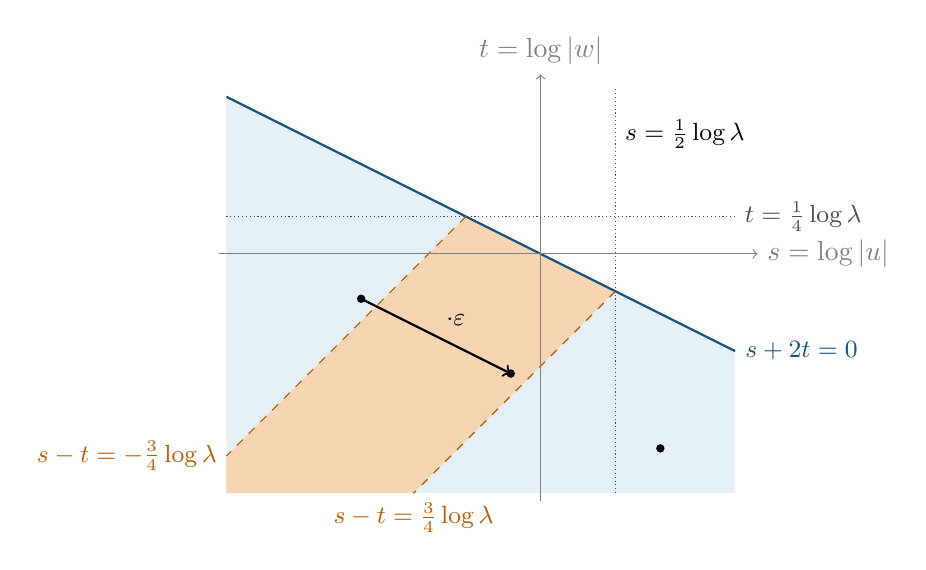
\begin{tikzpicture}[scale=0.95]
  \def\L{2.0}
  \fill[cA!12] (-4.2,2.1) -- (2.6,-1.3) -- (2.6,-3.2) -- (-4.2,-3.2) -- cycle;
  \fill[cB!30] (-1.0,0.5) -- (1.0,-0.5) -- (-1.7,-3.2) -- (-4.2,-3.2) -- (-4.2,-2.7) -- cycle;
  \draw[cA!70!black, thick] (-4.2,2.1) -- (2.6,-1.3) node[right, font=\small] {$s+2t=0$};
  \draw[cB!80!black, dashed] (-1.0,0.5) -- (-4.2,-2.7) node[left, font=\small] {$s-t=-\frac34\log\lambda$};
  \draw[cB!80!black, dashed] (1.0,-0.5) -- (-1.7,-3.2) node[below, font=\small] {$s-t=\frac34\log\lambda$};
  \draw[->, gray] (-4.3,0) -- (2.9,0) node[right] {$s=\log|u|$};
  \draw[->, gray] (0,-3.3) -- (0,2.4) node[above] {$t=\log|w|$};
  \draw[black!70, densely dotted] (1.0,-3.2) -- (1.0,2.2);
  \node[font=\small, right] at (1.0,1.6) {$s=\tfrac12\log\lambda$};
  \draw[black!70, densely dotted] (-4.2,0.5) -- (2.6,0.5) node[right, font=\small] {$t=\tfrac14\log\lambda$};
  \foreach \k in {-1,0,1} {
    \fill[black] ({-0.4+2.0*\k},{-1.6-1.0*\k}) circle (1.6pt);
  }
  \draw[->, thick] (-2.4,-0.6) -- (-0.4,-1.6) node[midway, above right, font=\small] {$\cdot\varepsilon$};
\end{tikzpicture}
\caption{Lemma~\ref{lem:normalize} in logarithmic coordinates. The condition $|\Nm(y)|<1$ is
the half-plane $s+2t<0$; the unit acts by translations parallel to its boundary, and every orbit
(dots) meets the strip $|s-t|\le\frac34\log\lambda$, whose part in the half-plane (orange) lies
in $\{s<\frac12\log\lambda,\ t<\frac14\log\lambda\}$.}
\label{fig:normalize}
\end{figure}

Let $B=\{|u|<\lambda^{1/2},|w|<\lambda^{1/4}\}$ and let $\mathcal D\subset\Z^3$ be the set of
lattice vectors $d$ such that $\sigma([0,1]^3-d)$ can meet $B\cap\{|\Nm|<1\}$; by
Lemma~\ref{lem:box} it is computable, and it is finite.

\begin{proposition}\label{prop:witness}
Let $x=a/m$ with $a\in\cO_K$ given by its lattice coordinates in $[0,m)^3$. Then $f(x)\ge1$ if
and only if $|\Nm(a'-md)|\ge m^3$ for every $d\in\mathcal D$ and every $a'\in[0,m)^3$ in the
orbit of $a$ modulo $m$ under multiplication by $\pm\varepsilon$.
\end{proposition}

\begin{proof}
If $|\Nm(x-g)|<1$, Lemma~\ref{lem:normalize} gives $k$ with $\sigma(\varepsilon^k(x-g))\in B$.
Writing $\varepsilon^kx=a'/m+h$ with $h\in\cO_K$ and $a'\in[0,m)^3$, we get
$\varepsilon^k(x-g)=a'/m-d$ with $d=\varepsilon^kg-h$, and $d\in\mathcal D$. The converse is
clear, and $\Nm(a'/m-d)=m^{-3}\Nm(a'-md)$ is computed exactly from the integral norm form.
\end{proof}

\emph{Enumerating $\mathcal D$.} A point $y\in B$ with $|\Nm(y)|<1$ and $|u|\in(2^{i-1},2^i]$
has $|w|<2^{-(i-1)/2}$. Hence $B\cap\{|\Nm|<1\}$ is covered by the boxes
$P_{i_0}=\{|u|\le2^{i_0},\ |w|\le\lambda^{1/4}\}$, with $2^{i_0}\le\lambda^{-1/2}$, and
$P_i=\{|u|\le2^i,\ |w|\le\min(\lambda^{1/4},2^{-(i-1)/2})\}$ for $i_0<i\le i_1$, with
$2^{i_1}\ge\lambda^{1/2}$. Since $\sigma([0,1]^3)$ lies in a box with half-sides $r_u,r_w$ around
its centre, the elements of $\mathcal D$ coming from $P_i$ lie in a box of volume
$\asymp(2^i+r_u)(2^{-i/2}+r_w)^2$. Summing over $i$ gives $|\mathcal D|=O(\lambda^{1/2})$, instead
of the $\asymp\lambda$ points of a box containing $B$.

\emph{The search.} The test is applied to all $a\in(\Z/m)^3$ at once. The points with
$|\Nm(a-md)|<m^3$ for some $d\in\mathcal D$ are marked, using a floating-point filter followed by
exact evaluation of the integral norm form near the threshold, and the witnesses are the
$\langle-1,\varepsilon\rangle$-orbits with no marked point. Orbits are labelled by pointer
doubling, so the cost is $O(m^3(|\mathcal D|+\log m))$ operations. The search enumerates
$\mathcal D$ in floating point (LLL and Fincke--Pohst for an ellipsoid around each piece) and
skips fields where $|\mathcal D|$ would exceed $3\cdot10^6$.

\emph{The proof.} The search alone is not a proof, since a missing element of $\mathcal D$
could produce a false witness. Every reported point is therefore re-checked by a separate
program. It bounds $\lambda$ from above in interval arithmetic, with the fundamental unit
certified by \texttt{bnfcertify}. For each piece $P_i$ it chooses a unimodular matrix $U$ by LLL
and computes, in $256$-bit interval arithmetic with $\sigma^{-1}$ given by the trace-dual basis,
an integer box in the coordinates $U^{-1}d$ that contains all $d$ with
$d\in[0,1]^3-\sigma^{-1}(P_i)$. It enumerates this box (a superset of $\mathcal D$ is harmless).
Norms are evaluated with the integral norm form in floating point, with an a priori error bound
$10^{-13}\sum|\text{terms}|$, about sixty times the standard bound, and in exact integer
arithmetic whenever the result is not decided. For small $m$ we also use a second exact test,
which needs no translates: $a/m$ is covered if and only if $a\equiv u\gamma\pmod m$ for a unit
$u$ and a generator $\gamma$ of an ideal of norm less than $m^3$. This is also the principle of
Method~I of \cite{BBT}.

This re-check confirmed all but two of the witnesses found by our searches. The exceptions were
reported by an earlier version of the search for $d=-4872$ and $d=-4952$, whose fundamental
units are very large ($\log\lambda\approx30$ and $35$) and for which that version enumerated
too few translates. For these fields $x=\tfrac12t^2$, resp.\ $\tfrac12(t+t^2)$, is in fact
covered: there is $g\in\cO_K$ with $\Nm(x-g)=-\frac12$. They are excluded from all counts
below.

The same argument bounds the smooth level from below.

\begin{proposition}\label{prop:level}
Let $x=a/m$, and for every class $c=r/\alpha$ with $n=\Nm(\alpha\cO_K)\le L$ let
$b_c=na-m\,(nr/\alpha)\in\cO_K$. If $f(b_c/(mn))\ge 1/n$ for all such $c$, then $x$ lies in no
region with centre in $\mathcal C_L$, and $\Nmin(K)>L$.
\end{proposition}

\begin{proof}
$x\in V(c+g)$ if and only if $|\Nm(x-c-g)|<1/n$, and $x-c=b_c/(mn)$. The condition
$f(b_c/(mn))\ge1/n$ is decided as in Proposition~\ref{prop:witness} with modulus $M=mn$ and
threshold $|\Nm(b'-Md)|\ge M^3/n$.
\end{proof}

If the certified covering uses $\Nmin$ equal to the largest ideal norm $N$ and a point as in
Proposition~\ref{prop:level} exists for $L=N-1$, then $\Nmin(K)=N$. When no ideal has norm in
$(1,N)$, an ordinary witness suffices.

%=====================================================================================
\section{Continued fractions}\label{sec:cf}

Given a certificate, a $2$-stage chain for $\alpha,\beta$ is found as follows. Let $x=\alpha/\beta$,
let $\xi\in\Q^3$ be its lattice coordinates, and write $\xi=\lfloor\xi\rfloor+\{\xi\}$
componentwise. The dyadic box containing $\{\xi\}$ is found by a dictionary lookup at each
depth. If its centre is $r/\alpha_0+g$, choose $u\in\pm\varepsilon^{\Z}$ with
$u\equiv r\pmod{\alpha_0}$ (it exists by Lemma~\ref{lem:classes}), and put $q_2=\alpha_0/u$ and
$q_1=\lfloor\xi\rfloor+g+(r-u)/\alpha_0$, where $\lfloor\xi\rfloor$ stands for the corresponding
element of $\cO_K$. Then
$|\Nm(x-[q_1,q_2])|<1/|\Nm(q_2)|$ and \eqref{eq:chain} holds by Proposition~\ref{prop:cooke}.
Repeating with $(r_1,r_2)$ gives the continued fraction, since $|\Nm|$ of the remainders
decreases at least every two steps.

For example, let $K=\Q(t)$ with $t^3-t^2-2t-3=0$, $d=-327$. This field is not norm-Euclidean:
$x_0=\frac{2}{33}+\frac{20}{33}t+\frac{5}{11}t^2$ satisfies $f(x_0)\ge1$, in accordance with
$M(K)=\frac{101}{99}$ \cite{CL}. There is no ideal of norm $2$, so $\Nmin(K)\ge3$; and
$3\cO_K=\mathfrak p^2\mathfrak p'$ has two prime ideals of norm $3$, which our certificate with
$N=3$ uses, so $\Nmin(K)=3$. For $x=(2+3t+5t^2)/(7-t)=(194+223t+268t^2)/277$ the algorithm gives
\[
  x=[\,t^2+t,\ 1,\ t^2-3t,\ 1,\ -t^2+t,\ t\,],
\]
from the chain with $\beta=277$ in Table~\ref{tab:cf}. The second step is a genuine $2$-stage
step: the first remainder is larger than $\beta$ in norm, the second one smaller. The last
quotient $t$ has norm $3$.

\begin{table}[ht]
\centering\small
\begin{tabular}{cccrrr}
\toprule
step & $q_1$ & $q_2$ & $|\Nm(\beta)|$ & $|\Nm(r_1)|$ & $|\Nm(r_2)|$\\
\midrule
1 & $t^2+t$ & $1$ & $21\,253\,933$ & $844\,019$ & $844\,019$\\
2 & $t^2-3t$ & $1$ & $844\,019$ & $1\,841\,496$ & $230\,187$\\
3 & $-t^2+t$ & $t$ & $230\,187$ & $76\,729$ & $0$\\
\bottomrule
\end{tabular}
\caption{The division chain behind the continued fraction of $x=(2+3t+5t^2)/(7-t)$ in the field
of discriminant $-327$.}
\label{tab:cf}
\end{table}

%=====================================================================================
\section{Results}\label{sec:results}

\subsection{The fields}\label{sec:fields}
The complex cubic fields with $|d|<5000$ were listed with PARI/GP's \texttt{nflist}
\cite{PARI}: there are $729$, and \texttt{bnfcertify} proves that exactly $550$ of them have class
number one, without assuming GRH. It also certifies the fundamental units. Independently, every
certificate of Theorem~\ref{thm:main} proves $h_K=1$, since $2$-stage Euclidean fields are
principal \cite{Co}. We used SageMath $10.9$ with PARI/GP $2.17.4$ (and SageMath $10.6$ on a
second machine for part of the search).

\subsection{Two-stage Euclideanity}
For all $550$ fields the search produced a covering, and all certificates passed the
verification of Proposition~\ref{prop:verify}. This proves Theorem~\ref{thm:main}. The
certificates contain $62.6$ million boxes in total (median $3.7\cdot10^4$ per field; largest
$1.87\cdot10^6$, for $d=-4903$), of depth at most $18$. Far centres are needed throughout: $541$
certificates use a centre with a lattice coordinate outside $[-3,3]$, the median of the largest
coordinate used is $185$, and the maximum is $132\,197$ ($d=-687$).

\subsection{Norm-Euclidean fields}\label{sec:ne}
For $57$ of the $58$ norm-Euclidean fields of \cite{CL} we found a covering with $N=1$. For
fields whose Euclidean minimum is close to $1$ this requires very far centres and deep boxes
(Table~\ref{tab:hard}). For $d=-815$ we found no covering with $N=1$; we stopped after the
parameter sets of Section~\ref{sec:far} and an adaptive attempt. Our certificate for it has
$N=3$, and $\Nmin(K)=1$ holds by the coverings of \cite{CL} and \cite[\S6]{BBT}.

For $271$ fields our search found a witness (Proposition~\ref{prop:witness}), each confirmed by
the rigorous re-check of Section~\ref{sec:witness}. The denominators range from $m=2$ ($81$
fields) to $m=78$ ($d=-436$, in accordance with $M(K)=\frac{79}{78}$ \cite{CL}). The bound
searched was $m\le80$ for $|d|\lesssim1000$ and $m\le40$ beyond, with a few exceptions recorded
in the data. For $61$ fields with very large fundamental units the search was skipped, because
$\mathcal D$ is too large. For the remaining $221$ fields we found neither a covering with $N=1$
nor a witness. None of them is norm-Euclidean by \cite{BBT}, and for $|d|\le1219$ by \cite{CL}
except for $d=-999$ and $-1055$, whose status \cite{CL} leave open. Applied to the certificates
of \cite{BBT}, our rigorous test confirms $200$ of these $221$ fields, and also the $271$ with
our own witnesses. It cannot handle the other $21$, because their units are too large for the
translate set (these include $9$ certificates of the second method of \cite{BBT}, with
denominators $m$ between $7\cdot10^6$ and $9\cdot10^{11}$). In total, $471$ of the $492$ fields that are not norm-Euclidean are
proved so by our test. There are no conflicts with \cite{CL,BBT}.

\begin{table}[ht]
\centering\small
\begin{tabular}{rlclrrr}
\toprule
$d$ & polynomial & $M(K)$ \cite{CL} & $(K,L,W)$ & boxes & depth & max.\ coord.\\
\midrule
$-419$ & $x^3-4x-5$ & $4/5$ & $(2,300,20)$ & $7\,610$ & $9$ & $94$\\
$-492$ & $x^3-x^2+3x+3$ & $25/32$ & $(2,300,20)$ & $4\,600$ & $7$ & $227$\\
$-519$ & $x^3-x^2-4x+7$ & $44712/45747$ & $(4,20000,150)$ & $79\,486$ & $15$ & $7\,220$\\
$-543$ & $x^3-x^2+2x-5$ & $\ge 158664/170633^{*}$ & $(3,3000,60)$ & $101\,186$ & $16$ & $2\,143$\\
$-687$ & $x^3-x^2+4x+3$ & $937/945$ & $(5,100000,300)$ & $71\,254$ & $18$ & $132\,197$\\
$-744$ & $x^3-x^2-6x-6$ & $992/999$ & $(4,20000,150)$ & $115\,172$ & $17$ & $3\,585$\\
$-815$ & $x^3-7x-9$ & $24543/25325$ & -- & \multicolumn{3}{c}{no covering with $N=1$ found}\\
$-876$ & $x^3-x^2-x-11$ & $353/372$ & $(5,100000,300)$ & $317\,584$ & $12$ & $50\,094$\\
\bottomrule
\end{tabular}
\caption{Some norm-Euclidean fields and their certificates with $N=1$: far-centre parameters
of Section~\ref{sec:far}, number of boxes, maximal depth, and largest absolute value of a
lattice coordinate of a centre used. ${}^{*}$\cite{CL} give only a lower bound for $M(K)$ here
and list the field as norm-Euclidean; our covering with $N=1$ shows $M(K)<1$.}
\label{tab:hard}
\end{table}

\subsection{Smooth levels}\label{sec:smooth}
The covering level $N$ of a certificate is an upper bound for $\Nmin(K)$. The first runs increase
$N$ whenever a fixed parameter set fails, which can overshoot; a second pass that retries the
smaller ideal norms with larger far-centre sets lowered $N$ for $76$ fields (e.g.\ from $27$ to
$17$, $16$ to $8$, $19$ to $15$). Table~\ref{tab:N} gives the final distribution.

Lower bounds come from Proposition~\ref{prop:level} (a point $a/m$, $m\le24$, covered by no
centre of norm at most $N-1$), and from witnesses when no ideal has norm in $(1,N)$. All of them
were re-checked rigorously as in Section~\ref{sec:witness}. As a consistency check, the search
also confirmed for each field that no point $a/m$ with $m\le10$ escapes the centres of norm at
most $N$. The lower bounds determine $\Nmin(K)$ for $166$ fields, $57$ of them norm-Euclidean.
For $54$ more fields with $N=2$ we have no witness of our own, but they are not
norm-Euclidean by \cite{BBT}, so $\Nmin(K)=2$; for $52$ of them we re-checked the certificate
of \cite{BBT} with our test. Finally $\Nmin=1$ for $d=-815$ by \cite{CL,BBT}. For the
remaining $329$ fields only the upper bound is known. Figure~\ref{fig:nmin} shows all values.

\begin{table}[ht]
\centering\small
\setlength{\tabcolsep}{3.6pt}
\begin{tabular}{l*{20}{r}}
\toprule
$N$ & 1 & 2 & 3 & 4 & 5 & 6 & 7 & 8 & 9 & 11 & 13 & 14 & 15 & 17 & 19 & 25 & 27 & 31 & 47 & 59\\
\midrule
fields & 57 & 77 & 108 & 97 & 67 & 14 & 48 & 23 & 13 & 17 & 8 & 2 & 2 & 2 & 4 & 1 & 7 & 1 & 1 & 1\\
exact & 57 & 23\,+\,54 & 24 & 7 & 14 & -- & 10 & 10 & 3 & 5 & 2 & -- & -- & -- & 2 & -- & 7 & 1 & 1 & --\\
\bottomrule
\end{tabular}
\caption{Covering levels $N$ of the final certificates for the $550$ fields, and the number of
fields for which $N=\Nmin(K)$ is proved. For $N=2$: $23$ by our own witnesses and $54$ because
the field is not norm-Euclidean by \cite{BBT} ($52$ of these re-checked by us). The field
$d=-815$ is counted under $N=3$, but $\Nmin=1$ by \cite{CL,BBT}.}
\label{tab:N}
\end{table}

\begin{figure}[t]
\centering
\begin{tikzpicture}
\begin{axis}[width=0.9\textwidth, height=0.48\textwidth, xlabel={$|d|$}, ylabel={$N$},
  ymode=log, log basis y=2, ytick={1,2,4,8,16,32,64}, yticklabels={1,2,4,8,16,32,64},
  xmin=0, xmax=5000, ymin=0.8, ymax=70, tick label style={font=\small},
  legend style={font=\small, at={(0.5,1.03)}, anchor=south, legend columns=3, draw=none}]
\addplot[only marks, mark=o, mark size=1.3pt, cC] table[x=absd, y=N, col sep=comma] {nmin_upper.csv};
\addplot[only marks, mark=*, mark size=1.3pt, cA] table[x=absd, y=N, col sep=comma] {nmin_exact.csv};
\addplot[only marks, mark=square*, mark size=1.1pt, cB] table[x=absd, y=N, col sep=comma] {nmin_bbt.csv};
\legend{upper bound ($N\ge\Nmin$), exact (our proofs), exact using \cite{BBT}}
\end{axis}
\end{tikzpicture}
\caption{Covering level $N$ against $|d|$ for the $550$ fields (logarithmic scale). Filled
markers: $N=\Nmin(K)$ is proved. Open circles are upper bounds only.}
\label{fig:nmin}
\end{figure}

\subsection{Dependence on small primes}
Table~\ref{tab:split} lists all $550$ fields by the splitting of $2$, separating exact values
from upper bounds. The exact values are not a random sample: they are the fields where our
lower-bound search ($m\le24$) succeeded, which favours small units and small $\Nmin$. Two
observations hold for all fields, upper bounds included. If an ideal of norm $2$ exists, then
$N\le14$. All $15$ fields with $N\ge19$ have $2$ inert, and $14$ of them also have $3$ inert
(the exception is $d=-3159$, $3\cO_K=\mathfrak p^3$, with the upper bound $N=19$). The
larger values of $\Nmin$ thus occur when the small ideal norms are large. Among the $109$ exact
values $\Nmin\ge2$ of our own, $\Nmin(K)$ is the smallest ideal norm greater than one in $39$
cases and among the four smallest in $96$. It is not always among them: for $d=-4727$ it is the
thirteenth. The seven exact values $\Nmin=27$ all occur with $2$ and $3$ inert, and $27$ is the
norm of the prime $3\cO_K$. We have not checked which centres are decisive there, so the
following is only a heuristic. Since $(\cO_K/3)^\times\simeq\mathbb F_{27}^\times$, the unit group
can produce up to $26$ classes of centres of radius $1/27$, many more than a prime of degree one
of similar norm. A simple count does not explain $\Nmin$: the weight $\sum_{c}1/n_c$ over the
classes with $n_c\le N$, also normalized by $R_K/\sqrt{|d|}$, has no threshold separating
$N=\Nmin(K)$ from the previous ideal norm in our data. Guitart and the author observed the
influence of inert small primes on the smooth level of real quadratic fields
\cite[\S4]{GM}.

\begin{table}[ht]
\centering\small
\begin{tabular}{lrll}
\toprule
$2\cO_K$ & fields & $\Nmin$ exact\,:\,number of fields & $N$ (upper bound only)\,:\,number\\
\midrule
$\mathfrak p_1\mathfrak p_1'\mathfrak p_1''$ & $24$ & $1{:}\,2$,\ $2{:}\,1{+}11$ & $3{:}\,6$,\ $4{:}\,4$\\
$\mathfrak p_1^2\mathfrak p_1'$ & $160$ & $1{:}\,18$,\ $2{:}\,5{+}31$ & $3{:}\,44$,\ $4{:}\,46$,\ $5{:}\,8$,\ $6{:}\,2$,\ $7{:}\,5$,\ $11{:}\,1$\\
$\mathfrak p_1\mathfrak p_2$ & $148$ & $1{:}\,13$,\ $2{:}\,8{+}7$,\ $3{:}\,9$,\ $4{:}\,7$,\ $5{:}\,1$ & $3{:}\,25$,\ $4{:}\,31$,\ $5{:}\,17$,\ $6{:}\,10$,\ $7{:}\,12$,\\
 & & & $8{:}\,4$,\ $11{:}\,3$,\ $14{:}\,1$\\
$\mathfrak p_1^3$ & $84$ & $1{:}\,12$,\ $2{:}\,9{+}5$,\ $3{:}\,2$,\ $5{:}\,3$,\ $7{:}\,1$ & $3{:}\,8$,\ $4{:}\,9$,\ $5{:}\,14$,\ $6{:}\,2$,\ $7{:}\,10$,\\
 & & & $8{:}\,2$,\ $11{:}\,3$,\ $13{:}\,3$,\ $14{:}\,1$\\
inert & $134$ & $1{:}\,12$,\ $3{:}\,13$,\ $5{:}\,10$,\ $7{:}\,9$,\ $8{:}\,10$,\ $9{:}\,3$, & $3{:}\,1$,\ $5{:}\,14$,\ $7{:}\,11$,\ $8{:}\,7$,\ $9{:}\,10$,\ $11{:}\,5$,\\
 & & $11{:}\,5$,\ $13{:}\,2$,\ $19{:}\,2$,\ $27{:}\,7$,\ $31{:}\,1$,\ $47{:}\,1$ & $13{:}\,3$,\ $15{:}\,2$,\ $17{:}\,2$,\ $19{:}\,2$,\ $25{:}\,1$,\ $59{:}\,1$\\
\bottomrule
\end{tabular}
\caption{All $550$ fields by the splitting of $2$ ($\mathfrak p_f$ denotes a prime of residue
degree $f$). Exact values of $\Nmin$ are proved by our computations, except the second summand
for $\Nmin=2$, which counts fields that are not norm-Euclidean by \cite{BBT}. The last column
gives the covering level $N$ of the fields where only the upper bound is known; it includes
$d=-815$ (row inert, $N=3$), for which $\Nmin=1$ by \cite{CL,BBT}.}
\label{tab:split}
\end{table}

\subsection{Implementation}
The implementation uses SageMath \cite{Sage} and PARI/GP \cite{PARI} for the arithmetic of the
fields, and NumPy for the floating-point search. The main computation took about $55$ CPU-hours
(median $1.5$ minutes per field), plus the second pass and the verification of the certificates.
These timings are only indicative: the runs were spread over two machines with different loads.
The rigorous re-check of all lower bounds takes about $5$ CPU-minutes.

%=====================================================================================
\section{Other number fields}\label{sec:general}

Nothing in Sections~\ref{sec:setting}--\ref{sec:cf} depends on the degree or signature, except
the shape of the box bound and of the normalization lemma. We state and prove the general
versions. We have implemented and tested only signature $(1,1)$. For other signatures the
statements below are theorems, but we make no claim about the practical cost or about how
deep the boxes and how far the centres must go. Let
$K$ be a number field of degree $n$ with $r_1$ real embeddings $\sigma_1,\dots,\sigma_{r_1}$ and
$r_2$ pairs of complex embeddings, represented by $\sigma_{r_1+1},\dots,\sigma_{r_1+r_2}$. Let
$\rho=r_1+r_2-1$ be the unit rank, and assume $h_K=1$ and $\rho\ge1$. Put
$K_\R=\R^{r_1}\times\C^{r_2}\cong\R^n$, $\sigma=(\sigma_1,\dots,\sigma_{r_1+r_2})\colon K\to K_\R$, and
\[
  \Nm(x_1,\dots,x_{r_1},z_1,\dots,z_{r_2})=x_1\cdots x_{r_1}\,|z_1|^2\cdots|z_{r_2}|^2 ,
\]
so that $|\Nm_{K/\Q}(x)|=|\Nm(\sigma(x))|$. In this section $\mathrm N(\mathfrak a)$ denotes the
norm of an ideal. The regions $V(q)$, the centres $\mathcal C_N$, the fundamental domain
$D=\{\sum_ja_j\sigma(w_j):a\in[0,1)^n\}$ and the smooth level are defined as in
Section~\ref{sec:setting}.

\subsection{Coverings and certificates}

\begin{proposition}\label{prop:gen-basic}
Let $K$ be as above.
\begin{enumerate}
\item[(i)] A pair $\alpha,\beta\in\cO_K$, $\beta\ne0$, has a decreasing chain of length at most two
if and only if $|\Nm(\alpha/\beta-[q_1,q_2])|<|\Nm(q_2)|^{-1}$ for some $q_1,q_2\in\cO_K$.
\item[(ii)] For $\alpha\in\cO_K$ with $\mathrm N(\alpha\cO_K)=\nu$, the elements $[q_1,q_2]$ with
$q_2\cO_K=\alpha\cO_K$ form the set $\{r/\alpha+g: r\in U_\alpha,\ g\in\cO_K\}$, where $U_\alpha$ is
the image of $\cO_K^\times$ in $\cO_K/\alpha\cO_K$, and the corresponding regions have radius
$\nu^{-1}$.
\item[(iii)] If $\overline D$ is covered by regions $V(q)$, it is covered by finitely many of them,
and $K$ is $2$-stage Euclidean; in particular every element of $K$ is a continued fraction with
partial quotients in $\cO_K$, computed as in Section~\ref{sec:cf}.
\item[(iv)] The points of $K_\R$ that lie in no region $V(q)$ form finitely many classes
modulo $\sigma(\cO_K)$, all contained in $\sigma(K)$. Hence, conversely to (iii), if $K$ is
$2$-stage Euclidean then $\overline D$ is covered by finitely many regions.
\end{enumerate}
\end{proposition}

\begin{proof}
(i) If $\alpha=q_1\beta+r_1$ and $\beta=q_2r_1+r_2$, then $r_2/\beta=-q_2(\alpha/\beta-[q_1,q_2])$,
so $|\Nm(r_2)|<|\Nm(\beta)|$ is the stated inequality; conversely, given $q_1,q_2$, define
$r_1,r_2$ by these equations. The case $q_2\in\cO_K^\times$ contains the $1$-stage chains.
(ii) is the proof of Lemma~\ref{lem:classes}, which does not use the
degree.
(iii) The regions are open and $\overline D$ is compact. Since $V(q)-\sigma(g)=V(q-g)$ for
$g\in\cO_K$, every $x\in K$ lies in some region, and (i) applies to $x=\alpha/\beta$.
(iv) The proof of Theorem~\ref{thm:uncovered} applies with $\mathbb T=K_\R/\sigma(\cO_K)$
and $\Sigma=\{\mu_{u\pi^j}\}$. Lemmas~\ref{lem:padic} and~\ref{lem:tower} do not use the
signature, with $p^{-m}$ and $p^{-s}$ as radii, since $\mathrm N(\pi)=p$. Only the checks
of (B1) and (B2) change.
(B1) If $\pi^n$ lies in a proper subfield $L$, let $\mathfrak q$ be the prime of $L$ below
$\pi\cO_K$. Since $e(\pi|\mathfrak q)=f(\pi|\mathfrak q)=1<[K:L]$, the ideal $\mathfrak q\cO_K$
has a prime factor $\mathfrak P\ne\pi\cO_K$. Since $\pi^n\in\mathfrak q$, this $\mathfrak P$
divides $(\pi^n\cO_L)\cO_K=\pi^n\cO_K$, which is absurd.
(B2) The common eigenvectors correspond to the embeddings of $K$. By Dirichlet's unit theorem
(here $\rho\ge1$), for every archimedean place $v$ there is a unit $u$ with $|u|_v>1$.
If $K$ is $2$-stage Euclidean, then by (i) no point of $\sigma(K)$ is uncovered, so every point
of $K_\R$ lies in a region, and (iii) gives a finite covering.
\end{proof}

\begin{lemma}\label{lem:gen-box}
Let $M$ be the $n\times n$ matrix of $\sigma$ in the integral basis, with rows $\sigma_i$
($i\le r_1$) followed by $\operatorname{Re}\sigma_{r_1+j}$, $\operatorname{Im}\sigma_{r_1+j}$
($j\le r_2$). For a cube $B$ of side $h$ and centre $a_B$ in lattice coordinates, and a centre
with lattice coordinates $a_c$, let $A_k$ and $a_k$ be defined from the rows $m_k$ of $M$ as in
Lemma~\ref{lem:box}. Then for every $x\in B$
\[
  \prod_{i\le r_1}a_i\prod_{j\le r_2}\bigl(a_{j}'^{\,2}+a_{j}''^{\,2}\bigr)\ \le\
  |\Nm(\sigma(x)-\sigma(c))|\ \le\
  \prod_{i\le r_1}A_i\prod_{j\le r_2}\bigl(A_{j}'^{\,2}+A_{j}''^{\,2}\bigr),
\]
where $'$ and $''$ refer to the rows of the real and imaginary parts of $\sigma_{r_1+j}$.
\end{lemma}

\begin{proof}
Each coordinate of $\sigma(x-c)$ is an affine function of $x\in B$ with range the interval of
centre $m_k\cdot(a_B-a_c)$ and radius $\frac h2\sum_l|m_{kl}|$, and $|\Nm|$ is the product of the
absolute values of the real coordinates and of the squared moduli of the complex ones.
\end{proof}

\begin{theorem}\label{thm:gen-cert}
Let $K$ be as above.
\begin{enumerate}
\item[(i)] Consider a finite list of triples (dyadic cube in $[0,1]^n$, centre $r/\alpha+g$,
integer $\nu\ge1$). It proves that $K$ is $N$-smooth Euclidean, with $N$ the largest $\nu$ in
the list, if the following hold: the cubes are pairwise distinct and non-nested with total
volume $1$; for every centre, $|\Nm_{K/\Q}(\alpha)|=\nu$ and $r\in U_\alpha$; and for every pair
the upper bound of Lemma~\ref{lem:gen-box} is smaller than $\nu^{-1}$. Such a list also proves
$h_K=1$.
\item[(ii)] If $\overline D$ is covered by regions with centres in $\mathcal C_N$, then for every
enumeration of $\mathcal C_N$ there are $k$ and $\ell$ such that the depth-first subdivision of
$[0,1]^n$ that accepts a cube when one of the first $k$ centres passes the upper bound of
Lemma~\ref{lem:gen-box}, and stops at depth $\ell$, produces such a list. Conversely, it can
only produce a list if such a covering exists.
\end{enumerate}
\end{theorem}

\begin{proof}
(i) is Proposition~\ref{prop:verify} in dimension $n$: two dyadic cubes are nested or have
disjoint interiors, so the cubes tile $[0,1]^n$, and Lemma~\ref{lem:gen-box} places each one in
its region. The condition on $\alpha$ means that the ideal $\alpha\cO_K$ has norm $\nu$, so
$\nu^{-1}$ is the radius of the region, and
$r\in U_\alpha$ means that the centre is of the form of Proposition~\ref{prop:gen-basic}(ii). By
Proposition~\ref{prop:gen-basic}(iii) the field is $2$-stage Euclidean, hence principal
\cite{Co}. (ii) A covering has a finite subcovering $Z$, and $Z$ is contained in the first $k$
centres for some $k$. Let $\nu_c$ be the norm of the ideal generated by the denominator of $c$.
The function $\phi(x)=\min_{c\in Z}\nu_c\,|\Nm(x-\sigma(c))|$ is continuous and smaller than $1$ on
$\overline D$, hence at most $1-\eta$. The upper bound of Lemma~\ref{lem:gen-box} converges to
$|\Nm(x-\sigma(c))|$ uniformly on $\overline D$ as $h\to0$, so all cubes of a sufficiently small
size pass, which bounds the depth. The converse is (i).
\end{proof}

\subsection{Units and exact obstructions}
For $y\in K_\R$ with nonzero coordinates let
\[
  L(y)=\bigl(\log|y_1|,\dots,\log|y_{r_1}|,\,2\log|z_1|,\dots,2\log|z_{r_2}|\bigr)\in\R^{r_1+r_2}.
\]
The sum of the coordinates of $L(y)$ is $\log|\Nm(y)|$. By
Dirichlet's unit theorem $L(\cO_K^\times)$ is a lattice of rank $\rho$ spanning the hyperplane $H$
of vectors with coordinate sum $0$. Fix units $\varepsilon_1,\dots,\varepsilon_\rho$ whose images
form a basis of this lattice, and put
\[
  c_k=\frac12\sum_{i=1}^{\rho}\bigl|L_k(\varepsilon_i)\bigr|\qquad(1\le k\le r_1+r_2).
\]

\begin{lemma}\label{lem:gen-normalize}
Let $y\in K_\R$ have nonzero coordinates and $|\Nm(y)|<1$. There is a unit $u$ such that
$|(uy)_k|<e^{c_k}$ for the real coordinates and $|(uy)_k|<e^{c_k/2}$ for the complex ones. In
other words $\sigma(u)y$ lies in the box
\[
  B=\{|y_k|<e^{c_k}\ (k\le r_1),\ |z_k|<e^{c_k/2}\ (k>r_1)\}.
\]
\end{lemma}

\begin{proof}
Let $\delta\in\R^{r_1+r_2}$ have coordinates $1/n$ (real places) and $2/n$ (complex places), so
that its coordinate sum is $1$. Write $L(y)=h+\log|\Nm(y)|\,\delta$ with $h\in H$, and
$h=\sum_it_iL(\varepsilon_i)$ with $t\in\R^\rho$. Let $k_i$ be an integer nearest to $t_i$ and
$u=\prod_i\varepsilon_i^{-k_i}$. Then
$L(uy)=\sum_i(t_i-k_i)L(\varepsilon_i)+\log|\Nm(y)|\,\delta$ with $|t_i-k_i|\le\frac12$. Since
$\log|\Nm(y)|<0$ and $\delta_k>0$, every coordinate satisfies $L_k(uy)<c_k$.
\end{proof}

For a complex cubic field, $\rho=1$ and $L(\varepsilon)=\pm(\log\lambda,-\log\lambda)$, so
$c_1=c_2=\frac12\log\lambda$, and Lemma~\ref{lem:gen-normalize} is Lemma~\ref{lem:normalize}.

\begin{theorem}\label{thm:gen-witness}
Let $K$ be as above, let $B$ be the box of Lemma~\ref{lem:gen-normalize}, and let
$\mathcal D\subset\Z^n$ be a finite set containing every $d$ such that $\sigma([0,1]^n-d)$ meets
$B$ (it exists because $B$ is bounded).
\begin{enumerate}
\item[(i)] Let $x=a/m$ with $a\in\cO_K$ given by its lattice coordinates in $[0,m)^n$, and
$f(x)=\min_{g\in\cO_K}|\Nm(x-g)|$. Then $f(x)\ge1$ if and only if $|\Nm(a'-md)|\ge m^n$ for every
$d\in\mathcal D$ and every $a'$ in the orbit of $a$ modulo $m$ under $\cO_K^\times$. The orbit is
finite, so this is a finite computation with the integral norm form.
\item[(ii)] Let $L\ge1$. For each class $c=r/\alpha$ with $\nu=\mathrm N(\alpha\cO_K)\le L$, put
$b_c=\nu a-m\,(\nu r/\alpha)\in\cO_K$. If $f(b_c/(m\nu))\ge\nu^{-1}$ for all such $c$, which is
decided as in (i) with modulus $m\nu$ and threshold $\nu|\Nm(b'-m\nu d)|\ge(m\nu)^n$, then
$x$ lies in no region with centre in $\mathcal C_L$, and $\Nmin(K)>L$.
\end{enumerate}
\end{theorem}

\begin{proof}
(i) The values of $|\Nm(x-g)|$ lie in $m^{-n}\Z$, so the minimum exists. If $|\Nm(x-g)|<1$,
Lemma~\ref{lem:gen-normalize} gives a unit $u$ with $\sigma(u(x-g))\in B$. Write
$ux=a'/m+h$ with $h\in\cO_K$ and $a'\in[0,m)^n$, so that $u(x-g)=a'/m-d$ with
$d=ug-h\in\cO_K$. Then $\sigma(a'/m-d)\in B$ and $a'/m\in[0,1]^n$, so $d\in\mathcal D$, and
$|\Nm(a'-md)|=m^n|\Nm(x-g)|<m^n$. The converse is clear, because $\Nm(u(x-g))=\pm\Nm(x-g)$. The
group $\cO_K^\times$ acts on the finite set $\cO_K/m\cO_K$, so the orbit is finite.
(ii) Since $\nu=\pm\Nm_{K/\Q}(\alpha)$ is $\alpha$ times a product of conjugates of $\alpha$, the
quotient $\nu/\alpha$ is an algebraic integer of $K$, so $b_c\in\cO_K$, and $x-c=b_c/(m\nu)$. Now
$x\in V(c+g)$ for some $g$ if and only if $f(x-c)<\nu^{-1}$, and (i), applied with the threshold
$\nu^{-1}$ instead of $1$ (the proof is the same), decides this.
\end{proof}

\subsection{Families of fields}
\emph{Real quadratic fields} ($r_1=2$, $\rho=1$). The method is that of \cite{GM}
(Section~\ref{sec:quad}), with the corner test as box bound. Lemma~\ref{lem:gen-normalize} gives
$B=\{|x|,|y|<\lambda^{1/2}\}$ with $\lambda>1$ the fundamental unit in absolute value.
Theorem~\ref{thm:gen-witness} then gives exact lower bounds for the smooth level of real
quadratic fields. The bound $\Nmin\ge2$ just says that the field is not norm-Euclidean, which
is classical (see \cite{Le,Lz}). \cite{GM} computed only upper bounds, and we are not aware of
lower bounds $\Nmin>2$ for real quadratic fields in the literature.

\emph{Totally real cubic fields} ($r_1=3$, $\rho=2$). The region $V(0)=\{|xyz|<1\}$ is a
neighbourhood of the three coordinate planes, and the unit group acts by a rank two group of
diagonal maps. By analogy with the complex cubic case we expect the relevant far centres to be
images $\varepsilon_1^{k_1}\varepsilon_2^{k_2}(b+g)$ and lattice points near the three planes,
but we have not tested this. The box of Lemma~\ref{lem:gen-normalize}
has half-sides $e^{c_k}$ with $c_k=\frac12(|\log|\sigma_k(\varepsilon_1)||+|\log|\sigma_k(\varepsilon_2)||)$.
Cerri's algorithm for Euclidean minima \cite{Ce} also exploits the unit action in this setting.

\emph{Quartic fields.} The three signatures $(4,0)$, $(2,1)$, $(0,2)$ have unit ranks $3$, $2$,
$1$. For totally complex quartic fields $K_\R=\C^2$, $\Nm(z_1,z_2)=|z_1|^2|z_2|^2$, and
$L(\varepsilon)=\pm(\log\lambda,-\log\lambda)$ with $\lambda=|\sigma_1(\varepsilon)|^{2}$ (up to
inversion), so that $B=\{|z_1|,|z_2|<\lambda^{1/4}\}$; this case is formally the closest to the
complex cubic one.

\emph{Unit rank zero.} For imaginary quadratic fields the regions $V(q)$ are bounded discs.
The theorem of Cooke and Vaser\v{s}te\u{\i}n quoted in the introduction assumes an infinite unit
group, and this hypothesis cannot be dropped. Suppose that every element of $K$ is a finite
continued fraction with partial quotients in $\cO_K$. Given a unimodular column
$(a,c)^{T}$ with $c\neq0$, write $a/c=[q_1,\dots,q_k]$. The division chain of $(a,c)$ with
quotients $q_1,\dots,q_k$ then terminates \cite[(0.8)]{Le2}, so multiplying by the matrices
$\left(\begin{smallmatrix}0&1\\1&-q_i\end{smallmatrix}\right)$, $i=1,\dots,k$, reduces the column
to $(u,0)^{T}$ with $u$ a unit. Hence every matrix of $\mathrm{GL}_2(\cO_K)$ is a product of
such matrices and upper triangular matrices, that is,
$\mathrm{GL}_2(\cO_K)=\mathrm{GE}_2(\cO_K)$. Cohn \cite{Cohn} showed that this fails for the
imaginary quadratic fields of discriminants $-19,-43,-67,-163$, the ones of class number one
that are not norm-Euclidean. So these fields are not $k$-stage Euclidean for any $k$, and by
Proposition~\ref{prop:gen-basic}(iii), whose proof does not use $\rho\ge1$, no covering by
regions $V(q)$ exists.

\emph{Class number larger than one.} By Theorem~\ref{thm:gen-cert}(i) a covering forces
$h_K=1$, so for $h_K>1$ the search can never succeed. The class number should be certified
beforehand, as in Section~\ref{sec:fields}. By Proposition~\ref{prop:gen-basic}(iv), the
obstruction is still small: the uncovered points form finitely many classes of points of $K$
modulo $\cO_K$.

The cost grows quickly with the degree: a cube has $2^n$ children, the witness test runs over
$m^n$ residues, and the number of translates in $\mathcal D$ grows with the volume of $B$, that
is, with the sizes of the fundamental units.

%=====================================================================================
\section{Questions}\label{sec:questions}

\begin{question}\label{q:converse}
Is every complex cubic field of class number one $2$-stage Euclidean, unconditionally? By
Theorem~\ref{thm:equiv} this is the same as asking whether $\overline D$ is always covered by
finitely many regions. It holds for $|d|<5000$ by Theorem~\ref{thm:main}, and under GRH for all
such fields by \cite{CW}. In the latter case Theorem~\ref{thm:equiv} shows that
$\Nmin(K)$ is finite and that the search of Section~\ref{sec:cert}, with growing parameters,
terminates for every complex cubic field of class number one.
\end{question}

\begin{question}\label{q:bounded}
Suppose that every point of $\sigma(K)$ lies in a region whose denominator has norm at most
$N$. Is $K$ then $N$-smooth Euclidean, that is, are the points of $\R\times\C$ also covered by
such regions? The proof of Theorem~\ref{thm:uncovered} uses denominators of unbounded norm and
does not answer this. For $N=1$ the question asks whether a norm-Euclidean field has
$\Nmin(K)=1$. For complex cubic fields the answer is yes, but only because the $58$
norm-Euclidean fields are known and each has such a covering \cite{CL,BBT}. A positive answer
in general would mean that $\Nmin(K)$ is always detected by a point of $K$, so that the method
of Section~\ref{sec:witness} can in principle determine it exactly.
\end{question}

\begin{question}
Which arithmetic invariants determine $\Nmin(K)$? By
Proposition~\ref{prop:finite-smooth}, the smooth level tends to infinity with $|d_K|$. In our data, however, $\Nmin(K)$ appears to depend more
on the first few ideal norms and on the sizes of the unit images $U_\alpha$ than on $|d|$.
Exact values for more fields, in particular with $2$ split, and a heuristic that predicts
them would be of interest.
\end{question}

\section*{Data availability}
The code (SageMath/Python) and all data are available at
\url{https://www.github.com/mmasdeu/cubic_twostage}.
The code is released under the GNU General Public License, version~3 or any later version.
The data consist of
\begin{itemize}
\item the $550$ covering certificates ($3.4$\,GB of Python pickles, one per field), each a list
of (dyadic box, centre) pairs with the centres stored exactly;
\item one record per field with the covering level, the search parameters, the witness search
bound, and the witness or level witness found;
\item the class number certificates, and the results of the rigorous re-checks of all lower
bounds and of the certificates of \cite{BBT}.
\end{itemize}
The covering certificates are checked by \texttt{verify\_all.py} (conditions (i)--(iii) of
Proposition~\ref{prop:verify}), the lower bounds by \texttt{certify\_lower.py}, and the
certificates of \cite{BBT} by \texttt{verify\_bbt.py}. These three programs are independent
of the search code.

\begin{thebibliography}{99}

\bibitem{BBT}
G.~K. Bagger, A.~R. Booker and T.~Trudgian, \emph{Determining norm-Euclidean complex cubic
fields}, preprint, arXiv:2610.38073, 27 October 2026; data at
\url{https://github.com/arbooker/complex-cubic}.

\bibitem{Be}
D.~Berend, \emph{Multi-invariant sets on tori}, Trans. Amer. Math. Soc. \textbf{280} (1983),
509--532.

\bibitem{Ca}
J.~W.~S. Cassels, \emph{The inhomogeneous minimum of binary quadratic, ternary cubic and
quaternary quartic forms}, Proc. Cambridge Philos. Soc. \textbf{48} (1952), 72--86 and 519--520.

\bibitem{CL}
S.~Cavallar and F.~Lemmermeyer, \emph{The Euclidean algorithm in cubic number fields}, in:
Number Theory (Eger, 1996), de Gruyter, Berlin, 1998, 123--146; arXiv:1202.6019.

\bibitem{Ce}
J.-P. Cerri, \emph{Euclidean minima of totally real number fields: algorithmic determination},
Math. Comp. \textbf{76} (2007), 1547--1575.

\bibitem{Ce3}
J.-P. Cerri, \emph{Inhomogeneous and Euclidean spectra of number fields with unit rank strictly
greater than $1$}, J. Reine Angew. Math. \textbf{592} (2006), 49--62.

\bibitem{Ce2}
J.-P. Cerri, \emph{Some generalized Euclidean and $2$-stage Euclidean number fields that are not
norm-Euclidean}, Math. Comp. \textbf{80} (2011), 2289--2298.

\bibitem{Cohn}
P.~M. Cohn, \emph{On the structure of the $\mathrm{GL}_2$ of a ring}, Publ. Math. IHÉS
\textbf{30} (1966), 5--53.

\bibitem{Co}
G.~E. Cooke, \emph{A weakening of the Euclidean property for integral domains and applications
to algebraic number theory. I}, J. Reine Angew. Math. \textbf{282} (1976), 133--156.

\bibitem{CW}
G.~E. Cooke and P.~J. Weinberger, \emph{On the construction of division chains in algebraic number
rings, with applications to $\mathrm{SL}_2$}, Comm. Algebra \textbf{3} (1975), 481--524.

\bibitem{FP}
U.~Fincke and M.~Pohst, \emph{Improved methods for calculating vectors of short length in a
lattice, including a complexity analysis}, Math. Comp. \textbf{44} (1985), 463--471.

\bibitem{GM}
X.~Guitart and M.~Masdeu, \emph{Continued fractions in $2$-stage Euclidean quadratic fields},
Math. Comp. \textbf{82} (2013).

\bibitem{Le}
F.~Lemmermeyer, \emph{The Euclidean algorithm in algebraic number fields}, Expo. Math.
\textbf{13} (1995), 385--416.

\bibitem{Le2}
F.~Lemmermeyer, \emph{Euclidean rings}, Diplomarbeit, 1989; with an English
translation, arXiv:2608.23216, 2026.

\bibitem{LLL}
A.~K. Lenstra, H.~W. Lenstra and L.~Lov\'asz, \emph{Factoring polynomials with rational
coefficients}, Math. Ann. \textbf{261} (1982), 515--534.

\bibitem{Lz}
P.~Lezowski, \emph{Computation of the Euclidean minimum of algebraic number fields}, Math. Comp.
\textbf{83} (2014), 1397--1426.

\bibitem{PARI}
The PARI Group, \emph{PARI/GP}, Univ. Bordeaux, \url{https://pari.math.u-bordeaux.fr/}.

\bibitem{Va}
L.~N. Vaser\v{s}te\u{\i}n, \emph{On the group $\mathrm{SL}_2$ over Dedekind rings of arithmetic
type}, Mat. Sb. \textbf{89(131)} (1972), 313--322.

\bibitem{Sage}
The Sage Developers, \emph{SageMath, the Sage Mathematics Software System}, versions 10.6 and
10.9, \url{https://www.sagemath.org}.

\end{thebibliography}

\end{document}
